\documentclass[10pt,twocolumn]{book}

% standard packages

% A more pleasant font
\usepackage[T1]{fontenc} % use postscript type 1 fonts
\usepackage{textcomp} % use symbols in TS1 encoding
\usepackage{mathptmx,helvet,courier} % use nice, standard fonts for roman, sans and monospace respectively

% Improves the text layout
\usepackage{microtype}

\usepackage{lscape}
\usepackage{epsfig}
\usepackage{subfigure}
% \usepackage{breakurl}
\usepackage{graphicx}
\usepackage{enumerate}
\usepackage{ifthen}
\usepackage{listings}
\lstset{basicstyle=\ttfamily}
% \usepackage[strings]{underscore}
% \usepackage{underscore}
\usepackage[bookmarks=true,bookmarksnumbered=true,pdfborder={0 0 0}]{hyperref}

% custom packages

\usepackage{qqz}
\usepackage{origpub}

\begin{document}

%%HTMLSKIP
\lstset{
  literate={\_}{}{0\discretionary{\_}{}{\_}}%
}
%%HTMLNOSKIP
\newcommand{\co}[1]{\lstinline[breaklines=yes,breakatwhitespace=yes]{#1}}

\title{Is Parallel Programming Hard, And, If So, What Can You Do About It?}
\author{
	Edited by: \\
	\\
	Paul E. McKenney \\
	Linux Technology Center \\
	IBM Beaverton \\
	\href{mailto:paulmck@linux.vnet.ibm.com}{paulmck@linux.vnet.ibm.com} \\
} % end author
% \date{\ }

\setcounter{topnumber}{3}
\renewcommand\topfraction{.75}
\setcounter{bottomnumber}{2}
\renewcommand\bottomfraction{.3}
\setcounter{totalnumber}{5}
\renewcommand\textfraction{.15}
\renewcommand\floatpagefraction{.5}
\setcounter{dbltopnumber}{3}
\renewcommand\dbltopfraction{.75}
\renewcommand\dblfloatpagefraction{.5}

\setlength{\textheight}{8.25in}
\setlength{\textwidth}{6.5in}
\setlength{\columnsep}{0.25in}

\newboolean{inbook}
\setboolean{inbook}{true}
\newcommand{\IfInBook}[2]{\ifthenelse{\boolean{inbook}}{#1}{#2}}
\setcounter{secnumdepth}{3}

\frontmatter

\maketitle
% legal.tex

\IfTwoColumn{\onecolumn}{}

\section*{Legal Statement}

This work represents the views of the editor and the authors and does not
necessarily represent the view of their respective employers. \\
\\
Trademarks:
\begin{itemize}
\item	IBM, zSeries, and PowerPC are trademarks or registered trademarks
	of International Business Machines Corporation in the United
	States, other countries, or both.
\item	Linux is a registered trademark of Linus Torvalds.
\item	i386 is a trademark of Intel Corporation or its subsidiaries
	in the United States, other countries, or both.
\item	Other company, product, and service names may be trademarks or
	service marks of such companies.
\end{itemize}

The non-source-code text and images in this document are provided under
the terms of the Creative Commons Attribution-Share Alike 3.0 United
States license.\footnote{
	\url{http://creativecommons.org/licenses/by-sa/3.0/us/}}
In brief, you may use the contents of this document for any purpose,
personal, commercial, or otherwise, so long as attribution to the
authors is maintained.  Likewise, the document may be modified,
and derivative works and translations made available, so long as
such modifications and derivations are offered to the public on equal
terms as the non-source-code text and images in the original document.

Source code is covered by various versions of the GPL.\footnote{
	\url{http://www.gnu.org/licenses/gpl-2.0.html}}
Some of this code is GPLv2-only, as it derives from the Linux kernel,
while other code is GPLv2-or-later.
See the comment headers of the individual source files within the
CodeSamples directory in the git archive\footnote{
	\url{git://git.kernel.org/pub/scm/linux/kernel/git/paulmck/perfbook.git}}
for the exact licenses.
If you are unsure of the license for a given code fragment,
you should assume GPLv2-only.

Combined work {\textcopyright}~2005-2014 by Paul E. McKenney.

\IfTwoColumn{\twocolumn}{}

\tableofcontents
% preface.tex

\chapter*{Preface}

Parallel programming has earned a reputation as one of the most
difficult areas a hacker can tackle.
Papers and textbooks warn of the perils of deadlock, livelock,
race conditions, non-determinism, Amdahl's-Law limits to scaling,
and excessive realtime latencies.
And these perils are quite real; we authors have accumulated uncounted
% 2008:
%	18 for Paul E. McKenney
years of experience dealing with them, and all of the emotional scars,
grey hairs, and hair loss that go with such an experience.

However, new technologies have always been difficult to use, but have
over time become easier.
For example, there was a time when the ability to drive a car was a rare
skill, but in many developed countries, this skill is now commonplace.
This dramatic change came about for two basic reasons: (1) cars became
cheaper and more readily available, so that more people had the
opportunity to learn to drive, and (2) cars became simpler to operate,
due to automatic transmissions, automatic chokes, automatic starters,
improved reliability,
and a host of other technological improvements.

The same is true of a host of other technologies, including computers
themselves.
It is no longer necessary to operate a keypunch in order to program.
Spreadsheets allow most non-programmers to get results from their computers
that would have required a team of specialists a few decades ago.
Perhaps the most compelling example is surfing the web and creating
web content, which since the early 2000s has been easily done by
untrained, uneducated people using wikis and other social-networking
tools.
As recently as 1968 this was a far-out research
project~\cite{DouglasEngelbart1968}, described at
the time as
``like a UFO landing on the White House lawn''\cite{ScottGriffen2000}.
% http://www.ibiblio.org/pioneers/englebart.html
% http://www.histech.rwth-aachen.de/www/quellen/engelbart/ahi62index.html

Therefore, if you wish to argue that parallel programming will remain
as difficult as it is currently perceived by many to be, you must shoulder
the burden of proof, keeping in mind the centuries of experience to
the contrary in a variety of fields of endeavor.

As indicated by its title, this book takes a different approach.
Rather than complain about the difficulty of parallel programming,
it instead examines the reasons why parallel programming is
difficult, and then works to help the reader to overcome these
difficulties.
As will be seen, these difficulties have fallen into several categories,
including:

\begin{enumerate}
\item	The historic high cost and relative rarity of parallel systems.
\item	The typical researcher's and practitioner's lack of experience
	with parallel systems.
\item	The paucity of publicly accessible parallel code.
\item	The lack of a widely understood engineering discipline of
	parallel programming.
\item	The high cost of communication relative to that of processing,
	even in tightly coupled shared-memory computers.
\end{enumerate}

Many of these historic difficulties are in the process of being overcome,
however, others have thus far remained in full force.
First, over the past few decades, the cost of parallel systems
has decreased from many multiples of that of a house to a fraction of 
that of a used car, thanks to the advent of multicore systems.
Papers calling out the advantages of multicore CPUs were published
as early as 1996~\cite{Olukotun96}, IBM introduced simultaneous multi-threading
into its high-end POWER family in 2000, and multicore in 2001.
Intel introduced hyperthreading into its commodity Pentium line in
November 2000, and both AMD and Intel introduced
dual-core CPUs in 2005.
Sun followed with the multicore/multi-threaded Niagara in late 2005.
In fact, in 2008, it is becoming difficult
to find a single-CPU desktop system.

Second, the advent of low-cost and readily available multicore system
means that the once-rare experience of parallel programming is
now available to almost all researchers and practitioners.
In fact, parallel systems are now well within the budget of students
and hobbyists.
We can therefore expect greatly increased levels of invention and
innovation surrounding parallel systems, and that increased familiarity
will over time make once-forbidding field of parallel programming
much more friendly and commonplace.

Third, where in the 20\textsuperscript{th} century, large systems of
highly parallel software were almost always closely guarded proprietary
secrets, the 21\textsuperscript{st} century has seen numerous
open-source (and thus publicly available) parallel software projects,
including the Linux kernel~\cite{Torvalds2.6kernel},
database systems~\cite{PostgreSQL2008,MySQL2008},
and message-passing systems~\cite{OpenMPI2008}.
This book will draw primarily from the Linux kernel, but will
use numerous examples suitable for user-level applications.

Fourth, even though the large-scale parallel-programming projects of
the 1980s and 1990s were almost all proprietary projects, these
projects have seeded the community with a cadre of developers who
understand the engineering discipline required to develop production-quality
parallel code.
A major purpose of this book is to present this engineering discipline.

Unfortunately, the fifth difficulty, the high cost of communication
relative to that of processing, remains largely in force.
Although this difficulty has been receiving increasing attention during
the new millenium, according to Stephen Hawkings,
the finite speed of light and the atomic
nature of matter is likely to limit progress in this
area~\cite{BryanGardiner2007,GordonMoore03a}.
Fortunately, this difficulty has been in force since the late 1980s,
so that the aforementioned engineering discipline has evolved practical
and effective strategies for handling it.

In presenting this engineering discipline, this book will examine
the specific development tasks peculiar to parallel programming,
and describe how they may be most effectively handled, and, in some
surprisingly common special cases, automated.

This book is written in the hope that presenting the engineering
discipline underlying successful
parallel-programming projects will free a new generation of parallel hackers
from the need to slowly and painstakingly reinvent old wheels, instead
focusing their energy and creativity on new frontiers.
We expect that 
We hope that this book will be useful to you, and that the experience
of parallel programming will bring you as much fun, excitement, and
challenge as it has provided us over the years.


\mainmatter

% intro/intro.tex

\QuickQuizChapter{chp:Introduction}{Introduction}

Parallel programming has earned a reputation as one of the most
difficult areas a hacker can tackle.
Papers and textbooks warn of the perils of deadlock, livelock,
race conditions, non-determinism, Amdahl's-Law limits to scaling,
and excessive realtime latencies.
And these perils are quite real; we authors have accumulated uncounted
% 2009:
%	19 for Paul E. McKenney
years of experience dealing with them, and all of the emotional scars,
grey hairs, and hair loss that go with such an experience.

However, new technologies have always been difficult to use at introduction,
but have invariably become easier over time.
For example, there was a time when the ability to drive a car was a rare
skill, but in many developed countries, this skill is now commonplace.
This dramatic change came about for two basic reasons: (1) cars became
cheaper and more readily available, so that more people had the
opportunity to learn to drive, and (2) cars became simpler to operate,
due to automatic transmissions, automatic chokes, automatic starters,
greatly improved reliability,
and a host of other technological improvements.

The same is true of a host of other technologies, including computers.
It is no longer necessary to operate a keypunch in order to program.
Spreadsheets allow most non-programmers to get results from their computers
that would have required a team of specialists a few decades ago.
Perhaps the most compelling example is web-surfing and content creation,
which since the early 2000s has been easily done by
untrained, uneducated people using various now-commonplace
social-networking tools.
As recently as 1968, such content creation was a far-out research
project~\cite{DouglasEngelbart1968}, described at
the time as
``like a UFO landing on the White House lawn''\cite{ScottGriffen2000}.
% http://www.ibiblio.org/pioneers/engelbart.html
% http://www.histech.rwth-aachen.de/www/quellen/engelbart/ahi62index.html

Therefore, if you wish to argue that parallel programming will remain
as difficult as it is currently perceived by many to be, it is you
who bears the burden of proof, keeping in mind the many centuries of
counter-examples in a variety of fields of endeavor.

\section{Historic Parallel Programming Difficulties}
\label{sec:intro:Historic Parallel Programming Difficulties}

As indicated by its title, this book takes a different approach.
Rather than complain about the difficulty of parallel programming,
it instead examines the reasons why parallel programming is
difficult, and then works to help the reader to overcome these
difficulties.
As will be seen, these difficulties have fallen into several categories,
including:

\begin{enumerate}
\item	The historic high cost and relative rarity of parallel systems.
\item	The typical researcher's and practitioner's lack of experience
	with parallel systems.
\item	The paucity of publicly accessible parallel code.
\item	The lack of a widely understood engineering discipline of
	parallel programming.
\item	The high cost of communication relative to that of processing,
	even in tightly coupled shared-memory computers.
\end{enumerate}

Many of these historic difficulties are well on the way to being overcome.
First, over the past few decades, the cost of parallel systems
has decreased from many multiples of that of a house to a fraction of
that of a used car, thanks to the advent of multicore systems.
Papers calling out the advantages of multicore CPUs were published
as early as 1996~\cite{Olukotun96}, IBM introduced simultaneous multi-threading
into its high-end POWER family in 2000, and multicore in 2001.
Intel introduced hyperthreading into its commodity Pentium line in
November 2000, and both AMD and Intel introduced
dual-core CPUs in 2005.
Sun followed with the multicore/multi-threaded Niagara in late 2005.
In fact, in 2008, it is becoming difficult
to find a single-CPU desktop system, with single-core CPUs being
relegated to netbooks and embedded devices.

Second, the advent of low-cost and readily available multicore system
means that the once-rare experience of parallel programming is
now available to almost all researchers and practitioners.
In fact, parallel systems are now well within the budget of students
and hobbyists.
We can therefore expect greatly increased levels of invention and
innovation surrounding parallel systems, and that increased familiarity
will over time make once-forbidding field of parallel programming
much more friendly and commonplace.

Third, where in the 20\textsuperscript{th} century, large systems of
highly parallel software were almost always closely guarded proprietary
secrets, the 21\textsuperscript{st} century has seen numerous
open-source (and thus publicly available) parallel software projects,
including the Linux kernel~\cite{Torvalds2.6kernel},
database systems~\cite{PostgreSQL2008,MySQL2008},
and message-passing systems~\cite{OpenMPI2008,BOINC2008}.
This book will draw primarily from the Linux kernel, but will
provide much material suitable for user-level applications.

Fourth, even though the large-scale parallel-programming projects of
the 1980s and 1990s were almost all proprietary projects, these
projects have seeded the community with a cadre of developers who
understand the engineering discipline required to develop production-quality
parallel code.
A major purpose of this book is to present this engineering discipline.

Unfortunately, the fifth difficulty, the high cost of communication
relative to that of processing, remains largely in force.
Although this difficulty has been receiving increasing attention during
the new millennium, according to Stephen Hawking,
the finite speed of light and the atomic
nature of matter is likely to limit progress in this
area~\cite{BryanGardiner2007,GordonMoore03a}.
Fortunately, this difficulty has been in force since the late 1980s,
so that the aforementioned engineering discipline has evolved practical
and effective strategies for handling it.
In addition, hardware designers are increasingly aware of these issues,
so perhaps future hardware will be more friendly to parallel software
as discussed in Section~\ref{sec:cpu:Hardware Free Lunch?}.

\QuickQuiz{}
	Come on now!!!
	Parallel programming has been known to be exceedingly
	hard for many decades.
	You seem to be hinting that it is not so hard.
	What sort of game are you playing?
\QuickQuizAnswer{
	If you really believe that parallel programming is exceedingly
	hard, then you should have a ready answer to the question
	``Why is parallel programming hard?''
	One could list any number of reasons, ranging from deadlocks to
	race conditions to testing coverage, but the real answer is that
	{\em it is not really all that hard}.
	After all, if parallel programming was really so horribly difficult,
	how could a large number of open-source projects, ranging from Apache
	to MySQL to the Linux kernel, have managed to master it?

	A better question might be: ''Why is parallel programming {\em
	perceived} to be so difficult?''
	To see the answer, let's go back to the year 1991.
	Paul McKenney was walking across the parking lot to Sequent's
	benchmarking center carrying six dual-80486 Sequent Symmetry CPU
	boards, when he suddenly realized that he was carrying several
	times the price of the house he had just purchased.\footnote{
		Yes, this sudden realization {\em did} cause him to walk quite
		a bit more carefully.
		Why do you ask?}
	This high cost of parallel systems meant that
	parallel programming was restricted to a privileged few who
	worked for an employer who either manufactured or could afford to
	purchase machines costing upwards of \$100,000 --- in 1991 dollars US.

	In contrast, in 2006, Paul finds himself typing these words on a
	dual-core x86 laptop.
	Unlike the dual-80486 CPU boards, this laptop also contains
	2GB of main memory, a 60GB disk drive, a display, Ethernet,
	USB ports, wireless, and Bluetooth.
	And the laptop is more than an order of magnitude cheaper than
	even one of those dual-80486 CPU boards, even before taking inflation
	into account.

	Parallel systems have truly arrived.
	They are no longer the sole domain of a privileged few, but something
	available to almost everyone.

	The earlier restricted availability of parallel hardware is
	the \emph{real} reason that parallel programming is considered
	so difficult.
	After all, it is quite difficult to learn to program even the simplest
	machine if you have no access to it.
	Since the age of rare and expensive parallel machines is for the most
	part behind us, the age during which
	parallel programming is perceived to be mind-crushingly difficult is
	coming to a close.\footnote{
		Parallel programming is in some ways more difficult than
		sequential programming, for example, parallel validation
		is more difficult.
		But no longer mind-crushingly difficult.}
} \QuickQuizEnd

However, even though parallel programming might not be as hard as
is commonly advertised, it is often more work than is sequential
programming.

\QuickQuiz{}
	How could parallel programming \emph{ever} be as easy
	as sequential programming???
\QuickQuizAnswer{
	It depends on the programming environment.
	SQL~\cite{DIS9075SQL92} is an underappreciated success
	story, as it permits programmers who know nothing about parallelism
	to keep a large parallel system productively busy.
	We can expect more variations on this theme as parallel
	computers continue to become cheaper and more readily available.
	For example, one possible contender in the scientific and
	technical computing arena is MATLAB*P,
	which is an attempt to automatically parallelize common
	matrix operations.

	Finally, on Linux and UNIX systems, consider the following
	shell command:

	{\tt get\_input | grep "interesting" | sort}

	This shell pipeline runs the \url{get_input}, \url{grep},
	and \url{sort} processes in parallel.
	There, that wasn't so hard, now was it?
} \QuickQuizEnd

It therefore makes sense to consider alternatives to parallel programming.
However, it is not possible to reasonably consider parallel-programming
alternatives without understanding parallel-programming goals.
This topic is addressed in the next section.

\section{Parallel Programming Goals}
\label{sec:intro:Parallel Programming Goals}

The three major goals of parallel programming (over and above those
of sequential programming) are as follows:

\begin{enumerate}
\item	Performance.
\item	Productivity.
\item	Generality.
\end{enumerate}

\QuickQuiz{}
	What about correctness, maintainability, robustness, and so on???
\QuickQuizAnswer{
	These are important goals, but they are just as important for
	sequential programs as they are for parallel programs.
	Therefore, important though they are, they do not belong on
	a list specific to parallel programming.
} \QuickQuizEnd

\QuickQuiz{}
	And if correctness, maintainability, and robustness don't
	make the list, why do productivity and generality???
\QuickQuizAnswer{
	Given that parallel programming is perceived to be much harder
	than is sequential programming, productivity is tantamount and
	therefore must not be omitted.
	Furthermore, high-productivity parallel-programming environments
	such as SQL have been special purpose, hence generality must
	also be added to the list.
} \QuickQuizEnd

\QuickQuiz{}
	Given that parallel programs are much harder to prove
	correct than are sequential programs, again, shouldn't
	correctness \emph{really} be on the list?
\QuickQuizAnswer{
	From an engineering standpoint, the difficulty in proving
	correctness, either formally or informally, would be important
	insofar as it impacts the primary goal of productivity.
	So, in cases where correctness proofs are important, they
	are subsumed under the ``productivity'' rubric.
} \QuickQuizEnd

\QuickQuiz{}
	What about just having fun???
\QuickQuizAnswer{
	Having fun is important as well, but, unless you are a hobbyist,
	would not normally be a \emph{primary} goal.
	On the other hand, if you \emph{are} a hobbyist, go wild!
} \QuickQuizEnd

Each of these goals is elaborated upon in the following sections.

\subsection{Performance}
\label{sec:intro:Performance}

Performance is the primary goal behind most parallel-programming effort.
After all, if performance is not a concern, why not do yourself
a favor, just write sequential code, and be happy?
It will very likely be easier,
and you will probably get done much more quickly.

\QuickQuiz{}
	Are there no cases where parallel programming is about something
	other than performance?
\QuickQuizAnswer{
	There are certainly cases where the problem to be solved is
	inherently parallel, for example, Monte Carlo methods and
	some numerical computations.
	Even in these cases, however, there will be some amount of
	extra work managing the parallelism.
} \QuickQuizEnd

Note that ``performance'' is interpreted quite broadly here,
including scalability (performance per CPU) and efficiency
(for example, performance per watt).

\begin{figure}[tb]
\begin{center}
\resizebox{3in}{!}{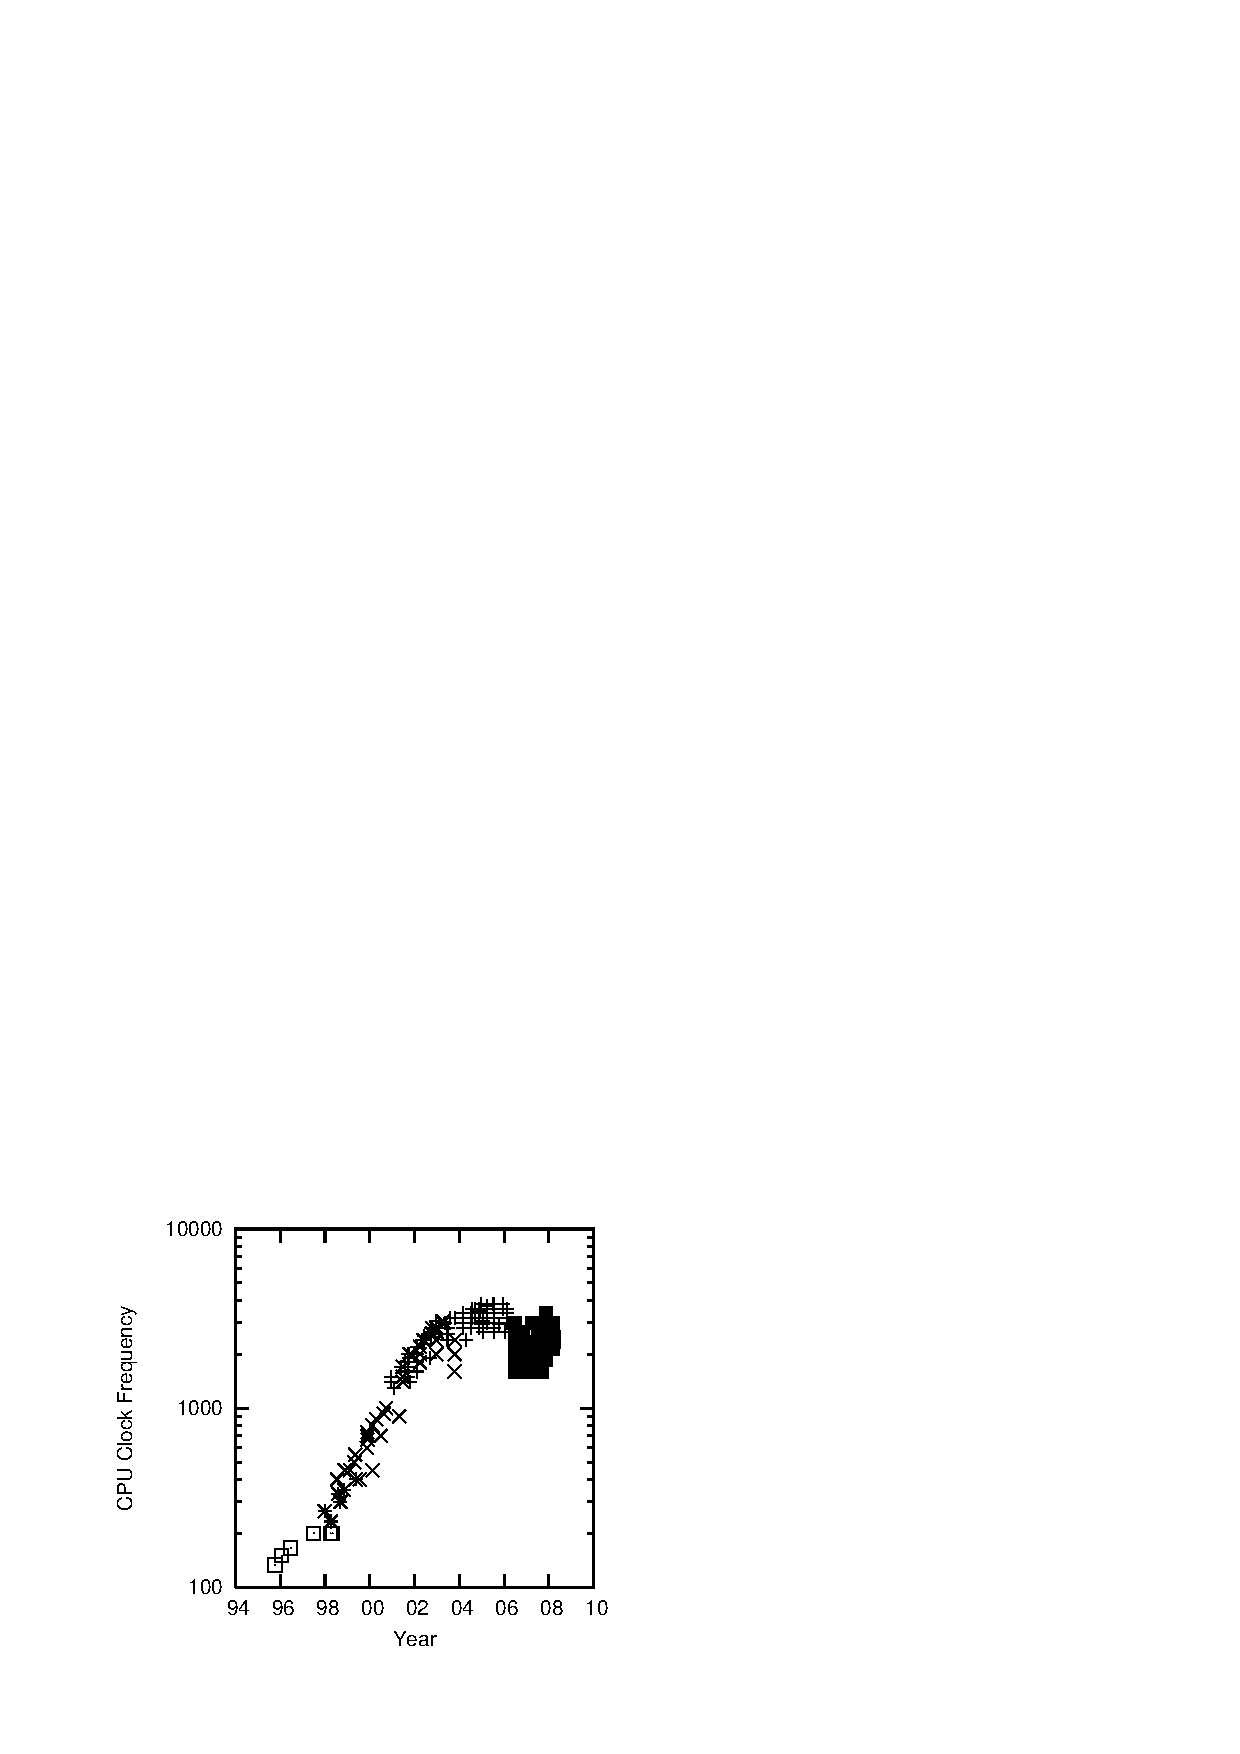
\includegraphics{SMPdesign/clockfreq}}
\end{center}
\caption{MIPS/Clock-Frequency Trend for Intel CPUs}
\label{fig:intro:Clock-Frequency Trend for Intel CPUs}
\end{figure}

That said, the focus of performance has shifted from hardware to
parallel software.
This change in focus is due to the fact that Moore's Law has ceased to
provide its traditional performance
benefits, as can be seen in
Figure~\ref{fig:intro:Clock-Frequency Trend for Intel CPUs}.\footnote{	
	This plot shows clock frequencies for newer CPUs theoretically
	capable of retiring one or more instructions per clock, and MIPS for
	older CPUs requiring multiple clocks to execute even the
	simplest instruction.
	The reason for taking this approach is that the newer CPUs'
	ability to retire multiple instructions per clock is typically
	limited by memory-system performance.}
This means that writing single-threaded code and simply waiting
a years or two for the CPUs to catch up may no longer be an option.
Given the recent trends on the part of all major manufacturers towards
multicore/multithreaded systems, parallelism is the way to go for
those wanting the avail themselves of the full performance of their
systems.

Even so, the first goal is performance rather than scalability,
especially given that the easiest way to attain linear scalability
is to reduce the performance of each CPU~\cite{LinusTorvalds2001a}.
Given a four-CPU system, which would you prefer?
A program that provides 100 transactions per second on a single CPU,
but does not scale at all?
Or a program that provides 10 transactions per second on a single CPU,
but scales perfectly?
The first program seems like a better bet, though the answer might
change if you happened to be one of the lucky few with access to a
32-CPU system.

That said, just because you have multiple CPUs is not necessarily
in and of itself a reason to use them all, especially given the
recent decreases in price of multi-CPU systems.
The key point to understand is that parallel programming is primarily
a performance optimization, and, as such, it is one potential optimization
of many.
If your program is fast enough as currently written, there is no
reason to optimize, either by parallelizing it or by applying any
of a number of potential sequential optimizations.\footnote{
	Of course, if you are a hobbyist whose primary interest is
	writing parallel software, that is more than reason enough to
	parallelize whatever software you are interested in.}
By the same token, if you are looking to apply parallelism as an
optimization to a sequential program, then you will need to compare
parallel algorithms to the best sequential algorithms.
This may require some care, as far too many publications ignore the
sequential case when analyzing the performance of parallel algorithms.

\subsection{Productivity}
\label{sec:intro:Productivity}

\QuickQuiz{}
	Why all this prattling on about non-technical issues???
	And not just \emph{any} non-technical issue, but \emph{productivity}
	of all things???
	Who cares???
\QuickQuizAnswer{
	If you are a pure hobbyist, perhaps you don't need to care.
	But even pure hobbyists will often care about how much they
	can get done, and how quickly.
	After all, the most popular hobbyist tools are usually those
	that are the best suited for the job, and an important part of
	the definition of ``best suited'' involves productivity.
	And if someone is paying you to write parallel code, they will
	very likely care deeply about your productivity.
	And if the person paying you cares about something, you would
	be most wise to pay at least some attention to it!

	Besides, if you \emph{really} didn't care about productivity,
	you would be doing it by hand rather that using a computer!
} \QuickQuizEnd

Productivity has been becoming increasingly important through the decades.
To see this, consider that early computers cost millions of dollars at
a time when engineering salaries were a few thousand dollars a year.
If dedicating a team of ten engineers to such a machine would improve
its performance by 10\%, their salaries would be repaid many times over.

One such machine was the CSIRAC, the oldest still-intact stored-program
computer, put in operation in
1949~\cite{CSIRACMuseumVictoria,CSIRACUniversityMelbourne}.
Given that the machine had but 768 words of RAM, it is safe to say
that the productivity issues that arise in large-scale software projects
were not an issue for this machine.
Because this machine was built before the transistor era, it was constructed
of 2,000 vacuum tubes, ran with a clock frequency of 1kHz,
consumed 30kW of power, and weighed more than three metric tons.

It would be difficult to purchase a machine with this little compute
power roughly sixty years later (2008), with the closest equivalents
being 8-bit embedded microprocessors exemplified by the venerable
Z80~\cite{z80Wikipedia}.
This CPU had 8,500 transistors, and can still be purchased in 2008
for less than \$2 US per unit in 1,000-unit quantities.
In stark contrast to the CSIRAC, software-development costs are
anything but insignificant for the Z80.

\begin{figure}[tb]
\begin{center}
\resizebox{3in}{!}{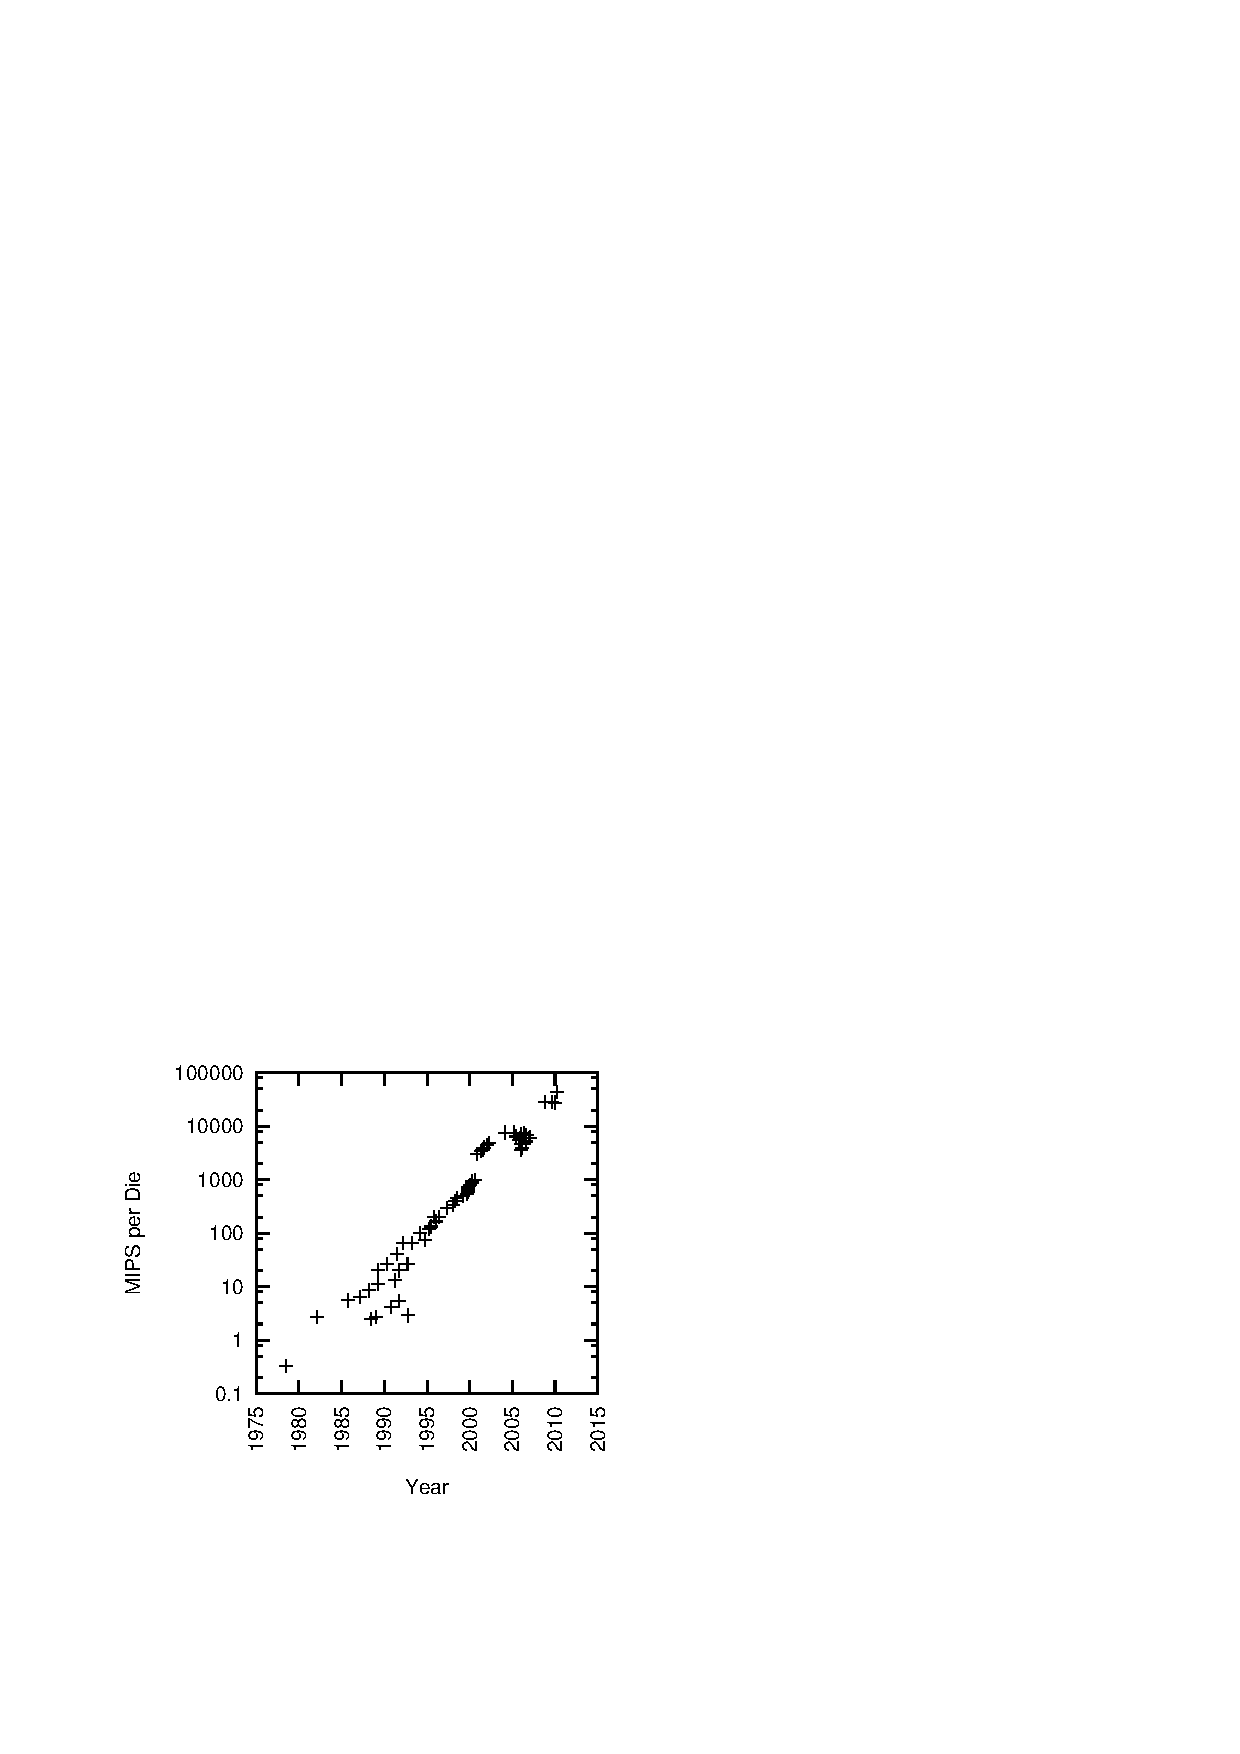
\includegraphics{SMPdesign/mipsperbuck}}
\end{center}
\caption{MIPS per Die for Intel CPUs}
\label{fig:intro:MIPS per Die for Intel CPUs}
\end{figure}

The CSIRAC and the Z80 are two points in a long-term trend, as can be
seen in
Figure~\ref{fig:intro:MIPS per Die for Intel CPUs}.
This figure plots an approximation to computational power per die
over the past three decades, showing a consistent four-order-of-magnitude
increase.
Note that the advent of multicore CPUs has permitted this increase to
continue unabated despite the clock-frequency wall encountered in 2003.

One of the inescapable consequences of the rapid decrease in
the cost of hardware is that software productivity grows increasingly
important.
It is no longer sufficient merely to make efficient use of the hardware,
it is now also necessary to make extremely efficient use of software
developers.
This has long been the case for sequential hardware, but only recently
has parallel hardware become a low-cost commodity.
Therefore, the need for high productivity in creating parallel software
has only recently become hugely important.

\QuickQuiz{}
	Given how cheap parallel hardware has become, how can anyone
	afford to pay people to program it?
\QuickQuizAnswer{
	There are a number of answers to this question:
	\begin{enumerate}
	\item	Given a large computational cluster of parallel machines,
		the aggregate cost of the cluster can easily justify
		substantial developer effort, because the development
		cost can be spread over the large number of machines.
	\item	Popular software that is run by tens of millions of users
		can easily justify substantial developer effort,
		as the cost of this development can be spread over the tens
		of millions of users.
		Note that this includes things like kernels and system
		libraries.
	\item	If the low-cost parallel machine is controlling the operation
		of a valuable piece of equipment, then the cost of this
		piece of equipment might easily justify substantial
		developer effort.
	\item	If the software for the low-cost parallel produces an
		extremely valuable result (e.g., mineral exploration),
		then the valuable result might again justify substantial
		developer cost.
	\item	Safety-critical systems protect lives, which can clearly
		justify very large developer effort.
	\item	Hobbyists and researchers might seek knowledge, experience,
		fun, or glory rather than mere money.
	\end{enumerate}
	So it is not the case that the decreasing cost of hardware renders
	software worthless, but rather that it is no longer possible to
	``hide'' the cost of software development within the cost of
	the hardware, at least not unless there are extremely large
	quantities of hardware.
} \QuickQuizEnd

Perhaps at one time, the sole purpose of parallel software was performance.
Now, however, productivity is increasingly important.

\subsection{Generality}
\label{sec:intro:Generality}

One way to justify the high cost of developing parallel software
is to strive for maximal generality.
All else being equal, the cost of a more-general software artifact
can be spread over more users than can a less-general artifact.

Unfortunately, generality often comes at the cost of performance,
productivity, or both.
To see this, consider the following popular parallel programming
environments:

\begin{description}
\item[C/C++ ``Locking Plus Threads'']: This category, which includes
	POSIX Threads (pthreads)~\cite{OpenGroup1997pthreads},
	Windows Threads, and numerous
	operating-system kernel environments, offers excellent performance
	(at least within the confines of a single SMP system)
	and also offers good generality.
	Pity about the relatively low productivity.
\item[Java]: This programming environment, which is inherently
	multithreaded, is widely believed to be much more productive
	than C or C++, courtesy of the automatic garbage collector
	and the rich set of class libraries, and is reasonably
	general purpose.
	However, its performance, though greatly improved over the past ten
	years, is generally considered to be less than that of C and C++.
\item[MPI]: this message-passing interface~\cite{MPIForum2008} powers
	the largest scientific and technical computing clusters in
	the world, so offers unparalleled performance and scalability.
	It is in theory general purpose, but has generally been used
	for scientific and technical computing.
	It productivity is believed by many to be even less than that
	of C/C++ ``locking plus threads'' environments.
\item[OpenMP]: this set of compiler directives can be used
	to parallelize loops.  It is thus quite specific to this
	task, and this specificity often limits its performance,
	It is, however, much easier to use than MPI or parallel C/C++.
\item[SQL]: structured query language~\cite{DIS9075SQL92} is extremely
	specific, applying only to relational database queries.
	However, its performance is quite good, doing quite well
	in Transaction Processing Performance Council (TPC)
	benchmarks~\cite{TPC}.
	Productivity is excellent, in fact, this parallel programming
	environment permits people who know almost nothing about
	parallel programming to make good use of a large parallel
	machine.
\end{description}

\begin{figure}[tb]
\begin{center}
\resizebox{3in}{!}{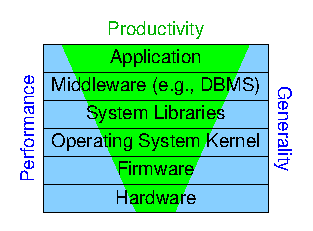
\includegraphics{intro/PPGrelation}}
\end{center}
\caption{Software Layers and Performance, Productivity, and Generality}
\label{fig:intro:Software Layers and Performance, Productivity, and Generality}
\end{figure}

The nirvana of parallel programming environments, one that offers
world-class performance, productivity, and generality, simply does
not yet exist.
Until such a nirvana appears, it will be necessary to make engineering
tradeoffs among performance, productivity, and generality.
One such tradeoff is shown in
Figure~\ref{fig:intro:Software Layers and Performance, Productivity, and Generality},
which shows how productivity becomes increasingly important at the upper layers
of the system stack,
while performance and generality become increasingly important at the
lower layers of the system stack.
The huge development costs incurred near the bottom of the stack
must be spread over equally huge numbers of users on the one hand
(hence the importance of generality), and
performance lost near the bottom of the stack cannot easily be
recovered further up the stack.
Near the top of the stack, there might be very few users for a given
specific application, in which case productivity concerns are paramount.
This explains the tendency towards ``bloatware'' further up the stack:
extra hardware is often cheaper than would be the extra developers.
This book is intended primarily for developers working near the bottom
of the stack, where performance and generality are paramount concerns.

\begin{figure}[tb]
\begin{center}
\resizebox{3in}{!}{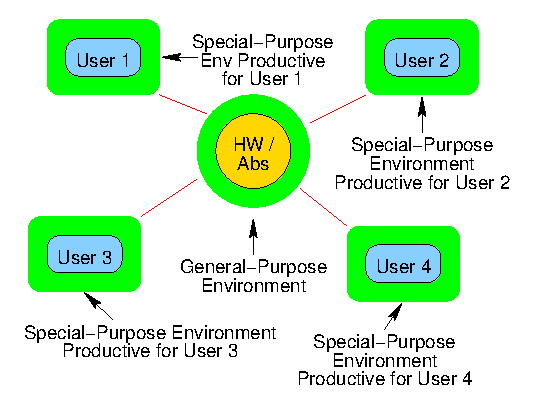
\includegraphics{intro/Generality}}
\end{center}
\caption{Tradeoff Between Productivity and Generality}
\label{fig:intro:Tradeoff Between Productivity and Generality}
\end{figure}

It is important to note that a tradeoff between productivity and
generality has existed for centuries in many fields.
For but one example, a nailgun is far more productive than is a
hammer, but in contrast to the nailgun, a hammer can be used for
many things besides driving nails.
It should therefore be absolutely no surprise to see similar tradeoffs
appear in the field of parallel computing.
This tradeoff is shown schematically in
Figure~\ref{fig:intro:Tradeoff Between Productivity and Generality}.
Here, Users~1, 2, 3, and 4 have specific jobs that they need the computer
to help them with.
The most productive possible language or environment for a given user is one
that simply does that user's job, without requiring any programming,
configuration, or other setup.

\QuickQuiz{}
	This is a ridiculously unachievable ideal!!!
	Why not focus on something that is achievable in practice?
\QuickQuizAnswer{
	This is eminently achievable.
	The cellphone is a computer that can be used to make phone
	calls and to send and receive text messages with little or
	no programming or configuration on the part of the end user.

	This might seem to be a trivial example at first glance,
	but if you consider it carefully you will see that it is
	both simple and profound.
	When we are willing to sacrifice generality, we can achieve
	truly astounding increases in productivity.
	Those who cling to generality will therefore fail to set
	the productivity bar high enough to succeed in production
	environments.
} \QuickQuizEnd

Unfortunately, a system that does the job required by user~1 is
unlikely to do user~2's job.
In other words, the most productive languages and environments are
domain-specific, and thus by definition lacking generality.

Another option is to tailor a given programming language or environment
to the hardware system (for example, low-level languages such as
assembly, C, C++, or Java) or to some abstraction (for example,
Haskell, Prolog, or Snobol), as is shown by the circular region near
the center of
Figure~\ref{fig:intro:Tradeoff Between Productivity and Generality}.
These languages can be considered to be general in the sense that they
are equally ill-suited to the jobs required by users~1, 2, 3, and 4.
In other words, their generality is purchased at the expense of
decreased productivity when compared to domain-specific languages
and environments.

With the three often-conflicting parallel-programming goals of
performance, productivity,
and generality in mind, it is now time to look into avoiding these
conflicts by considering alternatives to
parallel programming.

\section{Alternatives to Parallel Programming}
\label{sec:intro:Alternatives to Parallel Programming}

In order to properly consider alternatives to parallel programming,
you must first have thought through what you expect the parallelism
to do for you.
As seen in Section~\ref{sec:intro:Parallel Programming Goals},
the primary goals of parallel programming are performance, productivity,
and generality.

Although historically most parallel developers might be most concerned
with the first goal,
one advantage of the other goals is that they relieve you of the need
to justify using parallelism.
The remainder of this section is concerned only performance improvement.

It is important to keep in mind that parallelism is but one way to
improve performance.
Other well-known approaches include the following, in roughly increasing
order of difficulty:

\begin{enumerate}
\item	Run multiple instances of a sequential application.
\item	Construct the application to make use of existing parallel software.
\item	Apply performance optimization to the serial application.
\end{enumerate}

\subsection{Multiple Instances of a Sequential Application}
\label{sec:intro:Multiple Instances of a Sequential Application}

Running multiple instances of a sequential application can allow you
to do parallel programming without actually doing parallel programming.
There are a large number of ways to approach this, depending on the
structure of the application.

If your program is analyzing a large number of different scenarios,
or is analyzing a large number of independent data sets, one easy
and effective approach is to create a single sequential program that
carries out a single analysis, then use any of a number of scripting
environments (for example the \url{bash} shell) to run a number of
instances of this sequential program in parallel.
In some cases, this approach can be easily extended to a cluster of
machines.

This approach may seem like cheating, and in fact some denigrate such
programs ``embarrassingly parallel''.
And in fact, this approach does have some potential disadvantages,
including increased memory consumption, waste of CPU cycles recomputing
common intermediate results, and increased copying of data.
However, it is often  extremely effective, garnering extreme performance
gains with little or no added effort.

\subsection{Make Use of Existing Parallel Software}
\label{sec:intro:Make Use of Existing Parallel Software}

There is no longer any shortage of parallel software environments that
can present a single-threaded programming environment,
including relational
databases, web-application servers, and map-reduce environments.
For example, a common design provides a separate program for each
user, each of which generates SQL that is run concurrently against a common
relational database.
The per-user programs are responsible only for the user interface,
with the relational database taking full responsibility for the
difficult issues surrounding parallelism and persistence.

Taking this approach often sacrifices some performance, at least when
compared to carefully hand-coding a fully parallel application.
However, such sacrifice is often justified given the great reduction in
development effort required.

\subsection{Performance Optimization}
\label{sec:intro:Performance Optimization}

Up through the early 2000s, CPU performance was doubling every 18 months.
In such an environment, it is often much more important to create new
functionality than to do careful performance optimization.
Now that Moore's Law is ``only'' increasing transistor density instead
of increasing both transistor density and per-transistor performance,
it might be a good time to rethink the importance of performance
optimization.

After all, performance optimization can reduce power consumption as
well as increasing performance.

From this viewpoint, parallel programming is but another performance
optimization, albeit one that is becoming \emph{much} more attractive
as parallel systems become cheaper and more readily available.
However, it is wise to keep in mind that the speedup available from
parallelism is limited to roughly the number of CPUs, while the
speedup potentially available from straight software optimization
can be multiple orders of magnitude.

Furthermore, different programs might have different performance
bottlenecks.
Parallel programming will only help with some bottlenecks.
For example, suppose that your program spends most of its time
waiting on data from your disk drive.
In this case, making your program use multiple CPUs is not likely
to gain much performance.
In fact, if the program was reading from a large file laid out
sequentially on a rotating disk, parallelizing your program might
well make it a lot slower.
You should instead add more disk drives, optimize the data so that
the file can be smaller (thus faster to read), or, if possible,
avoid the need to read quite so much of the data.

\QuickQuiz{}
	What other bottlenecks might prevent additional CPUs from
	providing additional performance?
\QuickQuizAnswer{
	There are any number of potential bottlenecks:
	\begin{enumerate}
	\item	Main memory.  If a single thread consumes all available
		memory, additional threads will simply page themselves
		silly.
	\item	Cache.  If a single thread's cache footprint completely
		fills any shared CPU cache(s), then adding more threads
		will simply thrash the affected caches.
	\item	Memory bandwidth.  If a single thread consumes all available
		memory bandwidth, additional threads will simply
		result in additional queuing on the system interconnect.
	\item	I/O bandwidth.  If a single thread is I/O bound,
		adding more threads will simply result in them all
		waiting in line for the affected I/O resource.
	\end{enumerate}

	Specific hardware systems may have any number of additional
	bottlenecks.
} \QuickQuizEnd

Parallelism can be a powerful optimization technique, but
it is not the only such technique, nor is it appropriate for all
situations.
Of course, the easier it is to parallelize your program, the
more attractive parallelization becomes as an optimization.
Parallelization has a reputation of being quite difficult,
which leads to the question ``exactly what makes parallel
programming so difficult?''

\section{What Makes Parallel Programming Hard?}
\label{sec:intro:What Makes Parallel Programming Hard?}

\OriginallyPublished{Section}{sec:intro:What Makes Parallel Programming Hard?}{What Makes Parallel Programming Hard?}{a Portland State University Technical Report}{PaulEMcKenney2009ProgrammingHard}

It is important to note that the difficulty of parallel programming
is as much a human-factors issue as it is a set of technical properties of the
parallel programming problem.
This is the case because we need human beings to be able to tell parallel
systems what to do, and this two-way communication between human and
computer is as much a function of the human as it is of the computer.
Therefore, appeals to abstractions or to mathematical analyses will
necessarily be of severely limited utility.

In the Industrial Revolution, the interface between human and machine
was evaluated by human-factor studies, then called time-and-motion
studies.
Although there have been a few human-factor studies examining parallel
programming~\cite{RyanEccles2005HPCSNovice,RyanEccles2006HPCSNoviceNeeds,
LorinHochstein2005SC,DuaneSzafron1994PEMPDS}, these studies have
been extremely narrowly focused, and hence unable to demonstrate any
general results.
Furthermore, given that the normal range of programmer productivity
spans more than an order of magnitude, it is unrealistic to expect
an affordable study to be capable of detecting (say) a 10\% difference
in productivity.
Although the multiple-order-of-magnitude differences that such studies
\emph{can} reliably detect are extremely valuable, the most impressive
improvements tend to be based on a long series of 10\% improvements.

We must therefore take a different approach.

\begin{figure}[tb]
\begin{center}
\resizebox{3in}{!}{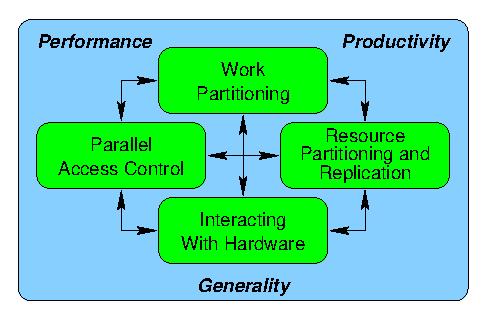
\includegraphics{intro/FourTaskCategories}}
\end{center}
\caption{Categories of Tasks Required of Parallel Programmers}
\label{fig:intro:Categories of Tasks Required of Parallel Programmers}
\end{figure}

One such approach is to carefully consider what tasks that parallel
programmers must undertake that are not required of sequential programmers.
We can then evaluate how well a given programming language or environment
assists the developer with these tasks.
These tasks fall into the four categories shown in
Figure~\ref{fig:intro:Categories of Tasks Required of Parallel Programmers},
each of which is covered in the following sections.

\subsection{Work Partitioning}
\label{sec:intro:Work Partitioning}

Work partitioning is absolutely required for parallel execution:
if there is but one ``glob'' of work, then it can be executed by at
most one CPU at a time, which is by definition sequential execution.
However, partitioning the code requires great care.
For example, uneven partitioning can result in sequential execution
once the small partitions have completed~\cite{GeneAmdahl1967AmdahlsLaw}.
In less extreme cases, load balancing can be used to fully utilize
available hardware, thus attaining more-optimal performance.

In addition, partitioning of work can complicate handling of global
errors and events: a parallel
program may need to carry out non-trivial synchronization in order
to safely process such global events.

Each partition requires some sort of communication: after all, if
a given thread did not communicate at all, it would have no effect and
would thus not need to be executed.
However, because communication incurs overhead, careless partitioning choices
can result in severe performance degradation.

Furthermore, the number of concurrent threads must often be controlled,
as each such thread occupies common resources, for example,
space in CPU caches.
If too many threads are permitted to execute concurrently, the
CPU caches will overflow, resulting in high cache miss rate, which in
turn degrades performance.
On the other hand, large numbers of threads are often required to
overlap computation and I/O.

\QuickQuiz{}
	What besides CPU cache capacity might require limiting the
	number of concurrent threads?
\QuickQuizAnswer{
	There are any number of potential limits on the number of
	threads:
	\begin{enumerate}
	\item	Main memory.  Each thread consumes some memory
		(for its stack if nothing else), so that excessive
		numbers of threads can exhaust memory, resulting
		in excessive paging or memory-allocation failures.
	\item	I/O bandwidth.  If each thread initiates a given
		amount of mass-storage I/O or networking traffic,
		excessive numbers of threads can result in excessive
		I/O queuing delays, again degrading performance.
		Some networking protocols may be subject to timeouts
		or other failures if there are so many threads that
		networking events cannot be responded to in a timely
		fashion.
	\item	Synchronization overhead.
		For many synchronization protocols, excessive numbers
		of threads can result in excessive spinning, blocking,
		or rollbacks, thus degrading performance.
	\end{enumerate}

	Specific applications and platforms may have any number of additional
	limiting factors.
} \QuickQuizEnd

Finally, permitting threads to execute concurrently greatly increases
the program's state space, which can make the program difficult to
understand, degrading productivity.
All else being equal, smaller state spaces having more regular structure
are more easily understood, but this is a human-factors statement as opposed
to a technical or mathematical statement.
Good parallel designs might have extremely large state spaces, but
nevertheless be easy to understand due to their regular structure,
while poor designs can be impenetrable despite having a comparatively
small state space.
The best designs exploit embarrassing parallelism, or transform the
problem to one having an embarrassingly parallel solution.
In either case, ``embarrassingly parallel'' is in fact
an embarrassment of riches.
The current state of the art enumerates good designs; more work is
required to make more general judgements on
state-space size and structure.

\subsection{Parallel Access Control}
\label{sec:Parallel Access Control}

Given a sequential program with only a single thread, that single
thread has full access to all of the program's resources.
These resources are most often in-memory data structures, but can be CPUs,
memory (including caches), I/O devices, computational accelerators, files,
and much else besides.

The first parallel-access-control issue is whether the form of the access to
a given resource depends on that resource's location.
For example, in many message-passing environments, local-variable
access is via expressions and assignments,
while remote-variable access uses an entirely different
syntax, usually involving messaging.
The POSIX threads environment~\cite{OpenGroup1997pthreads},
Structured Query Language (SQL)~\cite{DIS9075SQL92}, and
partitioned global address-space (PGAS) environments
such as Universal Parallel C (UPC)~\cite{ElGhazawi2003UPC}
offer implicit access,
while Message Passing Interface (MPI)~\cite{MPIForum2008} offers
explicit access because access to remote data requires explicit
messaging.

The other parallel access-control issue is how threads coordinate
access to the resources.
This coordination is carried out by
the very large number of synchronization mechanisms
provided by various parallel languages and environments,
including message passing, locking, transactions,
reference counting, explicit timing, shared atomic variables, and data
ownership.
Many traditional parallel-programming concerns such as deadlock,
livelock, and transaction rollback stem from this coordination.
This framework can be elaborated to include comparisons
of these synchronization mechanisms, for example locking vs. transactional
memory~\cite{McKenney2007PLOSTM}, but such elaboration is beyond the
scope of this section.

\subsection{Resource Partitioning and Replication}
\label{sec:Resource Partitioning and Replication}

The most effective parallel algorithms and systems exploit resource
parallelism, so much so that it is
usually wise to begin parallelization by partitioning your write-intensive
resources and replicating frequently accessed read-mostly resources.
The resource in question is most frequently data, which might be
partitioned over computer systems, mass-storage devices, NUMA nodes,
CPU cores (or dies or hardware threads), pages, cache lines, instances
of synchronization primitives, or critical sections of code.
For example, partitioning over locking primitives is termed
``data locking''~\cite{Beck85}.

Resource partitioning is frequently application dependent, for
example, numerical applications frequently partition matrices
by row, column, or sub-matrix, while commercial applications frequently
partition write-intensive data structures and replicate
read-mostly data structures.
For example, a commercial application might assign the data for a
given customer to a given few computer systems out of a large cluster.
An application might statically partition data, or dynamically
change the partitioning over time.

Resource partitioning is extremely effective, but
it can be quite challenging for complex multilinked data
structures.

\subsection{Interacting With Hardware}
\label{sec:Interacting With Hardware}

Hardware interaction is normally the domain of the operating system,
the compiler, libraries, or other software-environment infrastructure.
However, developers working with novel hardware features and components
will often need to work directly with such hardware.
In addition, direct access to the hardware can be required when squeezing
the last drop of performance out of a given system.
In this case, the developer may need to tailor or configure the application
to the cache geometry, system topology, or interconnect protocol of the
target hardware.

In some cases, hardware may be considered to be a resource which
may be subject to partitioning or access control, as described in
the previous sections.

\subsection{Composite Capabilities}
\label{sec:Composite Capabilities}

Although these four capabilities are fundamental,
good engineering practice uses composites of
these capabilities.
For example, the data-parallel approach first
partitions the data so as to minimize the need for
inter-partition communication, partitions the code accordingly,
and finally maps data partitions and threads so as to maximize
throughput while minimizing inter-thread communication.
The developer can then
consider each partition separately, greatly reducing the size
of the relevant state space, in turn increasing productivity.
Of course, some problems are non-partitionable but on the other hand,
clever transformations into forms permitting partitioning can greatly
enhance
both performance and scalability~\cite{PanagiotisMetaxas1999PDCS}.

\subsection{How Do Languages and Environments Assist With These Tasks?}
\label{sec:intro:How Do Languages and Environments Assist With These Tasks?}

Although many environments require that the developer deal manually
with these tasks, there are long-standing environments that bring
significant automation to bear.
The poster child for these environments is SQL, many implementations
of which automatically parallelize single large queries and also
automate concurrent execution of independent queries and updates.

These four categories of tasks must be carried out in all parallel
programs, but that of course does not necessarily mean that the developer
must manually carry out these tasks.
We can expect to see ever-increasing automation of these four tasks
ask parallel systems continue to become cheaper and more readily available.

\QuickQuiz{}
	Are there any other obstacles to parallel programming?
\QuickQuizAnswer{
	There are a great many other potential obstacles to parallel
	programming.
	Here are a few of them:
	\begin{enumerate}
	\item	The only known algorithms for a given project might
		be inherently sequential in nature.
		In this case, either avoid parallel programming
		(there being no law saying that your project \emph{has}
		to run in parallel) or invent a new parallel algorithm.
	\item	The project allows binary-only plugins that share the same
		address space, such that no one developer has access to
		all of the source code for the project.
		Because many parallel bugs, including deadlocks, are
		global in nature, such binary-only plugins pose a severe
		challenge to current software development methodologies.
		This might well change, but for the time being, all
		developers of parallel code sharing a given address space
		need to be able to see \emph{all} of the code running in
		that address space.
	\item	The project contains heavily used APIs that were designed
		without regard to parallelism.
		Some of the more ornate features of the System V
		message-queue API form a case in point.
		Of course, if your project has been around for a few
		decades, and if its developers did not have access to
		parallel hardware, your project undoubtedly has at least
		its share of such APIs.
	\item	The project was implemented without regard to parallelism.
		Given that there are a great many techniques that work
		extremely well in a sequential environment, but that
		fail miserably in parallel environments, if your project
		ran only on sequential hardware for most of its lifetime,
		then your project undoubtably has at least its share of
		parallel-unfriendly code.
	\item	The project was implemented without regard to good
		software-development practice.
		The cruel truth is that shared-memory parallel
		environments are often much less forgiving of sloppy
		development practices than are sequential environments.
		You may be well-served to clean up the existing design
		and code prior to attempting parallelization.
	\item	The people who originally did the development on your
		project have since moved on, and the people remaining,
		while well able to maintain it or add small features,
		are unable to make ``big animal'' changes.
		In this case, unless you can work out a very simple
		way to parallelize your project, you will probably
		be best off leaving it sequential.
		That said, there are a number of simple approaches that
		you might use
		to parallelize your project, including running multiple
		instances of it, using a parallel implementation of
		some heavily used library function, or making use of
		some other parallel project, such as a database.
	\end{enumerate}

	One can argue that many of these obstacles are non-technical
	in nature, but that does not make them any less real.
	In short, parallelization can be a large and complex effort.
	As with any large and complex effort, it makes sense to
	do your homework beforehand.
} \QuickQuizEnd

\section{Guide to This Book}
\label{sec:intro:Guide to This Book}

This book is not a collection of optimal algorithms with tiny areas of
applicability; instead, it is a handbook of widely applicable and heavily
used techniques.
We of course could not resist the urge to include some of our favorites
that have not (yet!) passed the test of time (what author could?), but
we have nonetheless gritted our teeth and banished our darlings to
appendices.
Perhaps in time, some of them will see enough use that we can promote
them into the main body of the text.

% \emph{@@@ More here.  Sections.  Layered Approach.  Appendices.
% Glossary.  Bibliography.}

\subsection{Quick Quizzes}

``Quick quizzes'' appear throughout this book.
Some of these quizzes are based on material in which that quick quiz
appears, but others require you to think beyond that section, and,
in some cases, beyond the entire book.
As with most endeavors, what you get out of this book is largely
determined by what you are willing to put into it.
Therefore, readers who invest some time into these quizzes will
find their effort repaid handsomely with increased understanding
of parallel programming.

Answers to the quizzes may be found
in
Appendix~\ref{chp:Answers to Quick Quizzes} starting on
page~\pageref{chp:Answers to Quick Quizzes}.

\QuickQuiz{}
	Where are the answers to the Quick Quizzes found?
\QuickQuizAnswer{
	In Appendix~\ref{chp:Answers to Quick Quizzes} starting on
	page~\pageref{chp:Answers to Quick Quizzes}.

	Hey, I thought I owed you an easy one!!!
} \QuickQuizEnd

\QuickQuiz{}
	Some of the Quick Quiz questions seem to be from the viewpoint
	of the reader rather than the author.
	Is that really the intent?
\QuickQuizAnswer{
	Indeed it is!
	Many are modeled after Paul---just ask anyone who has had the
	misfortune of being assigned to teach him.
	Others are quite similar to actual questions that have been asked
	during conference presentations and lectures covering the
	material in this book.
	Still others are from the viewpoint of the author.
} \QuickQuizEnd

\QuickQuiz{}
	These Quick Quizzes just are not my cup of tea.
	What do you recommend?
\QuickQuizAnswer{
	There are a number of alternatives available to you:
	\begin{enumerate}
	\item	Just ignore the Quick Quizzes and read the rest of
		the book.
		You might miss out on the interesting material in
		some of the Quick Quizzes, but the rest of the book
		has lots of good material as well.
	\item	If you prefer a more academic and rigorous treatment of
		parallel programming,
		you might like Herlihy's and Shavit's
		textbook~\cite{HerlihyShavit2008Textbook}.
		This book starts with an interesting combination
		of low-level primitives at high levels of abstraction
		from the hardware, and works its way through locking
		and simple data structures including lists, queues,
		hash tables, and counters, culminating with transactional
		memory.
	\item	If you would like an academic treatment of parallel
		programming that keeps to a more pragmatic viewpoint,
		you might be interested in the concurrency chapter from Scott's
		textbook~\cite{MichaelScott2006Textbook}
		on programming languages.
	\item	If you are interested in an object-oriented patternist
		treatment of parallel programming focussing on C++,
		you might try Volumes~2 and 4 of Schmidt's POSA
		series~\cite{SchmidtStalRohnertBuschmann2000v2Textbook,
		BuschmannHenneySchmidt2007v4Textbook}.
		Volume 4 in particular has some interesting chapters
		applying this work to a warehouse application.
		The realism of this example is attested to by
		the section entitled ``Partitioning the Big Ball of Mud'',
		wherein the problems inherent in parallelism often
		take a back seat to the problems inherent in getting
		one's head around a real-world application.
	\item	If your primary focus is scientific and technical computing,
		and you prefer a patternist approach,
		you might try Mattson et al.'s
		textbook~\cite{Mattson2005Textbook}.
		It covers Java, C/C++, OpenMP, and MPI.
		Its patterns are admirably focused first on design,
		then on implementation.
	\item	If you are interested in POSIX Threads, you might take
		a look at David R. Butenhof's book~\cite{Butenhof1997pthreads}.
	\item	If you are interested in C++, but in a Windows environment,
		you might try Herb Sutter's ``Effective Concurrency''
		series in
		Dr. Dobbs Journal~\cite{HerbSutter2008EffectiveConcurrency}.
		This series does a reasonable job of presenting a
		commonsense approach to parallelism.
	\item	If you want to try out Intel Threading Building Blocks,
		then perhaps James Reinders's book~\cite{Reinders2007Textbook}
		is what you are looking for.
	\item	Finally, those preferring to work in Java might be
		well-served by Doug Lea's
		textbooks~\cite{DougLea1997Textbook,Goetz2007Textbook}.
	\end{enumerate}
	In contrast, this book meshes real-world machines with real-world
	algorithms.
	If your sole goal is to find an optimal parallel queue, you might
	be better served by one of the above books.
	However, if you are interested in principles of parallel design
	that allow multiple such queues to operate in parallel, read on!
} \QuickQuizEnd

\subsection{Sample Source Code}

This book discusses its fair share of source code, and in many cases
this source code may be found in the \url{CodeSamples} directory
of this book's git tree.
For example, on UNIX systems, you should be able to type:
\begin{verbatim}
	find CodeSamples -name rcu_rcpls.c -print
\end{verbatim}
to locate the file \url{rcu_rcpls.c}, which is called out in
Section~\ref{defer:``Toy'' RCU Implementations}.
Other types of systems have well-known ways of locating files by
filename.

The source to this book may be found in the \url{git} archive at
\url{git://git.kernel.org/pub/scm/linux/kernel/git/paulmck/perfbook.git},
and \url{git} itself is available as part of most mainstream Linux
distributions.
PDFs of this book are sporadically posted at
\url{http://kernel.org/pub/linux/kernel/people/paulmck/perfbook/perfbook.html}.

% cpu/cpu.tex

\QuickQuizChapter{chp:Hardware and its Habits}{Hardware and its Habits}

Most people have an intuitive understanding that passing messages between
systems is considerably more expensive than performing simple calculations
within the confines of a single system.
However, it is not always so clear that communicating among threads within
the confines of a single shared-memory system can also be quite expensive.
This chapter therefore looks the cost of synchronization and communication
within a shared-memory system.
This chapter merely scratches the surface of shared-memory parallel
hardware design; readers desiring more detail would do well to start
with a recent edition of
Hennessy and Patterson's classic text~\cite{Hennessy95a}.

\QuickQuiz{}
	Why should parallel programmers bother learning low-level
	properties of the hardware?
	Wouldn't it be easier, better, and more general to remain at
	a higher level of abstraction?
\QuickQuizAnswer{
	It might well be easier to ignore the detailed properties of
	the hardware, but in most cases it would be quite foolish
	to do so.
	If you accept that the only purpose of parallelism is to
	increase performance, and if you further accept that
	performance depends on detailed properties of the hardware,
	then it logically follows that parallel programmers are going
	to need to know at least a few hardware properties.

	This is the case in most engineering disciplines.
	Would \emph{you} want to use a bridge designed by an
	engineer who did not understand the properties of
	the concrete and steel making up that bridge?
	If not, why would you expect a parallel programmer to be
	able to develop competent parallel software without at least
	\emph{some} understanding of the underlying hardware?
} \QuickQuizEnd

% cpu/overview.tex

\section{Overview}
\label{sec:cpu:Overview}

Careless reading of computer-system specification sheets might lead one
to believe that CPU performance is a footrace on a clear track, as
illustrated in Figure~\ref{fig:cpu:CPU Performance at its Best},
where the race always goes to the swiftest.

\begin{figure}[htb]
\begin{center}
\resizebox{3in}{!}{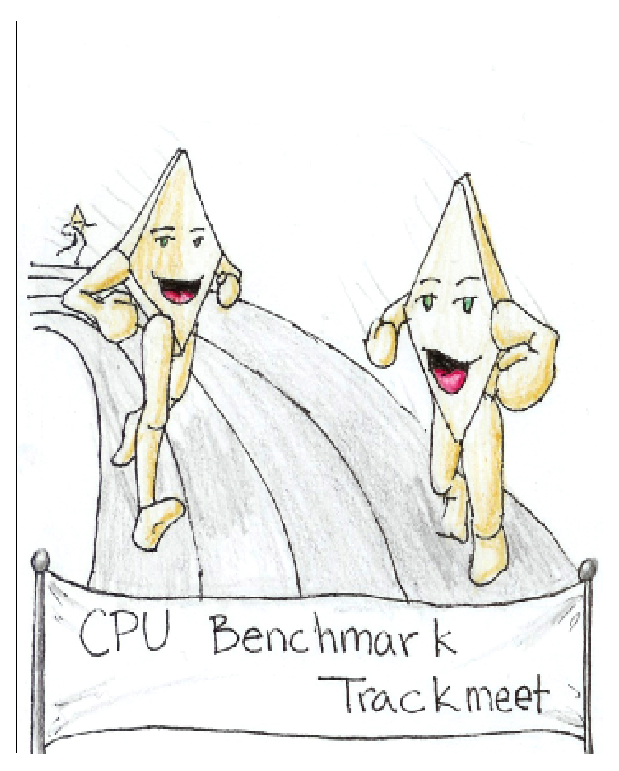
\includegraphics{cartoons/trackmeet}}
\end{center}
\caption{CPU Performance at its Best}
\ContributedBy{Figure}{fig:cpu:CPU Performance at its Best}{Melissa McKenney}
\end{figure}

Although there are a few CPU-bound benchmarks that approach the ideal
shown in Figure~\ref{fig:cpu:CPU Performance at its Best},
the typical program more closely resembles an obstacle course than
a race track.
This is because the internal architecture of CPUs has changed dramatically
over the past few decades, courtesy of Moore's Law.
These changes are described in the following sections.

\subsection{Pipelined CPUs}
\label{sec:cpu:Pipelined CPUs}

\begin{figure}[htb]
\begin{center}
\resizebox{3in}{!}{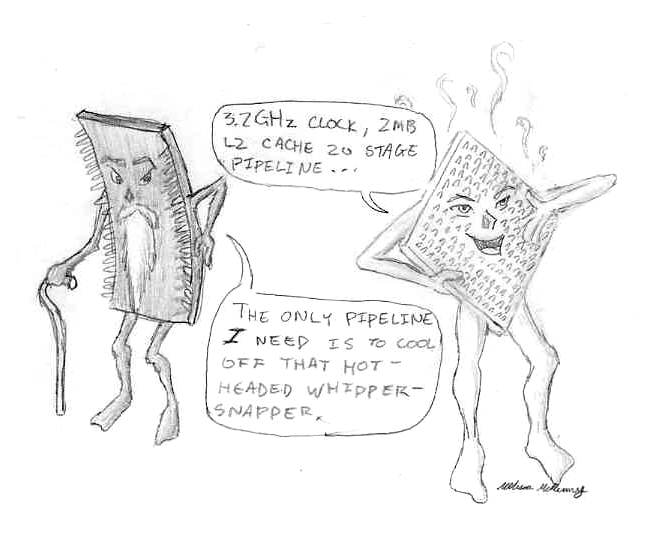
\includegraphics{cartoons/whippersnapper}}
\end{center}
\caption{CPUs Old and New}
\ContributedBy{Figure}{fig:cpu:CPUs Old and New}{Melissa McKenney}
\end{figure}

In the early 1980s, the typical microprocessor fetched an instruction,
decoded it, and executed it, typically taking \emph{at least} three
clock cycles to complete one instruction before proceeding to the next.
In contrast, the CPU of the late 1990s and early 2000s will be executing
many instructions simultaneously, using a deep ``pipeline'' to control
the flow of instructions internally to the CPU, this difference being
illustrated by Figure~\ref{fig:cpu:CPUs Old and New}.

Achieving full performance with a CPU having a long pipeline requires
highly predictable control flow through the program.
Suitable control flow can be provided by a program that executes primarily
in tight loops, for example, programs doing arithmetic on large matrices
or vectors.
The CPU can then correctly predict that the branch at the end of the loop
will be taken in almost all cases.
In such programs, the pipeline can be kept full and the CPU can execute
at full speed.

\begin{figure}[htb]
\begin{center}
\resizebox{3in}{!}{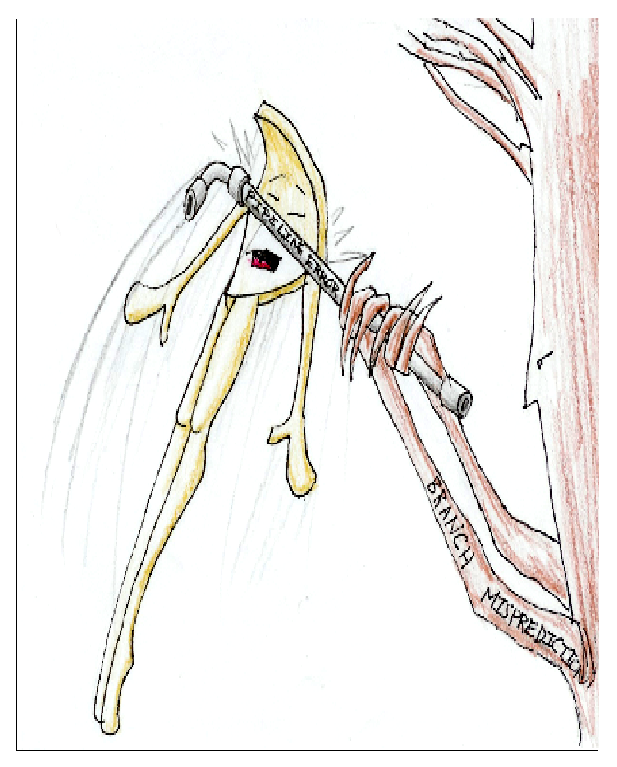
\includegraphics{cartoons/pipeline}}
\end{center}
\caption{CPU Meets a Pipeline Flush}
\ContributedBy{Figure}{fig:cpu:CPU Meets a Pipeline Flush}{Melissa McKenney}
\end{figure}

If, on the other hand, the program has many loops with small loop counts,
or if the program is object oriented with many virtual objects that
can reference many different real objects, all with different implementations
for frequently invoked member functions, then it is difficult or even
impossible for the CPU to predict where a given branch might lead.
The CPU must then either stall waiting for execution to proceed far enough
to know for certain where the branch will lead, or guess --- and, in the
face of programs with unpredictable control flow, frequently guess wrong.
In either case, the pipeline will empty and have to be refilled, leading
to stalls that can drastically reduce performance,
as fancifully depicted in Figure~\ref{fig:cpu:CPU Meets a Pipeline Flush}.

Unfortunately, pipeline flushes are not the only hazards in the obstacle
course that modern CPUs must run.
The next section covers the hazards of referencing memory.

\subsection{Memory References}
\label{sec:cpu:Memory References}

In the 1980s, it often took less time for a microprocessor to load a value
from memory than it did to execute an instruction.
In 2006, a microprocessor might be capable of executing hundreds or even
thousands of instructions in the time required to access memory.
This disparity is due to the fact that Moore's Law has increased CPU
performance at a much greater rate than it has increased memory
performance, in part due to the rate at which memory sizes have
grown.
For example, a typical 1970s minicomputer might have 4KB (yes, kilobytes,
not megabytes, let alone gigabytes) of main memory, with single-cycle access.
In 2008, CPU designers still can construct a 4KB memory with single-cycle
access, even on systems with multi-GHz clock frequencies.
And in fact they frequently do construct such memories, but they now
call them ``level-0 caches''.

Although the large caches found on modern microprocessors can do quite
a bit to help combat memory-access latencies,
these caches require highly predictable data-access patterns to
successfully hide memory latencies.
Unfortunately, common operations, such as traversing a linked list,
have extremely unpredictable memory-access patterns --- after all,
if the pattern was predictable, us software types would not bother
with the pointers, right?

\begin{figure}[htb]
\begin{center}
\resizebox{3in}{!}{
\includegraphics{cartoons/ref}}
\end{center}
\caption{CPU Meets a Memory Reference}
\ContributedBy{Figure}{fig:cpu:CPU Meets a Memory Reference}{Melissa McKenney}
\end{figure}

Therefore, as shown in
Figure~\ref{fig:cpu:CPU Meets a Memory Reference},
memory references are often severe obstacles for modern CPUs.

Thus far, we have only been considering obstacles that can arise during
a given CPU's execution of single-threaded code.
Multi-threading presents additional obstacles to the CPU, as
described in the following sections.

\subsection{Atomic Operations}
\label{sec:cpu:Atomic Operations}

One such obstacle is atomic operations.
The whole idea of an atomic operation in some sense conflicts with
the piece-at-a-time assembly-line operation of a CPU pipeline.
To hardware designers' credit, modern CPUs use a number of extremely clever
tricks to make such operations \emph{look} atomic even though they
are in fact being executed piece-at-a-time, but even so, there are
cases where the pipeline must be delayed or even flushed in order to
permit a given atomic operation to complete correctly.

\begin{figure}[htb]
\begin{center}
\resizebox{3in}{!}{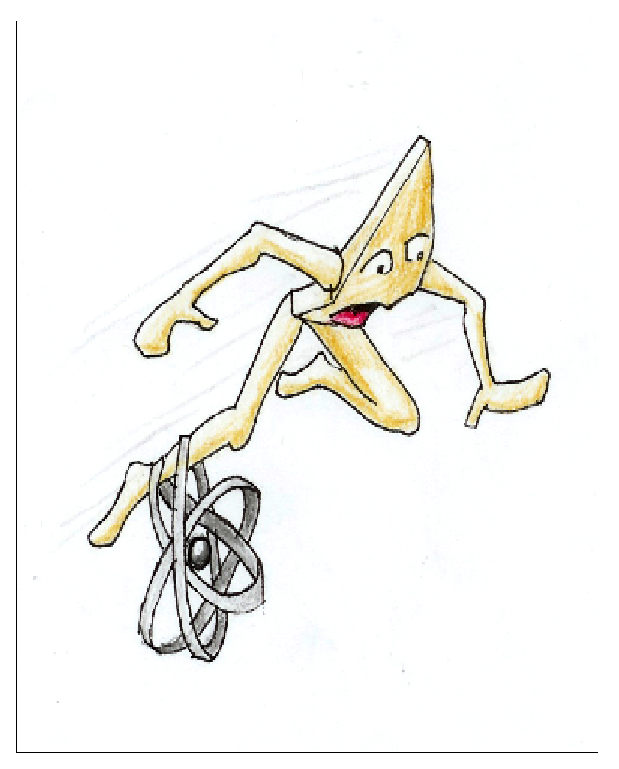
\includegraphics{cartoons/atomic}}
\end{center}
\caption{CPU Meets an Atomic Operation}
\ContributedBy{Figure}{fig:cpu:CPU Meets an Atomic Operation}{Melissa McKenney}
\end{figure}

The resulting effect on performance is depicted in
Figure~\ref{fig:cpu:CPU Meets an Atomic Operation}.

Unfortunately, atomic operations usually apply only to single elements
of data.
Because many parallel algorithms require that ordering constraints
be maintained between updates of multiple data elements, most CPUs
provide memory barriers.
These memory barriers also serve as performance-sapping obstacles,
as described in the next section.

\QuickQuiz{}
	What types of machines would allow atomic operations on
	multiple data elements?
\QuickQuizAnswer{
	One answer to this question is that it is often possible to
	pack multiple elements of data into a single machine word,
	which can then be manipulated atomically.

	A more trendy answer would be machines supporting transactional
	memory~\cite{DBLomet1977SIGSOFT}.
	However, such machines are still (as of 2008) research
	curiosities.
	The jury is still out on the applicability of transactional
	memory~\cite{McKenney2007PLOSTM,DonaldEPorter2007TRANSACT,
	ChistopherJRossbach2007a}.
} \QuickQuizEnd

\subsection{Memory Barriers}
\label{sec:cpu:Memory Barriers}

Memory barriers will be considered in more detail in
Section~\ref{sec:advsync:Memory Barriers} and
Appendix~\ref{chp:app:whymb:Why Memory Barriers?}.
In the meantime, consider the following simple lock-based critical
section:

\vspace{5pt}
\begin{minipage}[t]{\columnwidth}
\small
\begin{verbatim}
  1 spin_lock(&mylock);
  2 a = a + 1;
  3 spin_unlock(&mylock);
\end{verbatim}
\end{minipage}
\vspace{5pt}

\begin{figure}[tb]
\begin{center}
\resizebox{3in}{!}{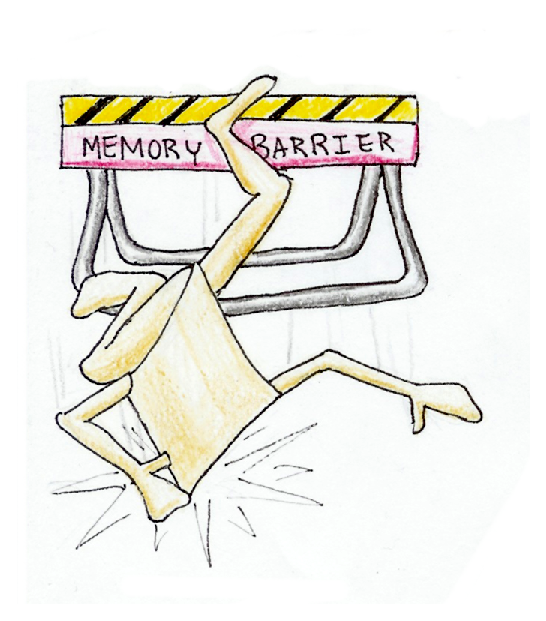
\includegraphics{cartoons/barrier}}
\end{center}
\caption{CPU Meets a Memory Barrier}
\ContributedBy{Figure}{fig:cpu:CPU Meets a Memory Barrier}{Melissa McKenney}
\end{figure}

If the CPU were not constrained to execute these statements in the
order shown, the effect would be that the variable ``a'' would be
incremented without the protection of ``mylock'', which would certainly
defeat the purpose of acquiring it.
To prevent such destructive reordering, locking primitives contain
either explicit or implicit memory barriers.
Because the whole purpose of these memory barriers is to prevent reorderings
that the CPU would otherwise undertake in order to increase performance,
memory barriers almost always reduce performance, as depicted in
Figure~\ref{fig:cpu:CPU Meets a Memory Barrier}.

\subsection{Cache Misses}
\label{sec:cpu:Cache Misses}

\begin{figure}[htb]
\begin{center}
\resizebox{3in}{!}{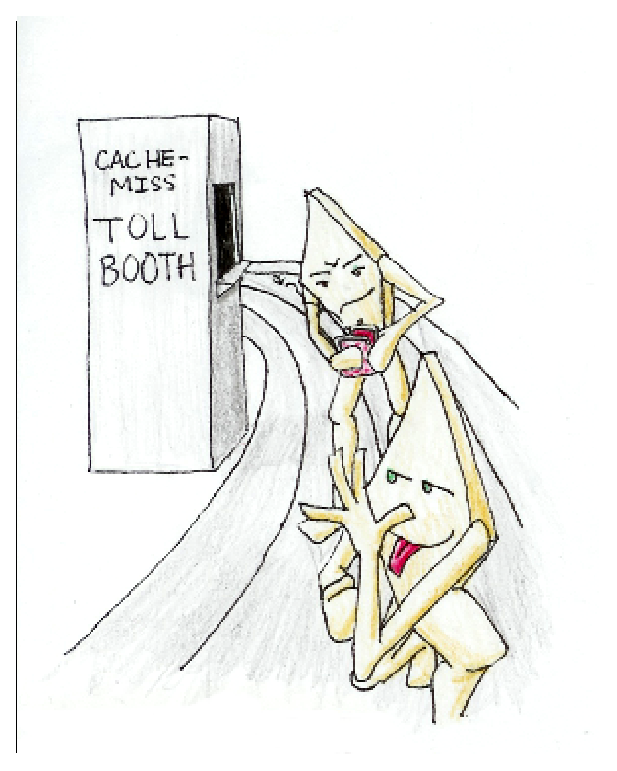
\includegraphics{cartoons/tollbooth}}
\end{center}
\caption{CPU Meets a Cache Miss}
\ContributedBy{Figure}{fig:cpu:CPU Meets a Cache Miss}{Melissa McKenney}
\end{figure}

An additional multi-threading obstacle to CPU performance is
the ``cache miss''.
As noted earlier, modern CPUs sport large caches in order to reduce the
performance penalty that would otherwise be incurred due to slow memory
latencies.
However, these caches are actually counter-productive for variables that
are frequently shared among CPUs.
This is because when a given CPU wishes to modify the variable, it is
most likely the case that some other CPU has modified it recently.
In this case, the variable will be in that other CPU's cache, but not
in this CPU's cache, which will therefore incur an expensive cache miss
(see Section~\ref{sec:app:whymb:Cache Structure} for more detail).
Such cache misses form a major obstacle to CPU performance, as shown
in Figure~\ref{fig:cpu:CPU Meets a Cache Miss}.

\subsection{I/O Operations}
\label{sec:cpu:I/O Operations}

\begin{figure}[htb]
\begin{center}
\resizebox{3in}{!}{\includegraphics{cartoons/PhoneBooth}}
\end{center}
\caption{CPU Waits for I/O Completion}
\ContributedBy{Figure}{fig:cpu:CPU Waits for I/O Completion}{Melissa McKenney}
\end{figure}

A cache miss can be thought of as a CPU-to-CPU I/O operation, and as
such is one of the cheapest I/O operations available.
I/O operations involving networking, mass storage, or (worse yet) human
beings pose much greater obstacles than the internal obstacles called
out in the prior sections,
as illustrated by
Figure~\ref{fig:cpu:CPU Waits for I/O Completion}.

This is one of the differences between shared-memory and distributed-system
parallelism: shared-memory parallel programs must normally deal with no
obstacle worse than a cache miss, while a distributed parallel program
will typically incur the larger network communication latencies.
In both cases, the relevant latencies can be thought of as a cost of
communication---a cost that would be absent in a sequential program.
Therefore, the ratio between the overhead of the communication to
that of the actual work being performed is a key design parameter.
A major goal of parallel design is to reduce this ratio as needed to
achieve the relevant performance and scalability goals.

Of course, it is one thing to say that a given operation is an obstacle,
and quite another to show that the operation is a \emph{significant}
obstacle.
This distinction is discussed in the following sections.

% cpu/overheads.tex

\section{Overheads}
\label{sec:cpu:Overheads}

This section presents actual overheads of the obstacles to performance
listed out in the previous section.
However, it is first necessary to get a rough view of hardware system
architecture, which is the subject of the next section.

\subsection{Hardware System Architecture}
\label{sec:cpu:Hardware System Architecture}

\begin{figure}[tb]
\begin{center}
\resizebox{3in}{!}{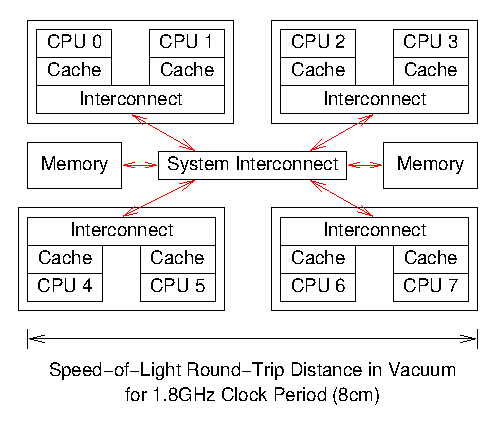
\includegraphics{cpu/SystemArch}}
\end{center}
\caption{System Hardware Architecture}
\label{fig:cpu:System Hardware Architecture}
\end{figure}

Figure~\ref{fig:cpu:System Hardware Architecture}
shows a rough schematic of an eight-core computer system.
Each die has a pair of CPU cores, each with its cache, as well as an
interconnect allowing the pair of CPUs to communicate with each other.
The system interconnect in the middle of the diagram allows the
four dies to communicate, and also connects them to main memory.

Data moves through this system in units of ``cache lines'', which
are power-of-two fixed-size aligned blocks of memory, usually ranging
from 32 to 256 bytes in size.
When a CPU loads a variable from memory to one of its registers, it must
first load the cacheline containing that variable into its cache.
Similarly, when a CPU stores a value from one of its registers into
memory, it must also load the cacheline containing that variable into
its cache, but must also ensure that no other CPU has a copy of that
cacheline.

For example, if CPU~0 were to perform a compare-and-swap (CAS) operation on a
variable whose cacheline resided in CPU~7's cache, the following
over-simplified sequence of events might ensue:

\begin{enumerate}
\item	CPU~0 checks its local cache, and does not find the cacheline.
\item	The request is forwarded to CPU~0's and 1's interconnect,
	which checks CPU~1's local cache, and does not find the cacheline.
\item	The request is forwarded to the system interconnect, which
	checks with the other three dies, learning that the cacheline
	is held by the die containing CPU~6 and 7.
\item	The request is forwarded to CPU~6's and 7's interconnect, which
	checks both CPUs' caches, finding the value in CPU~7's cache.
\item	CPU~7 forwards the cacheline to its interconnect, and also
	flushes the cacheline from its cache.
\item	CPU~6's and 7's interconnect forwards the cacheline to the
	system interconnect.
\item	The system interconnect forwards the cacheline to CPU~0's and 1's
	interconnect.
\item	CPU~0's and 1's interconnect forwards the cacheline to CPU~0's
	cache.
\item	CPU~0 can now perform the CAS operation on the value in its cache.
\end{enumerate}

\QuickQuiz{}
	This is a \emph{simplified} sequence of events?
	How could it \emph{possibly} be any more complex?
\QuickQuizAnswer{
	This sequence ignored a number of possible complications,
	including:

	\begin{enumerate}
	\item	Other CPUs might be concurrently attempting to perform
		CAS operations involving this same cacheline.
	\item	The cacheline might have been replicated read-only in
		several CPUs' caches, in which case, it would need to
		be flushed from their caches.
	\item	CPU~7 might have been operating on the cache line when
		the request for it arrived, in which case CPU~7 would
		need to hold of the request until its own operation
		completed.
	\item	CPU~7 might have ejected the cacheline from its cache
		(for example, in order to make room for other data),
		so that by the time that the request arrived, the
		cacheline was on its way to memory.
	\item	A correctable error might have occurred in the cacheline,
		which would then need to be corrected at some point before
		the data was used.
	\end{enumerate}

	Production-quality cache-coherence mechanisms are extremely
	complicated due to these sorts of considerations.

} \QuickQuizEnd

\QuickQuiz{}
	Why is it necessary to flush the cacheline from CPU~7's cache?
\QuickQuizAnswer{
	If the cacheline was not flushed from CPU~7's cache, then
	CPUs~0 and 7 might have different values for the same set
	of variables in the cacheline.
	This sort of incoherence would greatly complicate parallel
	software, and so hardware architects have been convinced to
	avoid it.
} \QuickQuizEnd

\subsection{Costs of Operations}
\label{sec:cpu:Costs of Operations}

\begin{table}
\centering
\begin{tabular}{l||r|r}
	Operation		& Cost (ns) 	& Ratio \\
	\hline
	\hline
	Clock period		&           0.6	&           1.0 \\
	\hline
	Best-case CAS		&          37.9	&          63.2 \\
	\hline
	Best-case lock		&          65.6	&         109.3\\
	\hline
	Single cache miss	&         139.5	&         232.5 \\
	\hline
	CAS cache miss		&         306.0	&         510.0 \\
	\hline
	Comms Fabric		&       3,000	&       5,000 \\
	\hline
	Global Comms		& 130,000,000	& 216,000,000 \\
\end{tabular}
\caption{Performance of Synchronization Mechanisms on 4-CPU 1.8GHz AMD Opteron 844 System}
\label{tab:cpu:Performance of Synchronization Mechanisms on 4-CPU 1.8GHz AMD Opteron 844 System}
\end{table}

The overheads of some common operations important to parallel programs are
displayed in
Table~\ref{tab:cpu:Performance of Synchronization Mechanisms on 4-CPU 1.8GHz AMD Opteron 844 System}.
This system's clock period rounds to 0.6ns.
Although it is not unusual for modern microprocessors to be able to retire
multiple instructions per clock period, the operations will be normalized
to a full clock period in the third column, labeled ``Ratio''.
The first thing to note about this table is the large values of many of
the ratios.

The best-case CAS operation consumes almost forty
nanoseconds, a duration more than sixty times that of the clock period.
Here, ``best case'' means that the same CPU now performing the CAS operation
on a given variable was the last CPU to operate on this variable, so
that the corresponding cache line is already held in that CPU's cache,
Similarly, the best-case lock operation (a ``round trip'' pair consisting
of a lock acquisition followed by a lock release) consumes more than
sixty nanosecond, or more than one hundred lock cycles.
Again, ``best case'' means that the data structure representing the
lock is already in the cache belonging to the CPU acquiring and releasing
the lock.
The lock operation is more expensive than CAS because it requires two
atomic operations on the lock data structure.

An operation that misses the cache consumes almost one hundred and forty
nanoseconds, or more than two hundred clock cycles.
A CAS operation, which must look at the old value of the variable as
well as store a new value, consumes over three hundred nanoseconds, or
more than five hundred clock cycles.
Think about this a bit.
In the time required to do \emph{one} CAS operation, the CPU could have
executed more than \emph{five hundred} normal instructions.
This should demonstrate the limitations of fine-grained locking.

\QuickQuiz{}
	Surely the hardware designers could be persuaded to improve
	this situation!
	Why have they been content with such abysmal performance
	for these single-instruction operations?
\QuickQuizAnswer{
	The hardware designers \emph{have} been working on this
	problem, and have consulted with no less a luminary than
	the physicist Stephen Hawking.
	Hawking's observation was that the hardware designers have
	two basic problems~\cite{BryanGardiner2007}:

	\begin{enumerate}
	\item	the finite speed of light, and
	\item	the atomic nature of matter.
	\end{enumerate}

\begin{table}
\centering
\begin{tabular}{l||r|r}
	Operation		& Cost (ns) 	& Ratio \\
	\hline
	\hline
	Clock period		&           0.4	&           1.0 \\
	\hline
	``Best-case'' CAS	&          12.2	&          33.8 \\
	\hline
	Best-case lock		&          25.6	&          71.2 \\
	\hline
	Single cache miss	&          12.9	&          35.8 \\
	\hline
	CAS cache miss		&           7.0	&          19.4 \\
	\hline
	Off-Core		&		&		\\
	\hline
	Single cache miss	&          31.2	&          86.6 \\
	\hline
	CAS cache miss		&          31.2	&          86.5 \\
	\hline
	Off-Socket		&		&		\\
	\hline
	Single cache miss	&          92.4	&         256.7 \\
	\hline
	CAS cache miss		&          95.9	&         266.4 \\
	\hline
	Comms Fabric		&       4,500	&       7,500 \\
	\hline
	Global Comms		& 195,000,000	& 324,000,000 \\
\end{tabular}
\caption{Performance of Synchronization Mechanisms on 16-CPU 2.8GHz Intel X5550 (Nehalem) System}
\label{tab:cpu:Performance of Synchronization Mechanisms on 16-CPU 2.8GHz Intel X5550 (Nehalem) System}
\end{table}

	The first problem limits raw speed, and the second limits
	miniaturization, which in turn limits frequency.
	And even this sidesteps the power-consumption issue that
	is currently holding production frequencies to well below
	10 GHz.

	Nevertheless, some progress is being made, as may be seen
	by comparing
	Table~\ref{tab:cpu:Performance of Synchronization Mechanisms on 16-CPU 2.8GHz Intel X5550 (Nehalem) System}
	with
	Table~\ref{tab:cpu:Performance of Synchronization Mechanisms on 4-CPU 1.8GHz AMD Opteron 844 System}
	on
	page~\ref{tab:cpu:Performance of Synchronization Mechanisms on 4-CPU 1.8GHz AMD Opteron 844 System}.
	Integration of hardware threads in a single core and multiple
	cores on a die have improved latencies greatly, at least within the
	confines of a single core or single die.
	There has been some improvement in overall system latency,
	but only by about a factor of two.
	Unfortunately, neither the speed of light nor the atomic nature
	of matter has changed much in the past few years.

	Section~\ref{sec:cpu:Hardware Free Lunch?}
	looks at what else hardware designers might be
	able to do to ease the plight of parallel programmers.
} \QuickQuizEnd

I/O operations are even more expensive.
A high performance (and expensive!) communications fabric, such as
InfiniBand or any number of proprietary interconnects, has a latency
of roughly three microseconds, during which time five \emph{thousand}
instructions might have been executed.
Standards-based communications networks often require some sort of
protocol processing, which further increases the latency.
Of course, geographic distance also increases latency, with the
theoretical speed-of-light latency around the world coming to
roughly 130 \emph{milliseconds}, or more than 200 million clock
cycles.

\QuickQuiz{}
	These numbers are insanely large!
	How can I possibly get my head around them?
\QuickQuizAnswer{
	Get a roll of toilet paper.
	In the USA, each roll will normally have somewhere around 350-500
	sheets.
	Tear off one sheet to represent a single clock cycle, setting it aside.
	Now unroll the rest of the roll.

	The resulting pile of toilet paper will likely represent a single
	CAS cache miss.

	For the more-expensive inter-system communications latencies,
	use several rolls (or multiple cases) of toilet paper to represent
	the communications latency.

	Important safety tip: make sure to account for the needs of
	those you live with when appropriating toilet paper!
} \QuickQuizEnd

% cpu/hwfreelunch.tex

\section{Hardware Free Lunch?}
\label{sec:cpu:Hardware Free Lunch?}

The major reason that concurrency has been receiving so much focus over
the past few years is the end of Moore's-Law induced single-threaded
performance increases
(or ``free lunch''~\cite{HerbSutter2008EffectiveConcurrency}),
as shown in
Figure~\ref{fig:intro:Clock-Frequency Trend for Intel CPUs} on
page~\pageref{fig:intro:Clock-Frequency Trend for Intel CPUs}.
This section briefly surveys a few ways that hardware designers
might be able to bring back some form of the ``free lunch''.

However, the preceding section presented some substantial hardware
obstacles to exploiting concurrency.
One severe physical limitation that hardware designers face is the
finite speed of light.
As noted in
Figure~\ref{fig:cpu:System Hardware Architecture} on
page~\pageref{fig:cpu:System Hardware Architecture},
light can travel only about an 8-centimeters round trip
in a vacuum during the duration of a 1.8 GHz clock period.
This distance drops to about 3 centimeters for a 5 GHz clock.
Both of these distances are relatively small compared to the size
of a modern computer system.

To make matters even worse, electrons in silicon move from three to
thirty times more slowly than does light in a vacuum, and common
clocked logic constructs run still more slowly, for example, a
memory reference may need to wait for a local cache lookup to complete
before the request may be passed on to the rest of the system.
Furthermore, relatively low speed and high power drivers are required
to move electrical signals from one silicon die to another, for example,
to communicate between a CPU and main memory.

There are nevertheless some technologies (both hardware and software)
that might help improve matters:

\begin{enumerate}
\item	3D integration,
\item	Novel materials and processes,
\item	Substituting light for electrons,
\item	Special-purpose accelerators, and
\item	Existing parallel software.
\end{enumerate}

Each of these is described in one of the following sections.

\subsection{3D Integration}
\label{sec:cpu:3D Integration}

3D integration is the practice of bonding very thin silicon dies to
each other in a vertical stack.
This practice provides potential benefits, but also poses
significant fabrication challenges~\cite{JohnKnickerbocker2008:3DI}.

\begin{figure}[tb]
\begin{center}
\resizebox{3in}{!}{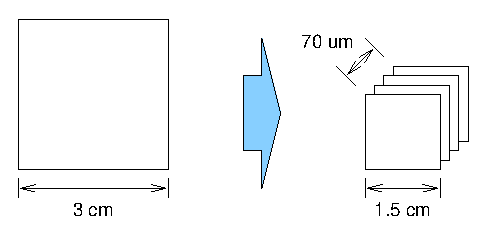
\includegraphics{cpu/3DI}}
\end{center}
\caption{Latency Benefit of 3D Integration}
\label{fig:cpu:Latency Benefit of 3D Integration}
\end{figure}

Perhaps the most important benefit of 3DI is decreased path length through
the system, as shown in
Figure~\ref{fig:cpu:Latency Benefit of 3D Integration}.
A 3-centimeter silicon die is replaced with a stack of four 1.5-centimeter
dies, in theory decreasing the maximum path through the system by a factor
of two, keeping in mind that each layer is quite thin.
In addition, given proper attention to design and placement,
long horizontal electrical connections (which are both slow and
power hungry) can be replaced by short vertical electrical connections,
which are both faster and more power efficient.

However, delays due to levels of clocked logic will not be decreased
by 3D integration, and significant manufacturing, testing, power-supply,
and heat-dissipation problems must be solved for 3D integration to
reach production while still delivering on its promise.
The heat-dissipation problems might be solved using
semiconductors based on diamond, which is a good conductor
for heat, but an electrical insulator.
That said, it remains difficult to grow large single diamond crystals,
to say nothing of slicing them into wafers.
In addition, it seems unlikely that any of these technologies will be able to
deliver the exponentially increases to which some people have become accustomed.
That said, they may be necessary steps on the path to the late Jim Gray's
``smoking hairy golf balls''~\cite{JimGray2002SmokingHairyGolfBalls}.

\subsection{Novel Materials and Processes}
\label{sec:cpu:Novel Materials and Processes}

Stephen Hawking is said to have claimed that semiconductor manufacturers
have but two fundamental problems: (1) the finite speed of light and
(2) the atomic nature of matter~\cite{BryanGardiner2007}.
It is possible that semiconductor manufacturers are approaching these
limits, but there are nevertheless a few avenues of research and
development focused on working around these fundamental limits.

One workaround for the atomic nature of matter are so-called
``high-K dielectric'' materials, which allow larger devices to mimic the
electrical properties of infeasibly small devices.
These materials pose some severe fabrication challenges, but nevertheless
may help push the frontiers out a bit farther.
Another more-exotic workaround stores multiple bits in a single electron,
relying on the fact that a given electron can exist at a number of
energy levels.
It remains to be seen if this particular approach can be made to work
reliably in production semiconductor devices.

Another proposed workaround is the ``quantum dot'' approach that
allows much smaller device sizes, but which is still in the research
stage.

Although the speed of light would be a hard limit, the fact is that
semiconductor devices are limited by the speed of electrons rather
than that of light, given that electrons in semiconductor materials
move at between 3\% and 30\% of the speed of light in a vacuum.
The use of copper connections on silicon devices is one way to increase
the speed of electrons, and it is quite possible that additional
advances will push closer still to the actual speed of light.
In addition, there have been some experiments with tiny optical fibers
as interconnects within and between chips, based on the fact that
the speed of light in glass is more than 60\% of the speed of light
in a vacuum.
One obstacle to such optical fibers is the inefficiency conversion
between electricity and light and vice versa, resulting in both
power-consumption and heat-dissipation problems.

That said, absent some fundamental advances in the field of physics,
any exponential increases in the speed of data flow
will be sharply limited by the actual speed of light in a vacuum.

\subsection{Special-Purpose Accelerators}
\label{sec:cpu:Special-Purpose Accelerators}

A general-purpose CPU working on a specialized problem is often spending
significant time and energy doing work that is only tangentially related
to the problem at hand.
For example, when taking the dot product of a pair of vectors, a
general-purpose CPU will normally use a loop (possibly unrolled)
with a loop counter.
Decoding the instructions, incrementing the loop counter, testing this
counter, and branching back to the
top of the loop are in some sense wasted effort: the real goal is
instead to multiply corresponding elements of the two vectors.
Therefore, a specialized piece of hardware designed specifically to
multiply vectors could get the job done more quickly and with less
energy consumed.

This is in fact the motivation for the vector instructions present in
many commodity microprocessors.
Because these instructions operate on multiple data items simultaneously,
they would permit a dot product to be computed with less instruction-decode
and loop overhead.

Similarly, specialized hardware can more efficiently encrypt and decrypt,
compress and decompress, encode and decode, and many other tasks besides.
Unfortunately, this efficiency does not come for free.
A computer system incorporating this specialized hardware will contain
more transistors, which will consume some power even when not in use.
Software must be modified to take advantage of this specialized hardware,
and this specialized hardware must be sufficiently generally useful
that the high up-front hardware-design costs can be spread over enough
users to make the specialized hardware affordable.
In part due to these sorts of economic considerations, specialized
hardware has thus far appeared only for a few application areas,
including graphics processing (GPUs), vector processors (MMX, SSE,
and VMX instructions), and, to a lesser extent, encryption.

Nevertheless, given the end of Moore's-Law-induced single-threaded
performance increases, it seems safe to predict that there will
be an increasing variety of special-purpose hardware going forward.

\subsection{Existing Parallel Software}
\label{sec:cpu:Existing Parallel Software}

Although multicore CPUs seem to have taken the computing industry
by surprise, the fact remains that shared-memory parallel computer
systems have been commercially available for more than a quarter
century.
This is more than enough time for significant parallel software
to make its appearance, and it indeed has.
Parallel operating systems are quite commonplace, as are parallel
threading libraries, parallel relational database management systems, 
and parallel numerical software are now readily available.
Using existing parallel software go a long ways towards solving any
parallel-software crisis we might encounter.

Perhaps the most common example is the parallel relational database
management system.
It is not unusual for single-threaded programs, often written in
high-level scripting languages, to access a central relational
database concurrently.
In the resulting highly parallel system, only the database need actually
deal directly with parallelism.
A very nice trick when it works!

% cpu/swdesign.tex

\section{Software Design Implications}
\label{sec:cpu:Software Design Implications}

The values of the ratios in
Table~\ref{tab:cpu:Performance of Synchronization Mechanisms on 4-CPU 1.8GHz AMD Opteron 844 System}
are critically important, as they limit the
efficiency of a given parallel application.
To see this, suppose that the parallel application uses CAS
operations to communicate among threads.
These CAS operations will typically involve a cache miss, that is, assuming
that the threads are communicating primarily with each other rather than
with themselves.
Suppose further that the unit of work corresponding to each CAS communication
operation takes 300ns, which is sufficient time to compute several
floating-point transcendental functions.
Then about half of the execution time will be consumed by the CAS
communication operations!
This in turn means that a two-CPU system running such a parallel program
would run no faster than one a sequential implementation running on a
single CPU.

The situation is even worse in the distributed-system case, where the
latency of a single communications operation might take as long as
thousands or even millions of floating-point operations.
This illustrates how important it is for communications operations to
be extremely infrequent and to enable very large quantities of processing.

\QuickQuiz{}
	Given that distributed-systems communication is so horribly
	expensive, why does anyone bother with them?
\QuickQuizAnswer{
	There are a number of reasons:

	\begin{enumerate}
	\item	Shared-memory multiprocessor systems have strict size limits.
		If you need more than a few thousand CPUs, you have no
		choice but to use a distributed system.
	\item	Extremely large shared-memory systems tend to be
		quite expensive and to have even longer cache-miss
		latencies than does the small four-CPU system
		shown in
		Table~\ref{tab:cpu:Performance of Synchronization Mechanisms on 4-CPU 1.8GHz AMD Opteron 844 System}.
	\item	The distributed-systems communications latencies do
		not necessarily consume the CPU, which can often allow
		computation to proceed in parallel with message transfer.
	\item	Many important problems are ``embarrassingly parallel'',
		so that extremely large quantities of processing may
		be enabled by a very small number of messages.
		SETI@HOME~\cite{SETIatHOME2008}
		is but one example of such an application.
		These sorts of applications can make good use of networks
		of computers despite extremely long communications
		latencies.
	\end{enumerate}

	It is likely that continued work on parallel applications will
	increase the number of embarrassingly parallel applications that
	can run well on machines and/or clusters having long communications
	latencies.
	That said, greatly reduced hardware latencies would be an
	extremely welcome development.
} \QuickQuizEnd

The lesson should be quite clear:
parallel algorithms must be explicitly designed
to run nearly independent threads.
The less frequently the threads communicate, whether by atomic operations,
locks, or explicit messages, the better the application's performance
and scalability will be.
In short, achieving excellent parallel performance and scalability means
striving for embarrassingly parallel algorithms and implementations,
whether by careful choice of data structures and algorithms, use of
existing parallel applications and environments, or transforming the
problem into one for which an embarrassingly parallel solution exists.

Chapter~\ref{cha:Partitioning and Synchronization Design}
will discuss design disciplines that promote performance and scalability.


% toolsoftrade/toolsoftrade.tex

\chapter{Tools of the Trade}
\label{chp:Tools of the Trade}

\QuickQuizChapter{chp:Tools of the Trade}

This chapter provides a brief introduction to some basic tools of the
parallel-programming trade, focusing mainly on those available to
user applications running on operating systems similar to Linux.
Section~\ref{sec:toolsoftrade:Scripting Languages} begins with
scripting languages,
Section~\ref{sec:toolsoftrade:POSIX Multiprocessing}
describes the multi-process parallelism supported by the POSIX API,
Section~\ref{sec:toolsoftrade:POSIX Multiprocessing} touches on POSIX threads,
and finally,
Section~\ref{sec:toolsoftrade:Atomic Operations}
describes atomic operations.

Please note that this chapter provides but a brief introduction.
More detail is available from the references cited, and more information
on how best to use these tools will be provided in later chapters.

\section{Scripting Languages}
\label{sec:toolsoftrade:Scripting Languages}

The Linux shell scripting languages provide simple but effective ways
of managing parallelism.
For example, suppose that you had a program \url{compute_it}
that you needed to run twice with two different sets of arguments.
This can be accomplished as follows:

\vspace{5pt}
\begin{minipage}[t]{\columnwidth}
\begin{verbatim}
  1 compute_it 1 > compute_it.1.out &
  2 compute_it 2 > compute_it.2.out &
  3 wait
  4 cat > compute_it.1.out
  5 cat > compute_it.2.out
\end{verbatim}
\end{minipage}
\vspace{5pt}

Lines~1 and 2 launch two instances of this program, redirecting their
output to two separate files, with the \url{&} character directing the
shell to run the two instances of the program in the background.
Line~3 waits for both instances to complete, and lines~4 and 5
display their output.
% @@@ Maui scheduler, load balancing, BOINC, and so on.

\QuickQuiz{}
	But these silly shell script isn't a \emph{real} parallel
	program!!!
	Why bother with such trivia???
\QuickQuizAnswer{
	Because you should \emph{never} forget the simple stuff!!!

	Please keep in mind that the title of this book is
	``Is Parallel Programming Hard, And, If So, What Can You Do About It?''.
	One of the most effective things you can do about it is to
	avoid forgetting the simple stuff!
	After all, if you choose to do parallel programming the hard
	way, you have no one but yourself to blame for it being hard.
} \QuickQuizEnd

For another example, the \url{make} software-build scripting language
provides a \url{-j} option that specifies how much parallelism should be
introduced into the build process.
For example, typing \url{make}~\url{-j4} when building a Linux kernel
specifies that up to four parallel compiles be carried out concurrently.

It is hoped that these simple examples convince you that parallel
programming need not always be complex or difficult.

\section{POSIX Multiprocessing}
\label{sec:toolsoftrade:POSIX Multiprocessing}

This section scratches the surface of the
POSIX pthreads~\cite{OpenGroup1997pthreads}
environment, as this environment is readily available and widely
implemented.
Section~\ref{sec:toolsoftrade:POSIX Thread Creation and Destruction}
touches on thread creation and distruction,
Section~\ref{sec:toolsoftrade:POSIX Locking} gives a brief overview
of POSIX locking, and, finally,
Section~\ref{sec:toolsoftrade:Linux-Kernel Equivalents to POSIX Operations}
presents the analogous operations within the Linux kernel.

\subsection{POSIX Thread Creation and Destruction}
\label{sec:toolsoftrade:POSIX Thread Creation and Destruction}

\url{pthread_create()}

\url{pthread_exit()}

\url{pthread_join()}

\subsection{POSIX Locking}
\label{sec:toolsoftrade:POSIX Locking}

\subsection{Linux-Kernel Equivalents to POSIX Operations}
\label{sec:toolsoftrade:Linux-Kernel Equivalents to POSIX Operations}

\section{Atomic Operations}
\label{sec:toolsoftrade:Atomic Operations}

% count/count.tex

\QuickQuizChapter{chp:Counting}{Counting}

Counting is perhaps the simplest and most natural for a computer to do.
However, counting efficiently and scalably on a large
shared-memory multiprocessor can be quite challenging.
Furthermore, the simplicity of the underlying concept of counting
allows us to explore the fundamental issues of concurrency without
the distractions
of elaborate data structures or complex synchronization primitives.
Counting therefore provides an excellent introduction to
parallel programming.

This chapter covers a number of special cases for which there are simple,
fast, and scalable counting algorithms.
But first, let us find out how much you already know about concurrent
counting.

\QuickQuiz{}
	Why on earth should efficient and scalable counting be hard?
	After all, computers have special hardware for the sole purpose
	of doing counting,
	addition, subtraction, and lots more besides, don't they???
\QuickQuizAnswer{
	Because the straightforward counting algorithms, for example,
	atomic operations on a shared counter, are slow and scale
	badly, as will be seen in
	Section~\ref{sec:count:Why Isn't Concurrent Counting Trivial?}.
} \QuickQuizEnd

\QuickQuiz{}
	{ \bfseries Network-packet counting problem. }
	Suppose that you need to collect statistics on the number
	of networking packets (or total number of bytes) transmitted
	and/or received.
	Packets might be transmitted or received by any CPU on
	the system.
	Suppose further that this large machine is capable of
	handling a million packets per second, and that there
	is a systems-monitoring package that reads out the count
	every five seconds.
	How would you implement this statistical counter?
\QuickQuizAnswer{
	Hint: the act of updating the counter must be blazingly
	fast, but because the counter is read out only about once
	in five million updates, the act of reading out the counter can be
	quite slow.
	In addition, the value read out normally need not be all that
	accurate---after all, since the counter is updated a thousand
	times per millisecond, we should be able to work with a value
	that is within a few thousand counts of the ``true value'',
	whatever ``true value'' might mean in this context.
	However, the value read out should maintain roughly the same
	absolute error over time.
	For example, a 1\% error might be just fine when the count
	is on the order of a million or so, but might be absolutely
	unacceptable once the count reaches a trillion.
	See Section~\ref{sec:count:Statistical Counters}.
} \QuickQuizEnd

\QuickQuiz{}
	{ \bfseries Approximate structure-allocation limit problem. }
	Suppose that you need to maintain a count of the number of
	structures allocated in order to fail any allocations
	once the number of structures in use exceeds a limit
	(say, 10,000).
	Suppose further that these structures are short-lived,
	that the limit is rarely exceeded, and that a ``sloppy''
	approximate limit is acceptable.
\QuickQuizAnswer{
	Hint: the act of updating the counter must be blazingly
	fast, but the counter is read out each time that the
	counter is increased.
	However, the value read out need not be accurate
	\emph{except} that it absolutely must distinguish perfectly
	between values below the limit and values greater than or
	equal to the limit.
	See Section~\ref{sec:count:Approximate Limit Counters}.
} \QuickQuizEnd

\QuickQuiz{}
	{ \bfseries Exact structure-allocation limit problem. }
	Suppose that you need to maintain a count of the number of
	structures allocated in order to fail any allocations
	once the number of structures in use exceeds an exact limit
	(say, 10,000).
	Suppose further that these structures are short-lived,
	and that the limit is rarely exceeded, that there is almost
	always at least one structure in use, and suppose further
	still that it is necessary to know exactly when this counter reaches
	zero, for example, in order to free up some memory
	that is not required unless there is at least one structure
	in use.
\QuickQuizAnswer{
	Hint: the act of updating the counter must be blazingly
	fast, but the counter is read out each time that the
	counter is increased.
	However, the value read out need not be accurate
	\emph{except} that it absolutely must distinguish perfectly
	between values between the limit and zero on the one hand,
	and values that either are less than or equal to zero or
	are greater than or equal to the limit on the other hand.
	See Section~\ref{sec:count:Exact Limit Counters}.
} \QuickQuizEnd

\QuickQuiz{}
	{ \bfseries Removable I/O device access-count problem. }
	Suppose that you need to maintain a reference count on a
	heavily used removable mass-storage device, so that you
	can tell the user when it is safe to removed the device.
	This device follows the usual removal procedure where
	the user indicates a desire to remove the device, and
	the system tells the user when it is safe to do so.
\QuickQuizAnswer{
	Hint: the act of updating the counter must be blazingly
	fast and scalable in order to avoid slowing down I/O operations,
	but because the counter is read out only when the
	user wishes to remove the device, the counter read-out
	operation can be extremely slow.
	Furthermore, there is no need to be able to read out
	the counter at all unless the user has already indicated
	a desire to remove the device.
	In addition, the value read out need not be accurate
	\emph{except} that it absolutely must distinguish perfectly
	between non-zero and zero values.
	However, once it has read out a zero value, it must act
	to keep the value at zero until it has taken some action
	to prevent subsequent threads from gaining access to the
	device being removed.
	See Section~\ref{sec:count:Applying Specialized Parallel Counters}.
} \QuickQuizEnd

The remainder of this chapter will develop answers to these questions.

\section{Why Isn't Concurrent Counting Trivial?}
\label{sec:count:Why Isn't Concurrent Counting Trivial?}

\begin{figure}[bp]
{ \scriptsize
\begin{verbatim}
  1 long counter = 0;
  2 
  3 void inc_count(void)
  4 {
  5   counter++;
  6 }
  7 
  8 long read_count(void)
  9 {
 10   return counter;
 11 }
\end{verbatim}
}
\caption{Just Count!}
\label{fig:count:Just Count!}
\end{figure}

Let's start with something simple, for example, the straightforward
use of arithmetic shown in
Figure~\ref{fig:count:Just Count!} (\url{count_nonatomic.c}).
Here, we have a counter on line~1, we increment it on line~5, and we
read out its value on line~10.
What could be simpler?

This approach has the additional advantage of being blazingly fast if
you are doing lots of reading and almost no incrementing, and on small
systems, the performance is excellent.

There is just one large fly in the ointment: this approach can lose
counts.
On my dual-core laptop, a short run invoked \co{inc_count()}
100,014,000 times, but the final value of the counter was only
52,909,118.
Although it is true that approximate values have their place in computing,
it is almost always necessary to do better than this.

\QuickQuiz{}
	But doesn't the \co{++} operator produce an x86 add-to-memory
	instruction?
	And won't the CPU cache cause this to be atomic?
\QuickQuizAnswer{
	Although the \co{++} operator \emph{could} be atomic, there
	is no requirement that it be so.
	Furthermore, the \co{ACCESS_ONCE()} primitive forces most
	version of {\sf gcc} to load the value to a register, increment
	the register, then store the value to memory, which is
	decidedly non-atomic.
} \QuickQuizEnd

\QuickQuiz{}
	The 8-figure accuracy on the number of failures indicates
	that you really did test this.
	Why would it be necessary to test such a trivial program,
	especially when the bug is easily seen by inspection?
\QuickQuizAnswer{
	There are no trivial parallel programs, and most days I am
	not so sure that there are trivial sequential programs, either.

	No matter how small or simple the program, if you haven't tested
	it, it does not work.
	And even if you have tested it, Murphy says there are at least a
	few bugs still lurking.

	Furthermore, while proofs of correctness certainly do have their
	place, they never will replace testing, including the
	\url{counttorture.h} test setup used here.
	After all, proofs can have bugs just as easily as programs can!
} \QuickQuizEnd

\begin{figure}[tbp]
{ \scriptsize
\begin{verbatim}
  1 atomic_t counter = ATOMIC_INIT(0);
  2 
  3 void inc_count(void)
  4 {
  5   atomic_inc(&counter);
  6 }
  7 
  8 long read_count(void)
  9 {
 10   return atomic_read(&counter);
 11 }
\end{verbatim}
}
\caption{Just Count Atomically!}
\label{fig:count:Just Count Atomically!}
\end{figure}

\begin{figure}[tb]
\begin{center}
\resizebox{3in}{!}{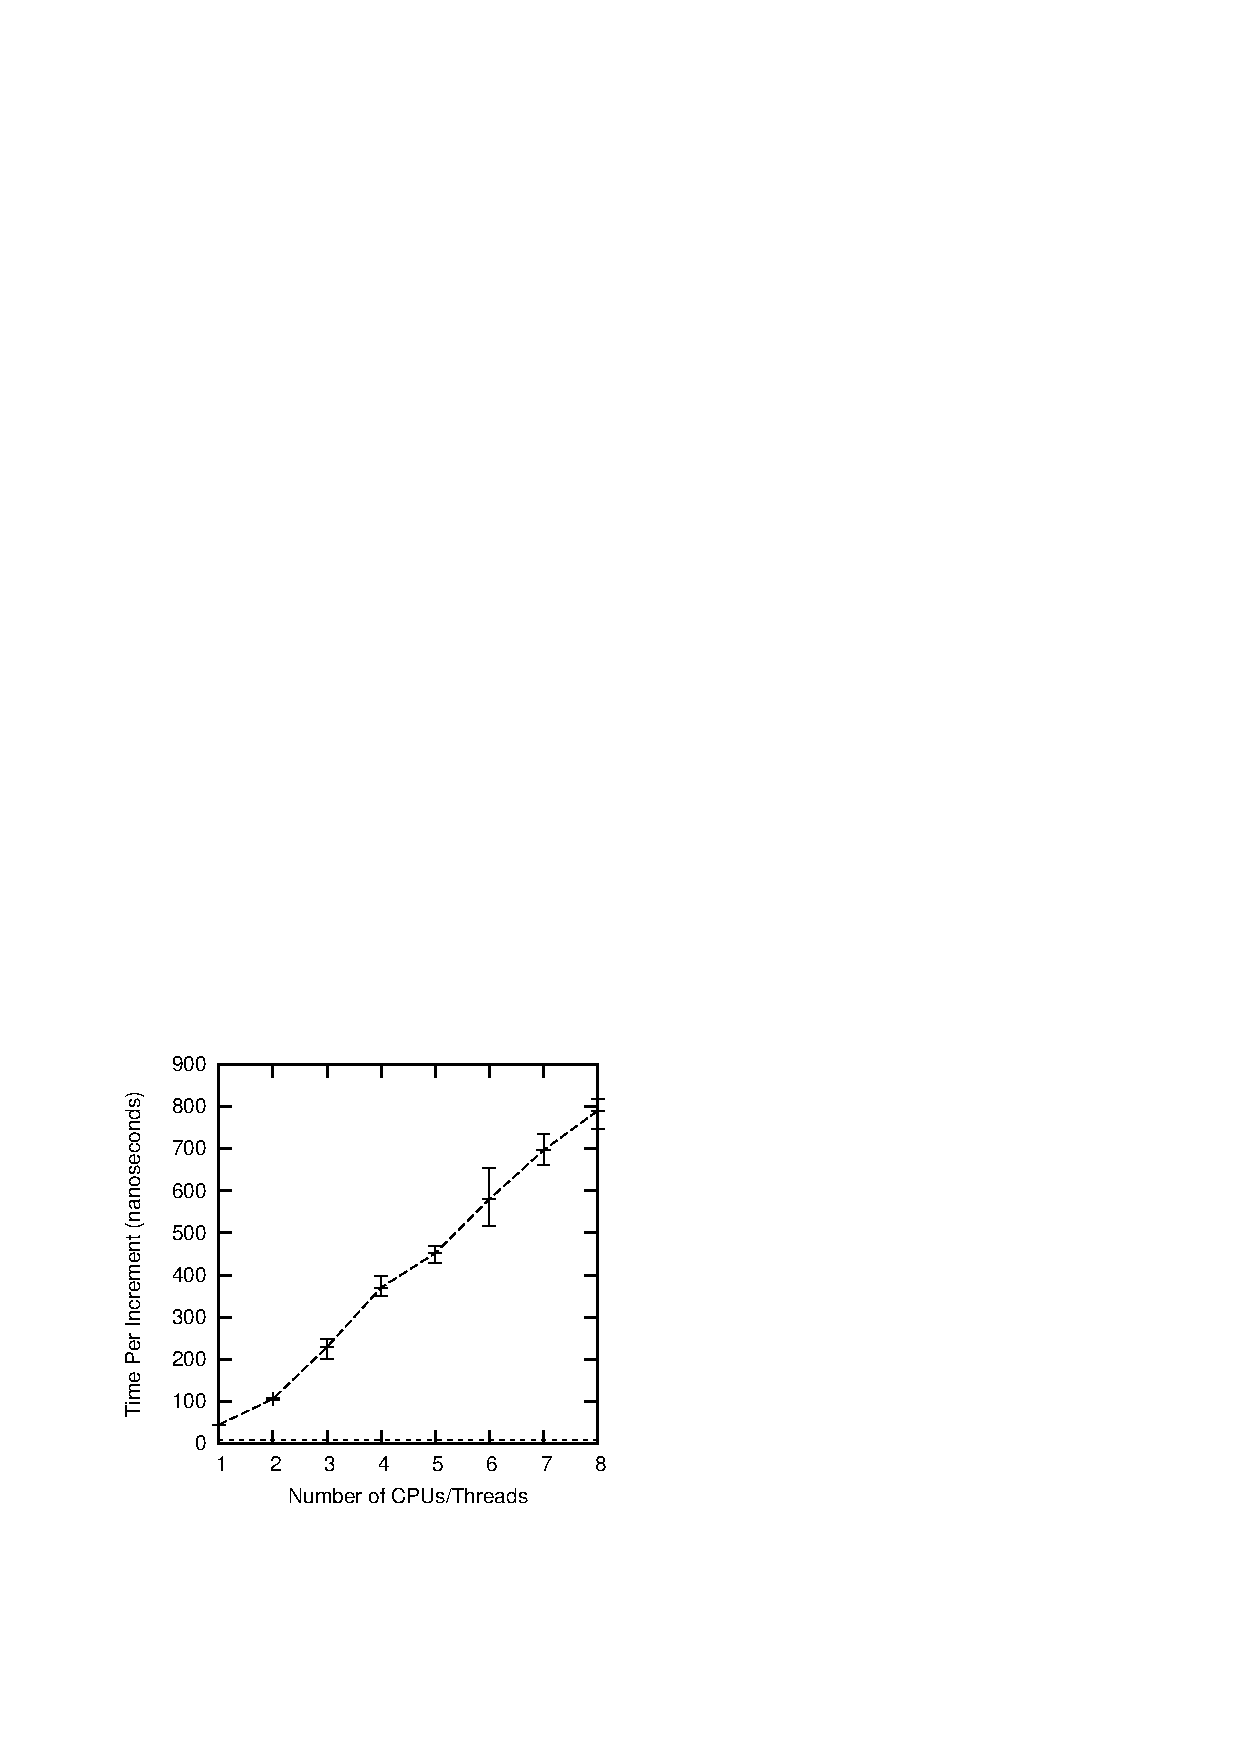
\includegraphics{CodeSamples/count/atomic}}
\end{center}
\caption{Atomic Increment Scalability on Nehalem}
\label{fig:count:Atomic Increment Scalability on Nehalem}
\end{figure}

The straightforward way to count accurately is to use atomic operations,
as shown in
Figure~\ref{fig:count:Just Count Atomically!} (\url{count_atomic.c}).
Line~1 defines an atomic variable, line~5 atomically increments it, and
line~10 reads it out.
Because this is atomic, it keeps perfect count.
However, it is slower: on a Intel Core Duo laptop, it is about
six times slower than non-atomic increment
when a single thread is incrementing, and more than \emph{ten times}
slower if two threads are incrementing.\footnote{
	Interestingly enough, a pair of threads non-atomically incrementing
	a counter will cause the counter to increase more quickly than
	a pair of threads atomically incrementing the counter.
	Of course, if your only goal is to make the counter increase
	quickly, an easier approach is to simply assign a large value
	to the counter.
	Nevertheless, there is likely to be a role for algorithms that
	use carefully relaxed notions of correctness in order to gain
	greater performance and
	scalability~\cite{Andrews91textbook,Arcangeli03,DavidUngar2011unsync}.}

This poor performance should not be a surprise, given the discussion in
Chapter~\ref{chp:Hardware and its Habits},
nor should it be a surprise that the performance of atomic increment
gets slower as the number of CPUs and threads increase, as shown in
Figure~\ref{fig:count:Atomic Increment Scalability on Nehalem}.
In this figure, the horizontal dashed line resting on the x~axis
is the ideal performance that would be achieved
by a perfectly scalable algorithm: with such an algorithm, a given
increment would incur the same overhead that it would in a single-threaded
program.
Atomic increment of a single global variable is clearly
decidedly non-ideal, and gets worse as you add CPUs.

\QuickQuiz{}
	Why doesn't the dashed line on the x~axis meet the 
	diagonal line at $y=1$?
\QuickQuizAnswer{
	Because of the overhead of the atomic operation.
	The dashed line on the x~axis represents the overhead of
	a single \emph{non-atomic} increment.
	After all, an \emph{ideal} algorithm would not only scale
	linearly, it would also incur no performance penalty compared
	to single-threaded code.

	This level of idealism may seem severe, but if it is good
	enough for Linus Torvalds, it is good enough for you.
} \QuickQuizEnd

\QuickQuiz{}
	But atomic increment is still pretty fast.
	And incrementing a single variable in a tight loop sounds
	pretty unrealistic to me, after all, most of the program's
	execution should be devoted to actually doing work, not accounting
	for the work it has done!
	Why should I care about making this go faster?
\QuickQuizAnswer{
	In many cases, atomic increment will in fact be fast enough
	for you.
	In those cases, you should by all means use atomic increment.
	That said, there are many real-world situations where
	more elaborate counting algorithms are required.
	The canonical example of such a situation is counting packets
	and bytes in highly optimized networking stacks, where it is
	all too easy to find much of the execution time going into
	these sorts of accounting tasks, especially on large
	multiprocessors.

	In addition, counting provides an excellent view of the
	issues encountered in shared-memory parallel programs.
} \QuickQuizEnd

\begin{figure}[tb]
\begin{center}
\resizebox{3in}{!}{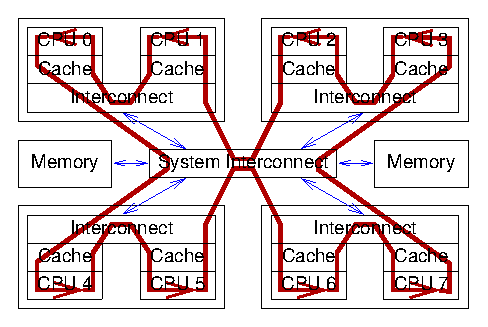
\includegraphics{count/GlobalInc}}
\end{center}
\caption{Data Flow For Global Atomic Increment}
\label{fig:count:Data Flow For Global Atomic Increment}
\end{figure}

For another perspective on global atomic increment, consider
Figure~\ref{fig:count:Data Flow For Global Atomic Increment}.
In order for each CPU to get a chance to increment a given
global variable, the cache line containing that variable must
circulate among all the CPUs, as shown by the red arrows.
Such circulation will take significant time, resulting in
the poor performance seen in
Figure~\ref{fig:count:Atomic Increment Scalability on Nehalem}.

The following sections discuss high-performance counting, which
avoids the delays inherent in such circulation.

\QuickQuiz{}
	But why can't CPU designers simply ship the operation to the
	data, avoiding the need to circulate the cache line containing
	the global variable being incremented?
\QuickQuizAnswer{
	It might well be possible to do this in some cases.
	However, there are a few complications:
	\begin{enumerate}
	\item	If the value of the variable is required, then the
		thread will be forced to wait for the operation
		to be shipped to the data, and then for the result
		to be shipped back.
	\item	If the atomic increment must be ordered with respect
		to prior and/or subsequent operations, then the thread
		will be forced to wait for the operation to be shipped
		to the data, and for an indication that the operation
		completed to be shipped back.
	\item	Shipping operations among CPUs will likely require
		more signals, which will consume more die area and
		more electrical power.
	\end{enumerate}
	But what if neither of the first two conditions holds?
	Then you should think carefully about the algorithms discussed
	in Section~\ref{sec:count:Statistical Counters}, which achieve
	near-ideal performance on commodity hardware.

\begin{figure}[tb]
\begin{center}
\resizebox{3in}{!}{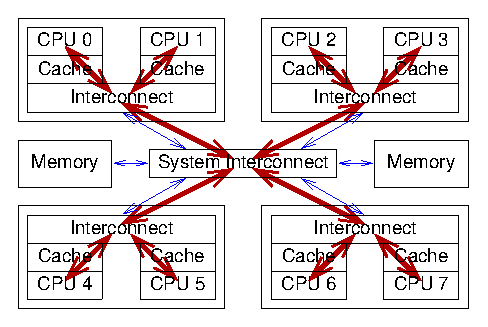
\includegraphics{count/GlobalTreeInc}}
\end{center}
\caption{Data Flow For Global Combining-Tree Atomic Increment}
\label{fig:count:Data Flow For Global Combining-Tree Atomic Increment}
\end{figure}

	If either or both of the first two conditions hold, there is
	\emph{some} hope for improvement.
	One could imagine the hardware implementing a combining tree,
	so that the increment requests from multiple CPUs are combined
	by the hardware into a single addition when the combined request
	reaches the hardware.
	The hardware could also apply an order to the requests, thus
	returning to each CPU the return value corresponding to its
	particular atomic increment.
	This results in instruction latency that varies as $O(log N)$,
	where $N$ is the number of CPUs, as shown in
	Figure~\ref{fig:count:Data Flow For Global Combining-Tree Atomic Increment}.
	And CPUs with this sort of hardware optimization are starting to
	appear as of 2011.

	This is a great improvement over the $O(N)$ performance
	of current hardware shown in
	Figure~\ref{fig:count:Data Flow For Global Atomic Increment},
	and it is possible that hardware latencies might decrease
	further if innovations such as three-D fabrication prove
	practical.
	Nevertheless, we will see that in some important special cases,
	software can do \emph{much} better.
} \QuickQuizEnd

\section{Statistical Counters}
\label{sec:count:Statistical Counters}

This section covers the common special case of statistical counters, where
the count is updated extremely frequently and the value is read out
rarely, if ever.
These will be used to solve the network-packet counting problem
from the Quick Quiz on
page~\pageref{chp:Counting}.

\subsection{Design}

Statistical counting is typically handled by providing a counter per
thread (or CPU, when running in the kernel), so that each thread
updates its own counter.
The aggregate value of the counters is read out by simply summing up
all of the threads' counters,
relying on the commutative and associative properties of addition.
This is an example of the Data Ownership pattern that will be introduced in
Section~\ref{sec:SMPdesign:Data Ownership}.

\QuickQuiz{}
	But doesn't the fact that C's ``integers'' are limited in size
	complicate things?
\QuickQuizAnswer{
	No, because modulo addition is still commutative and associative.
	At least as long as you use unsigned integer.
	Recall that in the C standard, overflow of signed integers results
	in undefined behavior (never mind the fact that machines that
	do anything other than wrap on overflow are quite rare these days.

	That said, one potential source of additional complexity arises
	when attempting to gather (say) a 64-bit sum from 32-bit
	per-thread counters.
	For the moment, dealing with this added complexity is left as
	an exercise for the reader.
} \QuickQuizEnd

\subsection{Array-Based Implementation}
\label{sec:count:Array-Based Implementation}

One way to provide per-thread variables is to allocate an array with
one element per
thread (presumably cache aligned and padded to avoid false sharing).

\QuickQuiz{}
	An array???
	But doesn't that limit the number of threads?
\QuickQuizAnswer{
	It can, and in this toy implementation, it does.
	But it is not that hard to come up with an alternative
	implementation that permits an arbitrary number of threads.
	However, this is left as an exercise for the reader.
} \QuickQuizEnd

\begin{figure}[tbp]
{ \scriptsize
\begin{verbatim}
  1 DEFINE_PER_THREAD(long, counter);
  2 
  3 void inc_count(void)
  4 {
  5   __get_thread_var(counter)++;
  6 }
  7 
  8 long read_count(void)
  9 {
 10   int t;
 11   long sum = 0;
 12 
 13   for_each_thread(t)
 14     sum += per_thread(counter, t);
 15   return sum;
 16 }
\end{verbatim}
}
\caption{Array-Based Per-Thread Statistical Counters}
\label{fig:count:Array-Based Per-Thread Statistical Counters}
\end{figure}

Such an array can be wrapped into per-thread primitives, as shown in
Figure~\ref{fig:count:Array-Based Per-Thread Statistical Counters}
(\url{count_stat.c}).
Line~1 defines an array containing a set of per-thread counters of
type \co{long} named, creatively enough, \co{counter}.

Lines~3-6 show a function that increments the counters, using the
\co{__get_thread_var()} primitive to locate the currently running
thread's element of the \co{counter} array.
Because this element is modified only by the corresponding thread,
non-atomic increment suffices.

Lines~8-16 show a function that reads out the aggregate value of the counter,
using the \co{for_each_thread()} primitive to iterate over the list of
currently running threads, and using the \co{per_thread()} primitive
to fetch the specified thread's counter.
Because the hardware can fetch and store a properly aligned \co{long}
atomically, and because gcc is kind enough to make use of this capability,
normal loads suffice, and no special atomic instructions are required.

\QuickQuiz{}
	What other choice does gcc have, anyway???
\QuickQuizAnswer{
	According to the C standard, the effects of fetching a variable
	that might be concurrently modified by some other thread are
	undefined.
	It turns out that the C standard really has no other choice,
	given that C must support (for example) eight-bit architectures
	which are incapable of atomically loading a \co{long}.
	An upcoming version of the C standard aims to fill this gap,
	but until then, we depend on the kindness of the gcc developers.
} \QuickQuizEnd

\QuickQuiz{}
	How does the per-thread \co{counter} variable in
	Figure~\ref{fig:count:Array-Based Per-Thread Statistical Counters}
	get initialized?
\QuickQuizAnswer{
	The C standard specifies that the initial value of
	global variables is zero, unless they are explicitly initialized.
	So the initial value of all the instances of \co{counter}
	will be zero.

	That said, one often takes differences of consecutive reads
	from statistical counters, in which case the initial value
	is irrelevant.
} \QuickQuizEnd

\QuickQuiz{}
	How is the code in
	Figure~\ref{fig:count:Array-Based Per-Thread Statistical Counters}
	supposed to permit more than one counter?
\QuickQuizAnswer{
	Indeed, this toy example does not support more than one counter.
	Modifying it so that it can provide multiple counters is left
	as an exercise to the reader.
} \QuickQuizEnd

\begin{figure}[tb]
\begin{center}
\resizebox{3in}{!}{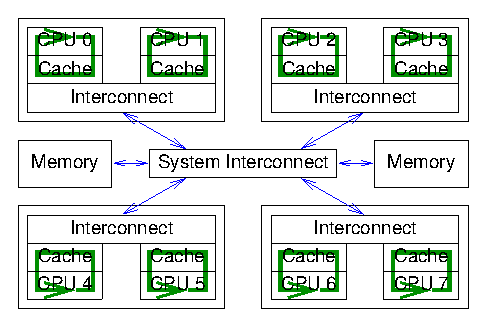
\includegraphics{count/PerThreadInc}}
\end{center}
\caption{Data Flow For Per-Thread Increment}
\label{fig:count:Data Flow For Per-Thread Increment}
\end{figure}

This approach scales linearly with increasing number of updater threads
invoking \co{inc_count()}.
As is shown by the green arrows in
Figure~\ref{fig:count:Data Flow For Per-Thread Increment},
the reason for this is that each CPU can make rapid progress incrementing
its thread's variable, with no expensive communication required crossing
the full diameter of the computer system.
However, this excellent update-side scalability comes at great read-side
expense for large numbers of threads.
The next section shows one way to reduce read-side expense while
still retaining the update-side scalability.

\subsection{Eventually Consistent Implementation}
\label{sec:count:Eventually Consistent Implementation}

One way to retain update-side scalability while greatly improving
read-side performance is to weaken consistency requirements.
While the counting algorithm in the previous section is guaranteed to
return a value between the value that an ideal counter would have
taken on near the beginning of \co{read_count()}'s execution and
that near the end of \co{read_count()}'s execution.
\emph{Eventual consistency}~\cite{WernerVogels:2009:EventuallyConsistent}
provides a weaker
guarantee: in absence of calls to \co{inc_count()}, calls to
\co{read_count()} will eventually return the correct answer.

We exploit eventual consistency by maintaining a global counter.
However, updaters only manipulate their per-thread counters.
A separate thread is provided to transfer counts from the per-thread
counters to the global counter.
Readers simply access the value of the global counter.
If updaters are active, the value used by the readers will be out of
date, however, once updates cease, the global counter will eventually
converge on the true value---hence this approach qualifies as
eventually consistent.

\begin{figure}[tbp]
{ \scriptsize
\begin{verbatim}
  1 DEFINE_PER_THREAD(unsigned long, counter);
  2 unsigned long global_count;
  3 int stopflag;
  4 
  5 void inc_count(void)
  6 {
  7   ACCESS_ONCE(__get_thread_var(counter))++;
  8 }
  9 
 10 unsigned long read_count(void)
 11 {
 12   return global_count;
 13 }
 14 
 15 void *eventual(void *arg)
 16 {
 17   int t;
 18   int sum;
 19 
 20   while (stopflag < 3) {
 21     sum = 0;
 22     for_each_thread(t)
 23       sum += per_thread(counter, t);
 24     ACCESS_ONCE(global_count) = sum;
 25     poll(NULL, 0, 1);
 26     if (stopflag) {
 27       smp_mb();
 28       stopflag++;
 29     }
 30   }
 31   return NULL;
 32 }
 33 
 34 void count_init(void)
 35 {
 36   thread_id_t tid;
 37 
 38   if (pthread_create(&tid, NULL, eventual, NULL) != 0) {
 39     perror("count_init:pthread_create");
 40     exit(-1);
 41   }
 42 }
 43 
 44 void count_cleanup(void)
 45 {
 46   stopflag = 1;
 47   while (stopflag < 3)
 48     poll(NULL, 0, 1);
 49   smp_mb();
 50 }
\end{verbatim}
}
\caption{Array-Based Per-Thread Eventually Consistent Counters}
\label{fig:count:Array-Based Per-Thread Eventually Consistent Counters}
\end{figure}

The implementation is shown in
Figure~\ref{fig:count:Array-Based Per-Thread Eventually Consistent Counters}
(\url{count_stat_eventual.c}).
Lines~1-2 show the per-thread variable and the global variable that
track the counter's value, and line three shows \co{stopflag}
which is used to coordinate termination (for the case where we want
to terminate the program with an accurate counter value).
The \co{inc_count()} function shown on lines~5-8 is similar to its
counterpart in
Figure~\ref{fig:count:Array-Based Per-Thread Statistical Counters}.
The \co{read_count()} function shown on lines~10-13 simply returns the
value of the \co{global_count} variable.

However, the \co{count_init()} function on lines~34-42
creates the \co{eventual()} thread shown on lines~15-32, which
cycles through all the threads,
summing the per-thread local \co{counter} and storing the
sum to the \co{global_count} variable.
The \co{eventual()} thread waits an arbitrarily chosen one millisecond
between passes.
The \co{count_cleanup()} function on lines~44-50 coordinates termination.

This approach gives extremely fast counter read-out while still
supporting linear counter-update performance.
However, this excellent read-side performance and update-side scalability
comes at the cost of the additional thread running \co{eventual()}.

\QuickQuiz{}
	Why doesn't \co{inc_count()} in
	Figure~\ref{fig:count:Array-Based Per-Thread Eventually Consistent Counters}
	need to use atomic instructions?
	After all, we now have multiple threads accessing the per-thread
	counters!
\QuickQuizAnswer{
	Because one of the two threads only reads, and because the
	variable is aligned and machine-sized, non-atomic instructions
	suffice.
	That said, the \co{ACCESS_ONCE()} macro is used to prevent
	compiler optimizations that might otherwise prevent the
	counter updates from becoming visible to
	\co{eventual()}~\cite{JonCorbet2012ACCESS:ONCE}.

	An older version of this algorithm did in fact use atomic
	instructions, kudos to Ersoy Bayramoglu for pointing out that
	they are in fact unnecessary.
	That said, atomic instructions would be needed in cases where
	the per-thread \co{counter} variables were smaller than the
	global \co{global_count}.
	For example, on a 32-bit system, the per-thread \co{counter} variables
	might need to be limited to 32 bits in order to sum them accurately,
	but a 64-bit \co{global_count} variable.
	In this case, it is necessary to zero the per-thead
	\co{counter} variables periodically in order to avoid
	overflow.
	In contrast, if all variables are the same size, overflow
	of any variable is harmless because the eventual sum
	will be modulo the word size.
} \QuickQuizEnd

\QuickQuiz{}
	Won't the single global thread in the function \co{eventual()} of
	Figure~\ref{fig:count:Array-Based Per-Thread Eventually Consistent Counters}
	be just as severe a bottleneck as a global lock would be?
\QuickQuizAnswer{
	In this case, no.
	What will happen instead is that the estimate of the counter
	value returned by \co{read_count()} will become more inaccurate.
} \QuickQuizEnd

\QuickQuiz{}
	Won't the estimate returned by \co{read_count()} in
	Figure~\ref{fig:count:Array-Based Per-Thread Eventually Consistent Counters}
	become increasingly
	inaccurate as the number of threads rises?
\QuickQuizAnswer{
	Yes.
	If this proves problematic, one fix is to provide multiple
	\co{eventual()} threads, each covering its own subset of
	the other threads.
	In even more extreme cases, a tree-like hierarchy of
	\co{eventual()} threads might be required.
} \QuickQuizEnd

\subsection{Per-Thread-Variable-Based Implementation}
\label{sec:count:Per-Thread-Variable-Based Implementation}

\begin{figure}[tbp]
{ \scriptsize
\begin{verbatim}
  1 long __thread counter = 0;
  2 long *counterp[NR_THREADS] = { NULL };
  3 long finalcount = 0;
  4 DEFINE_SPINLOCK(final_mutex);
  5 
  6 void inc_count(void)
  7 {
  8   counter++;
  9 }
 10 
 11 long read_count(void)
 12 {
 13   int t;
 14   long sum;
 15 
 16   spin_lock(&final_mutex);
 17   sum = finalcount;
 18   for_each_thread(t)
 19     if (counterp[t] != NULL)
 20       sum += *counterp[t];
 21   spin_unlock(&final_mutex);
 22   return sum;
 23 }
 24 
 25 void count_register_thread(void)
 26 {
 27   int idx = smp_thread_id();
 28 
 29   spin_lock(&final_mutex);
 30   counterp[idx] = &counter;
 31   spin_unlock(&final_mutex);
 32 }
 33 
 34 void count_unregister_thread(int nthreadsexpected)
 35 {
 36   int idx = smp_thread_id();
 37 
 38   spin_lock(&final_mutex);
 39   finalcount += counter;
 40   counterp[idx] = NULL;
 41   spin_unlock(&final_mutex);
 42 }
\end{verbatim}
}
\caption{Per-Thread Statistical Counters}
\label{fig:count:Per-Thread Statistical Counters}
\end{figure}

Fortunately, gcc provides an \co{__thread} storage class that provides
per-thread storage.
This can be used as shown in
Figure~\ref{fig:count:Per-Thread Statistical Counters} (\url{count_end.c})
to implement
a statistical counter that not only scales, but that also incurs little
or no performance penalty to incrementers compared to simple non-atomic
increment.

Lines~1-4 define needed variables: \co{counter} is the per-thread counter
variable, the \co{counterp[]} array allows threads to access each others'
counters, finalcount accumulates the total as individual threads exit,
and \co{final_mutex} coordinates between threads accumulating the total
value of the counter and exiting threads.

\QuickQuiz{}
	Why do we need an explicit array to find the other threads'
	counters?
	Why doesn't gcc provide a \co{per_thread()} interface, similar
	to the Linux kernel's \co{per_cpu()} primitive, to allow
	threads to more easily access each others' per-thread variables?
\QuickQuizAnswer{
	Why indeed?

	To be fair, gcc faces some challenges that the Linux kernel
	gets to ignore.
	When a user-level thread exits, its per-thread variables all
	disappear, which complicates the problem of per-thread-variable
	access, particularly before the advent of user-level RCU.
	In contrast, in the Linux kernel, when a CPU goes offline,
	that CPU's per-CPU variables remain mapped and accessible.

	Similarly, when a new user-level thread is created, its
	per-thread variables suddenly come into existence.
	In contrast, in the Linux kernel, all per-CPU variables are
	mapped and initialized at boot time, regardless of whether
	the corresponding CPU exists yet, or indeed, whether the
	corresponding CPU will ever exist.

	A key limitation that the Linux kernel imposes is a compile-time
	maximum limit on the number of CPUs, namely,
	\co{CONFIG_NR_CPUS}.
	In contrast, in user space, there is no hard-coded upper limit
	on the number of threads.

	Of course, both environments must deal with dynamically loaded
	code (dynamic libraries in user space, kernel modules in the
	Linux kernel), which increases the complexity of per-thread
	variables in both environments.

	These complications make it significantly harder for user-space
	environments to provide access to other threads' per-thread
	variables.
	Nevertheless, such access is highly useful, and it is hoped
	that it will someday appear.
} \QuickQuizEnd

The \co{inc_count()} function used by updaters is quite simple, as can
be seen on lines~6-9.

The \co{read_count()} function used by readers is a bit more complex.
Line~16 acquires a lock to exclude exiting threads, and line~21 releases
it.
Line~17 initializes the sum to the count accumulated by those threads that
have already exited, and lines~18-20 sum the counts being accumulated
by threads currently running.
Finally, line~22 returns the sum.

\QuickQuiz{}
	Why on earth do we need something as heavyweight as a \emph{lock}
	guarding the summation in the function \co{read_count()} in
	Figure~\ref{fig:count:Per-Thread Statistical Counters}?
\QuickQuizAnswer{
	Remember, when a thread exits, its per-thread variables disappear.
	Therefore, if we attempt to access a given thread's per-thread
	variables after that thread exits, we will get a segmentation
	fault.
	The lock coordinates summation and thread exit, preventing this
	scenario.

	Of course, we could instead read-acquire a reader-writer lock,
	but Chapter~\ref{chp:Deferred Processing} will introduce even
	lighter-weight mechanisms for implementing the required coordination.
} \QuickQuizEnd

Lines~25-32 show the \co{count_register_thread()} function, which
must be called by each thread before its first use of this counter.
This function simply sets up this thread's element of the \co{counterp[]}
array to point to its per-thread \co{counter} variable.

\QuickQuiz{}
	Why on earth do we need to acquire the lock in
	\co{count_register_thread()} in
	Figure~\ref{fig:count:Per-Thread Statistical Counters}?
	It is a single properly aligned machine-word store to a location
	that no other thread is modifying, so it should be atomic anyway,
	right?
\QuickQuizAnswer{
	This lock could in fact be omitted, but better safe than
	sorry, especially given that this function is executed only at
	thread startup, and is therefore not on any critical path.
	Now, if we were testing on machines with thousands of CPUs,
	we might need to omit the lock, but on machines with ``only''
	a hundred or so CPUs, no need to get fancy.
} \QuickQuizEnd

Lines~34-42 show the \co{count_unregister_thread()} function, which
must be called prior to exit by each thread that previously called
\co{count_register_thread()}.
Line~38 acquires the lock, and line~41 releases it, thus excluding any
calls to \co{read_count()} as well as other calls to
\co{count_unregister_thread()}.
Line~39 adds this thread's \co{counter} to the global \co{finalcount},
and then \co{NULL}s out its \co{counterp[]} array entry.
A subsequent call to \co{read_count()} will see the exiting thread's
count in the global \co{finalcount}, and will skip the exiting thread
when sequencing through the \co{counterp[]} array, thus obtaining
the correct total.

This approach gives updaters almost exactly the same performance as
a non-atomic add, and also scales linearly.
On the other hand, concurrent reads contend for a single global lock,
and therefore perform poorly and scale abysmally.
However, this is not a problem for statistical counters, where incrementing
happens often and readout happens almost never.
In addition, this approach is considerably more complex than the
array-based scheme, due to the fact that a given thread's per-thread
variables vanish when that thread exits.

\QuickQuiz{}
	Fine, but the Linux kernel doesn't have to acquire a lock
	when reading out the aggregate value of per-CPU counters.
	So why should user-space code need to do this???
\QuickQuizAnswer{
	Remember, the Linux kernel's per-CPU variables are always
	accessible, even if the corresponding CPU is offline --- even
	if the corresponding CPU never existed and never will exist.

\begin{figure}[tbp]
{ \scriptsize
\begin{verbatim}
  1 long __thread counter = 0;
  2 long *counterp[NR_THREADS] = { NULL };
  3 int finalthreadcount = 0;
  4 DEFINE_SPINLOCK(final_mutex);
  5 
  6 void inc_count(void)
  7 {
  8   counter++;
  9 }
 10 
 11 long read_count(void)
 12 {
 13   int t;
 14   long sum = 0;
 15 
 16   for_each_thread(t)
 17     if (counterp[t] != NULL)
 18       sum += *counterp[t];
 19   return sum;
 20 }
 21 
 22 void count_init(void)
 23 {
 24 }
 25 
 26 void count_register_thread(void)
 27 {
 28   counterp[smp_thread_id()] = &counter;
 29 }
 30 
 31 void count_unregister_thread(int nthreadsexpected)
 32 {
 33   spin_lock(&final_mutex);
 34   finalthreadcount++;
 35   spin_unlock(&final_mutex);
 36   while (finalthreadcount < nthreadsexpected)
 37     poll(NULL, 0, 1);
 38 }
\end{verbatim}
}
\caption{Per-Thread Statistical Counters With Lockless Summation}
\label{fig:count:Per-Thread Statistical Counters With Lockless Summation}
\end{figure}

	One workaround is to ensure that each thread sticks around
	until all threads are finished, as shown in
	Figure~\ref{fig:count:Per-Thread Statistical Counters With Lockless Summation}.
	Analysis of this code is left as an exercise to the reader,
	however, please note that it does not fit well into the
	\url{counttorture.h} counter-evaluation scheme.
	(Why not?)
	Chapter~\ref{chp:Deferred Processing} will introduce 
	synchronization mechanisms that handle this situation in a much
	more graceful manner.
} \QuickQuizEnd

\subsection{Discussion}

These two implementations show that it is possible to obtain uniprocessor
performance for statistical counters, despite running on a parallel
machine.

\QuickQuiz{}
	What fundamental difference is there between counting packets
	and counting the total number of bytes in the packets, given
	that the packets vary in size?
\QuickQuizAnswer{
	When counting packets, the counter is only incremented by the
	value one.
	On the other hand, when counting bytes, the counter might
	be incremented by largish numbers.

	Why does this matter?
	Because in the increment-by-one case, the value returned will
	be exact in the sense that the counter must necessarily have
	taken on that value at some point in time, even if it is impossible
	to say precisely when that point occurred.
	In contrast, when counting bytes, two different threads might
	return values that are inconsistent with any global ordering
	of operations.

	To see this, suppose that thread~0 adds the value three to its
	counter, thread~1 adds the value five to its counter, and
	threads~2 and 3 sum the counters.
	If the system is ``weakly ordered'' or if the compiler
	uses aggressive optimizations, thread~2 might find the
	sum to be three and thread~3 might find the sum to be five.
	The only possible global orders of the sequence of values
	of the counter are 0,3,8 and 0,5,8, and neither order is
	consistent with the results obtained.

	If you missed this one, you are not alone.
	Michael Scott used this question to stump Paul McKenney during Paul's
	Ph.D. defense.
} \QuickQuizEnd

\QuickQuiz{}
	Given that the reader must sum all the threads' counters,
	this could take a long time given large numbers of threads.
	Is there any way that the increment operation can remain
	fast and scalable while allowing readers to also enjoy
	reasonable performance and scalability?
\QuickQuizAnswer{
	One approach would be to maintain a global approximation
	to the value.
	Readers would increment their per-thread variable, but when it
	reached some predefined limit, atomically add it to a global
	variable, then zero their per-thread variable.
	This would permit a tradeoff between average increment overhead
	and accuracy of the value read out.

	The reader is encouraged to think up and try out other approaches,
	for example, using a combining tree.
} \QuickQuizEnd

Given what has been presented in this section, you should now be able
to answer the Quick Quiz about statistical counters for networking
near the beginning of this chapter.

\section{Approximate Limit Counters}
\label{sec:count:Approximate Limit Counters}

Another special case of counting involves limit-checking.
For example, as noted in the approximate structure-allocation limit
problem in the Quick Quiz on
page~\pageref{chp:Counting},
suppose that you need to maintain a count of the number of
structures allocated in order to fail any allocations once the number
of structures in use exceeds a limit, in this case, 10,000.
Suppose further that these structures are short-lived, and that this
limit is rarely exceeded.

\subsection{Design}

One possible design for limit counters is to divide the limit of 10,000
by the number of threads, and give each thread a fixed pool of structures.
For example, given 100 threads, each thread would manage its own pool
of 100 structures.
This approach is simple, and in some cases works well, but it does not
handle the common case where a given structure is allocated by one
thread and freed by another~\cite{McKenney93}.
On the one hand, if a given thread takes credit for any structures it
frees, then the thread doing most of the allocating runs out
of structures, while the threads doing most of the freeing have lots
of credits that they cannot use.
On the other hand, if freed structures are credited to the CPU that
allocated them, it will be necessary for CPUs to manipulate each
others' counters, which will require lots of expensive atomic instructions.
Furthermore, because structures come in different sizes, rather than supporting
\co{inc_count()} and \co{dec_count()} interfaces, we implement
\co{add_count()} and \co{sub_count()} to allow variable-sized structures
to be properly accounted for.

In short, for many important workloads, we cannot fully partition the counter.
However, we \emph{can} partially partition the counter,
so that in the common case, each thread need only manipulate its own
private state,
while still allowing counts to flow between threads as needed.
The statistical counting scheme discussed in
Section~\ref{sec:count:Per-Thread-Variable-Based Implementation}
provides an interesting starting point,
in that it maintains a global counter as well as per-thread counters,
with the aggregate value being the sum of all of these counters,
global along with per-thread.
The key change is to pull each thread's counter into
the global sum while that thread is still running, rather than waiting
for thread exit.
Clearly, we want threads to pull in their own counts, as cross-thread
accesses are expensive and scale poorly.

This leaves open the question of exactly when a given thread's counter
should be pulled into the global counter.
In the initial implementation, we will start by maintaining a limit on
the value of the per-thread counter.
When this limit would be exceeded, the thread pulls its counter into the
global counter.
Of course, we cannot simply add to the counter when a structure is
allocated: we must also subtract from the counter when a structure is
freed.
We must therefore make use of the global counter when a subtraction would
otherwise reduce the value of the per-thread counter below zero.
However, if the limit is reasonably large, almost all of the addition
and subtraction operations should be handled by the per-thread counter,
which should give us good performance and scalability.

This design is an example of ``parallel fastpath'', which is an important
design pattern in which the common case executes with no expensive
instructions and no interactions between threads, but where occasional
use is also made of a more conservatively designed global algorithm.

\subsection{Simple Limit Counter Implementation}
\label{sec:count:Simple Limit Counter Implementation}

\begin{figure}[tbp]
{ \scriptsize
\begin{verbatim}
  1 unsigned long __thread counter = 0;
  2 unsigned long __thread countermax = 0;
  3 unsigned long globalcountmax = 10000;
  4 unsigned long globalcount = 0;
  5 unsigned long globalreserve = 0;
  6 unsigned long *counterp[NR_THREADS] = { NULL };
  7 DEFINE_SPINLOCK(gblcnt_mutex);
\end{verbatim}
}
\caption{Simple Limit Counter Variables}
\label{fig:count:Simple Limit Counter Variables}
\end{figure}

\begin{figure}[tb]
\begin{center}
\resizebox{3in}{!}{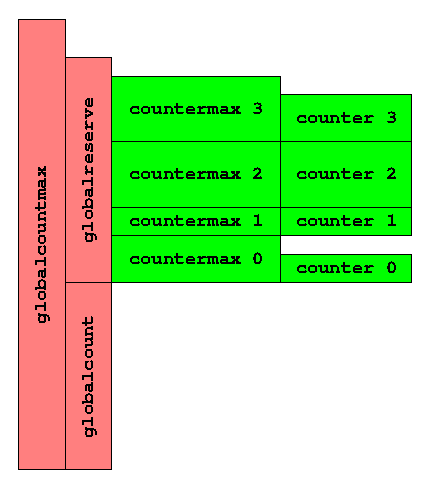
\includegraphics{count/count_lim}}
\end{center}
\caption{Simple Limit Counter Variable Relationships}
\label{fig:count:Simple Limit Counter Variable Relationships}
\end{figure}

Figure~\ref{fig:count:Simple Limit Counter Variables}
shows both the per-thread and global variables used by this
implementation.
The per-thread \co{counter} and \co{countermax} variables are the
corresponding thread's local counter and the upper bound on that
counter, respectively.
The \co{globalcountmax} variable on line~3 contains the upper
bound for the aggregate counter, and the \co{globalcount} variable
on line~4 is the global counter.
The sum of \co{globalcount} and each thread's \co{counter} gives
the aggregate value of the overall counter.
The \co{globalreserve} variable on line~5 is the sum of all of the
per-thread \co{countermax} variables.
The relationship among these variables is shown by
Figure~\ref{fig:count:Simple Limit Counter Variable Relationships}:
\begin{enumerate}
\item	The sum of \co{globalcount} and \co{globalreserve} must
	be less than or equal to \co{globalcountmax}.
\item	The sum of all threads' \co{countermax} values must be
	less than or equal to \co{globalreserve}.
\item	Each thread's \co{counter} must be less than or equal to
	that thread's \co{countermax}.
\end{enumerate}

Each element of the \co{counterp[]} array references the corresponding
thread's \co{counter} variable, and, finally, the \co{gblcnt_mutex}
spinlock guards all of the global variables, in other words, no thread
is permitted to access or modify any of the global variables unless it
has acquired \co{gblcnt_mutex}.

\begin{figure}[tbp]
{ \scriptsize
\begin{verbatim}
  1 int add_count(unsigned long delta)
  2 {
  3   if (countermax - counter >= delta) {
  4     counter += delta;
  5     return 1;
  6   }
  7   spin_lock(&gblcnt_mutex);
  8   globalize_count();
  9   if (globalcountmax -
 10       globalcount - globalreserve < delta) {
 11     spin_unlock(&gblcnt_mutex);
 12     return 0;
 13   }
 14   globalcount += delta;
 15   balance_count();
 16   spin_unlock(&gblcnt_mutex);
 17   return 1;
 18 }
 19 
 20 int sub_count(unsigned long delta)
 21 {
 22   if (counter >= delta) {
 23     counter -= delta;
 24     return 1;
 25   }
 26   spin_lock(&gblcnt_mutex);
 27   globalize_count();
 28   if (globalcount < delta) {
 29     spin_unlock(&gblcnt_mutex);
 30     return 0;
 31   }
 32   globalcount -= delta;
 33   balance_count();
 34   spin_unlock(&gblcnt_mutex);
 35   return 1;
 36 }
 37 
 38 unsigned long read_count(void)
 39 {
 40   int t;
 41   unsigned long sum;
 42 
 43   spin_lock(&gblcnt_mutex);
 44   sum = globalcount;
 45   for_each_thread(t)
 46     if (counterp[t] != NULL)
 47       sum += *counterp[t];
 48   spin_unlock(&gblcnt_mutex);
 49   return sum;
 50 }
\end{verbatim}
}
\caption{Simple Limit Counter Add, Subtract, and Read}
\label{fig:count:Simple Limit Counter Add, Subtract, and Read}
\end{figure}

Figure~\ref{fig:count:Simple Limit Counter Add, Subtract, and Read}
shows the \co{add_count()}, \co{sub_count()}, and \co{read_count()}
functions (\url{count_lim.c}).

Lines~1-18 show \co{add_count()}, which adds the specified value \co{delta}
to the counter.
Line~3 checks to see if there is room for \co{delta} on this thread's
\co{counter}, and, if so, line~4 adds it and line~6 returns success.
This is the \co{add_counter()} fastpath, and it does no atomic operations,
references only per-thread variables, and should not incur any cache misses.

\QuickQuiz{}
	What is with the strange form of the condition on line~3 of
	Figure~\ref{fig:count:Simple Limit Counter Add, Subtract, and Read}?
	Why not the following more intuitive form of the fastpath?

	\vspace{5pt}
	\begin{minipage}[t]{\columnwidth}
	\small
	\begin{verbatim}
  3 if (counter + delta <= countermax){
  4   counter += delta;
  5   return 1;
  6 }
	\end{verbatim}
	\end{minipage}
	\vspace{5pt}
\QuickQuizAnswer{
	Two words.
	``Integer overflow.''

	Try the above formulation with \co{counter} equal to 10 and
	\co{delta} equal to \co{ULONG_MAX}.
	Then try it again with the code shown in
	Figure~\ref{fig:count:Simple Limit Counter Add, Subtract, and Read}.

	A good understanding of integer overflow will be required for
	the rest of this example, so if you have never dealt with
	integer overflow before, please try several examples to get
	the hang of it.
	Integer overflow can sometimes be more difficult to get right
	than parallel algorithms!
} \QuickQuizEnd

If the test on line~3 fails, we must access global variables, and thus
must acquire \co{gblcnt_mutex} on line~7, which we release on line~11
in the failure case or on line~16 in the success case.
Line~8 invokes \co{globalize_count()}, shown in
Figure~\ref{fig:count:Simple Limit Counter Utility Functions},
which clears the thread-local variables, adjusting the global variables
as needed, thus simplifying global processing.
(But don't take \emph{my} word for it, try coding it yourself!)
Lines~9 and 10 check to see if addition of \co{delta} can be accommodated,
with the meaning of the expression preceding the less-than sign shown in
Figure~\ref{fig:count:Simple Limit Counter Variable Relationships}
as the difference in height of the two red bars.
If the addition of \co{delta} cannot be accommodated, then
line~11 (as noted earlier) releases \co{gblcnt_mutex} and line~12
returns indicating failure.

Otherwise, line~14 adds \co{delta} to \co{globalcount},
line~15 invokes \co{balance_count()} (shown in
Figure~\ref{fig:count:Simple Limit Counter Utility Functions})
in order to update both the global and the per-thread variables
(hopefully setting this thread's \co{countermax} to re-enable the
fastpath),
if appropriate, to re-enable fastpath processing, line~16 release
\co{gblcnt_mutex} (again, as noted earlier), and, finally,
line~17 returns indicating success.

\QuickQuiz{}
	Why does \co{globalize_count()} zero the per-thread variables,
	only to later call \co{balance_count()} to refill them in
	Figure~\ref{fig:count:Simple Limit Counter Add, Subtract, and Read}?
	Why not just leave the per-thread variables non-zero?
\QuickQuizAnswer{
	That is in fact what an earlier version of this code did.
	But addition and subtraction are extremely cheap, and handling
	all of the special cases that arise is quite complex.
	Again, feel free to try it yourself, but beware of integer
	overflow!
} \QuickQuizEnd

Lines~20-36 show \co{sub_count()}, which subtracts the specified
\co{delta} from the counter.
Line~22 checks to see if the per-thread counter can accommodate
this subtraction, and, if so, line~23 does the subtraction and
line~24 returns success.
These lines form \co{sub_count()}'s fastpath, and, as with
\co{add_count()}, this fastpath executes no costly operations.

If the fastpath cannot accommodate subtraction of \co{delta},
execution proceeds to the slowpath on lines~26-35.
Because the slowpath must access global state, line~26
acquires \co{gblcnt_mutex}, which is release either by line~29
(in case of failure) or by line~34 (in case of success).
Line~27 invokes \co{globalize_count()}, shown in
Figure~\ref{fig:count:Simple Limit Counter Utility Functions},
which again clears the thread-local variables, adjusting the global variables
as needed.
Line~28 checks to see if the counter can accommodate subtracting
\co{delta}, and, if not, line~29 releases \co{gblcnt_mutex}
(as noted earlier) and line~30 returns failure.

\QuickQuiz{}
	Given that \co{globalreserve} counted against us in \co{add_count()},
	why doesn't it count for us in \co{sub_count()} in
	Figure~\ref{fig:count:Simple Limit Counter Add, Subtract, and Read}?
\QuickQuizAnswer{
	The \co{globalreserve} variable tracks the sum of all threads'
	\co{countermax} variables.
	The sum of these threads' \co{counter} variables might be anywhere
	from zero to \co{globalreserve}.
	We must therefore take a conservative approach, assuming that
	all threads' \co{counter} variables are full in \co{add_count()}
	and that they are all empty in \co{sub_count()}.

	But remember this question, as we will come back to it later.
} \QuickQuizEnd

If, on the other hand, line~28 finds that the counter \emph{can}
accommodate subtracting \co{delta}, then line~32 does the subtraction,
line~33 invokes \co{balance_count()} (shown in
Figure~\ref{fig:count:Simple Limit Counter Utility Functions})
in order to update both global and per-thread variables
(hopefully re-enabling the fastpath),
line~34 releases \co{gblcnt_mutex}, and line~35 returns success.

\QuickQuiz{}
	Why have both \co{add_count()} and \co{sub_count()} in
	Figure~\ref{fig:count:Simple Limit Counter Add, Subtract, and Read}?
	Why not simply pass a negative number to \co{add_count()}?
\QuickQuizAnswer{
	Given that \co{add_count()} takes an \co{unsigned} \co{long}
	as its argument, it is going to be a bit tough to pass it a
	negative number.
	And unless you have some anti-matter memory, there is little
	point in allowing negative numbers when counting the number
	of structures in use!
} \QuickQuizEnd

Lines~38-50 show \co{read_count()}, which returns the aggregate value
of the counter.
It acquires \co{gblcnt_mutex} on line~43 and releases it on line 48,
excluding global operations from \co{add_count()} and \co{sub_count()},
and, as we will see, also excluding thread creation and exit.
Line~44 initializes local variable \co{sum} to the value of
\co{globalcount}, and then the loop spanning lines~45-47 sums the
per-thread \co{counter} variables.
Line~49 then returns the sum.

\begin{figure}[tbp]
{ \scriptsize
\begin{verbatim}
  1 static void globalize_count(void)
  2 {
  3   globalcount += counter;
  4   counter = 0;
  5   globalreserve -= countermax;
  6   countermax = 0;
  7 }
  8 
  9 static void balance_count(void)
 10 {
 11   countermax = globalcountmax -
 12                globalcount - globalreserve;
 13   countermax /= num_online_threads();
 14   globalreserve += countermax;
 15   counter = countermax / 2;
 16   if (counter > globalcount)
 17     counter = globalcount;
 18   globalcount -= counter;
 19 }
 20 
 21 void count_register_thread(void)
 22 {
 23   int idx = smp_thread_id();
 24 
 25   spin_lock(&gblcnt_mutex);
 26   counterp[idx] = &counter;
 27   spin_unlock(&gblcnt_mutex);
 28 }
 29 
 30 void count_unregister_thread(int nthreadsexpected)
 31 {
 32   int idx = smp_thread_id();
 33 
 34   spin_lock(&gblcnt_mutex);
 35   globalize_count();
 36   counterp[idx] = NULL;
 37   spin_unlock(&gblcnt_mutex);
 38 }
\end{verbatim}
}
\caption{Simple Limit Counter Utility Functions}
\label{fig:count:Simple Limit Counter Utility Functions}
\end{figure}

Figure~\ref{fig:count:Simple Limit Counter Utility Functions}
shows a number of utility functions that support the \co{add_count()}
\co{sub_count()}, and \co{read_count()} primitives shown in
Figure~\ref{fig:count:Simple Limit Counter Add, Subtract, and Read}.

Lines~1-7 show \co{globalize_count()}, which zeros the current thread's
per-thread counters, adjusting the global variables appropriately.
It is important to note that this function does not change the aggregate
value of the counter, but instead changes how the counter's current value
is represented.
Line~3 adds the thread's \co{counter} variable to \co{globalcount},
and line~4 zeroes \co{counter}.
Similarly, line~5 subtracts the per-thread \co{countermax} from
\co{globalreserve}, and line~6 zeroes \co{countermax}.
It is helpful to refer to
Figure~\ref{fig:count:Simple Limit Counter Variable Relationships}
when reading both this function and \co{balance_count()}, which is next.

Lines~9-19 show \co{balance_count()}, which is, roughly speaking
the inverse of \co{globalize_count()}.
This function sets the current thread's \co{counter} and \co{countermax}
variables (with corresponding adjustments to \co{globalcount}
and \co{globalreserve}) in an attempt to promote use of
\co{add_count()}'s and \co{sub_count()}'s fastpaths.
As with \co{globalize_count()}, \co{balance_count()} does not change
the aggregate value of the counter.
Lines~11-13 compute this thread's share of that portion of
\co{globalcountmax} that is not already covered by either
\co{globalcount} or \co{globalreserve}, and assign the
computed quantity to this thread's \co{countermax}.
Line~14 makes the corresponding adjustment to \co{globalreserve}.
Line~15 sets this thread's \co{counter} to the middle of the range
from zero to \co{countermax}.
Line~16 checks to see whether \co{globalcount} can in fact accommodate
this value of \co{counter}, and, if not, line~17 decreases \co{counter}
accordingly.
Finally, in either case, line~18 makes the corresponding adjustment to
\co{globalcount}.

\QuickQuiz{}
	Why set \co{counter} to \co{countermax / 2} in line~15 of
	Figure~\ref{fig:count:Simple Limit Counter Utility Functions}?
	Wouldn't it be simpler to just take \co{countermax} counts?
\QuickQuizAnswer{
	First, it really is reserving \co{countermax} counts
	(see line~14), however,
	it adjusts so that only half of these are actually in use
	by the thread at the moment.
	This allows the thread to carry out at least \co{countermax / 2}
	increments or decrements before having to refer back to
	\co{globalcount} again.

	Note that the accounting in \co{globalcount} remains accurate,
	thanks to the adjustment in line~18.
} \QuickQuizEnd

Lines~21-28 show \co{count_register_thread()}, which sets up state for
newly created threads.
This function simply installs
a pointer to the newly created thread's \co{counter} variable into
the corresponding entry of the \co{counterp[]} array under the protection
of \co{gblcnt_mutex}.

Finally, lines~30-38 show \co{count_unregister_thread()}, which tears down
state for a soon-to-be-exiting thread.
Line~34 acquires \co{gblcnt_mutex} and line~37 releases it.
Line~35 invokes \co{globalize_count()} to clear out this thread's
counter state, and line~36 clears this thread's entry in the
\co{counterp[]} array.

\subsection{Simple Limit Counter Discussion}

This type of counter is quite fast when aggregate values are near zero,
with some overhead due to the comparison and branch in both
\co{add_count()}'s and \co{sub_count()}'s fastpaths.
However, the use of a per-thread \co{countermax} reserve means that
\co{add_count()} can fail even when
the aggregate value of the counter is nowhere near \co{globalcountmax}.
Similarly, \co{sub_count()} can fail
even when the aggregate value of the counter is nowhere near zero.

In many cases, this is unacceptable.
Even if the \co{globalcountmax} is intended to be an approximate limit,
there is usually a limit to exactly how much approximation can be tolerated.
One way to limit the degree of approximation is to impose an upper limit
on the value of the per-thread \co{countermax} instances.
This task is undertaken in the next section.

\subsection{Approximate Limit Counter Implementation}
\label{sec:count:Approximate Limit Counter Implementation}

\begin{figure}[tbp]
{ \scriptsize
\begin{verbatim}
  1 unsigned long __thread counter = 0;
  2 unsigned long __thread countermax = 0;
  3 unsigned long globalcountmax = 10000;
  4 unsigned long globalcount = 0;
  5 unsigned long globalreserve = 0;
  6 unsigned long *counterp[NR_THREADS] = { NULL };
  7 DEFINE_SPINLOCK(gblcnt_mutex);
  8 #define MAX_COUNTERMAX 100
\end{verbatim}
}
\caption{Approximate Limit Counter Variables}
\label{fig:count:Approximate Limit Counter Variables}
\end{figure}

\begin{figure}[tbp]
{ \scriptsize
\begin{verbatim}
  1 static void balance_count(void)
  2 {
  3   countermax = globalcountmax -
  4                globalcount - globalreserve;
  5   countermax /= num_online_threads();
  6   if (countermax > MAX_COUNTERMAX)
  7     countermax = MAX_COUNTERMAX;
  8   globalreserve += countermax;
  9   counter = countermax / 2;
 10   if (counter > globalcount)
 11     counter = globalcount;
 12   globalcount -= counter;
 13 }
\end{verbatim}
}
\caption{Approximate Limit Counter Balancing}
\label{fig:count:Approximate Limit Counter Balancing}
\end{figure}

Because this implementation (\url{count_lim_app.c}) is quite similar to
that in the previous section
(Figures~\ref{fig:count:Simple Limit Counter Variables},
\ref{fig:count:Simple Limit Counter Add, Subtract, and Read}, and
\ref{fig:count:Simple Limit Counter Utility Functions}),
only the changes are shown here.
Figure~\ref{fig:count:Approximate Limit Counter Variables}
is identical to
Figure~\ref{fig:count:Simple Limit Counter Variables},
with the addition of \co{MAX_COUNTERMAX}, which sets the maximum
permissible value of the per-thread \co{countermax} variable.

Similarly,
Figure~\ref{fig:count:Approximate Limit Counter Balancing}
is identical to the \co{balance_count()} function in
Figure~\ref{fig:count:Simple Limit Counter Utility Functions}),
with the addition of lines~6 and 7, which enforce the
\co{MAX_COUNTERMAX} limit on the per-thread \co{countermax} variable.

\subsection{Approximate Limit Counter Discussion}

These changes greatly reduce the limit inaccuracy seen in the previous version,
but present another problem: any given value of \co{MAX_COUNTERMAX}
will cause a workload-dependent fraction of accesses to fall off the
fastpath.
As the number of threads increase, non-fastpath execution will become both
a performance and a scalability problem.
However, we will defer this problem and turn instead to counters
with exact limits.

\section{Exact Limit Counters}
\label{sec:count:Exact Limit Counters}

To solve the exact structure-allocation limit problem noted in the
Quick Quiz on
page~\pageref{chp:Counting},
we need a limit counter that can tell exactly when its limits are
exceeded.
One way of implementing such a limit counter is to
cause threads that have reserved counts to give them up.
One way to do this is to use atomic instructions.
Of course, atomic instructions will slow down the fastpath, but on the
other hand, it would be silly not to at least give them a try.

\subsection{Atomic Limit Counter Implementation}
\label{sec:count:Atomic Limit Counter Implementation}

Unfortunately, when causing a given thread to give up its count, it is
necessary to atomically manipulate both that thread's \co{counter}
and \co{countermax} variables.
The usual way to do this is to combine these two variables into a
single variable,
for example, given a 32-bit variable, using the high-order 16 bits to
represent \co{counter} and the low-order 16 bits to represent
\co{countermax}.

\begin{figure}[tbp]
{ \scriptsize
\begin{verbatim}
  1 atomic_t __thread ctrandmax = ATOMIC_INIT(0);
  2 unsigned long globalcountmax = 10000;
  3 unsigned long globalcount = 0;
  4 unsigned long globalreserve = 0;
  5 atomic_t *counterp[NR_THREADS] = { NULL };
  6 DEFINE_SPINLOCK(gblcnt_mutex);
  7 #define CM_BITS (sizeof(atomic_t) * 4)
  8 #define MAX_COUNTERMAX ((1 << CM_BITS) - 1)
  9 
 10 static void
 11 split_ctrandmax_int(int cami, int *c, int *cm)
 12 {
 13   *c = (cami >> CM_BITS) & MAX_COUNTERMAX;
 14   *cm = cami & MAX_COUNTERMAX;
 15 }
 16 
 17 static void
 18 split_ctrandmax(atomic_t *cam, int *old,
 19                     int *c, int *cm)
 20 {
 21   unsigned int cami = atomic_read(cam);
 22 
 23   *old = cami;
 24   split_ctrandmax_int(cami, c, cm);
 25 }
 26 
 27 static int merge_ctrandmax(int c, int cm)
 28 {
 29   unsigned int cami;
 30 
 31   cami = (c << CM_BITS) | cm;
 32   return ((int)cami);
 33 }
\end{verbatim}
}
\caption{Atomic Limit Counter Variables and Access Functions}
\label{fig:count:Atomic Limit Counter Variables and Access Functions}
\end{figure}

The variables and access functions for a simple atomic limit counter
are shown in
Figure~\ref{fig:count:Atomic Limit Counter Variables and Access Functions}
(\url{count_lim_atomic.c}).
The \co{counter} and \co{countermax} variables in earlier algorithms
are combined into the single variable \co{ctrandmax} shown on
line~1, with \co{counter} in the upper half and \co{countermax} in
the lower half.
This variable is of type \co{atomic_t}, which has an underlying
representation of \co{int}.

Lines~2-6 show the definitions for \co{globalcountmax}, \co{globalcount},
\co{globalreserve}, \co{counterp}, and \co{gblcnt_mutex}, all of which
take on roles similar to their counterparts in
Figure~\ref{fig:count:Approximate Limit Counter Variables}.
Line~7 defines \co{CM_BITS}, which gives the number of bits in each half
of \co{ctrandmax}, and line~8 defines \co{MAX_COUNTERMAX}, which
gives the maximum value that may be held in either half of
\co{ctrandmax}.

\QuickQuiz{}
	In what way does line~7 of
	Figure~\ref{fig:count:Atomic Limit Counter Variables and Access Functions}
	violate the C standard?
\QuickQuizAnswer{
	It assumes eight bits per byte.
	This assumption does hold for all current commodity microprocessors
	that can be easily assembled into shared-memory multiprocessors,
	but certainly does not hold for all computer systems that have
	ever run C code.
	(What could you do instead in order to comply with the C
	standard?  What drawbacks would it have?)
} \QuickQuizEnd

Lines~10-15 show the \co{split_ctrandmax_int()} function, which,
when given the underlying \co{int} from the \co{atomic_t
ctrandmax} variable.
Line~13 isolates the most-significant half of this \co{int},
placing the result as specified by argument \co{c},
and line~14 isolates the least-significant half of this \co{int},
placing the result as specified by argument \co{cm}.

Lines~17-25 show the \co{split_ctrandmax()} function, which
picks up the underlying \co{int} from the specified variable
on line~21, stores it as specified by the \co{old} argument on
line~23, and then invokes \co{split_ctrandmax_int()} to split
it on line~24.

\QuickQuiz{}
	Given that there is only one \co{ctrandmax} variable,
	why bother passing in a pointer to it on line~18 of
	Figure~\ref{fig:count:Atomic Limit Counter Variables and Access Functions}?
\QuickQuizAnswer{
	There is only one \co{ctrandmax} variable \emph{per thread}.
	Later, we will see code that needs to pass other threads'
	\co{ctrandmax} variables to \co{split_ctrandmax()}.
} \QuickQuizEnd

Lines~27-33 show the \co{merge_ctrandmax()} function, which
can be thought of as the inverse of \co{split_ctrandmax()}.
Line~31 merges the \co{counter} and \co{countermax}
values passed in \co{c} and \co{cm}, respectively, and returns
the result.

\QuickQuiz{}
	Why does \co{merge_ctrandmax()} in
	Figure~\ref{fig:count:Atomic Limit Counter Variables and Access Functions}
	return an \co{int} rather than storing directly into an
	\co{atomic_t}?
\QuickQuizAnswer{
	Later, we will see that we need the \co{int} return to pass
	to the \co{atomic_cmpxchg()} primitive.
} \QuickQuizEnd

\begin{figure}[tbp]
{ \scriptsize
\begin{verbatim}
  1 int add_count(unsigned long delta)
  2 {
  3   int c;
  4   int cm;
  5   int old;
  6   int new;
  7 
  8   do {
  9     split_ctrandmax(&ctrandmax, &old, &c, &cm);
 10     if (delta > MAX_COUNTERMAX || c + delta > cm)
 11       goto slowpath;
 12     new = merge_ctrandmax(c + delta, cm);
 13   } while (atomic_cmpxchg(&ctrandmax,
 14                           old, new) != old);
 15   return 1;
 16 slowpath:
 17   spin_lock(&gblcnt_mutex);
 18   globalize_count();
 19   if (globalcountmax - globalcount -
 20       globalreserve < delta) {
 21     flush_local_count();
 22     if (globalcountmax - globalcount -
 23         globalreserve < delta) {
 24       spin_unlock(&gblcnt_mutex);
 25       return 0;
 26     }
 27   }
 28   globalcount += delta;
 29   balance_count();
 30   spin_unlock(&gblcnt_mutex);
 31   return 1;
 32 }
 33 
 34 int sub_count(unsigned long delta)
 35 {
 36   int c;
 37   int cm;
 38   int old;
 39   int new;
 40 
 41   do {
 42     split_ctrandmax(&ctrandmax, &old, &c, &cm);
 43     if (delta > c)
 44       goto slowpath;
 45     new = merge_ctrandmax(c - delta, cm);
 46   } while (atomic_cmpxchg(&ctrandmax,
 47                           old, new) != old);
 48   return 1;
 49 slowpath:
 50   spin_lock(&gblcnt_mutex);
 51   globalize_count();
 52   if (globalcount < delta) {
 53     flush_local_count();
 54     if (globalcount < delta) {
 55       spin_unlock(&gblcnt_mutex);
 56       return 0;
 57     }
 58   }
 59   globalcount -= delta;
 60   balance_count();
 61   spin_unlock(&gblcnt_mutex);
 62   return 1;
 63 }
\end{verbatim}
}
\caption{Atomic Limit Counter Add and Subtract}
\label{fig:count:Atomic Limit Counter Add and Subtract}
\end{figure}

Figure~\ref{fig:count:Atomic Limit Counter Add and Subtract}
shows the \co{add_count()}, \co{sub_count()}, and
\co{read_count()} functions.

Lines~1-32 show \co{add_count()}, whose fastpath spans lines~8-15,
with the remainder of the function being the slowpath.
Lines~8-14 of the fastpath form a compare-and-swap (CAS) loop, with
the \co{atomic_cmpxchg()} primitives on lines~13-14 performing the
actual CAS.
Line~9 splits the current thread's \co{ctrandmax} variable into its
\co{counter} (in \co{c}) and \co{countermax} (in \co{cm}) components,
while placing the underlying \co{int} into \co{old}.
Line~10 checks whether the amount \co{delta} can be accommodated
locally (taking care to avoid integer overflow), and if not,
line~11 transfers to the slowpath.
Otherwise, line~11 combines an updated \co{counter} value with the
original \co{countermax} value into \co{new}.
The \co{atomic_cmpxchg()} primitive on lines~13-14 then atomically
compares this thread's \co{ctrandmax} variable to \co{old},
updating its value to \co{new} if the comparison succeeds.
If the comparison succeeds, line~15 returns success, otherwise,
execution continues in the loop at line~9.

\QuickQuiz{}
	Yecch!
	Why the ugly \co{goto} on line~11 of
	Figure~\ref{fig:count:Atomic Limit Counter Add and Subtract}?
	Haven't you heard of the \co{break} statement???
\QuickQuizAnswer{
	Replacing the \co{goto} with a \co{break} would require keeping
	a flag to determine whether or not line~15 should return, which
	is not the sort of thing you want on a fastpath.
	If you really hate the \co{goto} that much, your best bet would
	be to pull the fastpath into a separate function that returned
	success or failure, with ``failure'' indicating a need for the
	slowpath.
	This is left as an exercise for goto-hating readers.
} \QuickQuizEnd

\QuickQuiz{}
	Why would the \co{atomic_cmpxchg()} primitive at lines~13-14 of
	Figure~\ref{fig:count:Atomic Limit Counter Add and Subtract}
	ever fail?
	After all, we picked up its old value on line~9 and have not
	changed it!
\QuickQuizAnswer{
	Later, we will see how the \co{flush_local_count()} function in
	Figure~\ref{fig:count:Atomic Limit Counter Utility Functions 1}
	might update this thread's \co{ctrandmax} variable concurrently
	with the execution of the fastpath on lines~8-14 of
	Figure~\ref{fig:count:Atomic Limit Counter Add and Subtract}.
} \QuickQuizEnd

Lines~16-32 of
Figure~\ref{fig:count:Atomic Limit Counter Add and Subtract}
show \co{add_count()}'s slowpath, which is protected by \co{gblcnt_mutex},
which is acquired on line~17 and released on lines~24 and 30.
Line~18 invokes \co{globalize_count()}, which moves this thread's
state to the global counters.
Lines~19-20 check whether the \co{delta} value can be accommodated by
the current global state, and, if not, line~21 invokes
\co{flush_local_count()} to flush all threads' local state to the
global counters, and then lines~22-23 recheck whether \co{delta} can
be accommodated.
If, after all that, the addition of \co{delta} still cannot be accommodated,
then line~24 releases \co{gblcnt_mutex} (as noted earlier), and
then line~25 returns failure.

Otherwise, line~28 adds \co{delta} to the global counter, line~29
spreads counts to the local state if appropriate, line~30 releases
\co{gblcnt_mutex} (again, as noted earlier), and finally, line 31
returns success.

Lines~34-63 of
Figure~\ref{fig:count:Atomic Limit Counter Add and Subtract}
show \co{sub_count()}, which is structured similarly to
\co{add_count()}, having a fastpath on lines~41-48 and a slowpath on
lines~49-62.
A line-by-line analysis of this function is left as an exercise to
the reader.

\begin{figure}[tbp]
{ \scriptsize
\begin{verbatim}
  1 unsigned long read_count(void)
  2 {
  3   int c;
  4   int cm;
  5   int old;
  6   int t;
  7   unsigned long sum;
  8 
  9   spin_lock(&gblcnt_mutex);
 10   sum = globalcount;
 11   for_each_thread(t)
 12     if (counterp[t] != NULL) {
 13       split_ctrandmax(counterp[t], &old, &c, &cm);
 14       sum += c;
 15     }
 16   spin_unlock(&gblcnt_mutex);
 17   return sum;
 18 }
\end{verbatim}
}
\caption{Atomic Limit Counter Read}
\label{fig:count:Atomic Limit Counter Read}
\end{figure}

Figure~\ref{fig:count:Atomic Limit Counter Read} shows \co{read_count()}.
Line~9 acquires \co{gblcnt_mutex} and line~16 releases it.
Line~10 initializes local variable \co{sum} to the value of
\co{globalcount}, and the loop spanning lines~11-15 adds the
per-thread counters to this sum, isolating each per-thread counter
using \co{split_ctrandmax} on line 13.
Finally, line~17 returns the sum.

\begin{figure}[tbp]
{ \scriptsize
\begin{verbatim}
  1 static void globalize_count(void)
  2 {
  3   int c;
  4   int cm;
  5   int old;
  6 
  7   split_ctrandmax(&ctrandmax, &old, &c, &cm);
  8   globalcount += c;
  9   globalreserve -= cm;
 10   old = merge_ctrandmax(0, 0);
 11   atomic_set(&ctrandmax, old);
 12 }
 13 
 14 static void flush_local_count(void)
 15 {
 16   int c;
 17   int cm;
 18   int old;
 19   int t;
 20   int zero;
 21 
 22   if (globalreserve == 0)
 23     return;
 24   zero = merge_ctrandmax(0, 0);
 25   for_each_thread(t)
 26     if (counterp[t] != NULL) {
 27       old = atomic_xchg(counterp[t], zero);
 28       split_ctrandmax_int(old, &c, &cm);
 29       globalcount += c;
 30       globalreserve -= cm;
 31     }
 32 }
\end{verbatim}
}
\caption{Atomic Limit Counter Utility Functions 1}
\label{fig:count:Atomic Limit Counter Utility Functions 1}
\end{figure}

\begin{figure}[tbp]
{ \scriptsize
\begin{verbatim}
  1 static void balance_count(void)
  2 {
  3   int c;
  4   int cm;
  5   int old;
  6   unsigned long limit;
  7 
  8   limit = globalcountmax - globalcount -
  9           globalreserve;
 10   limit /= num_online_threads();
 11   if (limit > MAX_COUNTERMAX)
 12     cm = MAX_COUNTERMAX;
 13   else
 14     cm = limit;
 15   globalreserve += cm;
 16   c = cm / 2;
 17   if (c > globalcount)
 18     c = globalcount;
 19   globalcount -= c;
 20   old = merge_ctrandmax(c, cm);
 21   atomic_set(&ctrandmax, old);
 22 }
 23 
 24 void count_register_thread(void)
 25 {
 26   int idx = smp_thread_id();
 27 
 28   spin_lock(&gblcnt_mutex);
 29   counterp[idx] = &ctrandmax;
 30   spin_unlock(&gblcnt_mutex);
 31 }
 32 
 33 void count_unregister_thread(int nthreadsexpected)
 34 {
 35   int idx = smp_thread_id();
 36 
 37   spin_lock(&gblcnt_mutex);
 38   globalize_count();
 39   counterp[idx] = NULL;
 40   spin_unlock(&gblcnt_mutex);
 41 }
\end{verbatim}
}
\caption{Atomic Limit Counter Utility Functions 2}
\label{fig:count:Atomic Limit Counter Utility Functions 2}
\end{figure}

Figures~\ref{fig:count:Atomic Limit Counter Utility Functions 1}
and~\ref{fig:count:Atomic Limit Counter Utility Functions 2}
shows the utility functions
\co{globalize_count()},
\co{flush_local_count()},
\co{balance_count()},
\co{count_register_thread()}, and
\co{count_unregister_thread()}.
The code for \co{globalize_count()} is shown on lines~1-12,
of Figure~\ref{fig:count:Atomic Limit Counter Utility Functions 1} and
is similar to that of previous algorithms, with the addition of
line~7, which is now required to split out \co{counter} and
\co{countermax} from \co{ctrandmax}.

The code for \co{flush_local_count()}, which moves all threads' local
counter state to the global counter, is shown on lines~14-32.
Line~22 checks to see if the value of \co{globalreserve} permits
any per-thread counts, and, if not, line~23 returns.
Otherwise, line~24 initializes local variable \co{zero} to a combined
zeroed \co{counter} and \co{countermax}.
The loop spanning lines~25-31 sequences through each thread.
Line~26 checks to see if the current thread has counter state,
and, if so, lines~27-30 move that state to the global counters.
Line~27 atomically fetches the current thread's state
while replacing it with zero.
Line~28 splits this state into its \co{counter} (in local variable \co{c})
and \co{countermax} (in local variable \co{cm}) components.
Line~29 adds this thread's \co{counter} to \co{globalcount}, while
line~30 subtracts this thread's \co{countermax} from \co{globalreserve}.

\QuickQuiz{}
	What stops a thread from simply refilling its
	\co{ctrandmax} variable immediately after
	\co{flush_local_count()} on line 14 of
	Figure~\ref{fig:count:Atomic Limit Counter Utility Functions 1}
	empties it?
\QuickQuizAnswer{
	This other thread cannot refill its \co{ctrandmax}
	until the caller of \co{flush_local_count()} releases the
	\co{gblcnt_mutex}.
	By that time, the caller of \co{flush_local_count()} will have
	finished making use of the counts, so there will be no problem
	with this other thread refilling --- assuming that the value
	of \co{globalcount} is large enough to permit a refill.
} \QuickQuizEnd

\QuickQuiz{}
	What prevents concurrent execution of the fastpath of either
	\co{atomic_add()} or \co{atomic_sub()} from interfering with
	the \co{ctrandmax} variable while
	\co{flush_local_count()} is accessing it on line 27 of
	Figure~\ref{fig:count:Atomic Limit Counter Utility Functions 1}
	empties it?
\QuickQuizAnswer{
	Nothing.
	Consider the following three cases:
	\begin{enumerate}
	\item	If \co{flush_local_count()}'s \co{atomic_xchg()} executes
		before the \co{split_ctrandmax()} of either fastpath,
		then the fastpath will see a zero \co{counter} and
		\co{countermax}, and will thus transfer to the slowpath
		(unless of course \co{delta} is zero).
	\item	If \co{flush_local_count()}'s \co{atomic_xchg()} executes
		after the \co{split_ctrandmax()} of either fastpath,
		but before that fastpath's \co{atomic_cmpxchg()},
		then the \co{atomic_cmpxchg()} will fail, causing the
		fastpath to restart, which reduces to case~1 above.
	\item	If \co{flush_local_count()}'s \co{atomic_xchg()} executes
		after the \co{atomic_cmpxchg()} of either fastpath,
		then the fastpath will (most likely) complete successfully
		before \co{flush_local_count()} zeroes the thread's
		\co{ctrandmax} variable.
	\end{enumerate}
	Either way, the race is resolved correctly.
} \QuickQuizEnd

Lines~1-22 on
Figure~\ref{fig:count:Atomic Limit Counter Utility Functions 2}
show the code for \co{balance_count()}, which refills
the calling thread's local \co{ctrandmax} variable.
This function is quite similar to that of the preceding algorithms,
with changes required to handle the merged \co{ctrandmax} variable.
Detailed analysis of the code is left as an exercise for the reader,
as it is with the \co{count_register_thread()} function starting on
line~24 and the \co{count_unregister_thread()} function starting on
line~33.

\QuickQuiz{}
	Given that the \co{atomic_set()} primitive does a simple
	store to the specified \co{atomic_t}, how can line~21 of
	\co{balance_count()} in
	Figure~\ref{fig:count:Atomic Limit Counter Utility Functions 2}
	work correctly in face of concurrent \co{flush_local_count()}
	updates to this variable?
\QuickQuizAnswer{
	The caller of both \co{balance_count()} and
	\co{flush_local_count()} hold \co{gblcnt_mutex}, so
	only one may be executing at a given time.
} \QuickQuizEnd

\subsection{Atomic Limit Counter Discussion}

This is the first implementation that actually allows the counter to
be run all the way to either of its limits, but it does so at the
expense of adding atomic operations to the fastpaths, which slow down
the fastpaths significantly.
Although some workloads might tolerate this slowdown, it is worthwhile
looking for algorithms with better read-side performance.
One such algorithm uses a signal handler to steal counts from other
threads.
Because signal handlers run in the context of the signaled thread,
atomic operations are not necessary, as shown in the next section.

\QuickQuiz{}
	But signal handlers can be migrated to some other
	CPU while running.
	Doesn't this possibility require that atomic instructions
	and memory barriers are required to reliably communicate
	between a thread and a signal handler that interrupts that
	thread?
\QuickQuizAnswer{
	No.
	If the signal handler is migrated to another CPU, then the
	interrupted thread is also migrated along with it.
} \QuickQuizEnd

\subsection{Signal-Theft Limit Counter Design}
\label{sec:count:Signal-Theft Limit Counter Design}

\begin{figure}[tb]
\begin{center}
\resizebox{2in}{!}{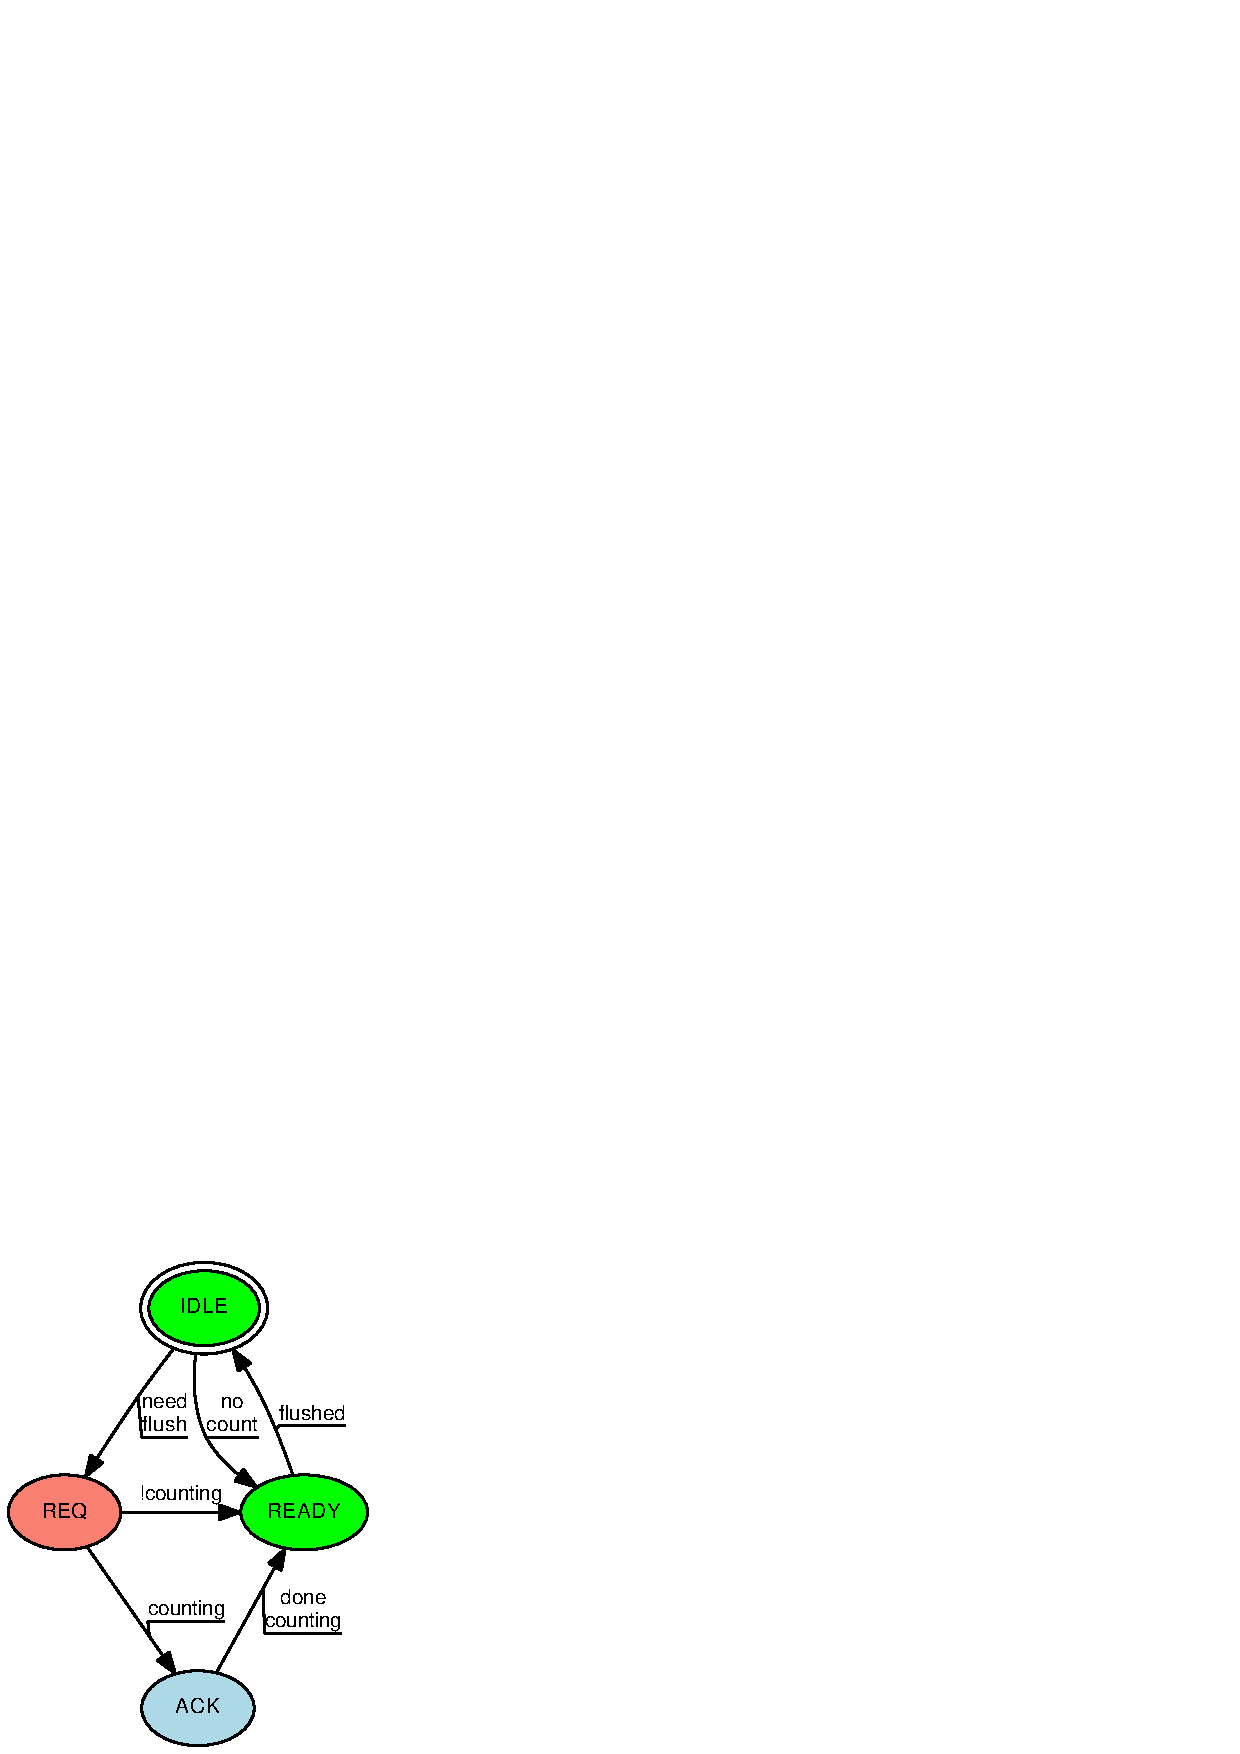
\includegraphics{count/sig-theft}}
\end{center}
\caption{Signal-Theft State Machine}
\label{fig:count:Signal-Theft State Machine}
\end{figure}

Figure~\ref{fig:count:Signal-Theft State Machine} shows the
state diagram.
The state machine starts out in the IDLE state, and when \co{add_count()}
or \co{sub_count()} find that the combination of the local thread's count
and the global count cannot accommodate the request, the corresponding
slowpath sets each thread's \co{theft} state to REQ (unless that thread
has no count, in which case it transitions directly to READY).
Only the slowpath, which holds the \co{gblcnt_mutex} lock, is permitted to
transition from the IDLE state, as indicated by the green color.
The slowpath then sends a signal to each thread, and the corresponding
signal handler checks the corresponding thread's \co{theft} and
\co{counting} variables.
If the \co{theft} state is not REQ, then the signal handler is not
permitted to change the state, and therefore simply returns.
Otherwise, if the \co{counting} variable is set, indicating that
the current thread's fastpath is in progress, the signal handler
sets the \co{theft} state to ACK, otherwise to READY.

If the \co{theft} state is ACK,
only the fastpath is permitted to change
the \co{theft} state, as indicated by the blue color.
When the fastpath completes, it sets the \co{theft} state to READY.

Once the slowpath sees a thread's \co{theft} state is READY, the
slowpath is permitted to steal that thread's count.
The slowpath then sets that thread's \co{theft} state to IDLE.

\QuickQuiz{}
	In Figure~\ref{fig:count:Signal-Theft State Machine}, why is
	the REQ \co{theft} state colored blue?
\QuickQuizAnswer{
	To indicate that only the fastpath is permitted to change the
	\co{theft} state.
} \QuickQuizEnd

\QuickQuiz{}
	In Figure~\ref{fig:count:Signal-Theft State Machine}, what is
	the point of having separate REQ and ACK \co{theft} states?
	Why not simplify the state machine by collapsing
	them into a single state?
	Then whichever of the signal handler or the fastpath gets there
	first could set the state to READY.
\QuickQuizAnswer{
	Reasons why collapsing the REQ and ACK states would be a very
	bad idea include:
	\begin{enumerate}
	\item	The slowpath uses the REQ and ACK states to determine
		whether the signal should be retransmitted.
		If the states were collapsed, the slowpath would have
		no choice but to send redundant signals, which would
		have the unhelpful effect of slowing down the fastpath.
	\item	The following race would result:
		\begin{enumerate}
		\item	The slowpath sets a given thread's state to REQACK.
		\item	That thread has just finished its fastpath, and
			notes the REQACK state.
		\item	The thread receives the signal, which also notes
			the REQACK state, and, because there is no fastpath
			in effect, sets the state to READY.
		\item	The slowpath notes the READY state, steals the
			count, and sets the state to IDLE, and completes.
		\item	The fastpath sets the state to READY, disabling
			further fastpath execution for this thread.
		\end{enumerate}
		The basic problem here is that the combined REQACK state
		can be referenced by both the signal handler and the
		fastpath.
		The clear separation maintained by the four-state
		setup ensures orderly state transitions.
	\end{enumerate}
	That said, you might well be able to make a three-state setup
	work correctly.
	If you do succeed, compare carefully to the four-state setup.
	Is the three-state solution really preferable, and why or why not?
} \QuickQuizEnd

\subsection{Signal-Theft Limit Counter Implementation}
\label{sec:count:Signal-Theft Limit Counter Implementation}

\begin{figure}[tbp]
{ \scriptsize
\begin{verbatim}
  1 #define THEFT_IDLE  0
  2 #define THEFT_REQ   1
  3 #define THEFT_ACK   2
  4 #define THEFT_READY 3
  5 
  6 int __thread theft = THEFT_IDLE;
  7 int __thread counting = 0;
  8 unsigned long __thread counter = 0;
  9 unsigned long __thread countermax = 0;
 10 unsigned long globalcountmax = 10000;
 11 unsigned long globalcount = 0;
 12 unsigned long globalreserve = 0;
 13 unsigned long *counterp[NR_THREADS] = { NULL };
 14 unsigned long *countermaxp[NR_THREADS] = { NULL };
 15 int *theftp[NR_THREADS] = { NULL };
 16 DEFINE_SPINLOCK(gblcnt_mutex);
 17 #define MAX_COUNTERMAX 100
\end{verbatim}
}
\caption{Signal-Theft Limit Counter Data}
\label{fig:count:Signal-Theft Limit Counter Data}
\end{figure}

Figure~\ref{fig:count:Signal-Theft Limit Counter Data}
(\url{count_lim_sig.c})
shows the data structures used by the signal-theft based counter
implementation.
Lines~1-7 define the states and values for the per-thread theft state machine
described in the preceding section.
Lines~8-17 are similar to earlier implementations, with the addition of
lines~14 and 15 to allow remote access to a thread's \co{countermax}
and \co{theft} variables, respectively.

\begin{figure}[tbp]
{ \scriptsize
\begin{verbatim}
  1 static void globalize_count(void)
  2 {
  3   globalcount += counter;
  4   counter = 0;
  5   globalreserve -= countermax;
  6   countermax = 0;
  7 }
  8 
  9 static void flush_local_count_sig(int unused)
 10 {
 11   if (ACCESS_ONCE(theft) != THEFT_REQ)
 12     return;
 13   smp_mb();
 14   ACCESS_ONCE(theft) = THEFT_ACK;
 15   if (!counting) {
 16     ACCESS_ONCE(theft) = THEFT_READY;
 17   }
 18   smp_mb();
 19 }
 20 
 21 static void flush_local_count(void)
 22 {
 23   int t;
 24   thread_id_t tid;
 25 
 26   for_each_tid(t, tid)
 27     if (theftp[t] != NULL) {
 28       if (*countermaxp[t] == 0) {
 29         ACCESS_ONCE(*theftp[t]) = THEFT_READY;
 30         continue;
 31       }
 32       ACCESS_ONCE(*theftp[t]) = THEFT_REQ;
 33       pthread_kill(tid, SIGUSR1);
 34     }
 35   for_each_tid(t, tid) {
 36     if (theftp[t] == NULL)
 37       continue;
 38     while (ACCESS_ONCE(*theftp[t]) != THEFT_READY) {
 39       poll(NULL, 0, 1);
 40       if (ACCESS_ONCE(*theftp[t]) == THEFT_REQ)
 41         pthread_kill(tid, SIGUSR1);
 42     }
 43     globalcount += *counterp[t];
 44     *counterp[t] = 0;
 45     globalreserve -= *countermaxp[t];
 46     *countermaxp[t] = 0;
 47     ACCESS_ONCE(*theftp[t]) = THEFT_IDLE;
 48   }
 49 }
 50 
 51 static void balance_count(void)
 52 {
 53   countermax = globalcountmax -
 54     globalcount - globalreserve;
 55   countermax /= num_online_threads();
 56   if (countermax > MAX_COUNTERMAX)
 57     countermax = MAX_COUNTERMAX;
 58   globalreserve += countermax;
 59   counter = countermax / 2;
 60   if (counter > globalcount)
 61     counter = globalcount;
 62   globalcount -= counter;
 63 }
\end{verbatim}
}
\caption{Signal-Theft Limit Counter Value-Migration Functions}
\label{fig:count:Signal-Theft Limit Counter Value-Migration Functions}
\end{figure}

Figure~\ref{fig:count:Signal-Theft Limit Counter Value-Migration Functions}
shows the functions responsible for migrating counts between per-thread
variables and the global variables.
Lines~1-7 shows \co{global_count()}, which is identical to earlier
implementations.
Lines~9-19 shows \co{flush_local_count_sig()}, which is the signal
handler used in the theft process.
Lines~11 and 12 check to see if the \co{theft} state is REQ, and, if not
returns without change.
Line~13 executes a memory barrier to ensure that the sampling of the
theft variable happens before any change to that variable.
Line~14 sets the \co{theft} state to ACK, and, if line~15 sees that
this thread's fastpaths are not running, line~16 sets the \co{theft}
state to READY.

\QuickQuiz{}
	In Figure~\ref{fig:count:Signal-Theft Limit Counter Value-Migration Functions}
	function \co{flush_local_count_sig()}, why are there
	\co{ACCESS_ONCE()} wrappers around the uses of the
	\co{theft} per-thread variable?
\QuickQuizAnswer{
	The first one (on line~11) can be argued to be unnecessary.
	The last two (lines~14 and 16) are important.
	If these are removed, the compiler would be within its rights
	to rewrite lines~14-17 as follows:
	\vspace{5pt}
	\begin{minipage}[t]{\columnwidth}
	\small
	\begin{verbatim}
 14   theft = THEFT_READY;
 15   if (counting) {
 16     theft = THEFT_ACK;
 17   }
	\end{verbatim}
	\end{minipage}
	\vspace{5pt}
	This would be fatal, as the slowpath might see the transient
	value of \co{THEFT_READY}, and start stealing before the
	corresponding thread was ready.
} \QuickQuizEnd

Lines~21-49 shows \co{flush_local_count()}, which is called from the
slowpath to flush all threads' local counts.
The loop spanning lines~26-34 advances the \co{theft} state for each
thread that has local count, and also sends that thread a signal.
Line~27 skips any non-existent threads.
Otherwise, line~28 checks to see if the current thread holds any local
count, and, if not, line~29 sets the thread's \co{theft} state to READY
and line~28 skips to the next thread.
Otherwise, line~32 sets the thread's \co{theft} state to REQ and
line~29 sends the thread a signal.

\QuickQuiz{}
	In Figure~\ref{fig:count:Signal-Theft Limit Counter Value-Migration Functions},
	why is it safe for line~28 to directly access the other thread's
	\co{countermax} variable?
\QuickQuizAnswer{
	Because the other thread is not permitted to change the value
	of its \co{countermax} variable unless it holds the
	\co{gblcnt_mutex} lock.
	But the caller has acquired this lock, so it is not possible
	for the other thread to hold it, and therefore the other thread
	is not permitted to change its \co{countermax} variable.
	We can therefore safely access it --- but not change it.
} \QuickQuizEnd

\QuickQuiz{}
	In Figure~\ref{fig:count:Signal-Theft Limit Counter Value-Migration Functions},
	why doesn't line~33 check for the current thread sending itself
	a signal?
\QuickQuizAnswer{
	There is no need for an additional check.
	The caller of \co{flush_local_count()} has already invoked
	\co{globalize_count()}, so the check on line~28 will have
	succeeded, skipping the later \co{pthread_kill()}.
} \QuickQuizEnd

\QuickQuiz{}
	The code in
	Figure~\ref{fig:count:Signal-Theft Limit Counter Value-Migration Functions},
	works with gcc and POSIX.
	What would be required to make it also conform to the ISO C standard?
\QuickQuizAnswer{
	The \co{theft} variable must be of type \co{sig_atomic_t}
	to guarantee that it can be safely shared between the signal
	handler and the code interrupted by the signal.
} \QuickQuizEnd

The loop spanning lines~35-48 waits until each thread reaches READY state,
then steals that thread's count.
Lines~36-37 skip any non-existent threads, and the loop spanning
lines~38-42 wait until the current thread's \co{theft} state becomes READY.
Line~39 blocks for a millisecond to avoid priority-inversion problems,
and if line~40 determines that the thread's signal has not yet arrived,
line~41 resends the signal.
Execution reaches line~43 when the thread's \co{theft} state becomes
READY, so lines~43-46 do the thieving.
Line~47 then sets the thread's \co{theft} state back to IDLE.

\QuickQuiz{}
	In Figure~\ref{fig:count:Signal-Theft Limit Counter Value-Migration Functions}, why does line~41 resend the signal?
\QuickQuizAnswer{
	Because many operating systems over several decades have
	had the property of losing the occasional signal.
	Whether this is a feature or a bug is debatable, but
	irrelevant.
	The obvious symptom from the user's viewpoint will not be
	a kernel bug, but rather a user application hanging.

	\emph{Your} user application hanging!
} \QuickQuizEnd

Lines~51-63 show \co{balance_count()}, which is similar to that of
earlier examples.

\begin{figure}[tbp]
{ \scriptsize
\begin{verbatim}
  1 int add_count(unsigned long delta)
  2 {
  3   int fastpath = 0;
  4 
  5   counting = 1;
  6   barrier();
  7   if (countermax - counter >= delta &&
  8       ACCESS_ONCE(theft) <= THEFT_REQ) {
  9     counter += delta;
 10     fastpath = 1;
 11   }
 12   barrier();
 13   counting = 0;
 14   barrier();
 15   if (ACCESS_ONCE(theft) == THEFT_ACK) {
 16     smp_mb();
 17     ACCESS_ONCE(theft) = THEFT_READY;
 18   }
 19   if (fastpath)
 20     return 1;
 21   spin_lock(&gblcnt_mutex);
 22   globalize_count();
 23   if (globalcountmax - globalcount -
 24       globalreserve < delta) {
 25     flush_local_count();
 26     if (globalcountmax - globalcount -
 27         globalreserve < delta) {
 28       spin_unlock(&gblcnt_mutex);
 29       return 0;
 30     }
 31   }
 32   globalcount += delta;
 33   balance_count();
 34   spin_unlock(&gblcnt_mutex);
 35   return 1;
 36 }
\end{verbatim}
}
\caption{Signal-Theft Limit Counter Add Function}
\label{fig:count:Signal-Theft Limit Counter Add Function}
\end{figure}

\begin{figure}[tbp]
{ \scriptsize
\begin{verbatim}
 38 int sub_count(unsigned long delta)
 39 {
 40   int fastpath = 0;
 41 
 42   counting = 1;
 43   barrier();
 44   if (counter >= delta &&
 45       ACCESS_ONCE(theft) <= THEFT_REQ) {
 46     counter -= delta;
 47     fastpath = 1;
 48   }
 49   barrier();
 50   counting = 0;
 51   barrier();
 52   if (ACCESS_ONCE(theft) == THEFT_ACK) {
 53     smp_mb();
 54     ACCESS_ONCE(theft) = THEFT_READY;
 55   }
 56   if (fastpath)
 57     return 1;
 58   spin_lock(&gblcnt_mutex);
 59   globalize_count();
 60   if (globalcount < delta) {
 61     flush_local_count();
 62     if (globalcount < delta) {
 63       spin_unlock(&gblcnt_mutex);
 64       return 0;
 65     }
 66   }
 67   globalcount -= delta;
 68   balance_count();
 69   spin_unlock(&gblcnt_mutex);
 70   return 1;
 71 }
\end{verbatim}
}
\caption{Signal-Theft Limit Counter Subtract Function}
\label{fig:count:Signal-Theft Limit Counter Subtract Function}
\end{figure}

Figure~\ref{fig:count:Signal-Theft Limit Counter Add Function}
shows the \co{add_count()} function.
The fastpath spans lines~5-20, and the slowpath lines~21-35.
Line~5 sets the per-thread \co{counting} variable to 1 so that
any subsequent signal handlers interrupting this thread will
set the \co{theft} state to ACK rather than READY, allowing this
fastpath to complete properly.
Line~6 prevents the compiler from reordering any of the fastpath body
to precede the setting of \co{counting}.
Lines~7 and 8 check to see if the per-thread data can accommodate
the \co{add_count()} and if there is no ongoing theft in progress,
and if so line~9 does the fastpath addition and line~10 notes that
the fastpath was taken.

In either case, line~12 prevents the compiler from reordering the
fastpath body to follow line~13, which permits any subsequent signal
handlers to undertake theft.
Line~14 again disables compiler reordering, and then line~15
checks to see if the signal handler deferred the \co{theft}
state-change to READY, and, if so, line~16 executes a memory
barrier to ensure that any CPU that sees line~17 setting state to
READY also sees the effects of line~9.
If the fastpath addition at line~9 was executed, then line~20 returns
success.

\begin{figure}[tbp]
{ \scriptsize
\begin{verbatim}
  1 unsigned long read_count(void)
  2 {
  3   int t;
  4   unsigned long sum;
  5 
  6   spin_lock(&gblcnt_mutex);
  7   sum = globalcount;
  8   for_each_thread(t)
  9     if (counterp[t] != NULL)
 10       sum += *counterp[t];
 11   spin_unlock(&gblcnt_mutex);
 12   return sum;
 13 }
\end{verbatim}
}
\caption{Signal-Theft Limit Counter Read Function}
\label{fig:count:Signal-Theft Limit Counter Read Function}
\end{figure}

Otherwise, we fall through to the slowpath starting at line~21.
The structure of the slowpath is similar to those of earlier examples,
so its analysis is left as an exercise to the reader.
Similarly, the structure of \co{sub_count()} on
Figure~\ref{fig:count:Signal-Theft Limit Counter Subtract Function}
is the same
as that of \co{add_count()}, so the analysis of \co{sub_count()} is also
left as an exercise for the reader, as is the analysis of
\co{read_count()} in
Figure~\ref{fig:count:Signal-Theft Limit Counter Read Function}.

\begin{figure}[tbp]
{ \scriptsize
\begin{verbatim}
  1 void count_init(void)
  2 {
  3   struct sigaction sa;
  4 
  5   sa.sa_handler = flush_local_count_sig;
  6   sigemptyset(&sa.sa_mask);
  7   sa.sa_flags = 0;
  8   if (sigaction(SIGUSR1, &sa, NULL) != 0) {
  9     perror("sigaction");
 10     exit(-1);
 11   }
 12 }
 13 
 14 void count_register_thread(void)
 15 {
 16   int idx = smp_thread_id();
 17 
 18   spin_lock(&gblcnt_mutex);
 19   counterp[idx] = &counter;
 20   countermaxp[idx] = &countermax;
 21   theftp[idx] = &theft;
 22   spin_unlock(&gblcnt_mutex);
 23 }
 24 
 25 void count_unregister_thread(int nthreadsexpected)
 26 {
 27   int idx = smp_thread_id();
 28 
 29   spin_lock(&gblcnt_mutex);
 30   globalize_count();
 31   counterp[idx] = NULL;
 32   countermaxp[idx] = NULL;
 33   theftp[idx] = NULL;
 34   spin_unlock(&gblcnt_mutex);
 35 }
\end{verbatim}
}
\caption{Signal-Theft Limit Counter Initialization Functions}
\label{fig:count:Signal-Theft Limit Counter Initialization Functions}
\end{figure}

Lines~1-12 of
Figure~\ref{fig:count:Signal-Theft Limit Counter Initialization Functions}
show \co{count_init()}, which set up \co{flush_local_count_sig()}
as the signal handler for \co{SIGUSR1},
enabling the \co{pthread_kill()} calls in \co{flush_local_count()}
to invoke \co{flush_local_count_sig()}.
The code for thread registry and unregistry is similar to that of
earlier examples, so its analysis is left as an exercise for the
reader.

\subsection{Signal-Theft Limit Counter Discussion}

The signal-theft implementation runs more than twice as fast as the
atomic implementation on my Intel Core Duo laptop.
Is it always preferable?

The signal-theft implementation would be vastly preferable on Pentium-4
systems, given their slow atomic instructions, but the old 80386-based
Sequent Symmetry systems would do much better with the shorter path
length of the atomic implementation.
If ultimate performance is of the essence, you will need to measure
them both on the system that your application is to be deployed on.

This is but one reason why high-quality APIs are so important:
they permit implementations to be changed as required by ever-changing
hardware performance characteristics.

\QuickQuiz{}
	What if you want an exact limit counter to be exact only for
	its lower limit?
\QuickQuizAnswer{
	One simple solution is to overstate the upper limit by the
	desired amount.
	The limiting case of such overstatement results in the
	upper limit being set to the largest value that the counter is
	capable of representing.
} \QuickQuizEnd

\section{Applying Specialized Parallel Counters}
\label{sec:count:Applying Specialized Parallel Counters}

Although the exact limit counter implementations in
Section~\ref{sec:count:Exact Limit Counters}
can be very useful, they are not much help if the counter's value
remains near zero at all times, as it might when counting the number
of outstanding accesses to an I/O device.
The high overhead of such near-zero counting is especially painful
given that we normally don't care how many references there are.
As noted in the removable I/O device access-count problem on
page~\pageref{chp:Counting},
the number of accesses is irrelevant except in those rare cases when
someone is actually trying to remove the device.

One simple solution to this problem is to add a large ``bias''
(for example, one billion) to the
counter in order to ensure that the value is far enough from zero that
the counter can operate efficiently.
When someone wants to remove the device, this bias is subtracted from
the counter value.
Counting the last few accesses will be quite inefficient,
but the important point is that the many prior accesses will have been
counted at full speed.

\QuickQuiz{}
	What else had you better have done when using a biased counter?
\QuickQuizAnswer{
	You had better have set the upper limit to be large enough
	accommodate the bias, the expected maximum number of accesses,
	and enough ``slop'' to allow the counter to work efficiently
	even when the number of accesses is at its maximum.
} \QuickQuizEnd

Although a biased counter can be quite helpful and useful, it is only a
partial solution to the removable I/O device access-count problem
called out on
page~\pageref{chp:Counting}.
When attempting to remove a device, we must not only know the precise
number of current I/O accesses, we also need to prevent any future
accesses from starting.
One way to accomplish this is to read-acquire a reader-writer lock
when updating the counter, and to write-acquire that same reader-writer
lock when checking the counter.
Code for doing I/O might be as follows:

\vspace{5pt}
\begin{minipage}[t]{\columnwidth}
\small
\begin{verbatim}
  1 read_lock(&mylock);
  2 if (removing) {
  3   read_unlock(&mylock);
  4   cancel_io();
  5 } else {
  6   add_count(1);
  7   read_unlock(&mylock);
  8   do_io();
  9   sub_count(1);
 10 }
\end{verbatim}
\end{minipage}
\vspace{5pt}

Line~1 read-acquires the lock, and either line~3 or 7 releases it.
Line~2 checks to see if the device is being removed, and, if so,
line~3 releases the lock and line~4 cancels the I/O, or takes whatever
action is appropriate given that the device is to be removed.
Otherwise, line~6 increments the access count, line~7 releases the
lock, line~8 performs the I/O, and line~9 decrements the access count.

\QuickQuiz{}
	This is ridiculous!
	We are \emph{read}-acquiring a reader-writer lock to
	\emph{update} the counter?
	What are you playing at???
\QuickQuizAnswer{
	Strange, perhaps, but true!
	Almost enough to make you think that the name
	``reader-writer lock'' was poorly chosen, isn't it?
} \QuickQuizEnd

The code to remove the device might be as follows:

\vspace{5pt}
\begin{minipage}[t]{\columnwidth}
\small
\begin{verbatim}
  1 write_lock(&mylock);
  2 removing = 1;
  3 sub_count(mybias);
  4 write_unlock(&mylock);
  5 while (read_count() != 0) {
  6   poll(NULL, 0, 1);
  7 }
  8 remove_device();
\end{verbatim}
\end{minipage}
\vspace{5pt}

Line~1 write-acquires the lock and line~4 releases it.
Line~2 notes that the device is being removed, and the loop spanning
lines~5-7 wait for any I/O operations to complete.
Finally, line~8 does any additional processing needed to prepare for
device removal.

\QuickQuiz{}
	What other issues would need to be accounted for in a real system?
\QuickQuizAnswer{
	A huge number!

	Here are a few to start with:

	\begin{enumerate}
	\item	There could be any number of devices, so that the
		global variables are inappropriate, as are the
		lack of arguments to functions like \co{do_io()}.
	\item	Polling loops can be problematic in real systems.
		In many cases, it is far better to have the last
		completing I/O wake up the device-removal thread.
	\item	The I/O might fail, and so \co{do_io()} will likely
		need a return value.
	\item	If the device fails, the last I/O might never complete.
		In such cases, there might need to be some sort of
		timeout to allow error recovery.
	\item	Both \co{add_count()} and \co{sub_count()} can
		fail, but their return values are not checked.
	\item	Reader-writer locks do not scale well.
		One way of avoiding the high read-acquisition costs
		of reader-writer locks is presented in
		Chapter~\ref{chp:Deferred Processing}.
	\end{enumerate}
} \QuickQuizEnd

\section{Parallel Counting Discussion}
\label{sec:count:Parallel Counting Discussion}

This chapter has presented the reliability, performance, and
scalability problems with traditional counting primitives.
The C-language \co{++} operator is not guaranteed to function reliably in
multithreaded code, and atomic operations to a single variable neither
perform nor scale well.
This chapter has also presented a number of counting algorithms that
perform and scale extremely well in certain special cases.

\begin{table*}
\begin{center}
\begin{tabular}{l|r|r|r|r}
	& & & \multicolumn{2}{|c}{Reads} \\
	\cline{4-5}
	Algorithm & Section & Updates & 1 Core & 64 Cores \\
	\hline
	\hline
	\url{count_stat.c} & \ref{sec:count:Array-Based Implementation} &
		40.4 ns & 220 ns & 220 ns \\
	\url{count_end.c} & \ref{sec:count:Per-Thread-Variable-Based Implementation} &
		6.7 ns & 521 ns & 205,000 ns \\
	\url{count_end_rcu.c} & \ref{sec:applyrcu:RCU and Per-Thread-Variable-Based Statistical Counters} &
		6.7 ns & 481 ns & 3,700 ns \\
\end{tabular}
\end{center}
\caption{Statistical Counter Performance on Power-5}
\label{tab:count:Statistical Counter Performance on Power-5}
\end{table*}

Table~\ref{tab:count:Statistical Counter Performance on Power-5}
shows the performance of the three parallel statistical counting
algorithms.
All three algorithms provide perfect linear scalability for updates.
The per-thread-variable implementation is significantly faster on
updates than the array-based implementation, but is slower at reads,
and suffers severe lock contention when there are many parallel readers.
This contention can be addressed using techniques introduced in
Chapter~\ref{chp:Deferred Processing},
as shown on the last row of
Table~\ref{tab:count:Statistical Counter Performance on Power-5}.

\QuickQuiz{}
	On the \url{count_stat.c} row of
	Table~\ref{tab:count:Statistical Counter Performance on Power-5},
	we see that the update side scales linearly with the number of
	threads.
	How is that possible given that the more threads there are,
	the more per-thread counters must be summed up?
\QuickQuizAnswer{
	The read-side code must scan the entire fixed-size array, regardless
	of the number of threads, so there is no difference in performance.
	In contrast, in the last two algorithms, readers must do more
	work when there are more threads.
	In addition, the last two algorithms interpose an additional
	level of indirection because they map from integer thread ID
	to the corresponding \co{__thread} variable.
} \QuickQuizEnd

\QuickQuiz{}
	Even on the last row of
	Table~\ref{tab:count:Statistical Counter Performance on Power-5},
	the read-side performance of these statistical counter
	implementations is pretty horrible.
	So why bother with them?
\QuickQuizAnswer{
	``Use the right tool for the job.''

	As can be seen from
	Figure~\ref{fig:count:Atomic Increment Scalability on Nehalem},
	single-variable atomic increment need not apply for any job
	involving heavy use of parallel updates.
	In contrast, the algorithms shown in
	Table~\ref{tab:count:Statistical Counter Performance on Power-5}
	do an excellent job of handling update-heavy situations.
	Of course, if you have a read-mostly situation, you should
	use something else, for example, a single atomically incremented
	variable that can be read out using a single load.
} \QuickQuizEnd

\begin{table*}
\begin{center}
\begin{tabular}{l|r|c|r|r|r}
	& & & & \multicolumn{2}{|c}{Reads} \\
	\cline{5-6}
	Algorithm & Section & Exact? & Updates & 1 Core & 64 Cores \\
	\hline
	\hline
	\url{count_lim.c} & \ref{fig:count:Simple Limit Counter Variables} &
		N & 9.7 ns & 517 ns & 202,000 ns \\
	\url{count_lim_app.c} & \ref{sec:count:Approximate Limit Counter Implementation} &
		N & 6.6 ns & 520 ns & 205,000 ns \\
	\url{count_lim_atomic.c} & \ref{sec:count:Atomic Limit Counter Implementation} &
		Y & 56.1 ns & 606 ns & 166,000 ns \\
	\url{count_lim_sig.c} & \ref{sec:count:Signal-Theft Limit Counter Implementation} &
		Y & 17.5 ns & 520 ns & 205,000 ns \\
\end{tabular}
\end{center}
\caption{Limit Counter Performance on Power-5}
\label{tab:count:Limit Counter Performance on Power-5}
\end{table*}

Figure~\ref{tab:count:Limit Counter Performance on Power-5}
shows the performance of the parallel limit-counting algorithms.
Exact enforcement of the limits incurs a substantial performance
penalty, although on the Power-5 system this penalty can be reduced
by substituting read-side signals for update-side atomic operations.
All of these implementations suffer from read-side lock contention
in the face of concurrent readers.

\QuickQuiz{}
	Given the performance data shown in
	Table~\ref{tab:count:Limit Counter Performance on Power-5},
	we should always prefer update-side signals over read-side
	atomic operations, right?
\QuickQuizAnswer{
	That depends on the workload.
	Note that you need a million readers (with roughly
	a 40-nanosecond performance gain) to make up for even one
	writer (with almost a 40-\emph{millisecond} performance loss).
	Although there are no shortage of workloads with far greater
	read intensity, you will need to consider your particular
	workload.

	In addition, although memory barriers have historically been
	expensive compared to ordinary instructions, you should
	check this on the specific hardware you will be running.
	The properties of computer hardware do change over time,
	and algorithms must change accordingly.
} \QuickQuizEnd

\QuickQuiz{}
	Can advanced techniques be applied to address the lock
	contention for readers seen in
	Table~\ref{tab:count:Limit Counter Performance on Power-5}?
\QuickQuizAnswer{
	There are a number of ways one might go about this, and these
	are left as exercises for the reader.
} \QuickQuizEnd

The fact that these algorithms only work well in their respective special
cases might be considered a major problem with parallel programming in
general.
After all, the C-language \co{++} operator works just fine in single-threaded
code, and not just for special cases, but in general, right?

This line of reasoning does contain a grain of truth, but is in essence
misguided.
The problem is not parallelism as such, but rather scalability.
To understand this, first consider the C-language \co{++} operator.
The fact is that it does \emph{not} work in general, only for a restricted
range of numbers.
If you need to deal with 1,000-digit decimal numbers, the C-language \co{++}
operator will not work for you.

\QuickQuiz{}
	The \co{++} operator works just fine for 1,000-digit numbers!
	Haven't you heard of operator overloading???
\QuickQuizAnswer{
	In the C++ language, you might well be able to use \co{++}
	on a 1,000-digit number, assuming that you had access to a
	class implementing such numbers.
	But as of 2010, the C language does not permit operator overloading.
} \QuickQuizEnd

This problem is not specific to arithmetic.
Suppose you need to store and query data.
Should you use an ASCII file, XML, a relational database, a linked list,
a dense array, a B-tree, a radix tree, or any of the plethora of other data
structures and environments that permit data to be stored and queried?
It depends on what you need to do, how fast you need it done, and how
large your data set is.

Similarly, if you need to count, your solution will depend on how large
of numbers you need to work with, how many CPUs need to be manipulating
a given number concurrently, how the number is to be used, and what
level of performance and scalability you will need.

Nor is this problem specific to software.
The design for a bridge meant to allow people to walk across a small brook
might be a simple as a plank thrown across the brook.
But this solution of using a plank does not scale.
You would probably not use a plank to span the kilometers-wide mouth of
the Columbia River, nor would such a design be advisable for bridges
carrying concrete trucks.
In short, just as bridge design must change with increasing span and load,
so must software design change as the number of CPUs increases.

The examples in this chapter have shown that an important tool permitting
large numbers of CPUs to be brought to bear is \emph{partitioning}.
Whether fully partitioned, as in the statistical counters discussed in
Section~\ref{sec:count:Statistical Counters},
or partially partitioned as in the limit counters discussed in
Sections~\ref{sec:count:Approximate Limit Counters} and
\ref{sec:count:Exact Limit Counters}.
Partitioning will be considered in far greater depth in the next chapter.

\QuickQuiz{}
	But if we are going to have to partition everything, why bother
	with shared-memory multithreading?
	Why not just partition the problem completely and run as
	multiple processes, each in its own address space?
\QuickQuizAnswer{
	Indeed, multiple processes with separate address spaces can be
	an excellent way to exploit parallelism, as the proponents of
	the fork-join methodology and the Erlang language would be very
	quick to tell you.
	However, there are also some advantages to shared-memory parallelism:
	\begin{enumerate}
	\item	Only the most performance-critical portions of the
		application must be partitioned, and such portions
		are usually a small fraction of the application.
	\item	Although cache misses are quite slow compared to
		individual register-to-register instructions,
		they are typically considerably faster than
		inter-process-communication primitives, which in
		turn are considerably faster than things like
		TCP/IP networking.
	\item	Shared-memory multiprocessors are readily available
		and quite inexpensive, so, in stark contrast to the
		1990s, there is little cost penalty for use of
		shared-memory parallelism.
	\end{enumerate}
	As always, use the right tool for the job!
} \QuickQuizEnd

% SMPdesign/SMPdesign.tex

\chapter{Partitioning and Synchronization Design}
\label{cha:Partitioning and Synchronization Design}

\QuickQuizChapter{cha:Partitioning and Synchronization Design}

This chapter describes how to design software to take advantage of
the multiple CPUs that are increasingly appearing in commodity systems.
It does this by presenting a number of idioms, or ``design patterns''
that can help you balance performance, scalability, and realtime response.
As noted in earlier chapters, the most important decision you will make
when creating parallel software is how to carry out the partitioning.
Correctly partitioned problems lead to simple, scalable, and
high-performance solutions, while poorly partitioned problems result
in slow and complex solutions.

\emph{@@@ roadmap @@@}

\section{Partitioning Exercises}
\label{sec:SMPdesign:Partitioning Exercises}

This section uses a pair of exercises (the classic Dining Philosophers
problem and a double-ended queue) to demonstrate the value of partitioning.

\subsection{Dining Philosophers Problem}
\label{sec:SMPdesign:Dining Philosophers Problem}

\begin{figure}[tb]
\begin{center}

\includegraphics{SMPdesign/DiningPhilosopher4}
\end{center}
\caption{Dining Philosophers Problem}
\label{fig:SMPdesign:Dining Philosophers Problem}
\end{figure}

Figure~\ref{fig:SMPdesign:Dining Philosophers Problem} shows a diagram
of the classic Dining Philosophers problem~\cite{Dijkstra1971HOoSP}.
This problem features four philosophers who do nothing but think and
eat a ``very difficult kind of spaghetti'' which requires two forks
to eat.
A given philosopher is permitted to use only the forks to his or her
immediate right and left, and once a philosopher picks up a fork,
he or she will not put it down until sated.

The object is to construct an algorithm that, quite literally,
prevents starvation.
One starvation scenario would be if all of the philosophers picked up 
their leftmost forks simultaneously.
Because none of them would put down their fork until after they ate,
and because none of them may pick up their second fork until at least
one has finished eating, they all starve.

And, yes, Dijkstra's original formulation did in fact specify five
philosophers rather than four.
However, but 90\textsuperscript{o} angles are much
easier to work with than are 72\textsuperscript{0} angles.
This issue was presumably of less concern to Dijkstra when the
original paper appeared in 1971, during
era of typewriters and hand-drawn figures.

\begin{figure}[tb]
\begin{center}

\includegraphics{SMPdesign/DiningPhilosopher4TB}
\end{center}
\caption{Dining Philosophers Problem, Textbook Solution}
\label{fig:SMPdesign:Dining Philosophers Problem, Textbook Solution}
\end{figure}

Dijkstra's solution used a global semaphore, which works fine assuming
negligible communications delays, an assumption that has become invalid
in the ensuing decades.
Therefore, recent solutions number the forks as shown in
Figure~\ref{fig:SMPdesign:Dining Philosophers Problem, Textbook Solution}.
Each philosopher picks up the lowest-numbered fork next to his or her
plate, then picks up the highest-numbered fork.
The philosopher sitting by the uppermost plate in the diagram thus
picks up the leftmost fork first, then the rightmost fork, while the
rest of the philosophers instead pick up their rightmost fork first.
Because two of the philosophers will attempt to pick up fork~1 first,
and because only one of those two philosophers will succeed,
there will be four forks available to three philosophers.
At least one of these three will be guaranteed to have two forks,
and thus be able to proceed eating.

This general technique of numbering resources and acquiring them in
numerical order is heavily used as a deadlock-prevention technique.
However, it is easy to imagine a sequence of events that will result
in only one philosopher eating at a time even though all are hungry:

\begin{enumerate}
\item	Rightmost philosopher picks up fork~1, preventing upper philosopher
	from taking a fork.
\item	Lower philosopher picks up fork~2.
\item	Leftmost philosopher picks up fork~3.
\item	Leftmost philosopher picks up fork~4 and eats.
\item	Leftmost philosopher puts down forks~3 and 4.
\item	Lower philosopher picks up fork~3 and eats.
\end{enumerate}

Please think about ways of partitioning the Dining Philosophers Problem
before reading further.
\clearpage


\begin{figure}[tb]
\begin{center}

\includegraphics{SMPdesign/DiningPhilosopher4part}
\end{center}
\caption{Dining Philosophers Problem, Partitioned}
\label{fig:SMPdesign:Dining Philosophers Problem, Partitioned}
\end{figure}

One approach is shown in
Figure~\ref{fig:SMPdesign:Dining Philosophers Problem, Partitioned}.
Here the upper and rightmost philosophers share a pair of forks,
while the lower and leftmost philosophers share another pair of forks.
If all philosophers are simultaneously hungry, at least two will
be able to eat concurrently.
In addition, as shown in the figure, the forks can now be bundled
so that the pair are picked up and put down simultaneously, simplifying
the acquisition and release algorithms.

\QuickQuiz{}
	Is there a better solution to the Dining
	Philosophers Problem?
\QuickQuizAnswer{

\begin{figure}[tb]
\begin{center}

\includegraphics{SMPdesign/DiningPhilosopher4PEM}
\end{center}
\caption{Dining Philosophers Problem, Fully Partitioned}
\label{fig:SMPdesign:Dining Philosophers Problem, Fully Partitioned}
\end{figure}

	One such improved solution is shown in
	Figure~\ref{fig:SMPdesign:Dining Philosophers Problem, Fully Partitioned},
	where the philosophers are simply provided with an additional
	four forks.
	All four philosophers may now eat simultaneously, and there
	is never any need for philosophers to wait on one another.
	In addition, the improved disease control provided by this 
	approach should not be underestimated.

	This solution can seem like cheating to some, but such
	``cheating'' is key to finding good solutions to many
	concurrency problems.
} \QuickQuizEnd

This is an example of ``horizontal parallelism''~\cite{Inman85}
or ``data parallelism'',
so named because there is no dependency among the philosophers.
In a data-processing system, a given item of data
would pass through only one of a replicated set of software
components.

\QuickQuiz{}
	And in just what sense can this ``horizontal parallelism'' be
	said to be ``horizontal''?
\QuickQuizAnswer{
	Inman was working with protocol stacks, which are normally
	depicted vertically, with the application on top and the
	hardware interconnect on the bottom.
	Data flows up and down this stack.
	``Horizontal parallelism'' processes packets from different network
	connections in parallel, while ``vertical parallelism''
	handles different protocol-processing steps for a given
	packet in parallel.

	``Vertical parallelism'' is also called ``pipelining''.
} \QuickQuizEnd

@@@
The following section describes the ``forces'' that act on any SMP
design, namely, the desirable properties that the designer is trying
to achieve, such as good scalability, the pitfalls to be avoided,
such as contention, overhead, and complexity, and the constraints
imposed by the workload, such as read-intensity.
@@@

\section{Design Forces}
\label{sec:SMPdesign:Design Forces}

There are a number of forces that act on any programming project,
with perhaps the most (in)famous including schedule pressure, elegance,
performance, and work-life balance.
Very often, perfectly handling one of the forces acting on the
project will sacrifice the others, so that the most aggressive
possible schedule will likely involve sacrifices in the areas of
elegance, performance, and work-life balance.

A given design pattern may be thought of as a particular way
of balancing the forces acting on the design,
with particularly good idioms, or ``design patterns'', describing
particularly good balances among those forces~\cite{Alexander79,GOF95}.

The forces acting on the performance of parallel programs are
speedup,
contention, overhead, read-to-write ratio, and complexity:
\begin{description}
\item[Speedup:]  Getting a program to run faster is the
	only reason to go to all of the time and trouble
	required to parallelize it.
	Speedup is defined to be the ratio of the time required
	to run a sequential version of the program to the time
	required to run a parallel version.
\item[Contention:]  If more CPUs are applied to a parallel
	program than can be kept busy by that program,
	the excess CPUs are prevented from doing
	useful work by contention.
\item[Work-to-Synchronization Ratio:]  A uniprocessor,
	single-threaded, non-preemptible, and non-interruptible\footnote{
		Either by masking interrupts or by being oblivious to them.}
	version of a given parallel
	program would not need the synchronization primitives.
	Therefore, any time consumed by these primitives
	(including communication cache misses as well as
	locking primitives, atomic instructions, and memory
	barriers)
	is overhead that does not contribute directly to the useful
	work that the program is intended to accomplish.
	Note that the important measure is the
	relationship between the synchronization overhead
	and the overhead of the code in the critical section, with larger
	critical sections able to tolerate greater synchronization overhead.
\item[Read-to-Write Ratio:]  A data structure that is
	rarely updated may often be protected with asymmetric
	synchronization primitives that reduce readers' synchronization
	overhead at the expense of that of writers, thereby
	reducing overall synchronization overhead.
	Corresponding optimizations are possible for frequently
	updated data structures, as discussed in
	Section~\ref{sec:advsync:Simple NBS} on
	Page~\pageref{sec:advsync:Simple NBS}.
\item[Complexity:]  A parallel program is more complex than
	an equivalent sequential program because the parallel
	program has a much larger state space than does the
	sequential program.  A parallel programmer must
	consider synchronization primitives, locking design,
	critical-section identification,
	and deadlock in the context of this larger state space.

	This greater complexity often translates
	to higher development and maintenance costs.
	Therefore, budgetary constraints can
	limit the number and types of modifications made to
	an existing program, since a given degree of speedup is
	worth only so much time and trouble.
\end{description}
These forces will act together to enforce a maximum speedup.
The first three forces are deeply interrelated, so
the remainder of this section analyzes these
interrelationships.\footnote{
	A real-world parallel system will have many additional
	forces acting on it, such as data-structure layout,
	memory size, memory-hierarchy latencies, and bandwidth limitations.}

Note that these forces may also appear as part of the context.
For example, speedup may act as a force (``the faster, the better'')
or as a requirement of the workload, or ``context'' (``the system must
support at least 10,000 web hits per second'').

An understanding of the relationships between these forces can
be very helpful when resolving the forces acting on an existing
parallel program.
\begin{enumerate}
\item	The less time a program spends in critical sections,
	the greater the potential speedup.
\item	The fraction of time that the program spends in
	a given critical section must be much less than
	the reciprocal of the number of CPUs for the
	actual speedup to approach the number of CPUs.
	For example, a program running on 10 CPUs must spend
	much less than one tenth of its time in the critical section
	if it is to scale well.
\item	Contention effects will consume the excess CPU and/or
	wallclock time should the actual speedup be less than
	the number of available CPUs.  The
	larger the gap between the number of CPUs
	and the actual speedup, the less efficiently the
	CPUs will be used.
	Similarly, the greater the desired efficiency, the smaller
	the achievable speedup.
\item	If the available synchronization primitives have
	high overhead compared to the critical sections
	that they guard, the best way to improve speedup
	is to reduce the number of times that the primitives
	are invoked (perhaps by fusing critical sections,
	using data ownership, using RCU,
	or by moving toward a more coarse-grained parallelism
	such as code locking).
\item	If the critical sections have high overhead compared
	to the primitives guarding them, the best way
	to improve speedup is to increase parallelism
	by moving to reader/writer locking, data locking, RCU,
	or data ownership.
\item	If the critical sections have high overhead compared
	to the primitives guarding them and the data structure
	being guarded is read much more often than modified,
	the best way to increase parallelism is to move
	to reader/writer locking or RCU.
\item	Many changes that improve SMP performance, for example,
	reducing lock contention, also improve realtime latencies.
\end{enumerate}

\section{Lock Granularity}
\label{sec:SMPdesign:Lock Granularity}

Figure~\ref{fig:SMPdesign:Design Patterns and Lock Granularity}
gives a pictoral view of different levels of locking granularity,
each of which is described in one of the following sections.

\begin{figure}[htb]
\begin{center}
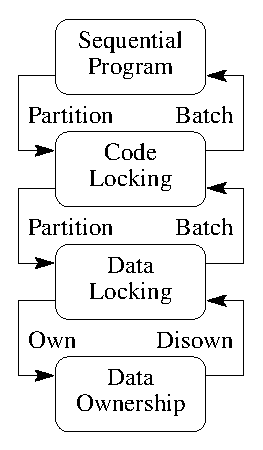
\includegraphics{SMPdesign/LockGranularity}
\end{center}
\caption{Design Patterns and Lock Granularity}
\label{fig:SMPdesign:Design Patterns and Lock Granularity}
\end{figure}

\subsection{Sequential Program}
\label{sec:SMPdesign:Sequential Program}

If the program runs fast enough on a single processor, and
has no interactions with other processes, threads, or interrupt
handlers, you should
remove the synchronization primitives and spare yourself their
overhead and complexity.
Some would argue that Moore's Law will eventually force all
programs into this category.
Others would disagree, particularly given the decrease in
% @@@ Intel Trademark
rate of CPU clock-frequency growth in Intel CPUs since the year 2003,
as can be seen in
Figure~\ref{fig:SMPdesign:Clock-Frequency Trend for Intel CPUs}.
The debate as to whether this leveling-off will result in single chips
with thousands
of CPUs will not be settled soon, but given that Paul is typing this
sentence on a dual-core laptop, the age of SMP does seem to be upon us.

\begin{figure}[htb]
\begin{center}
\resizebox{3in}{!}{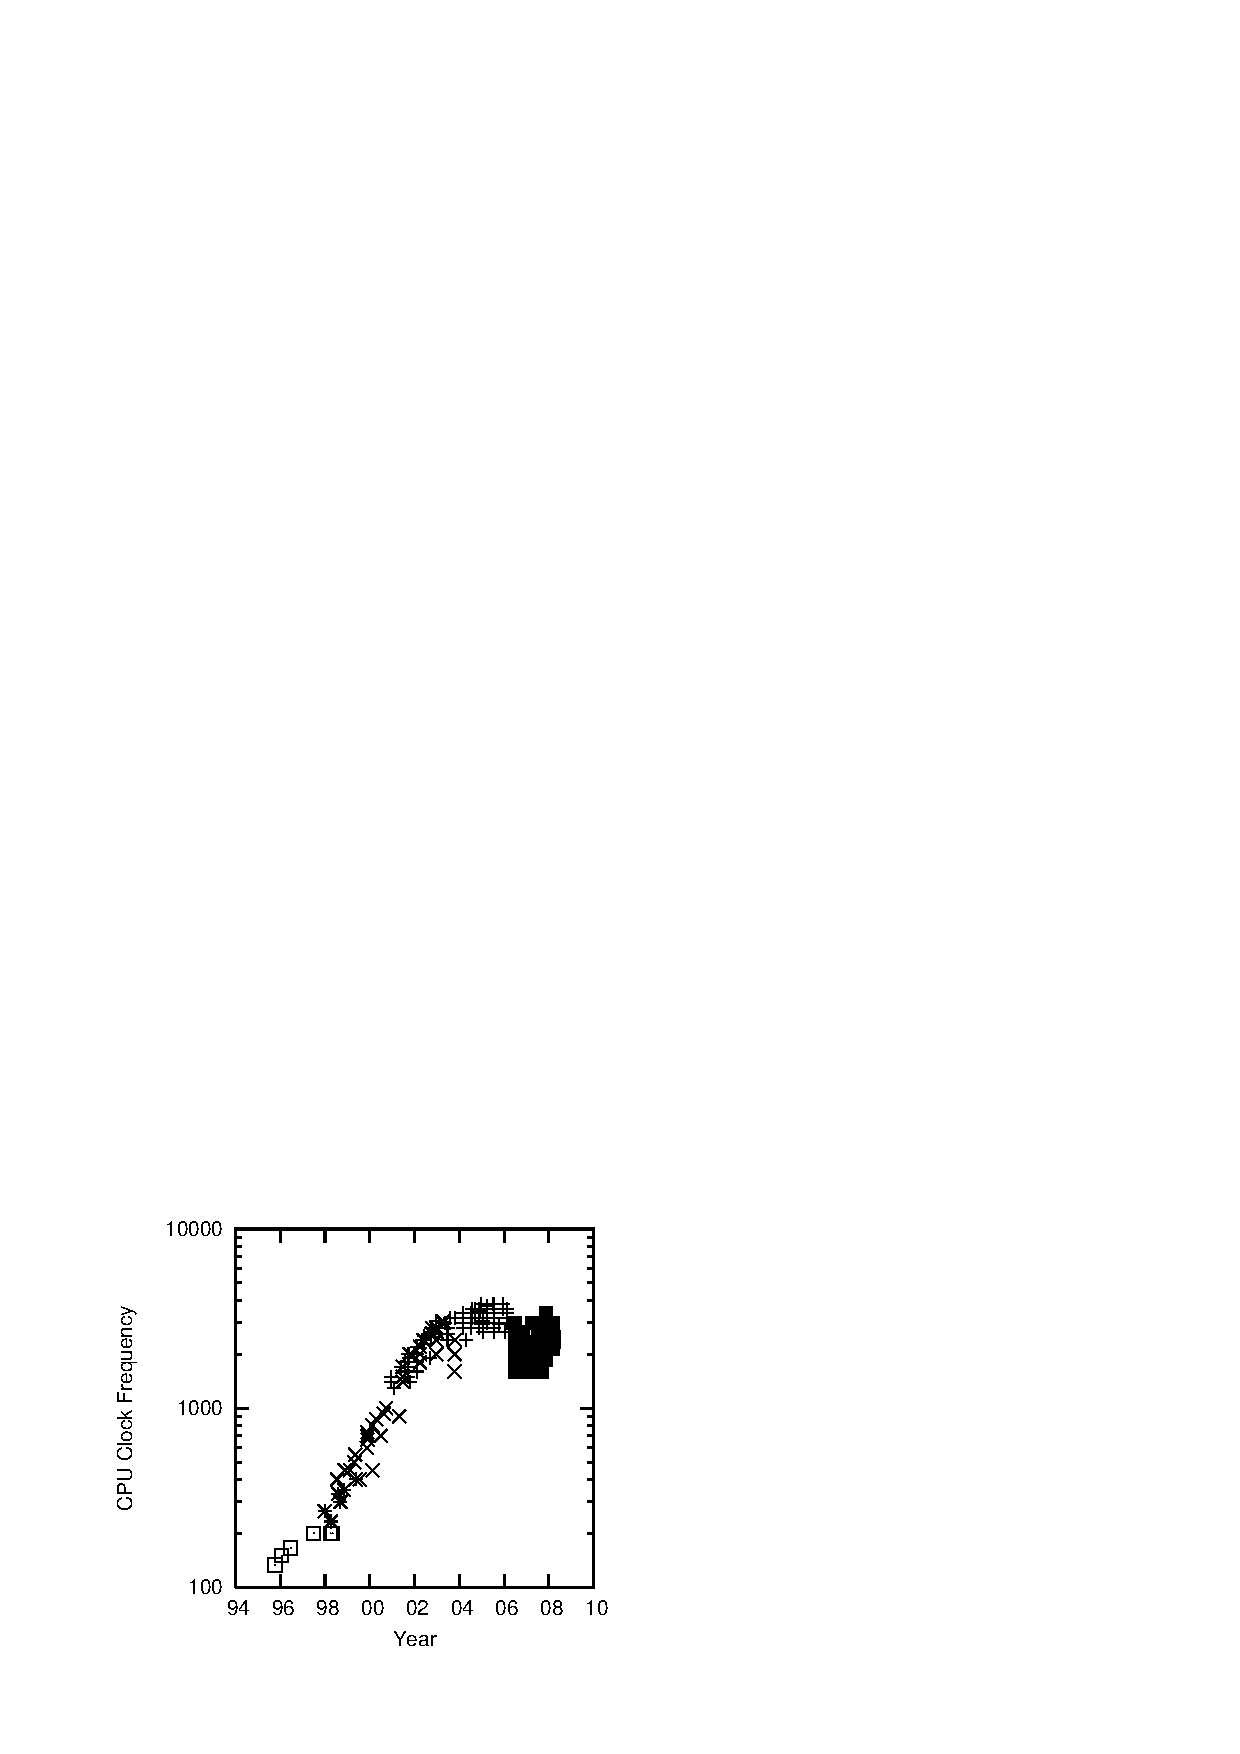
\includegraphics{SMPdesign/clockfreq}}
\end{center}
\caption{Clock-Frequency Trend for Intel CPUs}
\label{fig:SMPdesign:Clock-Frequency Trend for Intel CPUs}
\end{figure}

Please note that this does \emph{not} mean that you should code each
and every program in a multi-threaded manner.
Again, if a program runs quickly enough on a single processor,
spare yourself the overhead and complexity of SMP synchronization
primitives.
The simplicity of the hash-table lookup code in
Figure~\ref{fig:SMPdesign:Sequential-Program Hash Table Search}
underscores this point.\footnote{
	The examples in this section are taken from Hart et
	al.~\cite{ThomasEHart2006a}, adapted for clarity
	by gathering code related code from multiple files.}

\begin{figure}[htbp] 
{ \scriptsize
\begin{verbatim}
  1 struct hash_table
  2 {
  3   long nbuckets;
  4   struct node **buckets;
  5 };
  6 
  7 typedef struct node {
  8   unsigned long key;
  9   struct node *next;
 10 } node_t;
 11 
 12 int hash_search(struct hash_table *h, long key)
 13 {
 14   struct node *cur;
 15 
 16   cur = h->buckets[key % h->nbuckets];
 17   while (cur != NULL) {
 18     if (cur->key >= key) {
 19       return (cur->key == key);
 20     }
 21     cur = cur->next;
 22   }
 23   return 0;
 24 }
\end{verbatim}
}
\caption{Sequential-Program Hash Table Search}
\label{fig:SMPdesign:Sequential-Program Hash Table Search}
\end{figure}

% ./test_hash_null.exe 1000 0/100 1 1024 1
% ./test_hash_null.exe: nmilli: 1000 update/total: 0/100 nelements: 1 nbuckets: 1024 nthreads: 1
% ./test_hash_null.exe: avg = 96.2913  max = 98.2337  min = 90.4095  std = 2.95314
% ./test_hash_null.exe: nmilli: 1000 update/total: 0/100 nelements: 1 nbuckets: 1024 nthreads: 1
% ./test_hash_null.exe: avg = 91.5592  max = 97.3315  min = 89.9885  std = 2.88925
% ./test_hash_null.exe: nmilli: 1000 update/total: 0/100 nelements: 1 nbuckets: 1024 nthreads: 1
% ./test_hash_null.exe: avg = 93.3568  max = 106.162  min = 89.8828  std = 6.40418

On the other hand, if you are not in this happy situation, read on!

\subsection{Code Locking}
\label{sec:SMPdesign:Code Locking}

Code locking is the simplest locking design, using only
global locks.\footnote{
	If your program instead has locks in data structures,
	or, in the case of Java, uses classes with synchronized
	instances, you are instead using ``data locking'', described
	in Section~\ref{sec:SMPdesign:Data Locking}.}
It is especially
easy to retrofit an existing program to use code locking in
order to run it on a multiprocessor.  If the program has
only a single shared resource, code locking will even give
optimal performance.
However, many of the larger and more complex programs
require much of the execution to
occur in critical sections, which in turn causes code locking
to sharply limits their scalability.

Therefore, you should use code locking on programs that spend
only a small fraction of their execution time in critical sections or
from which only modest scaling is required.  In these cases,
code locking will provide a relatively simple program that is
very similar to its sequential counterpart,
as can be seen in
Figure~\ref{fig:SMPdesign:Code-Locking Hash Table Search}.
However, not that the simple return of the comparison in
\url{hash_search()} in
Figure~\ref{fig:SMPdesign:Sequential-Program Hash Table Search}
has now become three statements due to the need to release the
lock before returning.

\begin{figure}[htbp] 
{ \scriptsize
\begin{verbatim}
  1 spinlock_t hash_lock;
  2 
  3 struct hash_table
  4 {
  5   long nbuckets;
  6   struct node **buckets;
  7 };
  8 
  9 typedef struct node {
 10   unsigned long key;
 11   struct node *next;
 12 } node_t;
 13 
 14 int hash_search(struct hash_table *h, long key)
 15 {
 16   struct node *cur;
 17   int retval;
 18 
 19   spin_lock(&hash_lock);
 20   cur = h->buckets[key % h->nbuckets];
 21   while (cur != NULL) {
 22     if (cur->key >= key) {
 23       retval = (cur->key == key);
 24       spin_unlock(&hash_lock);
 25       return retval;
 26     }
 27     cur = cur->next;
 28   }
 29   spin_unlock(&hash_lock);
 30   return 0;
 31 }
\end{verbatim}
}
\caption{Code-Locking Hash Table Search}
\label{fig:SMPdesign:Code-Locking Hash Table Search}
\end{figure}

However, code locking is particularly prone to ``lock contention'',
where multiple CPUs need to acquire the lock concurrently.
SMP programmers who have taken care of groups of small children
(or of older people who are acting like children) will immediately
recognize the danger of having only one of something,
as illustrated in Figure~\ref{fig:SMPdesign:Lock Contention}.

% ./test_hash_codelock.exe 1000 0/100 1 1024 1
% ./test_hash_codelock.exe: nmilli: 1000 update/total: 0/100 nelements: 1 nbuckets: 1024 nthreads: 1
% ./test_hash_codelock.exe: avg = 164.115  max = 170.388  min = 161.659  std = 3.21857
% ./test_hash_codelock.exe: nmilli: 1000 update/total: 0/100 nelements: 1 nbuckets: 1024 nthreads: 1
% ./test_hash_codelock.exe: avg = 181.17  max = 198.4  min = 162.459  std = 15.8585
% ./test_hash_codelock.exe: nmilli: 1000 update/total: 0/100 nelements: 1 nbuckets: 1024 nthreads: 1
% ./test_hash_codelock.exe: avg = 167.651  max = 189.014  min = 162.144  std = 10.6819

% ./test_hash_codelock.exe 1000 0/100 1 1024 2
% ./test_hash_codelock.exe: nmilli: 1000 update/total: 0/100 nelements: 1 nbuckets: 1024 nthreads: 2
% ./test_hash_codelock.exe: avg = 378.481  max = 385.971  min = 374.235  std = 4.05934
% ./test_hash_codelock.exe: nmilli: 1000 update/total: 0/100 nelements: 1 nbuckets: 1024 nthreads: 2
% ./test_hash_codelock.exe: avg = 753.414  max = 1015.28  min = 377.734  std = 294.942
% ./test_hash_codelock.exe: nmilli: 1000 update/total: 0/100 nelements: 1 nbuckets: 1024 nthreads: 2
% ./test_hash_codelock.exe: avg = 502.737  max = 980.924  min = 374.406  std = 239.383

One solution to this problem, named ``data locking'', is described
in the next section.

\begin{figure}[htb]
\begin{center}
\resizebox{3in}{!}{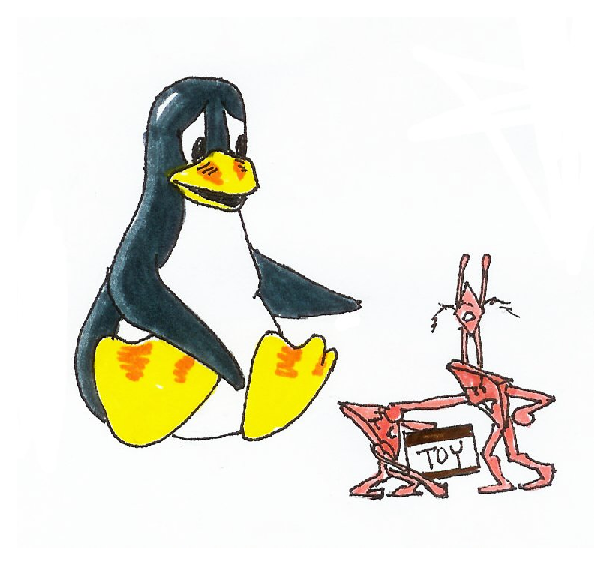
\includegraphics{cartoons/OneFighting}}
\end{center}
\caption{Lock Contention}
\label{fig:SMPdesign:Lock Contention}
\end{figure}

\subsection{Data Locking}
\label{sec:SMPdesign:Data Locking}

Many data structures may be partitioned,
with each partition of the data structure having its own lock.
Then the critical sections for each part of the data structure
can execute in parallel,
although only one instance of the critical section for a given
part could be executing at a given time.
Use data locking when contention must
be reduced, and where synchronization overhead is not
limiting speedups.
Data locking reduces contention by distributing the instances
of the overly-large critical section into multiple critical sections,
for example, maintaining per-hash-bucket critical sections in a
hash table, as shown in
Figure~\ref{fig:SMPdesign:Data-Locking Hash Table Search}.
The increased scalability again results in increased complexity
in the form of an additional data structure, the \url{struct} \url{bucket}.

\begin{figure}[htbp] 
{ \scriptsize
\begin{verbatim}
  1 struct hash_table
  2 {
  3   long nbuckets;
  4   struct bucket **buckets;
  5 };
  6 
  7 struct bucket {
  8   spinlock_t bucket_lock;
  9   node_t *list_head;
 10 };
 11 
 12 typedef struct node {
 13   unsigned long key;
 14   struct node *next;
 15 } node_t;
 16 
 17 int hash_search(struct hash_table *h, long key)
 18 {
 19   struct bucket *bp;
 20   struct node *cur;
 21   int retval;
 22 
 23   bp = h->buckets[key % h->nbuckets];
 24   spin_lock(&bp->bucket_lock);
 25   cur = bp->list_head;
 26   while (cur != NULL) {
 27     if (cur->key >= key) {
 28       retval = (cur->key == key);
 29       spin_unlock(&bp->hash_lock);
 30       return retval;
 31     }
 32     cur = cur->next;
 33   }
 34   spin_unlock(&bp->hash_lock);
 35   return 0;
 36 }
\end{verbatim}
}
\caption{Data-Locking Hash Table Search}
\label{fig:SMPdesign:Data-Locking Hash Table Search}
\end{figure}

In contrast with the contentious situation
shown in Figure~\ref{fig:SMPdesign:Lock Contention},
data locking helps promote harmony, as illustrated by
Figure~\ref{fig:SMPdesign:Data Locking} --- and in parallel programs,
this \emph{almost} always translates into increased performance and
scalability.
For this reason, data locking was heavily used by Sequent in
both its DYNIX and DYNIX/ptx operating
systems~\cite{Beck85,Inman85,Garg90,Dove90,McKenney92b,McKenney92a,McKenney93}.

\begin{figure}[htb]
\begin{center}
\resizebox{3in}{!}{\includegraphics{cartoons/ManyHappy}}
\end{center}
\caption{Data Locking}
\label{fig:SMPdesign:Data Locking}
\end{figure}

% ./test_hash_spinlock.exe 1000 0/100 1 1024 1
% ./test_hash_spinlock.exe: nmilli: 1000 update/total: 0/100 nelements: 1 nbuckets: 1024 nthreads: 1
% ./test_hash_spinlock.exe: avg = 158.118  max = 162.404  min = 156.199  std = 2.19391
% ./test_hash_spinlock.exe: nmilli: 1000 update/total: 0/100 nelements: 1 nbuckets: 1024 nthreads: 1
% ./test_hash_spinlock.exe: avg = 157.717  max = 162.446  min = 156.415  std = 2.36662
% ./test_hash_spinlock.exe: nmilli: 1000 update/total: 0/100 nelements: 1 nbuckets: 1024 nthreads: 1
% ./test_hash_spinlock.exe: avg = 158.369  max = 164.75  min = 156.501  std = 3.19454

% ./test_hash_spinlock.exe 1000 0/100 1 1024 2
% ./test_hash_spinlock.exe: nmilli: 1000 update/total: 0/100 nelements: 1 nbuckets: 1024 nthreads: 2
% ./test_hash_spinlock.exe: avg = 223.426  max = 422.948  min = 167.858  std = 100.136
% ./test_hash_spinlock.exe: nmilli: 1000 update/total: 0/100 nelements: 1 nbuckets: 1024 nthreads: 2
% ./test_hash_spinlock.exe: avg = 235.462  max = 507.134  min = 167.466  std = 135.836
% ./test_hash_spinlock.exe: nmilli: 1000 update/total: 0/100 nelements: 1 nbuckets: 1024 nthreads: 2
% ./test_hash_spinlock.exe: avg = 305.807  max = 481.685  min = 167.939  std = 132.589

However, as those how have taken care of small children can again attest,
even providing enough to go around is no guarantee of tranquillity.
The analogous situation can arise in SMP programs.
For example, the Linux kernel maintains a cache of files and directories
(called ``dcache'').
Each entry in this cache has its own lock, but the entries corresponding
to the root directory and its direct descendants are much more likely to
be traversed than are more obscure entries.
This can result in many CPUs contending for the locks of these popular
entries, resulting in a situation not unlike that
shown in Figure~\ref{fig:SMPdesign:Data and Skew}.

\begin{figure}[htb]
\begin{center}
\resizebox{3in}{!}{
\includegraphics{cartoons/ManyFighting}}
\end{center}
\caption{Data Locking and Skew}
\label{fig:SMPdesign:Data and Skew}
\end{figure}

In many cases, algorithms can be designed to reduce the instance of
data skew, and in some cases eliminate it entirely
(as appears to be possible with the Linux kernel's dcache~\cite{McKenney04a}).
Data locking is often used for partitionable data structures such as
hash tables, as well as in situations where multiple entities are each
represented by an instance of a given data structure.
The task list in version 2.6.17 of the Linux kernel is an example of the
latter, each task structure having its own \url{proc_lock}.

A key challenge with data locking on dynamically allocated structures
is ensuring that the structure remains in existence while the lock is
being acquired.
The code in
Figure~\ref{fig:SMPdesign:Data-Locking Hash Table Search}
finesses this challenge by placing the locks in the statically allocated
hash buckets, which are never freed.
However, this trick would not work if the hash table were resizeable,
so that the locks were now dynamically allocated.
In this case, there would need to be some means to prevent the hash
bucket from being freed during the time that its lock was being acquired.

\QuickQuiz{}
	What are some ways of preventing a structure from being freed while
	its lock is being acquired?
\QuickQuizAnswer{
	Here are a few possible solutions to this \emph{existence guarantee}
	problem:

	\begin{enumerate}
	\item	Provide a statically allocated lock that is held while
		the per-structure lock is being acquired, which is an
		example of hierarchical locking (see
		Section~\ref{sec:SMPdesign:Hierarchical Locking}).
		Of course, using a single global lock for this purpose
		can result in unacceptably high levels of lock contention,
		dramatically reducing performance and scalability.
	\item	Provide an array of statically allocated locks, hashing
		the structure's address to select the lock to be acquired,
		as described in Chapter~\ref{chp:Locking}.
		Given a hash function of sufficiently high quality, this
		avoids the scalability limitations of the single global
		lock, but in read-mostly situations, the lock-acquisition
		overhead can result in unacceptably degraded performance.
	\item	Use a garbage collector, in software environments providing
		them, so that a structure cannot be deallocated while being
		referenced.
		This works very well, removing the existence-guarantee
		burden (and much else besides) from the developer's
		shoulders, but imposes the overhead of garbage collection
		on the program.
		Although garbage-collection technology has advanced
		considerably in the past few decades, its overhead
		may be unacceptably high for some applications.
		In addition, some applications require that the developer
		exercise more control over the layout and placement of
		data structures than is permitted by most garbage collected
		environments.
	\item	Use \emph{hazard pointers}~\cite{MagedMichael04a}, which
		can be thought of as an inside-out reference count.
		Hazard-pointer-based algorithms maintain a per-thread list of
		pointers, so that the appearance of a given pointer on
		any of these lists acts as a reference to the corresponding
		structure.
		Hazard pointers are an interesting research direction, but
		have not yet seen much use in production (written in 2008).
	\item	Use transactional memory
		(TM)~\cite{Herlihy93a,DBLomet1977SIGSOFT,Shavit95},
		so that each reference and
		modification to the data structure in question is
		performed atomically.
		Although TM has engendered much excitement in recent years,
		and seems likely to be of some use in production software,
		developers should exercise some
		caution~\cite{McKenney2007PLOSTM}, particularly in
		performance-critical code.
	\item	Use RCU, which can be thought of as an extremely lightweight
		approximation to a garbage collector.
		Updaters are not permitted to free RCU-protected
		data structures that RCU readers might still be referencing.
		RCU is most heavily used for read-mostly data structures,
		and is discussed at length in
		Chapter~\ref{chp:defer:Deferred Processing}.
	\end{enumerate}

	For more on providing existence guarantees, see
	Chapters~\ref{chp:Locking} and \ref{chp:defer:Deferred Processing}.
} \QuickQuizEnd

\subsection{Data Ownership}
\label{sec:SMPdesign:Data Ownership}

Data ownership partitions a given data structure over the threads
or CPUs, so that each thread/CPU accesses its subset of the data
structure without any synchronization overhead whatsoever.
However, if one thread wishes to access some other thread's data,
the first thread is unable to do so directly.
Instead, the first thread must communicate with the second thread,
so that the second thread performs the operation on behalf of the
first, or, alternatively, migrates the data to the first thread.

Data ownership might seem arcane, but it is used very frequently:
\begin{enumerate}
\item	Any variables accessible by only one CPU or thread
	(such as {\tt auto} variables in C
	and C++) are owned by that CPU or process.
\item	An instance of a user interface owns the corresponding
	user's context.  It is very common for applications
	interacting with parallel database engines to be
	written as if they were entirely sequential programs.
	Such applications own the user interface and his current
	action.  Explicit parallelism is thus confined to the
	database engine itself.
\item	Parametric simulations are often trivially parallelized
	by granting each thread ownership of a particular region
	of the parameter space.
\end{enumerate}

If there is significant sharing, communication between the threads
or CPUs can result in significant complexity and overhead.
Furthermore, if the most-heavily used data happens to be that owned
by a single CPU, that CPU will be a ``hot spot'', sometimes with
results resembling that shown in Figure~\ref{fig:SMPdesign:Data and Skew}.
However, in situations where no sharing is required, data ownership
achieves ideal performance, and with code that can be as simple
as the sequential-program case shown in
Figure~\ref{fig:SMPdesign:Sequential-Program Hash Table Search}.
Such situations are often referred to as ``embarassingly
parallel'', and, in the best case, resemble the situation
previously shown in Figure~\ref{fig:SMPdesign:Data Locking}.

% ./test_hash_null.exe 1000 0/100 1 1024 1
% ./test_hash_null.exe: nmilli: 1000 update/total: 0/100 nelements: 1 nbuckets: 1024 nthreads: 1
% ./test_hash_null.exe: avg = 96.2913  max = 98.2337  min = 90.4095  std = 2.95314
% ./test_hash_null.exe: nmilli: 1000 update/total: 0/100 nelements: 1 nbuckets: 1024 nthreads: 1
% ./test_hash_null.exe: avg = 91.5592  max = 97.3315  min = 89.9885  std = 2.88925
% ./test_hash_null.exe: nmilli: 1000 update/total: 0/100 nelements: 1 nbuckets: 1024 nthreads: 1
% ./test_hash_null.exe: avg = 93.3568  max = 106.162  min = 89.8828  std = 6.40418

% ./test_hash_null.exe 1000 0/100 1 1024 2
% ./test_hash_null.exe: nmilli: 1000 update/total: 0/100 nelements: 1 nbuckets: 1024 nthreads: 2
% ./test_hash_null.exe: avg = 45.4526  max = 46.4281  min = 45.1954  std = 0.487791
% ./test_hash_null.exe: nmilli: 1000 update/total: 0/100 nelements: 1 nbuckets: 1024 nthreads: 2
% ./test_hash_null.exe: avg = 46.0238  max = 49.2861  min = 45.1852  std = 1.63127
% ./test_hash_null.exe: nmilli: 1000 update/total: 0/100 nelements: 1 nbuckets: 1024 nthreads: 2
% ./test_hash_null.exe: avg = 46.6858  max = 52.6278  min = 45.1761  std = 2.97102

Another important instance of data ownership occurs when the data
is read-only, in which case,
all threads can ``own'' it via replication.

\subsection{Locking Granularity and Performance}
\label{sec:SMPdesign:Locking Granularity and Performance}

\emph{@@@ summarize performance and scalability here, once
we get clean performance numbers.}

\section{Parallel Fastpath}
\label{sec:SMPdesign:Parallel Fastpath}

Fine-grained (and therefore \emph{usually} higher-performance)
designs are typically more complex than are coarser-grained designs.
In many cases, most of the overhead is incurred by a small fraction
of the code~\cite{Knuth73}.
So why not focus effort on that small fraction?

This is the idea behind the parallel-fastpath design pattern, to aggressively
parallelize the common-case code path without incurring the complexity
that would be required to aggressively parallelize the entire algorithm.
You must understand not only the specific algorithm you wish
to parallelize, but also the workload that the algorithm will
be subjected to.  Great creativity and design
effort is often required to construct a parallel fastpath.

Parallel fastpath combines different patterns (one for the 
fastpath, one elsewhere) and is therefore a template pattern.
The following instances of parallel
fastpath occur often enough to warrant their own patterns,
as depicted in Figure~\ref{fig:SMPdesign:Parallel-Fastpath Design Patterns}:

\begin{figure}[htb]
\begin{center}
% \resizebox{3in}{!}{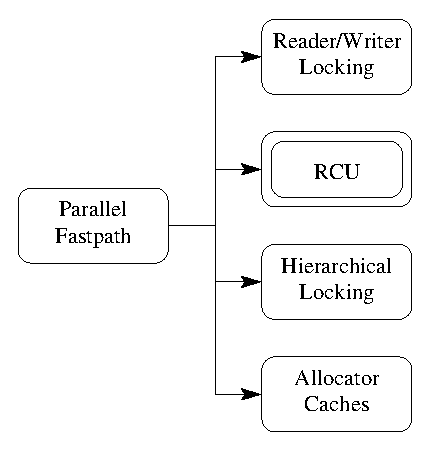
\includegraphics{SMPdesign/ParallelFastpath}}
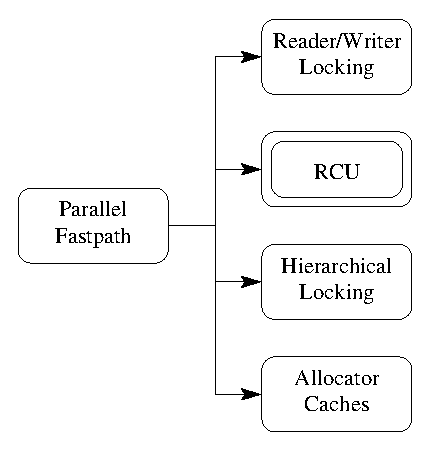
\includegraphics{SMPdesign/ParallelFastpath}
\end{center}
\caption{Parallel-Fastpath Design Patterns}
\label{fig:SMPdesign:Parallel-Fastpath Design Patterns}
\end{figure}

\begin{enumerate}
\item	Reader/Writer Locking
	(described below in Section~\ref{sec:SMPdesign:Reader/Writer Locking}).
\item	Read-copy update (RCU), which is very briefly described below
	in Section~\ref{sec:defer:Read-Copy Update (RCU)}).
\item   Hierarchical Locking~(\cite{McKenney95b}).
\item	Resource Allocator Caches~(\cite{McKenney95b,McKenney93}).
	See Chapter~\ref{chp:Memory Allocation} for more detail.
\end{enumerate}

\subsection{Reader/Writer Locking}
\label{sec:SMPdesign:Reader/Writer Locking}

If synchronization overhead is negligible (for example, if the program
uses coarse-grained parallelism), and if only a small fraction of the
critical sections modify data, then allowing multiple readers
to proceed in parallel can greatly increase scalability.
Writers exclude both readers and each other.
Figure~\ref{fig:SMPdesign:Reader-Writer-Locking Hash Table Search}
shows how the hash search might be implemented using reader-writer locking.

\begin{figure}[htbp] 
{ \scriptsize
\begin{verbatim}
  1 rwlock_t hash_lock;
  2 
  3 struct hash_table
  4 {
  5   long nbuckets;
  6   struct node **buckets;
  7 };
  8 
  9 typedef struct node {
 10   unsigned long key;
 11   struct node *next;
 12 } node_t;
 13 
 14 int hash_search(struct hash_table *h, long key)
 15 {
 16   struct node *cur;
 17   int retval;
 18 
 19   read_lock(&hash_lock);
 20   cur = h->buckets[key % h->nbuckets];
 21   while (cur != NULL) {
 22     if (cur->key >= key) {
 23       retval = (cur->key == key);
 24       read_unlock(&hash_lock);
 25       return retval;
 26     }
 27     cur = cur->next;
 28   }
 29   read_unlock(&hash_lock);
 30   return 0;
 31 }
\end{verbatim}
}
\caption{Reader-Writer-Locking Hash Table Search}
\label{fig:SMPdesign:Reader-Writer-Locking Hash Table Search}
\end{figure}

Reader/writer locking is a simple instance of asymmetric locking.
Snaman~\cite{Snaman87} describes a more ornate six-mode
asymmetric locking design used in several clustered systems.
Locking in general and reader-writer locking in particular is described
extensively in
Chapter~\ref{chp:Locking}.

\subsection{Read-Copy Update Introduction}
\label{sec:SMPdesign:Read-Copy Update Introduction}

Read-copy update (RCU) is a mutual-exclusion mechanism which can be
used as an alternative to reader-writer locking.
RCU features extremely low-overhead wait-free read-side critical sections,
however, updates can be expensive, as they must leave old versions of the
data structure in place for the sake of pre-existing readers.
These old versions may be reclaimed once all such pre-existing readers
complete their accesses.~\cite{WikipediaRCU}.

It turns out that our example hash-search program is well-suited to RCU.
Other programs may be more difficult to adapt to RCU,
and more detail on such adaptation may be found in
Section~\ref{sec:defer:Read-Copy Update (RCU)}.

In some implementations of RCU
(such as that of Hart et al.~\cite{ThomasEHart2006a}),
the search code can be implemented
exactly as in sequential programs, as was shown in
Figure~\ref{fig:SMPdesign:Sequential-Program Hash Table Search}.
However, other environments, including the Linux kernel, require
that the RCU read-side critical sections be marked explicitly,
as shown in
Figure~\ref{fig:SMPdesign:RCU Hash Table Search}.
Such marking can be a great favor to whoever must later read the code!

\begin{figure}[htbp] 
{ \scriptsize
\begin{verbatim}
  1 struct hash_table
  2 {
  3   long nbuckets;
  4   struct node **buckets;
  5 };
  6 
  7 typedef struct node {
  8   unsigned long key;
  9   struct node *next;
 10 } node_t;
 11 
 12 int hash_search(struct hash_table *h, long key)
 13 {
 14   struct node *cur;
 15   int retval;
 16 
 17   rcu_read_lock();
 18   cur = h->buckets[key % h->nbuckets];
 19   while (cur != NULL) {
 20     if (cur->key >= key) {
 21       retval = (cur->key == key);
 22       rcu_read_unlock();
 23       return retval;
 24     }
 25     cur = cur->next;
 26   }
 27   rcu_read_unlock();
 28   return 0;
 29 }
\end{verbatim}
}
\caption{RCU Hash Table Search}
\label{fig:SMPdesign:RCU Hash Table Search}
\end{figure}

Update-side code must wait for a ``grace period'' after removing an
element before freeing it, and RCU implementations provide special
primitives for this purpose.
For example, the Linux kernel provides \url{synchronize_rcu()} to
block until the end of a subsequent grace period (and other related primitives
as well),
while Hart et al.~\cite{ThomasEHart2006a} provide a \url{free_node_later()}
primitive that frees the specified data element after the end of a
subsequent grace period (in contrast to their \url{free_node()} primitive
that immediately frees the specified data element).

RCU's greatest strength is its low-overhead (in some cases, zero-overhead)
read-side primitives.
In many implementations, these primitives are in fact deterministic,
which is useful in realtime environments.

\subsection{Hierarchical Locking}
\label{sec:SMPdesign:Hierarchical Locking}

The idea behind hierarchical locking is to have a coarse-grained lock
that is held only long enough to work out which fine-grained lock
to acquire.
Figure~\ref{fig:SMPdesign:Hierarchical-Locking Hash Table Search}
shows how our hash-table search might be adapted to do hierarchical
locking, but also shows the great weakness of this approach:
we have paid the overhead of acquiring a second lock, but we only
hold it for a short time.
In this case, the simpler data-locking approach would be simpler
and likely perform better.

\begin{figure}[htbp] 
{ \scriptsize
\begin{verbatim}
  1 struct hash_table
  2 {
  3   long nbuckets;
  4   struct bucket **buckets;
  5 };
  6 
  7 struct bucket {
  8   spinlock_t bucket_lock;
  9   node_t *list_head;
 10 };
 11 
 12 typedef struct node {
 13   spinlock_t node_lock;
 14   unsigned long key;
 15   struct node *next;
 16 } node_t;
 17 
 18 int hash_search(struct hash_table *h, long key)
 19 {
 20   struct bucket *bp;
 21   struct node *cur;
 22   int retval;
 23 
 24   bp = h->buckets[key % h->nbuckets];
 25   spin_lock(&bp->bucket_lock);
 26   cur = bp->list_head;
 27   while (cur != NULL) {
 28     if (cur->key >= key) {
 29       spin_lock(&cur->node_lock);
 30       spin_unlock(&bp->bucket_lock);
 31       retval = (cur->key == key);
 32       spin_unlock(&cur->node_lock);
 33       return retval;
 34     }
 35     cur = cur->next;
 36   }
 37   spin_unlock(&bp->bucket_lock);
 38   return 0;
 39 }
\end{verbatim}
}
\caption{Hierarchical-Locking Hash Table Search}
\label{fig:SMPdesign:Hierarchical-Locking Hash Table Search}
\end{figure}

\QuickQuiz{}
	In what situation would hierarchical locking work well?
\QuickQuizAnswer{
	If the comparison on line~31 of
	Figure~\ref{fig:SMPdesign:Hierarchical-Locking Hash Table Search}
	were replaced by a much heavier-weight operation,
	then releasing {\tt bp->bucket\_lock} \emph{might} reduce lock
	contention enough to outweigh the overhead of the extra
	acquisition and release of {\tt cur->node\_lock}.
} \QuickQuizEnd

\subsection{Resource Allocator Caches}
\label{sec:SMPdesign:Resource Allocator Caches}

This section presents a simplified schematic of a parallel fixed-block-size
memory allocator.
More detailed descriptions may be found in the
literature~\cite{McKenney92a,McKenney93,Bonwick01slab,McKenney01e}
or in the Linux kernel~\cite{Torvalds2.6kernel}.

\subsubsection{Parallel Resource Allocation Problem}

The basic problem facing a parallel memory allocator is the tension
between the need to provide extremely fast memory allocation and
freeing in the common case and the need to efficiently distribute
memory in face of unfavorable allocation and freeing patterns.

To see this tension, consider a straightforward application of
data ownership to this problem --- simply carve up memory so that
each CPU owns its share.
For example, suppose that a system with two CPUs has two gigabytes
of memory (such as the one that I am typing on right now).
We could simply assign each CPU one gigabyte of memory, and allow
each CPU to access its own private chunk of memory, without the
need for locking and its complexities and overheads.
Unfortunately, this simple scheme breaks down if an algorithm happens
to have CPU 0 allocate all of the memory and CPU 1 the free it, as
would happen in a simple producer-consumer workload.

The other extreme, code locking, suffers from excessive lock contention
and overhead~\cite{McKenney93}.

\subsubsection{Parallel Fastpath for Resource Allocation}

The commonly used solution uses parallel fastpath with each CPU
owning a modest cache of blocks, and with a large code-locked
shared pool for additional blocks.
To prevent any given CPU from monopolizing the memory blocks,
we place a limit on the number of blocks that can be in each CPU's
cache.
In a two-CPU system, the flow of memory blocks will be as shown
in Figure~\ref{fig:SMPdesign:Allocator Cache Schematic}:
when a given CPU is trying to free a block when its pool is full,
it sends blocks to the global pool, and, similarly, when that CPU
is trying to allocate a block when its pool is empty, it retrieves
blocks from the global pool.

\begin{figure}[htb]
\begin{center}
\resizebox{3in}{!}{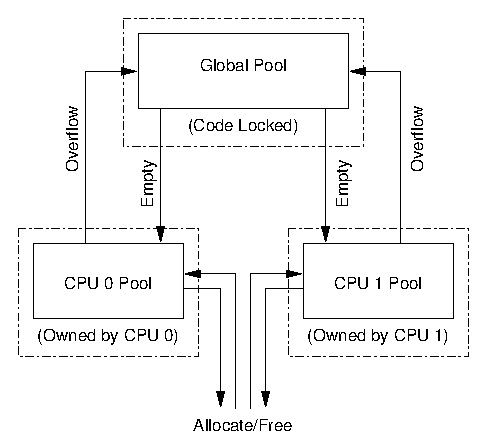
\includegraphics{SMPdesign/allocatorcache}}
\end{center}
\caption{Allocator Cache Schematic}
\label{fig:SMPdesign:Allocator Cache Schematic}
\end{figure}

\subsubsection{Data Structures}

The actual data structures for a ``toy'' implementation of allocator
caches are shown in
Figure~\ref{fig:SMPdesign:Allocator-Cache Data Structures}.
The ``Global Pool'' of Figure~\ref{fig:SMPdesign:Allocator Cache Schematic}
is implemented by \url{globalmem} of type \url{struct globalmempool},
and the two CPU pools by the per-CPU variable \url{percpumem} of
type \url{percpumempool}.
Both of these data structures have arrays of pointers to blocks
in their \url{pool} fields, which are filled from index zero upwards.
Thus, if \url{globalmem.pool[3]} is \url{NULL}, then the remainder of
the array from index 4 up must also be NULL.
The \url{cur} fields contain the index of the highest-numbered full
element of the \url{pool} array, or -1 if all elements are empty.
All elements from \url{globalmem.pool[0]} through
\url{globalmem.pool[globalmem.cur]} must be full, and all the rest
must be empty.\footnote{
	Both pool sizes (\url{TARGET_POOL_SIZE} and
	\url{GLOBAL_POOL_SIZE}) are unrealistically small, but this small
	size makes it easier to single-step the program in order to get
	a feel for its operation.}

\begin{figure}[htbp] 
{ \scriptsize
\begin{verbatim}
  1 #define TARGET_POOL_SIZE 3
  2 #define GLOBAL_POOL_SIZE 40
  3 
  4 struct globalmempool {
  5   spinlock_t mutex;
  6   int cur;
  7   struct memblock *pool[GLOBAL_POOL_SIZE];
  8 } globalmem;
  9 
 10 struct percpumempool {
 11   int cur;
 12   struct memblock *pool[2 * TARGET_POOL_SIZE];
 13 };
 14 
 15 DEFINE_PER_THREAD(struct percpumempool, percpumem);
\end{verbatim}
}
\caption{Allocator-Cache Data Structures}
\label{fig:SMPdesign:Allocator-Cache Data Structures}
\end{figure}

The operation of the pool data structures is illustrated by
Figure~\ref{fig:SMPdesign:Allocator Pool Schematic},
with the six boxes representing the array of pointers making up
the \url{pool} field, and the number preceding them representing
the \url{cur} field.
The shaded boxes represent non-\url{NULL} pointers, while the empty
boxes represent \url{NULL} pointers.
An important, though potentially confusing, invariant of this
data structure is that the \url{cur} field is always one
smaller than the number of non-\url{NULL} pointers.

\begin{figure}[htb]
\begin{center}
\resizebox{3in}{!}{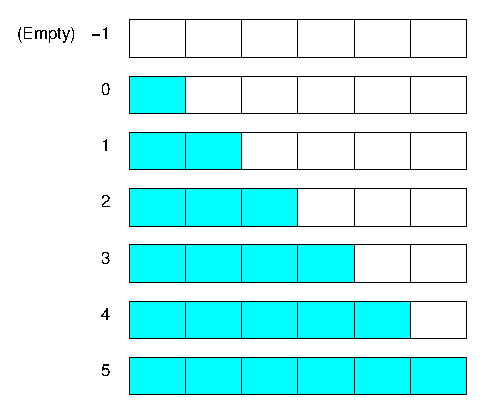
\includegraphics{SMPdesign/AllocatorPool}}
\end{center}
\caption{Allocator Pool Schematic}
\label{fig:SMPdesign:Allocator Pool Schematic}
\end{figure}

\subsubsection{Allocation Function}

The allocation function \url{memblock_alloc()} may be seen in
Figure~\ref{fig:SMPdesign:Allocator-Cache Allocator Function}.
Line~7 picks up the current thread's per-thread pool,
and line~8 check to see if it is empty.

If so, lines~9-16 attempt to refill it from the global pool
under the spinlock acquired on line~9 and released on line~16.
Lines~10-14 move blocks from the global to the per-thread pool until
either the local pool reaches its target size (half full) or
the global pool is exhausted, and line~15 sets the per-thread pool's
count to the proper value.

In either case, line~18 checks for the per-thread pool still being
empty, and if not, lines~19-21 remove a block and return it.
Otherwise, line~23 tells the sad tale of memory exhaustion.

\begin{figure}[htbp] 
{ \scriptsize
\begin{verbatim}
  1 struct memblock *memblock_alloc(void)
  2 {
  3   int i;
  4   struct memblock *p;
  5   struct percpumempool *pcpp;
  6
  7   pcpp = &__get_thread_var(percpumem);
  8   if (pcpp->cur < 0) {
  9     spin_lock(&globalmem.mutex);
 10     for (i = 0; i < TARGET_POOL_SIZE &&
 11                 globalmem.cur >= 0; i++) {
 12       pcpp->pool[i] = globalmem.pool[globalmem.cur];
 13       globalmem.pool[globalmem.cur--] = NULL;
 14     }
 15     pcpp->cur = i - 1;
 16     spin_unlock(&globalmem.mutex);
 17   }
 18   if (pcpp->cur >= 0) {
 19     p = pcpp->pool[pcpp->cur];
 20     pcpp->pool[pcpp->cur--] = NULL;
 21     return p;
 22   }
 23   return NULL;
 24 }
\end{verbatim}
}
\caption{Allocator-Cache Allocator Function}
\label{fig:SMPdesign:Allocator-Cache Allocator Function}
\end{figure}

\subsubsection{Free Function}

Figure~\ref{fig:SMPdesign:Allocator-Cache Free Function} shows
the memory-block free function.
Line~6 gets a pointer to this thread's pool, and
line~7 checks to see if this per-thread pool is full.

If so, lines~8-15 empty half of the per-thread pool into the global pool,
with lines~8 and 14 acquiring and releasing the spinlock.
Lines~9-12 implement the loop moving blocks from the local to the
global pool, and line~13 sets the per-thread pool's count to the proper
value.

In either case, line~16 then places the newly freed block into the
per-thread pool.

\begin{figure}[htbp] 
{ \scriptsize
\begin{verbatim}
  1 void memblock_free(struct memblock *p)
  2 {
  3   int i;
  4   struct percpumempool *pcpp;
  5 
  6   pcpp = &__get_thread_var(percpumem);
  7   if (pcpp->cur >= 2 * TARGET_POOL_SIZE - 1) {
  8     spin_lock(&globalmem.mutex);
  9     for (i = pcpp->cur; i >= TARGET_POOL_SIZE; i--) {
 10       globalmem.pool[++globalmem.cur] = pcpp->pool[i];
 11       pcpp->pool[i] = NULL;
 12     }
 13     pcpp->cur = i;
 14     spin_unlock(&globalmem.mutex);
 15   }
 16   pcpp->pool[++pcpp->cur] = p;
 17 }
\end{verbatim}
}
\caption{Allocator-Cache Free Function}
\label{fig:SMPdesign:Allocator-Cache Free Function}
\end{figure}

\subsubsection{Performance}

Rough performance results\footnote{
	This data was not collected in a statistically meaningful way,
	and therefore should be viewed with great skepticism and suspicion.
	Good data-collection and -reduction practice is discussed
	in Chapter @@@.
	That said, repeated runs gave similar results, and these results
	match more careful evaluations of similar algorithms.}
are shown in
Figure~\ref{fig:SMPdesign:Allocator Cache Performance},
running on a dual-core Intel x86 running at 1GHz (4300 bogomips per CPU)
with at most six blocks allowed in each CPU's cache.
In this micro-benchmark,
each thread repeated allocates a group of blocks and then frees it, with
the size of the group being the ``allocation run length'' displayed on
the x-axis.
The y-axis shows the number of successful allocation/free pairs per
microsecond --- failed allocations are not counted.
The ``X''s are from a two-thread run, while the ``+''s are from a
single-threaded run.

\begin{figure}[htb]
\begin{center}
\resizebox{3in}{!}{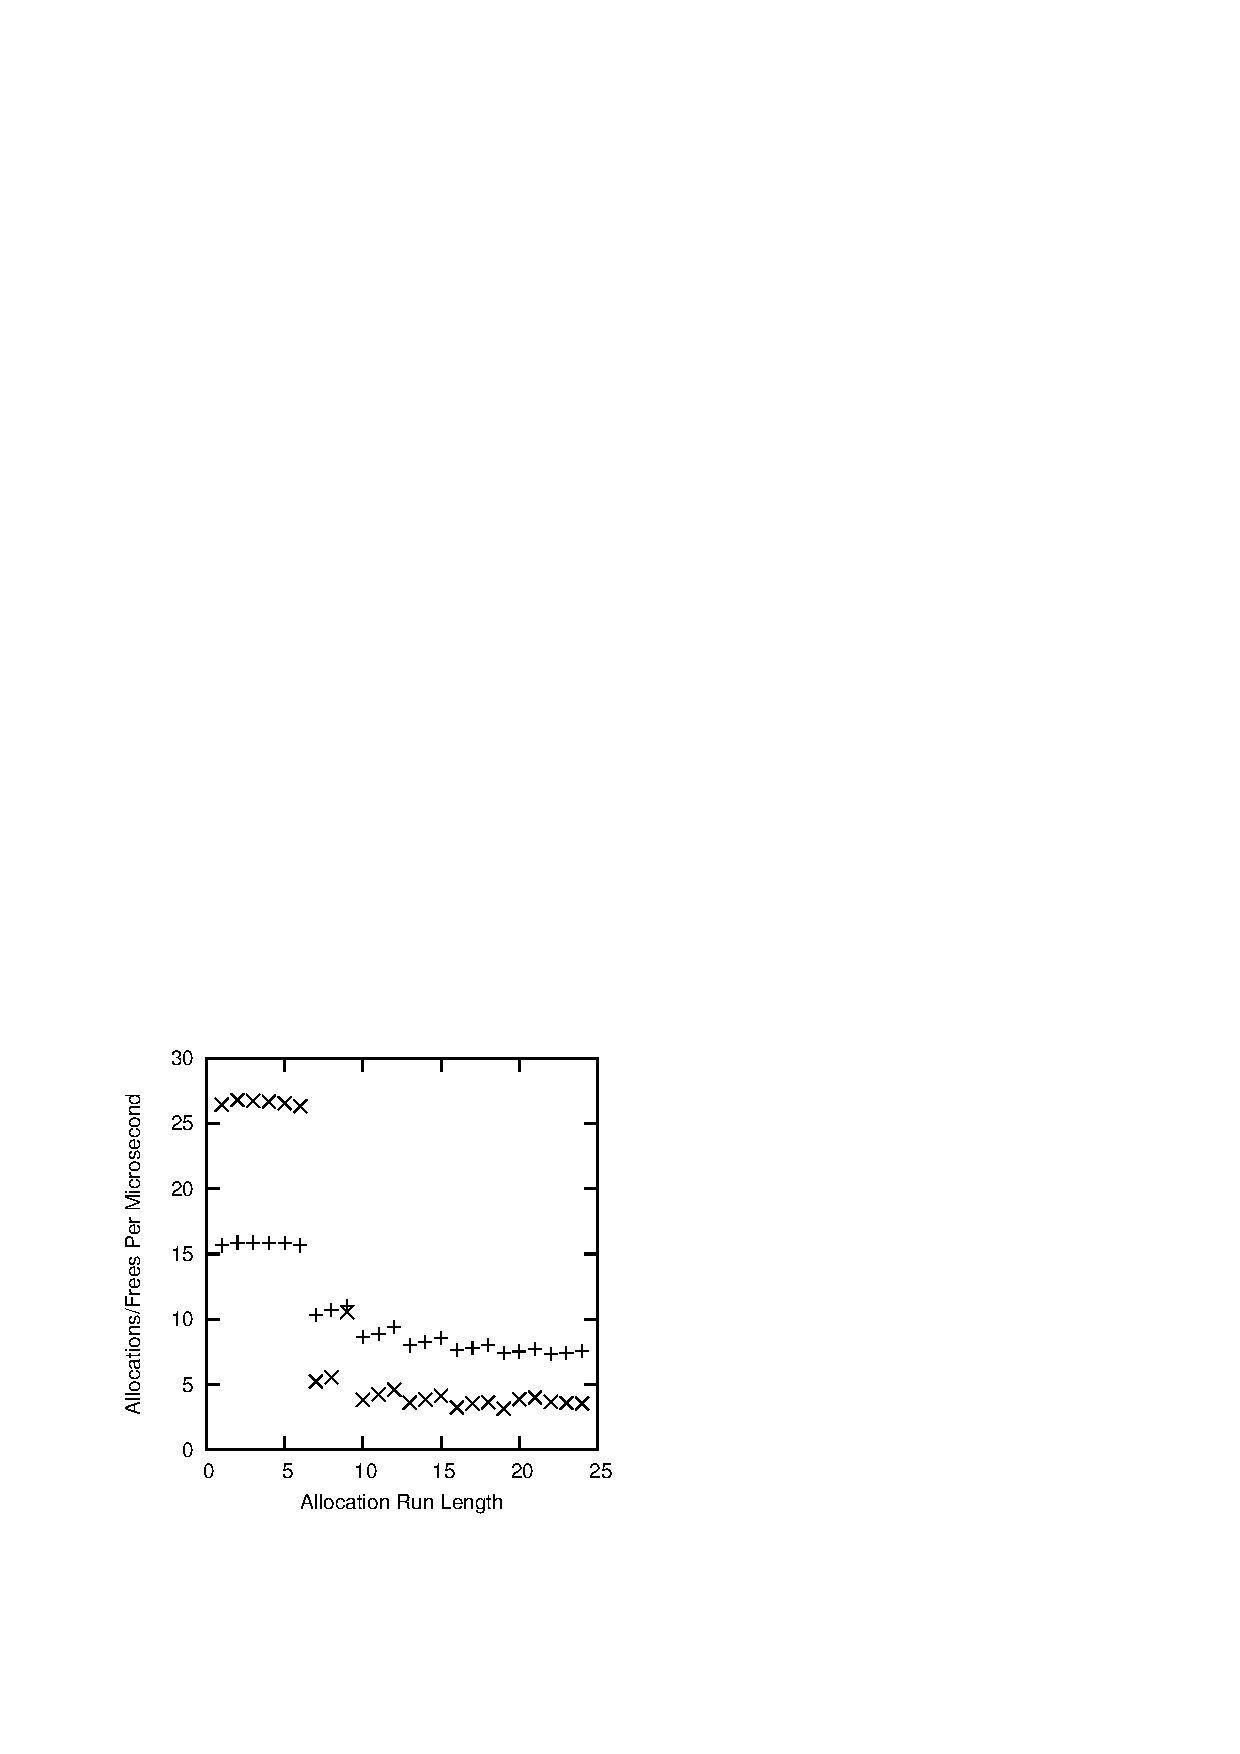
\includegraphics{SMPdesign/smpalloc}}
\end{center}
\caption{Allocator Cache Performance}
\label{fig:SMPdesign:Allocator Cache Performance}
\end{figure}

Note that run lengths up to six scale linearly and give excellent performance,
while run lengths greater than six show poor performance and almost always
also show \emph{negative} scaling.
It is therefore quite important to size \url{TARGET_POOL_SIZE}
sufficiently large,
which fortunately is usually quite easy to do in actual
practice~\cite{McKenney01e}, especially given today's large memories.
For example, in most systems, it is quite reasonable to set
\url{TARGET_POOL_SIZE} to 100, in which case allocations and frees
are guaranteed to be confined to per-thread pools at least 99\% of
the time.

As can be seen from the figure, the situations where the common-case
data-ownership applies (run lengths up to six) provide greatly improved
performance compared to the cases where locks must be acquired.
Avoiding locking in the common case will be a recurring theme through
this book.

\QuickQuiz{}
	In Figure~\ref{fig:SMPdesign:Allocator Cache Performance},
	there is a pattern of performance rising with increasing run
	length in groups of three samples, for example, for run lengths
	10, 11, and 12.
	Why?
\QuickQuizAnswer{
	This is due to the per-CPU target value being three.
	A run length of 12 must acquire the global-pool lock twice,
	while a run length of 13 must acquire the global-pool lock
	three times.
} \QuickQuizEnd

\QuickQuiz{}
	Allocation failures were observed in the two-thread
	tests at run lengths of 19 and greater.
	Given the global-pool size of 40 and the per-CPU target
	pool size of three, what is the smallest allocation run
	length at which failures can occur?
\QuickQuizAnswer{
	The exact solution to this problem is left as an exercise to
	the reader.
	The first solution received will be credited to its submitter.
	As a rough rule of thumb, the global pool size should be at least
	$m+2sn$, where
	``m'' is the maximum number of elements allocated at a given time,
	``s'' is the per-CPU pool size,
	and ``n'' is the number of CPUs.
} \QuickQuizEnd

\subsubsection{Real-World Design}

The toy parallel resource allocator was quite simple, but real-world
designs expand on this approach in a number of ways.

First, real-world allocators are required to handle a wide range
of allocation sizes, as opposed to the single size shown in this
toy example.
One popular way to do this is to offer a fixed set of sizes, spaced
so as to balance external and internal fragmentation, such as in
the late-1980s BSD memory allocator~\cite{McKusick88}.
Doing this would mean that the ``globalmem'' variable would need
to be replicated on a per-size basis, and that the associated
lock would similarly be replicated, resulting in data locking
rather than the toy program's code locking.

Second, production-quality systems must be able to repurpose memory,
meaning that they must be able to coalesce blocks into larger structures,
such as pages~\cite{McKenney93}.
This coalescing will also need to be protected by a lock, which again
could be replicated on a per-size basis.

Third, coalesced memory must be returned to the underlying memory
system, and pages of memory must also be allocated from the underlying
memory system.
The locking required at this level will depend on that of the underlying
memory system, but could well be code locking.
Code locking can often be tolerated at this level, because this
level is so infrequently reached in well-designed systems~\cite{McKenney01e}.

Despite this real-world design's greater complexity, the underlying
idea is the same --- repeated application of parallel fastpath,
as shown in
Table~\ref{fig:app:questions:Schematic of Real-World Parallel Allocator}.

\begin{table}[htbp]
{ \scriptsize
\begin{tabular}{l|l|p{1in}}
Level	& Locking & Purpose \\
\hline
Per-thread pool	  & Data ownership & High-speed allocation \\
Global block pool & Data locking   & Distributing blocks among threads \\
Coalescing	  & Data locking   & Combining blocks into pages \\
System memory	  & Code locking   & Memory from/to system \\
\end{tabular}
}
\caption{Schematic of Real-World Parallel Allocator}
\label{fig:app:questions:Schematic of Real-World Parallel Allocator}
\end{table}

\section{Performance Summary}
\label{Performance Summary}

\emph{@@@ summarize performance of the various options.
Forward-reference to the RCU/NBS section.}

% locking/locking.tex

\QuickQuizChapter{chp:Locking}{Locking}

The role of villain in much of the past few decades' concurrency research
literature is played by locking,
which stands accused of promoting deadlocks, convoying, starvation,
unfairness, data races, and all manner of other concurrency sins.
Interestingly enough, the role of workhorse in production-quality
shared-memory parallel software is played by, you guessed it, locking.

There are a number of reasons behind this dichotomy:

\begin{enumerate}
\item	Many of locking's sins have pragmatic design solutions that
	work well in most cases, for example:
	\begin{enumerate}
	\item	Use of lock hierarchies to avoid deadlock.
	\item	Deadlock-detection tools, for example, the Linux kernel's
		lockdep facility~\cite{JonathanCorbet2006lockdep}.
	\item	Locking-friendly data structures, such as
		arrays, hash tables, and radix trees, which will
		be covered in Chapter~\ref{chp:Data Structures}.
	\end{enumerate}
\item	Some of locking's sins are problems only at high levels of
	contention, levels reached only by poorly designed programs.
\item	Some of locking's sins are avoided by using other synchronization
	mechanisms in concert with locking.
	These other mechanisms include reference counters,
	statistical counters, simple non-blocking data structures, and RCU.
\item	Until quite recently, almost all large shared-memory parallel
	programs were developed in secret, so that it was difficult for
	most researchers to learn of these pragmatic solutions.
\item	Locking works extremely well for some software artifacts
	and extremely poorly for others.
	Developers who have worked on artifacts for which locking
	works well can be expected to have a much more positive
	opinion of locking than those who have worked on artifacts
	for which locking works poorly, as will be discussed in
	Section~\ref{sec:locking:Locking: Hero or Villain?}.
\item	All good stories need a villain, and locking has a long and
	honorable history serving as a research-paper whipping boy.
\end{enumerate}

\QuickQuiz{}
	Just how can serving as a whipping boy be considered to be
	in any way honorable???
\QuickQuizAnswer{
	The reason locking serves as a research-paper whipping boy is
	because it is heavily used in practice.
	In contrast, if no one used or cared about locking, most research
	papers would not bother even mentioning it.
} \QuickQuizEnd

This chapter will give an overview of a number of ways to avoid locking's
more serious sins.

\begin{figure}[tb]
\begin{center}
\resizebox{3in}{!}{\includegraphics{cartoons/LockingTheSlob}}
\end{center}
\caption{Locking: Villain or Slob?}
\ContributedBy{Figure}{fig:locking:Locking: Villain or Slob?}{Sarah McKenney}
\end{figure}

\begin{figure}[tb]
\begin{center}
\resizebox{3in}{!}{\includegraphics{cartoons/LockingTheHero}}
\end{center}
\caption{Locking: Workhorse or Hero?}
\ContributedBy{Figure}{fig:locking:Locking: Workhorse or Hero?}{Sarah McKenney}
\end{figure}

\section{Staying Alive}
\label{sec:locking:Staying Alive}

Given that locking stands accused of deadlock and starvation,
one important concern for shared-memory parallel developers is
simply staying alive.
The following sections therefore cover deadlock, livelock, starvation,
unfairness, and inefficiency.

\subsection{Deadlock}
\label{sec:locking:Deadlock}

Deadlock occurs when each of a group of threads is holding at least one
lock while at the same time waiting on a lock held by a member
of that same group.

Without some sort of external intervention, deadlock is forever.
No thread can acquire the lock it is waiting on until that
lock is released by the thread holding it, but the thread holding
it cannot release it until the holding thread acquires the lock that
it is waiting on.

\begin{figure}[tb]
\begin{center}
\resizebox{1.5in}{!}{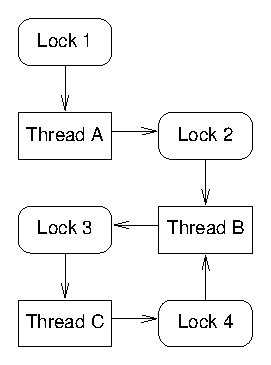
\includegraphics{locking/DeadlockCycle}}
\end{center}
\caption{Deadlock Cycle}
\label{fig:locking:Deadlock Cycle}
\end{figure}

We can create a directed-graph representation of a deadlock scenario
with nodes for threads and locks, as shown in
Figure~\ref{fig:locking:Deadlock Cycle}.
An arrow from a lock to a thread indicates that the thread holds
the lock, for example, Thread~B holds Locks~2 and 4.
An arrow from a thread to a lock indicates that the thread is waiting
on the lock, for example, Thread~B is waiting on Lock~3.

A deadlock scenario will always contain at least one deadlock cycle.
In Figure~\ref{fig:locking:Deadlock Cycle}, this cycle is
Thread~B, Lock~3, Thread~C, Lock~4, and back to Thread~B.

\QuickQuiz{}
	But the definition of deadlock only said that each thread
	was holding at least one lock and waiting on another lock
	that was held by some thread.
	How do you know that there is a cycle?
\QuickQuizAnswer{
	Suppose that there is no cycle in the graph.
	We would then have a directed acyclic graph (DAG), which would
	have at least one leaf node.

	If this leaf node was a lock, then we would have a thread
	that was waiting on a lock that wasn't held by any thread,
	which violates the definition.
	(And in this case the thread would immediately acquire the
	lock.)

	On the other hand, if this leaf node was a thread, then
	we would have a thread that was not waiting on any lock,
	again violating the definition.
	(And in this case, the thread would either be running or
	be blocked on something that is not a lock.)

	Therefore, given this definition of deadlock, there must
	be a cycle in the corresponding graph.
} \QuickQuizEnd

Although there are some software environments such as database systems
that can repair an existing deadlock, this approach requires either that
one of the threads be killed or that a lock be forcibly stolen from one
of the threads.
This killing and forcible stealing can be appropriate for transactions,
but is often problematic for kernel and application-level use of locking:
dealing with the resulting partially updated structures can be extremely
complex, hazardous, and error-prone.

Kernels and applications therefore work to avoid deadlocks rather than to
recover from them.
There are a number of deadlock-avoidance strategies,
including locking hierarchies
(Section~\ref{sec:locking:Locking Hierarchies}),
local locking hierarchies
(Section~\ref{sec:locking:Local Locking Hierarchies}),
layered locking hierarchies
(Section~\ref{sec:locking:Layered Locking Hierarchies}),
strategies for dealing with APIs containing pointers to locks
(Section~\ref{sec:locking:Locking Hierarchies and Pointers to Locks}),
conditional locking
(Section~\ref{sec:locking:Conditional Locking}),
acquiring all needed locks first
(Section~\ref{sec:locking:Acquire Needed Locks First}),
single-lock-at-a-time designs
(Section~\ref{sec:locking:Single-Lock-at-a-Time Designs}),
and strategies for signal/interrupt handlers
(Section~\ref{sec:locking:Signal/Interrupt Handlers}).
Although there is no deadlock-avoidance strategy that works perfectly
for all situations, there is a good selection of deadlock-avoidance
tools to choose from.

\subsubsection{Locking Hierarchies}
\label{sec:locking:Locking Hierarchies}

Locking hierarchies order the locks and prohibit acquiring locks out
of order.
In Figure~\ref{fig:locking:Deadlock Cycle},
we might order the locks numerically, so that a thread was
forbidden from acquiring a given lock if it already held a lock
with the same or a higher number.
Thread~B has violated this hierarchy because it is attempting to
acquire Lock~3 while holding Lock~4, which permitted the deadlock
to occur.

Again, to apply a locking hierarchy, order the locks and prohibit
out-of-order lock acquisition.
In large program, it is wise to use tools to enforce your locking
hierarchy~\cite{JonathanCorbet2006lockdep}.

\subsubsection{Local Locking Hierarchies}
\label{sec:locking:Local Locking Hierarchies}

However, the global nature of locking hierarchies make them difficult to
apply to library functions.
After all, the program using a given library function has not even been
written yet, so how can the poor library-function implementor possibly
hope to adhere to the yet-to-be-written program's locking hierarchy?

One special case that is fortunately the common case is when
the library function does not invoke any of the caller's code.
In this case, the caller's locks will never be acquired while holding
any of the library's locks, so that there cannot be a deadlock cycle
containing locks from both the library and the caller.

\QuickQuiz{}
	Are there any exceptions to this rule, so that there really could be
	a deadlock cycle containing locks from both the library and
	the caller, even given that the library code never invokes
	any of the caller's functions?
\QuickQuizAnswer{
	Indeed there are!
	Here are a few of them:
	\begin{enumerate}
	\item	If one of the library function's arguments is a pointer
		to a lock that this library function acquires, and if
		the library function holds one if its locks while
		acquiring the caller's lock, then we could have a
		deadlock cycle involving both caller and library locks.
	\item	If one of the library functions returns a pointer to
		a lock that is acquired by the caller, and if the
		caller acquires one if its locks while holding the
		library's lock, we could again have a deadlock
		cycle involving both caller and library locks.
	\item	If one of the library functions acquires a lock and
		then returns while still holding it, and if the caller
		acquires one of its locks, we have yet another way
		to create a deadlock cycle involving both caller
		and library locks.
	\item	If the caller has a signal handler that acquires
		locks, then the deadlock cycle can involve both
		caller and library locks.
		In this case, however, the library's locks are
		innocent bystanders in the deadlock cycle.
		That said, please note that acquiring a lock from
		within a signal handler is a no-no in most
		environments---it is not just a bad idea, it
		is unsupported.
	\end{enumerate}
} \QuickQuizEnd

But suppose that a library function does invoke the caller's code.
For example, the \co{qsort()} function invokes a caller-provided
comparison function.
A concurrent implementation of \co{qsort()} likely uses locking,
which might result in deadlock in the perhaps-unlikely case where
the comparison function is a
complicated function involving also locking.
How can the library function avoid deadlock?

The golden rule in this case is ``release all locks before invoking
unknown code.''
To follow this rule, the \co{qsort()} function must release all
locks before invoking the comparison function.

\QuickQuiz{}
	But if \co{qsort()} releases all its locks before invoking
	the comparison function, how can it protect against races
	with other \co{qsort()} threads?
\QuickQuizAnswer{
	By privatizing the data elements being compared
	(as discussed in Chapter~\ref{chp:Data Ownership})
	or through use of deferral mechanisms such as
	reference counting (as discussed in
	Chapter~\ref{chp:Deferred Processing}).
} \QuickQuizEnd

\begin{figure}[tb]
\begin{center}
\resizebox{3in}{!}{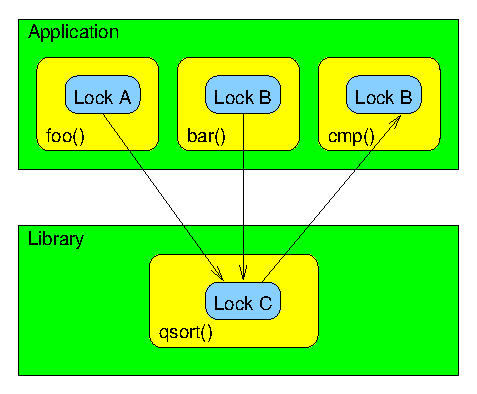
\includegraphics{locking/NonLocalLockHierarchy}}
\end{center}
\caption{Without Local Locking Hierarchy for qsort()}
\label{fig:lock:Without Local Locking Hierarchy for qsort()}
\end{figure}

\begin{figure}[tb]
\begin{center}
\resizebox{3in}{!}{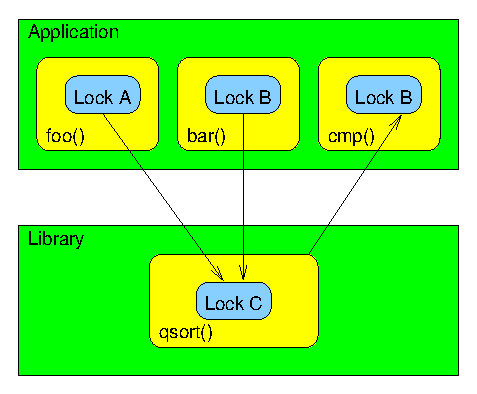
\includegraphics{locking/LocalLockHierarchy}}
\end{center}
\caption{Local Locking Hierarchy for qsort()}
\label{fig:lock:Local Locking Hierarchy for qsort()}
\end{figure}

To see the benefits of local locking hierarchies, compare
Figures~\ref{fig:lock:Without Local Locking Hierarchy for qsort()} and
\ref{fig:lock:Local Locking Hierarchy for qsort()}.
In both figures, application functions \co{foo()} and \co{bar()}
invoke \co{qsort()} while holding locks~A and B, respectively.
Because this is a parallel implementation of \co{qsort()}, it acquires
lock~C.
Function \co{foo()} passes function \co{cmp()} to \co{qsort()},
and \co{cmp()} acquires lock~B.
Function \co{bar()} passes a simple integer-comparison function (not
shown) to \co{qsort()}, and this simple function does not acquire any
locks.

Now, if \co{qsort()} holds Lock~C while calling \co{cmp()} in violation
of the golden release-all-locks rule above, as shown in
Figure~\ref{fig:lock:Without Local Locking Hierarchy for qsort()},
deadlock can occur.
To see this, suppose that one thread invokes \co{foo()} while a second
thread concurrently invokes \co{bar()}.
The first thread will acquire lock~A and the second thread will acquire
lock~B.
If the first thread's call to \co{qsort()} acquires lock~C, then it
will be unable to acquire lock~B when it calls \co{cmp()}.
But the first thread holds lock~C, so the second thread's call to
\co{qsort()} will be unable to acquire it, and thus unable to release
lock~B, resulting in deadlock.

In contrast, if \co{qsort()} releases lock~C before invoking the
comparison function (which is unknown code from \co{qsort()}'s perspective,
then deadlock is avoided as shown in
Figure~\ref{fig:lock:Local Locking Hierarchy for qsort()}.

If each module releases all locks before invoking unknown code, then
deadlock is avoided if each module separately avoids deadlock.
This rule therefore greatly simplifies deadlock analysis and greatly
improves modularity.

\subsubsection{Layered Locking Hierarchies}
\label{sec:locking:Layered Locking Hierarchies}

\begin{figure}[tb]
\begin{center}
\resizebox{3in}{!}{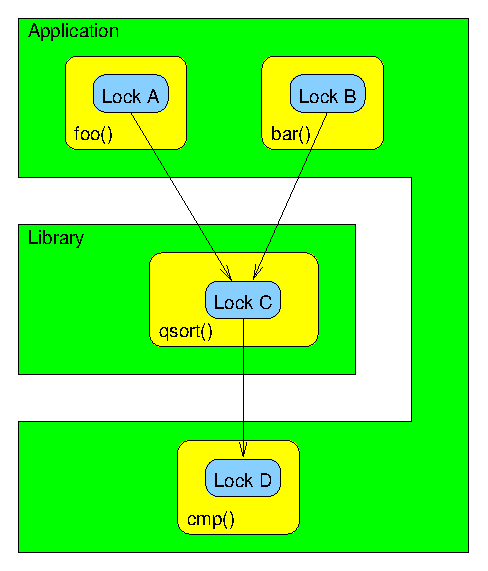
\includegraphics{locking/LayeredLockHierarchy}}
\end{center}
\caption{Layered Locking Hierarchy for qsort()}
\label{fig:lock:Layered Locking Hierarchy for qsort()}
\end{figure}

Unfortunately, it might not be possible for \co{qsort()} to release
all of its locks before invoking the comparison function.
In this case, we cannot construct a local locking hierarchy by
releasing all locks before invoking unknown code.
However, we can instead construct a layered locking hierarchy, as shown in
Figure~\ref{fig:lock:Layered Locking Hierarchy for qsort()}.
Here, the \co{cmp()} function uses a new lock~D that is acquired after
all of locks~A, B, and C, avoiding deadlock.
We therefore have three layers to the global deadlock hierarchy, the
first containing locks~A and B, the second containing lock~C, and
the third containing lock~D.

\begin{figure}[tbp]
{ \scriptsize
\begin{verbatim}
  1 struct locked_list {
  2   spinlock_t s;
  3   struct list_head h;
  4 };
  5 
  6 struct list_head *list_start(struct locked_list *lp)
  7 {
  8   spin_lock(&lp->s);
  9   return list_next(lp, &lp->h);
 10 }
 11 
 12 struct list_head *list_next(struct locked_list *lp,
 13                             struct list_head *np)
 14 {
 15   struct list_head *ret;
 16 
 17   ret = np->next;
 18   if (ret == &lp->h) {
 19     spin_unlock(&lp->s);
 20     ret = NULL;
 21   }
 22   return ret;
 23 }
\end{verbatim}
}
\caption{Concurrent List Iterator}
\label{fig:locking:Concurrent List Iterator}
\end{figure}

Please note that it is not typically possible to mechanically
change \co{cmp()} to use the new Lock~D.
Quite the opposite: It is often necessary to make profound design-level
modifications.
Nevertheless, the effort required for such modifications is normally
a small price to pay in order to avoid deadlock.

For another example where releasing all locks before invoking unknown
code is impractical, imagine an iterator over a linked list, as shown in
Figure~\ref{fig:locking:Concurrent List Iterator} (\co{locked_list.c}).
The \co{list_start()} function acquires a lock on the list and returns
the first element (if there is one), and
\co{list_next()} either returns a pointer to the next element in the list
or releases the lock and returns \co{NULL} if the end of the list has
been reached.

\begin{figure}[tbp]
{ \scriptsize
\begin{verbatim}
  1 struct list_ints {
  2   struct list_head n;
  3   int a;
  4 };
  5 
  6 void list_print(struct locked_list *lp)
  7 {
  8   struct list_head *np;
  9   struct list_ints *ip;
 10 
 11   np = list_start(lp);
 12   while (np != NULL) {
 13     ip = list_entry(np, struct list_ints, n);
 14     printf("\t%d\n", ip->a);
 15     np = list_next(lp, np);
 16   }
 17 }
\end{verbatim}
}
\caption{Concurrent List Iterator Usage}
\label{fig:locking:Concurrent List Iterator Usage}
\end{figure}

Figure~\ref{fig:locking:Concurrent List Iterator Usage} shows how
this list iterator may be used.
Lines~1-4 define the \co{list_ints} element containing a single integer,
and lines~6-17 show how to iterate over the list.
Line~11 locks the list and fetches a pointer to the first element,
line~13 provides a pointer to our enclosing \co{list_ints} structure,
line~14 prints the corresponding integer, and
line~15 moves to the next element.
This is quite simple, and hides all of the locking.

That is, the locking remains hidden as long as the code processing each
list element does not itself acquire a lock that is held across some
other call to \co{list_start()} or \co{list_next()}, which results in
deadlock.
We can avoid the deadlock by layering the locking hierarchy
to take the list-iterator locking into account.

This layered approach can be extended to an arbitrarily large number of layers,
but each added layer increases the complexity of the locking design.
Such increases in complexity are particularly inconvenient for some
types of object-oriented designs, in which control passes back and forth
among a large group of objects in an undisciplined manner.\footnote{
	One name for this is ``object-oriented spaghetti code.''}
This mismatch between the habits of object-oriented design and the
need to avoid deadlock is an important reason why parallel programming
is perceived by some to be so difficult.

Some alternatives to highly layered locking hierarchies are covered in
Chapter~\ref{chp:Deferred Processing}.

\subsubsection{Locking Hierarchies and Pointers to Locks}
\label{sec:locking:Locking Hierarchies and Pointers to Locks}

Althought there are some exceptions, an external API containing a pointer
to a lock is very often a misdesigned API.
Handing an internal lock to some other software component is after all
the antithesis of information hiding, which is in turn a key design
principle.

\QuickQuiz{}
	Name one common exception where it is perfectly reasonable
	to pass a pointer to a lock into a function.
\QuickQuizAnswer{
	Locking primitives, of course!
} \QuickQuizEnd

One exception is functions that hand off some entity,
where the caller's lock must be held until the handoff is complete,
but where the lock must be released before the function returns.
One example of such a function is the POSIX \co{pthread_cond_wait()}
function, where passing an pointer to a \co{pthread_mutex_t}
prevents hangs due to lost wakeups.

\QuickQuiz{}
	Doesn't the fact that \co{pthread_cond_wait()} first releases the
	mutex and then re-acquires it eliminate the possibility of deadlock?
\QuickQuizAnswer{
	Absolutely not!

	Consider the a program that acquires \co{mutex_a}, and then
	\co{mutex_b}, in that order, and then passes \co{mutex_a}
	to \co{pthread_cond_wait}.
	Now, \co{pthread_cond_wait} will release \co{mutex_a}, but
	will re-acquire it before returning.
	If some other thread acquires \co{mutex_a} in the meantime
	and then blocks on \co{mutex_b}, the program will deadlock.
} \QuickQuizEnd

In short, if you find yourself exporting an API with a pointer to a
lock as an argument or the return value, do youself a favor and carefully
reconsider your API design.
It might well be the right thing to do, but experience indicates that
this is unlikely.

\subsubsection{Conditional Locking}
\label{sec:locking:Conditional Locking}

\begin{figure}[tbp]
{ \scriptsize
\begin{verbatim}
  1 spin_lock(&lock2);
  2 layer_2_processing(pkt);
  3 nextlayer = layer_1(pkt);
  4 spin_lock(&nextlayer->lock1);
  5 layer_1_processing(pkt);
  6 spin_unlock(&lock2);
  7 spin_unlock(&nextlayer->lock1);
\end{verbatim}
}
\caption{Protocol Layering and Deadlock}
\label{fig:locking:Protocol Layering and Deadlock}
\end{figure}

But suppose that there is no reasonable locking hierarchy.
This can happen in real life, for example, in layered network protocol stacks
where packets flow in both directions.
In the networking case, it might be necessary to hold the locks from
both layers when passing a packet from one layer to another.
Given that packets travel both up and down the protocol stack, this
is an excellent recipe for deadlock, as illustrated in
Figure~\ref{fig:locking:Protocol Layering and Deadlock}.
Here, a packet moving down the stack towards the wire must acquire
the next layer's lock out of order.
Given that packets moving up the stack away from the wire are acquiring
the locks in order, the lock acquisition in line~4 of the figure
can result in deadlock.

\begin{figure}[tbp]
{ \scriptsize
\begin{verbatim}
  1 retry:
  2   spin_lock(&lock2);
  3   layer_2_processing(pkt);
  4   nextlayer = layer_1(pkt);
  5   if (!spin_trylock(&nextlayer->lock1)) {
  6     spin_unlock(&lock2);
  7     spin_lock(&nextlayer->lock1);
  8     spin_lock((&lock2);
  9     if (layer_1(pkt) != nextlayer) {
 10       spin_unlock(&nextlayer->lock1);
 11       spin_unlock((&lock2);
 12       goto retry;
 13     }
 14   }
 15   layer_1_processing(pkt);
 16 spin_unlock(&lock2);
 17 spin_unlock(&nextlayer->lock1);
\end{verbatim}
}
\caption{Avoiding Deadlock Via Conditional Locking}
\label{fig:locking:Avoiding Deadlock Via Conditional Locking}
\end{figure}

One way to avoid deadlocks in this case is to impose a locking hierarchy,
but when it is necessary to acquire a lock out of order, acquire it
conditionally, as shown in
Figure~\ref{fig:locking:Avoiding Deadlock Via Conditional Locking}.
Instead of unconditionally acquiring the layer-1 lock, line~5
conditionally acquires the lock using the \co{spin_trylock()} primitive.
This primitive acquires the lock immediately if the lock is available
(returning non-zero), and otherwise returns zero without acquiring the lock.

If \co{spin_trylock()} was successful, line~15 does the needed
layer-1 processing.
Otherwise, line~6 releases the lock, and lines~7 and 8 acquire them in
the correct order.
Unfortunately, there might be multiple networking devices on
the system (e.g., Ethernet and WiFi), so that the \co{layer_1()}
function must make a routing decision.
This decision might change at any time, especially if the system
is mobile.\footnote{
	And, in contrast to the 1900s, mobility is the common case.}
Therefore, line~9 must recheck the decision, and if it has changed,
must release the locks and start over.

\QuickQuiz{}
	Can the transformation from
	Figure~\ref{fig:locking:Protocol Layering and Deadlock} to
	Figure~\ref{fig:locking:Avoiding Deadlock Via Conditional Locking}
	be applied universally?
\QuickQuizAnswer{
	Absolutely not!

	This transformation assumes that the
	\co{layer_2_processing()} function is idempotent, given that
	it might be executed multiple times on the same packet when
	the \co{layer_1()} routing decision changes.
	Therefore, in real life, this transformation can become
	arbitrarily complex.
} \QuickQuizEnd

\QuickQuiz{}
	But the complexity in
	Figure~\ref{fig:locking:Avoiding Deadlock Via Conditional Locking}
	is well worthwhile given that it avoids deadlock, right?
\QuickQuizAnswer{
	Maybe.

	If the routing decision in \co{layer_1()} changes often enough,
	the code will always retry, never making forward progress.
	This is termed ``livelock'' if no thread makes any forward progress or
	``starvation''
	if some threads make forward progress but other do not
	(see Section~\ref{sec:locking:Livelock and Starvation}).
} \QuickQuizEnd

\subsubsection{Acquire Needed Locks First}
\label{sec:locking:Acquire Needed Locks First}

In an important special case of conditional locking all needed
locks are acquired before any processing is carried out.
In this case, processing need not be idempotent: if it turns out
to be impossible to acquire a given lock without first releasing
one that was already acquired, just release all the locks and
try again.
Only once all needed locks are held will any processing be carried out.

However, this procedure can result in \emph{livelock}, which will
be discussed in
Section~\ref{sec:locking:Livelock and Starvation}.

\QuickQuiz{}
	When using the ``acquire needed locks first'' approach described in
	Section~\ref{sec:locking:Acquire Needed Locks First},
	how can livelock be avoided?
\QuickQuizAnswer{
	Provide an additional global lock.
	If a given thread has repeatedly tried and failed to acquire the needed
	locks, then have that thread unconditionally acquire the new
	global lock, and then unconditionally acquire any needed locks.
	(Suggested by Doug Lea.)
} \QuickQuizEnd

A related approach, two-phase locking~\cite{PhilipABernstein1987},
has seen long production use in database systems.
Many such systems rely on the ability to abort transactions, although
this can be simplified by avoiding making any changes to shared data
until all needed locks are acquired.
Livelock and deadlock are issues in such systems, but practical
solutions may be found in any of a number of database textbooks.

\subsubsection{Single-Lock-at-a-Time Designs}
\label{sec:locking:Single-Lock-at-a-Time Designs}

In some cases, it is possible to avoid nesting locks, thus avoiding
deadlock.
For example, if a problem is perfectly partitionable, a single
lock may be assigned to each partition.
Then a thread working on a given partition need only acquire the one
corresponding lock.
Because no thread ever holds more than one lock at a time,
deadlock is impossible.

However, there must be some mechanism to ensure that the needed data
structures remain in existence during the time that neither lock is
held.
One such mechanism is discussed in
Section~\ref{sec:locking:Lock-Based Existence Guarantees}
and several others are presented in
Chapter~\ref{chp:Deferred Processing}.

\subsubsection{Signal/Interrupt Handlers}
\label{sec:locking:Signal/Interrupt Handlers}

Deadlocks involving signal handlers are often quickly dismissed by
noting that it is not legal to invoke \co{pthread_mutex_lock()} from
within a signal handler~\cite{OpenGroup1997pthreads}.
However, it is possible (though almost always unwise) to hand-craft
locking primitives that can be invoked from signal handlers.
Besides which, almost all operating-system kernels permit locks to
be acquired from within interrupt handlers, which are the kernel analog
to signal handlers.

The trick is to block signals (or disable interrupts, as the case may be)
when acquiring any lock that might be acquired within an interrupt
handler.
Furthermore, if holding such a lock, it is illegal to attempt to
acquire any lock that is ever acquired
outside of a signal handler without blocking signals.

\QuickQuiz{}
	Why is it illegal to acquire a Lock~A that is acquired outside
	of a signal handler without blocking signals while holding
	a Lock~B that is acquired within a signal handler?
\QuickQuizAnswer{
	Because this would lead to deadlock.
	Given that Lock~A is held outside of a signal
	handler without blocking signals, a signal might be handled while
	holding this lock.
	The corresponding signal handler might then acquire
	Lock~B, so that Lock~B is acquired while holding Lock~A.
	Therefore, if we also acquire Lock~A while holding Lock~B
	as called out in the question, we will have a deadlock cycle.

	Therefore, it is illegal to acquire a lock that is acquired outside
	of a signal handler without blocking signals while holding
	a another lock that is acquired within a signal handler.
} \QuickQuizEnd

If a lock is acquired by the handlers for several signals, then each
and every one of these signals must be blocked whenever that lock is
acquired, even when that
lock is acquired within a signal handler.

\QuickQuiz{}
	How can you legally block signals within a signal handler?
\QuickQuizAnswer{
	One of the simplest and fastest ways to do so is to use
	the \co{sa_mask} field of the \co{struct sigaction} that
	you pass to \co{sigaction()} when setting up the signal.
} \QuickQuizEnd

Unfortunately, blocking and unblocking signals can be expensive in
some operating systems, notably including Linux, so performance
concerns often mean that locks acquired in signal handlers are only
acquired in signal handlers, and that lockless synchronization
mechanisms are used to communicate between application code and
signal handlers.

Or that signal handlers are avoided completely except for handling
fatal errors.

\QuickQuiz{}
	If acquiring locks in signal handlers is such a bad idea, why
	even discuss ways of making it safe?
\QuickQuizAnswer{
	Because these same rules apply to the interrupt handlers used in
	operating-system kernels and in some embedded applications.

	In many application environments, acquiring locks in signal
	handlers is frowned upon~\cite{OpenGroup1997pthreads}.
	However, that does not stop clever developers from (usually
	unwisely) fashioning home-brew locks out of atomic operations.
	And atomic operations are in many cases perfectly legal in
	signal handlers.
} \QuickQuizEnd

\subsubsection{Discussion}
\label{sec:locking:Locking Hierarchy Discussion}

There are a large number of deadlock-avoidance strategies available to
the shared-memory parallel programmer, but there are sequential
programs for which none of them is a good fit.
This is one of the reasons that expert programmers have more than
one tool in their toolbox: locking is a powerful concurrency
tool, but there are jobs better addressed with other tools.

\QuickQuiz{}
	Given an object-oriented application that passes control freely
	among a group of objects such that there is no straightforward
	locking hierarchy,\footnote{
		Also known as ``object-oriented spaghetti code.''}
	layered or otherwise, how can this
	application be parallelized?
\QuickQuizAnswer{
	There are a number of approaches:
	\begin{enumerate}
	\item	In the case of parametric search via simulation,
		where a large number of simulations will be run
		in order to converge on (for example) a good design
		for a mechanical or electrical device, leave the
		simulation single-threaded, but run many instances
		of the simulation in parallel.
		This retains the object-oriented design, and
		gains parallelism at a higher level, and likely
		also avoids synchronization overhead.
	\item	Partition the objects into groups such that there
		is no need to operate on objects in
		more than one group at a given time.
		Then associate a lock with each group.
		This is an example of a single-lock-at-a-time
		design, which discussed in
		Section~\ref{sec:locking:Single-Lock-at-a-Time Designs}.
	\item	Partition the objects into groups such that threads
		can all operate on objects in the groups in some
		groupwise ordering.
		Then associate a lock with each group, and impose a
		locking hierarchy over the groups.
	\item	Impose an arbitrarily selected hierarchy on the locks,
		and then use conditional locking if it is necessary
		to acquire a lock out of order, as was discussed in
		Section~\ref{sec:locking:Conditional Locking}.
	\item	Before carrying out a given group of operations, predict
		which locks will be acquired, and attempt to acquire them
		before actually carrying out any updates.
		If the prediction turns out to be incorrect, drop
		all the locks and retry with an updated prediction
		that includes the benefit of experience.
		This approach was discussed in
		Section~\ref{sec:locking:Acquire Needed Locks First}.
	\item	Use transactional memory.
		This approach has a number of advantages and disadvantages
		which will be discussed in
		Section~\ref{sec:future:Transactional Memory}.
	\item	Refactor the application to be more concurrency-friendly.
		This would likely also have the side effect of making
		the application run faster even when single-threaded, but might
		also make it more difficult to modify the application.
	\item	Use techniques from later chapters in addition to locking.
	\end{enumerate}
} \QuickQuizEnd

Nevertheless, the strategies described in this section have proven
quite useful in many settings.

\subsection{Livelock and Starvation}
\label{sec:locking:Livelock and Starvation}

\begin{figure}[tbp]
{ \scriptsize
\begin{verbatim}
  1 void thread1(void)
  2 {
  3 retry:
  4   spin_lock(&lock1);
  5   do_one_thing();
  6   if (!spin_trylock(&lock2)) {
  7     spin_unlock(&lock1);
  8     goto retry;
  9   }
 10   do_another_thing();
 11   spin_unlock(&lock2);
 12   spin_unlock(&lock1);
 13 }
 14 
 15 void thread2(void)
 16 {
 17 retry:
 18   spin_lock(&lock2);
 19   do_a_third_thing();
 20   if (!spin_trylock(&lock1)) {
 21     spin_unlock(&lock2);
 22     goto retry;
 23   }
 24   do_a_fourth_thing();
 25   spin_unlock(&lock1);
 26   spin_unlock(&lock2);
 27 }
\end{verbatim}
}
\caption{Abusing Conditional Locking}
\label{fig:locking:Abusing Conditional Locking}
\end{figure}

Although conditional locking can be an effective deadlock-avoidance
mechanism, it can be abused.
Consider for example the beautifully symmetric example shown in
Figure~\ref{fig:locking:Abusing Conditional Locking}.
This example's beauty hides an ugly livelock.
To see this, consider the following sequence of events:

\begin{enumerate}
\item	Thread~1 acquires \co{lock1} on line~4, then invokes
	\co{do_one_thing()}.
\item	Thread~2 acquires \co{lock2} on line~18, then invokes
	\co{do_a_third_thing()}.
\item	Thread~1 attempts to acquire \co{lock2} on line~6, but fails because
	Thread~2 holds it.
\item	Thread~2 attempts to acquire \co{lock1} on line~20, but fails because
	Thread~1 holds it.
\item	Thread~1 releases \co{lock1} on line~7, then jumps to \co{retry}
	at line~3.
\item	Thread~2 releases \co{lock2} on line~21, and jumps to \co{retry}
	at line~17.
\item	The livelock dance repeats from the beginning.
\end{enumerate}

\QuickQuiz{}
	How can the livelock shown in
	Figure~\ref{fig:locking:Abusing Conditional Locking}
	be avoided?
\QuickQuizAnswer{
	Figure~\ref{fig:locking:Avoiding Deadlock Via Conditional Locking}
	provides some good hints.
	In many cases, livelocks are a hint that you should revisit your
	locking design.
	Or visit it in the first place if your locking design
	``just grew''.

	That said, one good-and-sufficient approach due to Doug Lea
	is to use conditional locking as described in
	Section~\ref{sec:locking:Conditional Locking}, but combine this
	with acquiring all needed locks first, before modifying shared
	data, as described in
	Section~\ref{sec:locking:Acquire Needed Locks First}.
	If a given critical section retries too many times,
	unconditionally acquire
	a global lock, then unconditionally acquire all the needed locks.
	This avoids both deadlock and livelock, and scales reasonably
	assuming that the global lock need not be acquired too often.
} \QuickQuizEnd

Starvation is very similar to livelock.
Put another way, livelock is an extreme form of starvation where
a group of threads starve, rather than just one of them.\footnote{
	Try not to get too hung up on the exact definitions of terms
	like livelock, starvation, and unfairness.
	Anything that causes a group of threads to fail to make adequate
	forward progress is a problem that needs to be fixed, regardless
	of what name you choose for it.}

\begin{figure}[tbp]
{ \scriptsize
\begin{verbatim}
  1 void thread1(void)
  2 {
  3   unsigned int wait = 1;
  4 retry:
  5   spin_lock(&lock1);
  6   do_one_thing();
  7   if (!spin_trylock(&lock2)) {
  8     spin_unlock(&lock1);
  9     sleep(wait);
 10     wait = wait << 1;
 11     goto retry;
 12   }
 13   do_another_thing();
 14   spin_unlock(&lock2);
 15   spin_unlock(&lock1);
 16 }
 17 
 18 void thread2(void)
 19 {
 20   unsigned int wait = 1;
 21 retry:
 22   spin_lock(&lock2);
 23   do_a_third_thing();
 24   if (!spin_trylock(&lock1)) {
 25     spin_unlock(&lock2);
 26     sleep(wait);
 27     wait = wait << 1;
 28     goto retry;
 29   }
 30   do_a_fourth_thing();
 31   spin_unlock(&lock1);
 32   spin_unlock(&lock2);
 33 }
\end{verbatim}
}
\caption{Conditional Locking and Exponential Backoff}
\label{fig:locking:Conditional Locking and Exponential Backoff}
\end{figure}

Livelock and starvation are serious issues in software transactional
memory implementations, and so the concept of \emph{contention
manager} has been introduced to encapsulate these issues.
In the case of locking, simple exponential backoff can often address
livelock and starvationh.
The idea is to introduce exponentially increasing delays before each
retry, as shown in
Figure~\ref{fig:locking:Conditional Locking and Exponential Backoff}.

\QuickQuiz{}
	What problems can you spot in the code in
	Figure~\ref{fig:locking:Conditional Locking and Exponential Backoff}?
\QuickQuizAnswer{
	Here are a couple:
	\begin{enumerate}
	\item	A one-second wait is way too long for most uses.
		Wait intervals should begin with roughly the time
		required to execute the critical section, which will
		normally be in the microsecond or millisecond range.
	\item	The code does not check for overflow.
		On the other hand, this bug is nullified 
		by the previous bug: 32 bits worth of seconds is
		more than 50 years.
	\end{enumerate}
} \QuickQuizEnd

However, for better results, the backoff should be bounded, and
even better high-contention results have been obtained via queued
locking~\cite{Anderson90}, which is discussed more in
Section~\ref{sec:locking:Other Exclusive-Locking Implementations}.
Of course, best of all is to use a good parallel design so that lock
contention remains low.

\subsection{Unfairness}
\label{sec:locking:Unfairness}

\begin{figure}[tb]
\begin{center}
\resizebox{3in}{!}{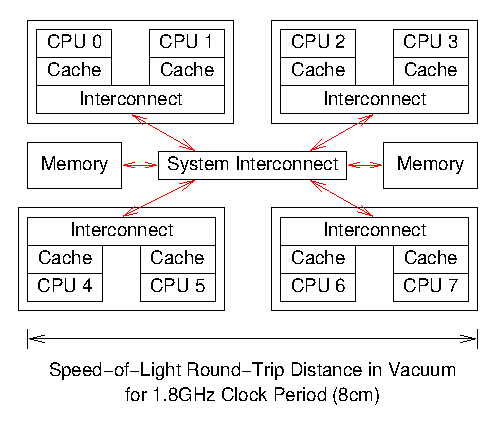
\includegraphics{cpu/SystemArch}}
\end{center}
\caption{System Architecture and Lock Unfairness}
\label{fig:lock:System Architecture and Lock Unfairness}
\end{figure}

Unfairness can be thought of as a less-severe form of starvation,
where a subset of threads contending for a given lock are granted
the lion's share of the acquisitions.
This can happen on machines with shared caches or NUMA characteristics,
for example, as shown in
Figure~\ref{fig:lock:System Architecture and Lock Unfairness}.
If CPU~0 releases a lock that all the other CPUs are attempting
to acquire, the interconnect shared between CPUs~0 and 1 means that
CPU~1 will have an advantage over CPUs~2-7.
Therefore CPU~1 will likely acquire the lock.
If CPU~1 hold the lock long enough for CPU~0 to be requesting the
lock by the time CPU~1 releases it and vice versa, the lock can
shuttle between CPUs~0 and 1, bypassing CPUs~2-7.

\QuickQuiz{}
	Wouldn't it be better just to use a good parallel design
	so that lock contention was low enough to avoid unfairness?
\QuickQuizAnswer{
	It would be better in some sense, but there are situations
	where it can be appropriate to use
	designs that sometimes result in high lock contentions.

	For example, imagine a system that is subject to a rare error
	condition.
	It might well be best to have a simple error-handling design
	that has poor performance and scalability for the duration of
	the rare error condition, as opposed to a complex and
	difficult-to-debug design that is helpful only when one of
	those rare error conditions is in effect.

	That said, it is usually worth putting some effort into
	attempting to produce a design that both simple as well as
	efficient during error conditions, for example by partitioning
	the problem.
} \QuickQuizEnd

\subsection{Inefficiency}
\label{sec:locking:Inefficiency}

Locks are implemented using atomic instructions and memory barriers,
and often involve cache misses.
As we saw in Chapter~\ref{chp:Hardware and its Habits},
these instructions are quite expensive, roughly two
orders of magnitude greater overhead than simple instructions.
This can be a serious problem for locking: If you protect a single
instruction with a lock, you will increase the overhead by a factor
of one hundred.
Even assuming perfect scalability, \emph{one hundred} CPUs would
be required to keep up with a single CPU executing the same code
without locking.

This situation underscores the synchronization-granularity
tradeoff discussed in Section~\ref{sec:SMPdesign:Synchronization Granularity},
especially Figure~\ref{fig:SMPdesign:Synchronization Efficiency}:
Too coarse a granularity will limit scalability, while too fine a
granularity will result in excessive synchronization overhead.

That said, once a lock is held, the data protected by that lock can
be accessed by the lock holder without interference.
Acquiring a lock might be expensive, but once held, the CPU's caches
are an effective performance booster, at least for large critical sections.

\QuickQuiz{}
	How might the lock holder be interfered with?
\QuickQuizAnswer{
	If the data protected by the lock is in the same cache line
	as the lock itself, then attempts by other CPUs to acquire
	the lock will result in expensive cache misses on the part
	of the CPU holding the lock.
	This is a special case of false sharing, which can also occur
	if a pair of variables protected by different locks happen
	to share a cache line.
	In contrast, if the lock is in a different cache line than
	the data that it protects, the CPU holding the lock will
	usually suffer a cache miss only on first access to a given
	variable.

	Of course, the downside of placing the lock and data into separate
	cache lines is that the code will incur two cache misses rather
	than only one in the uncontended case.
} \QuickQuizEnd

\section{Types of Locks}
\label{sec:locking:Types of Locks}

There are a surprising number of types of locks, more than this
short chapter can possibly do justice to.
The following sections discuss
exclusive locks (Section~\ref{sec:locking:Exclusive Locks}),
reader-writer locks (Section~\ref{sec:locking:Reader-Writer Locks}),
multi-role locks (Section~\ref{sec:locking:Beyond Reader-Writer Locks}),
and scoped locking (Section~\ref{sec:locking:Scoped Locking}).

\subsection{Exclusive Locks}
\label{sec:locking:Exclusive Locks}

Exclusive locks are what they say they are: only one thread may hold
the lock at a time.
The holder of such a lock thus has exclusive access to all data protected
by that lock, hence the name.

Of course, this all assumes that this lock is held across all accesses
to data purportedly protected by the lock.
Although there are some tools that can help, the ultimate responsibility
for ensuring that the lock is acquired in all necessary code paths
rests with the developer.

\QuickQuiz{}
	Does it ever make sense to have an exclusive lock acquisition
	immediately followed by a release of that same lock, that is,
	an empty critical section?
\QuickQuizAnswer{
	This usage is rare, but is occasionally used.
	The point is that the semantics of exclusive locks have two
	components: (1)~the familiar data-protection semantic and
	(2)~a messaging semantic, where releasing a given lock notifies
	a waiting acquisition of that same lock.

	One historical use of empty critical sections appeared in the
	networking stack of the 2.4 Linux kernel.
	This usage pattern can be thought of as a way of approximating
	the effects of read-copy update (RCU), which is discussed in
	Section~\ref{sec:defer:Read-Copy Update (RCU)}.

	The empty-lock-critical-section idiom can also be used to
	reduce lock contention in some situations.
	For example, consider a multithreaded user-space application where
	each thread processes unit of work maintained in a per-thread
	list, where thread are prohibited from touching each others'
	lists.
	There could also be updates that require that all previously
	scheduled units of work have completed before the update can
	progress.
	One way to handle this is to schedule a unit of work on each
	thread, so that when all of these units of work complete, the
	update may proceed.

	In some applications, threads can come and go.
	For example, each thread might correspond to one user of the
	application, and thus be removed when that user logs out or
	otherwise disconnects.
	In many applications, threads cannot depart atomically: They must
	instead explicitly unravel themselves from various portions of
	the application using a specific sequence of actions.
	One specific action will be refusing to accept further requests
	from other threads, and another specific action will be disposing
	of any remaining units of work on its list, for example, by
	placing these units of work in a global work-item-disposal list
	to be taken by one of the remaining threads.
	(Why not just drain the thread's work-item list by executing
	each item?
	Because a given work item might generate more work items, so
	that the list could not be drained in a timely fashion.)

	If the application is to perform and scale well, a good locking
	design is required.
	One common solution is to have a global lock (call it \co{G})
	protecting the entire
	process of departing (and perhaps other things as well),
	with finer-grained locks protecting the
	individual unraveling operations.

	Now, a departing thread must clearly refuse to accept further
	requests before disposing of the work on its list, because
	otherwise additional work might arrive after the disposal action,
	which would render that disposal action ineffective.
	So simplified pseudocode for a departing thread might be as follows:

	\begin{enumerate}
	\item	Acquire lock \co{G}.
	\item	Acquire the lock guarding communications.
	\item	Refuse further communications from other threads.
	\item	Release the lock guarding communications.
	\item	Acquire the lock guarding the global work-item-disposal list.
	\item	Move all pending work items to the global
		work-item-disposal list.
	\item	Release the lock guarding the global work-item-disposal list.
	\item	Release lock \co{G}.
	\end{enumerate}

	Of course, a thread that needs to wait for all pre-existing work
	items will need to take departing threads into account.
	To see this, suppose that this thread starts waiting for all
	pre-existing work items just after a departing thread has refused
	further communications from other threads.
	How can this thread wait for the departing thread's work items
	to complete, keeping in mind that threads are not allowed to
	access each others' lists of work items?

	One straightforward approach is for this thread to acquire \co{G}
	and then the lock guarding the global work-item-disposal list, then
	move the work items to its own list.
	The thread then release both locks,
	places a work item on the end of it own list,
	and then wait for all of the work items that it placed on each thread's
	list (including its own) to complete.

	This approach does work well in many cases, but if special
	processing is required for each work item as it is pulled in
	from the global work-item-disposal list, the result could be
	excessive contention on \co{G}.
	One way to avoid that contention is to acquire \co{G} and then
	immediately release it.
	Then the process of waiting for all prior work items look
	something like the following:

	\begin{enumerate}
	\item	Set a global counter to one and initialize a condition
		variable to zero.
	\item	Send a message to all threads to cause them to atomically
		increment the global counter, and then to enqueue a
		work item.
		The work item will atomically decrement the global
		counter, and if the result is zero, it will set a
		condition variable to one.
	\item	Acquire \co{G}, which will wait on any currently departing
		thread to finish departing.
		Because only one thread may depart at a time, all the
		remaining threads will have already received the message
		sent in the preceding step.
	\item	Release \co{G}.
	\item	Acquire the lock guarding the global work-item-disposal list.
	\item	Move all work items from the global work-item-disposal list
		to this thread's list, processing them as needed along the way.
	\item	Release the lock guarding the global work-item-disposal list.
	\item	Enqueue an additional work item onto this thread's list.
		(As before, this work item will atomically decrement
		the global counter, and if the result is zero, it will
		set a condition variable to one.)
	\item	Wait for the condition variable to take on the value one.
	\end{enumerate}

	Once this procedure completes, all pre-existing work items are
	guaranteed to have completed.
	The empty critical sections are using locking for messaging as
	well as for protection of data.
} \QuickQuizEnd

\subsection{Reader-Writer Locks}
\label{sec:locking:Reader-Writer Locks}

Reader-writer locks~\cite{Courtois71}
permit any number of readers to hold the lock
concurrently on the one hand or a single writer to hold the lock
on the other.
In theory, then, reader-writer locks should allow excellent scalability
for data that is read often and written rarely.
In practice, the scalability will depend on the reader-writer lock
implementation.

The classic reader-writer lock implementation involves a set of
counters and flags that are manipulated atomically.
This type of implementation suffers from the same problem as does
exclusive locking for short critical sections: The overhead of acquiring
and releasing the lock
is about two orders of magnitude greater than the overhead
of a simple instruction.
Of course, if the critical section is long enough, the overhead of
acquiring and releasing the lock becomes negligible.
However, because only
one thread at a time can be manipulating the lock, the required
critical-section size increases with the number of CPUs.

It is possible to design a reader-writer lock that is much more
favorable to readers through use of per-thread exclusive
locks~\cite{WilsonCHsieh92a}.
To read, a thread acquires only its own lock.
To write, a thread acquires all locks.
In the absence of writers, each reader incurs only atomic-instruction
and memory-barrier overhead, with no cache misses, which is quite
good for a locking primitive.
Unfortunately, writers must incur cache misses as well as atomic-instruction
and memory-barrier overhead---multiplied by the number of threads.

In short, reader-writer locks can be quite useful in a number of
situations, but each type of implementation does have its drawbacks.
The canonical use case for reader-writer locking involves very long
read-side critical sections, preferably measured in hundreds of microseconds
or even milliseconds.

\subsection{Beyond Reader-Writer Locks}
\label{sec:locking:Beyond Reader-Writer Locks}

\begin{table}
\small
\begin{center}
\begin{tabular}{l||c|c|c|c|c|c}
	~ ~ ~ ~ ~ ~ ~ ~ ~
	& \begin{picture}(6,70)(0,0)
		\rotatebox{90}{Null (Not Held)}
	  \end{picture}
	& \begin{picture}(6,70)(0,0)
		\rotatebox{90}{Concurrent Read}
	  \end{picture}
	& \begin{picture}(6,70)(0,0)
		\rotatebox{90}{Concurrent Write}
	  \end{picture}
	& \begin{picture}(6,70)(0,0)
		\rotatebox{90}{Protected Read}
	  \end{picture}
	& \begin{picture}(6,70)(0,0)
		\rotatebox{90}{Protected Write}
	  \end{picture}
	& \begin{picture}(6,70)(0,0)
		\rotatebox{90}{Exclusive}
	  \end{picture}
	\\
	\hline
%				 NL  CR  CW  PR    PW  EX
	\hline
	Null (Not Held)		& ~ & ~ & ~   & ~ & ~ & ~ \\
	\hline
	Concurrent Read		& ~ & ~ & ~   & ~ & ~ & X \\
	\hline
	Concurrent Write	& ~ & ~ & ~   & X & X & X \\
	\hline
	Protected Read		& ~ & ~ & X   & ~ & X & X \\
	\hline
	Protected Write		& ~ & ~ & X   & X & X & X \\
	\hline
	Exclusive		& ~ & X & X   & X & X & X \\
\end{tabular}
\end{center}
\caption{VAX/VMS Distributed Lock Manager Policy}
\label{tab:locking:VAX/VMS Distributed Lock Manager Policy}
\end{table}

Reader-writer locks and exclusive locks differ in their admission
policy: exclusive locks allow at most one holder, while reader-writer
locks permit an arbitrary number of read-holders (but only one write-holder).
There is a very large number of possible admission policies, one of
which is that of the VAX/VMS distributed lock
manager (DLM)~\cite{Snaman87}, which is shown in
Table~\ref{tab:locking:VAX/VMS Distributed Lock Manager Policy}.
Blank cells indicate compatible modes, while cells containing ``X''
indicate incompatible modes.

The VAX/VMS DLM uses six modes.
For purposes of comparison, exclusive
locks use two modes (not held and held), while reader-writer locks
use three modes (not held, read held, and write held).

The first mode is null, or not held.
This mode is compatible with all other modes, which is to be expected:
If a thread is not holding a lock, it should not prevent any
other thread from acquiring that lock.

The second mode is concurrent read, which is compatible with every other
mode except for exclusive.
The concurrent-read mode might be used to accumulate approximate
statistics on a data structure, while permitting updates to proceed
concurrently.

The third mode is concurrent write, which is compatible with null,
concurrent read, and concurrent write.
The concurrent-write mode might be used to update approximate statistics,
while still permitting reads and concurrent updates to proceed
concurrently.

The fourth mode is protected read, which is compatible with null,
concurrent read, and protected read.
The protected-read mode might be used to obtain a consistent snapshot
of the data structure, while permitting reads but not updates to
proceed concurrently.

The fifth mode is protected write, which is compatible with null and
concurrent read.
The protected-write mode might be used to carry out updates to a data
structure that could interfere with protected readers but which could
be tolerated by concurrent readers.

The sixth and final mode is exclusive, which is compatible only with null.
The exclusive mode is used when it is necessary to exclude all other accesses.

It is interesting to note that exclusive locks and reader-writer locks
can be emulated by the VAX/VMS DLM.
Exclusive locks would use only the null and exclusive modes, while
reader-writer locks might use the null, protected-read, and
protected-write modes.

\QuickQuiz{}
	Is there any other way for the VAX/VMS DLM to emulate
	a reader-writer lock?
\QuickQuizAnswer{
	There are in fact several.
	One way would be to use the null, protected-read, and exclusive
	modes.
	Another way would be to use the null, protected-read, and
	concurrent-write modes.
	A third way would be to use the null, concurrent-read, and
	exclusive modes.
} \QuickQuizEnd

Although the VAX/VMS DLM policy has seen widespread production use
for distributed databases, it does not appear to be used much in
shared-memory applications.
One possible reason for this is that the greater communication overheads
of distributed databases can hide the greater overhead of the
VAX/VMS DLM's more-complex admission policy.

Nevertheless, the VAX/VMS DLM is an interesting illustration of just
how flexible the concepts behind locking can be.
It also serves as a very simple introduction to the locking schemes
used by modern DBMSes, which can have more than thirty locking modes,
compared to VAX/VMS's six.

\subsection{Scoped Locking}
\label{sec:locking:Scoped Locking}

The locking primitives discussed thus far require explicit acquisition and
release primitives, for example, \co{spin_lock()} and \co{spin_unlock()},
respectively.
Another approach is to use the object-oriented ``resource allocation
is initialization'' (RAII) pattern~\cite{MargaretAEllis1990Cplusplus}.\footnote{
	Though more clearly expressed at
	\url{http://www.stroustrup.com/bs_faq2.html\#finally}.}
This pattern is often applied to auto variables in languages like C++,
where the corresponding \emph{constructor} is invoked upon entry to
the object's scope, and the corresponding \emph{destructor} is invoked
upon exit from that scope.
This can be applied to locking by having the constructor acquire the
lock and the destructor free it.

This approach can be quite useful, in fact in 1990 I was convinced that it
was the only type of locking that was needed.\footnote{
	My later work with parallelism at Sequent Computer Systems very
	quickly disabused me of this misguided notion.}
One very nice property of RAII locking is that you don't need to carefully
release the lock on each and every code path that exits that scope,
a property that can eliminate a troublesome set of bugs.

However, RAII locking also has a dark side.
RAII makes it quite difficult to encapsulate lock acquisition and release,
for example, in iterators.
In many iterator implementations, you would like to acquire the lock in
the interator's ``start'' function and release it in the iterator's ``stop''
function.
RAII locking instead requires that the lock acquisition and release take
place in the same level of scoping, making such encapsulation difficult or
even impossible.

RAII locking also prohibits overlapping critical sections, due to the fact
that scopes must nest.
This prohibition makes it difficult or impossible to express a number of
useful constructs, for example, locking trees
that mediate between multiple concurrent attempts to assert an event.
Of an arbitrarily large group of concurrent attempts, only one need succeed,
and the best strategy for the remaining attempts is for them to fail as
quickly and painlessly as possible.
Otherwise, lock contention becomes pathological on large systems
(where ``large'' is many hundreds of CPUs).

\begin{figure}[tb]
\begin{center}
\resizebox{3in}{!}{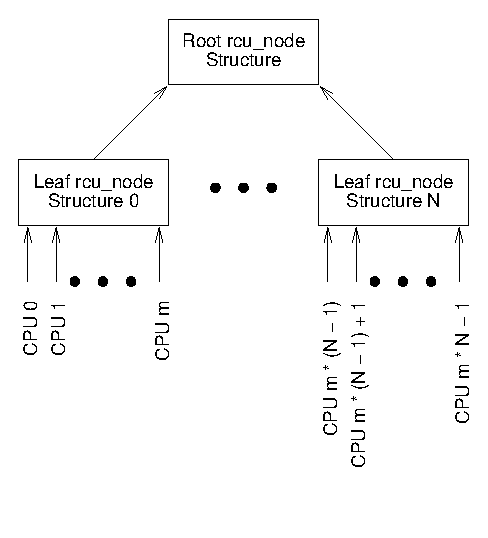
\includegraphics{locking/rnplock}}
\end{center}
\caption{Locking Hierarchy}
\label{fig:lock:Locking Hierarchy}
\end{figure}

Example data structures (taken from the Linux kernel's implementation
of RCU) are shown in
Figure~\ref{fig:lock:Locking Hierarchy}.
Here, each CPU is assigned a leaf \co{rcu_node} structure, and each
\co{rcu_node} structure has a pointer to its parent (named, oddly
enough, \co{->parent}), up to the root \co{rcu_node} structure,
which has a \co{NULL} \co{->parent} pointer.
The number of child \co{rcu_node} structures per parent can vary,
but is typically 32 or 64.
Each \co{rcu_node} structure also contains a lock named \co{->fqslock}.

The general approach is a \emph{tournament}, where
a given CPU conditionally acquires its
leaf \co{rcu_node} structure's \co{->fqslock}, and, if successful,
attempt to acquire that of the parent, then release that of the child.
In addition, at each level, the CPU checks a global \co{gp_flags}
variable, and if this variable indicates that some other CPU has
asserted the event, the first CPU drops out of the competition.
This acquire-then-release sequence continues until either the
\co{gp_flags} variable indicates that someone else won the tournament,
one of the attempts to acquire an \co{->fqslock} fails, or
the root \co{rcu_node} structure's \co{->fqslock} as been acquired.

\begin{figure}[tbp]
{ \scriptsize
\begin{verbatim}
  1 void force_quiescent_state(struct rcu_node *rnp_leaf)
  2 {
  3   int ret;
  4   struct rcu_node *rnp = rnp_leaf;
  5   struct rcu_node *rnp_old = NULL;
  6 
  7   for (; rnp != NULL; rnp = rnp->parent) {
  8     ret = (ACCESS_ONCE(gp_flags)) ||
  9           !raw_spin_trylock(&rnp->fqslock);
 10     if (rnp_old != NULL)
 11       raw_spin_unlock(&rnp_old->fqslock);
 12     if (ret)
 13       return;
 14     rnp_old = rnp;
 15   }
 16   if (ACCESS_ONCE(gp_flags)) {
 17     gp_flags = 1;
 18     do_force_quiescent_state();
 19     gp_flags = 0;
 20   }
 21   raw_spin_unlock(&rnp_old->fqslock);
 22 }
\end{verbatim}
}
\caption{Conditional Locking to Reduce Contention}
\label{fig:locking:Conditional Locking to Reduce Contention}
\end{figure}

Simplified code to implement this is shown in
Figure~\ref{fig:locking:Conditional Locking to Reduce Contention}.
The purpose of this function is to mediate between CPUs who have concurrently
detected a need to invoke the \co{do_force_quiescent_state()} function.
At any given time, it only makes sense for one instance of
\co{do_force_quiescent_state()} to be active, so if there are multiple
concurrent callers, we need at most one of them to actually invoke
\co{do_force_quiescent_state()}, and we need the rest to (as quickly and
painlessly as possible) give up and leave.

To this end, each pass through the loop spanning lines~7-15 attempts
to advance up one level in the \co{rcu_node} hierarcy.
If the \co{gp_flags} variable is already set (line~8) or if the attempt
to acquire the current \co{rcu_node} structure's \co{->fqslock} is
unsuccessful (line~9), then local variable \co{ret} is set to 1.
If line~10 sees that local variable \co{rnp_old} is non-\co{NULL},
meaning that we hold \co{rnp_old}'s \co{->fqs_lock},
line~11 releases this lock (but only after the attempt has been made
to acquire the parent \co{rcu_node} structure's \co{->fqslock}).
If line~12 sees that either line~8 or~9 saw a reason to give up,
line~13 returns to the caller.
Otherwise, we must have acquired the current \co{rcu_node} structure's
\co{->fqslock}, so line~14 saves a pointer to this structure in local
variable \co{rnp_old} in preparation for the next pass through the loop.

If control reaches line~16, we won the tournament, and now holds the
root \co{rcu_node} structure's \co{->fqslock}.
If line~16 still sees that the global variable \co{gp_flags} is zero,
line~17 sets \co{gp_flags} to one, line~18 invokes
\co{do_force_quiescent_state()}, and line~19 resets \co{gp_flags}
back to zero.
Either way, line~21 releases the root \co{rcu_node} structure's
\co{->fqslock}.

\QuickQuiz{}
	The code in
	Figure~\ref{fig:locking:Conditional Locking to Reduce Contention}
	is ridiculously complicated!
	Why not conditionally acquire a single global lock?
\QuickQuizAnswer{
	Conditionally acquiring a single global lock does work very well,
	but only for relatively small numbers of CPUs.
	To see why it is problematic in systems with many hundreds of
	CPUs, look at
	Figure~\ref{fig:count:Atomic Increment Scalability on Nehalem}
	and extrapolate the delay from eight to 1,000 CPUs.
} \QuickQuizEnd

\QuickQuiz{}
	Wait a minute!
	If we ``win'' the tournament on line~16 of
	Figure~\ref{fig:locking:Conditional Locking to Reduce Contention},
	we get to do all the work of \co{do_force_quiescent_state()}.
	Exactly how is that a win, really?
\QuickQuizAnswer{
	How indeed?
	This just shows that in concurrency, just as in life, one
	should take care to learn exactly what winning entails before
	playing the game.
} \QuickQuizEnd

This function illustrates the not-uncommon pattern of hierarchical
locking.
This pattern is quite difficult to implement using RAII locking,
just like the interator encapsulation noted earlier,
and so the lock/unlock primitives will be needed for the foreseeable
future.

\section{Locking Implementation Issues}
\label{sec:locking:Locking Implementation Issues}

Developers are almost always best-served by using whatever locking
primitives are provided by the system, for example, the POSIX
pthread mutex locks~\cite{OpenGroup1997pthreads,Butenhof1997pthreads}.
Nevertheless, studying sample implementations can be helpful,
as can considering the challenges posed by extreme workloads and
environments.

\subsection{Sample Exclusive-Locking Implementation Based on Atomic Exchange}
\label{sec:locking:Sample Exclusive-Locking Implementation Based on Atomic Exchange}

\begin{figure}[tbp]
{ \scriptsize
\begin{verbatim}
  1 typedef int xchglock_t;
  2 #define DEFINE_XCHG_LOCK(n) xchglock_t n = 0
  3 
  4 void xchg_lock(xchglock_t *xp)
  5 {
  6   while (xchg(xp, 1) == 1) {
  7     while (*xp == 1)
  8       continue;
  9   }
 10 }
 11 
 12 void xchg_unlock(xchglock_t *xp)
 13 {
 14   (void)xchg(xp, 0);
 15 }
\end{verbatim}
}
\caption{Sample Lock Based on Atomic Exchange}
\label{fig:locking:Sample Lock Based on Atomic Exchange}
\end{figure}

This section reviews the implementation shown in
Figure~\ref{fig:locking:Sample Lock Based on Atomic Exchange}.
The data structure for this lock is just an \co{int}, as shown on
line~1, but could be any integral type.
The initial value of this lock is zero, meaning ``unlocked'',
as shown on line~2.

\QuickQuiz{}
	Why not rely on the C language's default initialization of
	zero instead of using the explicit initializer shown on
	line~2 of
	Figure~\ref{fig:locking:Sample Lock Based on Atomic Exchange}?
\QuickQuizAnswer{
	Because this default initialization does not apply to locks
	allocated as auto variables within the scope of a function.
} \QuickQuizEnd

Lock acquisition is carried out by the \co{xchg_lock()} function
shown on lines~4-9.
This function uses a nested loop, with the outer loop repeatedly
atomically exchanging the value of the lock with the value one
(meaning ``locked'').
If the old value was already the value one (in other words, someone
else already holds the lock), then the inner loop (lines~7-8)
spins until the lock is available, at which point the outer loop
makes another attempt to acquire the lock.

\QuickQuiz{}
	Why bother with the inner loop on lines~7-8 of
	Figure~\ref{fig:locking:Sample Lock Based on Atomic Exchange}?
	Why not simply repeatedly do the atomic exchange operation
	on line~6?
\QuickQuizAnswer{
	Suppose that the lock is held and that several threads
	are attempting to acquire the lock.
	In this situation, if these threads all loop on the atomic
	exchange operation, they will ping-pong the cache line
	containing the lock among themselves, imposing load
	on the interconnect.
	In contrast, if these threads are spinning in the inner
	loop on lines~7-8, they will each spin within their own
	caches, putting negligible load on the interconnect.
} \QuickQuizEnd

Lock release is carried out by the \co{xchg_unlock()} function
shown on lines~12-15.
Line~14 atomically exchanges the value zero (``unlocked'') into
the lock, thus marking it as having been released.

\QuickQuiz{}
	Why not simply store zero into the lock word on line 14 of
	Figure~\ref{fig:locking:Sample Lock Based on Atomic Exchange}?
\QuickQuizAnswer{
	This can be a legitimate implementation, but only if
	this store is preceded by a memory barrier and makes use
	of \co{ACCESS_ONCE()}.
	The memory barrier is not required when the \co{xchg()}
	operation is used because this operation implies a
	full memory barrier due to the fact that it returns
	a value.
} \QuickQuizEnd

This lock is a simple example of a test-and-set lock~\cite{Segall84},
but very similar
mechanisms have been used extensively as pure spinlocks in production.

\subsection{Other Exclusive-Locking Implementations}
\label{sec:locking:Other Exclusive-Locking Implementations}

There are a great many other possible implementations of locking
based on atomic instructions, many of which are reviewed
by Mellor-Crummey and Scott~\cite{MellorCrummey91a}.
These implementations represent different points in a multi-dimensional
design tradeoff~\cite{McKenney96a}.
For example,
the atomic-exchange-based test-and-set lock presented in the previous
section works well when contention is low and has the advantage
of small memory footprint.
It avoids giving the lock to threads that cannot use it, but as
a result can suffer from unfairness or even starvation at high
contention levels.

In contrast, ticket lock~\cite{MellorCrummey91a}, which is used in the Linux
kernel, avoids unfairness at high contention levels, but as a
consequence of its first-in-first-out discipline can grant the
lock to a thread that is currently unable to use it, for example,
due to being preempted, interrupted, or otherwise out of action.
However, it is important to avoid getting too worried about the
possibility of preemption and interruption, given that this preemption
and interruption might just as well happen just after the lock was
acquired.\footnote{
	Besides, the best way of handling high lock contention is to avoid
	it in the first place!
	However, there are some situation where high lock contention
	is the lesser of the available evils, and in any case, studying
	schemes that deal with high levels of contention is good mental
	exercise.}

All locking implementations where waiters spin on a single memory
location, including both test-and-set locks and ticket locks,
suffer from performance problems at high contention levels.
The problem is that the thread releasing the lock must update the
value of the corresponding memory location.
At low contention, this is not a problem: The corresponding cache line
is very likely still local to and writeable by the thread holding
the lock.
In contrast, at high levels of contention, each thread attempting to
acquire the lock will have a read-only copy of the cache line, and
the lock holder will need to invalidate all such copies before it
can carry out the update that releases the lock.
In general, the more CPUs and threads there are, the greater the
overhead incurred when releasing the lock under conditions of
high contention.

This negative scalability has motivated a number of different
queued-lock
implementations~\cite{Anderson90,Graunke90,MellorCrummey91a,Wisniewski94,Craig93,Magnusson94,Takada93},
which assign different queue elements to each of the threads attempting
to acquire the lock, thus reducing the lock's memory contention.

More recent queued-lock implementations also take the system's architecture
into account, preferentially granting locks locally, while also taking
steps to avoid
starvation~\cite{McKenney02e,radovic03hierarchical,radovic02efficient,BenJackson02,McKenney02d}.
Many of these can be thought of as analogous to the elevator algorithms
traditionally used in scheduling disk I/O.

Unfortunately, the same scheduling logic that improves the efficiency
of queued locks at high contention also increases their overhead at
low contention.
Beng-hong Lim and Anant Agarwal therefore combined a simple test-and-set
lock with a queued lock, using the test-and-set lock at low levels of
contention and switching to the queued lock at high levels of
contention~\cite{BengHongLim94}, thus getting low overhead at low levels
of contention and getting fairness and high throughput at high levels
of contention.
Browning et al.~took a similar approach, but avoided the use of a separate
flag, so that the test-and-set fast path uses the same sequence of
instructions that would be used in a simple test-and-set
lock~\cite{LukeBrowning2005SimpleLockNUMAAware}.
This approach has been used in production.

Another issue that arises at high levels of contention is when the
lock holder is delayed, especially when the delay is due to
preemption, which can result in \emph{priority inversion},
where a low-priority thread holds a lock, but is preempted
by a medium priority CPU-bound thread, which results in
a high-priority process blocking while attempting to acquire the
lock.
The result is that the CPU-bound medium-priority process is preventing the
high-priority process from running.
One solution is \emph{priority inheritance}~\cite{Lampson1980Mesa},
which has been widely used for real-time
computing~\cite{Sha1990IEEETransComp,JonathanCorbet2006PriorityInheritance},
despite some lingering controversy over this
practice~\cite{Yodaiken2004FSM,DougLocke2002a}.

Another way to avoid priority inversion is to prevent preemption
while a lock is held.
Because preventing preemption while locks are held also improves throughput,
most proprietary UNIX kernels offer some form of scheduler-conscious
synchronization mechanism~\cite{Kontothanassis97a},
largely due to the efforts of a certain sizable database vendor.
These mechanisms usually take the form of a hint that preemption
would be imappropriate.
These hints frequently take the form of a bit set in a particular
machine register, which enables extremely low per-lock-acquisition overhead
for these mechanisms.
In contrast, Linux avoids these hints, instead getting
similar results from a mechanism called
\emph{futexes}~\cite{HubertusFrancke2002Futex,IngoMolnar2006RobustFutexes,StevenRostedt2006piFutexes,UlrichDrepper2011Futexes}.

Interestingly enough, atomic instructions are not strictly needed to
implement locks~\cite{Dijkstra65a,Lamport74a}.
An excellent exposition of the issues surrounding locking implementations
based on simple loads and stores may be found in Herlihy's and
Shavit's textbook~\cite{HerlihyShavit2008Textbook}.
The main point echoed here is that such implementations currently
have little practical application, although a careful study of
them can be both entertaining and enlightening.
Nevertheless, with one exception described below, such study is left
as an exercise for the reader.

Gamsa et al.~\cite[Section 5.3]{Gamsa99} describe a token-based
mechanism in which a token circulates among the CPUs.
When the token reaches a given CPU, it has exclusive
access to anything protected by that token.
There are any number of schemes that may be used to implement
the token-based mechanism, for example:

\begin{enumerate}
\item	Maintain a per-CPU flag, which is initially
	zero for all but one CPU.
	When a CPU's flag is non-zero, it holds the token.
	When it finishes with the token, it zeroes its flag and
	sets the flag of the next CPU to one (or to any other
	non-zero value).
\item	Maintain a per-CPU counter, which is initially set
	to the corresponding CPU's number, which we assume
	to range from zero to $N-1$, where $N$ is the number
	of CPUs in the system.
	When a CPU's counter is greater than that of the next
	CPU (taking counter wrap into account), the first CPU holds the token.
	When it is finished with the token, it sets the next
	CPU's counter to a value one greater than its own counter.
\end{enumerate}

\QuickQuiz{}
	How can you tell if one counter is greater than another,
	while accounting for counter wrap?
\QuickQuizAnswer{
	In the C language, the following macro correctly handles this:

\vspace{5pt}
\begin{minipage}[t]{\columnwidth}
\small
\begin{verbatim}
#define ULONG_CMP_LT(a, b) \
        (ULONG_MAX / 2 < (a) - (b))
\end{verbatim}
\end{minipage}
\vspace{5pt}

	Although it is tempting to simply subtract two signed integers,
	this should be avoided because signed overflow is undefined
	in the C language.
	For example, if the compiler knows that one of the values is
	positive and the other negative, it is within its rights to
	simply assume that the positive number is greater than the
	negative number, even though subtracting the negative number
	from the positive number might well result in overflow and
	thus a negative number.

	How could the compiler know the signs of the two numbers?
	It might be able to deduce it based on prior assignments
	and comparisons.
	In this case, if the per-CPU counters were signed, the compiler
	could deduce that they were always increasing in value, and
	then might assume that they would never go negative.
	This assumption could well lead the compiler to generate
	unfortunate code~\cite{PaulEMcKenney2012SignedOverflow,JohnRegehr2010UndefinedBehavior}.
} \QuickQuizEnd

\QuickQuiz{}
	Which is better, the counter approach or the flag approach?
\QuickQuizAnswer{
	The flag approach will normally suffer fewer cache misses,
	but a better answer is to try both and see which works best
	for your particular workload.
} \QuickQuizEnd

This lock is unusual in that a given CPU cannot necessarily acquire it
immediately, even if no other CPU is using it at the moment.
Instead, the CPU must wait until the token comes around to it.
This is useful in cases where CPUs need periodic access to the critical
section, but can tolerate variances in token-circulation rate.
Gamsa et al.~\cite{Gamsa99} used it to implement a variant of
read-copy update (see Section~\ref{sec:defer:Read-Copy Update (RCU)}),
but it could also be used to protect periodic per-CPU operations such
as flushing per-CPU caches used by memory allocators~\cite{McKenney93},
garbage-collecting per-CPU data structures, or flushing per-CPU
data to shared storage (or to mass storage, for that matter).

As increasing numbers of people gain familiarity with parallel hardware
and parallelize increasing amounts of code, we can expect more
special-purpose locking primitives to appear.
Nevertheless, you should carefully consider this important safety tip:
Use the standard synchronization primitives whenever humanly possible.
The big advantage of the standard synchronization primitives over
roll-your-own efforts is that the standard primitives are typically
\emph{much} less bug-prone.\footnote{
	And yes, I have done at least my share of roll-your-own
	synchronization primitives.
	However, you will notice that my hair is much greyer than
	it was before I started doing that sort of work.
	Coincidence?
	Maybe.
	But are you \emph{really} willing to risk your own hair turning
	prematurely grey?}

% locking-existence.tex

\section{Lock-Based Existence Guarantees}
\label{sec:locking:Lock-Based Existence Guarantees}

{ \scriptsize
\begin{verbbox}
  1 int delete(int key)
  2 {
  3   int b;
  4   struct element *p;
  5
  6   b = hashfunction(key);
  7   p = hashtable[b];
  8   if (p == NULL || p->key != key)
  9     return 0;
 10   spin_lock(&p->lock);
 11   hashtable[b] = NULL;
 12   spin_unlock(&p->lock);
 13   kfree(p);
 14   return 1;
 15 }
\end{verbbox}
}
\begin{figure}[tbp]
\centering
\theverbbox
\caption{Per-Element Locking Without Existence Guarantees}
\label{fig:locking:Per-Element Locking Without Existence Guarantees}
\end{figure}

A key challenge in parallel programming is to provide
\emph{existence guarantees}~\cite{Gamsa99},
so that attempts to access a given object can rely on that object
being in existence throughout a given access attempt.
In some cases, existence guarantees are implicit:

\begin{enumerate}
\item	Global variables and static local variables in the base module
	will exist as long as the application is running.
\item	Global variables and static local variables in a loaded module
	will exist as long as that module remains loaded.
\item	A module will remain loaded as long as at least one of its functions
	has an active instance.
\item	A given function instance's on-stack variables will exist until
	that instance returns.
\item	If you are executing within a given function or have been
	called (directly or indirectly) from that function,
	then the given function has an active instance.
\end{enumerate}

These implicit existence guarantees are straightforward, though
bugs involving implicit existence guarantees really can happen.

\QuickQuiz{}
	How can relying on implicit existence guarantees result in
	a bug?
\QuickQuizAnswer{
	Here are some bugs resulting from improper use of implicit
	existence guarantees:
	\begin{enumerate}
	\item	A program writes the address of a global variable to
		a file, then a later instance of that same program
		reads that address and attempts to dereference it.
		This can fail due to address-space randomization,
		to say nothing of recompilation of the program.
	\item	A module can record the address of one of its variables
		in a pointer located in some other module, then attempt
		to dereference that pointer after the module has
		been unloaded.
	\item	A function can record the address of one of its on-stack
		variables into a global pointer, which some other
		function might attempt to dereference after that function
		has returned.
	\end{enumerate}
	I am sure that you can come up with additional possibilities.
} \QuickQuizEnd

But the more interesting---and troublesome---guarantee involves
heap memory: A dynamically allocated data structure will exist until it
is freed.
The problem to be solved is to synchronize the freeing of the structure
with concurrent accesses to that same structure.
One way to do this is with \emph{explicit guarantees}, such as locking.
If a given structure may only be freed while holding a given lock, then holding
that lock guarantees that structure's existence.

But this guarantee depends on the existence of the lock itself.
One straightforward way to guarantee the lock's existence is to
place the lock in a global variable, but global locking has the disadvantage
of limiting scalability.
One way of providing scalability that improves as the size of the
data structure increases is to place a lock in each element of the
structure.
Unfortunately, putting the lock that is to protect a data element
in the data element itself is subject to subtle race conditions,
as shown in
Figure~\ref{fig:locking:Per-Element Locking Without Existence Guarantees}.

\QuickQuiz{}
	What if the element we need to delete is not the first element
	of the list on line~8 of
	Figure~\ref{fig:locking:Per-Element Locking Without Existence Guarantees}?
\QuickQuizAnswer{
	This is a very simple hash table with no chaining, so the only
	element in a given bucket is the first element.
	The reader is invited to adapt this example to a hash table with
	full chaining.
} \QuickQuizEnd

\QuickQuiz{}
	What race condition can occur in
	Figure~\ref{fig:locking:Per-Element Locking Without Existence Guarantees}?
\QuickQuizAnswer{
	Consider the following sequence of events:
	\begin{enumerate}
	\item	Thread~0 invokes \co{delete(0)}, and reaches line~10 of
		the figure, acquiring the lock.
	\item	Thread~1 concurrently invokes \co{delete(0)}, reaching
		line~10, but spins on the lock because Thread~0 holds it.
	\item	Thread~0 executes lines~11-14, removing the element from
		the hashtable, releasing the lock, and then freeing the
		element.
	\item	Thread~0 continues execution, and allocates memory, getting
		the exact block of memory that it just freed.
	\item	Thread~0 then initializes this block of memory as some
		other type of structure.
	\item	Thread~1's \co{spin_lock()} operation fails due to the
		fact that what it believes to be \co{p->lock} is no longer
		a spinlock.
	\end{enumerate}
	Because there is no existence guarantee, the identity of the
	data element can change while a thread is attempting to acquire
	that element's lock on line~10!
} \QuickQuizEnd

{ \scriptsize
\begin{verbbox}
  1 int delete(int key)
  2 {
  3   int b;
  4   struct element *p;
  5   spinlock_t *sp;
  6
  7   b = hashfunction(key);
  8   sp = &locktable[b];
  9   spin_lock(sp);
 10   p = hashtable[b];
 11   if (p == NULL || p->key != key) {
 12     spin_unlock(sp);
 13     return 0;
 14   }
 15   hashtable[b] = NULL;
 16   spin_unlock(sp);
 17   kfree(p);
 18   return 1;
 19 }
\end{verbbox}
}
\begin{figure}[tbp]
\centering
\theverbbox
\caption{Per-Element Locking With Lock-Based Existence Guarantees}
\label{fig:locking:Per-Element Locking With Lock-Based Existence Guarantees}
\end{figure}

One way to fix this example is to use a hashed set of global locks, so
that each hash bucket has its own lock, as shown in
Figure~\ref{fig:locking:Per-Element Locking With Lock-Based Existence Guarantees}.
This approach allows acquiring the proper lock (on line~9) before
gaining a pointer to the data element (on line~10).
Although this approach works quite well for elements contained in a
single partitionable data structure such as the hash table shown in the
figure, it can be problematic if a given data element can be a member
of multiple hash tables or given more-complex data structures such
as trees or graphs.
These problems can be solved, in fact, such solutions form the basis
of lock-based software transactional memory
implementations~\cite{Shavit95,DaveDice2006DISC}.
However,
Chapter~\ref{chp:Deferred Processing}
describes simpler---and faster---ways of providing existence guarantees.


\section{Locking: Hero or Villain?}
\label{sec:locking:Locking: Hero or Villain?}

As is often the case in real life, locking can be either hero or villain,
depending on how it is used and on the problem at hand.
In my experience, those writing whole applications are happy with
locking, those writing parallel libraries are less happy, and those
parallelizing existing sequential libraries are extremely unhappy.
The following sections discuss some reasons for these differences in
viewpoints.

\subsection{Locking For Applications: Hero!}
\label{sec:locking:Locking For Applications: Hero!}

When writing an entire application (or entire kernel), developers have
full control of the design, including the synchronization design.
Assuming that the design makes good use of partitioning, as discussed in
Chapter~\ref{cha:Partitioning and Synchronization Design}, locking
can be an extremely effective synchronization mechanism, as demonstrated
by the heavy use of locking in production-quality parallel software.

Nevertheless, although such software usually bases most of its
synchronization design on locking, such software also almost always
makes use of other synchronization mechanisms, including
special counting algorithms (Chapter~\ref{chp:Counting}),
data ownership (Chapter~\ref{chp:Data Ownership}),
reference counting (Section~\ref{sec:defer:Reference Counting}), 
sequence locking (Section~\ref{sec:defer:Sequence Locks}), and
read-copy update (Section~\ref{sec:defer:Read-Copy Update (RCU)}).
In addition, practitioners use tools for deadlock
detection~\cite{JonathanCorbet2006lockdep},
lock acquisition/release balancing~\cite{JonathanCorbet2004sparse},
cache-miss analysis~\cite{ValgrindHomePage},
hardware-counter-based profiling~\cite{LinuxKernelPerfWiki,OProfileHomePage},
and many more besides.

Given careful design, use of a good combination of synchronization
mechanisms, and good tooling, locking works quite well for applications
and kernels.

\subsection{Locking For Parallel Libraries: Just Another Tool}
\label{sec:locking:Locking For Parallel Libraries: Just Another Tool}

Unlike applications and kernels, the designer of a library cannot
know the locking design of the code that the library will be interacting
with.
In fact, that code might not be written for years to come.
Library designers therefore have less control and must exercise more
care when laying out their synchronization design.

Deadlock is of course of particular concern, and the techniques discussed
in Section~\ref{sec:locking:Deadlock} need to be applied.
One popular deadlock-avoidance strategy is therefore to ensure that
the library's locks are independent subtrees of the enclosing program's
locking hierarchy.
However, this can be harder than it looks.

One complication was discussed in
Section~\ref{sec:locking:Local Locking Hierarchies}, namely
when library functions call into application code, with \co{qsort()}'s
comparison-function argument being a case in point.
Another complication is the interaction with signal handlers.
If an application signal handler is invoked from a signal received within
the library function, deadlock can ensue just as surely as
if the library function had called the signal handler directly.
A final complication occurs for those library functions that can be used
between a \co{fork()}/\co{exec()} pair, for example, due to use of
the \co{system()} function.
In this case, if your library function was holding a lock at the time of
the \co{fork()}, then the child process will begin life with that lock held.
Because the thread that will release the lock is running in the parent
but not the child, if the child calls your library function, deadlock
will ensue.

The following strategies may be used to avoid deadlock problems in these cases:

\begin{enumerate}
\item	Don't use either callbacks or signals.
\item	Don't acquire locks from within callbacks or signal handlers.
\item	Let the caller control synchronization.
\item	Parameterize the library API to delegate locking to caller.
\item	Explicitly avoid callback deadlocks.
\item	Explicitly avoid signal-handler deadlocks.
\end{enumerate}

Each of these strategies is discussed in on of the following sections.

\subsubsection{Use Neither Callbacks Nor Signals}
\label{sec:locking:Use Neither Callbacks Nor Signals}

If a library function avoids callbacks and the application as a whole
avoids signals, then any locks acquired by that library function will
be leaves of the locking-hierarchy tree.
This arrangement avoids deadlock, as discussed in
Section~\ref{sec:locking:Locking Hierarchies}.
Although this strategy works extremely well where it applies,
there are some applications that must use signal handlers,
and there are some library functions (such as the \co{qsort()} function
discussed in
Section~\ref{sec:locking:Local Locking Hierarchies})
that require callbacks.

The strategy described in the next section can often be used in these cases.

\subsubsection{Avoid Locking in Callbacks and Signal Handlers}
\label{sec:locking:Avoid Locking in Callbacks and Signal Handlers}

If neither callbacks nor signal handlers acquire locks, then they
cannot be involved in deadlock cycles, which allows straightforward
locking hierarchies to once again consider library functions to
be leaves on the locking-hierarchy tree.
This strategy works very well for most uses of \co{qsort}, whose
callbacks usually simply compare the two values passed in to them.
This strategy also works wonderfully for many signal handlers,
especially given that acquiring locks from within signal handlers
is generally frowned upon~\cite{TheOpenGroup1997SUS},\footnote{
	But the standard's words do not stop clever coders from creating
	their own home-brew locking primitives from atomic operations.}
but can fail if the application needs to manipulate complex data structures
from a signal handler.

Here are some ways to avoid acquiring locks in signal handlers even
if complex data structures must be manipulated:

\begin{enumerate}
\item	Use simple data structures based on non-blocking synchronization,
	as will be discussed in
	Section~\ref{sec:advsync:Simple NBS}.
\item	If the data structures are too complex for reasonable use of
	non-blocking synchronization, create a queue that allows
	non-blocking enqueue operations.
	In the signal handler, instead of manipulating the complex
	data structure, add an element to the queue describing the
	required change.
	A separate thread can then remove elements from the queue and
	carry out the required changes using normal locking.
	There are a number of readily available implementations of
	concurrent
	queues~\cite{ChristophMKirsch2012FIFOisntTR,MathieuDesnoyers2009URCU,MichaelScott96}.
\end{enumerate}

This strategy should be enforced with occasional manual or (preferably)
automated inspections of callbacks and signal handlers.
When carrying out these inspections, be wary of clever coders who
might have (unwisely) created home-brew locks from atomic operations.

\subsubsection{Caller Controls Synchronization}
\label{sec:locking:Caller Controls Synchronization}

Let the caller control synchronization.
This works extremely well when the library functions are operating
on independent caller-visible instances of a data structure, each
of which may be synchronized separately.
For example, if the library functions operate on a search tree,
and if the application needs a large number of independent search
trees, then the application can associate a lock with each tree.
The application then acquires and releases locks as needed, so
that the library need not be aware of parallelism at all.
Instead, the application controls the parallelism, so that locking
can work very well, as was discussed in
Section~\ref{sec:locking:Locking For Applications: Hero!}.

However, this strategy fails if the
library implements a data structure that requires internal
concurrency, for example, a hash table or a parallel sort.
In this case, the library absolutely must control its own
synchronization.

\subsubsection{Parameterize Library Synchronization}
\label{sec:locking:Parameterize Library Synchronization}

The idea here is to add arguments to the library's API to specify
which locks to acquire, how to acquire and release them, or both.
This strategy allows the application to take on the global task of
avoiding deadlock by specifying which locks to acquire (by passing in
pointers to the locks in question) and how to
acquire them (by passing in pointers to lock acquisition and release
functions),
but also allows a given library function to control its own concurrency
by deciding where the locks should be acquired and released.

In particular, this strategy allows the lock acquisition and release
functions to block signals as needed without the library code needing to
be concerned with of which signals need to be blocked by which locks.
The separation of concerns used by this strategy can be quite effective,
but in some cases the strategies laid out in the following sections
can work better.

That said, passing explicit pointers to locks to external APIs must
be very carefully considered, as discussed in
Section~\ref{sec:locking:Locking Hierarchies and Pointers to Locks}.
Although this practice is sometimes the right thing to do, you should do
yourself a favor by looking into alternative designs first.

\subsubsection{Explicitly Avoid Callback Deadlocks}
\label{sec:locking:Explicitly Avoid Callback Deadlocks}

The basic rule behind this strategy was discussed in
Section~\ref{sec:locking:Local Locking Hierarchies}: ``Release all
locks before invoking unknown code.''
This is usually the best approach because it allows the application to
ignore the library's locking hierarchy: the library remains a leaf or
isolated subtree of the application's overall locking hierarchy.

In cases where it is not possible to release all locks before invoking
unknown code, the layered locking hierarchies described in
Section~\ref{sec:locking:Layered Locking Hierarchies} can work well.
For example, if the unknown code is a signal handler, this implies that
the library function block signals across all lock acquisitions, which
can be complex and slow.
Therefore, in cases where signal handlers (probably unwisely) acquire
locks, the strategies in the next section may prove helpful.

\subsubsection{Explicitly Avoid Signal-Handler Deadlocks}
\label{sec:locking:Explicitly Avoid Signal-Handler Deadlocks}

Signal-handler deadlocks can be explicitly avoided as follows:

\begin{enumerate}
\item	If the application invokes the library function from
	within a signal handler, then that signal must be blocked
	every time that the library function is invoked from outside
	of a signal handler.
\item	If the application invokes the library function
	while holding a lock acquired within a given signal
	handler, then that signal must be blocked every time that the
	library function is called outside of a signal handler.
\end{enumerate}

These rules can be enforced by using tools similar to
the Linux kernel's lockdep lock dependency
checker~\cite{JonathanCorbet2006lockdep}.
One of the great strengths of lockdep is that it is not fooled by
human intuition~\cite{StevenRostedt2011locdepCryptic}.

\subsubsection{Library Functions Used Between fork() and exec()}
\label{sec:locking:Library Functions Used Between fork() and exec()}

As noted earlier, if a thread executing a library function is holding
a lock at the time that some other thread invokes \co{fork()}, the
fact that the parent's memory is copied to create the child means that
this lock will be born held in the child's context.
The thread that will release this lock is running in the parent, but not
in the child, which means that the child's copy of this lock will never
be released.
Therefore, any attempt on the part of the child to invoke that same
library function will result in deadlock.

One approach to this problem would be to have the library function
check to see if the owner of the lock is still running, and if not,
``breaking'' the lock by re-initializing and then acquiring it.
However, this approach has a couple of vulnerabilities:

\begin{enumerate}
\item	The data structures protected by that lock are likely to
	be in some intermediate state, so that naively breaking the lock
	might result in arbitrary memory corruption.
\item	If the child creates additional threads, two threads might
	break the lock concurrently, with the result that both
	threads believe they own the lock.
	This could again result in arbitrary memory corruption.
\end{enumerate}

The \co{atfork()} function is provided to help deal with these situations.
The idea is to register a triplet of functions, one to be called by the
parent before the \co{fork()}, one to be called by the parent after the
\co{fork()}, and one to be called by the child after the \co{fork()}.
Appropriate cleanups can then be carried out at these three points.

Be warned, however, that coding of \co{atfork()} handlers is quite subtle
in general.
The cases where \co{atfork()} works best are cases where the data structure
in question can simply be re-initialized by the child.

\subsubsection{Parallel Libraries: Discussion}
\label{sec:locking:Parallel Libraries: Discussion}

Regardless of the strategy used, the description of the library's API
must include a clear description of that strategy and how the caller
should interact with that strategy.
In short, constructing parallel libraries using locking is possible,
but not as easy as constructing a parallel application.

\subsection{Locking For Parallelizing Sequential Libraries: Villain!}
\label{sec:locking:Locking For Parallelizing Sequential Libraries: Villain!}

With the advent of readily available low-cost multicore systems,
a common task is parallelizing an existing library that was designed
with only single-threaded use in mind.
This all-to-common disregard for parallelism can result in a library
API that is severely flawed from a parallel-programming viewpoint.
Candidate flaws include:

\begin{enumerate}
\item	Implicit prohibition of partitioning.
\item	Callback functions requiring locking.
\item	Object-oriented spaghetti code.
\end{enumerate}

These flaws and the consequences for locking are discussed in the following
sections.

\subsubsection{Partitioning Prohibited}
\label{sec:locking:Partitioning Prohibited}

Suppose that you were writing a single-threaded hash-table implementation.
It is easy and fast to maintain an exact count of the total number of items
in the hash table, and also easy and fast to return this exact count on each
addition and deletion operation.
So why not?

One reason is that exact counters do not perform or scale well on
multicore systems, as was
seen in Chapter~\ref{chp:Counting}.
As a result, the parallelized implementation of the hash table will not
perform or scale well.

So what can be done about this?
One approach is to return an approximate count, using one of the algorithms
from Chapter~\ref{chp:Counting}.
Another approach is to drop the element count altogether.

Either way, it will be necessary to inspect uses of the hash table to see
why the addition and deletion operations need the exact count.
Here are a few possibilities:

\begin{enumerate}
\item	Determining when to resize the hash table.
	In this case, an approximate count should work quite well.
	It might also be useful to trigger the resizing operation from
	the length of the longest chain, which can be computed and
	maintained in a nicely partitioned per-chain manner.
\item	Producing an estimate of the time required to traverse the
	entire hash table.
	An approximate count works well in this case, also.
\item	For diagnostic purposes, for example, to check for items being
	lost when transferring them to and from the hash table.
	This clearly requires an exact count.
	However, given that this usage is diagnostic in nature, it might
	suffice to maintain the lengths of the hash chains, then to
	infrequently sum them
	up while locking out addition and deletion operations.
\end{enumerate}

It turns out that there is now a strong theoretical basis for some of the
constraints that performance and scalability place on a parallel library's
APIs~\cite{HagitAttiya2011LawsOfOrder,PaulEMcKenney2011SNC}.
Anyone designing a parallel library needs to pay close attention to
those constraints.

Although it is all too easy to blame locking for what are really problems
due to a concurrency-unfriendly API, doing so is not helpful.
On the other hand, one has little choice but to sympathize with the
hapless developer who made this choice in (say) 1985.
It would have been a rare and courageous developer to anticipate the
need for parallelism at that time, and it would have required an
even more rare combination of brilliance and luck to actually arrive
at a good parallel-friendly API.

Times change, and code must change with them.
That said, there might be a huge number of users of a popular library,
in which case an incompatible change to the API would be quite foolish.
Adding a parallel-friendly API to complement the existing heavily used
sequential-only API is probably the best course of action in this
situation.

Nevertheless, human nature being what it is, we can expect our hapless
developer to be more likely to complain about locking than about his
or her own poor (though understandable) API design choices.

\subsubsection{Deadlock-Prone Callbacks}
\label{sec:locking:Deadlock-Prone Callbacks}

Sections~\ref{sec:locking:Local Locking Hierarchies},
\ref{sec:locking:Layered Locking Hierarchies},
and~\ref{sec:locking:Locking For Parallel Libraries: Just Another Tool}
described how undisciplined use of callbacks can result in locking
woes.
These sections also described how to design your library function to
avoid these problems, but it is unrealistic to expect a 1990s programmer
with no experience in parallel programming to have followed such a design.
Therefore, someone attempting to parallelize an existing callback-heavy
single-threaded library will likely have many opportunities to curse
locking's villainy.

If there are a very large number of uses of a callback-heavy library,
it may be wise to again add a parallel-friendly API to the library in
order to allow existing users to convert their code incrementally.
Alternatively, some advocate use of transactional memory in these cases.
While the jury is still out on transactional memory,
Section~\ref{sec:future:Transactional Memory} discusses its strengths and
weaknesses.
It is important to note that hardware transactional memory
(discussed in
Section~\ref{sec:future:Hardware Transactional Memory})
cannot help here unless the hardware transactional memory implementation
provides forward-progress guarantees, which few do.
Other alternatives that appear to be quite practical (if less heavily
hyped) include the methods discussed in
Sections~\ref{sec:locking:Conditional Locking},
and~\ref{sec:locking:Acquire Needed Locks First},
as well as those that will be discussed in
Chapters~\ref{chp:Data Ownership}
and~\ref{chp:Deferred Processing}.

\subsubsection{Object-Oriented Spaghetti Code}
\label{sec:locking:Object-Oriented Spaghetti Code}

Object-oriented programming went mainstream sometime in the 1980s or
1990s, and as a result there is a huge amount of object-oriented code
in production, much of it single-threaded.
Although object orientation can be a valuable software technique,
undisciplined use of objects can easily result in object-oriented
spaghetti code.
In object-oriented spaghetti code, control flits from object to object
in an essentially random manner, making the code hard to understand
and even harder, and perhaps impossible, to accommodate a locking hierarchy.

Although many might argue that such code should be cleaned up in any
case, such things are much easier to say than to do.
If you are tasked with parallelizing such a beast, you can reduce the
number of opportunities to curse locking by using the techniques
described in
Sections~\ref{sec:locking:Conditional Locking},
and~\ref{sec:locking:Acquire Needed Locks First},
as well as those that will be discussed in
Chapters~\ref{chp:Data Ownership}
and~\ref{chp:Deferred Processing}.
This situation appears to be the use case that inspired transactional
memory, so it might be worth a try as well.

But there is one question well worth asking in these situations:
Should the code remain sequential?
For example, perhaps parallelism should be introduced at the process level
rather than the thread level.
In general, if a task is proving extremely hard, it is worth some time
spent thinking about not only alternative ways to accomplish that
particular task, but also alternative tasks that might better solve
the problem at hand.

\section{Summary}
\label{sec:locking:Summary}

Locking is perhaps the most widely used and most generally useful
synchronization tool.
However, it works best when designed into an application
or library from the beginning.
Given the large quantity of pre-existing single-threaded code that might
need to one day run in parallel, locking should therefore not be the
only tool in your parallel-programming toolbox.
The next few chapters will discuss other tools, and how they can best
be used in concert with locking and with each other.

% owned/owned.tex

\QuickQuizChapter{chp:Data Ownership}{Data Ownership}

One of the simplest ways to avoid the synchronization overhead that
comes with locking is to parcel the data out among the threads (or,
in the case of kernels, CPUs)
so that a given piece of data is accessed and modified by only one
of the threads.
This approach is used extremely heavily, in fact, it is one usage
pattern that even novices use almost instinctively.
In fact, it is used so heavily that this chapter will not introduce
any new examples, but will instead recycle examples from previous
chapters.

\QuickQuiz{}
	What form of data ownership that is extremely difficult
	to avoid using when creating shared-memory parallel programs
	(for example, using pthreads) in C or C++?
\QuickQuizAnswer{
	Use of auto variables in functions.
	By default, these are private to the thread executing the
	current function.
} \QuickQuizEnd

@@@ Roadmap

\section{Multiple Processes}
\label{sec:owned:Multiple Processes}

Section~\ref{sec:toolsoftrade:Scripting Languages}
introduced the following example:

\vspace{5pt}
\begin{minipage}[t]{\columnwidth}
\scriptsize
\begin{verbatim}
  1 compute_it 1 > compute_it.1.out &
  2 compute_it 2 > compute_it.2.out &
  3 wait
  4 cat compute_it.1.out
  5 cat compute_it.2.out
\end{verbatim}
\end{minipage}
\vspace{5pt}

This example runs two instances of the \co{compute_it} program in
parallel, as separate processes that do not share memory.
Therefore, all data in a given process is owned by that process,
so that almost the entirety of data in the above example is owned.
This approach almost entirely eliminates synchronization overhead.
The resulting combination of extreme simplicity and optimal performance
is obviously quite attractive.

\QuickQuiz{}
	What synchronization remains in the example shown in
	Section~\ref{sec:owned:Multiple Processes}?
\QuickQuizAnswer{
	The creation of the threads via the \co{sh} \co{&} operator
	and the joining of thread via the \co{sh} \co{wait}
	command.

	Of course, if the processes explicitly share memory, for
	example, using the \co{shmget()} or \co{mmap()} system
	calls, explicit synchronization might well be needed when
	acccessing or updating the shared memory.
	The processes might also synchronize using any of the following
	interprocess communications mechanisms:
	\begin{enumerate}
	\item	System V semaphores.
	\item	System V message queues.
	\item	UNIX-domain sockets.
	\item	Networking protocols, including TCP/IP, UDP, and a whole
		host of others.
	\item	File locking.
	\item	Use of the \co{open()} system call with the
		\co{O_CREAT} and \co{O_EXCL} flags.
	\item	Use of the \co{rename()} system call.
	\end{enumerate}
	A complete list of possible synchronization mechanisms is left
	as an exercise to the reader, who is warned that it will be
	an extremely long list.
	A surprising number of unassuming system calls can be pressed
	into service as synchronization mechanisms.
} \QuickQuizEnd

\QuickQuiz{}
	Is there any shared data in the example shown in
	Section~\ref{sec:owned:Multiple Processes}?
\QuickQuizAnswer{
	That is a philosophical question.

	Those wishing the answer ``no'' might argue that processes by
	definition do not share memory.

	Those wishing to answer ``yes'' might list a large number of
	synchronization mechanisms that do not require shared memory,
	note that the kernel will have some shared state, and perhaps
	even argue that the assignment of process IDs (PIDs) constitute
	shared data.

	Such arguments are excellent intellectual exercise, and are
	also a wonderful way of feeling intelligent, scoring points
	against hapless classmates or colleagues,
	and (especially!) avoiding getting anything useful done.
} \QuickQuizEnd

This same pattern can be written in C as well as in \co{sh}, as illustrated by
Figures~\ref{fig:toolsoftrade:Using the fork() Primitive}
and~\ref{fig:toolsoftrade:Using the wait() Primitive}.

The next section discusses use of data ownership in shared-memory
parallel programs.

\section{Partial Data Ownership and pthreads}
\label{sec:owned:Partial Data Ownership and pthreads}

Chapter~\ref{chp:Counting} makes heavy use of data ownership,
but adds a twist.
Threads are not allowed to modify data owned by other threads,
but they are permitted to read it.
In short, the use of shared memory allows more nuanced notions
of ownership and access rights.

For example, consider the per-thread statistical counter implementation
shown in
Figure~\ref{fig:count:Per-Thread Statistical Counters} on
page~\pageref{fig:count:Per-Thread Statistical Counters}.
Here, \co{inc_count()} updates only the corresponding thread's
instance of \co{counter},
while \co{read_count()} accesses, but does not modify, all
threads' instances of \co{counter}.

\QuickQuiz{}
	Does it ever make sense to have partial data ownership where
	each thread reads only its own instance of a per-thread variable,
	but writes to other threads' instances?
\QuickQuizAnswer{
	Amazingly enough, yes.
	One example is a simple message-passing system where threads post
	messages to other threads' mailboxes, and where each thread
	is responsible for removing any message it sent once that message
	has been acted on.
	Implementation of such an algorithm is left as an exercise for the
	reader, as is the task of identifying other algorithms with
	similar ownership patterns.
} \QuickQuizEnd

Pure data ownership is also both common and useful, for example, the
per-thread memory-allocator caches discussed in
Section~\ref{sec:SMPdesign:Resource Allocator Caches}
starting on
page~\pageref{sec:SMPdesign:Resource Allocator Caches}.
In this algorithm, each thread's cache is completely private to that
thread.

\section{Function Shipping}
\label{sec:owned:Function Shipping}

The previous section described a weak form of data ownership where
threads reached out to other threads' data.
This can be thought of as bringing the data to the functions that
need it.
An alternative approach is to send the functions to the data.

Such an approach is illustrated in
Section~\ref{sec:count:Signal-Theft Limit Counter Design}
beginning on
page~\pageref{sec:count:Signal-Theft Limit Counter Design},
in particular the \co{flush_local_count_sig()} and
\co{flush_local_count()} functions in
Figure~\ref{fig:count:Signal-Theft Limit Counter Value-Migration Functions}
on
page~\pageref{fig:count:Signal-Theft Limit Counter Value-Migration Functions}.

The \co{flush_local_count_sig()} function is a signal handler that
acts as the shipped function.
The \co{pthread_kill()} function in \co{flush_local_count()}
sends the signal---shipping the function---and then waits until
the shipped function executes.
This shipped function has the not-unusual added complication of
needing to interact with any concurrently executing \co{add_count()}
or \co{sub_count()} functions (see
Figure~\ref{fig:count:Signal-Theft Limit Counter Add and Subtract Functions}
on
page~\pageref{fig:count:Signal-Theft Limit Counter Add and Subtract Functions}).

\QuickQuiz{}
	What mechanisms other than POSIX signals may be used to ship
	functions?
\QuickQuizAnswer{
	There is a very large number of such mechanisms, including:
	\begin{enumerate}
	\item	System V message queues.
	\item	Shared-memory dequeue (see
		Section~\ref{sec:SMPdesign:Double-Ended Queue}).
	\item	Shared-memory mailboxes.
	\item	UNIX-domain sockets.
	\item	TCP/IP or UDP, possibly augmented by any number of
		higher-level protocols, including RPC, HTTP,
		XML, SOAP, and so on.
	\end{enumerate}
	Compilation of a complete list is left as an exercise to
	sufficiently single-minded readers, who are warned that the
	list will be extremely long.
} \QuickQuizEnd

\section{Privatization}
\label{sec:owned:Privatization}

One way of improving the performance and scalability of a shared-memory
parallel program is to transform it so as to convert shared data to
private data that is owned by a particular thread.

An excellent example of this is shown in the answer to one of the
Quick Quizzes in
Section~\ref{sec:SMPdesign:Dining Philosophers Problem},
which uses privatization to produce a solution to the
Dining Philosophers problem with much better performance and scalability
than that of the standard textbook solution.
The original problem has five philosophers sitting around the table
with one fork between each adjacent pair of philosophers, which permits
at most two philosophers to each concurrently.

We can trivially privatize this problem by providing an additional five
forks, so that each philosopher has his or her own private pair of forks.
This allows all five philosophers to eat concurrently, and also offers
a considerable reduction in the spread of certain types of disease.

In other cases, privatization imposes costs.
For example, consider the simple limit counter shown in
Figure~\ref{fig:count:Simple Limit Counter Add, Subtract, and Read} on
page~\ref{fig:count:Simple Limit Counter Add, Subtract, and Read}.
This is an example of an algorithm were threads can read each others'
data, but are only permitted to update their own data.
A quick review of the algorithm shows that the only cross-thread
accesses are in the summation loop in \co{read_count()}.
If this loop is eliminated, we move to the more-efficient pure
data ownership, but at the cost of a less-accurate result
from \co{read_count()}.

\QuickQuiz{}
	Is it possible to obtain greater accuracy while still
	maintaining full privacy of the per-thread data?
\QuickQuizAnswer{
	Yes.
	One approach is for \co{read_count()} to add the value
	of its own per-thread variable.
	This maintains full ownership and performance, but only
	a slight improvement in accuracy, particulary on systems
	with very large numbers of threads.

	Another approach is for \co{read_count()} to use function
	shipping, for example, in the form of per-thread signals.
	This greatly improves accuracy, but at a significant performance
	cost for \co{read_count()}.

	However, both of these methods have the advantage of eliminating
	cache-line bouncing for the common case of updating counters.
} \QuickQuizEnd

In short, privatization is a powerful tool in the parallel programmer's
toolbox, but it must nevertheless be used with care.
Just like every other synchronization primitive, it has the potential
to increase complexity while decreasing performance and scalability.

\section{Other Uses of Data Ownership}
\label{sec:owned:Other Uses of Data Ownership}

Data ownership works best when the data can be partitioned so that there
is little or no need for cross thread access or update.
Fortunately, this situation is reasonably common, and in a wide variety
of parallel-programming environments.

Examples of data ownership include:

\begin{enumerate}
\item	All message-passing environments, such as MPI, PVM, and BOINC.
\item	Client-server systems, including RPC, web services, and
	pretty much any system with a back-end database server.
\item	Shared-nothing database systems.
\item	Fork-join systems with separate per-process address spaces.
\item	Process-based parallelism, such as the Ehrlang language.
\end{enumerate}

Data ownership is perhaps the most underappreciated synchronization
mechanism is existence.
When used properly, it delivers unrivaled simplicity, performance,
and scalability.
Perhaps it data ownership's simplicity that costs it the respect that
it is due.
Perhaps a greater appreciation for the subtlety and power of data ownership
will lead to greater respect for the mechanism.

% populate with problems showing benefits of coupling data ownership with
% other approaches. For example, work-stealing schedulers. Perhaps also
% move memory allocation here, though its current location is quite good.

% defer/defer.tex
% SPDX-License-Identifier: CC-BY-SA-3.0

\QuickQuizChapter{chp:Deferred Processing}{Deferred Processing}

\epigraph{All things come to those who wait.}{\emph{Violet Fane}}

The strategy of deferring work goes back before the dawn of recorded
history. It has occasionally been derided as procrastination or
even as sheer laziness.
However, in the last few decades workers have recognized this strategy's value
in simplifying and streamlining parallel algorithms~\cite{Kung80,HMassalinPhD}.
Believe it or not, ``laziness'' in parallel programming often outperforms and
out-scales industriousness!
These performance and scalability benefits stem from the fact that
deferring work often enables weakening of synchronization primitives,
thereby reducing synchronization overhead.
General approaches work deferral include
reference counting (Section~\ref{sec:defer:Reference Counting}),
hazard pointers (Section~\ref{sec:defer:Hazard Pointers}),
sequence locking (Section~\ref{sec:defer:Sequence Locks}),
and RCU (Section~\ref{sec:defer:Read-Copy Update (RCU)}).
Finally, Section~\ref{sec:defer:Which to Choose?}
describes how to choose among the work-deferral schemes covered in
this chapter and Section~\ref{sec:defer:What About Updates?}
discusses the role of updates.
But first we will introduce an example algorithm that will be used
to compare and contrast these approaches.

\section{Running Example}
\label{sec:defer:Running Example}

This chapter will use a simplified packet-routing algorithm to demonstrate
the value of these approaches and to allow them to be compared.
Routing algorithms are used in operating-system kernels to
deliver each outgoing TCP/IP packets to the appropriate network interface.
This particular algorithm is a simplified version of the classic 1980s
packet-train-optimized algorithm used in BSD UNIX~\cite{VanJacobson88},
consisting of a simple linked list.\footnote{
	In other words, this is not OpenBSD, NetBSD, or even
	FreeBSD, but none other than Pre-BSD.}
Modern routing algorithms use more complex data structures, however, as in
Chapter~\ref{chp:Counting}, a simple algorithm will
help highlight issues specific to parallelism in an
easy-to-understand setting.

We further simplify the algorithm by reducing the search key from
a quadruple consisting of source and destination IP addresses and
ports all the way down to a simple integer.
The value looked up and returned will also be a simple integer,
so that the data structure is as shown in
Figure~\ref{fig:defer:Pre-BSD Packet Routing List}, which
directs packets with address~42 to interface~1, address~56 to
interface~2, and address~17 to interface~7.
Assuming that external packet network is stable,
this list will be searched frequently and updated rarely.
In Chapter~\ref{chp:Hardware and its Habits}
we learned that the best ways to evade inconvenient laws of physics, such as
the finite speed of light and the atomic nature of matter, is to
either partition the data or to rely on read-mostly sharing.
In this chapter, we will use this Pre-BSD packet routing
list to evaluate a number of read-mostly synchronization techniques.

\begin{figure}[tb]
\begin{center}
\resizebox{3in}{!}{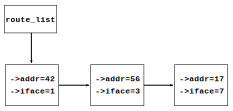
\includegraphics{defer/RouteList}}
\end{center}
\caption{Pre-BSD Packet Routing List}
\label{fig:defer:Pre-BSD Packet Routing List}
\end{figure}

{ \scriptsize
\begin{verbbox}
 1 struct route_entry {
 2   struct cds_list_head re_next;
 3   unsigned long addr;
 4   unsigned long iface;
 5 };
 6 CDS_LIST_HEAD(route_list);
 7
 8 unsigned long route_lookup(unsigned long addr)
 9 {
10   struct route_entry *rep;
11   unsigned long ret;
12
13   cds_list_for_each_entry(rep,
14                           &route_list, re_next) {
15     if (rep->addr == addr) {
16       ret = rep->iface;
17       return ret;
18     }
19   }
20   return ULONG_MAX;
21 }
22
23 int route_add(unsigned long addr,
24               unsigned long interface)
25 {
26   struct route_entry *rep;
27
28   rep = malloc(sizeof(*rep));
29   if (!rep)
30     return -ENOMEM;
31   rep->addr = addr;
32   rep->iface = interface;
33   cds_list_add(&rep->re_next, &route_list);
34   return 0;
35 }
36
37 int route_del(unsigned long addr)
38 {
39   struct route_entry *rep;
40
41   cds_list_for_each_entry(rep,
42                           &route_list, re_next) {
43     if (rep->addr == addr) {
44       cds_list_del(&rep->re_next);
45       free(rep);
46       return 0;
47     }
48   }
49   return -ENOENT;
50 }
\end{verbbox}
}
\begin{figure}[bp]
\centering
\theverbbox
\caption{Sequential Pre-BSD Routing Table}
\label{fig:defer:Sequential Pre-BSD Routing Table}
\end{figure}

Figure~\ref{fig:defer:Sequential Pre-BSD Routing Table}
shows a simple single-threaded implementation corresponding to
Figure~\ref{fig:defer:Pre-BSD Packet Routing List}.
Lines~1-5 define a \co{route_entry} structure and line~6 defines
the \co{route_list} header.
Lines~8-21 define \co{route_lookup()}, which sequentially searches
\co{route_list}, returning the corresponding \co{->iface}, or
\co{ULONG_MAX} if there is no such route entry.
Lines~23-35 define \co{route_add()}, which allocates a
\co{route_entry} structure, initializes it, and adds it to the
list, returning \co{-ENOMEM} in case of memory-allocation failure.
Finally, lines~37-50 define \co{route_del()}, which removes and
frees the specified \co{route_entry} structure if it exists,
or returns \co{-ENOENT} otherwise.

This single-threaded implementation serves as a prototype for the various
concurrent implementations in this chapter, and also as an estimate of
ideal scalability and performance.

% defer/refcnt.tex

\section{Reference Counting}
\label{sec:defer:Reference Counting}

Reference counting tracks the number of references
to a given object in order to prevent that object from being prematurely
freed.
Although this is a conceptually simple technique, many devils hide in
the details.
After all, if the object was not subject to being prematurely freed,
there would be no need for the reference counter.
But if the object \emph{is} subject to being prematurely freed,
what prevents that object from being freed during
the reference-acquisition process itself?

There are a number of possible answers to this question, including:

\begin{enumerate}
\item	A lock residing outside of the object must be held while
	manipulating the reference count.
	Note that there are a wide variety of types of locks,
	however, pretty much any type will suffice.
\item	The object is created with a non-zero reference count, and new
	references may be acquired only when the current value of
	the reference counter is non-zero.
	Once acquired, a reference may be handed off to some
	other entity.
\item	An existence guarantee is provided for the object, so that
	it cannot be freed during any time interval when some
	entity might be attempting to acquire a reference.
	Existence guarantees are often provided by automatic
	garbage collectors, and, as will be seen in
	Section~\ref{sec:defer:Read-Copy Update (RCU)}, they can
	also be provided by RCU.
\item	A type-safety guarantee is provided for the object, and there
	is in addition some identity check that can be performed once
	the reference is acquired.
	Type-safety guarantees can be provided by special-purpose
	memory allocators, and can also be provided by the
	\url{SLAB_DESTROY_BY_RCU} feature within the Linux kernel,
	again, as will be seen in
	Section~\ref{sec:defer:Read-Copy Update (RCU)}.
\end{enumerate}

Of course, any mechanism that provides existence guarantees
by definition also provides type-safety guarantees.
This section will therefore group the last two answers together under the
rubric of RCU, leaving us with three general categories of
reference-acquisition protection, namely, locking, reference counting,
and RCU.

\QuickQuiz{}
	Why not implement reference-acquisition using
	a simple compare-and-swap operation that only
	acquires a reference if the reference counter is
	non-zero?
\QuickQuizAnswer{
	Although this can resolve the race between the release of
	the last reference and acquisition of a new reference,
	it does absolutely nothing to prevent the data structure
	from being freed and reallocated, possibly as some completely
	different type of structure.
	It is quite likely that the ``simple compare-and-swap
	operation'' would give undefined results if applied to the
	differently typed structure.

	In short, use of atomic operations such as compare-and-swap
	absolutely requires either type-safety or existence guarantees.
} \QuickQuizEnd

\begin{table}
\centering
\begin{tabular}{l||c|c|c}
	& \multicolumn{3}{c}{Release Synchronization} \\
	\cline{2-4}
	Acquisition     &         & Reference &     \\
	Synchronization & Locking & Counting  & RCU \\
	\hline
	\hline
	Locking		& -	  & CAM	      & CA  \\
	\hline
	Reference	& A	  & AM	      & A   \\
	Counting	&  	  &   	      &     \\
	\hline
	RCU		& CA	  & MCA	      & CA  \\
\end{tabular}
\caption{Reference Counting and Synchronization Mechanisms}
\label{tab:defer:Reference Counting and Synchronization Mechanisms}
\end{table}

Given that the key reference-counting issue
is synchronization between acquisition
of a reference and freeing of the object, we have nine possible
combinations of mechanisms, as shown in
Table~\ref{tab:defer:Reference Counting and Synchronization Mechanisms}.
This table
divides reference-counting mechanisms into the following broad categories:
\begin{enumerate}
\item	Simple counting with neither atomic operations, memory
	barriers, nor alignment constraints \makebox{(``-'')}.
\item	Atomic counting without memory barriers (``A'').
\item	Atomic counting, with memory barriers required only on release
	(``AM'').
\item	Atomic counting with a check combined with the atomic acquisition
	operation, and with memory barriers required only on release
	(``CAM'').
\item	Atomic counting with a check combined with the atomic acquisition
	operation (``CA'').
\item	Atomic counting with a check combined with the atomic acquisition
	operation, and with memory barriers also required on acquisition
	(``MCA'').
\end{enumerate}
However, because all Linux-kernel atomic operations that return a
value are defined to contain memory barriers, all release operations
contain memory barriers, and all checked acquisition operations also
contain memory barriers.
Therefore, cases ``CA'' and ``MCA'' are equivalent to ``CAM'', so that
there are sections below for only the first four cases:
\makebox{``-''}, ``A'', ``AM'', and ``CAM''.
The Linux primitives that support reference counting are presented in
Section~\ref{sec:defer:Linux Primitives Supporting Reference Counting}.
Later sections cite optimizations that can improve performance
if reference acquisition and release is very frequent, and the
reference count need be checked for zero only very rarely.

\subsection{Implementation of Reference-Counting Categories}
\label{sec:defer:Implementation of Reference-Counting Categories}

Simple counting protected by locking (\makebox{``-''}) is described in
Section~\ref{sec:defer:Simple Counting},
atomic counting with no memory barriers (``A'') is described in
Section~\ref{sec:defer:Atomic Counting}
atomic counting with acquisition memory barrier (``AM'') is described in
Section~\ref{sec:defer:Atomic Counting With Release Memory Barrier},
and
atomic counting with check and release memory barrier (``CAM'') is described in
Section~\ref{sec:defer:Atomic Counting With Check and Release Memory Barrier}.

\subsubsection{Simple Counting}
\label{sec:defer:Simple Counting}

Simple counting, with neither atomic operations nor memory barriers,
can be used when the reference-counter acquisition and release are
both protected by the same lock.
In this case, it should be clear that the reference count itself
may be manipulated non-atomically, because the lock provides any
necessary exclusion, memory barriers, atomic instructions, and disabling
of compiler optimizations.
This is the method of choice when the lock is required to protect
other operations in addition to the reference count, but where
a reference to the object must be held after the lock is released.
Figure~\ref{fig:defer:Simple Reference-Count API} shows a simple
API that might be used to implement simple non-atomic reference
counting -- although simple reference counting is almost always
open-coded instead.

\begin{figure}[htbp]
{ \scriptsize
\begin{verbatim}
  1 struct sref {
  2   int refcount;
  3 };
  4
  5 void sref_init(struct sref *sref)
  6 {
  7   sref->refcount = 1;
  8 }
  9
 10 void sref_get(struct sref *sref)
 11 {
 12   sref->refcount++;
 13 }
 14
 15 int sref_put(struct sref *sref,
 16              void (*release)(struct sref *sref))
 17 {
 18   WARN_ON(release == NULL);
 19   WARN_ON(release == (void (*)(struct sref *))kfree);
 20
 21   if (--sref->refcount == 0) {
 22     release(sref);
 23     return 1;
 24   }
 25   return 0;
 26 }
\end{verbatim}
}
\caption{Simple Reference-Count API}
\label{fig:defer:Simple Reference-Count API}
\end{figure}

\subsubsection{Atomic Counting}
\label{sec:defer:Atomic Counting}

Simple atomic counting may be used in cases where any CPU acquiring
a reference must already hold a reference.
This style is used when a single CPU creates an object for its
own private use, but must allow other CPU, tasks, timer handlers,
or I/O completion handlers that it later spawns to also access this object.
Any CPU that hands the object off must first acquire a new reference
on behalf of the recipient object.
In the Linux kernel, the \url{kref} primitives are used to implement
this style of reference counting, as shown in
Figure~\ref{fig:defer:Linux Kernel kref API}.

Atomic counting is required
because locking is not used to protect all reference-count operations,
which means that it is possible for two different CPUs to concurrently
manipulate the reference count.
If normal increment and decrement were used, a pair of CPUs might both
fetch the reference count concurrently, perhaps both obtaining
the value ``3''.
If both of them increment their value, they will both obtain ``4'',
and both will store this value back into the counter.
Since the new value of the counter should instead be ``5'', one
of the two increments has been lost.
Therefore, atomic operations must be used both for counter increments
and for counter decrements.

If releases are guarded by locking or RCU,
memory barriers are \emph{not} required, but for different reasons.
In the case of locking, the locks provide any needed memory barriers
(and disabling of compiler optimizations), and the locks also
prevent a pair of releases from running concurrently.
In the case of RCU, cleanup must be deferred until all currently
executing RCU read-side critical sections have completed, and
any needed memory barriers or disabling of compiler optimizations
will be provided by the RCU infrastructure.
Therefore, if two CPUs release the final two references concurrently,
the actual cleanup will be deferred until both CPUs exit their
RCU read-side critical sections.

\QuickQuiz{}
	Why isn't it necessary to guard against cases where one CPU
	acquires a reference just after another CPU releases the last
	reference?
\QuickQuizAnswer{
	Because a CPU must already hold a reference in order
	to legally acquire another reference.
	Therefore, if one CPU releases the last reference,
	there cannot possibly be any CPU that is permitted
	to acquire a new reference.
	This same fact allows the non-atomic check in line~22
	of Figure~\ref{fig:defer:Linux Kernel kref API}.
} \QuickQuizEnd

\begin{figure}[htbp]
{ \scriptsize
\begin{verbatim}
  1 struct kref {
  2   atomic_t refcount;
  3 };
  4
  5 void kref_init(struct kref *kref)
  6 {
  7   atomic_set(&kref->refcount,1);
  8 }
  9
 10 void kref_get(struct kref *kref)
 11 {
 12   WARN_ON(!atomic_read(&kref->refcount));
 13   atomic_inc(&kref->refcount);
 14 }
 15
 16 int kref_put(struct kref *kref,
 17              void (*release)(struct kref *kref))
 18 {
 19   WARN_ON(release == NULL);
 20   WARN_ON(release == (void (*)(struct kref *))kfree);
 21
 22   if ((atomic_read(&kref->refcount) == 1) ||
 23       (atomic_dec_and_test(&kref->refcount))) {
 24     release(kref);
 25     return 1;
 26   }
 27   return 0;
 28 }
\end{verbatim}
}
\caption{Linux Kernel kref API}
\label{fig:defer:Linux Kernel kref API}
\end{figure}

The \url{kref} structure itself, consisting of a single atomic
data item, is shown in lines~1-3 of
Figure~\ref{fig:defer:Linux Kernel kref API}.
The \url{kref_init()} function on lines~5-8 initializes the counter
to the value ``1''.
Note that the \url{atomic_set()} primitive is a simple
assignment, the name stems from the data type of \url{atomic_t}
rather than from the operation.
The \url{kref_init()} function must be invoked during object creation,
before the object has been made available to any other CPU.

The \url{kref_get()} function on lines~10-14 unconditionally atomically
increments the counter.
The \url{atomic_inc()} primitive does not necessarily explicitly
disable compiler
optimizations on all platforms, but the fact that the \url{kref}
primitives are in a separate module and that the Linux kernel build
process does no cross-module optimizations has the same effect.

The \url{kref_put()} function on lines~16-28 checks for the counter having the
value ``1'' on line~22
(in which case no concurrent \url{kref_get()} is permitted),
or if atomically decrementing the counter results in zero on line~23.
In either of these two cases, \url{kref_put()} invokes the
specified \url{release} function and returns ``1'', telling the
caller that cleanup was performed.
Otherwise, \url{kref_put()} returns ``0''.

\QuickQuiz{}
	If the check on line~22 of
	Figure~\ref{fig:defer:Linux Kernel kref API} fails, how
	could the check on line~23 possibly succeed?
\QuickQuizAnswer{
	Suppose that {\tt kref\_put()} is protected by RCU, so
	that two CPUs might be executing line~22 concurrently.
	Both might see the value ``2'', causing both to then
	execute line~23.
	One of the two instances of {\tt atomic\_dec\_and\_test()}
	will decrement the value to zero and thus return 1.
} \QuickQuizEnd

\QuickQuiz{}
	How can it possibly be safe to non-atomically check for equality
	with ``1'' on line~22 of
	Figure~\ref{fig:defer:Linux Kernel kref API}?
\QuickQuizAnswer{
	Remember that it is not legal to call either {\tt kref\_get()}
	or {\tt kref\_put()} unless you hold a reference.
	If the reference count is equal to ``1'', then there
	can't possibly be another CPU authorized to change the
	value of the reference count.
} \QuickQuizEnd

\subsubsection{Atomic Counting With Release Memory Barrier}
\label{sec:defer:Atomic Counting With Release Memory Barrier}

This style of reference is used in the Linux kernel's networking
layer to track the destination caches that are used in packet routing.
The actual implementation is quite a bit more involved; this section
focuses on the aspects of \url{struct} \url{dst_entry} reference-count
handling that matches this use case,
shown in Figure~\ref{fig:defer:Linux Kernel dst-clone API}.

\begin{figure}[htbp]
{ \scriptsize
\begin{verbatim}
  1 static inline
  2 struct dst_entry * dst_clone(struct dst_entry * dst)
  3 {
  4   if (dst)
  5     atomic_inc(&dst->__refcnt);
  6   return dst;
  7 }
  8
  9 static inline
 10 void dst_release(struct dst_entry * dst)
 11 {
 12   if (dst) {
 13     WARN_ON(atomic_read(&dst->__refcnt) < 1);
 14     smp_mb__before_atomic_dec();
 15     atomic_dec(&dst->__refcnt);
 16   }
 17 }
\end{verbatim}
}
\caption{Linux Kernel dst\_clone API}
\label{fig:defer:Linux Kernel dst-clone API}
\end{figure}

The \url{dst_clone()} primitive may be used if the caller
already has a reference to the specified \url{dst_entry},
in which case it obtains another reference that may be handed off
to some other entity within the kernel.
Because a reference is already held by the caller, \url{dst_clone()}
need not execute any memory barriers.
The act of handing the \url{dst_entry} to some other entity might
or might not require a memory barrier, but if such a memory barrier
is required, it will be embedded in the mechanism used to hand the
\url{dst_entry} off.

The \url{dst_release()} primitive may be invoked from any environment,
and the caller might well reference elements of the \url{dst_entry}
structure immediately prior to the call to \url{dst_release()}.
The \url{dst_release()} primitive therefore contains a memory
barrier on line~14 preventing both the compiler and the CPU
from misordering accesses.

Please note that the programmer making use of \url{dst_clone()} and
\url{dst_release()} need not be aware of the memory barriers, only
of the rules for using these two primitives.

\subsubsection{Atomic Counting With Check and Release Memory Barrier}
\label{sec:defer:Atomic Counting With Check and Release Memory Barrier}

The fact that reference-count acquisition can run concurrently
with reference-count release adds further complications.
Suppose that a reference-count release finds that the new
value of the reference count is zero, signalling that it is
now safe to clean up the reference-counted object.
We clearly cannot allow a reference-count acquisition to
start after such clean-up has commenced, so the acquisition
must include a check for a zero reference count.
This check must be part of the atomic increment operation,
as shown below.

\QuickQuiz{}
	Why can't the check for a zero reference count be
	made in a simple ``if'' statement with an atomic
	increment in its ``then'' clause?
\QuickQuizAnswer{
	Suppose that the ``if'' condition completed, finding
	the reference counter value equal to one.
	Suppose that a release operation executes, decrementing
	the reference counter to zero and therefore starting
	cleanup operations.
	But now the ``then'' clause can increment the counter
	back to a value of one, allowing the object to be
	used after it has been cleaned up.
} \QuickQuizEnd

The Linux kernel's \url{fget()} and \url{fput()} primitives
use this style of reference counting.
Simplified versions of these functions are shown in
Figure~\ref{fig:defer:Linux Kernel fget/fput API}.

\begin{figure}[htbp]
{ \scriptsize
\begin{verbatim}
  1 struct file *fget(unsigned int fd)
  2 {
  3   struct file *file;
  4   struct files_struct *files = current->files;
  5
  6   rcu_read_lock();
  7   file = fcheck_files(files, fd);
  8   if (file) {
  9     if (!atomic_inc_not_zero(&file->f_count)) {
 10       rcu_read_unlock();
 11       return NULL;
 12     }
 13   }
 14   rcu_read_unlock();
 15   return file;
 16 }
 17
 18 struct file *
 19 fcheck_files(struct files_struct *files, unsigned int fd)
 20 {
 21   struct file * file = NULL;
 22   struct fdtable *fdt = rcu_dereference((files)->fdt);
 23
 24   if (fd < fdt->max_fds)
 25     file = rcu_dereference(fdt->fd[fd]);
 26   return file;
 27 }
 28
 29 void fput(struct file *file)
 30 {
 31   if (atomic_dec_and_test(&file->f_count))
 32     call_rcu(&file->f_u.fu_rcuhead, file_free_rcu);
 33 }
 34
 35 static void file_free_rcu(struct rcu_head *head)
 36 {
 37   struct file *f;
 38
 39   f = container_of(head, struct file, f_u.fu_rcuhead);
 40   kmem_cache_free(filp_cachep, f);
 41 }
\end{verbatim}
}
\caption{Linux Kernel fget/fput API}
\label{fig:defer:Linux Kernel fget/fput API}
\end{figure}

Line~4 of \url{fget()} fetches the a pointer to the current
process's file-descriptor table, which might well be shared
with other processes.
Line~6 invokes \url{rcu_read_lock()}, which
enters an RCU read-side critical section.
The callback function from any subsequent \url{call_rcu()} primitive
will be deferred until a matching \url{rcu_read_unlock()} is reached
(line~10 or 14 in this example).
Line~7 looks up the file structure corresponding to the file
descriptor specified by the \url{fd} argument, as will be
described later.
If there is an open file corresponding to the specified file descriptor,
then line~9 attempts to atomically acquire a reference count.
If it fails to do so, lines~10-11 exit the RCU read-side critical
section and report failure.
Otherwise, if the attempt is successful, lines~14-15 exit the read-side
critical section and return a pointer to the file structure.

The \url{fcheck_files()} primitive is a helper function for
\url{fget()}.
It uses the \url{rcu_dereference()} primitive to safely fetch an
RCU-protected pointer for later dereferencing (this emits a
memory barrier on CPUs such as DEC Alpha in which data dependencies
do not enforce memory ordering).
Line~22 uses \url{rcu_dereference()} to fetch a pointer to this
task's current file-descriptor table,
and line~24 checks to see if the specified file descriptor is in range.
If so, line~25 fetches the pointer to the file structure, again using
the \url{rcu_dereference()} primitive.
Line~26 then returns a pointer to the file structure or \url{NULL}
in case of failure.

The \url{fput()} primitive releases a reference to a file structure.
Line~31 atomically decrements the reference count, and, if the result
was zero, line~32 invokes the \url{call_rcu()} primitives in order to
free up the file structure (via the \url{file_free_rcu()} function
specified in \url{call_rcu()}'s second argument),
but only after all currently-executing
RCU read-side critical sections complete.
The time period required for all currently-executing RCU read-side
critical sections to complete is termed a ``grace period''.
Note that the \url{atomic_dec_and_test()} primitive contains
a memory barrier.
This memory barrier is not necessary in this example, since the structure
cannot be destroyed until the RCU read-side critical section completes,
but in Linux, all atomic operations that return a result must
by definition contain memory barriers.

Once the grace period completes, the \url{file_free_rcu()} function
obtains a pointer to the file structure on line~39, and frees it
on line~40.

This approach is also used by Linux's virtual-memory system,
see \url{get_page_unless_zero()} and \url{put_page_testzero()} for
page structures as well as \url{try_to_unuse()} and \url{mmput()}
for memory-map structures.

\subsection{Linux Primitives Supporting Reference Counting}
\label{sec:defer:Linux Primitives Supporting Reference Counting}

The Linux-kernel primitives used in the above examples are
summarized in the following list.
\IfInBook{}{The RCU primitives may be unfamiliar to some readers,
	    so a brief overview with citations is included in
	    Section~\ref{sec:defer:Background on RCU}.}

\begin{itemize}
\item	{\tt atomic\_t}~~
	Type definition for 32-bit quantity to be manipulated atomically.
\item	{\tt void atomic\_dec(atomic\_t *var);}~~
	Atomically decrements the referenced variable without necessarily
	issuing a memory barrier or disabling compiler optimizations.
\item	{\tt int atomic\_dec\_and\_test(atomic\_t *var);}~~
	Atomically decrements the referenced variable, returning
	TRUE if the result is zero.
	Issues a memory barrier and disables compiler optimizations that
	might otherwise move memory references across this primitive.
\item	{\tt void atomic\_inc(atomic\_t *var);}~~
	Atomically increments the referenced variable without necessarily
	issuing a memory barrier or disabling compiler optimizations.
\item	{\tt int atomic\_inc\_not\_zero(atomic\_t *var);}~~
	Atomically increments the referenced variable, but only if the
	value is non-zero, and returning TRUE if the increment occurred.
	Issues a memory barrier and disables compiler optimizations that
	might otherwise move memory references across this primitive.
\item	{\tt int atomic\_read(atomic\_t *var);}~~
	Returns the integer value of the referenced variable.
	This is not an atomic operation, and it neither issues memory
	barriers nor disables compiler optimizations.
\item	{\tt void atomic\_set(atomic\_t *var, int val);}~~
	Sets the value of the referenced atomic variable to ``val''.
	This is not an atomic operation, and it neither issues memory
	barriers nor disables compiler optimizations.
\item	{\tt void call\_rcu(struct rcu\_head *head, void (*func)(struct rcu\_head *head));}~~
	Invokes \url{func(head)} some time after all currently executing RCU
	read-side critical sections complete, however, the \url{call_rcu()}
	primitive returns immediately.
	Note that \url{head} is normally a field within an RCU-protected
	data structure, and that \url{func} is normally a function that
	frees up this data structure.
	The time interval between the invocation of \url{call_rcu()} and
	the invocation of \url{func} is termed a ``grace period''.
	Any interval of time containing a grace period is itself a
	grace period.
\item	{\tt type *container\_of(p, type, f);}~~
	Given a pointer ``p'' to a field ``f'' within a structure
	of the specified type, return a pointer to the structure.
\item	{\tt void rcu\_read\_lock(void);}~~
	Marks the beginning of an RCU read-side critical section.
\item	{\tt void rcu\_read\_unlock(void);}~~
	Marks the end of an RCU read-side critical section.
	RCU read-side critical sections may be nested.
\item	{\tt void smp\_mb\_\_before\_atomic\_dec(void);}~~
	Issues a memory barrier and disables code-motion compiler
	optimizations only if the platform's \url{atomic_dec()}
	primitive does not already do so.
\item	{\tt struct rcu\_head}~~
	A data structure used by the RCU infrastructure to track
	objects awaiting a grace period.
	This is normally included as a field within an RCU-protected
	data structure.
\end{itemize}

\subsection{Counter Optimizations}
\label{sec:defer:Counter Optimizations}

In some cases where increments and decrements are common, but checks
for zero are rare, it makes sense to maintain per-CPU or per-task
counter.
\IfInBook{See Appendix~\ref{app:rcuimpl:Sleepable RCU Implementation}
	  for an example of this technique.}{
	  See the paper on sleepable read-copy update
	  (SRCU) for an example of this technique~\cite{PaulEMcKenney2006c}.}
% @@@ need a section or chapter on counting...
This approach eliminates the need for atomic instructions or memory
barriers on the increment and decrement primitives, but still requires
that code-motion compiler optimizations be disabled.
In addition, the primitives such as \url{synchronize_srcu()}
that check for the aggregate reference
count reaching zero can be quite slow.
This underscores the fact that these techniques are designed
for situations where the references are frequently acquired and
released, but where it is rarely necessary to check for a zero
reference count.

% defer/hazptr.tex
% Can I hazptr cheezeberger?

\section{Hazard Pointers}
\label{sec:defer:Hazard Pointers}

One way of avoiding problems with concurrent reference counting
is to implement the reference counters
inside out, that is, rather than incrementing an integer stored in the
data element, instead store a pointer to that data element in
per-CPU (or per-thread) lists.
Each element of these lists is called a
\emph{hazard pointer}~\cite{MagedMichael04a}.\footnote{
	Also independently invented by others~\cite{HerlihyLM02}.}
The value of a given data element's ``virtual reference counter'' can
then be obtained by counting the number of hazard pointers referencing
that element.
Therefore, if that element has been rendered inaccessible to readers,
and there are no longer any hazard pointers referencing it, that element
may safely be freed.

{ \scriptsize
\begin{verbbox}
 1 int hp_store(void **p, void **hp)
 2 {
 3   void *tmp;
 4 
 5   tmp = ACCESS_ONCE(*p);
 6   ACCESS_ONCE(*hp) = tmp;
 7   smp_mb();
 8   if (tmp != ACCESS_ONCE(*p) ||
 9       tmp == HAZPTR_POISON) {
10     ACCESS_ONCE(*hp) = NULL;
11     return 0;
12   }
13   return 1;
14 }
15 
16 void hp_erase(void **hp)
17 {
18   smp_mb();
19   ACCESS_ONCE(*hp) = NULL;
20   hp_free(hp);
21 }
\end{verbbox}
}
\begin{figure}[btp]
\centering
\theverbbox
\caption{Hazard-Pointer Storage and Erasure}
\label{fig:defer:Hazard-Pointer Storage and Erasure}
\end{figure}

Of course, this means that hazard-pointer acquisition must be carried
out quite carefully in order to avoid destructive races with concurrent
deletion.
One implementation is shown in
Figure~\ref{fig:defer:Hazard-Pointer Storage and Erasure},
which shows \co{hp_store()} on lines~1-13 and \co{hp_erase()} on
lines~15-20.
The \co{smp_mb()} primitive will be described in detail in
Section~\ref{sec:advsync:Memory Barriers}, but may be ignored for
the purposes of this brief overview.

The \co{hp_store()} function records a hazard pointer at \co{hp} for the data
element whose pointer is referenced by \co{p}, while checking for
concurrent modifications.
If a concurrent modification occurred, \co{hp_store()} refuses to record
a hazard pointer, and returns zero to indicate that the caller must
restart its traversal from the beginning.
Otherwise, \co{hp_store()} returns one to indicate that it successfully
recorded a hazard pointer for the data element.

\QuickQuiz{}
	Why does \co{hp_store()} in
	Figure~\ref{fig:defer:Hazard-Pointer Storage and Erasure}
	take a double indirection to the data element?
	Why not \co{void *} instead of \co{void **}?
\QuickQuizAnswer{
	Because \co{hp_record()} must check for concurrent modifications.
	To do that job, it needs a pointer to a pointer to the element,
	so that it can check for a modification to the pointer to the
	element.
} \QuickQuizEnd

\QuickQuiz{}
	Why does \co{hp_store()}'s caller need to restart its
	traversal from the beginning in case of failure?
	Isn't that inefficient for large data structures?
\QuickQuizAnswer{
	It might be inefficient in some sense, but the fact is that
	such restarting is absolutely required for correctness.
	To see this, consider a hazard-pointer-protected linked list
	containing elements~A, B, and~C that is subjecte to the
	following sequence of events:

	\begin{enumerate}
	\item	Thread~0 stores a hazard pointer to element~B
		(having presumably traversed to element~B from element~A).
	\item	Thread~1 removes element~B from the list, which sets
		the pointer from element~B to element~C to a special
		\co{HAZPTR_POISON} value in order to mark the deletion.
		Because Thread~0 has a hazard pointer to element~B,
		it cannot yet be freed.
	\item	Thread~1 removes element~C from the list.
		Because there are no hazard pointers referencing element~C,
		it is immediately freed.
	\item	Thread~0 attempts to acquire a hazard pointer to
		now-removed element~B's successor, but sees the
		\co{HAZPTR_POISON} value, and thus returns zero,
		forcing the caller to restart its traversal from the
		beginning of the list.
	\end{enumerate}

	Which is a very good thing, because otherwise Thread~0 would
	have attempted to access the now-freed element~C,
	which might have resulted in arbitrarily horrible
	memory corruption, especially if the memory for
	element~C had since been re-allocated for some other
	purpose.

	All that aside, please understand that hazard pointers's
	restarting allows it to maintain a minimal memory footprint.
	Any object not currently referenced by some hazard pointer
	may be immediately freed.
	In contrast,
	Section~\ref{sec:defer:Read-Copy Update (RCU)}
	will discuss a mechanism that avoids read-side retries
	(and minimizes read-side overhead), but has a much larger
	memory footprint.
} \QuickQuizEnd

\QuickQuiz{}
	Given that papers on hazard pointers use the bottom bits
	of each pointer to mark deleted elements, what is up with
	\co{HAZPTR_POISON}?
\QuickQuizAnswer{
	The published implementations of hazard pointers used
	non-blocking synchronization techniques for insertion
	and deletion.
	These techniques require that readers traversing the
	data structure ``help'' updaters complete their updates,
	which in turn means that readers need to look at the successor
	of a deleted element.

	In contrast, we will be using locking to synchronize updates,
	which does away with the need for readers to help updaters
	complete their updates, which in turn allows us to leave
	pointers' bottom bits alone.
	This approach allows read-side code to be simpler and faster.
} \QuickQuizEnd

Because algorithms using hazard pointers might be restarted at any
step of their traversal through the data structure, such algorithms
must typically take care to avoid making any changes to the data
structure until after they have acquired all relevant hazard pointers.

\QuickQuiz{}
	But don't these restrictions on hazard pointers also apply
	to other forms of reference counting?
\QuickQuizAnswer{
	These restrictions apply only to reference-counting mechanisms whose
	reference acquisition can fail.
} \QuickQuizEnd

These restrictions result in great benefits to readers, courtesy of the
fact that the hazard pointers are stored local to each CPU/thread,
which in turn allows traversals of the data structures themselves to
be carried out in a completely read-only fashion.
Referring back to
Figure~\ref{fig:count:Optimization and the Four Parallel-Programming Tasks}
on
page~\pageref{fig:count:Optimization and the Four Parallel-Programming Tasks},
hazard pointers enable the CPU caches to do resource replication, which
in turn allows weakening of the parallel-access-control mechanism,
thus boosting performance and scalability.
Performance comparisons with other mechanisms may be found in
Chapter~\ref{chp:Data Structures}
and in other publications~\cite{ThomasEHart2007a,McKenney:2013:SDS:2483852.2483867,MagedMichael04a}.

{ \scriptsize
\begin{verbbox}
 1 struct route_entry {
 2   struct hazptr_head hh;
 3   struct route_entry *re_next;
 4   unsigned long addr;
 5   unsigned long iface;
 6   int re_freed;
 7 };
 8 struct route_entry route_list;
 9 DEFINE_SPINLOCK(routelock);
10 hazard_pointer __thread *my_hazptr;
11
12 unsigned long route_lookup(unsigned long addr)
13 {
14   int offset = 0;
15   struct route_entry *rep;
16   struct route_entry **repp;
17
18 retry:
19   repp = &route_list.re_next;
20   do {
21     rep = ACCESS_ONCE(*repp);
22     if (rep == NULL)
23       return ULONG_MAX;
24     if (rep == (struct route_entry *)HAZPTR_POISON)
25       goto retry;
26     my_hazptr[offset].p = &rep->hh;
27     offset = !offset;
28     smp_mb();
29     if (ACCESS_ONCE(*repp) != rep)
30       goto retry;
31     repp = &rep->re_next;
32   } while (rep->addr != addr);
33   if (ACCESS_ONCE(rep->re_freed))
34     abort();
35   return rep->iface;
36 }
\end{verbbox}
}
\begin{figure}[tbp]
\centering
\theverbbox
\caption{Hazard-Pointer Pre-BSD Routing Table Lookup}
\label{fig:defer:Hazard-Pointer Pre-BSD Routing Table Lookup}
\end{figure}

{ \scriptsize
\begin{verbbox}
 1 int route_add(unsigned long addr,
 2               unsigned long interface)
 3 {
 4   struct route_entry *rep;
 5
 6   rep = malloc(sizeof(*rep));
 7   if (!rep)
 8     return -ENOMEM;
 9   rep->addr = addr;
10   rep->iface = interface;
11   rep->re_freed = 0;
12   spin_lock(&routelock);
13   rep->re_next = route_list.re_next;
14   route_list.re_next = rep;
15   spin_unlock(&routelock);
16   return 0;
17 }
18
19 int route_del(unsigned long addr)
20 {
21   struct route_entry *rep;
22   struct route_entry **repp;
23
24   spin_lock(&routelock);
25   repp = &route_list.re_next;
26   for (;;) {
27     rep = *repp;
28     if (rep == NULL)
29       break;
30     if (rep->addr == addr) {
31       *repp = rep->re_next;
32       rep->re_next =
33           (struct route_entry *)HAZPTR_POISON;
34       spin_unlock(&routelock);
35       hazptr_free_later(&rep->hh);
36       return 0;
37     }
38     repp = &rep->re_next;
39   }
40   spin_unlock(&routelock);
41   return -ENOENT;
42 }
\end{verbbox}
}
\begin{figure}[tbp]
\centering
\theverbbox
\caption{Hazard-Pointer Pre-BSD Routing Table Add/Delete}
\label{fig:defer:Hazard-Pointer Pre-BSD Routing Table Add/Delete}
\end{figure}

The Pre-BSD routing example can use hazard pointers as shown in
Figure~\ref{fig:defer:Hazard-Pointer Pre-BSD Routing Table Lookup}
for data structures and \co{route_lookup()}, and in
Figure~\ref{fig:defer:Hazard-Pointer Pre-BSD Routing Table Add/Delete}
for \co{route_add()} and \co{route_del()}
(\path{route_hazptr.c}).
As with reference counting, the hazard-pointers implementation
is quite similar to the sequential algorithm shown in
Figure~\ref{fig:defer:Sequential Pre-BSD Routing Table}
on
page~\pageref{fig:defer:Sequential Pre-BSD Routing Table},
so only differences will be discussed.

Starting with
Figure~\ref{fig:defer:Hazard-Pointer Pre-BSD Routing Table Lookup},
line~2 shows the \co{->hh} field used to queue objects pending
hazard-pointer free,
line~6 shows the \co{->re_freed} field used to detect use-after-free bugs,
and lines~24-30 attempt to acquire a hazard pointer, branching
to line~18's \co{retry} label on failure.

In
Figure~\ref{fig:defer:Hazard-Pointer Pre-BSD Routing Table Add/Delete},
line~11 initializes \co{->re_freed},
lines~32 and~33 poison the \co{->re_next} field of the newly removed
object, and
line~35 passes that object to the hazard pointers's
\co{hazptr_free_later()} function, which will free that object once it
is safe to do so.
The spinlocks work the same as in
Figure~\ref{fig:defer:Reference-Counted Pre-BSD Routing Table Add/Delete}.

\begin{figure}[tb]
\centering
\resizebox{2.5in}{!}{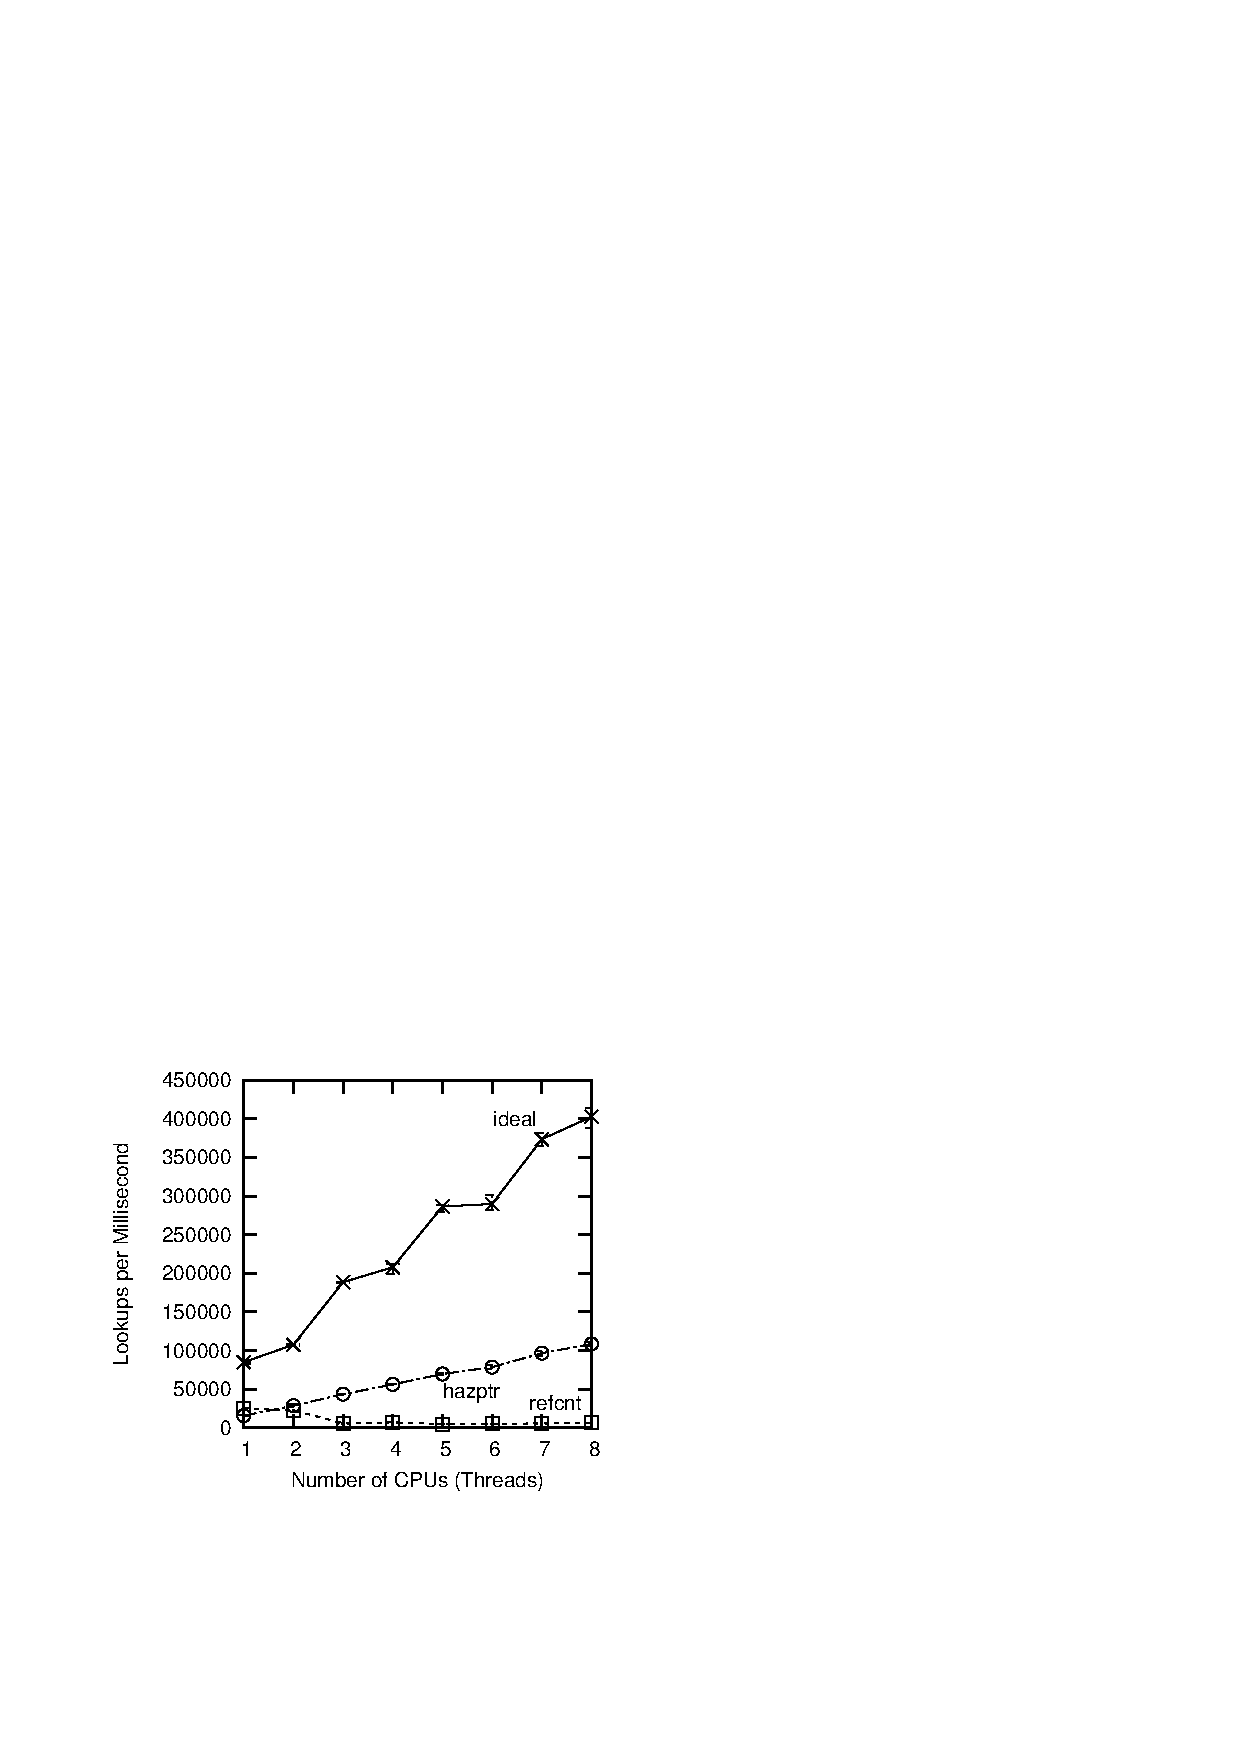
\includegraphics{CodeSamples/defer/perf-hazptr}}
\caption{Pre-BSD Routing Table Protected by Hazard Pointers}
\label{fig:defer:Pre-BSD Routing Table Protected by Hazard Pointers}
\end{figure}

Figure~\ref{fig:defer:Pre-BSD Routing Table Protected by Hazard Pointers}
shows the hazard-pointers-protected Pre-BSD routing algorithm's
performance on the same read-only workload as for
Figure~\ref{fig:defer:Pre-BSD Routing Table Protected by Reference Counting}.
Although hazard pointers scales much better than does reference counting,
hazard pointers still require readers to do writes to shared
memory (albeit with much improved locality of reference),
and also require a full memory barrier and retry check for each
object traversed.
Therefore, hazard pointers's performance is far short of ideal.
On the other hand, hazard pointers do operate correctly for workloads
involving concurrent updates.

\QuickQuiz{}
	The paper ``Structured Deferral: Synchronization via
	Procrastination''~\cite{McKenney:2013:SDS:2483852.2483867}
	shows that hazard pointers have near-ideal performance.
	Whatever happened in
	Figure~\ref{fig:defer:Pre-BSD Routing Table Protected by Hazard Pointers}???
\QuickQuizAnswer{
	First,
	Figure~\ref{fig:defer:Pre-BSD Routing Table Protected by Hazard Pointers}
	has a linear y-axis, while most of the graphs in the
	``Structured Deferral'' paper have logscale y-axes.
	Next, that paper uses hash tables, while
	Figure~\ref{fig:defer:Pre-BSD Routing Table Protected by Hazard Pointers}'s
	uses a simple linked list.
	Finally, that paper used a larger and older x86 system, while
	a newer but smaller system that was used to generate the data
	shown in
	Figure~\ref{fig:defer:Pre-BSD Routing Table Protected by Hazard Pointers}.
} \QuickQuizEnd

The next section attempts to improve on hazard pointers by using
sequence locks, which avoid both read-side writes and per-object memory
barriers.

% defer/seqlock.tex

\section{Sequence Locks}
\label{sec:defer:Sequence Locks}

\begin{figure}[tb]
\begin{center}
\resizebox{3in}{!}{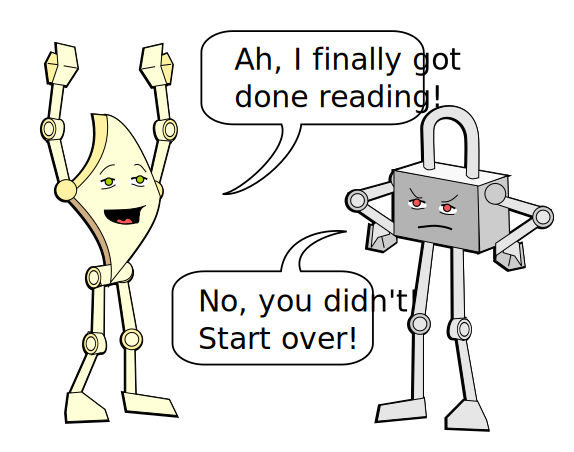
\includegraphics{cartoons/r-2014-Start-over}}
\end{center}
\caption{Reader And Uncooperative Sequence Lock}
\label{fig:defer:Reader And Uncooperative Sequence Lock}
\end{figure}

Sequence locks are used in the Linux kernel for read-mostly data that
must be seen in a consistent state by readers.
However, unlike reader-writer locking, readers do not exclude writers.
Instead, like hazard pointers, sequence locks force readers to
\emph{retry} an operation if they detect activity from a concurrent writer.
As can be seen from
Figure~\ref{fig:defer:Reader And Uncooperative Sequence Lock},
it is important to design code using sequence locks so that readers
very rarely need to retry.

\QuickQuiz{}
	Why isn't this sequence-lock discussion in Chapter~\ref{chp:Locking},
	you know, the one on \emph{locking}?
\QuickQuizAnswer{
	The sequence-lock mechanism is really a combination of two
	separate synchronization mechanisms, sequence counts and
	locking.
	In fact, the sequence-count mechanism is available separately
	in the Linux kernel via the
	\co{write_seqcount_begin()} and \co{write_seqcount_end()}
	primitives.

	However, the combined \co{write_seqlock()} and
	\co{write_sequnlock()} primitives are used much more heavily
	in the Linux kernel.
	More importantly, many more people will understand what you
	mean if you say ``sequence lock'' than if you say
	``sequence count''.

	So this section is entitled ``Sequence Locks'' so that people
	will understand what it is about just from the title, and
	it appears in the ``Deferred Processing'' because (1) of the
	emphasis on the ``sequence count'' aspect of ``sequence locks''
	and (2) because a ``sequence lock'' is much more than merely
	a lock.
} \QuickQuizEnd

{ \scriptsize
\begin{verbbox}
  1 do {
  2   seq = read_seqbegin(&test_seqlock);
  3   /* read-side access. */
  4 } while (read_seqretry(&test_seqlock, seq));
\end{verbbox}
}
\begin{figure}[bp]
\centering
\theverbbox
\caption{Sequence-Locking Reader}
\label{fig:defer:Sequence-Locking Reader}
\end{figure}

{ \scriptsize
\begin{verbbox}
  1 write_seqlock(&test_seqlock);
  2 /* Update */
  3 write_sequnlock(&test_seqlock);
\end{verbbox}
}
\begin{figure}[bp]
\centering
\theverbbox
\caption{Sequence-Locking Writer}
\label{fig:defer:Sequence-Locking Writer}
\end{figure}

The key component of sequence locking is the sequence number, which has
an even value in the absence of writers and an odd value if there
is an update in progress.
Readers can then snapshot the value before and after each access.
If either snapshot has an odd value, or if the two snapshots differ,
there has been a concurrent update, and the reader must discard
the results of the access and then retry it.
Readers use the \co{read_seqbegin()} and \co{read_seqretry()}
functions, as shown in Figure~\ref{fig:defer:Sequence-Locking Reader},
when accessing data protected by a sequence lock.
Writers must increment the value before and after each update,
and only one writer is permitted at a given time.
Writers use the \co{write_seqlock()} and \co{write_sequnlock()}
functions, as shown in Figure~\ref{fig:defer:Sequence-Locking Writer},
when updating data protected by a sequence lock.

Sequence-lock-protected data can have an arbitrarily large number of
concurrent readers, but only one writer at a time.
Sequence locking is used in the Linux kernel to protect calibration
quantities used for timekeeping.
It is also used in pathname traversal to detect concurrent rename operations.

\QuickQuiz{}
	Can you use sequence locks as the only synchronization
	mechanism protecting a linked list supporting concurrent
	addition, deletion, and search?
\QuickQuizAnswer{
	One trivial way of accomplishing this is to surround all
	accesses, including the read-only accesses, with
	\co{write_seqlock()} and \co{write_sequnlock()}.
	Of course, this solution also prohibits all read-side
	parallelism, and furthermore could just as easily be implemented
	using simple locking.

	If you do come up with a solution that uses \co{read_seqbegin()}
	and \co{read_seqretry()} to protect read-side accesses, make
	sure that you correctly handle the following sequence of events:

	\begin{enumerate}
	\item	CPU~0 is traversing the linked list, and picks up a pointer
		to list element~A.
	\item	CPU~1 removes element~A from the list and frees it.
	\item	CPU~2 allocates an unrelated data structure, and gets
		the memory formerly occupied by element~A.
		In this unrelated data structure, the memory previously
		used for element~A's \co{->next} pointer is now occupied
		by a floating-point number.
	\item	CPU~0 picks up what used to be element~A's \co{->next}
		pointer, gets random bits, and therefore gets a
		segmentation fault.
	\end{enumerate}

	One way to protect against this sort of problem requires use
	of ``type-safe memory'', which will be discussed in
	Section~\ref{sec:defer:RCU is a Way of Providing Type-Safe Memory}.
	But in that case, you would be using some other synchronization
	mechanism in addition to sequence locks!
} \QuickQuizEnd

{ \scriptsize
\begin{verbbox}
  1 typedef struct {
  2   unsigned long seq;
  3   spinlock_t lock;
  4 } seqlock_t;
  5 
  6 static void seqlock_init(seqlock_t *slp)
  7 {
  8   slp->seq = 0;
  9   spin_lock_init(&slp->lock);
 10 }
 11 
 12 static unsigned long read_seqbegin(seqlock_t *slp)
 13 {
 14   unsigned long s;
 15 
 16 repeat:
 17   s = ACCESS_ONCE(slp->seq);
 18   smp_mb();
 19   if (unlikely(s & 1))
 20     goto repeat;
 21   return s;
 22 }
 23 
 24 static int read_seqretry(seqlock_t *slp,
 25                          unsigned long oldseq)
 26 {
 27   unsigned long s;
 28 
 29   smp_mb();
 30   s = ACCESS_ONCE(slp->seq);
 31   return s != oldseq;
 32 }
 33 
 34 static void write_seqlock(seqlock_t *slp)
 35 {
 36   spin_lock(&slp->lock);
 37   ++slp->seq;
 38   smp_mb();
 39 }
 40 
 41 static void write_sequnlock(seqlock_t *slp)
 42 {
 43   smp_mb();
 44   ++slp->seq;
 45   spin_unlock(&slp->lock);
 46 }
\end{verbbox}
}
\begin{figure}[bp]
\centering
\theverbbox
\caption{Sequence-Locking Implementation}
\label{fig:defer:Sequence-Locking Implementation}
\end{figure}

A simple implementation of sequence locks is shown in
Figure~\ref{fig:defer:Sequence-Locking Implementation}
(\co{seqlock.h}).
The \co{seqlock_t} data structure is shown on lines~1-4, and contains
the sequence number along with a lock to serialize writers.
Lines~6-10 show \co{seqlock_init()}, which, as the name indicates,
initializes a \co{seqlock_t}.

Lines~12-22 show \co{read_seqbegin()}, which begins a sequence-lock
read-side critical section.
Line~17 takes a snapshot of the sequence counter, and line~18 orders
this snapshot operation before the caller's critical section.
Line~19 checks to see if the snapshot is odd, indicating that there
is a concurrent writer, and, if so, line~20 jumps back to the beginning.
Otherwise, line~21 returns the value of the snapshot, which the caller
will pass to a later call to \co{read_seqretry()}.

\QuickQuiz{}
	Why bother with the check on line~19 of
	\co{read_seqbegin()} in
	Figure~\ref{fig:defer:Sequence-Locking Implementation}?
	Given that a new writer could begin at any time, why not
	simply incorporate the check into line~31 of
	\co{read_seqretry()}?
\QuickQuizAnswer{
	That would be a legitimate implementation.
	However, it would not save anything to move the check down
	to \co{read_seqretry()}: There would be roughly the same number
	of instructions.
	Furthermore, the reader's accesses from its doomed read-side
	critical section could inflict overhead on the writer in
	the form of cache misses.
	We can avoid these cache misses by placing the check in
	\co{read_seqbegin()} as shown on line~19 of
	Figure~\ref{fig:defer:Sequence-Locking Implementation}.
} \QuickQuizEnd

Lines~24-32 show \co{read_seqretry()}, which returns true if there
were no writers present since the time of the corresponding
call to \co{read_seqbegin()}.
Line~29 orders the caller's prior critical section before line~30's
fetch of the new snapshot of the sequence counter.
Finally, line~31 checks that the sequence counter has not changed,
in other words, that there has been no writer, and returns true if so.

\QuickQuiz{}
	Why is the \co{smp_mb()} on line~29 of
	Figure~\ref{fig:defer:Sequence-Locking Implementation}
	needed?
\QuickQuizAnswer{
	If it was omitted, both the compiler and the CPU would be
	within their rights to move the critical section preceding
	the call to \co{read_seqretry()} down below this function.
	This would prevent the sequence lock from protecting the
	critical section.
	The \co{smp_mb()} primitive prevents such reordering.
} \QuickQuizEnd

\QuickQuiz{}
	Can't weaker memory barriers be used in the code in
	Figure~\ref{fig:defer:Sequence-Locking Implementation}?
\QuickQuizAnswer{
	In older versions of the Linux kernel, no.

	In very new versions of the Linux kernel, line~17 could use
	\co{smp_load_acquire()} instead of \co{ACCESS_ONCE()}, which
	in turn would allow the \co{smp_mb()} on line~18 to be dropped.
	Similarly, line~44 could use an \co{smp_store_release()}, for
	example, as follows: \\
	\co{smp_store_release(&slp->seq, ACCESS_ONCE(slp->seq) + 1);} \\
	This would allow the \co{smp_mb()} on line~43 to be dropped.
} \QuickQuizEnd

\QuickQuiz{}
	What prevents sequence-locking updaters from starving readers?
\QuickQuizAnswer{
	Nothing.
	This is one of the weaknesses of sequence locking, and as a
	result, you should use sequence locking only in read-mostly
	situations.
	Unless of course read-side starvation is acceptable in your
	situation, in which case, go wild with the sequence-locking updates!
} \QuickQuizEnd

Lines~34-39 show \co{write_seqlock()}, which simply acquires the lock,
increments the sequence number, and executes a memory barrier to ensure
that this increment is ordered before the caller's critical section.
Lines~41-46 show \co{write_sequnlock()}, which executes a memory barrier
to ensure that the caller's critical section is ordered before the
increment of the sequence number on line~44, then releases the lock.

\QuickQuiz{}
	What if something else serializes writers, so that the lock
	is not needed?
\QuickQuizAnswer{
	In this case, the \co{->lock} field could be omitted, as it
	is in \co{seqcount_t} in the Linux kernel.
} \QuickQuizEnd

\QuickQuiz{}
	Why isn't \co{seq} on line~2 of
	Figure~\ref{fig:defer:Sequence-Locking Implementation}
	\co{unsigned} rather than \co{unsigned long}?
	After all, if \co{unsigned} is good enough for the Linux
	kernel, shouldn't it be good enough for everyone?
\QuickQuizAnswer{
	Not at all.
	The Linux kernel has a number of special attributes that allow
	it to ignore the following sequence of events:
	\begin{enumerate}
	\item	Thread~0 executes \co{read_seqbegin()}, picking up
		\co{->seq} in line~17, noting that the value is even,
		and thus returning to the caller.
	\item	Thread~0 starts executing its read-side critical section,
		but is then preempted for a long time.
	\item	Other threads repeatedly invoke \co{write_seqlock()} and
		\co{write_sequnlock()}, until the value of \co{->seq}
		overflows back to the value that Thread~0 fetched.
	\item	Thread~0 resumes execution, completing its read-side
		critical section with inconsistent data.
	\item	Thread~0 invokes \co{read_seqretry()}, which incorrectly
		concludes that Thread~0 has seen a consistent view of
		the data protected by the sequence lock.
	\end{enumerate}

	The Linux kernel uses sequence locking for things that are
	updated rarely, with time-of-day information being a case
	in point.
	This information is updated at most once per millisecond,
	so that seven weeks would be required to overflow the counter.
	If a kernel thread was preempted for seven weeks, the Linux
	kernel's soft-lockup code would be emitting warnings every two
	minutes for that entire time.

	In contrast, with a 64-bit counter, more than five centuries
	would be required to overflow, even given an update every
	\emph{nano}second.
	Therefore, this implementation uses a type for \co{->seq}
	that is 64 bits on 64-bit systems.
} \QuickQuizEnd

Both the read-side and write-side critical sections of a sequence lock
can be thought of as transactions, and sequence locking therefore
can be thought of as a limited form of transactional memory, which
will be discussed in Section~\ref{sec:future:Transactional Memory}.
The limitations of sequence locking are: (1)~Sequence locking restricts
updates and (2)~sequence locking does not permit traversal of pointers
to objects that might be freed by updaters.
These limitations are of course overcome by transactional memory, but
can also be overcome by combining other synchronization primitives
with sequence locking.

Sequence locks allow writers to defer readers, but not vice versa.
This can result in unfairness and even starvation
in writer-heavy workloads.
On the other hand, in the absence of writers, sequence-lock readers are
reasonably fast and scale linearly.
It is only human to want the best of both worlds: fast readers without
the possibility of read-side failure, let alone starvation.
In addition, it would also be nice to overcome sequence locking's limitations
with pointers.
The following section presents a synchronization mechanism with exactly
these properties.

% rcu.tex
% SPDX-License-Identifier: CC-BY-SA-3.0

\section{Read-Copy Update (RCU)}
\label{sec:defer:Read-Copy Update (RCU)}

This section covers RCU from a number of different perspectives.
Section~\ref{sec:defer:Introduction to RCU} provides the classic
introduction to RCU,
Section~\ref{sec:defer:RCU Fundamentals} covers fundamental RCU
concepts,
Section~\ref{sec:defer:RCU Usage} introduces some common uses of RCU,
Section~\ref{sec:defer:RCU Linux-Kernel API} presents the Linux-kernel
API,
Section~\ref{sec:defer:``Toy'' RCU Implementations} covers a sequence
of ``toy'' implementations of user-level RCU,
and finally
Section~\ref{sec:defer:RCU Exercises} provides some RCU exercises.

% defer/rcuintro.tex

\subsection{Introduction to RCU}
\label{sec:defer:Introduction to RCU}

The approaches discussed in the preceding sections have provided
some scalability but decidedly non-ideal performance for the
Pre-BSD routing table.
It would be nice if the overhead of Pre-BSD lookups was the same as
that of a single-threaded lookup, so that the parallel lookups would
execute the same sequence of assembly language instructions as would a
single-threaded lookup.
Although this is a nice goal, it does raise some serious implementability
questions.
But let's see what happens if we try, treating insertion and deletion
separately.

\begin{figure}[tb]
\centering
\resizebox{3in}{!}{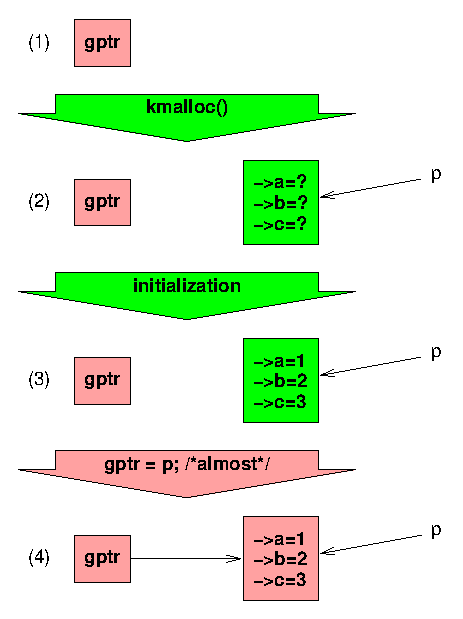
\includegraphics{defer/RCUListInsertClassic}}
\caption{Insertion With Concurrent Readers}
\label{fig:defer:Insertion With Concurrent Readers}
\end{figure}

A classic approach for insertion is shown in
Figure~\ref{fig:defer:Insertion With Concurrent Readers}.
The first row shows the default state, with \co{gptr} equal to \co{NULL}.
In the second row, we have allocated a structure which is uninitialized,
as indicated by the question marks.
In the third row, we have initialized the structure.
Next, we assign \co{gptr} to reference this new element.\footnote{
	On many computer systems, simple assignment is insufficient
	due to interference from both the compiler and the CPU.
	These issues will be covered in
	Section~\ref{sec:defer:RCU Fundamentals}.}
On modern general-purpose systems, this assignment is atomic in the
sense that concurrent readers will see either a \co{NULL} pointer
or a pointer to the new structure \co{p}, but not some mash-up
containing bits from both values.
Each reader is therefore guaranteed to either get the
default value of \co{NULL} or to get the newly installed
non-default values, but either way each reader will see
a consistent result.
Even better, readers need not use any expensive synchronization
primitives, so this approach is quite suitable for real-time use.\footnote{
	Again, on many computer systems, additional work is required
	to prevent interference from the compiler, and, on DEC Alpha
	systems, the CPU as well.
	This will be covered in
	Section~\ref{sec:defer:RCU Fundamentals}.}

\begin{figure}[tb]
\centering
\resizebox{3in}{!}{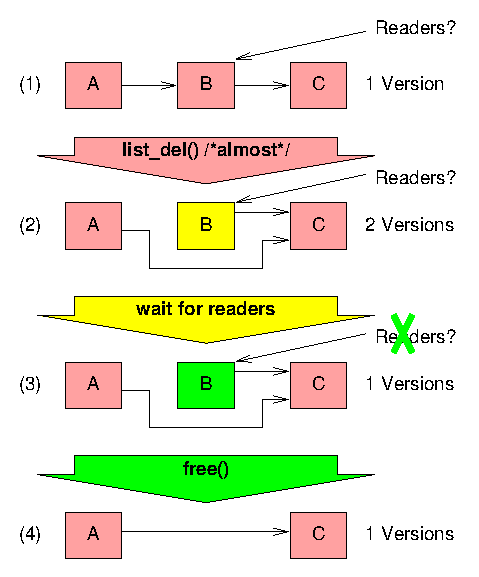
\includegraphics{defer/RCUListDeleteClassic}}
\caption{Deletion From Linked List With Concurrent Readers}
\label{fig:defer:Deletion From Linked List With Concurrent Readers}
\end{figure}

But sooner or later, it will be necessary to remove data that is
being referenced by concurrent readers.
Let us move to a more complex example where we are removing an element
from a linked list, as shown in
Figure~\ref{fig:defer:Deletion From Linked List With Concurrent Readers}.
This list initially contains elements~\co{A}, \co{B}, and \co{C},
and we need to remove element~\co{B}.
First, we use \co{list_del()} to carry out the removal,\footnote{
	And yet again, this approximates reality, which will be expanded
	on in Section~\ref{sec:defer:RCU Fundamentals}.}
at which point all new readers will see element~\co{B} as having been
deleted from the list.
However, there might be old readers still referencing this element.
Once all these old readers have finished, we can safely free
element~\co{B}, resulting in the situation shown at the bottom of
the figure.

But how can we tell when the readers are finished?

It is tempting to consider a reference-counting scheme, but
Figure~\ref{fig:count:Atomic Increment Scalability on Nehalem}
in
Chapter~\ref{chp:Counting}
shows that this can also result in long delays, just as can
the locking and sequence-locking approaches that we already rejected.

Let's consider the logical extreme where the readers do absolutely
nothing to announce their presence.
This approach clearly allows optimal performance for readers
(after all, free is a very good price),
but leaves open the question of how the updater can possibly
determine when all the old readers are done.
We clearly need some additional constraints if we are to provide
a reasonable answer to this question.

One constraint that fits well with some operating-system kernels is to
consider the case where threads are not subject to preemption.
In such non-preemptible environments, each thread runs until it
explicitly and voluntarily blocks.
This means that an infinite loop without blocking will render a CPU
useless for any other purpose from the start of the infinite loop
onwards.\footnote{
	In contrast, an infinite loop in a preemptible environment
	might be preempted.
	This infinite loop might still waste considerable CPU time,
	but the CPU in question would nevertheless be able to do
	other work.}
Non-preemptibility also requires that threads be prohibited from blocking
while holding spinlocks.
Without this prohibition, all CPUs might be consumed by threads
spinning attempting to acquire a spinlock held by a blocked thread.
The spinning threads will not relinquish their CPUs until they acquire
the lock, but the thread holding the lock cannot possibly release it
until one of the spinning threads relinquishes a CPU.
This is a classic deadlock situation.

Let us impose this same constraint on reader threads traversing the
linked list: such threads are not allowed to block until after
completing their traversal.
Returning to the second row of
Figure~\ref{fig:defer:Deletion From Linked List With Concurrent Readers},
where the updater has just completed executing \co{list_del()},
imagine that CPU~0 executes a context switch.
Because readers are not permitted to block while traversing the linked
list, we are guaranteed that all prior readers that might have been running on
CPU~0 will have completed.
Extending this line of reasoning to the other CPUs, once each CPU has
been observed executing a context switch, we are guaranteed that all
prior readers have completed, and that there are no longer any reader
threads referencing element~\co{B}.
The updater can then safely free element~\co{B}, resulting in the
state shown at the bottom of
Figure~\ref{fig:defer:Deletion From Linked List With Concurrent Readers}.

\begin{figure}[tb]
\centering
\resizebox{3in}{!}{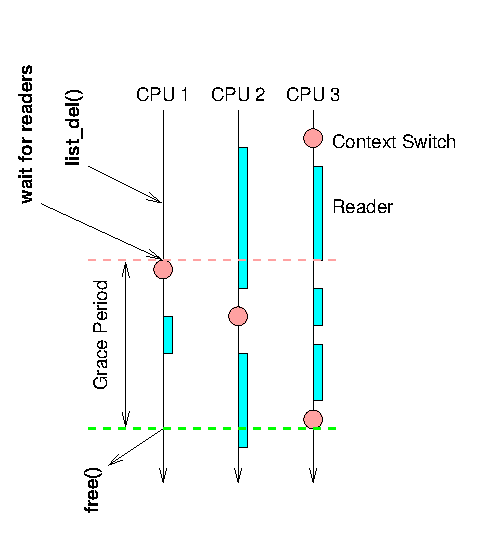
\includegraphics{defer/QSBRGracePeriod}}
\caption{RCU QSBR: Waiting for Pre-Existing Readers}
\label{fig:defer:RCU QSBR: Waiting for Pre-Existing Readers}
\end{figure}

This approach is termed \emph{quiescent state based reclamation}
(QSBR)~\cite{ThomasEHart2006a}.
A QSBR schematic is shown in
Figure~\ref{fig:defer:RCU QSBR: Waiting for Pre-Existing Readers},
with time advancing from the top of the figure to the bottom.

Although production-quality implementations of this approach can be
quite complex, a toy implementation is exceedingly simple:

\vspace{5pt}
\begin{minipage}[t]{\columnwidth}
\scriptsize
\begin{verbatim}
  1 for_each_online_cpu(cpu)
  2   run_on(cpu);
\end{verbatim}
\end{minipage}
\vspace{5pt}

The \co{for_each_online_cpu()} primitive iterates over all CPUs, and
the \co{run_on()} function causes the current thread to execute on the
specified CPU, which forces the destination CPU to execute a context
switch.
Therefore, once the \co{for_each_online_cpu()} has completed, each CPU
has executed a context switch, which in turn guarantees that
all pre-existing reader threads have completed.

Please note that this approach is \emph{not} production quality.
Correct handling of a number of corner cases and the need for a number
of powerful optimizations mean that production-quality implementations
have significant additional complexity.
In addition, RCU implementations for preemptible environments
require that readers actually do something.
However, this simple non-preemptible approach is conceptually complete,
and forms a good initial basis for understanding the RCU fundamentals
covered in the following section.

% defer/rcufundamental.tex

\subsection{RCU Fundamentals}
\label{sec:defer:RCU Fundamentals}
\OriginallyPublished{Section}{sec:defer:RCU Fundamentals}{RCU Fundamentals}{Linux Weekly News}{PaulEMcKenney2007WhatIsRCUFundamentally}

Authors: Paul E. McKenney and Jonathan Walpole

Read-copy update (RCU) is a synchronization mechanism that was added to
the Linux kernel in October of 2002.
RCU achieves scalability
improvements by allowing reads to occur concurrently with updates.
In contrast with conventional locking primitives that ensure mutual exclusion
among concurrent threads regardless of whether they be readers or
updaters, or with reader-writer locks that allow concurrent reads but not in
the presence of updates, RCU supports concurrency between a single
updater and multiple readers.
RCU ensures that reads are coherent by
maintaining multiple versions of objects and ensuring that they are not
freed up until all pre-existing read-side critical sections complete.
RCU defines and uses efficient and scalable mechanisms for publishing
and reading new versions of an object, and also for deferring the collection
of old versions.
These mechanisms distribute the work among read and
update paths in such a way as to make read paths extremely fast. In some
cases (non-preemptible kernels), RCU's read-side primitives have zero
overhead.

\QuickQuiz{}
	But doesn't Section~\ref{sec:defer:Sequence Locks}'s seqlock
	also permit readers and updaters to get work done concurrently?
\QuickQuizAnswer{
	Yes and no.
	Although seqlock readers can run concurrently with
	seqlock writers, whenever this happens, the {\tt read\_seqretry()}
	primitive will force the reader to retry.
	This means that any work done by a seqlock reader running concurrently
	with a seqlock updater will be discarded and redone.
	So seqlock readers can \emph{run} concurrently with updaters,
	but they cannot actually get any work done in this case.

	In contrast, RCU readers can perform useful work even in presence
	of concurrent RCU updaters.
} \QuickQuizEnd

This leads to the question ``what exactly is RCU?'', and perhaps also
to the question ``how can RCU \emph{possibly} work?'' (or, not
infrequently, the assertion that RCU cannot possibly work).
This document addresses these questions from a fundamental viewpoint;
later installments look at them from usage and from API viewpoints.
This last installment also includes a list of references.

RCU is made up of three fundamental mechanisms, the first being
used for insertion, the second being used for deletion, and the third
being used to allow readers to tolerate concurrent insertions and deletions.
Section~\ref{sec:defer:Publish-Subscribe Mechanism}
describes the publish-subscribe mechanism used for insertion,
Section~\ref{sec:defer:Wait For Pre-Existing RCU Readers to Complete}
describes how waiting for pre-existing RCU readers enabled deletion,
and
Section~\ref{sec:defer:Maintain Multiple Versions of Recently Updated Objects}
discusses how maintaining multiple versions of recently updated objects
permits concurrent insertions and deletions.
Finally,
Section~\ref{sec:defer:Summary of RCU Fundamentals}
summarizes RCU fundamentals.

\subsubsection{Publish-Subscribe Mechanism}
\label{sec:defer:Publish-Subscribe Mechanism}

\begin{figure}[tbp]
{ \scriptsize
\begin{verbatim}
  1 struct foo {
  2   int a;
  3   int b;
  4   int c;
  5 };
  6 struct foo *gp = NULL;
  7
  8 /* . . . */
  9
 10 p = kmalloc(sizeof(*p), GFP_KERNEL);
 11 p->a = 1;
 12 p->b = 2;
 13 p->c = 3;
 14 gp = p;
\end{verbatim}
}
\caption{Data Structure Publication (Unsafe)}
\label{fig:defer:Data Structure Publication (Unsafe)}
\end{figure}

One key attribute of RCU is the ability to safely scan data, even
though that data is being modified concurrently.
To provide this ability for concurrent insertion,
RCU uses what can be thought of as a publish-subscribe mechanism.
For example, consider an initially \co{NULL} global pointer
\co{gp} that is to be modified to point to a newly allocated
and initialized data structure.
The code fragment shown in
Figure~\ref{fig:defer:Data Structure Publication (Unsafe)}
(with the addition of appropriate locking)
might be used for this purpose.

Unfortunately, there is nothing forcing the compiler and CPU to execute
the last four assignment statements in order.
If the assignment to \co{gp} happens before the initialization
of \co{p} fields, then concurrent readers could see the
uninitialized values.
Memory barriers are required to keep things ordered, but memory barriers
are notoriously difficult to use.
We therefore encapsulate them into a primitive
\co{rcu_assign_pointer()} that has publication semantics.
The last four lines would then be as follows:

\vspace{5pt}
\begin{minipage}[t]{\columnwidth}
\scriptsize
\begin{verbatim}
  1 p->a = 1;
  2 p->b = 2;
  3 p->c = 3;
  4 rcu_assign_pointer(gp, p);
\end{verbatim}
\end{minipage}
\vspace{5pt}

The \co{rcu_assign_pointer()}
would \emph{publish} the new structure, forcing both the compiler
and the CPU to execute the assignment to \co{gp} \emph{after}
the assignments to the fields referenced by \co{p}.

However, it is not sufficient to only enforce ordering at the
updater, as the reader must enforce proper ordering as well.
Consider for example the following code fragment:

\vspace{5pt}
\begin{minipage}[t]{\columnwidth}
\scriptsize
\begin{verbatim}
  1 p = gp;
  2 if (p != NULL) {
  3   do_something_with(p->a, p->b, p->c);
  4 }
\end{verbatim}
\end{minipage}
\vspace{5pt}

Although this code fragment might well seem immune to misordering,
unfortunately, the
DEC Alpha CPU~\cite{PaulMcKenney2005i,PaulMcKenney2005j}
and value-speculation compiler optimizations can, believe it or not,
cause the values of \co{p->a}, \co{p->b}, and
\co{p->c} to be fetched before the value of \co{p}.
This is perhaps easiest to see in the case of value-speculation
compiler optimizations, where the compiler guesses the value
of \co{p} fetches \co{p->a}, \co{p->b}, and
\co{p->c} then fetches the actual value of \co{p}
in order to check whether its guess was correct.
This sort of optimization is quite aggressive, perhaps insanely so,
but does actually occur in the context of profile-driven optimization.

Clearly, we need to prevent this sort of skullduggery on the
part of both the compiler and the CPU.
The \co{rcu_dereference()} primitive uses
whatever memory-barrier instructions and compiler
directives are required for this purpose:

\vspace{5pt}
\begin{minipage}[t]{\columnwidth}
\scriptsize
\begin{verbatim}
  1 rcu_read_lock();
  2 p = rcu_dereference(gp);
  3 if (p != NULL) {
  4   do_something_with(p->a, p->b, p->c);
  5 }
  6 rcu_read_unlock();
\end{verbatim}
\end{minipage}
\vspace{5pt}

The \co{rcu_dereference()} primitive can thus be thought of
as \emph{subscribing} to a given value of the specified pointer,
guaranteeing that subsequent dereference operations will see any
initialization that occurred before the corresponding
\co{rcu_assign_pointer()} operation that published that pointer.
The \co{rcu_read_lock()} and \co{rcu_read_unlock()}
calls are absolutely required: they define the extent of the
RCU read-side critical section.
Their purpose is explained in
Section~\ref{sec:defer:Wait For Pre-Existing RCU Readers to Complete},
however, they never spin or block, nor do they prevent the
\co{list_add_rcu()} from executing concurrently.
In fact, in non-\co{CONFIG_PREEMPT} kernels, they generate
absolutely no code.

\begin{figure}[tb]
\begin{center}
\resizebox{3in}{!}{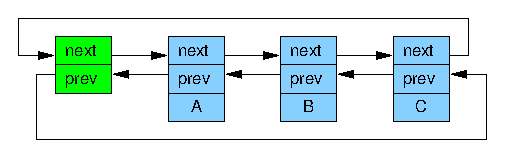
\includegraphics{defer/Linux_list}}
\end{center}
\caption{Linux Circular Linked List}
\label{fig:defer:Linux Circular Linked List}
\end{figure}

\begin{figure}[tb]
\begin{center}
\resizebox{3in}{!}{\includegraphics{defer/Linux_list_abbr}}
\end{center}
\caption{Linux Linked List Abbreviated}
\label{fig:defer:Linux Linked List Abbreviated}
\end{figure}

Although \co{rcu_assign_pointer()} and
\co{rcu_dereference()} can in theory be used to construct any
conceivable RCU-protected data structure, in practice it is often better
to use higher-level constructs.
Therefore, the \co{rcu_assign_pointer()} and
\co{rcu_dereference()}
primitives have been embedded in special RCU variants of Linux's
list-manipulation API.
Linux has two variants of doubly linked list, the circular
{\tt struct list\_head} and the linear
{\tt struct hlist\_head}/{\tt struct hlist\_node} pair.
The former is laid out as shown in
Figure~\ref{fig:defer:Linux Circular Linked List},
where the green boxes represent
the list header and the blue boxes represent the elements in the
list.
This notation is cumbersome, and will therefore be abbreviated as shown in
Figure~\ref{fig:defer:Linux Linked List Abbreviated}.

\begin{figure}[tbp]
{ \scriptsize
\begin{verbatim}
  1 struct foo {
  2   struct list_head *list;
  3   int a;
  4   int b;
  5   int c;
  6 };
  7 LIST_HEAD(head);
  8
  9 /* . . . */
 10
 11 p = kmalloc(sizeof(*p), GFP_KERNEL);
 12 p->a = 1;
 13 p->b = 2;
 14 p->c = 3;
 15 list_add_rcu(&p->list, &head);
\end{verbatim}
}
\caption{RCU Data Structure Publication}
\label{fig:defer:RCU Data Structure Publication}
\end{figure}

Adapting the pointer-publish example for the linked list results in
the code shown in
Figure~\ref{fig:defer:RCU Data Structure Publication}.

Line~15 must be protected by some synchronization mechanism (most
commonly some sort of lock) to prevent multiple \co{list_add()}
instances from executing concurrently.
However, such synchronization does not prevent this \co{list_add()}
instance from executing concurrently with RCU readers.

Subscribing to an RCU-protected list is straightforward:

\vspace{5pt}
\begin{minipage}[t]{\columnwidth}
\scriptsize
\begin{verbatim}
  1 rcu_read_lock();
  2 list_for_each_entry_rcu(p, head, list) {
  3   do_something_with(p->a, p->b, p->c);
  4 }
  5 rcu_read_unlock();
\end{verbatim}
\end{minipage}
\vspace{5pt}

The \co{list_add_rcu()} primitive publishes
an entry into the specified list, guaranteeing that the corresponding
\co{list_for_each_entry_rcu()} invocation will properly
subscribe to this same entry.

\QuickQuiz{}
	What prevents the {\tt list\_for\_each\_entry\_rcu()} from
	getting a segfault if it happens to execute at exactly the same
	time as the {\tt list\_add\_rcu()}?
\QuickQuizAnswer{
	On all systems running Linux, loads from and stores
	to pointers are atomic, that is, if a store to a pointer occurs at
	the same time as a load from that same pointer, the load will return
	either the initial value or the value stored, never some bitwise
	mashup of the two.
	In addition, the {\tt list\_for\_each\_entry\_rcu()} always proceeds
	forward through the list, never looking back.
	Therefore, the {\tt list\_for\_each\_entry\_rcu()} will either see
	the element being added by {\tt list\_add\_rcu()} or it will not,
	but either way, it will see a valid well-formed list.
} \QuickQuizEnd

\begin{figure}[tb]
\begin{center}
\resizebox{3in}{!}{\includegraphics{defer/Linux_hlist}}
\end{center}
\caption{Linux Linear Linked List}
\label{fig:defer:Linux Linear Linked List}
\end{figure}

Linux's other doubly linked list, the hlist,
is a linear list, which means that
it needs only one pointer for the header rather than the two
required for the circular list, as shown in
Figure~\ref{fig:defer:Linux Linear Linked List}.
Thus, use of hlist can halve the memory consumption for the hash-bucket
arrays of large hash tables.
As before, this notation is cumbersome, so hlists will be abbreviated
in the same way lists are, as shown in
Figure~\ref{fig:defer:Linux Linked List Abbreviated}.

\begin{figure}[tbp]
{ \scriptsize
\begin{verbatim}
  1 struct foo {
  2   struct hlist_node *list;
  3   int a;
  4   int b;
  5   int c;
  6 };
  7 HLIST_HEAD(head);
  8
  9 /* . . . */
 10
 11 p = kmalloc(sizeof(*p), GFP_KERNEL);
 12 p->a = 1;
 13 p->b = 2;
 14 p->c = 3;
 15 hlist_add_head_rcu(&p->list, &head);
\end{verbatim}
}
\caption{RCU {\tt hlist} Publication}
\label{fig:defer:RCU hlist Publication}
\end{figure}

Publishing a new element to an RCU-protected hlist is quite similar
to doing so for the circular list,
as shown in Figure~\ref{fig:defer:RCU hlist Publication}.

As before, line~15 must be protected by some sort of synchronization
mechanism, for example, a lock.

Subscribing to an RCU-protected hlist is also similar to the
circular list:

\vspace{5pt}
\begin{minipage}[t]{\columnwidth}
\scriptsize
\begin{verbatim}
  1 rcu_read_lock();
  2 hlist_for_each_entry_rcu(p, q, head, list) {
  3   do_something_with(p->a, p->b, p->c);
  4 }
  5 rcu_read_unlock();
\end{verbatim}
\end{minipage}
\vspace{5pt}

\QuickQuiz{}
	Why do we need to pass two pointers into
	{\tt hlist\_for\_each\_entry\_rcu()}
	when only one is needed for {\tt list\_for\_each\_entry\_rcu()}?
\QuickQuizAnswer{
	Because in an hlist it is necessary to check for
	NULL rather than for encountering the head.
	(Try coding up a single-pointer {\tt hlist\_for\_each\_entry\_rcu()}
	If you come up with a nice solution, it would be a very good thing!)
} \QuickQuizEnd

\begin{table*}[tb]
\begin{center}
\scriptsize
\begin{tabular}{l||l|l|l}
Category  & Publish	& Retract	& Subscribe \\
\hline
\hline
Pointers  & \co{rcu_assign_pointer()}
			& \co{rcu_assign_pointer(..., NULL)}~~
					& \co{rcu_dereference()} \\
\hline
Lists     & \parbox{1.5in}{
		\co{list_add_rcu()} \\
		\co{list_add_tail_rcu()} \\
		\co{list_replace_rcu()} }
			& \co{list_del_rcu()}
					& \co{list_for_each_entry_rcu()}~~~ \\
\hline
Hlists    & \parbox{1.5in}{
		\co{hlist_add_after_rcu()} \\
		\co{hlist_add_before_rcu()}  \\
		\co{hlist_add_head_rcu()} \\
		\co{hlist_replace_rcu()} }
			& \co{hlist_del_rcu()}
					& \co{hlist_for_each_entry_rcu()}~~~~~
\end{tabular}
\end{center}
\caption{RCU Publish and Subscribe Primitives}
\label{tab:defer:RCU Publish and Subscribe Primitives}
\end{table*}

The set of RCU publish and subscribe primitives are shown in
Table~\ref{tab:defer:RCU Publish and Subscribe Primitives},
along with additional primitives to ``unpublish'', or retract.

Note that the \co{list_replace_rcu()}, \co{list_del_rcu()},
\co{hlist_replace_rcu()}, and \co{hlist_del_rcu()}
APIs add a complication.
When is it safe to free up the data element that was replaced or
removed?
In particular, how can we possibly know when all the readers
have released their references to that data element?

These questions are addressed in the following section.

\subsubsection{Wait For Pre-Existing RCU Readers to Complete}
\label{sec:defer:Wait For Pre-Existing RCU Readers to Complete}

In its most basic form, RCU is a way of waiting for things to finish.
Of course, there are a great many other ways of waiting for things to
finish, including reference counts, reader-writer locks, events, and so on.
The great advantage of RCU is that it can wait for each of
(say) 20,000 different things without having to explicitly
track each and every one of them, and without having to worry about
the performance degradation, scalability limitations, complex deadlock
scenarios, and memory-leak hazards that are inherent in schemes
using explicit tracking.

In RCU's case, the things waited on are called
``RCU read-side critical sections''.
An RCU read-side critical section starts with an
\co{rcu_read_lock()} primitive, and ends with a corresponding
\co{rcu_read_unlock()} primitive.
RCU read-side critical sections can be nested, and may contain pretty
much any code, as long as that code does not explicitly block or sleep
(although a special form of RCU called SRCU~\cite{PaulEMcKenney2006c}
does permit general sleeping in SRCU read-side critical sections).
If you abide by these conventions, you can use RCU to wait for \emph{any}
desired piece of code to complete.

RCU accomplishes this feat by indirectly determining when these
other things have finished~\cite{PaulEMcKenney2007whatisRCU,
PaulEMcKenney2007PreemptibleRCU}, as is described in detail in
Appendix~\ref{app:rcuimpl:Read-Copy Update Implementations}.

\begin{figure}[tb]
\begin{center}
\resizebox{3in}{!}{\includegraphics{defer/GracePeriodGood}}
\end{center}
\caption{Readers and RCU Grace Period}
\label{fig:defer:Readers and RCU Grace Period}
\end{figure}

In particular, as shown in
Figure~\ref{fig:defer:Readers and RCU Grace Period},
RCU is a way of
waiting for pre-existing RCU read-side critical sections to completely
finish, including memory operations executed by those critical sections.
However, note that RCU read-side critical sections
that begin after the beginning
of a given grace period can and will extend beyond the end of that grace
period.

The following pseudocode shows the basic form of algorithms that use
RCU to wait for readers:

\begin{enumerate}
\item	Make a change, for example, replace an element in a linked list.
\item	Wait for all pre-existing RCU read-side critical sections to
	completely finish (for example, by using the
	\co{synchronize_rcu()} primitive).
	The key observation here is that subsequent RCU read-side critical
	sections have no way to gain a reference to the newly removed
	element.
\item	Clean up, for example, free the element that was replaced above.
\end{enumerate}

\begin{figure}[tbp]
{ \scriptsize
\begin{verbatim}
  1 struct foo {
  2   struct list_head *list;
  3   int a;
  4   int b;
  5   int c;
  6 };
  7 LIST_HEAD(head);
  8
  9 /* . . . */
 10
 11 p = search(head, key);
 12 if (p == NULL) {
 13   /* Take appropriate action, unlock, & return. */
 14 }
 15 q = kmalloc(sizeof(*p), GFP_KERNEL);
 16 *q = *p;
 17 q->b = 2;
 18 q->c = 3;
 19 list_replace_rcu(&p->list, &q->list);
 20 synchronize_rcu();
 21 kfree(p);
\end{verbatim}
}
\caption{Canonical RCU Replacement Example}
\label{fig:defer:Canonical RCU Replacement Example}
\end{figure}

The code fragment shown in
Figure~\ref{fig:defer:Canonical RCU Replacement Example},
adapted from those in Section~\ref{sec:defer:Publish-Subscribe Mechanism},
demonstrates this process, with field \co{a} being the search key.

Lines~19, 20, and 21 implement the three steps called out above.
Lines~16-19 gives RCU (``read-copy update'') its name: while permitting
concurrent \emph{reads}, line~16 \emph{copies} and lines~17-19
do an \emph{update}.

As discussed in Section~\ref{sec:defer:Introduction to RCU},
the \co{synchronize_rcu()} primitive can be quite simple
(see Section~\ref{sec:defer:``Toy'' RCU Implementations}
for additional ``toy'' RCU implementations).
However, production-quality implementations must deal with
difficult corner cases and also incorporate
powerful optimizations, both of which result in significant complexity.
Although it is good to know that there is a simple conceptual
implementation of \co{synchronize_rcu()}, other questions remain.
For example, what exactly do RCU
readers see when traversing a concurrently updated list?
This question is addressed in the following section.

\subsubsection{Maintain Multiple Versions of Recently Updated Objects}
\label{sec:defer:Maintain Multiple Versions of Recently Updated Objects}

This section demonstrates how RCU maintains multiple versions of
lists to accommodate synchronization-free readers.
Two examples are presented showing how an element
that might be referenced by a given reader must remain intact
while that reader remains in its RCU read-side critical section.
The first example demonstrates deletion of a list element,
and the second example demonstrates replacement of an element.

\paragraph{Example 1: Maintaining Multiple Versions During Deletion}
\label{sec:defer:Example 1: Maintaining Multiple Versions During Deletion}

We can now revisit the deletion example from
Section~\ref{sec:defer:Introduction to RCU},
but now with the benefit of a firm understanding of the fundamental
concepts underlying RCU.
To begin this new version of the deletion example,
we will modify lines~11-21 in
Figure~\ref{fig:defer:Canonical RCU Replacement Example}
to read as follows:

\vspace{5pt}
\begin{minipage}[t]{\columnwidth}
\scriptsize
\begin{verbatim}
  1 p = search(head, key);
  2 if (p != NULL) {
  3   list_del_rcu(&p->list);
  4   synchronize_rcu();
  5   kfree(p);
  6 }
\end{verbatim}
\end{minipage}
\vspace{5pt}

\begin{figure}[tb]
\begin{center}
\resizebox{3in}{!}{\includegraphics{defer/RCUDeletion}}
\end{center}
\caption{RCU Deletion From Linked List}
\label{fig:defer:RCU Deletion From Linked List}
\end{figure}

This code will update the list as shown in
Figure~\ref{fig:defer:RCU Deletion From Linked List}.
The triples in each element represent the values of fields \co{a},
\co{b}, and \co{c}, respectively.
The red-shaded elements
indicate that RCU readers might be holding references to them.
Please note that
we have omitted the backwards pointers and the link from the tail
of the list to the head for clarity.

After the \co{list_del_rcu()} on
line~3 has completed, the \co{5,6,7}~element
has been removed from the list, as shown in the second row of
Figure~\ref{fig:defer:RCU Deletion From Linked List}.
Since readers do not synchronize directly with updaters,
readers might be concurrently scanning this list.
These concurrent readers might or might not see the newly removed element,
depending on timing.
However, readers that were delayed (e.g., due to interrupts, ECC memory
errors, or, in \co{CONFIG_PREEMPT_RT} kernels, preemption)
just after fetching a pointer to the newly removed element might
see the old version of the list for quite some time after the
removal.
Therefore, we now have two versions of the list, one with element
\co{5,6,7} and one without.
The \co{5,6,7}~element is
shaded yellow, indicating
that old readers might still be referencing it, but that new
readers cannot obtain a reference to it.

Please note that readers are not permitted to maintain references to
element~\co{5,6,7} after exiting from their RCU read-side
critical sections.
Therefore,
once the \co{synchronize_rcu()} on
line~4 completes, so that all pre-existing readers are
guaranteed to have completed,
there can be no more readers referencing this
element, as indicated by its green shading on the third row of
Figure~\ref{fig:defer:RCU Deletion From Linked List}.
We are thus back to a single version of the list.

At this point, the \co{5,6,7}~element may safely be
freed, as shown on the final row of
Figure~\ref{fig:defer:RCU Deletion From Linked List}.
At this point, we have completed the deletion of
element~\co{5,6,7}.
The following section covers replacement.

\paragraph{Example 2: Maintaining Multiple Versions During Replacement}
\label{sec:defer:Example 2: Maintaining Multiple Versions During Replacement}

To start the replacement example,
here are the last few lines of the
example shown in
Figure~\ref{fig:defer:Canonical RCU Replacement Example}:

\vspace{5pt}
\begin{minipage}[t]{\columnwidth}
\scriptsize
\begin{verbatim}
  1 q = kmalloc(sizeof(*p), GFP_KERNEL);
  2 *q = *p;
  3 q->b = 2;
  4 q->c = 3;
  5 list_replace_rcu(&p->list, &q->list);
  6 synchronize_rcu();
  7 kfree(p);
\end{verbatim}
\end{minipage}
\vspace{5pt}

\begin{figure}[tbp]
\begin{center}
\resizebox{2.7in}{!}{\includegraphics{defer/RCUReplacement}}
\end{center}
\caption{RCU Replacement in Linked List}
\label{fig:defer:RCU Replacement in Linked List}
\end{figure}

The initial state of the list, including the pointer \co{p},
is the same as for the deletion example, as shown on the
first row of
Figure~\ref{fig:defer:RCU Replacement in Linked List}.

As before,
the triples in each element represent the values of fields \co{a},
\co{b}, and \co{c}, respectively.
The red-shaded elements might be referenced by readers,
and because readers do not synchronize directly with updaters,
readers might run concurrently with this entire replacement process.
Please note that
we again omit the backwards pointers and the link from the tail
of the list to the head for clarity.

The following text describes how to replace the \co{5,6,7} element
with \co{5,2,3} in such a way that any given reader sees one of these
two values.

Line~1 \co{kmalloc()}s a replacement element, as follows,
resulting in the state as shown in the second row of
Figure~\ref{fig:defer:RCU Replacement in Linked List}.
At this point, no reader can hold a reference to the newly allocated
element (as indicated by its green shading), and it is uninitialized
(as indicated by the question marks).

Line~2 copies the old element to the new one, resulting in the
state as shown in the third row of
Figure~\ref{fig:defer:RCU Replacement in Linked List}.
The newly allocated element still cannot be referenced by readers, but
it is now initialized.

Line~3 updates \co{q->b} to the value ``2'', and
line~4 updates \co{q->c} to the value ``3'', as shown on the fourth row of
Figure~\ref{fig:defer:RCU Replacement in Linked List}.

Now, line~5 does the replacement, so that the new element is
finally visible to readers, and hence is shaded red, as shown on
the fifth row of
Figure~\ref{fig:defer:RCU Replacement in Linked List}.
At this point, as shown below, we have two versions of the list.
Pre-existing readers might see the \co{5,6,7} element (which is
therefore now shaded yellow), but
new readers will instead see the \co{5,2,3} element.
But any given reader is guaranteed to see some well-defined list.

After the \co{synchronize_rcu()} on line~6 returns,
a grace period will have elapsed, and so all reads that started before the
\co{list_replace_rcu()} will have completed.
In particular, any readers that might have been holding references
to the \co{5,6,7} element are guaranteed to have exited
their RCU read-side critical sections, and are thus prohibited from
continuing to hold a reference.
Therefore, there can no longer be any readers holding references
to the old element, as indicated its green shading in the sixth row of
Figure~\ref{fig:defer:RCU Replacement in Linked List}.
As far as the readers are concerned, we are back to having a single version
of the list, but with the new element in place of the old.

After the \co{kfree()} on line 7 completes, the list will
appear as shown on the final row of
Figure~\ref{fig:defer:RCU Replacement in Linked List}.

Despite the fact that RCU was named after the replacement case,
the vast majority of RCU usage within the Linux kernel relies on
the simple deletion case shown in
Section~\ref{sec:defer:Maintain Multiple Versions of Recently Updated Objects}.

\paragraph{Discussion}
\label{sec:defer:Discussion}

These examples assumed that a mutex was held across the entire
update operation, which would mean that there could be at most two
versions of the list active at a given time.

\QuickQuiz{}
	How would you modify the deletion example to permit more than two
	versions of the list to be active?
\QuickQuizAnswer{
	One way of accomplishing this is as shown in
	Figure~\ref{fig:defer:Concurrent RCU Deletion}.

\begin{figure}[htbp]
{ \centering
\begin{verbatim}
  1 spin_lock(&mylock);
  2 p = search(head, key);
  3 if (p == NULL)
  4   spin_unlock(&mylock);
  5 else {
  6   list_del_rcu(&p->list);
  7   spin_unlock(&mylock);
  8   synchronize_rcu();
  9   kfree(p);
 10 }
\end{verbatim}
}
\caption{Concurrent RCU Deletion}
\label{fig:defer:Concurrent RCU Deletion}
\end{figure}

	Note that this means that multiple concurrent deletions might be
	waiting in {\tt synchronize\_rcu()}.
} \QuickQuizEnd

\QuickQuiz{}
	How many RCU versions of a given list can be
	active at any given time?
\QuickQuizAnswer{
	That depends on the synchronization design.
	If a semaphore protecting the update is held across the grace period,
	then there can be at most two versions, the old and the new.

	However, if only the search, the update, and the
	{\tt list\_replace\_rcu()} were protected by a lock, then
	there could be an arbitrary number of versions active, limited only
	by memory and by how many updates could be completed within a
	grace period.
	But please note that data structures that are updated so frequently
	probably are not good candidates for RCU.
	That said, RCU can handle high update rates when necessary.
} \QuickQuizEnd

This sequence of events shows how RCU updates use multiple versions
to safely carry out changes in presence of concurrent readers.
Of course, some algorithms cannot gracefully handle multiple versions.
There are techniques
for adapting such algorithms to RCU~\cite{PaulEdwardMcKenneyPhD},
but these are beyond the scope of this section.

\subsubsection{Summary of RCU Fundamentals}
\label{sec:defer:Summary of RCU Fundamentals}

This section has described the three fundamental components of RCU-based
algorithms:

\begin{enumerate}
\item	a publish-subscribe mechanism for adding new data,

\item	a way of waiting for pre-existing RCU readers to finish, and

\item	a discipline of maintaining multiple versions to permit
	change without harming or unduly delaying concurrent RCU readers.
\end{enumerate}

\QuickQuiz{}
	How can RCU updaters possibly delay RCU readers, given that the
	{\tt rcu\_read\_lock()} and {\tt rcu\_read\_unlock()}
	primitives neither spin nor block?
\QuickQuizAnswer{
	The modifications undertaken by a given RCU updater will cause the
	corresponding CPU to invalidate cache lines containing the data,
	forcing the CPUs running concurrent RCU readers to incur expensive
	cache misses.
	(Can you design an algorithm that changes a data structure
	\emph{without}
	inflicting expensive cache misses on concurrent readers?
	On subsequent readers?)
} \QuickQuizEnd

These three RCU components
allow data to be updated in face of concurrent readers, and
can be combined in different ways to
implement a surprising variety of different types of RCU-based algorithms,
some of which are described in the following section.

% defer/rcuusage.tex

\subsection{RCU Usage}
\label{sec:defer:RCU Usage}

\begin{table}[tb]
\begin{center}
\scriptsize
\begin{tabular}{l|l}
Mechanism RCU Replaces & Section \\
\hline
\hline
Reader-writer locking &
	Section~\ref{sec:defer:RCU is a Reader-Writer Lock Replacement} \\
Restricted reference-counting mechanism &
	Section~\ref{sec:defer:RCU is a Restricted Reference-Counting Mechanism} \\
Bulk reference-counting mechanism &
	Section~\ref{sec:defer:RCU is a Bulk Reference-Counting Mechanism} \\
Poor man's garbage collector &
	Section~\ref{sec:defer:RCU is a Poor Man's Garbage Collector} \\
Existence Guarantees &
	Section~\ref{sec:defer:RCU is a Way of Providing Existence Guarantees} \\
Type-Safe Memory &
	Section~\ref{sec:deferRCU is a Way of Providing Type-Safe Memory} \\
Wait for things to finish &
	Section~\ref{sec:deferRCU is a Way of Waiting for Things to Finish} \\
\end{tabular}
\end{center}
\caption{RCU Usage}
\label{tab:defer:RCU Usage}
\end{table}

This section answers the question "what is RCU?" from the viewpoint
of the uses to which RCU can be put.
Because RCU is most frequently used to replace some existing mechanism,
we look at it primarily in terms of its relationship to such mechanisms,
as listed in Table~\ref{tab:defer:RCU Usage}.
Following the sections listed in this table,
Section~\ref{sec:defer:RCU Usage Summary} provides a summary.

\subsubsection{RCU is a Reader-Writer Lock Replacement}
\label{sec:defer:RCU is a Reader-Writer Lock Replacement}

Perhaps the most common use of RCU within the Linux kernel is as
a replacement for reader-writer locking in read-intensive situations.
Nevertheless, this use of RCU was not immediately apparent to me
at the outset, in fact, I chose to implement something similar to
\url{brlock} before implementing a general-purpose RCU implementation
back in the early 1990s.
Each and every one of the uses I envisioned for the proto-brlock
primitive was instead implemented using RCU.
In fact, it was more than
three years before the proto-\url{brlock} primitive saw its first use.
Boy, did I feel foolish!

The key similarity between RCU and reader-writer locking is that
both have read-side critical sections that can execute in parallel.
In fact, in some cases, it is possible to mechanically substitute RCU API
members for the corresponding reader-writer lock API members.
But first, why bother?

Advantages of RCU include performance,
deadlock immunity, and realtime latency.
There are, of course, limitations to RCU, including the fact that
readers and updaters run concurrently, that low-priority RCU readers
can block high-priority threads waiting for a grace period to elapse,
and that grace-period latencies can extend for many milliseconds.
These advantages and limitations are discussed in the following sections.

\paragraph{Performance}

\begin{figure}[tb]
\begin{center}
\resizebox{3in}{!}{\includegraphics{defer/rwlockRCUperf}}
\end{center}
\caption{Performance Advantage of RCU Over Reader-Writer Locking}
\label{fig:defer:Performance Advantage of RCU Over Reader-Writer Locking}
\end{figure}

The read-side performance advantages of RCU over reader-writer locking
are shown in
Figure~\ref{fig:defer:Performance Advantage of RCU Over Reader-Writer Locking}.

\QuickQuiz{
WTF???
How the heck do you expect me to believe that RCU has a
100-femtosecond overhead when the clock period at 3GHz is more than
300 \emph{picoseconds}?}
\QuickQuizAnswer{
First, consider that the inner loop used to
take this measurement is as follows:

\vspace{5pt}
\begin{minipage}[t]{\columnwidth}
\small
\begin{verbatim}
  1 for (i = 0; i < CSCOUNT_SCALE; i++) {
  2   rcu_read_lock();
  3   rcu_read_unlock();
  4 }
\end{verbatim}
\end{minipage}
\vspace{5pt}

Next, consider the effective definitions of \url{rcu_read_lock()}
and \url{rcu_read_unlock()}:

\vspace{5pt}
\begin{minipage}[t]{\columnwidth}
\small
\begin{verbatim}
  1 #define rcu_read_lock()   do { } while (0)
  2 #define rcu_read_unlock() do { } while (0)
\end{verbatim}
\end{minipage}
\vspace{5pt}

Consider also that the compiler does simple optimizations,
allowing it to replace the loop with:

\vspace{5pt}
\begin{minipage}[t]{\columnwidth}
\small
\begin{verbatim}
i = CSCOUNT_SCALE;
\end{verbatim}
\end{minipage}
\vspace{5pt}

So the "measurement" of 100 femtoseconds is simply the fixed
overhead of the timing measurements divided by the number of
passes through the inner loop containing the calls
to \url{rcu_read_lock()} and \url{rcu_read_unlock()}.
And therefore, this measurement really is in error, in fact,
in error by an arbitrary number of orders of magnitude.
As you can see by the definition of \url{rcu_read_lock()}
and \url{rcu_read_unlock()} above, the actual overhead
is precisely zero.

It certainly is not every day that a timing measurement of
100 femtoseconds turns out to be an overestimate!
} \QuickQuizEnd

Note that reader-writer locking is orders of magnitude slower than RCU
on a single CPU, and is almost two \emph{additional} orders of magnitude
slower on 16 CPUs.
In contrast, RCU scales quite well.
In both cases, the error bars span a single standard deviation in either
direction.

\begin{figure}[tb]
\begin{center}
\resizebox{3in}{!}{\includegraphics{defer/rwlockRCUperfPREEMPT}}
\end{center}
\caption{Performance Advantage of Preemptable RCU Over Reader-Writer Locking}
\label{fig:defer:Performance Advantage of Preemptable RCU Over Reader-Writer Locking}
\end{figure}

A more moderate view may be obtained from a \url{CONFIG_PREEMPT}
kernel, though RCU still beats reader-writer locking by between one and
three orders of magnitude, as shown in
Figure~\ref{fig:defer:Performance Advantage of Preemptable RCU Over Reader-Writer Locking}.
Note the high variability of reader-writer locking at larger numbers of CPUs.
The error bars span a single standard deviation in either direction.

\begin{figure}[tb]
\begin{center}
\resizebox{3in}{!}{\includegraphics{defer/rwlockRCUperfwtPREEMPT}}
\end{center}
\caption{Comparison of RCU to Reader-Writer Locking as Function of Critical-Section Duration}
\label{fig:defer:Comparison of RCU to Reader-Writer Locking as Function of Critical-Section Duration}
\end{figure}

Of course, the low performance of reader-writer locking in
Figure~\ref{fig:defer:Performance Advantage of Preemptable RCU Over Reader-Writer Locking}
is exaggerated by the unrealistic zero-length critical sections.
The performance advantages of RCU become less significant as the overhead
of the critical section increases, as shown in
Figure~\ref{fig:defer:Comparison of RCU to Reader-Writer Locking as Function of Critical-Section Duration}
for a 16-CPU system,
in which the y-axis represents the sum of the overhead
of the read-side primitives and that of the critical section.

\QuickQuiz{
Why does both the variability and overhead of rwlock decrease as the
critical-section overhead increases?}
\QuickQuizAnswer{
Because the contention on the underlying
\url{rwlock_t} decreases as the critical-section overhead
increases.
However, the rwlock overhead will not quite drop to that on a single
CPU because of cache-thrashing overhead.
} \QuickQuizEnd

However, this observation must be tempered by the fact that
a number of system calls (and thus any RCU read-side critical sections
that they contain) can complete within a few microseconds.

In addition, as is discussed in the next section,
RCU read-side primitives are almost entirely deadlock-immune.


\paragraph{Deadlock Immunity}

Although RCU offers significant performance advantages for
read-mostly workloads, one of the primary reasons for creating
RCU in the first place was in fact its immunity to read-side
deadlocks.
This immunity stems from the fact that
RCU read-side primitives do not block, spin, or even
do backwards branches, so that their execution time is deterministic.
It is therefore impossible for them to participate in a deadlock
cycle.

\QuickQuiz{
Is there an exception to this deadlock immunity, and if so,
what sequence of events could lead to deadlock?}
\QuickQuizAnswer{
One way to cause a deadlock cycle involving
RCU read-side primitives is via the following (illegal) sequence
of statements:

\vspace{5pt}
\begin{minipage}[t]{\columnwidth}
\small
\begin{verbatim}
idx = srcu_read_lock(&srcucb);
synchronize_srcu(&srcucb);
srcu_read_unlock(&srcucb, idx);
\end{verbatim}
\end{minipage}
\vspace{5pt}

The \url{synchronize_rcu()} cannot return until all
pre-existing SRCU read-side critical sections complete, but
is enclosed in an SRCU read-side critical section that cannot
complete until the \url{synchronize_srcu()} returns.
The result is a classic self-deadlock--you get the same
effect when attempting to write-acquire a reader-writer lock
while read-holding it.

Note that this self-deadlock scenario does not apply to
RCU Classic, because the context switch performed by the
\url{synchronize_rcu()} would act as a quiescent state
for this CPU, allowing a grace period to complete.
However, this is if anything even worse, because data used
by the RCU read-side critical section might be freed as a
result of the grace period completing.

In short, do not invoke synchronous RCU update-side primitives
from within an RCU read-side critical section.
} \QuickQuizEnd

An interesting consequence of RCU's read-side deadlock immunity is
that it is possible to unconditionally upgrade an RCU
reader to an RCU updater.
Attempting to do such an upgrade with reader-writer locking results
in deadlock.
A sample code fragment that does an RCU read-to-update upgrade follows:

\vspace{5pt}
\begin{minipage}[t]{\columnwidth}
\scriptsize
\begin{verbatim}
  1 rcu_read_lock();
  2 list_for_each_entry_rcu(p, \&head, list_field) {
  3   do_something_with(p);
  4   if (need_update(p)) {
  5     spin_lock(\my_lock);
  6     do_update(p);
  7     spin_unlock(\&my_lock);
  8   }
  9 }
 10 rcu_read_unlock();
\end{verbatim}
\end{minipage}
\vspace{5pt}

Note that \url{do_update()} is executed under
the protection of the lock \emph{and} under RCU read-side protection.

Another interesting consequence of RCU's deadlock immunity is its
immunity to a large class of priority inversion problems.
For example, low-priority RCU readers cannot prevent a high-priority
RCU updater from acquiring the update-side lock.
Similarly, a low-priority RCU updater cannot prevent high-priority
RCU readers from entering an RCU read-side critical section.

\paragraph{Realtime Latency}

Because RCU read-side primitives neither spin nor block, they offer
excellent realtime latencies.
In addition, as noted earlier, this means that they are
immune to priority inversion
involving the RCU read-side primitives and locks.

However, RCU is susceptible to more subtle priority-inversion scenarios,
for example, a high-priority process blocked waiting for an RCU
grace period to elapse can be blocked by low-priority RCU readers
in -rt kernels.
This can be solved by using RCU priority
boosting~\cite{PaulEMcKenney2007BoostRCU,DinakarGuniguntala2008IBMSysJ}.

\paragraph{RCU Readers and Updaters Run Concurrently}

Because RCU readers never spin nor block, and because updaters are not
subject to any sort of rollback or abort semantics, RCU readers and
updaters must necessarily run concurrently.
This means that RCU readers might access stale data, and might even
see inconsistencies, either of which can render conversion from reader-writer
locking to RCU non-trivial.

\begin{figure}[tb]
\begin{center}
\resizebox{3in}{!}{\includegraphics{defer/rwlockRCUupdate}}
\end{center}
\caption{Response Time of RCU vs. Reader-Writer Locking}
\label{fig:defer:Response Time of RCU vs. Reader-Writer Locking}
\end{figure}

However, in a surprisingly large number of situations, inconsistencies and
stale data are not problems.
The classic example is the networking routing table.
Because routing updates can take considerable time to reach a given
system (seconds or even minutes), the system will have been sending
packets the wrong way for quite some time when the update arrives.
It is usually not a problem to continue sending updates the wrong
way for a few additional milliseconds.
Furthermore, because RCU updaters can make changes without waiting for
RCU readers to finish,
the RCU readers might well see the change more quickly than would
batch-fair
reader-writer-locking readers, as shown in
Figure~\ref{fig:defer:Response Time of RCU vs. Reader-Writer Locking}.

Once the update is received, the rwlock writer cannot proceed until the
last reader completes, and subsequent readers cannot proceed until the
writer completes.
However, these subsequent readers are guaranteed to see the new value,
as indicated by the green background.
In contrast, RCU readers and updaters do not block each other, which permits
the RCU readers to see the updated values sooner.
Of course, because their execution overlaps that of the RCU updater,
\emph{all} of the RCU readers might well see updated values, including
the three readers that started before the update.
Nevertheless only the RCU readers with green backgrounds
are \emph{guaranteed} to see the updated values, again, as indicated
by the green background.

Reader-writer locking and RCU simply provide different guarantees.
With reader-writer locking, any reader that begins after the writer begins
is guaranteed to see new values, and any reader that attempts to
begin while the writer is spinning might or might not see new values,
depending on the reader/writer preference of the rwlock implementation in
question.
In contrast, with RCU, any reader that begins after the updater completes
is guaranteed to see new values, and any reader that completes after the
updater begins might or might not see new values, depending on timing.

The key point here is that, although reader-writer locking does
indeed guarantee consistency within the confines of the computer system,
there are situations where this consistency comes at the price of
increased \emph{inconsistency} with the outside world.
In other words, reader-writer locking obtains internal consistency at the
price of silently stale data with respect to the outside world.

Nevertheless, there are situations where inconsistency and stale
data within the confines of the system cannot be tolerated.
Fortunately,
there are a number of approaches that avoid inconsistency and stale
data~\cite{PaulEdwardMcKenneyPhD,Arcangeli03}, and some
methods based on reference counting are discussed in
Section~@@@.

\paragraph{Low-Priority RCU Readers Can Block High-Priority Reclaimers}

In Realtime RCU~\cite{DinakarGuniguntala2008IBMSysJ},
SRCU~\cite{PaulEMcKenney2006c}, or
QRCU~\cite{PaulEMcKenney2007QRCUspin},
each of which is described in
the final installment of this series,
a preempted reader will prevent
a grace period from completing, even if a high-priority task is
blocked waiting for that grace period to complete.
Realtime RCU can avoid this problem by substituting \url{call_rcu()}
for \url{synchronize_rcu()} or by using RCU priority
boosting~\cite{PaulEMcKenney2007BoostRCU,DinakarGuniguntala2008IBMSysJ}.
which is still in experimental status as of early 2008.
It might become necessary to augment SRCU and QRCU with priority boosting,
but not before a clear real-world need is demonstrated.

\paragraph{RCU Grace Periods Extend for Many Milliseconds}

With the exception of QRCU, RCU grace periods extend for multiple
milliseconds.
Although there are a number of techniques to render such long delays
harmless, including use of the asynchronous interfaces where available
(\url{call_rcu()} and \url{call_rcu_bh()}), this situation
is a major reason for the rule of thumb that RCU be used in read-mostly
situations.

\paragraph{Comparison of Reader-Writer Locking and RCU Code}

In the best case, the conversion from reader-writer locking to RCU
is quite simple, as shown in
Figures~\ref{fig:defer:Converting Reader-Writer Locking to RCU: Data},
\ref{fig:defer:Converting Reader-Writer Locking to RCU: Search},
and
\ref{fig:defer:Converting Reader-Writer Locking to RCU: Deletion},
all taken from
Wikipedia~\cite{WikipediaRCU}.

\begin{figure*}[htbp]
{ \scriptsize \centering
\begin{verbatim}
 1 struct el {                           1 struct el {
 2   struct list_head lp;                2   struct list_head lp;
 3   long key;                           3   long key;
 4   spinlock_t mutex;                   4   spinlock_t mutex;
 5   int data;                           5   int data;
 6   /* Other data fields */             6   /* Other data fields */
 7 };                                    7 };
 8 DEFINE_RWLOCK(listmutex);             8 DEFINE_SPINLOCK(listmutex);
 9 LIST_HEAD(head);                      9 LIST_HEAD(head);
\end{verbatim}
}
\caption{Converting Reader-Writer Locking to RCU: Data}
\label{fig:defer:Converting Reader-Writer Locking to RCU: Data}
\end{figure*}

\begin{figure*}[htbp]
{ \scriptsize \centering
\begin{verbatim}
 1 int search(long key, int *result)     1 int search(long key, int *result)
 2 {                                     2 {
 3   struct el *p;                       3   struct el *p;
 4                                       4
 5   read_lock(&listmutex);              5   rcu_read_lock();
 6   list_for_each_entry(p, &head, lp) { 6   list_for_each_entry_rcu(p, &head, lp) {
 7     if (p->key == key) {              7     if (p->key == key) {
 8       *result = p->data;              8       *result = p->data;
 9       read_unlock(&listmutex);        9       rcu_read_unlock();
10       return 1;                      10       return 1;
11     }                                11     }
12   }                                  12   }
13   read_unlock(&listmutex);           13   rcu_read_unlock();
14   return 0;                          14   return 0;
15 }                                    15 }
\end{verbatim}
}
\caption{Converting Reader-Writer Locking to RCU: Search}
\label{fig:defer:Converting Reader-Writer Locking to RCU: Search}
\end{figure*}

\begin{figure*}[htbp]
{ \scriptsize \centering
\begin{verbatim}
 1 int delete(long key)                  1 int delete(long key)
 2 {                                     2 {
 3   struct el *p;                       3   struct el *p;
 4                                       4
 5   write_lock(&listmutex);             5   spin_lock(&listmutex);
 6   list_for_each_entry(p, &head, lp) { 6   list_for_each_entry(p, &head, lp) {
 7     if (p->key == key) {              7     if (p->key == key) {
 8       list_del(&p->lp);               8       list_del_rcu(&p->lp);
 9       write_unlock(&listmutex);       9       spin_unlock(&listmutex);
                                        10       synchronize_rcu();
10       kfree(p);                      11       kfree(p);
11       return 1;                      12       return 1;
12     }                                13     }
13   }                                  14   }
14   write_unlock(&listmutex);          15   spin_unlock(&listmutex);
15   return 0;                          16   return 0;
16 }                                    17 }
\end{verbatim}
}
\caption{Converting Reader-Writer Locking to RCU: Deletion}
\label{fig:defer:Converting Reader-Writer Locking to RCU: Deletion}
\end{figure*}

More-elaborate cases of replacing reader-writer locking with RCU
are beyond the scope of this document.

\subsubsection{RCU is a Restricted Reference-Counting Mechanism}
\label{sec:defer:RCU is a Restricted Reference-Counting Mechanism}

Because grace periods are not allowed to complete while
there is an RCU read-side critical section in progress,
the RCU read-side primitives may be used as a restricted
reference-counting mechanism.
For example, consider the following code fragment:

\vspace{5pt}
\begin{minipage}[t]{\columnwidth}
\scriptsize
\begin{verbatim}
  1 rcu_read_lock();  /* acquire reference. */
  2 p = rcu_dereference(head);
  3 /* do something with p. */
  4 rcu_read_unlock();  /* release reference. */
\end{verbatim}
\end{minipage}
\vspace{5pt}

The \url{rcu_read_lock()} primitive can be thought of as
acquiring a reference to \url{p}, because a grace period
starting after the \url{rcu_dereference()} assigns to \url{p}
cannot possibly end until after we reach the matching
\url{rcu_read_unlock()}.
This reference-counting scheme is restricted in that
we are not allowed to block in RCU read-side critical sections,
nor are we permitted to hand off an RCU read-side critical section
from one task to another.

Regardless of these restrictions,
the following code can safely delete \url{p}:

\vspace{5pt}
\begin{minipage}[t]{\columnwidth}
\scriptsize
\begin{verbatim}
  1 spin_lock(\&mylock);
  2 p = head;
  3 rcu_assign_pointer(head, NULL);
  4 spin_unlock(\&mylock);
  5 /* Wait for all references to be released. */
  6 synchronize_rcu();
  7 kfree(p);
\end{verbatim}
\end{minipage}
\vspace{5pt}

The assignment to \url{head} prevents any future references
to \url{p} from being acquired, and the \url{synchronize_rcu()}
waits for any previously acquired references to be released.

\QuickQuiz{
But wait!
This is exactly the same code that might be used when thinking
of RCU as a replacement for reader-writer locking!
What gives?}
\QuickQuizAnswer{
This is an effect of the Law of Toy Examples:
beyond a certain point, the code fragments look the same.
The only difference is in how we think about the code.
However, this difference can be extremely important.
For but one example of the importance, consider that if we think
of RCU as a restricted reference counting scheme, we would never
be fooled into thinking that the updates would exclude the RCU
read-side critical sections.
\\ ~ \\
It nevertheless is often useful to think of RCU as a replacement
for reader-writer locking, for example, when you are replacing reader-writer
locking with RCU.
} \QuickQuizEnd

Of course, RCU can also be combined with traditional reference counting,
as has been discussed on LKML and as summarized in
Section~\ref{sec:defer:Reference Counting}.

\begin{figure}[tb]
\begin{center}
\resizebox{3in}{!}{\includegraphics{defer/refRCUperfPREEMPT}}
\end{center}
\caption{Performance of RCU vs. Reference Counting}
\label{fig:defer:Performance of RCU vs. Reference Counting}
\end{figure}

But why bother?
Again, part of the answer is performance, as shown in
Figure~\ref{fig:defer:Performance of RCU vs. Reference Counting},
again showing data taken on a 16-CPU 3GHz Intel x86 system.

\QuickQuiz{
Why the dip in refcnt overhead near 6 CPUs?}
\QuickQuizAnswer{
Most likely NUMA effects.
However, there is substantial variance in the values measured for the
refcnt line, as can be seen by the error bars.
In fact, standard deviations range in excess of 10% of measured
values in some cases.
The dip in overhead therefore might well be a statistical aberration.
} \QuickQuizEnd

\begin{figure}[tb]
\begin{center}
\resizebox{3in}{!}{\includegraphics{defer/refRCUperfwtPREEMPT}}
\end{center}
\caption{Response Time of RCU vs. Reference Counting}
\label{fig:defer:Response Time of RCU vs. Reference Counting}
\end{figure}

And, as with reader-writer locking, the performance advantages
of RCU are most pronounced for short-duration critical sections, as shown
Figure~\ref{fig:defer:Response Time of RCU vs. Reference Counting}
for a 16-CPU system.
In addition, as with reader-writer locking, many system calls (and thus
any RCU read-side critical sections that they contain) complete in
a few microseconds.

However, the restrictions that go with RCU can be quite onerous.
For example, in many cases, the prohibition against sleeping while in an RCU
read-side critical section would defeat the entire purpose.
The next section looks at ways of addressing this problem, while also
reducing the complexity of traditional reference counting, at least in
some cases.

\subsubsection{RCU is a Bulk Reference-Counting Mechanism}
\label{sec:defer:RCU is a Bulk Reference-Counting Mechanism}

As noted in the preceding section,
traditional reference counters are usually associated with a specific
data structure, or perhaps a specific group of data structures.
However, maintaining a single global reference counter for a large
variety of data structures typically results in bouncing
the cache line containing the reference count.
Such cache-line bouncing can severely degrade performance.

In contrast, RCU's light-weight read-side primitives permit
extremely frequent read-side usage with negligible performance
degradation, permitting RCU to be used as a "bulk reference-counting"
mechanism with little or no performance penalty.
Situations where a reference must be held by a single task across a
section of code that blocks may be accommodated with
Sleepable RCU (SRCU)~\cite{PaulEMcKenney2006c}.
This fails to cover the not-uncommon situation where a reference is "passed"
from one task to another, for example, when a reference is acquired
when starting an I/O and released in the corresponding completion
interrupt handler.
(In principle, this could be handled by the SRCU implementation,
but in practice, it is not yet clear whether this is a good tradeoff.)

Of course, SRCU brings restrictions of its own, namely that the
return value from \url{srcu_read_lock()} be passed into the
corresponding \url{srcu_read_unlock()}, and that no SRCU primitives
be invoked from hardware irq handlers or from NMI/SMI handlers.
The jury is still out as to how much of a problem is presented by
these restrictions, and as to how they can best be handled.

\subsubsection{RCU is a Poor Man's Garbage Collector}
\label{sec:defer:RCU is a Poor Man's Garbage Collector}

A not-uncommon exclamation made by people first learning about
RCU is "RCU is sort of like a garbage collector!".
This exclamation has a large grain of truth, but it can also be
misleading.

Perhaps the best way to think of the relationship between RCU
and automatic garbage collectors (GCs) is that RCU resembles 
a GC in that the \emph{timing} of collection is automatically
determined, but that RCU differs from a GC in that: (1) the programmer
must manually indicate when a given data structure is eligible
to be collected, and (2) the programmer must manually mark the
RCU read-side critical sections where references might legitimately
be held.

Despite these differences, the resemblance does go quite deep,
and has appeared in at least one theoretical analysis of RCU.
Furthermore, the first RCU-like mechanism I am aware of used
a garbage collector to handle the grace periods.
Nevertheless, a better way of thinking of RCU is described in the
following section.

\subsubsection{RCU is a Way of Providing Existence Guarantees}
\label{sec:defer:RCU is a Way of Providing Existence Guarantees}

Gamsa et al.~\cite{Gamsa99}
discuss existence guarantees and describe how a mechanism
resembling RCU can be used to provide these existence guarantees
(see section~5 on page 7 of the PDF).
The effect is that if any RCU-protected data element is accessed
within an RCU read-side critical section, that data element is
guaranteed to remain in existence for the duration of that RCU
read-side critical section.

Alert readers will recognize this as only a slight variation on
the original "RCU is a way of waiting for things to finish" theme,
which is addressed in the following section.

\subsubsection{RCU is a Way of Providing Type-Safe Memory}
\label{sec:deferRCU is a Way of Providing Type-Safe Memory}

A number of lockless algorithms do not require that a given data
element keep the same identity through a given RCU read-side critical
section referencing it---but only if that data element retains the
same type.
In other words, these lockless algorithms can tolerate a given data
element being freed and reallocated as the same type of structure
while they are referencing it, but must prohibit a change in type.
This guarantee, called ``type-safe memory'' in
academic literature~\cite{Cheriton96a},
is weaker than the existence guarantees in the
previous section, and is therefore quite a bit harder to work with.
Type-safe memory algorithms in the Linux kernel make use of slab caches,
specially marking these caches so that RCU is used when returning a freed-up
slab to system memory.
This use of RCU guarantees that any in-use element of
such a slab will remain in that slab, thus retaining its type,
for the duration of any pre-existing RCU read-side critical sections.

\QuickQuiz{
	But what if there is an arbitrarily long series of RCU
	read-side critical sections in multiple threads, so that at
	any point in time there is at least one thread in the system
	executing in an RCU read-side critical section?
	Wouldn't that prevent any data from a \url{SLAB_DESTROY_BY_RCU}
	slab ever being returned to the system, possibly resulting
	in OOM events?}
\QuickQuizAnswer{
	There could certainly be an arbitrarily long period of time
	during which at least one thread is always in an RCU read-side
	critical section.
	However, the key words in the description in
	Section~\ref{sec:deferRCU is a Way of Providing Type-Safe Memory}
	are ``in-use'' and ``pre-existing''.
	Keep in mind that a given RCU read-side critical section is
	conceptually only permitted to gain references to data elements
	that were in use at the beginning of that critical section.
	Furthermore, remember that a slab cannot be returned to the
	system until all of its data elements have been freed, in fact,
	the RCU grace period cannot start until after they have all been
	freed.

	Therefore, the slab cache need only wait for those RCU read-side
	critical sections that started before the freeing of the last element
	of the slab.
	This in turn means that any RCU grace period that begins after
	the freeing of the last element will do---the slab may be returned
	to the system after that grace period ends.
} \QuickQuizEnd

These algorithms typically use a validation step that checks to make
sure that the newly referenced data structure really is the one that
was requested.
These validation checks require that portions of the data structure
remain untouched by the free-reallocate process.
Such validation checks are usually very hard to get right, and can
hide subtle and difficult bugs.

Therefore, although type-safety-based lockless algorithms can be extremely
helpful in a very few difficult situations, you should instead use existence
guarantees where possible.
Simpler is after all almost always better.

\subsubsection{RCU is a Way of Waiting for Things to Finish}
\label{sec:deferRCU is a Way of Waiting for Things to Finish}

As noted in Section~\ref{sec:defer:RCU Fundamentals}
an important component
of RCU is a way of waiting for RCU readers to finish.
One of
RCU's great strengths is that it allows you to wait for each of
thousands of different things to finish without having to explicitly
track each and every one of them, and without having to worry about
the performance degradation, scalability limitations, complex deadlock
scenarios, and memory-leak hazards that are inherent in schemes that
use explicit tracking.

In this section, we will show how \url{synchronize_sched()}'s
read-side counterparts (which include anything that disables preemption,
along with hardware operations and
primitives that disable irq) permit you to implement interactions with
non-maskable interrupt (NMI)
handlers that would be quite difficult if using locking.
This approach has been called "Pure RCU"~\cite{PaulEdwardMcKenneyPhD},
and it is used in a number of places in the Linux kernel.

The basic form of such "Pure RCU" designs is as follows:

\begin{enumerate}
\item	Make a change, for example, to the way that the OS reacts to an NMI.
\item	Wait for all pre-existing read-side critical sections to
	completely finish (for example, by using the
	\url{synchronize_sched()} primitive).
	The key observation here is that subsequent RCU read-side critical
	sections are guaranteed to see whatever change was made.
\item	Clean up, for example, return status indicating that the
	change was successfully made.
\end{enumerate}

The remainder of this section presents example code adapted from
the Linux kernel.
In this example, the \url{timer_stop} function uses
\url{synchronize_sched()} to ensure that all in-flight NMI
notifications have completed before freeing the associated resources.
A simplified version of this code is shown
Figure~\ref{fig:defer:Using RCU to Wait for NMIs to Finish}.

\begin{figure}[tbp]
{ \scriptsize
\begin{verbatim}
  1 struct profile_buffer {
  2   long size;
  3   atomic_t entry[0];
  4 };
  5 static struct profile_buffer *buf = NULL;
  6 
  7 void nmi_profile(unsigned long pcvalue)
  8 {
  9   struct profile_buffer *p = rcu_dereference(buf);
 10 
 11   if (p == NULL)
 12     return;
 13   if (pcvalue >= p->size)
 14     return;
 15   atomic_inc(\&p->entry[pcvalue]);
 16 }
 17 
 18 void nmi_stop(void)
 19 {
 20   struct profile_buffer *p = buf;
 21 
 22   if (p == NULL)
 23     return;
 24   rcu_assign_pointer(buf, NULL);
 25   synchronize_sched();
 26   kfree(p);
 27 }
\end{verbatim}
}
\caption{Using RCU to Wait for NMIs to Finish}
\label{fig:defer:Using RCU to Wait for NMIs to Finish}
\end{figure}

Lines~1-4 define a \url{profile_buffer} structure, containing a
size and an indefinite array of entries.
Line~5 defines a pointer to a profile buffer, which is
presumably initialized elsewhere to point to a dynamically allocated
region of memory.

Lines~7-16 define the \url{nmi_profile()} function,
which is called from within an NMI handler.
As such, it cannot be preempted, nor can it be interrupted by a normal
irq handler, however, it is still subject to delays due to cache misses,
ECC errors, and cycle stealing by other hardware threads within the same
core.
Line~9 gets a local pointer to the profile buffer using the
\url{rcu_dereference()} primitive to ensure memory ordering on
DEC Alpha, and
lines~11 and 12 exit from this function if there is no
profile buffer currently allocated, while lines~13 and 14
exit from this function if the \url{pcvalue} argument
is out of range.
Otherwise, line~15 increments the profile-buffer entry indexed
by the \url{pcvalue} argument.
Note that storing the size with the buffer guarantees that the
range check matches the buffer, even if a large buffer is suddenly
replaced by a smaller one.

Lines~18-27 define the \url{nmi_stop()} function,
where the caller is responsible for mutual exclusion (for example,
holding the correct lock).
Line~20 fetches a pointer to the profile buffer, and
lines~22 and 23 exit the function if there is no buffer.
Otherwise, line~24 NULLs out the profile-buffer pointer
(using the \url{rcu_assign_pointer()} primitive to maintain
memory ordering on weakly ordered machines),
and line~25 waits for an RCU Sched grace period to elapse,
in particular, waiting for all non-preemptible regions of code,
including NMI handlers, to complete.
Once execution continues at line~26, we are guaranteed that
any instance of \url{nmi_profile()} that obtained a
pointer to the old buffer has returned.
It is therefore safe to free the buffer, in this case using the
\url{kfree()} primitive.

\QuickQuiz{
Suppose that the \url{nmi_profile()} function was preemptible.
What would need to change to make this example work correctly?}
\QuickQuizAnswer{
One approach would be to use
\url{rcu_read_lock()} and \url{rcu_read_unlock()}
in \url{nmi_profile()}, and to replace the
\url{synchronize_sched()} with \url{synchronize_rcu()},
perhaps as shown in
Figure~\ref{fig:defer:Using RCU to Wait for Mythical Preemptable NMIs to Finish}.
\\ ~ \\
\begin{figure}[tbp]
{ \tt \scriptsize
\begin{verbatim}
  1 struct profile_buffer {
  2   long size;
  3   atomic_t entry[0];
  4 };
  5 static struct profile_buffer *buf = NULL;
  6 
  7 void nmi_profile(unsigned long pcvalue)
  8 {
  9   struct profile_buffer *p;
 10 
 11   rcu_read_lock();
 12   p = rcu_dereference(buf);
 13   if (p == NULL) {
 14     rcu_read_unlock();
 15     return;
 16   }
 17   if (pcvalue >= p->size) {
 18     rcu_read_unlock();
 19     return;
 20   }
 21   atomic_inc(&p->entry[pcvalue]);
 22   rcu_read_unlock();
 23 }
 24 
 25 void nmi_stop(void)
 26 {
 27   struct profile_buffer *p = buf;
 28 
 29   if (p == NULL)
 30     return;
 31   rcu_assign_pointer(buf, NULL);
 32   synchronize_rcu();
 33   kfree(p);
 34 }
\end{verbatim}
}
\caption{Using RCU to Wait for Mythical Preemptable NMIs to Finish}
\label{fig:defer:Using RCU to Wait for Mythical Preemptable NMIs to Finish}
\end{figure}

} \QuickQuizEnd

In short, RCU makes it easy to dynamically switch among profile
buffers (you just \emph{try} doing this efficiently with atomic
operations, or at all with locking!).
However, RCU is normally used at a higher level of abstraction, as
was shown in the previous sections.

\subsubsection{RCU Usage Summary}
\label{sec:defer:RCU Usage Summary}

At its core, RCU is nothing more nor less than an API that provides:

\begin{enumerate}
\item	a publish-subscribe mechanism for adding new data,
\item	a way of waiting for pre-existing RCU readers to finish, and
\item	a discipline of maintaining multiple versions to permit change
	without harming or unduly delaying concurrent RCU readers.
\end{enumerate}

That said, it is possible to build higher-level constructs
on top of RCU, including the reader-writer-locking, reference-counting,
and existence-guarantee constructs listed in the earlier sections.
Furthermore, I have no doubt that the Linux community will continue to
find interesting new uses for RCU,
as well as for any of a number of other synchronization primitives.

% <h3>Acknowledgements</h3> @@@
% 
% We are all indebted to Andy Whitcroft, Jon Walpole, and Gautham Shenoy,
% whose review of an early draft of this document greatly improved it.
% I owe thanks to the members of the Relativistic Programming project
% and to members of PNW TEC for many valuable discussions.
% I am grateful to Dan Frye for his support of this effort.

% defer/rcuAPI.tex

\subsection{RCU Linux-Kernel API}
\label{sec:defer:RCU Linux-Kernel API}

This section looks at RCU from the viewpoint of its Linux-kernel API.
Section~\ref{sec:defer:RCU has a Family of Wait-to-Finish APIs}
presents RCU's wait-to-finish APIs, and
Section~\ref{sec:defer:RCU has Publish-Subscribe and Version-Maintenance APIs}
presents RCU's publish-subscribe and version-maintenance APIs.
Finally,
Section~\ref{sec:defer:So, What is RCU Really?}
presents concluding remarks.

\subsubsection{RCU has a Family of Wait-to-Finish APIs}
\label{sec:defer:RCU has a Family of Wait-to-Finish APIs}

\begin{table*}[p]
\begin{center}
\scriptsize
\begin{tabular}{p{1.1in}|p{1.0in}|p{1.1in}|p{1.0in}|p{0.9in}}
Attribute &
    RCU Classic &
	RCU BH &
	    RCU Sched &
		Realtime RCU \\
\hline
\hline
Purpose &
    Original &
	Prevent DDoS attacks &
	    { \raggedright Wait for preempt-disable regions,
	      hardirqs, \& NMIs } &
	        Realtime response \\
\hline
Availability &
    2.5.43 &
	2.6.9 &
	    2.6.12 &
	        2.6.26 \\
\hline
Read-side primitives &
    { \raggedright
      \url{rcu_read_lock()}~! \\
      \url{rcu_read_unlock()}~! } &
	{ \raggedright
	  \url{rcu_read_lock_bh()} \\
	  \url{rcu_read_unlock_bh()} } &
	    { \raggedright
	      \url{preempt_disable()} \\
	      \url{preempt_enable()} \\
	      (and friends) } &
	        { \raggedright
		  \url{rcu_read_lock()} \\
		  \url{rcu_read_unlock()} } \\
\hline
{ Update-side primitives (synchronous) } &
    { \url{synchronize_rcu()} \url{synchronize_net()} } &
	&
	    \url{synchronize_sched()} &
	        { \url{synchronize_rcu()} \url{synchronize_net()} } \\
\hline
{ Update-side primitives (asynchronous/callback) } &
    \url{call_rcu()} ! &
	\url{call_rcu_bh()} &
	    &
	        \url{call_rcu()} \\
\hline
{ Update-side primitives (wait for callbacks) } &
    \url{rcu_barrier()} &
	\url{rcu_barrier_bh()} &
	    \url{rcu_barrier_sched()} &
	        \url{rcu_barrier()} \\
\hline
Read side constraints &
    No blocking &
	No irq enabling &
	    No blocking &
	        No blocking except preemption and lock acquisition \\
\hline
Read side overhead &
    Preempt disable/enable (free on non-PREEMPT) &
	BH disable/enable &
	    Preempt disable/enable (free on non-PREEMPT) &
	        Simple instructions, irq disable/enable \\
\hline
Asynchronous update-side overhead (for example, \url{call_rcu()}) &
    sub-microsecond &
	sub-microsecond &
	    &
	        sub-microsecond \\
\hline
Grace-period latency &
    10s of milliseconds &
	10s of milliseconds &
	    10s of milliseconds &
	        10s of milliseconds \\
\hline
Non-\url{PREEMPT_RT} implementation &
    RCU Classic &
	RCU BH &
	    RCU Classic &
	        Preemptable RCU \\
\hline
\url{PREEMPT_RT} implementation &
    Preemptable RCU &
	Realtime RCU &
	    Forced Schedule on all CPUs &
	        Realtime RCU \\
\end{tabular}
\end{center}
\caption{RCU Wait-to-Finish APIs}
\label{tab:defer:RCU Wait-to-Finish APIs}
\end{table*}

\begin{table*}[p]
\begin{center}
\scriptsize
\begin{tabular}{p{1.1in}|p{1.5in}|p{1.5in}}
Attribute &
    SRCU &
	QRCU \\
\hline
\hline
Purpose &
    Sleeping readers &
	Sleeping readers and fast grace periods \\
\hline
Availability &
    2.6.19 &
	\\
\hline
Read-side primitives &
    { \raggedright
      \url{srcu_read_lock()} \\
      \url{srcu_read_unlock()} } &
	{ \raggedright
	  \url{qrcu_read_lock()} \\
	  \url{qrcu_read_unlock()} } \\
\hline
{ Update-side primitives (synchronous) } &
    \url{synchronize_srcu()} &
	\url{synchronize_qrcu()} \\
\hline
{ Update-side primitives (asynchronous/callback) } &
    N/A &
	N/A \\
\hline
{ Update-side primitives (wait for callbacks) } &
    N/A &
	N/A \\
\hline
Read side constraints &
    No \url{synchronize_srcu()} &
	No \url{synchronize_qrcu()} \\
\hline
Read side overhead &
    Simple instructions, preempt disable/enable &
	Atomic increment and decrement of shared variable \\
\hline
Asynchronous update-side overhead (for example, \url{call_rcu()}) &
    N/A &
	N/A \\
\hline
Grace-period latency &
    10s of milliseconds &
	10s of \emph{nanoseconds} in absence of readers \\
\hline
Non-\url{PREEMPT_RT} implementation &
    SRCU &
	N/A \\
\hline
\url{PREEMPT_RT} implementation &
    SRCU &
	N/A \\
\end{tabular}
\end{center}
\caption{Sleepable RCU Wait-to-Finish APIs}
\label{tab:defer:Sleepable RCU Wait-to-Finish APIs}
\end{table*}

The most straightforward answer to ``what is RCU'' is that RCU is
an API used in the Linux kernel, as summarized by
Tables~\ref{tab:defer:RCU Wait-to-Finish APIs} and
\ref{tab:defer:Sleepable RCU Wait-to-Finish APIs},
which shows the wait-for-RCU-readers portions of the non-sleepable and
sleepable APIs, respectively,
and by
Table~\ref{tab:defer:RCU Publish-Subscribe and Version Maintenance APIs},
which shows the publish/subscribe portions of the API.

If you are new to RCU, you might consider focusing on just one
of the columns in
Table~\ref{tab:defer:RCU Wait-to-Finish APIs},
each of which summarizes one member of the Linux kernel's RCU API family..
For example, if you are primarily interested in understanding how RCU
is used in the Linux kernel, ``RCU Classic'' would be the place to start,
as it is used most frequently.
On the other hand, if you want to understand RCU for its own sake,
``SRCU'' has the simplest API.
You can always come back for the other columns later.

If you are already familiar with RCU, these tables can
serve as a useful reference.

\QuickQuiz{Why do some of the cells in
Table~\ref{tab:defer:RCU Wait-to-Finish APIs}
have exclamation marks (``!'')?}
\QuickQuizAnswer{
The green API members (\url{rcu_read_lock()},
\url{rcu_read_unlock()}, and \url{call_rcu()}) were the
only members of the Linux RCU API that Paul E. McKenney was aware of back
in the mid-90s.
During this timeframe, he was under the mistaken impression that
he knew all that there is to know about RCU.
} \QuickQuizEnd

The ``RCU Classic'' column corresponds to the original RCU implementation,
in which RCU read-side critical sections are delimited by
\url{rcu_read_lock()} and \url{rcu_read_unlock()}, which
may be nested.
The corresponding synchronous update-side primitives,
\url{synchronize_rcu()}, along with its synonym
\url{synchronize_net()}, wait for any currently executing
RCU read-side critical sections to complete.
The length of this wait is known as a ``grace period''.
The asynchronous update-side primitive, \url{call_rcu()},
invokes a specified function with a specified argument after a
subsequent grace period.
For example, \url{call_rcu(p,f);} will result in
the ``RCU callback'' \url{f(p)}
being invoked after a subsequent grace period.
There are situations,
such as when unloading a Linux-kernel module that uses \url{call_rcu()},
when it is necessary to wait for all
outstanding RCU callbacks to complete~\cite{PaulEMcKenney2007rcubarrier}.
The \url{rcu_barrier()} primitive does this job.

In the ``RCU BH'' column, \url{rcu_read_lock_bh()} and
\url{rcu_read_unlock_bh()} delimit RCU read-side critical
sections, and \url{call_rcu_bh()} invokes the specified
function and argument after a subsequent grace period.
Note that RCU BH does not have a synchronous \url{synchronize_rcu_bh()}
interface,
though one could easily be added if required.

\QuickQuiz{What happens if you mix and match?
For example, suppose you use \url{rcu_read_lock()} and
\url{rcu_read_unlock()} to delimit RCU read-side critical
sections, but then use \url{call_rcu_bh()} to post an
RCU callback?}
\QuickQuizAnswer{
If there happened to be no RCU read-side critical
sections delimited by \url{rcu_read_lock_bh()} and
\url{rcu_read_unlock_bh()} at the time \url{call_rcu_bh()}
was invoked, RCU would be within its rights to invoke the callback
immediately, possibly freeing a data structure still being used by
the RCU read-side critical section!
This is not merely a theoretical possibility: a long-running RCU
read-side critical section delimited by \url{rcu_read_lock()}
and \url{rcu_read_unlock()} is vulnerable to this failure mode.

This vulnerability disappears in -rt kernels, where
RCU Classic and RCU BH both map onto a common implementation.
} \QuickQuizEnd

In the ``RCU Sched'' column, anything that disables preemption
acts as an RCU read-side critical section, and \url{synchronize_sched()}
waits for the corresponding RCU grace period.
This RCU API family was added in the 2.6.12 kernel, which split the
old \url{synchronize_kernel()} API into the current
\url{synchronize_rcu()} (for RCU Classic) and
\url{synchronize_sched()} (for RCU Sched).
Note that RCU Sched does not have an asynchronous
\url{call_rcu_sched()} interface,
though one could be added if required.

\QuickQuiz{What happens if you mix and match RCU Classic and RCU Sched?}
\QuickQuizAnswer{
In a non-\url{PREEMPT} or a \url{PREEMPT} kernel, mixing these
two works "by accident" because in those kernel builds, RCU Classic and RCU
Sched map to the same implementation.
However, this mixture is fatal in \url{PREEMPT_RT} builds using the -rt
patchset, due to the fact that Realtime RCU's read-side critical
sections can be preempted, which would permit
\url{synchronize_sched()} to return before the
RCU read-side critical section reached its \url{rcu_read_unlock()}
call.
This could in turn result in a data structure being freed before the
read-side critical section was finished with it,
which could in turn greatly increase the actuarial risk experienced
by your kernel.

In fact, the split between RCU Classic and RCU Sched was inspired
by the need for preemptible RCU read-side critical sections.
} \QuickQuizEnd

The ``Realtime RCU'' column has the same API as does
RCU Classic, the only difference being that RCU read-side critical
sections may be preempted and may block while acquiring spinlocks.
The design of Realtime RCU is described
elsewhere~\cite{PaulEMcKenney2007PreemptibleRCU}.

\QuickQuiz{Why do both SRCU and QRCU lack asynchronous \url{call_srcu()}
or \url{call_qrcu()} interfaces?}
\QuickQuizAnswer{
Given an asynchronous interface, a single task
could register an arbitrarily large number of SRCU or QRCU callbacks,
thereby consuming an arbitrarily large quantity of memory.
In contrast, given the current synchronous
\url{synchronize_srcu()} and \url{synchronize_qrcu()}
interfaces, a given task must finish waiting for a given grace period
before it can start waiting for the next one.
} \QuickQuizEnd

The ``SRCU'' column displays a specialized RCU API that permits
general sleeping in RCU read-side critical sections
(see Appendix~\ref{app:Sleepable Read-Copy Update} for more details).
Of course,
use of \url{synchronize_srcu()} in an SRCU read-side
critical section can result in
self-deadlock, so should be avoided.
SRCU differs from earlier RCU implementations in that the caller
allocates an \url{srcu_struct} for each distinct SRCU
usage.
This approach prevents SRCU read-side critical sections from blocking
unrelated \url{synchronize_srcu()} invocations.
In addition, in this variant of RCU, \url{srcu_read_lock()}
returns a value that must be passed into the corresponding
\url{srcu_read_unlock()}.

The ``QRCU'' column presents an RCU implementation with the same
API structure as SRCU, but optimized for extremely low-latency
grace periods in absence of readers, as described
elsewhere~\cite{PaulEMcKenney2007QRCUspin}.
As with SRCU, use of \url{synchronize_qrcu()} can result in
self-deadlock, so should be avoided.
Although QRCU has not yet been accepted into the Linux kernel, it
is worth mentioning given that it is the only RCU implementation
that can boast deep sub-microsecond grace-period latencies.

\QuickQuiz{Under what conditions can \url{synchronize_srcu()} be safely
used within an SRCU read-side critical section?}
\QuickQuizAnswer{
In principle, you can use
\url{synchronize_srcu()} with a given \url{srcu_struct}
within an SRCU read-side critical section that uses some other
\url{srcu_struct}.
In practice, however, doing this is almost certainly a bad idea.
In particular, the following could still result in deadlock:
\\
\vspace{5pt}
\begin{minipage}[t]{\columnwidth}
{\tt
~~1 idx = srcu\_read\_lock(\&ssa);\\
~~2 synchronize\_srcu(\&ssb);\\
~~3 srcu\_read\_unlock(\&ssa, idx);\\
~~4 \\
~~5 /* . . . */\\
~~6 \\
~~7 idx = srcu\_read\_lock(\&ssb);\\
~~8 synchronize\_srcu(\&ssa);\\
~~9 srcu\_read\_unlock(\&ssb, idx);\\
}
\end{minipage}

} \QuickQuizEnd

The Linux kernel currently has a surprising number of RCU APIs and
implementations.
There is some hope of reducing this number, evidenced by the fact
that a given build of the Linux kernel currently has at most
three implementations behind four APIs (given that RCU Classic
and Realtime RCU share the same API).
However, careful inspection and analysis will be required, just as
would be required for one of the many locking APIs.

\subsubsection{RCU has Publish-Subscribe and Version-Maintenance APIs}
\label{sec:defer:RCU has Publish-Subscribe and Version-Maintenance APIs}

Fortunately, the RCU publish-subscribe and version-maintenance
primitives shown in the following
table apply to all of the variants of RCU discussed above.
This commonality can in some cases allow more code to be shared,
which certainly reduces the API proliferation that would otherwise
occur.

\begin{table*}[tb]
\begin{center}
% \scriptsize
\begin{tabular}{p{1.1in}|p{1.9in}|p{0.7in}|p{1.3in}}
Category &
	Primitives &
		Availability &
			Overhead \\
\hline
\hline
List traversal &
	\url{list_for_each_entry_rcu()} &
		2.5.59 &
			{ \raggedright
			  Simple instructions (memory barrier on Alpha) } \\
\hline
List update &
	\url{list_add_rcu()} &
		2.5.44 &
			Memory barrier \\
&
	\url{list_add_tail_rcu()} &
		2.5.44 &
			Memory barrier \\
&
	\url{list_del_rcu()} &
		2.5.44 &
			Simple instructions \\
&
	\url{list_replace_rcu()} &
		2.6.9 &
			Memory barrier \\
&
	\url{list_splice_init_rcu()} &
		2.6.21 &
			Grace-period latency \\
\hline
Hlist traversal &
	\url{hlist_for_each_entry_rcu()} &
		2.6.8 &
			{ \raggedright
			  Simple instructions (memory barrier on Alpha) } \\
&
	\url{hlist_add_after_rcu()} &
		2.6.14 &
			Memory barrier \\
&
	\url{hlist_add_before_rcu()} &
		2.6.14 &
			Memory barrier \\
&
	\url{hlist_add_head_rcu()} &
		2.5.64 &
			Memory barrier \\
&
	\url{hlist_del_rcu()} &
		2.5.64 &
			Simple instructions \\
&
	\url{hlist_replace_rcu()} &
		2.6.15 &
			Memory barrier \\
\hline
Pointer traversal &
	\url{rcu_dereference()} &
		2.6.9 &
			{ \raggedright
			  Simple instructions (memory barrier on Alpha) } \\
\hline
Pointer update &
	\url{rcu_assign_pointer()} &
		2.6.10 &
			Memory barrier \\
\end{tabular}
\end{center}
\caption{RCU Publish-Subscribe and Version Maintenance APIs}
\label{tab:defer:RCU Publish-Subscribe and Version Maintenance APIs}
\end{table*}

The first pair of categories operate on Linux
\url{struct}~\url{list_head} lists, which are circular, doubly-linked
lists.
The \url{list_for_each_entry_rcu()} primitive traverses an
RCU-protected list in a type-safe manner, while also enforcing
memory ordering for situations where a new list element is inserted
into the list concurrently with traversal.
On non-Alpha platforms, this primitive incurs little or no performance
penalty compared to \url{list_for_each_entry()}.
The \url{list_add_rcu()}, \url{list_add_tail_rcu()},
and \url{list_replace_rcu()} primitives are analogous to
their non-RCU counterparts, but incur the overhead of an additional
memory barrier on weakly-ordered machines.
The \url{list_del_rcu()} primitive is also analogous to its
non-RCU counterpart, but oddly enough is very slightly faster due to the
fact that it poisons only the \url{prev} pointer rather than
both the \url{prev} and \url{next} pointers as
\url{list_del()} must do.
Finally, the \url{list_splice_init_rcu()} primitive is similar
to its non-RCU counterpart, but incurs a full grace-period latency.
The purpose of this grace period is to allow RCU readers to finish
their traversal of the source list before completely disconnecting
it from the list header -- failure to do this could prevent such
readers from ever terminating their traversal.

\QuickQuiz{Why doesn't \url{list_del_rcu()} poison both the \url{next}
and \url{prev} pointers?}
\QuickQuizAnswer{
Poisoning the \url{next} pointer would interfere
with concurrent RCU readers, who must use this pointer.
However, RCU readers are forbidden from using the \url{prev}
pointer, so it may safely be poisoned.
} \QuickQuizEnd

The second pair of categories operate on Linux's
\url{struct}~\url{hlist_head}, which is a linear linked list.
One advantage of \url{struct}~\url{hlist_head} over
\url{struct}~\url{list_head} is that the former requires only
a single-pointer list header, which can save significant memory in
large hash tables.
The \url{struct}~\url{hlist_head} primitives in the table
relate to their non-RCU counterparts in much the same way as do the
\url{struct}~\url{list_head} primitives.

The final pair of categories operate directly on pointers, and
are useful for creating RCU-protected non-list data structures,
such as RCU-protected arrays and trees.
The \url{rcu_assign_pointer()} primitive ensures that any
prior initialization remains ordered before the assignment to the
pointer on weakly ordered machines.
Similarly, the \url{rcu_dereference()} primitive ensures that subsequent
code dereferencing the pointer will see the effects of initialization code
prior to the corresponding \url{rcu_assign_pointer()} on
Alpha CPUs.
On non-Alpha CPUs, \url{rcu_dereference()} documents which pointer
dereferences are protected by RCU.

\QuickQuiz{Normally, any pointer subject to \url{rcu_dereference()} \emph{must}
always be updated using \url{rcu_assign_pointer()}.
What is an exception to this rule?}
\QuickQuizAnswer{
One such exception is when a multi-element linked
data structure is initialized as a unit while inaccessible to other
CPUs, and then a single \url{rcu_assign_pointer()} is used
to plant a global pointer to this data structure.
The initialization-time pointer assignments need not use
\url{rcu_assign_pointer()}, though any such assignments that
happen after the structure is globally visible \url{must} use
\url{rcu_assign_pointer()}.
\\
However, unless this initialization code is on an impressively hot
code-path, it is probably wise to use \url{rcu_assign_pointer()}
anyway, even though it is in theory unnecessary.
It is all too easy for a "minor" change to invalidate your cherished
assumptions about the initialization happening privately.
} \QuickQuizEnd

\QuickQuiz{Are there any downsides to the fact that these traversal and update
primitives can be used with any of the RCU API family members?}
\QuickQuizAnswer{
It can sometimes be difficult for automated
code checkers such as "sparse" (or indeed for human beings) to
work out which type of RCU read-side critical section a given
RCU traversal primitive corresponds to.
For example, consider the following:
\\
\vspace{5pt}
\begin{minipage}[t]{\columnwidth}
{ \tt
~~1 rcu\_read\_lock();\\
~~2 preempt\_disable();\\
~~3 p = rcu\_dereference(global\_pointer);\\
~~4 \\
~~5 /* . . . */\\
~~6 \\
~~7 preempt\_enable();\\
~~8 rcu\_read\_unlock();\\
}
\end{minipage}
\vspace{5pt}
\\
Is the \url{rcu_dereference()} primitive in an RCU Classic
or an RCU Sched critical section?
What would you have to do to figure this out?
} \QuickQuizEnd

\subsubsection{So, What \emph{is} RCU Really?}
\label{sec:defer:So, What is RCU Really?}

At its core, RCU is nothing more nor less than an API that supports
publication and subscription for insertions, waiting for all RCU readers
to complete, and maintenance of multiple versions.
That said, it is possible to build higher-level constructs
on top of RCU, including the reader-writer-locking, reference-counting,
and existence-guarantee constructs listed in the companion article.
Furthermore, I have no doubt that the Linux community will continue to
find interesting new uses for RCU,
just as they do for any of a number of synchronization
primitives throughout the kernel.

Finally, a complete view of RCU would also include
all of the things you can do with these APIs.

% Acknowledgements @@@

% We are all indebted to Andy Whitcroft, Jon Walpole, and Gautham Shenoy,
% whose review of an early draft of this document greatly improved it.
% I owe thanks to the members of the Relativistic Programming project
% and to members of PNW TEC for many valuable discussions.
% I am grateful to Dan Frye for his support of this effort.
%
% Also those commenting on the LWN article.

% defer/toyrcu.tex

\subsection{``Toy'' RCU Implementations}
\label{defer:``Toy'' RCU Implementations}

The toy RCU implementations in this section are designed not for
high performance, practicality, or any kind of production use,
but rather for clarity.
Nevertheless, you will need a thorough understanding of
Chapters~\ref{chp:Introduction} and
\ref{chp:defer:Deferred Processing}
for even these toy RCU implementations to be easily understandable.

Section~\ref{defer:Lock-Based RCU} presents a rudimentary
RCU implementation based on simple locking, while
Section~\ref{defer:Simple Counter-Based RCU} through
\ref{defer:Scalable Counter-Based RCU With Shared Grace Periods}
present a series of
simple RCU implementations based on locking, reference counters,
and free-running counters.

\subsubsection{Lock-Based RCU}
\label{defer:Lock-Based RCU}

\begin{figure}[bp]
{ \scriptsize
\begin{verbatim}
  1 static void rcu_read_lock(void)
  2 {
  3   spin_lock(&rcu_gp_lock);
  4 }
  5 
  6 static void rcu_read_unlock(void)
  7 {
  8   spin_unlock(&rcu_gp_lock);
  9 }
 10 
 11 void synchronize_rcu(void)
 12 {
 13   spin_lock(&rcu_gp_lock);
 14   spin_unlock(&rcu_gp_lock);
 15 }
\end{verbatim}
}
\caption{Lock-Based RCU Implementation}
\label{fig:defer:Lock-Based RCU Implementation}
\end{figure}

Perhaps the simplest RCU implementation leverages locking, as
shown in
Figure~\ref{fig:defer:Lock-Based RCU Implementation}
(\url{rcu_lock.h} and \url{rcu_lock.c}).
In this implementation, \url{rcu_read_lock()} acquires a global
spinlock, \url{rcu_read_unlock()} releases it, and
\url{synchronize_rcu()} acquires it then immediately releases it.

Because \url{synchronize_rcu()} does not return until it has acquired
(and released) the lock, it cannot return until all prior RCU read-side
critical sections have completed, thus faithfully implementing
RCU semantics.
Of course, only one RCU reader may be in its read-side critical section
at a time, which almost entirely defeats the purpose of RCU.
In addition, the lock operations in \url{rcu_read_lock()} and
\url{rcu_read_unlock()} are extremely heavyweight,
with read-side overhead ranging from about 100~nanoseconds on a single Power5
CPU up to more than 17~\emph{microseconds} on a 64-CPU system.
Worse yet,
these same lock operations permit \url{rcu_read_lock()}
to participate in deadlock cycles.
Furthermore, in absence of recursive locks, 
RCU read-side critical sections cannot be nested, and, finally,
although concurrent RCU updates could in principle be satisfied by
a common grace period, this implementation serializes grace periods,
preventing grace-period sharing.

\QuickQuiz{}
	Why wouldn't any deadlock in the RCU implementation in
	Figure~\ref{fig:defer:Lock-Based RCU Implementation}
	also be a deadlock in any other RCU implementation?
\QuickQuizAnswer{

\begin{figure}[tbp]
{ \scriptsize
\begin{verbatim}
  1 void foo(void)
  2 {
  3   spin_lock(&my_lock);
  4   rcu_read_lock();
  5   do_something();
  6   rcu_read_unlock();
  7   do_something_else();
  8   spin_unlock(&my_lock);
  9 }
 10 
 11 void bar(void)
 12 {
 13   rcu_read_lock();
 14   spin_lock(&my_lock);
 15   do_some_other_thing();
 16   spin_unlock(&my_lock);
 17   do_whatever();
 18   rcu_read_unlock();
 19 }
\end{verbatim}
}
\caption{Deadlock in Lock-Based RCU Implementation}
\label{fig:defer:Deadlock in Lock-Based RCU Implementation}
\end{figure}

	Suppose the functions \url{foo()} and \url{bar()} in
	Figure~\ref{fig:defer:Deadlock in Lock-Based RCU Implementation}
	are invoked concurrently from different CPUs.
	Then \url{foo()} will acquire \url{my_lock()} on line~3,
	while \url{bar()} will acquire \url{rcu_gp_lock} on
	line~13.
	When \url{foo()} advances to line~4, it will attempt to
	acquire \url{rcu_gp_lock}, which is held by \url{bar()}.
	Then when \url{bar()} advances to line~14, it will attempt
	to acquire \url{my_lock}, which is held by \url{foo()}.

	Each function is then waiting for a lock that the other
	holds, a classic deadlock.

	Other RCU implementations neither spin nor block in
	\url{rcu_read_lock()}, hence avoiding deadlocks.
} \QuickQuizEnd

\QuickQuiz{}
	Why not simply use reader-writer locks in the RCU implementation
	in
	Figure~\ref{fig:defer:Lock-Based RCU Implementation}
	in order to allow RCU readers to proceed in parallel?
\QuickQuizAnswer{
	One could in fact use reader-writer locks in this manner.
	However, textbook reader-writer locks suffer from memory
	contention, so that the RCU read-side critical sections would
	need to be quite long to actually permit parallel execution.
	@@@ add reference to reader-writer locking discussion from LJ2003 @@@

	On the other hand, use of a reader-writer lock that is
	read-acquired in \url{rcu_read_lock()} would avoid the
	deadlock condition noted above.
} \QuickQuizEnd

It is hard to imagine this implementation being useful
in a production setting, though it does have the virtue
of being implementable in almost any user-level application.
Furthermore, similar implementations having one lock per CPU
or using reader-writer locks have been used in production
in the 2.4 Linux kernel.

A modified version of this one-lock-per-CPU approach, but instead using
one lock per thread, is described
in the next section.

\subsubsection{Per-Thread Lock-Based RCU}
\label{defer:Per-Thread Lock-Based RCU}

\begin{figure}[bp]
{ \scriptsize
\begin{verbatim}
  1 static void rcu_read_lock(void)
  2 {
  3   spin_lock(&__get_thread_var(rcu_gp_lock));
  4 }
  5 
  6 static void rcu_read_unlock(void)
  7 {
  8   spin_unlock(&__get_thread_var(rcu_gp_lock));
  9 }
 10 
 11 void synchronize_rcu(void)
 12 {
 13   int t;
 14 
 15   for_each_running_thread(t) {
 16     spin_lock(&per_thread(rcu_gp_lock, t));
 17     spin_unlock(&per_thread(rcu_gp_lock, t));
 18   }
 19 }
\end{verbatim}
}
\caption{Per-Thread Lock-Based RCU Implementation}
\label{fig:defer:Per-Thread Lock-Based RCU Implementation}
\end{figure}

Figure~\ref{fig:defer:Per-Thread Lock-Based RCU Implementation}
(\url{rcu_lock_percpu.h} and \url{rcu_lock_percpu.c})
shows an implementation based on one lock per thread.
The \url{rcu_read_lock()} and \url{rcu_read_unlock()} functions
acquire and release, respectively, the current thread's lock.
The \url{synchronize_rcu()} function acquires and releases each thread's
lock in turn.
Therefore, all RCU read-side critical sections running
when \url{synchronize_rcu()} starts must have completed before
\url{synchronize_rcu()} can return.

This implementation does have the virtue of permitting concurrent
RCU readers, and does avoid the deadlock condition that can arise
with a single global lock.
Furthermore, the read-side overhead, though high at roughly 140 nanoseconds,
remains at about 140 nanoseconds regardless of the number of CPUs.
However, the update-side overhead ranges from about 600 nanoseconds
on a single Power5 CPU
up to more than 100 \emph{microseconds} on 64 CPUs.

\QuickQuiz{}
	Wouldn't it be cleaner to acquire all the locks, and then
	release them all in the loop from lines~15-18 of
	Figure~\ref{fig:defer:Per-Thread Lock-Based RCU Implementation}?
	After all, with this change, there would be a point in time
	when there were no readers, simplifying things greatly.
\QuickQuizAnswer{
	Making this change would re-introduce the deadlock, so
	no, it would not be cleaner.
} \QuickQuizEnd

\QuickQuiz{}
	Is the implementation shown in
	Figure~\ref{fig:defer:Per-Thread Lock-Based RCU Implementation}
	free from deadlocks?
	Why or why not?
\QuickQuizAnswer{
	One deadlock is where a lock is
	held across \url{synchronize_rcu()}, and that same lock is
	acquired within an RCU read-side critical section.
	However, this situation will deadlock any correctly designed
	RCU implementation.
	After all, the \url{synchronize_rcu()} primitive must wait for all
	pre-existing RCU read-side critical sections to complete,
	but if one of those critical sections is spinning on a lock
	held by the thread executing the \url{synchronize_rcu()},
	we have a deadlock inherent in the definition of RCU.

	Another deadlock happens when attempting to nest RCU read-side
	critical sections.
	This deadlock is peculiar to this implementation, and might
	be avoided by using recursive locks, or by using reader-writer
	locks that are read-acquired by \url{rcu_read_lock()} and
	write-acquired by \url{synchronize_rcu()}.

	However, if we exclude the above two cases,
	this implementation of RCU does not introduce any deadlock
	situations.
	This is because only time some other thread's lock is acquired is when
	executing \url{synchronize_rcu()}, and in that case, the lock
	is immediately released, prohibiting a deadlock cycle that
	does not involve a lock held across the \url{synchronize_rcu()}
	which is the first case above.
} \QuickQuizEnd

The counter-based RCU implementation described next overcomes some of
the shortcomings of the lock-based implementation.

\subsubsection{Simple Counter-Based RCU}
\label{defer:Simple Counter-Based RCU}

\begin{figure}[tbp]
{ \scriptsize
\begin{verbatim}
  1 atomic_t rcu_refcnt;
  2 
  3 static void rcu_read_lock(void)
  4 {
  5   atomic_inc(&rcu_refcnt);
  6   smp_mb();
  7 }
  8 
  9 static void rcu_read_unlock(void)
 10 {
 11   smp_mb();
 12   atomic_dec(&rcu_refcnt);
 13 }
 14 
 15 void synchronize_rcu(void)
 16 {
 17   smp_mb();
 18   while (atomic_read(&rcu_refcnt) != 0) {
 19     poll(NULL, 0, 10);
 20   }
 21   smp_mb();
 22 }
\end{verbatim}
}
\caption{RCU Implementation Using Single Global Reference Counter}
\label{fig:defer:RCU Implementation Using Single Global Reference Counter}
\end{figure}

A slightly more sophisticated RCU implementation is shown in
Figure~\ref{fig:defer:RCU Implementation Using Single Global Reference Counter}
(\url{rcu_rcg.h} and \url{rcu_rcg.c}).
This implementation makes use of a global reference counter
\url{rcu_refcnt} defined on line~1.
The \url{rcu_read_lock()} primitive atomically increments this
counter, then executes a memory barrier to ensure that the
RCU read-side critical section is ordered after the atomic
increment.
Similarly, \url{rcu_read_unlock()} executes a memory barrier to
confine the RCU read-side critical section, then atomically
decrements the counter.
The \url{synchronize_rcu()} primitive spins waiting for the reference
counter to reach zero, surrounded by memory barriers.
The \url{poll()} on line~19 merely provides pure delay, and from
a pure RCU-semantics point of view could be omitted.
Again, once \url{synchronize_rcu()} returns, all prior
RCU read-side critical sections are guaranteed to have completed.

In happy contrast to the lock-based implementation shown in
Section~\ref{defer:Lock-Based RCU}, this implementation
allows parallel execution of RCU read-side critical sections.
In happy contrast to the per-thread lock-based implementation shown in
Section~\ref{defer:Per-Thread Lock-Based RCU},
it also allows them to be nested.
In addition, the \url{rcu_read_lock()} primitive cannot possibly
participate in deadlock cycles, as it never spins nor blocks.

\QuickQuiz{}
	But what if you hold a lock across a call to
	\url{synchronize_rcu()}, and then acquire that same lock within
	an RCU read-side critical section?
\QuickQuizAnswer{
	Indeed, this would deadlock any legal RCU implementation.
	But is \url{rcu_read_lock()} \emph{really} participating in
	the deadlock cycle?
	If you believe that it is, then please
	ask yourself this same question when looking at the
	RCU implementation in
	Section~\ref{defer:RCU Based on Quiescent States}.
} \QuickQuizEnd

However, this implementations still has some serious shortcomings.
First, the atomic operations in \url{rcu_read_lock()} and
\url{rcu_read_unlock()} are still quite  heavyweight,
with read-side overhead ranging from about 100~nanoseconds on
a single Power5 CPU up to almost 40~\emph{microseconds}
on a 64-CPU system.
This means that the RCU read-side critical sections
have to be extremely long in order to get any real
read-side parallelism.
On the other hand, in the absence of readers, grace periods elapse
in about 40~\emph{nanoseconds}, many orders of magnitude faster
than production-quality implementations in the Linux kernel.

\QuickQuiz{}
	How can the grace period possibly elapse in 40 nanoseconds when
	\url{synchronize_rcu()} contains a 10-millisecond delay?
\QuickQuizAnswer{
	The update-side test was run in absence of readers, so the
	\url{poll()} system call was never invoked.
	In addition, the actual code has this \url{poll()}
	system call commented out, the better to evaluate the
	true overhead of the update-side code.
	Any production uses of this code would be better served by
	using the \url{poll()} system call, but then again,
	production uses would be even better served by other implementations
	shown later in this section.
} \QuickQuizEnd

Second, if there are many concurrent \url{rcu_read_lock()}
and \url{rcu_read_unlock()} operations, there will
be extreme memory contention on \url{rcu_refcnt},
resulting in expensive cache misses.
Both of these first two shortcomings largely defeat a major purpose of
RCU, namely to provide low-overhead read-side synchronization primitives.

Third, a large number of RCU readers with long read-side
critical sections could prevent \url{synchronize_rcu()}
from ever completing, as the global counter might
never reach zero.
This could result in starvation of RCU updates, which
is of course unacceptable in production settings.

Finally, although concurrent RCU updates could in principle be
satisfied by a common grace period, this implementation
serializes grace periods, preventing grace-period
sharing.

\QuickQuiz{}
	Why not simply make \url{rcu_read_lock()} wait when a concurrent
	\url{synchronize_rcu()} has been waiting too long in
	the RCU implementation in
	Figure~\ref{fig:defer:RCU Implementation Using Single Global Reference Counter}?
	Wouldn't that prevent \url{synchronize_rcu()} from starving?
\QuickQuizAnswer{
	Although this would in fact eliminate the starvation, it would
	also mean that \url{rcu_read_lock()} would spin or block waiting
	for the writer, which is in turn waiting on readers.
	If one of these readers is attempting to acquire a lock that
	the spinning/blocking \url{rcu_read_lock()} holds, we again
	have deadlock.

	In short, the cure is worse than the disease.
	See Section~\ref{defer:Starvation-Free Counter-Based RCU}
	for a proper cure.
} \QuickQuizEnd

Therefore, it is still hard to imagine this implementation being useful
in a production setting, though it has a bit more potential
than the lock-based mechanism, for example, as an RCU implementation
suitable for a high-stress debugging environment.
The next section describes a variation on the reference-counting
scheme that is more favorable to writers.

\subsubsection{Starvation-Free Counter-Based RCU}
\label{defer:Starvation-Free Counter-Based RCU}

\begin{figure}[tbp]
{ \scriptsize
\begin{verbatim}
  1 static void rcu_read_lock(void)
  2 {
  3   int i;
  4   int n;
  5 
  6   n = __get_thread_var(rcu_nesting);
  7   if (n == 0) {
  8     i = atomic_read(&rcu_idx);
  9     __get_thread_var(rcu_read_idx) = i;
 10     atomic_inc(&rcu_refcnt[i]);
 11   }
 12   __get_thread_var(rcu_nesting) = n + 1;
 13   smp_mb();
 14 }
 15 
 16 static void rcu_read_unlock(void)
 17 {
 18   int i;
 19   int n;
 20 
 21   smp_mb();
 22   n = __get_thread_var(rcu_nesting);
 23   if (n == 1) {
 24      i = __get_thread_var(rcu_read_idx);
 25     atomic_dec(&rcu_refcnt[i]);
 26   }
 27   __get_thread_var(rcu_nesting) = n - 1;
 28 }
\end{verbatim}
}
\caption{RCU Read-Side Using Global Reference-Count Pair}
\label{fig:defer:RCU Read-Side Using Global Reference-Count Pair}
\end{figure}

Figure~\ref{fig:defer:RCU Read-Side Using Global Reference-Count Pair}
(\url{rcu_rcgp.h})
shows the read-side primitives of an RCU implementation that uses a pair
of reference counters (\url{rcu_refcnt[]}),
along with a global index that
selects one counter out of the pair (\url{rcu_idx}),
a per-thread nesting counter \url{rcu_nesting},
a per-thread snapshot of the global index (\url{rcu_read_idx}),
and a global lock (\url{rcu_gp_lock}).

The \url{rcu_read_lock()} primitive atomically increments the member of the
\url{rcu_refcnt[]} pair indexed by \url{rcu_idx}, and keeps a
snapshot of this index in the per-thread variable \url{rcu_read_idx}.
The \url{rcu_read_unlock()} primitive then atomically decrements
whichever counter of the pair that the corresponding \url{rcu_read_lock()}
incremented.
However, because only one value of \url{rcu_idx} is remembered per thread,
additional measures must be taken to permit nesting.
These additional measures use the per-thread \url{rcu_nesting} variable
to track nesting.

To make all this work, line~6 of \url{rcu_read_lock()} in
Figure~\ref{fig:defer:RCU Read-Side Using Global Reference-Count Pair}
picks up the
current thread's instance of \url{rcu_nesting}, and if line~7 finds
that this is the outermost \url{rcu_read_lock()},
then lines~8-10 pick up the current value of
\url{rcu_idx}, save it in this thread's instance of \url{rcu_read_idx},
and atomically increment the selected element of \url{rcu_refcnt}.
Regardless of the value of \url{rcu_nesting}, line~12 increments it.
Line~13 executes a memory barrier to ensure that the RCU read-side
critical section does not bleed out before the \url{rcu_read_lock()} code.

Similarly, the \url{rcu_read_unlock()} function executes a memory barrier
at line~21
to ensure that the RCU read-side critical section does not bleed out
after the \url{rcu_read_unlock()} code.
Line~22 picks up this thread's instance of \url{rcu_nesting}, and if
line~23 finds that this is the outermost \url{rcu_read_unlock()},
then lines~24 and 25 pick up this thread's instance of \url{rcu_read_idx}
(saved by the outermost \url{rcu_read_lock()}) and atomically decrements
the selected element of \url{rcu_refcnt}.
Regardless of the nesting level, line~27 decrements this thread's
instance of \url{rcu_nesting}.

\begin{figure}[tbp]
{ \scriptsize
\begin{verbatim}
  1 void synchronize_rcu(void)
  2 {
  3   int i;
  4 
  5   smp_mb();
  6   spin_lock(&rcu_gp_lock);
  7   i = atomic_read(&rcu_idx);
  8   atomic_set(&rcu_idx, !i);
  9   smp_mb();
 10   while (atomic_read(&rcu_refcnt[i]) != 0) {
 11     poll(NULL, 0, 10);
 12   }
 13   smp_mb();
 14   atomic_set(&rcu_idx, i);
 15   smp_mb();
 16   while (atomic_read(&rcu_refcnt[!i]) != 0) {
 17     poll(NULL, 0, 10);
 18   }
 19   spin_unlock(&rcu_gp_lock);
 20   smp_mb();
 21 }
\end{verbatim}
}
\caption{RCU Update Using Global Reference-Count Pair}
\label{fig:defer:RCU Update Using Global Reference-Count Pair}
\end{figure}

Figure~\ref{fig:defer:RCU Update Using Global Reference-Count Pair}
(\url{rcu_rcpg.c})
shows the corresponding \url{synchronize_rcu()} implementation.
Lines~6 and 19 acquire and release \url{rcu_gp_lock} in order to
prevent more than one concurrent instance of \url{synchronize_rcu()}.
Lines~7-8 pick up the value of \url{rcu_idx} and complement it,
respectively, so that subsequent instances of \url{rcu_read_lock()}
will use a different element of \url{rcu_idx} that did preceding
instances.
Lines~10-12 then wait for the prior element of \url{rcu_idx} to
reach zero, with the memory barrier on line~9 ensuring that the check
of \url{rcu_idx} is not reordered to precede the complementing of
\url{rcu_idx}.
Lines~13-18 repeat this process, and line~20 ensures that any
subsequent reclamation operations are not reordered to precede the
checking of \url{rcu_refcnt}.

\QuickQuiz{}
	Why the memory barrier on line~5 of \url{synchronize_rcu()} in
	Figure~\ref{fig:defer:RCU Update Using Global Reference-Count Pair}
	given that there is a spin-lock acquisition immediately after?
\QuickQuizAnswer{
	The spin-lock acquisition only guarantees that the spin-lock's
	critical section will not ``bleed out'' to precede the
	acquisition.
	It in no way guarantees that code preceding the spin-lock
	acquisitoin won't be reordered into the critical section.
	Such reordering could cause a removal from an RCU-protected
	list to be reordered to follow the complementing of
	\url{rcu_idx}, which could allow a newly starting RCU
	read-side critical section to see the recently removed
	data element.

	Exercise for the reader: use a tool such as Promela/spin
	to determine which (if any) of the memory barriers in
	Figure~\ref{fig:defer:RCU Update Using Global Reference-Count Pair}
	are really needed.
	See Section~\ref{app:formal:Formal Verification}
	for information on using these tools.
	The first correct and complete response will be credited.
} \QuickQuizEnd

\QuickQuiz{}
	Why is the counter flipped twice in
	Figure~\ref{fig:defer:RCU Update Using Global Reference-Count Pair}?
	Shouldn't a single flip-and-wait cycle be sufficient?
\QuickQuizAnswer{
	Both flips are absolutely required.
	To see this, consider the following sequence of events:
	\begin{enumerate}
	\item	Line~8 of \url{rcu_read_lock()} in
		Figure~\ref{fig:defer:RCU Read-Side Using Global Reference-Count Pair}
		picks up \url{rcu_idx}, finding its value to be zero.
	\item	Line~8 of \url{synchronize_rcu()} in
		Figure~\ref{fig:defer:RCU Update Using Global Reference-Count Pair}
		complements the value of \url{rcu_idx}, setting its
		value to one.
	\item	Lines~10-13 of \url{synchronize_rcu()} find that the
		value of \url{rcu_refcnt[0]} is zero, and thus
		returns.
		(Recall that the question is asking what happens if
		lines~14-20 are omitted.)
	\item	Lines~9 and 10 of \url{rcu_read_lock()} store the
		value zero to this thread's instance of \url{rcu_read_idx}
		and increments \url{rcu_refcnt[0]}, respectively.
		Execution then proceeds into the RCU read-side critical
		section.
		\label{defer:rcu_rcgp:RCU Read Side Start}
	\item	Another instance of \url{synchronize_rcu()} again complements
		\url{rcu_idx}, this time setting its value to zero.
		Because \url{rcu_refcnt[1]} is zero, \url{synchronize_rcu()}
		returns immediately.
		(Recall that \url{rcu_read_lock()} incremented
		\url{rcu_refcnt[0]}, not \url{rcu_refcnt[1]}!)
		\label{defer:rcu_rcgp:RCU Grace Period Start}
	\item	The grace period that started in
		step~\ref{defer:rcu_rcgp:RCU Grace Period Start}
		has been allowed to end, despite
		the fact that the RCU read-side critical section
		that started beforehand in
		step~\ref{defer:rcu_rcgp:RCU Read Side Start}
		has not completed.
		This violates RCU semantics, and could allow the update
		to free a data element that the RCU read-side critical
		section was still referencing.
	\end{enumerate}

	Exercise for the reader: What happens if \url{rcu_read_lock()}
	is preempted for a very long time (hours!) just after
	line~8?
	Does this implementation operate correctly in that case?
	Why or why not?
	The first correct and complete response will be credited.
} \QuickQuizEnd

This implementation avoids the update-starvation issues that could
occur in the single-counter implementation shown in
Figure~\ref{fig:defer:RCU Implementation Using Single Global Reference Counter}.

There are still some serious shortcomings.
First, the atomic operations in \url{rcu_read_lock()}
and \url{rcu_read_unlock()}
are still quite heavyweight.
In fact, they are more complex than those
of the single-counter variant shown in
Figure~\ref{fig:defer:RCU Implementation Using Single Global Reference Counter},
with the read-side primitives consuming about 150~nanoseconds on a single
Power5 CPU and almost 40~\emph{microseconds} on a 64-CPU system.
The updates-side \url{synchronize_rcu()} primitive is more costly as
well, ranging from about 200~nanoseconds on a single Power5 CPU to
more than 40~\emph{microseconds} on a 64-CPU system.
This means that the RCU read-side critical sections
have to be extremely long in order to get any real
read-side parallelism.

Second, if there are many concurrent \url{rcu_read_lock()}
and \url{rcu_read_unlock()} operations, there will
be extreme memory contention on the \url{rcu_refcnt}
elements, resulting in expensive cache misses.
This further extends the RCU read-side critical-section
duration required to provide parallel read-side access.
These first two shortcomings defeat the purpose of RCU in most
situations.

Third, the need to flip \url{rcu_idx} twice imposes substantial
overhead on updates, especially if there are large
numbers of threads.

Finally, despite the fact that concurrent RCU updates could in principle be
satisfied by a common grace period, this implementation
serializes grace periods, preventing grace-period
sharing.

\QuickQuiz{}
	Given that atomic increment and decrement are so expensive,
	why not just use non-atomic increment on line~10 and a
	non-atomic decrement on line~25 of
	Figure~\ref{fig:defer:RCU Read-Side Using Global Reference-Count Pair}?
\QuickQuizAnswer{
	Using non-atomic operations would cause increments and decrements
	to be lost, in turn causing the implementation to fail.
	See Section~\ref{defer:Scalable Counter-Based RCU}
	for a safe way to use non-atomic operations in
	\url{rcu_read_lock()} and \url{rcu_read_unlock()}.
} \QuickQuizEnd

Despite these shortcomings, one could imagine this variant
of RCU being used on small tightly coupled multiprocessors,
perhaps as a memory-conserving implementation that maintains
API compatibility with more complex implementations.
However, it would not not likely scale well beyond a few CPUs.

The next section describes yet another variation on the reference-counting
scheme that provides greatly improved read-side performance and scalability.

\subsubsection{Scalable Counter-Based RCU}
\label{defer:Scalable Counter-Based RCU}

\begin{figure}[tbp]
{ \scriptsize
\begin{verbatim}
  1 static void rcu_read_lock(void)
  2 {
  3   int i;
  4   int n;
  5 
  6   n = __get_thread_var(rcu_nesting);
  7   if (n == 0) {
  8     i = atomic_read(&rcu_idx);
  9     __get_thread_var(rcu_read_idx) = i;
 10     __get_thread_var(rcu_refcnt)[i]++;
 11   }
 12   __get_thread_var(rcu_nesting) = n + 1;
 13   smp_mb();
 14 }
 15 
 16 static void rcu_read_unlock(void)
 17 {
 18   int i;
 19   int n;
 20 
 21   smp_mb();
 22   n = __get_thread_var(rcu_nesting);
 23   if (n == 1) {
 24      i = __get_thread_var(rcu_read_idx);
 25     __get_thread_var(rcu_refcnt)[i]--;
 26   }
 27   __get_thread_var(rcu_nesting) = n - 1;
 28 }
\end{verbatim}
}
\caption{RCU Read-Side Using Per-Thread Reference-Count Pair}
\label{fig:defer:RCU Read-Side Using Per-Thread Reference-Count Pair}
\end{figure}

Figure~\ref{fig:defer:RCU Read-Side Using Per-Thread Reference-Count Pair}
(\url{rcu_rcpl.h})
shows the read-side primitives of an RCU implementation that uses per-thread
pairs of reference counters.
This implementation is quite similar to that shown in
Figure~\ref{fig:defer:RCU Read-Side Using Global Reference-Count Pair},
the only difference being that \url{rcu_refcnt} is now a per-thread
variable, so the \url{rcu_read_lock()} and
\url{rcu_read_unlock()} primitives no longer perform atomic operations.

\QuickQuiz{}
	Come off it!
	We can see the \url{atomic_read()} primitive in
	\url{rcu_read_lock()}!!!
	So why are you trying to pretend that \url{rcu_read_lock()}
	contains no atomic operations???
\QuickQuizAnswer{
	The \url{atomic_read()} primitives does not actually execute
	atomic machine instructions, but rather does a normal load
	from an \url{atomic_t}.
	Its sole purpose is to keep the compiler's type-checking happy.
} \QuickQuizEnd

\begin{figure}[tbp]
{ \scriptsize
\begin{verbatim}
  1 static void flip_counter_and_wait(int i)
  2 {
  3   int t;
  4 
  5   atomic_set(&rcu_idx, !i);
  6   smp_mb();
  7   for_each_thread(t) {
  8     while (per_thread(rcu_refcnt, t)[i] != 0) {
  9       poll(NULL, 0, 10);
 10     }
 11   }
 12   smp_mb();
 13 }
 14 
 15 void synchronize_rcu(void)
 16 {
 17   int i;
 18 
 19   smp_mb();
 20   spin_lock(&rcu_gp_lock);
 21   i = atomic_read(&rcu_idx);
 22   flip_counter_and_wait(i);
 23   flip_counter_and_wait(!i);
 24   spin_unlock(&rcu_gp_lock);
 25   smp_mb();
 26 }
\end{verbatim}
}
\caption{RCU Update Using Per-Thread Reference-Count Pair}
\label{fig:defer:RCU Update Using Per-Thread Reference-Count Pair}
\end{figure}

Figure~\ref{fig:defer:RCU Update Using Per-Thread Reference-Count Pair}
(\url{rcu_rcpl.c})
shows the implementation of \url{synchronize_rcu()}, along with a helper
function named \url{flip_counter_and_wait()}.
The \url{synchronize_rcu()} function resembles that shown in
Figure~\ref{fig:defer:RCU Update Using Global Reference-Count Pair},
except that the repeated counter flip is replaced by a pair of calls
on lines~22 and 23 to the new helper function.

The new \url{flip_counter_and_wait()} function updates the
\url{rcu_idx} variable on line~5, executes a memory barrier on line~6,
then lines~7-11 spin on each thread's prior \url{rcu_refcnt} element,
waiting for it to go to zero.
Once all such elements have gone to zero,
it executes another memory barrier on line~12 and returns.

This RCU implementation imposes important new requirements on its
software environment, namely, (1) that it be possible to declare
per-thread variables, (2) that these per-thread variables be accessible
from other threads, and (3) that it is possible to enumerate all threads.
These requirements can be met in almost all software environments,
but often result in fixed upper bounds on the number of threads.
More-complex implementations might avoid such bounds, for example, by using
expandable hash tables.
Such implementations might dynamically track threads, for example, by
adding them on their first call to \url{rcu_read_lock()}.

\QuickQuiz{}
	Great, if we have $N$ threads, we can have $2N$ ten-millisecond
	waits (one set per \url{flip_counter_and_wait()} invocation,
	and even that assumes that we wait only once for each thread.
	Don't we need the grace period to complete \emph{much} more quickly?
\QuickQuizAnswer{
	Keep in mind that we only wait for a given thread if that thread
	is still in a pre-existing RCU read-side critical section,
	and that waiting for one hold-out thread gives all the other
	threads a chance to complete any pre-existing RCU read-side
	critical sections that they might still be executing.
	So the only way that we would wait for $2N$ intervals
	would be if the last thread still remained in a pre-existing
	RCU read-side critical section despite all the waiting for
	all the prior threads.
	In short, this implementation will not wait unnecessarily.

	However, if you are stress-testing code that uses RCU, you
	might want to comment out the \url{poll()} statement in
	order to better catch bugs that incorrectly retain a reference
	to an RCU-protected data element outside of an RCU
	read-side critical section.
} \QuickQuizEnd

This implementation still has several shortcomings.
First, the need to flip \url{rcu_idx} twice imposes substantial overhead
on updates, especially if there are large numbers of threads.

Second, \url{synchronize_rcu()} must now examine a number of variables
that increases linearly with the number of threads, imposing substantial
overhead on applications with large numbers of threads.

Third, as before, although concurrent RCU updates could in principle
be satisfied by a common grace period, this implementation serializes
grace periods, preventing grace-period sharing.

Finally, as noted in the text, the need for per-thread variables
and for enumerating threads may be problematic in some software
environments.

That said, the read-side primitives scale very nicely, requiring about
115~nanoseconds regardless of whether running on a single-CPU or a 64-CPU
Power5 system.
As noted above, the \url{synchronize_rcu()} primitive does not scale,
ranging in overhead from almost a microsecond on a single Power5 CPU
up to almost 200~microseconds on a 64-CPU system.
this implementation could conceivably form the basis for a
production-quality user-level RCU implementation.

The next section describes an algorithm permitting more efficient
concurrent RCU updates.

\subsubsection{Scalable Counter-Based RCU With Shared Grace Periods}
\label{defer:Scalable Counter-Based RCU With Shared Grace Periods}

\begin{figure}[tbp]
{ \scriptsize
\begin{verbatim}
  1 static void rcu_read_lock(void)
  2 {
  3   int i;
  4   int n;
  5 
  6   n = __get_thread_var(rcu_nesting);
  7   if (n == 0) {
  8     i = ACCESS_ONCE(rcu_idx) & 0x1;
  9     __get_thread_var(rcu_read_idx) = i;
 10     __get_thread_var(rcu_refcnt)[i]++;
 11   }
 12   __get_thread_var(rcu_nesting) = n + 1;
 13   smp_mb();
 14 }
 15 
 16 static void rcu_read_unlock(void)
 17 {
 18   int i;
 19   int n;
 20 
 21   smp_mb();
 22   n = __get_thread_var(rcu_nesting);
 23   if (n == 1) {
 24      i = __get_thread_var(rcu_read_idx);
 25     __get_thread_var(rcu_refcnt)[i]--;
 26   }
 27   __get_thread_var(rcu_nesting) = n - 1;
 28 }
\end{verbatim}
}
\caption{RCU Read-Side Using Per-Thread Reference-Count Pair and Shared Update}
\label{fig:defer:RCU Read-Side Using Per-Thread Reference-Count Pair and Shared Update}
\end{figure}

Figure~\ref{fig:defer:RCU Read-Side Using Per-Thread Reference-Count Pair and Shared Update}
(\url{rcu_rcpls.h})
shows the read-side primitives for an RCU implementation using per-thread
reference count pairs, as before, but permitting updates to share
grace periods.
The main difference from the earlier implementation shown in
Figure~\ref{fig:defer:RCU Read-Side Using Per-Thread Reference-Count Pair}
is that \url{rcu_idx} is now a \url{long} that counts freely,
so that line~8 of
Figure~\ref{fig:defer:RCU Read-Side Using Per-Thread Reference-Count Pair and Shared Update}
must mask off the low-order bit.
We also switched from using \url{atomic_read()} and \url{atomic_set()}
to using \url{ACCESS_ONCE()}.

\begin{figure}[tbp]
{ \scriptsize
\begin{verbatim}
  1 static void flip_counter_and_wait(int ctr)
  2 {
  3   int i;
  4   int t;
  5 
  6   ACCESS_ONCE(rcu_idx) = ctr + 1;
  7   i = ctr & 0x1;
  8   smp_mb();
  9   for_each_thread(t) {
 10     while (per_thread(rcu_refcnt, t)[i] != 0) {
 11       poll(NULL, 0, 10);
 12     }
 13   }
 14   smp_mb();
 15 }
 16 
 17 void synchronize_rcu(void)
 18 {
 19   int ctr;
 20   int oldctr;
 21 
 22   smp_mb();
 23   oldctr = ACCESS_ONCE(rcu_idx);
 24   smp_mb();
 25   spin_lock(&rcu_gp_lock);
 26   ctr = ACCESS_ONCE(rcu_idx);
 27   if (ctr - oldctr >= 3) {
 28     spin_unlock(&rcu_gp_lock);
 29     smp_mb();
 30     return;
 31   }
 32   flip_counter_and_wait(ctr);
 33   if (ctr - oldctr < 2)
 34     flip_counter_and_wait(ctr + 1);
 35   spin_unlock(&rcu_gp_lock);
 36   smp_mb();
 37 }
\end{verbatim}
}
\caption{RCU Shared Update Using Per-Thread Reference-Count Pair}
\label{fig:defer:RCU Shared Update Using Per-Thread Reference-Count Pair}
\end{figure}

Figure~\ref{fig:defer:RCU Shared Update Using Per-Thread Reference-Count Pair}
(\url{rcu_rcpls.c})
shows the implementation of \url{synchronize_rcu()} and its helper
function \url{flip_counter_and_wait()}.
These are similar to those in
Figure~\ref{fig:defer:RCU Update Using Per-Thread Reference-Count Pair}.
The differences in \url{flip_counter_and_wait()} include:
\begin{enumerate}
\item	Line~6 uses \url{ACCESS_ONCE()} instead of \url{atomic_set()},
	and increments rather than complementing.
\item	A new line~7 masks the counter down to its bottom bit.
\end{enumerate}

The changes to \url{synchronize_rcu()} are more pervasive:
\begin{enumerate}
\item	There is a new \url{oldctr} local variable that captures
	the pre-lock-acquisition value of \url{rcu_idx} on
	line~23.
\item	Line~26 uses \url{ACCESS_ONCE()} instead of \url{atomic_read()}.
\item	Lines~27-30 check to see if at least three counter flips were
	performed by other threads while the lock was being acquired,
	and, if so, releases the lock, does a memory barrier, and returns.
	In this case, there were two full waits for the counters to
	go to zero, so those other threads already did all the required work.
\item	At lines~33-34, \url{flip_counter_and_wait()} is only
	invoked a second time if there were fewer than two counter flips
	while the lock was being acquired.
	On the other hand, if there were two counter flips, some other
	thread did one full wait for all the counters to go to zero,
	so only one more is required.
\end{enumerate}

With this approach, if an arbitrarily large number of threads invoke
\url{synchronize_rcu()} concurrently, with one CPU for each thread, there
will be a total of only three waits for counters to go to zero.

Despite the improvements, this implementation of RCU still
has a few shortcomings.
First, as before, the need to flip \url{rcu_idx} twice imposes substantial
overhead on updates, especially if there are large
numbers of threads.

Second, each updater still acquires \url{rcu_gp_lock}, even if there
is no work to be done.
This can result in a severe scalability limitation
if there are large numbers of concurrent updates.
Section~\ref{app:rcuimpl:Preemptable RCU} shows
one way to avoid this in a production-quality real-time
implementation of RCU for the Linux kernel.

Third, this implementation requires per-thread variables
and the ability to enumerate threads, which again can be
problematic in some software environments.

Finally, on 32-bit machines, a given update thread might be
preempted long enough for the \url{rcu_idx}
counter to overflow.
This could cause such a thread to force an unnecessary
pair of counter flips.
However, even if each grace period took only one
microsecond, the offending thread would need to be
preempted for more than an hour, in which case an
extra pair of counter flips is likely the least of
your worries.

As with the implementation described in
Section~\ref{defer:Simple Counter-Based RCU},
the read-side primitives scale extremely well, incurring roughly
115~nanoseconds of overhead regardless of the number of CPUs.
The \url{synchronize_rcu()} primitives is still expensive,
ranging from about one microsecond up to about 16~microseconds.
This is nevertheless much cheaper than the roughly 200~microseconds
incurred by the implementation in
Section~\ref{defer:Scalable Counter-Based RCU}.
So, despite its shortcomings, one could imagine this
RCU implementation being used in production in real-life applications.

\QuickQuiz{}
	All of these toy RCU implementations have either atomic operations
	in \url{rcu_read_lock()} and \url{rcu_read_unlock()},
	or \url{synchronize_rcu()}
	overhead that increases linearly with the number of threads.
	Under what circumstances could an RCU implementation enjoy
	light-weight implementations for all three of these primitives,
	all having deterministic ($O(1)$) overheads and latencies?
\QuickQuizAnswer{
	Special-purpose uniprocessor implementations of RCU can attain
	this ideal.
	See @@@.
} \QuickQuizEnd

Referring back to
Figure~\ref{fig:defer:RCU Read-Side Using Per-Thread Reference-Count Pair and Shared Update},
we see that there is one global-variable access and no fewer than four
accesses to thread-local variables.
Given the relatively high cost of thread-local accesses on systems
implementing POSIX threads, it is tempting to collapse the three
thread-local variables into a single structure, permitting
\url{rcu_read_lock()} and \url{rcu_read_unlock()} to access their
thread-local data with a single thread-local-storage access.
However, an even better approach would be to reduce the number of
thread-local accesses to one, as is done in the next section.

\subsubsection{RCU Based on Free-Running Counter}
\label{defer:RCU Based on Free-Running Counter}

\begin{figure}[tbp]
{ \scriptsize
\begin{verbatim}
  1 static void rcu_read_lock(void)
  2 {
  3   __get_thread_var(rcu_reader_gp) = rcu_gp_ctr + 1;
  4   smp_mb();
  5 }
  6 
  7 static void rcu_read_unlock(void)
  8 {
  9   smp_mb();
 10   __get_thread_var(rcu_reader_gp) = rcu_gp_ctr;
 11 }
 12 
 13 void synchronize_rcu(void)
 14 {
 15   int t;
 16 
 17   smp_mb();
 18   spin_lock(&rcu_gp_lock);
 19   rcu_gp_ctr += 2;
 20   smp_mb();
 21   for_each_thread(t) {
 22     while ((per_thread(rcu_reader_gp, t) & 0x1) &&
 23            ((per_thread(rcu_reader_gp, t) -
 24              rcu_gp_ctr) < 0)) {
 25       poll(NULL, 0, 10);
 26     }
 27   }
 28   spin_unlock(&rcu_gp_lock);
 29   smp_mb();
 30 }
\end{verbatim}
}
\caption{Free-Running Counter Using RCU}
\label{fig:defer:Free-Running Counter Using RCU}
\end{figure}

Figure~\ref{fig:defer:Free-Running Counter Using RCU}
(\url{rcu.h} and \url{rcu.c})
show an RCU implementation based on a single global free-running counter
that takes on only even-numbered values.
The resulting \url{rcu_read_lock()} implementation is extremely
straightforward.
Line~3 simply adds one to the global free-running \url{rcu_gp_ctr}
variable and stores the resulting odd-numbered value into the
\url{rcu_reader_gp} per-thread variable.
Line~4 executes a memory barrier to prevent the content of the
subsequent RCU read-side critical section from ``leaking out''.

The \url{rcu_read_unlock()} implementation is similar.
Line~9 executes a memory barrier, again to prevent the prior RCU
read-side critical section from ``leaking out''.
Line~10 then copies the \url{rcu_gp_ctr} global variable to the
\url{rcu_reader_gp} per-thread variable, leaving this per-thread
variable with an even-numbered value so that a concurrent instance
of \url{synchronize_rcu()} will know to ignore it.

\QuickQuiz{}
	If any even value is sufficient to tell \url{synchronize_rcu()}
	to ignore a given task, why doesn't line~10 of
	Figure~\ref{fig:defer:Free-Running Counter Using RCU}
	simply assign zero to \url{rcu_reader_gp}?
\QuickQuizAnswer{
	Assigning zero (or any other even-numbered constant)
	would in fact work, but assigning the value of
	\url{rcu_gp_ctr} can provide a valuable debugging aid,
	as it gives the developer an idea of when the corresponding
	thread last exited an RCU read-side critical section.
} \QuickQuizEnd

Thus, \url{synchronize_rcu()} could wait for all of the per-thread
\url{rcu_reader_gp} variables to take on even-numbered values.
However, it is possible to do much better than that because
\url{synchronize_rcu()} need only wait on \emph{pre-existing}
RCU read-side critical sections.
Line~17 executes a memory barrier to prevent prior manipulations
of RCU-protected data structures from being reordered (by either
the CPU or the compiler) to follow the increment on line~17.
Line~18 acquires the \url{rcu_gp_lock} (and line~28 releases it)
in order to prevent multiple
\url{synchronize_rcu()} instances from running concurrently.
Line~19 then increments the global \url{rcu_gp_ctr} variable by
two, so that all pre-existing RCU read-side critical sections will
have corresponding per-thread \url{rcu_reader_gp} variables with
values less than that of \url{rcu_gp_ctr}, modulo the machine's
word size.
Recall also that threads with even-numbered values of \url{rcu_reader_gp}
are not in an RCU read-side critical section,
so that lines~21-27 scan the \url{rcu_reader_gp} values until they
all are either even (line~22) or are greater than the global
\url{rcu_gp_ctr} (lines~23-24).
Line~25 blocks for a short period of time to wait for a
pre-existing RCU read-side critical section, but this can be replaced with
a spin-loop if grace-period latency is of the essence.
Finally, the memory barrier at line~29 ensures that any subsequent
destruction will not be reordered into the preceding loop.

\QuickQuiz{}
	Why are the memory barriers on lines~17 and 29 of
	Figure~\ref{fig:defer:Free-Running Counter Using RCU}
	needed?
	Aren't the memory barriers inherent in the locking
	primitives on lines~18 and 28 sufficient?
\QuickQuizAnswer{
	These memory barriers are required because the locking
	primitives are only guaranteed to confine the critical
	section.
	The locking primitives are under absolutely no obligation
	to keep other code from bleeding in to the critical section.
	The pair of memory barriers are therefore requires to prevent
	this sort of code motion, whether performed by the compiler
	or by the CPU.
} \QuickQuizEnd

This approach achieves much better read-side performance, incurring
roughly 63~nanoseconds of overhead regardless of the number of
Power5 CPUs.
Updates incur more overhead, ranging from about 500~nanoseconds on
a single Power5 CPU to more than 100~\emph{microseconds} on 64
such CPUs.

\QuickQuiz{}
	Couldn't the update-side optimization described in
	Section~\ref{defer:Scalable Counter-Based RCU With Shared Grace Periods}
	be applied to the implementation shown in
	Figure~\ref{fig:defer:Free-Running Counter Using RCU}?
\QuickQuizAnswer{
	Indeed it could, with a few modifications.
	This work is left as an exercise for the reader.
} \QuickQuizEnd

This implementation suffers from some serious shortcomings in
addition to the high update-side overhead noted earlier.
First, it is no longer permissible to nest RCU read-side critical
sections, a topic that is taken up in the next section.
Second and finally, this implementation requires that the enclosing software
environment be able to enumerate threads and maintain per-thread
variables.

\subsubsection{Nestable RCU Based on Free-Running Counter}
\label{defer:Nestable RCU Based on Free-Running Counter}

\begin{figure}[tbp]
{ \scriptsize
\begin{verbatim}
  1 static void rcu_read_lock(void)
  2 {
  3   long tmp;
  4   long *rrgp;
  5 
  6   rrgp = &__get_thread_var(rcu_reader_gp);
  7   tmp = *rrgp;
  8   if ((tmp & RCU_GP_CTR_NEST_MASK) == 0)
  9     tmp = rcu_gp_ctr;
 10   tmp++;
 11   *rrgp = tmp;
 12   smp_mb();
 13 }
 14 
 15 static void rcu_read_unlock(void)
 16 {
 17   long tmp;
 18 
 19   smp_mb();
 20   __get_thread_var(rcu_reader_gp)--;
 21 }
 22 
 23 void synchronize_rcu(void)
 24 {
 25   int t;
 26 
 27   smp_mb();
 28   spin_lock(&rcu_gp_lock);
 29   rcu_gp_ctr += RCU_GP_CTR_BOTTOM_BIT;
 30   smp_mb();
 31   for_each_thread(t) {
 32     while (rcu_gp_ongoing(t) &&
 33            ((per_thread(rcu_reader_gp, t) -
 34              rcu_gp_ctr) < 0)) {
 35       poll(NULL, 0, 10);
 36     }
 37   }
 38   spin_unlock(&rcu_gp_lock);
 39   smp_mb();
 40 }
\end{verbatim}
}
\caption{Nestable RCU Using a Free-Running Counter}
\label{fig:defer:Nestable RCU Using a Free-Running Counter}
\end{figure}

Figure~\ref{fig:defer:Nestable RCU Using a Free-Running Counter}
(\url{rcu_nest.h} and \url{rcu_nest.c})
show an RCU implementation based on a single global free-running counter,
but that permits nesting of RCU read-side critical sections.
This nestability is accomplished by reserving the low-order bits of the
global \url{rcu_gp_ctr} to count nesting.
This is a generalization of the scheme in
Section~\ref{defer:RCU Based on Free-Running Counter},
which can be thought of as having a single low-order bit reserved
for counting nesting depth.
Two C-preprocessor macros are used to arrange this,
\url{RCU_GP_CTR_NEST_MASK} and
\url{RCU_GP_CTR_BOTTOM_BIT}.
These are related: \url{RCU_GP_CTR_NEST_MASK=RCU_GP_CTR_BOTTOM_BIT-1}.
The \url{RCU_GP_CTR_BOTTOM_BIT} macro contains a single bit that is
positioned just above the bits reserved for counting nesting,
and the \url{RCU_GP_CTR_NEST_MASK} has all one bits covering the
region of \url{rcu_gp_ctr} used to count nesting.
Obviously, these two C-preprocessor macros must reserve enough
of the low-order bits of the counter to permit the maximum required
nesting of RCU read-side critical sections, and this implementation
reserves seven bits, for a maximum RCU read-side critical-section
nesting depth of 127, which should be well in excess of that needed
by most applications.

The resulting \url{rcu_read_lock()} implementation is still reasonably
straightforward.
Line~6 places a pointer to this thread's instance of \url{rcu_reader_gp}
into the local variable \url{rrgp}, minimizing the number of expensive
calls to the pthreads thread-local-state API.
Line~7 records the current value of \url{rcu_reader_gp} into another
local variable \url{tmp}, and line~8 checks to see if the low-order
bits are zero, which would indicate that this is the outermost
\url{rcu_read_lock()}.
If so, line~9 places the global \url{rcu_gp_ctr} into \url{tmp} because
the current value previously fetched by line~7 is likely to be obsolete.
In either case, line~10 increments the nesting depth, which you will
recall is stored in the seven low-order bits of the counter.
Line~11 stores the updated counter back into this thread's instance
of \url{rcu_reader_gp}, and, finally, line~12 executes a memory
barrier to prevent the RCU read-side critical section from bleeding out
into the code preceding the call to \url{rcu_read_lock()}.

In other words, this implemntation of \url{rcu_read_lock()} picks up a copy
of the global \url{rcu_gp_ctr} unless the current invocation of
\url{rcu_read_lock()} is nested within an RCU read-side critical section,
in which case it instead fetches the contents of the current thread's
instance of \url{rcu_reader_gp}.
Either way, it increments whatever value it fetched in order to record
an additional nesting level, and stores the result in the current
thread's instance of \url{rcu_reader_gp}.

Interestingly enough, the implementation of \url{rcu_read_unlock()}
is identical to that shown in
Section~\ref{defer:RCU Based on Free-Running Counter}.
Line~19 executes a memory barrier in order to prevent the RCU read-side
critical section from bleeding out into code following the call
to \url{rcu_read_unlock()}, and
line~20 decrements this thread's instance of \url{rcu_reader_gp},
which has the effect of decrementing the nesting count contained in
\url{rcu_reader_gp}'s low-order bits.
Debugging versions of this primitive would check (before decrementing!)
that these low-order bits were non-zero.

The implementation of \url{synchronize_rcu()} is quite similar to
that shown in
Section~\ref{defer:RCU Based on Free-Running Counter}.
There are two differences.
The first is that line~29 adds \url{RCU_GP_CTR_BOTTOM_BIT}
to the global \url{rcu_gp_ctr} instead of adding the constant ``2'',
and the second is that the comparison on line~32 has been abstracted
out to a separate function, where it checks the bit indicated
by \url{RCU_GP_CTR_BOTTOM_BIT} instead of unconditionally checking
the low-order bit.

This approach achieves read-side performance almost equal to that
shown in
Section~\ref{defer:RCU Based on Free-Running Counter}, incurring
roughly 65~nanoseconds of overhead regardless of the number of
Power5 CPUs.
Updates again incur more overhead, ranging from about 600~nanoseconds on
a single Power5 CPU to more than 100~\emph{microseconds} on 64
such CPUs.

\QuickQuiz{}
	Why not simply maintain a separate per-thread nesting-level
	variable, as was done in previous section, rather than having
	all this complicated bit manipulation?
\QuickQuizAnswer{
	The apparent simplicity of the separate per-thread variable
	is a red herring.
	This approach incurs much greater complexity in the guise
	of careful ordering of operations, especially if signal
	handlers are to be permitted to contain RCU read-side
	critical sections.
	But don't take my word for it, code it up and see what you
	end up with!
} \QuickQuizEnd

This implementation suffers from the same shortcomings as does that of
Section~\ref{defer:RCU Based on Free-Running Counter}, except that
nesting of RCU read-side critical sections is now permitted.
In addition, on 32-bit systems, this approach shortens the time
required to overflow the global \url{rcu_gp_ctr} variable.
The following section shows one way to greatly increase the time
required for overflow to occur, which greatly reducing read-side
overhead.

\QuickQuiz{}
	Given the algorithm shown in
	Figure~\ref{fig:defer:Nestable RCU Using a Free-Running Counter},
	how could you double the time required to overflow the global
	\url{rcu_gp_ctr}?
\QuickQuizAnswer{
	One way would be to replace the magnitude comparison on
	lines~33 and 34 with an inequality check of the per-thread
	\url{rcu_reader_gp} variable against
	\url{rcu_gp_ctr+RCU_GP_CTR_BOTTOM_BIT}.
} \QuickQuizEnd

\QuickQuiz{}
	Again, given the algorithm shown in
	Figure~\ref{fig:defer:Nestable RCU Using a Free-Running Counter},
	is counter overflow fatal?
	Why or why not?
	If it is fatal, what can be done to fix it?
\QuickQuizAnswer{
	It can indeed be fatal.
	To see this, consider the following sequence of events:
	\begin{enumerate}
	\item	Thread~0 enters \url{rcu_read_lock()}, determines
		that it is not nested, and therefore fetches the
		value of the global \url{rcu_gp_ctr}.
		Thread~0 is then preempted for an extremely long time
		(before storing to its per-thread \url{rcu_reader_gp}
		variable).
	\item	Other threads repeatedly invoke \url{synchronize_rcu()},
		so that the new value of the global \url{rcu_gp_ctr}
		is now \url{RCU_GP_CTR_BOTTOM_BIT}
		less than it was when thread~0 fetched it.
	\item	Thread~0 now starts running again, and stores into
		its per-thread \url{rcu_reader_gp} variable.
		The value it stores is
		\url{RCU_GP_CTR_BOTTOM_BIT+1}
		greater than that of the global \url{rcu_gp_ctr}.
	\item	Thread~0 acquires a reference to RCU-protected data
		element~A.
	\item	Thread 1 now removes the data element~A that thread~0
		just acquired a reference to.
	\item	Thread 1 invokes \url{synchronize_rcu()}, which
		increments the global \url{rcu_gp_ctr} by
		\url{RCU_GP_CTR_BOTTOM_BIT}.
		It then checks all of the per-thread \url{rcu_reader_gp}
		variables, but thread~0's value (incorrectly) indicates
		that it started after thread~1's call to
		\url{syncrhonize_rcu()}, so thread~1 does not wait
		for thread~0 to complete its RCU read-side critical
		section.
	\item	Thread 1 then frees up data element~A, which thread~0
		is still referencing.
	\end{enumerate}

	Note that scenario can also occur in the implementation presented in
	Section~\ref{defer:RCU Based on Free-Running Counter}.

	One strategy for fixing this problem is to use 64-bit
	counters so that the time required to overflow them would exceed
	the useful lifetime of the computer system.
	Note that non-antique members of the 32-bit x86 CPU family 
	allow atomic manipulation of 64-bit counters via the
	\url{cmpxchg64b} instruction.

	Another strategy is to limit the rate at which grace periods are
	permitted to occur in order to achieve a similar effect.
	For example, \url{synchronize_rcu()} could record the last time
	that it was invoked, and any subsequent invocation would then
	check this time and block as needed to force the desired
	spacing.
	For example, if the low-order four bits of the counter were
	reserved for nesting, and if grace periods were permitted to
	occur at most ten times per second, then it would take more
	than 300 days for the counter to overflow.
	However, this approach is not helpful if there is any possibility
	that the system will be fully loaded with CPU-bound high-priority
	real-time threads for the full 300 days.
	(A remote possibility, perhaps, but best to consider it ahead
	of time.)

	A third approach is to adminstratively abolish real-time threads
	from the system in question.
	In this case, the preempted process will age up in priority,
	thus getting to run long before the counter had a chance to
	overflow.
	Of course, this approach is less than helpful for real-time
	applications.

	A final approach would be for \url{rcu_read_lock()} to recheck
	the value of the global \url{rcu_gp_ctr} after storing to its
	per-thread \url{rcu_reader_gp} counter, retrying if the new
	value of the global \url{rcu_gp_ctr} is inappropriate.
	This works, but introduces non-deterministic execution time
	into \url{rcu_read_lock()}.
	On the other hand, if your application is being preempted long
	enough for the counter to overflow, you have no hope of
	deterministic execution time in any case!
} \QuickQuizEnd

\subsubsection{RCU Based on Quiescent States}
\label{defer:RCU Based on Quiescent States}

\begin{figure}[tbp]
{ \scriptsize
\begin{verbatim}
  1 static void rcu_read_lock(void)
  2 {
  3 }
  4 
  5 static void rcu_read_unlock(void)
  6 {
  7 }
  8 
  9 rcu_quiescent_state(void)
 10 {
 11   long tmp1;
 12   long tmp2;
 13   long delta;
 14 
 15 retry:
 16   smp_mb();
 17   tmp1 = ACCESS_ONCE(rcu_gp_ctr);
 18   __get_thread_var(rcu_reader_qs_gp) = tmp1 + 1;
 19   smp_mb();
 20   tmp2 = ACCESS_ONCE(rcu_gp_ctr);
 21   if (unlikely(tmp1 != tmp2)) {
 22     delta = tmp2 - tmp1;
 23     if (unlikely(delta < 0 || delta > (~0UL >> 2)))
 24       goto retry;
 25   }
 26 }
 27 
 28 static void rcu_thread_offline(void)
 29 {
 30   smp_mb();
 31   __get_thread_var(rcu_reader_qs_gp) = rcu_gp_ctr;
 32   smp_mb();
 33 }
 34 
 35 static void rcu_thread_online(void)
 36 {
 37   rcu_quiescent_state();
 38 }
\end{verbatim}
}
\caption{RCU Read Side Using Quiescent States}
\label{fig:defer:RCU Read Side Using Quiescent States}
\end{figure}

Figure~\ref{fig:defer:RCU Read Side Using Quiescent States}
(\url{rcu_qs.h})
shows the read-side primitives used to construct a user-level
implementation of RCU based on quiescent states.
As can be seen from lines~1-7 in the figure, the \url{rcu_read_lock()}
and \url{rcu_read_unlock()} primitives do nothing, and can in fact
be expected to be inlined and optimized away, as they are in
server builds of the Linux kernel.
This is due to the fact that quiescent-state-based RCU implementations
\emph{approximate} the extents of RCU read-side critical sections
using the aforementioned quiescent states, which contains calls to
\url{rcu_quiescent_state()}, shown from lines~9-26 in the figure.
Threads entering extended quiescent states (for example, when blocking)
may instead use the \url{thread_offline()} and \url{thread_online()}
APIs to mark the beginning and the end, respectively, of such an
extended quiescent state.
As such, \url{thread_online()} is analogous to \url{rcu_read_lock()}
and \url{thread_offline()} is analogous to \url{rcu_read_unlock()}.
These two functions are shown on lines~28-38 in the figure.
In either case, it is illegal for a quiescent state to appear within
an RCU read-side critical section.

In \url{rcu_quiescent_state()}, line~16 executes a memory barrier
to prevent any code prior to the quiescent state from being reordered
into the quiescent state.
Line~17 picks up a copy of the global \url{rcu_gp_ctr}, using
\url{ACCESS_ONCE()} to ensure that the compiler does not employ any
optimizations that would result in \url{rcu_gp_ctr} being fetched
more than once.
Line~18 then adds one to the value fetched and stores it into
the per-thread \url{rcu_reader_qs_gp} variable, so that any concurrent
instance of \url{synchronize_rcu()} will see an odd-numbered value,
thus becoming aware that a new RCU read-side critical section has started.
Instances of \url{synchronize_rcu()} that are waiting on older
RCU read-side critical sections will thus know to ignore this new one.

Unfortunately, it is possible that this task was preempted for an
indefinite period of time, in which case the value stored in
the per-thread \url{rcu_reader_qs_gp} may no longer be appropriate.
Line~20 therefore refetches the global \url{rcu_gp_ctr}, with
an intervening memory barrier one line~19 to ensure that the two
\url{rcu_gp_ctr} fetches are carried out in program order.
Line~21 then checks to see if the global \url{rcu_gp_ctr} value has
changed, and, if not, the \url{rcu_quiescent_state} function returns
to its caller.
Otherwise, line~22 computes the magnitude of the change, and lines~23 and 24
check to see if the value has advanced more than one quarter of the way
around the full cycle, retrying execution at line~15 if so.

\QuickQuiz{}
	Doesn't the additional memory barrier shown on line~19 of
	Figure~\ref{fig:defer:RCU Read Side Using Quiescent States},
	greatly increase the overhead of \url{rcu_quiescent_state}?
\QuickQuizAnswer{
	Indeed it does!
	An application using this implementation of RCU should therefore
	invoke \url{rcu_quiescent_state} sparingly, instead using
	\url{rcu_read_lock()} and \url{rcu_read_unlock()} most of the
	time.

	Alternatively, the application might ensure that all counters
	are at least 64 bits wide in order to prevent overflow from
	happening during the machine's lifetime.
	However, given 64-bit counters, a simpler algorithm is possible
	(see for example \url{rcu64.h} and \url{rcu64.c}).
} \QuickQuizEnd

Some applications might use RCU only occasionally, but use it very heavily
when they do use it.
Such applications might choose to use \url{rcu_thread_online()} when
starting to use RCU and \url{rcu_thread_offline()} when no longer
using RCU.
The time between a call to \url{rcu_thread_offline()} and a subsequent
call to \url{rcu_thread_online()} is an extended quiescent state,
so that RCU will not expect explicit quiescent states to be registered
during this time.

The \url{rcu_thread_offline()} function simply sets the
per-thread \url{rcu_reader_qs_gp} variable to the current value of
\url{rcu_gp_ctr}, which has an even-numbered value.
Any concurrent instances of \url{synchronize_rcu()} will thus know to
ignore this thread.

\QuickQuiz{}
	Why are the two memory barriers on lines~30 and 31 of
	Figure~\ref{fig:defer:RCU Read Side Using Quiescent States}
	needed?
\QuickQuizAnswer{
	The memory barrier on line~30 prevents any RCU read-side
	critical sections that might precede the
	call to \url{rcu_thread_offline()} won't be reordered by either
	the compiler or the CPU to follow the assignment on line~31.
	The memory barrier on line~31 is, strictly speaking, unnecessary,
	as it is illegal to have any RCU read-side critical sections
	following the call to \url{rcu_thread_offline()}.
} \QuickQuizEnd

The \url{rcu_thread_online()} function simply invokes
\url{rcu_quiescent_state()}, thus marking the end of the extended
quiescent state.

\begin{figure}[tbp]
{ \scriptsize
\begin{verbatim}
  1 void synchronize_rcu(void)
  2 {
  3   int t;
  4 
  5   smp_mb();
  6   spin_lock(&rcu_gp_lock);
  7   rcu_gp_ctr += 2;
  8   smp_mb();
  9   for_each_thread(t) {
 10     while (rcu_gp_ongoing(t) &&
 11            ((per_thread(rcu_reader_qs_gp, t) -
 12              rcu_gp_ctr) < 0)) {
 13       poll(NULL, 0, 10);
 14     }
 15   }
 16   spin_unlock(&rcu_gp_lock);
 17   smp_mb();
 18 }
\end{verbatim}
}
\caption{RCU Update Side Using Quiescent States}
\label{fig:defer:RCU Update Side Using Quiescent States}
\end{figure}

Figure~\ref{fig:defer:RCU Update Side Using Quiescent States}
(\url{rcu_qs.c})
shows the implementation of \url{synchronize_rcu()}, which is
quite similar to that of the preceding sections.

This implementation has blazingly fast read-side primitives, with
an \url{rcu_read_lock()}-\url{rcu_read_unlock()} round trip incurring
an overhead of roughly 50~\emph{picoseconds}.
The \url{synchronize_rcu()} overhead ranges from about 600~nanoseconds
on a single-CPU Power5 system up to more than 100~microseconds on
a 64-CPU system.

\QuickQuiz{}
	To be sure, the clock frequencies of ca-2008 Power
	systems were quite high, but even a 5GHz clock
	frequency is insufficent to allow
	loops to be executed in 50~picoseconds!
	What is going on here?
\QuickQuizAnswer{
	Since the measurement loop contains a pair of empty functions,
	the compiler optimizes it away.
	The measurement loop takes 1,000 passes between each call to
	\url{rcu_quiescent_state()}, so this measurement is roughly
	one thousandth of the overhead of a single call to
	\url{rcu_quiescent_state()}.
} \QuickQuizEnd

However, this implementation requires that each thread either
invoke \url{rcu_quiescent_state()} periodically or to invoke
\url{rcu_thread_offline()} for extended quiescent states.
The need to invoke these functions periodically can make this
implementation difficult to use in some situations, such as for
certain types of library functions.

\QuickQuiz{}
	Why would the fact that the code is in a library make
	any difference for how easy it is to use the RCU
	implementation shown in
	Figures~\ref{fig:defer:RCU Read Side Using Quiescent States} and
	\ref{fig:defer:RCU Update Side Using Quiescent States}?
\QuickQuizAnswer{
	A library function has absolutely no control over the caller,
	and thus cannot force the caller to invoke \url{rcu_quiescent_state()}
	periodically.
	On the other hand, a library function that made many references
	to a given RCU-protected data structure might be able to invoke
	\url{rcu_thread_online()} upon entry,
	\url{rcu_quiescent_state()} periodically, and
	\url{rcu_thread_offline()} upon exit.
} \QuickQuizEnd

\QuickQuiz{}
	But what if you hold a lock across a call to
	\url{synchronize_rcu()}, and then acquire that same lock within
	an RCU read-side critical section?
	This should be a deadlock, but how can a primitive that
	generates absolutely no code possibly participate in a
	deadlock cycle?
\QuickQuizAnswer{
	Please note that the RCU read-side critical section is in
	effect extended beyond the enclosing
	\url{rcu_read_lock()} and \url{rcu_read_unlock()}, out to
	the previous and next call to \url{rcu_quiescent_state()}.
	This \url{rcu_quiescent_state} can be thought of as a
	\url{rcu_read_unlock()} immediately followed by an
	\url{rcu_read_lock()}.

	Even so, the actual deadlock itself will involve the lock
	acquisition in the RCU read-side critical section and
	the \url{synchronize_rcu()}, never the \url{rcu_quiescent_state()}.
} \QuickQuizEnd

In addition, this implementation does not permit concurrent calls
to \url{synchronize_rcu()} to share grace periods.
That said, one could easily imagine a production-quality RCU
implementation based on this version of RCU.

\subsubsection{Summary of Toy RCU Implementations}
\label{defer:Summary of Toy RCU Implementations}

If you made it this far, congratulations!
You should now have a much clearer understanding
not only of RCU itself, but also of the requirements of enclosing
software environments and applications.
Those wishing an even deeper understanding are invited to read
Appendix~\ref{app:rcuimpl:Read-Copy Update Implementations},
which presents some RCU implementations that have seen extensive
use in production.


% defer/rcuexercises.tex
% SPDX-License-Identifier: CC-BY-SA-3.0

\subsection{RCU Exercises}
\label{sec:defer:RCU Exercises}

This section is organized as a series of Quick Quizzes that invite you
to apply RCU to a number of examples earlier in this book.
The answer to each Quick Quiz gives some hints, and also contains a
pointer to a later section where the solution is explained at length.
The \co{rcu_read_lock()}, \co{rcu_read_unlock()}, \co{rcu_dereference()},
\co{rcu_assign_pointer()}, and \co{synchronize_rcu()} primitives should
suffice for most of these exercises.

\QuickQuiz{}
	The statistical-counter implementation shown in
	Figure~\ref{fig:count:Per-Thread Statistical Counters}
	(\path{count_end.c})
	used a global lock to guard the summation in \co{read_count()},
	which resulted in poor performance and negative scalability.
	How could you use RCU to provide \co{read_count()} with
	excellent performance and good scalability.
	(Keep in mind that \co{read_count()}'s scalability will
	necessarily be limited by its need to scan all threads'
	counters.)
\QuickQuizAnswer{
	Hint: place the global variable \co{finalcount} and the
	array \co{counterp[]} into a single RCU-protected struct.
	At initialization time, this structure would be allocated
	and set to all zero and \co{NULL}.

	The \co{inc_count()} function would be unchanged.

	The \co{read_count()} function would use \co{rcu_read_lock()}
	instead of acquiring \co{final_mutex}, and would need to
	use \co{rcu_dereference()} to acquire a reference to the
	current structure.

	The \co{count_register_thread()} function would set the
	array element corresponding to the newly created thread
	to reference that thread's per-thread \co{counter} variable.

	The \co{count_unregister_thread()} function would need to
	allocate a new structure, acquire \co{final_mutex},
	copy the old structure to the new one, add the outgoing
	thread's \co{counter} variable to the total, \co{NULL}
	the pointer to this same \co{counter} variable,
	use \co{rcu_assign_pointer()} to install the new structure
	in place of the old one, release \co{final_mutex},
	wait for a grace period, and finally free the old structure.

	Does this really work?
	Why or why not?

	See
	Section~\ref{sec:together:RCU and Per-Thread-Variable-Based Statistical Counters}
	on
	page~\pageref{sec:together:RCU and Per-Thread-Variable-Based Statistical Counters}
	for more details.
} \QuickQuizEnd


\QuickQuiz{}
	Section~\ref{sec:count:Applying Specialized Parallel Counters}
	showed a fanciful pair of code fragments that dealt with counting
	I/O accesses to removable devices.
	These code fragments suffered from high overhead on the fastpath
	(starting an I/O) due to the need to acquire a reader-writer
	lock.
	How would you use RCU to provide excellent performance and
	scalability?
	(Keep in mind that the performance of the common-case first
	code fragment that does I/O accesses is much more important
	than that of the device-removal code fragment.)
\QuickQuizAnswer{
	Hint: replace the read-acquisitions of the reader-writer lock
	with RCU read-side critical sections, then adjust the
	device-removal code fragment to suit.

	See
	Section~\ref{sec:together:RCU and Counters for Removable I/O Devices}
	on
	Page~\pageref{sec:together:RCU and Counters for Removable I/O Devices}
	for one solution to this problem.
} \QuickQuizEnd

% defer/whichtochoose.tex
% SPDX-License-Identifier: CC-BY-SA-3.0

\section{Which to Choose?}
\label{sec:defer:Which to Choose?}

\begin{table*}
\small
\begin{center}
\begin{tabular}{l||c|c|c|c|c|c|c}
	~ ~ ~ ~ ~ ~ ~ ~ ~
	& \begin{picture}(6,100)(0,0)
		\rotatebox{90}{Existence Guarantee}
	  \end{picture}
	& \begin{picture}(7,100)(0,0)
		\rotatebox{90}{Updates and Readers}
	  \end{picture}
	  \begin{picture}(7,100)(0,0)
		\rotatebox{90}{Progress Concurrently}
	  \end{picture}
	& \begin{picture}(6,100)(0,0)
		\rotatebox{90}{Read-Side Overhead}
	  \end{picture}
	& \begin{picture}(6,100)(0,0)
		\rotatebox{90}{Bulk Reference}
	  \end{picture}
	& \begin{picture}(6,100)(0,0)
		\rotatebox{90}{Low Memory Footprint}
	  \end{picture}
	& \begin{picture}(6,100)(0,0)
		\rotatebox{90}{Unconditional Acquisition}
	  \end{picture}
	& \begin{picture}(6,100)(0,0)
		\rotatebox{90}{Non-Blocking Updates}
	  \end{picture}
	\\
	\hline
%				 EX  CO  RSO       BU    LMF    UA
	\hline
	Reference Counting	& Y & Y & ++ $\rightarrow$ atomic \dag
						  & ~   & Y   & ~ & ? \\
	\hline
	Hazard Pointers		& Y & Y & MB \dag & ~   & Y   & ~ & Y \\
	\hline
	Sequence Locks		& ~ & ~ & 2 MB \ddag
						  & N/A & N/A & ~ &   \\
	\hline
	RCU			& Y & Y & 0 $\rightarrow$ 2 MB
						  & Y   & ~   & Y & ? \\
	\multicolumn{7}{l}{} \\
	\multicolumn{7}{l}{\dag Incurred on each element traversed on
				each retry} \\
	\multicolumn{7}{l}{\ddag Incurred on each retry} \\
	\multicolumn{7}{l}{atomic: Atomic operation} \\
	\multicolumn{7}{l}{MB: Memory barrier} \\
\end{tabular}
\end{center}
\caption{Which Deferred Technique to Choose?}
\label{tab:defer:Which Deferred Technique to Choose?}
\end{table*}

Table~\ref{tab:defer:Which Deferred Technique to Choose?}
provides some rough rules of thumb that can help you choose among the
four deferred-processing techniques presented in this chapter.

As shown in the ``Existence Guarantee'' column,
if you need existence guarantees for linked
data elements, you must use reference counting, hazard pointers, or RCU.
Sequence locks do not provide existence guarantees, instead providing
detection of updates, retrying any read-side critical sections
that do encounter an update.

Of course, as shown in the ``Updates and Readers Progress Concurrently''
column, this detection of updates implies
that sequence locking does not permit updaters and readers to make forward
progress concurrently.
After all, preventing such forward progress is the whole point of using
sequence locking in the first place!
This situation points the way to using sequence locking in conjunction
with reference counting, hazard pointers, or RCU in order to provide
both existence guarantees and update detection.
In fact, the Linux kernel combines RCU and sequence locking in
this manner during pathname lookup.

The ``Read-Side Overhead'' column gives a rough sense of the read-side
overhead of these techniques.
The overhead of reference counting can vary widely.
At the low end, a simple non-atomic increment suffices, at least in the
case where the reference is acquired under the protection of a lock
that must acquired for other reasons.
At the high end, a fully ordered atomic operation is required.
Reference counting incurs this overhead on each and every data element
traversed.
Hazard pointers incur the overhead of a memory barrier for each data element
traversed, and sequence locks incur the overhead of a pair of memory barriers
for each attempt to execute the critical section.
The overhead of RCU implementations vary from nothing to that of a pair of
memory barriers for each read-side critical section, thus providing RCU
with the best performance, particularly for read-side critical sections
that traverse many data elements.

The ``Bulk Reference'' column indicates that only RCU is capable of acquiring
multiple references with constant overhead.
The entry for sequence locks is ``N/A'' because, again, sequence locks
detect updates rather than acquiring references.

\QuickQuiz{}
	But can't both reference counting and hazard pointers can also acquire
	a reference to multiple data elements with constant overhead?
	A single reference count can cover multiple data elements, right?
\QuickQuizAnswer{
	Almost.
	As we will see in the ``Unconditional Acquisition'' column,
	neither reference counting
	nor hazard pointers provide unconditional acquisition of references,
	so acquiring a reference can have non-constant overhead in the face
	of conflicting updates.

	In addition, using a single reference count to cover multiple
	data items can have severe consequences, for example, you cannot
	remove any of the data items until all references to all of them
	have been released.
	This can result in more complex data-element-cleanup code,
	and can also increase memory footprint to rival that of RCU.
	In other words, the increased memory footprint is a consequence
	not of RCU in particular, but of bulk reference-count acquisition
	in general.
} \QuickQuizEnd

The ``Low Memory Footprint'' column indicates which techniques enjoy low
memory footprint.
This column ends up being the mirror image of the ``Bulk Reference''
column: The ability to acquire references on large numbers of data
elements implies that all these data elements must persist, which
in turn implies a large memory footprint in some cases.
For example, one thread might delete a large number of data
elements while another thread concurrently executes a long RCU read-side
critical section.
Because the read-side critical section could potentially retain a reference
to any of the newly deleted data elements, all those data elements must
be retained for the full duration of that critical section.
In contrast, reference counting and hazard pointers would retain only
those specific data elements actually referenced by concurrent readers.

However, this low-memory-footprint advantage comes at a price, as shown
in the ``Unconditional Acquisition'' column.
To see this, imagine a large linked data structure in which a
reference-counting or hazard-pointer reader (call it Thread~A)
holds a reference to
an isolated data element in the middle of that structure.
Consider the following sequence of events:

\begin{enumerate}
\item	Thread~B removes the data element referenced by Thread~A.
	Because of this reference, the data element cannot yet be freed.
\item	Thread~B removes all the data elements adjacent to the one
	referenced by Thread~A.
	Because there are no references held for these data elements,
	they are all immediately freed.
	Because Thread~A's data element has already been removed,
	its outgoing pointers are not updated.
\item	All of Thread~A's data element's outgoing pointers now reference
	the freelist, and therefore cannot safely be traversed.
\item	The reference-counting or hazard-pointer implementation therefore
	has no choice but to fail any attempt by Thread~A to acquire
	a reference via any of the pointers emanating from its data
	element.
\end{enumerate}

In short, any defered-processing technique that offers precise tracking
of references must also be prepared to fail attempts to acquire references.
Therefore, RCU's memory-footprint disadvantage implies an ease-of-use
advantage, namely that RCU readers need not deal with acquisition failure.

This tension between memory footprint, precise tracking, and acquisition
failures is sometimes resolved within the Linux kernel by combining use
of RCU and reference counters.
RCU is used for short-lived references, which means that RCU read-side
critical sections can be short.
These short RCU read-side critical sections in turn mean that the corresponding
RCU grace periods can also be short, limiting the memory footprint.
For the few data elements that need longer-lived references, reference
counting is used.
This means that the complexity of reference-acquisition failure only
needs to be dealt with for those few data elements:  The bulk of
the reference acquisitions are unconditional, courtesy of RCU.

Finally, the ``Non-Blocking Updates'' column shows that hazard pointers
can provide non-blocking updates~\cite{MagedMichael04a,HerlihyLM02}.
Reference counting might or might not, depending on the implementation.
However, sequence locking cannot provide non-blocking updates, courtesy
of its update-side lock.
RCU updaters must wait on readers, which also rules out fully non-blocking
updates.
However, there are situations in which the only blocking operation is
a wait to free memory, which results in an situation that, for many
purposes, is as good as non-blocking~\cite{MathieuDesnoyers2012URCU}.

As more experience is gained using these techniques, both separately
and in combination, the rules of thumb laid out in this section will
need to be refined.
However, this section does reflect the current state of the art.

% updates.tex
% SPDX-License-Identifier: CC-BY-SA-3.0

\section{What About Updates?}
\label{sec:defer:What About Updates?}

The deferred-processing techniques called out in this chapter are most
directly applicable to read-mostly situations, which begs the question
``But what about updates?''
After all, increasing the performance and scalability of readers is all
well and good, but it is only natural to also want great performance and
scalability for writers.

We have already seen one situation featuring high performance and
scalability for writers, namely the counting algorithms surveyed in
Chapter~\ref{chp:Counting}.
These algorithms featured partially partitioned data structures so
that updates can can operate locally, while the more-expensive reads
must sum across the entire data structure.
Silas Boyd-Wickhizer has generalized this notion to produce
OpLog, which he has applied to
Linux-kernel pathname lookup, VM reverse mappings, and the \co{stat()} system
call~\cite{SilasBoydWickizerPhD}.

Another approach, called ``Disruptor'', is designed for applications
that process high-volume streams of input data.
The approach is to rely on single-producer-single-consumer FIFO queues,
minimizing the need for synchronization~\cite{AdrianSutton2013LCA:Disruptor}.
For Java applications, Disruptor also has the virtue of minimizing use
of the garbage collector.

And of course, where feasible, fully partitioned or ``sharded'' systems
provide excellent performance and scalability, as noted in
Chapter~\ref{cha:Partitioning and Synchronization Design}.

The next chapter will look at updates in the context of several types
of data structures.


% @@@ compare and contrast the various mechanisms.

% applyrcu/applyrcu.tex

\QuickQuizChapter{chp:applyrcu:Applying RCU}{Applying RCU}

This chapter shows how to apply RCU to some examples discussed earlier
in this book.
In some cases, RCU provides simpler code, in other cases better
performance and scalability, and in still other cases, both.

\section{RCU and Per-Thread-Variable-Based Statistical Counters}
\label{sec:count:RCU and Per-Thread-Variable-Based Statistical Counters}

Section~\ref{sec:count:Per-Thread-Variable-Based Statistical Counters}
described an implementation of statistical counters that provided
excellent
performance, roughly that of simple increment (as in the C \url{++}
operator), and linear scalability --- but only for incrementing
via \url{inc_count()}.
Unfortunately, threads needing to read out the value via \url{read_count()}
were required to acquire a global
lock, and thus incurred high overhead and suffered poor scalability.
The code for the lock-based implementation is shown in
Figure~\ref{fig:count:Per-Thread Statistical Counters} on
Page~\pageref{fig:count:Per-Thread Statistical Counters}.

\QuickQuiz{}
	Why on earth did we need that global lock in the first place???
\QuickQuizAnswer{
	A given thread's \url{__thread} variables vanish when that
	thread exits.
	It is therefore necessary to synchronize any operation that
	accesses other threads' \url{__thread} variables with
	thread exit.
	Without such synchronization, accesses to \url{__thread} variable
	of a just-exited thread will result in segmentation faults.
} \QuickQuizEnd

\subsection{Design}

The hope is to use RCU rather than \url{final_mutex} to protect the
thread traveral in \url{read_count()} in order to obtain excellent
performance and scalabilty from \url{read_count()}, rather than just
from \url{inc_count()}.
However, we do not want to give up any accuracy in the computed sum.
In particular, when a given thread exits, we absolutely cannot
lose the exiting thread's count, nor can we double-count it.
Such an error could result in inaccuracies equal to the full
precision of the result, in other words, such an error would
make the result completely useless.
And in fact, one of the purposes of \url{final_mutex} is to
ensure that threads do not come and go in the middle of \url{read_count()}
execution.

\QuickQuiz{}
	Just what is the accuracy of \url{read_count()}, anyway?
\QuickQuizAnswer{
	Refer to
	Figure~\ref{fig:count:Per-Thread Statistical Counters} on
	Page~\pageref{fig:count:Per-Thread Statistical Counters}.
	Clearly, if there are no concurrent invocations of \url{inc_count()},
	\url{read_count()} will return an exact result.
	However, if there \emph{are} concurrent invocations of
	\url{inc_count()}, then the sum is in fact changing as
	\url{read_count()} performs its summation.
	That said, because thread creation and exit are excluded by
	\url{final_mutex}, the pointers in \url{counterp} remain constant.

	Let's imagine a mythical machine that is able to take an
	instantaneous snapshot of its memory.
	Suppose that this machine takes such a snapshot at the
	beginning of \url{read_count()}'s execution, and another
	snapshot at the end of \url{read_count()}'s execution.
	Then \url{read_count()} will access each thread's counter
	at some time between these two snapshots, and will therefore
	obtain a result that is bounded by those of the two snapshots,
	inclusive.
	The overall sum will therefore be bounded by the pair of sums that
	would have been obtained from each of the two snapshots (again,
	inclusive).

	The expected error is therefore half of the difference between
	the pair of sums that would have been obtained from each of the
	two snapshots, that is to say, half of the execution time of
	\url{read_count()} multiplied by the number of expected calls to
	\url{inc_count()} per unit time.

	Or, for those who prefer equations:
	\begin{equation}
	\epsilon = \frac{T_r R_i}{2}
	\end{equation}
	where $\epsilon$ is the expected error in \url{read_count()}'s
	return value,
	$T_r$ is the time that \url{read_count()} takes to execute,
	and $R_i$ is the rate of \url{inc_count()} calls per unit time.
	(And of course, $T_r$ and $R_i$ should use the same units of
	time: microseconds and calls per microsecond, seconds and calls
	per second, or whatever, as long as they are the same units.)
} \QuickQuizEnd

Therefore, if we are to dispense with \url{final_mutex}, we will need
to come up with some other method for ensuring consistency.
One approach is to place the total count for all previously exited
threads and the array of pointers to the per-thread counters into a single
structure.
Such a structure, once made available to \url{read_count()}, is
held constant, ensuring that \url{read_count()} sees consistent data.

\subsection{Implementation}

\begin{figure}[bp]
{ \scriptsize
\begin{verbatim}
  1 struct countarray {
  2   unsigned long total;
  3   unsigned long *counterp[NR_THREADS];
  4 };
  5 
  6 long __thread counter = 0;
  7 struct countarray *countarrayp = NULL;
  8 DEFINE_SPINLOCK(final_mutex);
  9 
 10 void inc_count(void)
 11 {
 12   counter++;
 13 }
 14 
 15 long read_count(void)
 16 {
 17   struct countarray *cap;
 18   unsigned long sum;
 19   int t;
 20 
 21   rcu_read_lock();
 22   cap = rcu_dereference(countarrayp);
 23   sum = cap->total;
 24   for_each_thread(t)
 25     if (cap->counterp[t] != NULL)
 26       sum += *cap->counterp[t];
 27   rcu_read_unlock();
 28   return sum;
 29 }
 30 
 31 void count_init(void)
 32 {
 33   countarrayp = malloc(sizeof(*countarrayp));
 34   if (countarrayp == NULL) {
 35     fprintf(stderr, "Out of memory\n");
 36     exit(-1);
 37   }
 38   bzero(countarrayp, sizeof(*countarrayp));
 39 }
 40 
 41 void count_register_thread(void)
 42 {
 43   int idx = smp_thread_id();
 44 
 45   spin_lock(&final_mutex);
 46   countarrayp->counterp[idx] = &counter;
 47   spin_unlock(&final_mutex);
 48 }
 49 
 50 void count_unregister_thread(int nthreadsexpected)
 51 {
 52   struct countarray *cap;
 53   struct countarray *capold;
 54   int idx = smp_thread_id();
 55 
 56   cap = malloc(sizeof(*countarrayp));
 57   if (cap == NULL) {
 58     fprintf(stderr, "Out of memory\n");
 59     exit(-1);
 60   }
 61   spin_lock(&final_mutex);
 62   *cap = *countarrayp;
 63   cap->total += counter;
 64   cap->counterp[idx] = NULL;
 65   capold = countarrayp;
 66   rcu_assign_pointer(countarrayp, cap);
 67   spin_unlock(&final_mutex);
 68   synchronize_rcu();
 69   free(capold);
 70 }
\end{verbatim}
}
\caption{RCU and Per-Thread Statistical Counters}
\label{fig:count:RCU and Per-Thread Statistical Counters}
\end{figure}

Lines~1-4 of
Figure~\ref{fig:count:RCU and Per-Thread Statistical Counters}
show the \url{countarray} structure, which contains a
\url{->total} field for the count from previously exited threads,
and a \url{counterp[]} array of pointers to the per-thread
\url{counter} for each currently running thread.
This structure allows a given execution of \url{read_count()}
to see a total that is consistent with the indicated set of running
threads.

Lines~6-8 contain the definition of the per-thread \url{counter}
variable, the global pointer \url{countarrayp} referencing
the current \url{countarray} structure, and
the \url{final_mutex} spinlock.

Lines~10-13 show \url{inc_count()}, which is unchanged from
Figure~\ref{fig:count:Per-Thread Statistical Counters}.

Lines~15-29 show \url{read_count()}, which has changed significantly.
Lines~21 and 27 substitute \url{rcu_read_lock()} and
\url{rcu_read_unlock()} for acquisition and release of \url{final_mutex}.
Line~22 uses \url{rcu_dereference()} to snapshot the
current \url{countarray} structure into local variable \url{cap}.
Proper use of RCU will guarantee that this \url{countarray} structure
will remain with us through at least the end of the current RCU
read-side critical section at line~27.
Line 23 initializes \url{sum} to \url{cap->total}, which is the
sum of the counts of threads that have previously exited.
Lines~24-26 add up the per-thread counters corresponding to currently
running threads, and, finally, line 28 returns the sum.

The initial value for \url{countarrayp} is
provided by \url{count_init()} on lines~31-39.
This function runs before the first thread is created, and its job
is to allocate
and zero the initial structure, and then assign it to \url{countarrayp}.

Lines~41-48 show the \url{count_register_thread()} function, which
is invoked by each newly created thread.
Line~43 picks up the current thread's index, line~45 acquires
\url{final_mutex}, line~46 installs a pointer to this thread's
\url{counter}, and line~47 releases \url{final_mutex}.

\QuickQuiz{}
	Hey!!!
	Line~45 of
	Figure~\ref{fig:count:RCU and Per-Thread Statistical Counters}
	modifies a value in a pre-existing \url{countarray} structure!
	Didn't you say that this structure, once made available to
	\url{read_count()}, remained constant???
\QuickQuizAnswer{
	Indeed I did say that.
	And it would be possible to make \url{count_register_thread()}
	allocate a new structure, much as \url{count_unregister_thread()}
	currently does.

	But this is unnecessary.
	Recall the derivation of the error bounds of \url{read_count()}
	that was based on the snapshots of memory.
	Because new threads start with initial \url{counter} values of
	zero, the derivation holds even if we add a new thread partway
	through \url{read_count()}'s execution.
	So, interestingly enough, when adding a new thread, this
	implementation gets the effect of allocating a new structure,
	but without actually having to do the allocation.
} \QuickQuizEnd

Lines~50-70 shows \url{count_unregister_thread()}, which is invoked
by each thread just before it exits.
Lines~56-60 allocate a new \url{countarray} structure,
line~61 acquires \url{final_mutex} and line~67 releases it.
Line~62 copies the contents of the current \url{countarray} into
the newly allocated version, line~63 adds the exiting thread's \url{counter}
to new structure's total, and line~64 \url{NULL}s the exiting thread's
\url{counterp[]} array element.
Line~65 then retains a pointer to the current (soon to be old)
\url{countarray} structure, and line~66 uses \url{rcu_assign_pointer()}
to install the new version of the \url{countarray} structure.
Line~68 waits for a grace period to elapse, so that any threads that
might be concurrently executing in \url{read_count}, and thus might
have references to the old \url{countarray} structure, will be allowed
to exit their RCU read-side critical sections, thus dropping any such
references.
Line~69 can then safely free the old \url{countarray} structure.

\subsection{Discussion}

\QuickQuiz{}
	Wow!!!
	Figure~\ref{fig:count:RCU and Per-Thread Statistical Counters}
	contains 69 lines of code, compared to only 42 in
	Figure~\ref{fig:count:Per-Thread Statistical Counters}.
	Is this extra complexity really worth it?
\QuickQuizAnswer{
	This of course needs to be decided on a case-by-case basis.
	If you need an implementation of \url{read_count()} that
	scales linearly, then the lock-based implementation shown in
	Figure~\ref{fig:count:Per-Thread Statistical Counters}
	simply will not work for you.
	On the other hand, if calls to \url{count_read()} are sufficiently
	rare, then the lock-based version is simpler and might thus be
	better, although much of the size difference is due
	to the structure definition, memory allocation, and \url{NULL}
	return checking.

	Of course, a better question is "why doesn't the language
	implement cross-thread access to \url{__thread} variables?"
	After all, such an implementation would make both the locking
	and the use of RCU unnecessary.
	This would in turn enable an implementation that
	was even simpler than the one shown in
	Figure~\ref{fig:count:Per-Thread Statistical Counters}, but
	with all the scalability and performance benefits of the
	implementation shown in
	Figure~\ref{fig:count:RCU and Per-Thread Statistical Counters}!
} \QuickQuizEnd

Use of RCU enables exiting threads to wait until other threads are
guaranteed to be done using the exiting threads' \url{__thread} variables.
This allows the \url{read_count()} function to dispense with locking,
thereby providing
excellent performance and scalability for both the \url{inc_count()}
and \url{read_count()} functions.
However, this performance and scalability come at the cost of some increase
in code complexity.
It is hoped that compiler and library writers employ user-level
RCU~\cite{MathieuDesnoyers2009URCU} to provide safe cross-thread
access to \url{__thread} variables, greatly reducing the
complexity seen by users of \url{__thread} variables.

% debugging/debugging.tex

\QuickQuizChapter{chp:Validation}{Validation}

I have had a few parallel programs work the first time, but that is only
because I have written a large number parallel programs over the past two
decades.
And I have had far more parallel programs that fooled me into thinking
that they were working correctly the first time than actually were working
the first time.

I have therefore had great need of validation for my parallel programs.
The basic trick behind parallel validation, as with other software
validation, is to realize that the computer knows what is wrong.
It is therefore your job to force it to tell you.
This chapter can therefore be thought of as a short course in
machine interrogation.\footnote{
	But you can leave the thumbscrews and waterboards at home.
	This chapter covers much more sophisticated and effective
	methods, especially given that most computer
	systems neither feel pain nor fear drowning.}

A longer course may be found in many recent books on validation, as
well as at least one rather old but quite worthwhile
one~\cite{GlenfordJMyers1979}.
Validation is an extremely important topic that cuts across all forms
of software, and is therefore worth intensive study in its own right.
However, this book is primarily about concurrency, so this chapter
will necessarily do little more than scratch the surface of this
critically important topic.

Section~\ref{sec:debugging:Introduction}
introduces the philosophy of debugging.
Section~\ref{sec:debugging:Tracing}
discusses tracing,
Section~\ref{sec:debugging:Assertions}
discusses assertions, and
Section~\ref{sec:debugging:Static Analysis}
discusses static analysis.
Section~\ref{sec:debugging:Code Review}
describes some unconventional approaches to code review that can
be helpful when the fabled 10,000 eyes happen not to be looking at your code.
Section~\ref{sec:debugging:Probability and Heisenbugs}
gives an overview of the use of probability for validating parallel software.
Because performance and scalability are first-class requirements
for parallel programming,
Section~\ref{sec:debugging:Performance Estimation} which covers these
topics.
Finally,
Section~\ref{sec:debugging:Summary}
gives a fanciful summary and a short list of statistical traps to avoid.

\section{Introduction}
\label{sec:debugging:Introduction}

Section~\ref{sec:debugging:Where Do Bugs Come From?}
discusses the sources of bugs, and
Section~\ref{sec:debugging:Required Mindset}
overviews the mindset required when validating software.
Section~\ref{sec:debugging:When Should Validation Start?}
discusses when you should start validation, and
Section~\ref{sec:debugging:The Open Source Way} describes the
surprisingly effective open-source regimen of code review and
community testing.

\subsection{Where Do Bugs Come From?}
\label{sec:debugging:Where Do Bugs Come From?}

Bugs come from developers.
The basic problem is that the human brain did not evolve with computer
software in mind.
Instead, the human brain evolved in concert with other human brains and
with animal brains.
Because of this history, the following three characteristics of computers
often come as a shock to human intuition:

\begin{enumerate}
\item	Computers typically lack common sense, despite decades of research
	sacrificed at the altar of artificial intelligence.
\item	Computers generally fail to understand user intent, or more
	formally, computers generally lack a theory of mind.
\item	Computers usually cannot do anything useful with a fragmentary plan,
	instead requiring that each and every detail of each and every
	possible scenario be spelled out in full.
\end{enumerate}

The first two points should be uncontroversial, as they are illustrated
by any number of failed products, perhaps most famously Clippy and
Microsoft Bob.
By attempting to relate to users as people, these two products raised
common-sense and theory-of-mind expectations that they proved incapable
of meeting.
Perhaps the set of software assistants that have recently started appearing
on smartphones will fare better.
That said, the developers working on them by all accounts still develop
the old way: The assistants might well benefit end users, but not so
much their own developers.

This human love of fragmentary plans deserves more explanation,
especially given that it is a classic two-edged sword.
This love of fragmentary plans is apparently due to the assumption that
the person carrying out the plan will have (1)~common sense and (2)~a good
understanding of the intent behind the plan.
This latter assumption is especially likely to hold in the common case
where the person doing the planning and the person carrying out the plan
are one and the same:  In this case, the plan will be revised almost
subconsciously as obstacles arise.
Therefore, the love of fragmentary plans has served human beings well,
in part because it is better to take random actions that have a high
probability of locating food than to starve to death while attempting
to plan the unplannable.
However, the past usefulness of fragmentary plans in everyday life is
no guarantee of their future usefulness in stored-program computers.

Furthermore, the need to follow fragmentary plans has had important effects
on the human psyche, due to the fact
that throughout much of human history, life was often difficult and dangerous.
It should come as no surprise that executing a fragmentary plan that has
a high probability of a violent encounter with sharp teeth and claws
requires almost insane levels of optimism---a level of optimism that actually
is present in most human beings.
These insane levels of optimism extend to self-assessments of programming
ability, as evidenced by the effectiveness of (and the controversy over)
interviewing techniques involving coding trivial
programs~\cite{RegBraithwaite2007FizzBuzz}.
In fact, the clinical term for a human being with less-than-insane
levels of optimism is ``clinically depressed.'' Such people usually have
extreme difficulty functioning in their daily lives, underscoring the
perhaps counter-intuitive importance of insane levels of optimism to a
normal, healthy life.
If you are not insanely optimistic, you are less likely to start a difficult
but worthwhile project.\footnote{
	There are some famous exceptions to this rule of thumb.
	One set of exceptions is people who take on difficult or risky
	projects in order to make at least a temporary escape
	from their depression.
	Another set is people who have nothing to lose: the project is
	literally a matter of life or death.}

\QuickQuiz{}
	When in computing is the willingness to follow a fragmentary
	plan critically important?
\QuickQuizAnswer{
	There are any number of situations, but perhaps the most important
	situation is when no one has ever created anything resembling
	the program to be developed.
	In this case, the only way to create a credible plan is to
	implement the program, create the plan, and implement it a
	second time.
	But whoever implements the program for the first time has no
	choice but to follow a fragmentary plan because any detailed
	plan created in ignorance cannot survive first contact with
	the real world.

	And perhaps this is one reason why evolution has favored insanely
	optimistic human beings who are happy to follow fragmentary plans!
} \QuickQuizEnd

An important special case is the project that, while valuable, is not
valuable enough to justify the time required to implement it.
This special case is quite common, and one early symptom is the
unwillingness of the decision-makers to invest enough to actually
implement the project.
A natural reaction is for the developers to produce an unrealistically
optimistic estimate in order to be permitted to start the project.
If the organization (be it open source or proprietary) is strong enough,
it might survive the resulting schedule slips and budget overruns,
so that the project might see the light of day.
However, if the organization is not strong enough and if the decision-makers
fail to cancel the project as soon as it becomes clear that the estimates
are garbage, then the project might well kill the organization.
This might result in another organization picking up the project and
either completing it, cancelling it, or being killed by it.
A given project might well succeed only after killing several
organizations.
One can only hope that the organization that eventually makes a success
of a serial-organization-killer project manages maintains a suitable
level of humility, lest it be killed by the next project.

Important though insane levels of optimism might be, they are a key source
of bugs (and perhaps failure of organizations).
The question is therefore ``How to maintain the optimism required to start
a large project while at the same time injecting enough reality to keep
the bugs down to a dull roar?''
The next section examines this conundrum.

\subsection{Required Mindset}
\label{sec:debugging:Required Mindset}

When carrying out any validation effort, you should keep the following
defintions in mind:

\begin{enumerate}
\item	The only bug-free programs are trivial programs.
\item	A reliable program has no known bugs.
\end{enumerate}

From these definitions, it logically follows that any reliable
non-trivial program contains at least one bug that you do not
know about.
Therefore, any validation effort undertaken on a non-trivial program
that fails to find any bugs is itself a failure.
A good validation is therefore an exercise in destruction.
This means that if you are the type of person who enjoys breaking things,
validation is just the right type of job for you.

\QuickQuiz{}
	Suppose that you are writing a script that processes the
	output of the \co{time} command, which looks as follows:

	\vspace{5pt}
	\begin{minipage}[t]{\columnwidth}
	\tt
	\scriptsize
	\begin{verbatim}
		real    0m0.132s
		user    0m0.040s
		sys     0m0.008s
	\end{verbatim}
	\end{minipage}
	\vspace{5pt}

	The script is required to check its input for errors, and to
	give appropriate diagnostics if fed erroneous \co{time} output.
	What test inputs should you provide to this program to test it
	for use with \co{time} output generated by single-threaded programs?
\QuickQuizAnswer{
	\begin{enumerate}
	\item	Do you have a test case in which all the time is
		consumed in user mode by a CPU-bound program?
	\item	Do you have a test case in which all the time is
		consumed in system mode by a CPU-bound program?
	\item	Do you have a test case in which all three times
		are zero?
	\item	Do you have a test case in which the ``user'' and ``sys''
		times sum to more than the ``real'' time?
		(This would of course be completely legitimate in
		a multithreaded program.)
	\item	Do you have a set of tests cases in which one of the
		times uses more than one second?
	\item	Do you have a set of tests cases in which one of the
		times uses more than ten second?
	\item	Do you have a set of test cases in which one of the
		times has non-zero minutes?  (For example, ``15m36.342s''.)
	\item	Do you have a set of test cases in which one of the
		times has a seconds value of greater than 60?
	\item	Do you have a set of test cases in which one of the
		times overflows 32 bits of milliseconds?  64 bits of
		milliseconds?
	\item	Do you have a set of test cases in which one of the
		times is negative?
	\item	Do you have a set of test cases in which one of the
		times has a positive minutes value but a negative
		seconds value?
	\item	Do you have a set of test cases in which one of the
		times omits the ``m'' or the ``s''?
	\item	Do you have a set of test cases in which one of the
		times is non-numeric?  (For example, ``Go Fish''.)
	\item	Do you have a set of test cases in which one of the
		lines is omitted?  (For example, where there is a
		``real'' value and a ``sys'' value, but no ``user''
		value.)
	\item	Do you have a set of test cases where one of the
		lines is duplicated?  Or duplicated, but with a
		different time value for the duplicate?
	\item	Do you have a set of test cases where a given line
		has more than one time value?  (For example,
		``real 0m0.132s 0m0.008s''.)
	\item	Do you have a set of test cases containing random
		characters?
	\item	In all test cases involving invalid input, did you
		generate all permutations?
	\item	For each test case, do you have an expected outcome
		for that test?
	\end{enumerate}

	If you did not generate test data for a substantial number of
	the above cases, you will need to cultivate a more destructive
	attitude in order to have a chance of generating high-quality
	tests.

	Of course, one way to economize on destructiveness is to
	generate the tests with the to-be-tested source code at hand,
	which is called white-box testing (as opposed to black-box testing).
	However, this is no panacea: You will find that it is all too
	easy to find your thinking limited by what the program can handle,
	thus failing to generate truly destructive inputs.
} \QuickQuizEnd

But perhaps you are a super-programmer whose code is always perfect
the first time every time.
If so, congratulations!
Feel free to skip this chapter, but
I do hope that you will forgive my skepticism.
You see, I have met far more people who claimed to be able
to write perfect code the first time than I have
people who were actually capable of carrying out this feat, which
is not too surprising given the previous discussion of optimism
and over-confidence.
And even if you really are a super-programmer, you just might
find yourself debugging lesser mortals' work.

One approach for the rest of us is to alternate between our normal
state of insane optimism
(Sure, I can program that!) and severe pessimism
(It seems to work, but I just know that there have to be more bugs hiding
in there somewhere!).
It helps if you enjoy breaking things.
If you don't, or if your joy in breaking things is limited to breaking
\emph{other} people's things, find someone who does love breaking your
code and get them to help you test it.

Another helpful frame of mind is to hate other people finding bugs in
your code.
This hatred can help motivate you to torture your code beyond reason
in order to increase the probability that you find the bugs rather than
someone else.

One final frame of mind is to consider the possibility that someone's
life depends on your code being correct.
This can also motivate you to torture your code into revealing the
whereabouts of its bugs.

This wide variety of frames of mind opens the door to
the possibility of multiple people with different frames of
mind contributing to the project, with varying levels of optimism.
This can work well, if properly organized.

\begin{figure}[tb]
\begin{center}
\resizebox{2in}{!}{\includegraphics{cartoons/TortureTux}}
\end{center}
\caption{Validation and the Geneva Convention}
\ContributedBy{Figure}{fig:debugging:Validation and the Geneva Convention}{Melissa McKenney}
\end{figure}

\begin{figure}[tb]
\begin{center}
\resizebox{2in}{!}{\includegraphics{cartoons/TortureLaptop}}
\end{center}
\caption{Rationalizing Validation}
\ContributedBy{Figure}{fig:debugging:Rationalizing Validation}{Melissa McKenney}
\end{figure}

Some people might see vigorous validation as a form of torture, as
depicted in
Figure~\ref{fig:debugging:Validation and the Geneva Convention}.\footnote{
	More cynical people might question whether these people are instead
	merely afraid that validation will find bugs that they will then
	be expected to fix.}
Such people might do well to remind themselves that, Tux cartoons aside,
they are really torturing an inanimate object, as shown in
Figure~\ref{fig:debugging:Rationalizing Validation}.
In addition, rest assured that those who fail to torture their code are
doomed to be tortured by it.

However, this leaves open the question of exactly when during the project
lifetime validation should start, a topic taken up by the next section.

\subsection{When Should Validation Start?}
\label{sec:debugging:When Should Validation Start?}

Validation should start at the same time that the project starts.

To see this, consider that tracking down a bug is much harder in a large
program than in a small one.
Therefore, to minimize the time and effort required to track down bugs,
you should test small units of code.
Although you won't find all the bugs this way, you will find a substantial
fraction, and it will be much easier to find and fix the ones you do find.
Testing at this level can also alert you to larger flaws in your overall
design, minimizing the time you waste writing code that is quite literally
broken by design.

But why wait until you have code before validating your design?\footnote{
	The old saying ``First we must code, then we have incentive to
	think'' notwithstanding.}
Hopefully reading Chapters~\ref{chp:Hardware and its Habits}
and~\ref{chp:Tools of the Trade} provided you with the information
required to avoid some regrettably common design flaws,
but discussing your design with a colleague or even simply writing it
down can help flush out additional flaws.

However, it is all too often the case that waiting to start validation
until you have a design is waiting too long.
Mightn't your natural level of optimism caused you to start the design
before you fully understood the requirements?
The answer to this question will almost always be ``yes''.
One good way to avoid flawed requirements is to get to know your users.
To really serve them well, you will have to live among them.

\QuickQuiz{}
	You are asking me to do all this validation BS before
	I even start coding???
	That sounds like a great way to never get started!!!
\QuickQuizAnswer{
	If it is your project, for example, a hobby, do what you like.
	Any time you waste will be your own, and you have no one else
	to answer to for it.
	And there is a good chance that the time will not be completely
	wasted.
	For example, if you are embarking on a first-of-a-kind project,
	the requirements are in some sense unknowable anyway.
	In this case, the best approach might be to quickly prototype
	a number of rough solutions, try them out, and see what works
	best.
} \QuickQuizEnd

First-of-a-kind projects
require different approaches to validation, for example,
rapid prototyping.
Here, the main goal of the first few prototypes is to learn how
the project should be implemented, not so much to create a correct
implementation on the first try.
However, it is important to keep in mind that you should not omit
validation, but rather take a radically different approach to it.

Now that we have established that you should start validation when you
start the project, the following sections cover a number of validation
techniques and methods that have proven their worth.

\subsection{The Open Source Way}
\label{sec:debugging:The Open Source Way}

The open-source programming methodology has proven quite effective, and
includes a regimen of intense code review and testing.

I can personally attest to the effectiveness of the open-source community's
intense code review.
One of the first patches I prepared for the Linux kernel involved
a distributed filesystem where a user on one node writes to a given
file at a location that a user on another node has mapped into memory.
In this case, it is necessary to invalidate the affected pages from
the mapping in order to allow the filesystem to maintain coherence
during the write operation.
I coded up a first attempt at a patch, and, in keeping with the open-source
maxim ``post early, post often'', I posted the patch.
I then considered how I was going to test it.

But before I could even decide on an overall test strategy, I got a
reply to my posting pointing out a few bugs.
I fixed the bugs and reposted the patch, and returned to thinking
out my test strategy.
However, before I had a chance to write any test code, I received
a reply to my reposted patch, pointing out more bugs.
This process repeated itself many times, and I am not sure that I
ever got a chance to actually test the patch.

This experience brought home the truth of the open-source saying:
Given enough eyeballs, all bugs are shallow~\cite{EricSRaymond99b}.

However, when you post some code or a given patch, it is worth
asking a few questions:

\begin{enumerate}
\item	How many of those eyeballs are actually going to look at your code?
\item	How many will be experienced and clever enough to actually find
	your bugs?
\item	Exactly when are they going to look?
\end{enumerate}

I was lucky:  There was someone out there who wanted the functionality
provided by my patch, who had long experience with distributed filesystems,
and who looked at my patch almost immediately.
If no one had looked at my patch, there would have been no review, and
therefore no finding of bugs.
If the people looking at my patch had lacked experience with distributed
filesystems, it is unlikely that they would have found all the bugs.
Had they waited months or even years to look, I likely would have forgotten
how the patch was supposed to work, making it much more difficult to
fix them.

However, we must not forget the second tenet of the open-source development,
namely intensive testing.
For example, a great many people test the Linux kernel.
Some test patches as they are submitted, perhaps even yours.
Others test the -next tree, which is helpful, but there is likely to be
several weeks or even months delay between the time that you write the
patch and the time that it appears in the -next tree, by which time the
patch will not be quite as fresh in your mind.
Still others test maintainer trees, which often have a similar time delay.

Quite a few people don't test code until it is committed to mainline,
or the master source tree (Linus's tree in the case of the Linux kernel).
If your maintainer won't accept your patch until it has been tested,
this presents you with a deadlock situation: your patch won't be accepted
until it is tested, but it won't be tested until it is accepted.
Nevertheless, people who test mainline code are still relatively
aggressive, given that many people and organizations do not test code
until it has been pulled into a Linux distro.

And even if someone does test your patch, there is no guarantee that they
will be running the hardware and software configuration and workload
required to locate your bugs.

Therefore, even when writing code for an open-source project, you need to
be prepared to develop and run your own test suite.
Test development is an underappreciated and very valuable skill, so be
sure to take full advantage of any existing test suites available to
you.
Important as test development is, we will leave further discussion of
to books dedicated to that topic.
The following sections therefore discuss locating bugs in your code given that
you already have a good test suite.

\section{Tracing}
\label{sec:debugging:Tracing}

When all else fails, add a \co{printk()}!
Or a \co{printf()}, if you are working with user-mode C-language applications.

The rationale is simple: If you cannot figure out how execution reached
a given point in the code, sprinkle print statements earlier in the
code to work out what happened.
You can get a similar effect, and with more convenience and flexibility,
by using a debugger such as gdb (for user applications) or kgdb
(for debugging Linux kernels).
Much more sophisticated tools exist, with some of the more recent
offering the ability to rewind backwards in time from the point
of failure.

These brute-force testing tools are all valuable, especially now
that typical systems have more than 64K of memory and CPUs running
faster than 4MHz.
Much has been
written about these tools, so this chapter will add little more.

However, these tools all have a serious shortcoming when the job at hand
is to convince a the fastpath of a high-performance parallel algorithm
to tell you what is going wrong, namely, they often have excessive
overheads.
There are special tracing technologies for this purpose, which typically
leverage data ownership techniques
(see Chapter~\ref{chp:Data Ownership})
to minimize the overhead of runtime data collection.
One example within the Linux kernel is
``trace events''~\cite{StevenRostedt2010perfTraceEventP1,StevenRostedt2010perfTraceEventP2,StevenRostedt2010perfTraceEventP3,StevenRostedt2010perfHP+DeathlyMacros}.
Another example that handles userspace (but has not been accepted into
the Linux kernel) is LTTng~\cite{MathieuDesnoyers2009LFCollabSummit}.
Each of these uses per-CPU buffers to allow data to be collected with
extremely low overhead.
Even so, enabling tracing can sometimes change timing enough to
hide bugs, resulting in \emph{heisenbugs}, which are discussed in
Section~\ref{sec:debugging:Probability and Heisenbugs}
and especially Section~\ref{sec:debugging:Hunting Heisenbugs}.

Even if you avoid heisenbugs, other pitfalls await you.
For example, although the machine really does know all,
what it knows is almost always way more than your head can hold.
For this reason, high-quality test suites normally come with sophisticated
scripts to analyze the voluminous output.
But beware---scripts won't necessarily notice surprising things.
My rcutorture scripts are a case in point: Early versions of those
scripts were quite satisfied with a test run in which RCU grace periods
stalled indefinitely.
This of course resulted in the scripts being modified to detect RCU
grace-period stalls, but this does not change the fact that the scripts
will only detects problems that I think to make them detect.
The scripts are useful, but they are no substitute for occasional
manual scans of the rcutorture output.

Another problem with tracing and especially with \co{printk()} calls
is that their overhead is often too much for production use.
In some such cases, assertions can be helpful.

\section{Assertions}
\label{sec:debugging:Assertions}

Assertions are usually implemented in the following manner:

\vspace{5pt}
\begin{minipage}[t]{\columnwidth}
\tt
\scriptsize
\begin{verbatim}
  1 if (something_bad_is_happening())
  2   complain();
\end{verbatim}
\end{minipage}
\vspace{5pt}

This pattern is often encapsulated into C-preprocessor macros or
language intrinsics, for example, in the Linux kernel, this might
be represented as \co{WARN_ON(something_bad_is_happening())}.
Of course, if \co{something_bad_is_happening()} quite frequently,
the resulting output might obscure reports of other problems,
in which case
\co{WARN_ON_ONCE(something_bad_is_happening())} might be more appropriate.

\QuickQuiz{}
	How can you implement \co{WARN_ON_ONCE()}?
\QuickQuizAnswer{
	If you don't mind having a \co{WARN_ON_ONCE()} that
	will sometimes warn twice or three times, simply maintain
	a static variable that is initialized to zero.
	If the condition triggers, check the static variable, and
	if it is non-zero, return.
	Otherwise, set it to one, print the message, and return.

	If you really need the message to never appear more than once,
	perhaps because it is huge, you can use an atomic exchange
	operation in place of ``set it to one'' above.
	Print the message only if the atomic exchange operation returns
	zero.
} \QuickQuizEnd

In parallel code, one especially bad something that might happen is that
a function expecting to be called under a particular lock might be called
without that lock being held.
Such functions sometimes have header comments stating something like
``The caller must hold \co{foo_lock} when calling this function'', but
such a comment does no good unless someone actually reads it.
An executable statement like \co{lock_is_held(&foo_lock)} carries far
more force.

The Linux kernel's lockdep
facility~\cite{JonathanCorbet2006lockdep,StevenRostedt2011locdepCryptic}
takes this a step farther, reporting potential deadlocks as well as
allowing functions to verify that the proper locks are held.
Of course, this additional functionality incurs significant overhead,
so that lockdep is not necessarily appropriate for production use.

So what can be done in cases where checking is necessary, but where the
overhead of runtime checking cannot be tolerated?
One approach is static analysis, which is discussed in the next section.

\section{Static Analysis}
\label{sec:debugging:Static Analysis}

Static analysis is a validation technique were one program takes a second
program as input, reporting errors and vulnerabilities located in this
second program.
Interestingly enough, almost all programs are subjected to static analysis
by their compilers or interpreters.
These tools are of course far from perfect, but their ability to locate
errors has improved immensely over the past few decades, in part because
they now have much more than 64K bytes of memory in which to carry out their
analysis.

The original UNIX \co{lint} tool~\cite{StephenJohnson1977lint} was
quite useful, though much of its functionality has since been incorporated
into C compilers.
There are nevertheless lint-like tools under development and in use to
this day.

The sparse static analyzer~\cite{JonathanCorbet2004sparse} 
looks for higher-level issues in the Linux kernel, including:

\begin{enumerate}
\item	Misuse of pointers to use-space structures.
\item	Assignments from too-long constants.
\item	Empty \co{switch} statements.
\item	Mismatched lock acquisition and release primitives.
\item	Misuse of per-CPU primitives.
\item	Use of RCU primitives on non-RCU pointers and vice versa.
\end{enumerate}

Although it is likely that compilers will continue to increase their
static-analysis capabilities, the sparse static analyzer demonstrates
the benefits of static analysis outside of the compiler, particularly
for finding application-specific bugs.

\section{Code Review}
\label{sec:debugging:Code Review}

Various code-review activities are special cases of static analysis, but
with human beings doing the analysis.
This section covers inspection, walkthroughs, and self-inspection.

\subsection{Inspection}
\label{sec:debugging:Inspection}

Traditionally, formal code inspections take place in face-to-face meetings
with formally defined roles: moderator, developer, and one or two other
participants.
The developer reads through the code, explaining what it is doing and
why it works.
The one or two other participants ask questions and raise issues, while
the moderator's job is to resolve any conflicts and to take notes.
This process can be extremely effective at locating bugs, particularly
if all of the participants are familiar with the code at hand.

However, this face-to-face formal procedure does not necessarily
work well in the global Linux kernel community, although it might work
well via an IRC session.
Instead, individuals review code separately and provide comments via
email or IRC.
The note-taking is provided by email archives or IRC logs, and moderators
volunteer their services as appropriate.
Give or take the occasional flamewar, this process also works reasonably
well, particularly if all of the participants are familiar with the
code at hand.\footnote{
	That said, one advantage of the Linux kernel community approach
	over traditional formal inspections is the greater probability of
	contributions from people \emph{not} familiar with the code,
	who therefore might not be blinded by the invalid assumptions
	harbored by those familiar with the code.}

It is quite likely that the Linux kernel community's review process
is ripe for improvement:

\begin{enumerate}
\item	There is sometimes a shortage of people with the time and
	expertise required to carry out an effective review.
\item	Even though all review discussions are archived, they are
	often ``lost'' in the sense that insights are forgotten and
	people often fail to look up the discussions.
	This can result in re-insertion of the same old bugs.
\item	It is sometimes difficult to resolve flamewars when they do
	break out, especially when the combatants have disjoint
	goals, experience, and vocabulary.
\end{enumerate}

When reviewing, therefore, it is worthwhile to review relevant documentation
in commit logs, bug reports, and LWN articles.

\subsection{Walkthroughs}
\label{sec:debugging:Walkthroughs}

A traditional code walkthrough is similar to a formal inspection,
except that the group
``plays computer'' with the code, driven by specific test cases.
A typical walkthrough team has a moderator, a secretary (who records
bugs found), a testing expert (who generates the test cases) and
perhaps one to two others.
These can be extremely effective, albeit also extremely time-consuming.

It has been some decades since I have participated in a formal
walkthrough, and I suspect that a present-day walkthrough would
use single-stepping debuggers.
One could imagine a particularly sadistic procedure as follows:

\begin{enumerate}
\item	The tester presents the test case.
\item	The moderator starts the code under a debugger, using the
	specified test case as input.
\item	Before each statement is executed, the developer is required
	to predict the outcome of the statement and explain why
	this outcome is correct.
\item	If the outcome differs from that predicted by the developer,
	this is taken as evidence of a potential bug.
\item	In parallel code, a ``concurrency shark'' asks what code
	might execute concurrently with this code, and why such
	concurrency is harmless.
\end{enumerate}

Sadistic, certainly.
Effective?
Maybe.
If the participants have a good understanding of the requirements,
software tools, data structures, and algorithms, then walkthroughs
can be extremely effective.
If not, walkthroughs are often a waste of time.

\subsection{Self-Inspection}
\label{sec:debugging:Self-Inspection}

Although developers are usually not all that effective at inspecting
their own code, there are a number of situations where there is no
reasonable alternative.
For example, the developer might be the only person authorized to look
at the code, other qualified developers might all be too busy, or
the code in question might be sufficiently bizarre that the developer
is unable to convince anyone else to take it seriously until after
demonstrating a prototype.
In these cases, the following procedure can be quite helpful,
especially for complex parallel code:

\begin{enumerate}
\item	Write design document with requirements, diagrams for data structures,
	and rationale for design choices.
\item	Consult with experts, update the design document as needed.
\item	Write the code in pen on paper, correct errors as you go.
	Resist the temptation to refer to pre-existing nearly identical code
	sequences, instead, copy them.
\item	If there were errors, copy the code in pen on fresh paper, correcting
	errors as you go.
	Repeat until the last two copies are identical.
\item	Produce proofs of correctness for any non-obvious code.
\item	Where possible, test the code fragments from the bottom up.
\item	When all the code is integrated, do full-up functional and
	stress testing.
\item	Once the code passes all tests, write code-level documentation,
	perhaps as an extension to the design document discussed above.
\end{enumerate}

When I faithfully follow this procedure for new RCU code, there are
normally only a few bugs left at the end.
With a few prominent (and embarrassing)
exceptions~\cite{PaulEMcKenney2011RCU3.0trainwreck},
I usually manage to locate these bugs before others do.
That said, this is getting more difficult over time as the number and
variety of Linux-kernel users increases.

\QuickQuiz{}
	Why would anyone bother copying existing code in pen on paper???
	Doesn't that just increase the probability of transcription errors?
\QuickQuizAnswer{
	If you are worried about transcription errors, please allow me
	to be the first to introduce you to a really cool tool named
	\co{diff}.
	In addition, carrying out the copying can be quite valuable:
	\begin{enumerate}
	\item	If you are copying a lot of code, you are probably failing
		to take advantage of an opportunity for abstraction.
		The act of copying code can provide great motivation
		for abstraction.
	\item	Copying the code gives you an opportunity to think about
		whether the code really works in its new setting.
		Is there some non-obvious constraint, such as the need
		to disable interrupts or to hold some lock?
	\item	Copying the code also gives you time to consider whether
		there is some better way to get the job done.
	\end{enumerate}
	So, yes, copy the code!
} \QuickQuizEnd

\QuickQuiz{}
	This procedure is ridiculously over-engineered!
	How can you expect to get a reasonable amount of software
	written doing it this way???
\QuickQuizAnswer{
	Indeed, repeatedly copying code by hand is laborious and slow.
	However, when combined with heavy-duty stress testing and
	proofs of correctness, this approach is also extremely effective
	for complex parallel code where ultimate performance and
	reliability are required and where debugging is difficult.
	The Linux-kernel RCU implementation is a case in point.

	On the other hand, if you are writing a simple single-threaded
	shell script to manipulate some data, then you would be
	best-served by a different methodology.
	For example, you might enter each command one at a time
	into an interactive shell with a test data set to make
	sure that it did what you wanted, then copy-and-paste the
	successful commands into your script.
	Finally, test the script as a whole.

	If you have a friend or colleague who is willing to help out,
	pair programming can work very well, as can any number of
	formal design- and code-review processes.

	And if you are writing code as a hobby, then do whatever you like.

	In short, different types of software need different development
	methodologies.
} \QuickQuizEnd

The above procedure works well for new code, but what if you need to
inspect code that you have already written?
You can of course apply the above procedure for old code in the special
case where you wrote one to throw away~\cite{Brooks79},
but the following approach can also be helpful in less desperate
circumstances:

\begin{enumerate}
\item	Using your favorite documentation tool (\LaTeX{}, HTML,
	OpenOffice, or straight ASCII), describe the high-level
	design of the code in question.
	Use lots of diagrams to illustrate the data structures
	and how these structures are updated.
\item	Make a copy of the code, stripping away all comments.
\item	Document what the code does statement by statement.
\item	Fix bugs as you find them.
\end{enumerate}

This works because describing the code in detail is an excellent way to spot
bugs~\cite{GlenfordJMyers1979}.
Although this second procedure is also a good way to get your head around
someone else's code, in many cases, the first step suffices.

Although review and inspection by others is probably more efficient and
effective, the above procedures can be quite helpful in cases where
for whatever reason it is not feasible to involve others.

At this point, you might be wondering how to write parallel code without
having to do all this boring paperwork.
Here are some time-tested ways of accomplishing this:

\begin{enumerate}
\item	Write a sequential program that scales through use of
	available parallel library functions.
\item	Write sequential plug-ins for a parallel framework,
	such as map-reduce, BOINC, or a web-application server.
\item	Do such a good job of parallel design that the problem
	is fully partitioned, then just implement sequential
	program(s) that run in parallel without communication.
\item	Stick to one of the application areas (such as linear algebra)
	where tools can automatically decompose and parallelize
	the problem.
\item	Make extremely disciplined use of parallel-programming
	primitives, so that the resulting code is easily seen to be correct.
	But beware: It is always tempting to break the rules
	``just a little bit'' to gain better performance or
	scalability.
	Breaking the rules often results in general breakage.
	That is, unless you carefully do the paperwork described in this
	section.
\end{enumerate}

But the sad fact is that even if you do the paperwork or use one of
the above ways to more-or-less safely avoid paperwork,
there will be bugs.
If nothing else, more users and a greater variety of users will expose
more bugs more quickly, especially if those users are doing things
that the original developers did not consider.
The next section describes how to handle the probabilistic bugs that
occur all too commonly when validating parallel software.

\section{Probability and Heisenbugs}
\label{sec:debugging:Probability and Heisenbugs}

So your parallel program fails.
Sometimes.

But you used techniques from the earlier sections to locate
the problem and now have a fix in place!
Congratulations!!!

\begin{figure}[tb]
\begin{center}
\resizebox{3in}{!}{\includegraphics{cartoons/r-2014-Passed-the-stress-test}}
\end{center}
\caption{Passed on Merits?  Or Dumb Luck?}
\ContributedBy{Figure}{fig:cpu:Passed-the-stress-test}{Melissa Broussard}
\end{figure}

Now the question is just how much testing is required in order to be
certain that
you actually fixed the bug, as opposed to just reducing the probability
of it occurring on the one hand, having fixed only one of several
related bugs on the other and, or made some ineffectual unrelated
change on yet a third hand.
In short, what is the answer to the eternal question posed by
Figure~\ref{fig:cpu:Passed-the-stress-test}?

Unfortunately, the honest answer is that an infinite amount of testing
is required to attain absolute certainty.

\QuickQuiz{}
	Suppose that you had a very large number of systems at your
	disposal.
	For example, at current cloud prices, you can purchase a
	huge amount of CPU time at a reasonably low cost.
	Why not use this approach to get close enough to certainty
	for all practical purposes?
\QuickQuizAnswer{
	This approach might well be a valuable addition to your
	validation arsenal.
	But it does have a few limitations:
	\begin{enumerate}
	\item	Some bugs have extremely low probabilities of occurrence,
		but nevertheless need to be fixed.
		For example, suppose that the Linux kernel's RCU
		implementation had a bug that is triggered only once
		per century of machine time on average.
		A century of CPU time is hugely expensive even on
		the cheapest cloud platforms, but we could expect
		this bug to result in more than 2,000 failures per day
		on the more than 100 million Linux instances in the
		world as of 2011.
	\item	The bug might well have zero probability of occurrence
		on your test setup, which means that you won't see it
		no matter how much machine time you burn testing it.
	\end{enumerate}
	Of course, if your code is small enough, formal validation
	may be helpful, as discussed in
	Section~\ref{chp:formal:Formal Verification}.
	But beware: formal validation of your code will not find
	errors in your assumptions, misunderstanding of the
	requirements, misunderstanding of the software or hardware
	primitives you use, or errors that you did not think to construct
	a proof for.
} \QuickQuizEnd

But suppose that we are willing to give up absolute certainty in favor
of high probability.
Then we can bring powerful statistical tools to bear on this problem.
However, this section will focus on simple statistical tools.
These tools are extremely helpful, please note
that reading this section not a substitute
for taking a good set of statistics classes.\footnote{
	Which I most highly recommend.
	The few statistics courses I have taken have provided value
	way out of proportion to the time I spent studying for them.}

For our start with simple statistical tools, we need to decide whether
we are doing discrete or continuous testing.
Discrete testing features well-defined individual test runs.
For example, a boot-up test of a Linux kernel patch is an example
of a discrete test.
You boot the kernel, and it either comes up or it does not.
Although you might spend an hour boot-testing your kernel, the number of
times you attempted to boot the kernel and the number of times the
boot-up succeeded would often be of more interest than the length
of time you spent testing.
Functional tests tend to be discrete.

On the other hand, if my patch involved RCU, I would probably run
rcutorture, which is a kernel module that, strangely enough, tests RCU.
Unlike booting the kernel, where the appearance of a login prompt
signals the successful end of a discrete test, rcutorture will happily
continue torturing RCU until either the kernel crashes or until you
tell it to stop.
The duration of the rcutorture test is therefore (usually) of more
interest than the number of times you started and stopped it.
Therefore, rcutorture is an example of a continuous test, a category
that includes many stress tests.

The statistics governing discrete and continuous tests differ somewhat.
However, the statistics for discrete tests is simpler and more
familiar than that for continuous tests, and furthermore the
statistics for discrete tests can often be pressed into service
(with some loss of accuracy) for continuous tests.
We therefore start with discrete tests.

\subsection{Statistics for Discrete Testing}
\label{sec:debugging:Statistics for Discrete Testing}

Suppose that the bug had a 10\% chance of occurring in
a given run and that we do five runs.
How do we compute that probability of at least one run failing?
One way is as follows:

\begin{enumerate}
\item	Compute the probability of a given run succeeding, which is 90\%.
\item	Compute the probability of all five runs succeeding, which
	is 0.9 raised to the fifth power, or about 59\%.
\item	There are only two possibilities: either all five runs succeed,
	or at least one fails.
	Therefore, the probability of at least one failure is
	59\% taken away from 100\%, or 41\%.
\end{enumerate}

However, many people find it easier to work with a formula than a series
of steps, although if you prefer the above series of steps, have at it!
For those who like formulas, call the probability of a single failure $f$.
The probability of a single success is then $1-f$ and the probability
that all of $n$ tests will succeed is then:

\begin{equation}
	S_n = \left(1-f\right)^n
\end{equation}

The probability of failure is $1-S_n$, or:

\begin{equation}
	F_n = 1-\left(1-f\right)^n
\label{eq:debugging:Binomial Failure Rate}
\end{equation}

\QuickQuiz{}
	Say what???
	When I plug the earlier example of five tests each with a
	10\% failure rate into the formula, I get 59,050\% and that
	just doesn't make sense!!!
\QuickQuizAnswer{
	You are right, that makes no sense at all.

	Remember that a probability is a number between zero and one,
	so that you need to divide a percentage by 100 to get a
	probability.
	So 10\% is a probability of 0.1, which gets a probability
	of 0.4095, which rounds to 41\%, which quite sensibly
	matches the earlier result.
} \QuickQuizEnd

So suppose that a given test has been failing 10\% of the time.
How many times do you have to run the test to be 99\% sure that
your supposed fix has actually improved matters?

Another way to ask this question is ``how many times would we need
to run the test to cause the probability of failure to rise above 99\%?''
After all, if we were to run the test enough times that the probability
of seeing at least one failure becomes 99\%, if there are no failures,
there is only 1\% probability of this being due to dumb luck.
And if we plug $f=0.1$ into 
Equation~\ref{eq:debugging:Binomial Failure Rate} and vary $n$,
we find that 43 runs gives us a 98.92\% chance of at least one test failing
given the original 10\% per-test failure rate,
while 44 runs gives us a 99.03\% chance of at least one test failing.
So if we run the test on our fix 44 times and see no failures, there
is a 99\% probability that our fix was actually a real improvement.

But repeatedly plugging numbers into
Equation~\ref{eq:debugging:Binomial Failure Rate}
can get tedious, so let's solve for $n$:

\begin{eqnarray}
	F_n = 1-\left(1-f\right)^n \\
	1 - F_n = \left(1-f\right)^n \\
	\log \left(1 - F_n\right) = n \; \log \left(1 - f\right)
\end{eqnarray}

Finally the number of tests required is given by:

\begin{equation}
	n = \frac{\log\left(1 - F_n\right)}{\log\left(1 - f\right)}
\label{eq:debugging:Binomial Number of Tests Required}
\end{equation}

Plugging $f=0.1$ and $F_n=0.99$ into
Equation~\ref{eq:debugging:Binomial Number of Tests Required}
gives 43.7, meaning that we need 44 consecutive successful test
runs to be 99\% certain that our fix was a real improvement.
This matches the number obtained by the previous method, which
is reassuring.

\QuickQuiz{}
	In Equation~\ref{eq:debugging:Binomial Number of Tests Required},
	are the logarithms base-10, base-2, or base-$e$?
\QuickQuizAnswer{
	It does not matter.
	You will get the same answer no matter what base of logarithms
	you use because the result is a pure ratio of logarithms.
	The only constraint is that you use the same base for both
	the numerator and the denominator.
} \QuickQuizEnd

\begin{figure}[tb]
\begin{center}
\resizebox{3in}{!}{\includegraphics{CodeSamples/debugging/BinomialNRuns}}
\end{center}
\caption{Number of Tests Required for 99 Percent Confidence Given Failure Rate}
\label{fig:debugging:Number of Tests Required for 99 Percent Confidence Given Failure Rate}
\end{figure}

Figure~\ref{fig:debugging:Number of Tests Required for 99 Percent Confidence Given Failure Rate}
shows a plot of this function.
Not surprisingly, the less frequently each test run fails, the more
test runs are required to be 99\% confident that the bug has been
fixed.
If the bug caused the test to fail only 1\% of the time, then a
mind-boggling 458 test runs are required.
As the failure probability decreases, the number of test runs required
increases, going to infinity as the failure probability goes to zero.

The moral of this story is that when you have found a rarely occurring
bug, your testing job will be much easier if you can come up with
a carefully targeted test with a much higher failure rate.
For example, if your targeted test raised the failure rate from 1\%
to 30\%, then the number of runs required for 99\% confidence
would drop from 458 test runs to a mere thirteen test runs.

But these thirteen test runs would only give you 99\% confidence that
your fix had produced ``some improvement''.
Suppose you instead want to have 99\% confidence that your fix reduced
the failure rate by an order of magnitude.
How many failure-free test runs are required?

An order of magnitude improvement from a 30\% failure rate would be
a 3\% failure rate.
Plugging these numbers into
Equation~\ref{eq:debugging:Binomial Number of Tests Required} yields:

\begin{equation}
	n = \frac{\log\left(1 - 0.99\right)}{\log\left(1 - 0.03\right)} = 151.2
\end{equation}

So our order of magnitude improvement requires roughly an order of
magnitude more testing.
Certainty is impossible, and high probabilities are quite expensive.
Clearly making tests run more quickly and making failures more probable
are essential skills in the development of highly reliable software.
These skills will be covered in
Section~\ref{sec:debugging:Hunting Heisenbugs}.

\subsection{Abusing Statistics for Discrete Testing}
\label{sec:debugging:Abusing Statistics for Discrete Testing}

But suppose that you have a continuous test that fails about three
times every ten hours, and that you fix the bug that you believe was
causing the failure.
How long do you have to run this test without failure to be 99\% certain
that you reduced the probability of failure?

Without doing excessive violence to statistics, we could simply
redefine a one-hour run to be a discrete test that has a 30\%
probability of failure.
Then the results of in the previous section tell us that if the test
runs for 13 hours without failure, there is a 99\% probability that
our fix actually improved the program's reliability.

A dogmatic statistician might not approve of this approach, but the
sad fact is that the errors introduced by this sort of abuse of
statistical methodology are usually quite small compared to the
errors inherent in your measurements of your program's failure rates.
Nevertheless, the next section describes a slightly less dodgy approach.

\subsection{Statistics for Continuous Testing}
\label{sec:debuggingStatistics for Continuous Testing}

This section contains more aggressive mathematics.
If you are not in the mood for mathematical aggression, feel free to
use the results of the previous section or to skip
ahead to
Section~\ref{sec:debugging:Use of Poisson Distribution},
possibly noting Equation~\ref{eq:debugging:Possion CDF}
on page~\pageref{eq:debugging:Possion CDF} for future reference.

\subsubsection{Derivation of Poisson Distribution}
\label{sec:debugging:Derivation of Poisson Distribution}

As the number of tests $n$ increases and the probability of per-test
failure $f$ decreases, it makes sense to move the mathematics to the
continuous domain.
It is convenient to define $\lambda$ as $nf$: as we increase $n$ and
decrease $f$, $\lambda$ will remain fixed.
Intuitively, $\lambda$ is the expected number of failures per unit time.

What then is the probability of all $n$ tests succeeding?
This is given by:

\begin{equation}
	(1 - f)^n
\end{equation}

But because $\lambda$ is equal to $nf$, we can solve for $f$ and obtain
$f=\frac{\lambda}{n}$.
Substituting this into the previous equation yields:

\begin{equation}
	\left(1 - \frac{\lambda}{n} \right)^n
\end{equation}

Readers who are both alert and mathematically inclined will recognize
this as approaching $e^{-\lambda}$ as $n$ increases without limit.
In other words, if we expect $\lambda$ failures from a test of a given duration,
the probability $F_0$ of zero failures from the test is given by:

\begin{equation}
	F_0 = e^{-\lambda}
\end{equation}

The next step is to compute the probability of all but one of $n$ tests
succeeding, which is:

\begin{equation}
	\frac{n!}{1!(n-1)!}f(1 - f)^{n-1}
\end{equation}

The ratio of factorials accounts for the different permutations of test
results.
The $f$ is the chance of the single failure, and the
$(1 - f)^{n-1}$ is the chance that the rest of the tests succeed.
The $n!$ in the numerator allows for all permutations of $n$ tests,
while the two factors in the denominator allow for the indistinguishability
of the one failure on the one hand and the $n-1$ successes on the other.

Cancelling the factorials and multiplying top and bottom by $1-f$ yields:

\begin{equation}
	\frac{nf}{1 - f} (1 - f)^n
\end{equation}

But because $f$ is assumed to be arbitrarily small, $1-f$ is arbitrarily
close to the value one, allowing us to dispense with the denominator:

\begin{equation}
	n f (1 - f)^n
\end{equation}

Substituting $f=\frac{\lambda}{n}$ as before yields:

\begin{equation}
	\lambda (1 - \frac{\lambda}{n})^n
\end{equation}

For large $n$, as before, the latter term is approximated by $e^{-\lambda}$,
so that the probability of a single failure in a test from which
$\lambda$ failures were expected is given by:

\begin{equation}
	F_1 = \lambda e^{-\lambda}
\end{equation}

The third step is to compute the probability of all but two of the $n$
tests succeeding, which is:

\begin{equation}
	\frac{n!}{2!(n-2)!}f^2(1 - f)^{n-2}
\end{equation}

Cancelling the factorials and multiplying top and bottom by
$(1-f)^2$ yields:

\begin{equation}
	\frac{n(n-1)f^2}{2(1 - f)^2}(1 - f)^n
\end{equation}

Once again, because $f$ is assumed to be arbitrarily small,
$(1-f)^2$ is arbitrarily close to the value one, once again
allowing us to dispense with this portion of the denominator:

\begin{equation}
	\frac{n(n-1)f^2}{2}(1 - f)^n
\end{equation}

Substituting $f=\frac{\lambda}{n}$ once again yields:

\begin{equation}
	\frac{n(n-1)\lambda^2}{2n^2} (1 - \frac{\lambda}{n})^n
\end{equation}

Because $n$ is assumed large, $n-1$ is arbitrarily close to $n$, allowing
the $n(n-1)$ in the numerator to be cancelled with the $n^2$ in the
denominator.
And again, the final term is approximated by $e^{-\lambda}$, yielding
the probability of two failures from a test from which $\lambda$
failures were expected:

\begin{equation}
	F_2 = \frac{\lambda^2}{2} e^{-\lambda}
\end{equation}

We are now ready to try a more general result.
Assume that there are $m$ failures, where $m$ is extremely small
compared to $n$.
Then we have:

\begin{equation}
	\frac{n!}{m!(n-m)!}f^m(1 - f)^{n-m}
\end{equation}

Cancelling the factorials and multiplying top and bottom by
$(1-f)^m$ yields:

\begin{equation}
	\frac{n(n-1)\dots(n-m+2)(n-m+1)f^m}{m!(1 - f)^m}(1 - f)^n
\end{equation}

And you guessed it, because $f$ is arbitrarily small, $(1-f)^m$ is
arbitrarily close to the value one and may therefore be dropped:

\begin{equation}
	\frac{n(n-1)\dots(n-m+2)(n-m+1)f^m}{m!}(1 - f)^n
\end{equation}

Substituting $f=\frac{\lambda}{n}$ one more time:

\begin{equation}
	\frac{n(n-1)\dots(n-m+2)(n-m+1)\lambda^m}{m!n^m}(1 - \frac{\lambda}{n})^n
\end{equation}

Because $m$ is small compared to $n$, we can cancel all but the last of
the factors in
the numerator with the $n^m$ in the denominator, resulting in:

\begin{equation}
	\frac{\lambda^m}{m!}(1 - \frac{\lambda}{n})^n
\end{equation}

As always, for large $n$, the last term is approximated by $e^{-\lambda}$,
yielding the probability of $m$ failures from a test from which
$\lambda$ failures were expected:

\begin{equation}
	F_m = \frac{\lambda^m}{m!} e^{-\lambda}
\label{eq:debugging:Poisson Probability}
\end{equation}

This is the celebrated Poisson distribution.
A more rigorous derivation may be found in any advanced probability
textbook, for example, Feller's classic ``An Introduction to Probability
Theory and Its Applications''~\cite{Feller58}.

\subsubsection{Use of Poisson Distribution}
\label{sec:debugging:Use of Poisson Distribution}

Let's try reworking the example from
Section~\ref{sec:debugging:Abusing Statistics for Discrete Testing}
using the Poisson distribution.
Recall that this example involved a test with a 30\% failure rate per
hour, and that the question was how long the test would need to run
on a alleged fix to be 99\% certain that the fix actually reduced the
failure rate.
Solving this requires setting $e^{-\lambda}$
to 0.01 and solving for $\lambda$, resulting in:

\begin{equation}
	\lambda = - \log 0.01 = 4.6
\end{equation}

Because we get $0.3$ failures per hour, the number of hours required
is $4.6/0.3 = 14.3$, which is within 10\% of the 13 hours
calculated using the method in
Section~\ref{sec:debugging:Abusing Statistics for Discrete Testing}.
Given that you normally won't know your failure rate to within 10\%,
this indicates that the method in
Section~\ref{sec:debugging:Abusing Statistics for Discrete Testing}
is a good and sufficient substitute for the Poisson distribution in
a great many situations.

More generally, if we have $n$ failures per unit time, and we want to
be P\% certain that a fix reduced the failure rate, we can use the
following formula:

\begin{equation}
	T = - \frac{1}{n} \log \frac{100 - P}{100}
\label{eq:debugging:Error-Free Test Duration}
\end{equation}

\QuickQuiz{}
	Suppose that a bug causes a test failure three times per hour
	on average.
	How long must the test run error-free to provide 99.9\%
	confidence that the fix significantly reduced the probability
	of failure?
\QuickQuizAnswer{
	We set $n$ to $3$ and $P$ to $99.9$ in
	Equation~\ref{eq:debugging:Error-Free Test Duration}, resulting in:

	\begin{equation}
		T = - \frac{1}{3} \log \frac{100 - 99.9}{100} = 2.3
	\end{equation}

	If the test runs without failure for 2.3 hours, we can be 99.9\%
	certain that the fix reduced the probability of failure.
} \QuickQuizEnd

As before, the less frequently the bug occurs and the greater the
required level of confidence, the longer the required error-free test run.

Suppose that a given test fails about once every hour, but after a bug
fix, a 24-hour test run fails only twice.
What is the probability of this being due to random chance, in other
words, what is the probability that the fix had no statistical effect?
This probability may be calculated by summing
Equation~\ref{eq:debugging:Poisson Probability} as follows:

\begin{equation}
	F_0 + F_1 + \dots + F_{m - 1} + F_m =
		\sum_{i=0}^m \frac{\lambda^i}{i!} e^{-\lambda}
\end{equation}

This is the Poisson cumulative distribution function, which can be
written more compactly as:

\begin{equation}
	F_{i \le m} = \sum_{i=0}^m \frac{\lambda^i}{i!} e^{-\lambda}
\label{eq:debugging:Possion CDF}
\end{equation}

Here $m$ is the number of errors in the long test run
(in this case, two) and $\lambda$ is expected number of errors
in the long test run (in this case, 24).
Plugging $m=2$ and $\lambda=24$ into this expression gives the probability
of two or fewer failures as about
$1.2 \times 10^{-8}$, indicating that the odds are extremely good that
the fix had a statistically significant effect.\footnote{
	Of course, this result in no way excuses you from finding and
	fixing the bug(s) resulting in the remaining two failures!}

\QuickQuiz{}
	Doing the summation of all the factorials and exponentials
	is a real pain.
	Isn't there an easier way?
\QuickQuizAnswer{
	One approach is to use the open-source symbolic manipulation
	program named ``maxima''.
	Once you have installed this program, which is a part of many
	Debian-based Linux distributions, you can run it and give the
	\co{load(distrib);} command followed by any number of
	\co{bfloat(cdf_poisson(m,l));} commands, where the \co{m}
	is replaced by the desired value of $m$ and the \co{l}
	is replaced by the desired value of $\lambda$.

	In particular, the \co{bfloat(cdf_poisson(2,24));} command
	results in \co{1.181617112359357b-8}, which matches the value
	given by Equation~\ref{eq:debugging:Possion CDF}.

	Alternatively, you can use the rough-and-ready method described in
	Section~\ref{sec:debugging:Abusing Statistics for Discrete Testing}.
} \QuickQuizEnd

\QuickQuiz{}
	But wait!!!
	Given that there has to be \emph{some} number of failures
	(including the possibility of zero failures),
	shouldn't the summation shown in
	Equation~\ref{eq:debugging:Possion CDF}
	approach the value $1$ as $m$ goes to infinity?
\QuickQuizAnswer{
	Indeed it should.
	And it does.

	To see this, note that $e^{-\lambda}$ does not depend on $i$,
	which means that it can be pulled out of the summation as follows:

	\begin{equation}
		e^{-\lambda} \sum_{i=0}^\infty \frac{\lambda^i}{i!}
	\end{equation}

	The remaining summation is exactly the Taylor series for
	$e^\lambda$, yielding:

	\begin{equation}
		e^{-\lambda} e^\lambda
	\end{equation}

	The two exponentials are reciprocals, and therefore cancel,
	resulting in exactly $1$, as required.
} \QuickQuizEnd

The Poisson distribution is a powerful tool for analyzing test results,
but the fact is that in this last example there were still two remaining
test failures in a 24-hour test run.
Such a low failure rate results in very long test runs.
The next section discusses counter-intuitive ways of improving this situation.

\subsection{Hunting Heisenbugs}
\label{sec:debugging:Hunting Heisenbugs}

This line of thought also helps explain heisenbugs:
adding tracing and assertions can easily reduce the probability
of a bug appearing.
And this is why extremely lightweight tracing and assertion mechanism are
so critically important.

The name ``heisenbug'' stems from the Heisenberg Uncertainty Principle
from quantum physics, which states that it is impossible to exactly
quantify a given particle's position and velocity at any given point
in time~\cite{WeinerHeisenberg1927Uncertain}.
Any attempt to more accurately measure that particle's position will
result in increased uncertainty of its velocity.
A similar effect occurs for heisenbugs: attempts to track down the heisenbug
causes it to radically change its symptoms or even disappear completely.

If the field of physics inspired the name of this problem, it is only
logical that we should look to the field of physics for the solution.
Fortunately, particle physics is up to the task:
Why not create an anti-heisenbug to annihilate the heisenbug?

This section describes a number of ways to do just that:

\begin{enumerate}
\item	Add delay to race-prone regions.
\item	Increase workload intensity.
\item	Test suspicious subsystems in isolation.
\item	Simulate unusual events.
\end{enumerate}

Although producing an anti-heisenbug for a given heisenbug is more an
art than a science, the following sections give some tips on
generating the corresponding species of anti-heisenbug.

\subsubsection{Add Delay}
\label{sec:debugging:Add Delay}

Consider the count-lossy code in
Section~\ref{sec:count:Why Isn't Concurrent Counting Trivial?}.
Adding \co{printf()} statements will likely greatly reduce or even
eliminate the lost counts.
However, converting the load-add-store sequence to a load-add-delay-store
sequence will greatly increase the incidence of lost counts (try it!).
Once you spot a bug involving a race condition, it is frequently possible
to create an anti-heisenbug by adding delay in this manner.

Of course, this begs the question of how to find the race condition in
the first place.
This is a bit of a dark art, but there are a number of things you can
do to find them.

On approach is to recognize that race conditions often end up corrupting
some of the data involved in the race.
It is therefore good practice to double-check the synchronization of
any corrupted data.
Even if you cannot immediately recognize the race condition, adding
delay before and after accesses to the corrupted data might change
the failure rate.
By adding and removing the delays in an organized fashion (e.g., binary
search), you might learn more about the workings of the race condition.

\QuickQuiz{}
	How is this approach supposed to help if the corruption affected some
	unrelated pointer, which then caused the corruption???
\QuickQuizAnswer{
	Indeed, that can happen.
	Many CPUs have hardware-debugging facilities that can help you
	locate that unrelated pointer.
	Furthermore, if you have a core dump, you can search the core
	dump for pointers referencing the corrupted region of memory.
	You can also look at the data layout of the corruption, and
	check pointers whose type matches that layout.

	You can also step back and test the modules making up your
	program more intensively, which will likely confine the corruption
	to the module responsible for it.
	If this makes the corruption vanish, consider adding additional
	argument checking to the functions exported from each module.

	Nevertheless, this is a hard problem, which is why I used the
	words ``a bit of a dark art''.
} \QuickQuizEnd

Another important approach is to
vary the software and hardware configuration and look for statistically
significant differences in failure rate.
You can then look more intensively at the code implicated by the
software or hardware configuration changes that make the greatest
difference in failure rate.
It might be helpful to test that code in isolation, for example.

One important aspect of software configuration is the history of
changes, which is why \co{git bisect} is so useful.
Bisection of the change history can provide very valuable clues as
to the nature of the heisenbug.

\QuickQuiz{}
	But I did the bisection, and ended up with a huge commit.
	What do I do now?
\QuickQuizAnswer{
	A huge commit?
	Shame on you!
	This is but one reason why you are supposed to keep the commits small.

	And that is your answer: Break up the commit into bite-sized
	pieces and bisect the pieces.
	In my experience, the act of breaking up the commit is often
	sufficient to make the bug painfully obvious.
} \QuickQuizEnd

However you locate the suspicious section of code, you can then introduce
delays to attempt to increase the probability of failure.
As we have seen, increasing the probability of failure makes it much
easier to gain high confidence in the corresponding fix.

However, it is sometimes quite difficult to track down the problem using
normal debugging techniques.
The following sections present some other alternatives.

\subsubsection{Increase Workload Intensity}
\label{sec:debugging:Increase Workload Intensity}

It is often the case that a given test suite places relatively
low stress on a given subsystem, so that a small change in timing
can cause a heisenbug to disappear.
One way to create an anti-heisenbug for this case is to increase
the workload intensity, which has a good chance of increasing the
probability of the bug appearing.
If the probability is increased sufficiently, it may be possible to
add lightweight diagnostics such as tracing without causing the
bug to vanish.

How can you increase the workload intensity?
This depends on the program, but here are some things to try:

\begin{enumerate}
\item	Add more CPUs.
\item	If the program uses networking, add more network adapters
	and more or faster remote systems.
\item	If the program is doing heavy I/O when the problem occurs,
	either (1) add more storage devices, (2) use faster storage
	devices, for example, substitute SSDs for disks,
	or (3) use a RAM-based filesystem to substitute main
	memory for mass storage.
\item	Change the size of the problem, for example, if doing a parallel
	matrix multiply, change the size of the matrix.
	Larger problems may introduce more complexity, but smaller
	problems often increase the level of contention.
	If you aren't sure whether you should go large or go small,
	just try both.
\end{enumerate}

However, it is often the case that the bug is in a specific subsystem,
and the structure of the program limits the amount of stress that can
be applied to that subsystem.
The next section addresses this situation.

\subsubsection{Isolate Suspicious Subsystems}
\label{sec:debugging:Isolate Suspicious Subsystems}

If the program is structured such that it is difficult or impossible
to apply much stress to a subsystem that is under suspicion,
a useful anti-heisenbug is a stress test that tests that subsystem in
isolation.
The Linux kernel's rcutorture module takes exactly this approach with
RCU: By applying more stress to RCU than is feasible in a production
environment, the probability that any RCU bugs will be found during
rcutorture testing rather than during production use is increased.\footnote{
	Though sadly not increased to probability one.}

In fact, when creating a parallel program, it is wise to stress-test
the components separately.
Creating such component-level stress tests can seem like a waste of time,
but a little bit of component-level testing can save a huge amount
of system-level debugging.

\subsubsection{Simulate Unusual Events}
\label{sec:debugging:Simulate Unusual Events}

Heisenbugs are sometimes due to unusual events, such as
memory-allocation failure, conditional-lock-acquisition failure,
CPU-hotplug operations, timeouts, packet losses, and so on.
One way to construct an anti-heisenbug for this class of heisenbug
is to introduce spurious failures.

For example, instead of invoking \co{malloc()} directly, invoke
a wrapper function that uses a random number to decide whether
to return \co{NULL} unconditionally on the one hand, or to actually
invoke \co{malloc()} and return the resulting pointer on the other.
Inducing spurious failures is an excellent way to bake robustness into
sequential programs as well as parallel programs.

\QuickQuiz{}
	Why don't existing conditional-locking primitives provide this
	spurious-failure functionality?
\QuickQuizAnswer{
	There are locking algorithms that depend on conditional-locking
	primitives telling them the truth.
	For example, if conditional-lock failure signals that
	some other thread is already working on a given job,
	spurious failure might cause that job to never get done,
	possibly resulting in a hang.
} \QuickQuizEnd

Thus far, we have focused solely on bugs in the parallel program's
functionality.
However, because performance is a first-class requirement for a
parallel program (otherwise, why not write a sequential program?),
the next section looks into finding performance bugs.

\section{Performance Estimation}
\label{sec:debugging:Performance Estimation}

Parallel programs usually have performance and scalability requirements,
after all, if performance is not an issue, why not use a sequential
program?
Ultimate performance and linear scalability might not be necessary, but
there is little use for a parallel program that runs slower than its
optimal sequential counterpart.
And there really are cases where every microsecond matters and every
nanosecond is needed.
Therefore, for parallel programs, insufficient performance is just as
much a bug as is incorrectness.

\QuickQuiz{}
	That is ridiculous!!!
	After all, isn't getting the correct answer later than one would like
	\emph{has} better than getting an incorrect answer???
\QuickQuizAnswer{
	This question fails to consider the option of choosing not to
	compute the answer at all, and in doing so, also fails to consider
	the costs of computing the answer.
	For example, consider short-term weather forecasting, for which
	accurate models exist, but which require large (and expensive)
	clustered supercomputers, at least if you want to actually run
	the model faster than the weather.

	And in this case, any performance bug that prevents the model from
	running faster than the actual weather prevents any forecasting.
	Given that the whole purpose of purchasing the large clustered
	supercomputer was to forecast weather, if you cannot run the
	model faster than the weather, you would be better off not running
	the model at all.

	More severe examples may be found in the area of safety-critical
	real-time computing.
} \QuickQuizEnd

\QuickQuiz{}
	But if you are going to put in all the hard work of parallelizing
	an application, why not do it right?
	Why settle for anything less than optimal performance and
	linear scalability?
\QuickQuizAnswer{
	Although I do heartily salute your spirit and aspirations,
	you are forgetting that there may be high costs due to delays
	in the program's completion.
	For an extreme example, suppose that a 40\% performance shortfall
	from a single-threaded application is causing one person to die
	each day.
	Suppose further that in a day you could hack together a
	quick and dirty
	parallel program that ran 50\% faster on an eight-CPU system
	than the sequential version, but that an optimal parallel
	program would require four months of painstaking design, coding,
	debugging, and tuning.

	It is safe to say that more than 100 people would prefer the
	quick and dirty version.
} \QuickQuizEnd

Validating a parallel program must therfore include validating its
performance.
But validating performance means having a workload to run and performance
criteria with which to evaluate the program at hand.
These needs are often met by \emph{performance benchmarks}, which
are discussed in the next section.

\subsection{Benchmarking}
\label{sec:debugging:Benchmarking}

The old saying goes ``There are lies, damn lies, statistics,
and benchmarks.''
However, benchmarks are heavily used, so it is not helpful to
be too dismissive of them.

Benchmarks span the range from ad hoc test jigs to international
standards, but regardless of their level of formality, benchmarks
serve three major purposes:

\begin{enumerate}
\item	Providing a fair framework for comparing competing implementations.
\item	Focusing competitive energy on improving implementations in ways
	that matter to users.
\item	Serving as example uses of the implementations being benchmarked.
\item	Serving as a marketing tool to highlight your software's
	strong points against your competitors' offerings.
\end{enumerate}

Of course,  the only completely fair framework is the intended
application itself.
So why would anyone who cared about fairness in benchmarking
bother creating imperfect benchmarks rather than simply
using the application itself as the benchmark?

Running the actual application is in fact the best approach where it is practical.
Unfortunately, it is often impractical for the following reasons:

\begin{enumerate}
\item	The application might be proprietary, and you
	might not have the right to run the intended application.
\item	The application might require more hardware
	that you have access to.
\item	The application might use data that you cannot legally
	access, for example, due to privacy regulations.
\end{enumerate}

In these cases, creating a benchmark that approximates
the application can help overcome these obstacles.
A carefully constructed benchmark can help promote performance,
scalability, energy efficiency, and much else besides.

\subsection{Profiling}
\label{sec:debugging:Profiling}

In many cases, a fairly small portion of your software is responsible
for the majority of the performance and scalability shortfall.
However, developers are notoriously unable to identify the actual
bottlenecks by hand.
For example, in the case of a kernel buffer allocator, all attention focused
on a search of a dense array which turned out to represent only
a few percent of the allocator's execution time.
An execution profile collected via a logic analyzer focused attention
on the cache misses that were actually responsible for the majority
of the problem~\cite{McKenney93}.

There are a number of tools including \co{gprof} and \co{perf}
that can help you to focus your attention where it will do the
most good.

\subsection{Differential Profiling}
\label{sec:debugging:Differential Profiling}

Scalability problems will not necessarily be apparent unless you are running
on very large systems.
However, it is sometimes possible to detect impending scalability problems
even when running on much smaller systems.
One technique for doing this is called \emph{differential profiling}.

The idea is to run your workload under two different sets of conditions.
For example, you might run it on two CPUs, then run it again on four
CPUs.
You might instead vary the load placed on the system, the number of
network adapters, the number of mass-storage devices, and so on.
You then collect profiles of the two runs, and mathematically combine
corresponding profile measurements.
For example, if your main concern is scalability, you might take the
ratio of corresponding measurements, and then sort the ratios into
descending numerical order.
The prime scalability suspects will then be sorted to the top of the
list~/cite{McKenney95a,McKenney99b}.

Some tools such as \co{perf} have built-in differential-profiling
support.

\subsection{Microbenchmarking}
\label{sec:debugging:Microbenchmarking}

Microbenchmarking can be useful when deciding which algorithms or
data structures are worth incorporating into a larger body of software
for deeper evaluation.

One common approach to microbenchmarking is to measure the time,
run some number of iterations of the code
under test, then measure the time again.
The difference between the two times divided by the number of iterations
gives the measured time required to execute the code under test.

Unfortunately, this approach to measurement allows any number of errors
to creep in, including:

\begin{enumerate}
\item	The measurement will include some of the overhead of
	the time measurement.
	This source of error can be reduced to an arbitrarily small
	value by increasing the number of iterations.
\item	The first few iterations of the test might incur cache misses
	or (worse yet) page faults that might inflate the measured
	value.
	This source of error can also be reduced by increasing the
	number of iterations, or it can often be eliminated entirely
	by running a few warm-up iterations before starting the
	measurement period.
\item	Some types of interference, for example, random memory errors,
	are so rare that they can be dealt with by running a number
	of sets of interations of the test.
	If the level of interference was statistically significant,
	any performance outliers could be rejected statistically.
\item	Any iteration of the test might be interfered with by other
	activity on the system.
	Sources of interference include other applications, system
	utilities and daemons, device interrupts, firmware interrupts
	(including system management interrupts, or SMIs),
	virtualization, memory errors, and much else besides.
	Assuming that these sources of interference occur randomly,
	their effect can be minimized by reducing the number of
	iterations.
\end{enumerate}

The first and third sources of interference provide conflicting advice,
which is one sign that we are living in the real world.
The remainder of this section looks at ways of resolving this conflict.

\QuickQuiz{}
	But what about other sources of error, for example, due to
	interactions between caches and memory layout?
\QuickQuizAnswer{
	Changes in memory layout can indeed result in unrealistic
	decreases in execution time.
	For example, suppose that a given microbenchmark almost
	always overflows the L0 cache's associativity, but with just the right
	memory layout, it all fits.
	If this is a real concern, consider running your microbenchmark
	using huge pages (or within the kernel or on bare metal) in
	order to completely control the memory layout.
} \QuickQuizEnd

The following sections discuss ways of dealing with these measurement
errors, with
Section~\ref{sec:debugging:Isolation}
covering isolation techniques that may be used to prevent some forms of
interference,
and with
Section~\ref{sec:debugging:Detecting Interference}
covering methods for detecting interference so as to reject measurement
data that might have been corrupted by that interference.

\subsection{Isolation}
\label{sec:debugging:Isolation}

The Linux kernel provides a number of ways to isolate a group of
CPUs from outside interference.

First, let's look at interference by other processes, threads, and tasks.
The POSIX \co{sched_setaffinity()} system call may be used to move
most tasks off of a given set of CPUs and to confine your tests to
that same group.
The Linux-specific user-level \co{taskset} command may be used for
the same purpose, though both \co{sched_setaffinity()} and
\co{taskset} require elevated permissions.
Linux-specific control groups (cgroups) may be used for this same purpose.
This approach can be quite effective at reducing interference, and
is sufficient in many cases.
However, it does have limitations, for example, it cannot do anything
about the per-CPU kernel threads that are often used for housekeeping
tasks.

One way to avoid interference from per-CPU kernel threads is to run
your test at a high real-time priority, for example, by using
the POSIX \co{sched_setscheduler()} system call.
However, note that if you do this, you are implicitly taking on
responsibility for avoiding infinite loops, because otherwise
your test will prevent part of the kernel from functioning.\footnote{
	This is an example of the Spiderman Principle: ``With great
	power comes great responsibility.''}

These approaches can greatly reduce, and perhaps even eliminate,
interference from processes, threads, and tasks.
However, it does nothing to prevent interference from device
interrupts, at least in the absence of threaded interrupts.
Linux allows some control of threaded interrupts via the
\co{/proc/irq} directory, which contains numerical directories, one
per interrupt vector.
Each numerical directory contains \co{smp_affinity} and
\co{smp_affinity_list}.
Given sufficient permissions, you can write a value to these files
to restrict interrupts to the specified set of CPUs.
For example, ``\co{sudo echo 3 > /proc/irq/23/smp_affinity}''
would confine interrupts on vector~23 to CPUs~0 and~1.
The same results may be obtained via
``\co{sudo echo 0-1 > /proc/irq/23/smp_affinity_list}''.
You can use ``cat /proc/interrupts'' to obtain a list of the interrupt
vectors on your system, how many are handled by each CPU, and what
devices use each interrupt vector.

Running a similar command for all interrupt vectors on your system
would confine interrupts to CPUs~0 and~1, leaving the remaining CPUs
free of interference.
Or mostly free of interference, anyway.
It turns out that the scheduling-clock interrupt fires on each CPU
that is running in user mode.\footnote{
	Frederic Weisbecker is working on an adaptive-ticks project
	that will allow the scheduling-clock interrupt to be shut
	off on any CPU that has only one runnable task, but as of
	early 2013, this is unfortunately still work in progress.}
In addition you must take care to ensure that the set of CPUs that you
confine the interrupts to is capable of handling the load.

But this only handles processes and interrupts running in the same
operating-system instance as the test.
Suppose that you are running the test in a guest OS that is itself
running on a hypervisor, for example, Linux running KVM?
Although you can in theory apply the same techniques at the hypervisor
level that you can at the guest-OS level, it is quite common for
hypervisor-level operations to be restricted to authorized personnel.
In addition, none of these techniques work against firmware-level
interference.

\QuickQuiz{}
	Wouldn't the techniques suggested to isolate the code under
	test also affect that code's performance, particularly if
	it is running within a larger application?
\QuickQuizAnswer{
	Indeed it might, although in most microbenchmarking efforts
	you would extract the code under test from the enclosing
	application.
	Nevertheless, if for some reason you must keep the code under
	test within the application, you will very likely need to use
	the techniques discussed in
	Section~\ref{sec:debugging:Detecting Interference}.
} \QuickQuizEnd

If you find yourself in this painful situation, instead of preventing
the interference, you might need to detect the interference as described
in the next section.

\subsection{Detecting Interference}
\label{sec:debugging:Detecting Interference}

If you cannot prevent interference, perhaps you can detect the
interference after the fact and reject the test runs that were affected
by that interference.
Section~\ref{sec:debugging:Detecting Interference Via Measurement}
describes methods of rejection involving additional measurements,
while Section~\ref{sec:debugging:Detecting Interference Via Statistics}
describes statistics-based rejection.

\subsubsection{Detecting Interference Via Measurement}
\label{sec:debugging:Detecting Interference Via Measurement}

%	Sources of interference include other applications, system
%	utilities and daemons, device interrupts, firmware interrupts
%	(including system management interrupts, or SMIs),
%	virtualization, memory errors, and much else besides.

Many systems, including Linux, provide means for determining after the
fact whether some forms of interference have occurred.
For example, if your test encountered process-based interference, a
a context switch must have occurred during the test.
On Linux-based systems, this context switch will be visible in
\co{/proc/<PID>/sched} in the \co{nr_switches} field.
Similarly, interrupt-based interference can be detected via the
\co{/proc/interrupts} file.

\begin{figure}[tb]
{ \scriptsize
\begin{verbatim}
  1 #include <sys/time.h>
  2 #include <sys/resource.h>
  3 
  4 /* Return 0 if test results should be rejected. */
  5 int runtest(void)
  6 {
  7   struct rusage ru1;
  8   struct rusage ru2;
  9 
 10   if (getrusage(RUSAGE_SELF, &ru1) != 0) {
 11     perror("getrusage");
 12     abort();
 13   }
 14   /* run test here. */
 15   if (getrusage(RUSAGE_SELF, &ru2 != 0) {
 16     perror("getrusage");
 17     abort();
 18   }
 19   return (ru1.ru_nvcsw == ru2.ru_nvcsw &&
 20     ru1.runivcsw == ru2.runivcsw);
 21 }
\end{verbatim}
}
\caption{Using getrusage() to Detect Context Switches}
\label{fig:count:Using getrusage() to Detect Context Switches}
\end{figure}

Opening and reading files is not the way to low overhead, and it is
possible to get the count of context switches for a given thread
by using the \co{getrusage()} system call, as shown in
Figure~\ref{fig:count:Using getrusage() to Detect Context Switches}.
This same system call can be used to detect minor page faults (\co{ru_minflt})
and major page faults (\co{ru_majflt}).

Unfortunately, detecting memory errors and firmware interference is quite
system-specific, as is the detection of interference due to virtualization.
Although avoidance is better than detection, and detection is better than
statistics, there are times when one must avail oneself of statistics,
a topic addressed in the next section.

\subsubsection{Detecting Interference Via Statistics}
\label{sec:debugging:Detecting Interference Via Statistics}

Any statistical analysis will be based on assumptions about the data,
and performance microbenchmarks often support the following assumptions:

\begin{enumerate}
\item	Smaller measurements are more likely to be accurate than
	larger measurements.
\item	The measurement uncertainty of good data is known.
\item	A reasonable fraction of the test runs will result in good data.
\end{enumerate}

The fact that smaller measurements are more likely to be accurate than
larger measurements suggests that sorting the measurements in increasing
order is likely to be productive.\footnote{
	To paraphrase the old saying, ``Sort first and ask questions later.''}
The fact that the measurement uncertainty is known allows us to accept
measurements within this uncertainty of each other:  If the effects of
interference are large compared to this uncertainty, this will ease
rejection of bad data.
Finally, the fact that some fraction (for example, one third) can be
assumed to be good allows us to blindly accept the first portion of the
sorted list, and this data can then be used to gain an estimate of the
natural variation of the measured data, over and above the assumed
measurement error.

The approach is to take the specified number of leading elements from the
beginning of the sorted list, and use these to estimate a typical
inter-element delta, which in turn may be multiplied by the number of
elements in the list to obtain an upper bound on permissible values.
The algorithm then repeatedly considers the next element of the list.
If it is falls below the upper bound, and if the distance between
the next element and the previous element is not too much greater than
the average inter-element distance for the portion of the list accepted
thus far, then the next element is accepted and the process repeats.
Otherwise, the remainder of the list is rejected.

\begin{figure}[tb]
{ \scriptsize
\begin{verbatim}
  1 divisor=3
  2 relerr=0.01
  3 trendbreak=10
  4 while test $# -gt 0
  5 do
  6   case "$1" in
  7   --divisor)
  8     shift
  9     divisor=$1
 10     ;;
 11   --relerr)
 12     shift
 13     relerr=$1
 14     ;;
 15   --trendbreak)
 16     shift
 17     trendbreak=$1
 18     ;;
 19   esac
 20   shift
 21 done
 22 
 23 awk -v divisor=$divisor -v relerr=$relerr \
 24     -v trendbreak=$trendbreak '{
 25   for (i = 2; i <= NF; i++)
 26     d[i - 1] = $i;
 27   asort(d);
 28   i = int((NF + divisor - 1) / divisor);
 29   delta = d[i] - d[1];
 30   maxdelta = delta * divisor;
 31   maxdelta1 = delta + d[i] * relerr;
 32   if (maxdelta1 > maxdelta)
 33     maxdelta = maxdelta1;
 34   for (j = i + 1; j < NF; j++) {
 35     if (j <= 2)
 36       maxdiff = d[NF - 1] - d[1];
 37     else
 38       maxdiff = trendbreak * \
 39       (d[j - 1] - d[1]) / (j - 2);
 40     if (d[j] - d[1] > maxdelta && \
 41         d[j] - d[j - 1] > maxdiff)
 42       break;
 43   }
 44   n = sum = 0;
 45   for (k = 1; k < j; k++) {
 46     sum += d[k];
 47     n++;
 48   }
 49   min = d[1];
 50   max = d[j - 1];
 51   avg = sum / n;
 52   print $1, avg, min, max, n, NF - 1;
 53 }'
\end{verbatim}
}
\caption{Statistical Elimination of Interference}
\label{fig:count:Statistical Elimination of Interference}
\end{figure}

Figure~\ref{fig:count:Statistical Elimination of Interference}
shows a simple \co{sh}/\co{awk} script implementing this notion.
Input consists of an x-value followed by an arbitrarily long list of y-values,
and output consists of one line for each input line, with fields as follows:

\begin{enumerate}
\item	The x-value.
\item	The average of the selected data.
\item	The minimum of the selected data.
\item	The maximum of the selected data.
\item	The number of selected data items.
\item	The number of input data items.
\end{enumerate}

This script takes three optional arguments as follows:

\begin{itemize}
\item	\co{--divisor}: Number of segments to divide the list into,
	for example, a divisor of four means that the first quarter
	of the data elements will be assumed to be good.
	This defaults to three.
\item	\co{--relerr}: Relative measurement error.  The script assumes
	that values that differ by less than this error are for all
	intents and purposes equal.
	This defaults to 0.01, which is equivalent to 1\%.
\item	\co{--trendbreak}: Ratio of inter-element spacing constituting
	a break in the trend of the data.
	Fr example, if the average spacing in the data accepted so far
	is 1.5, then if the trend-break ratio is 2.0, then if the next
	data value differs from the last one by more than 3.0, this
	constitutes a break in the trend.
	(Unless of course, the relative error is greater than 3.0, in
	which case the ``break'' will be ignored.)
\end{itemize}

Lines~1-3 of
Figure~\ref{fig:count:Statistical Elimination of Interference}
set the default values for the parameters, and lines~4-21 parse
any command-line overriding of these parameters.
The \co{awk} invocation on lines~23 and~24 sets the values of the
\co{divisor}, \co{relerr}, and \co{trendbreak} variables to their
\co{sh} counterparts.
In the usual \co{awk} manner, lines~25-52 are executed on each input
line.
The loop spanning lines~24 and~26 copies the input y-values to the
\co{d} array, which line~27 sorts into increasing order.
Line~28 computes the number of y-values that are to be trusted absolutely
by applying \co{divisor} and rounding up.

Lines~29-33 compute the \co{maxdelta} value used as a lower bound on
the upper bound of y-values.
To this end, lines~29 and~30 multiply the difference in values over
the trusted region of data by the \co{divisor}, which projects the
difference in values across the trusted region across the entire
set of y-values.
However, this value might well be much smaller than the relative error,
so line~31 computes the absolute error (\co{d[i] * relerr}) and adds
that to the difference \co{delta} across the trusted portion of the data.
Lines~32 and~33 then compute the maximum of these two values.

Each pass through the loop spanning lines~34-43 attempts to add another
data value to the set of good data.
Lines 35-39 compute the trend-break delta, with line~36 disabling this
limit if we don't yet have enough values to compute a trend,
and with lines~38 and~39 multiplying \co{trendbreak} by the average
difference between pairs of data values in the good set.
If line~40 determines that the candidate data value would exceed the
lower bound on the upper bound (\co{maxdelta}) \emph{and}
line~41 determines that the difference between the candidate data value
and its predecessor exceeds the trend-break difference (\co{maxdiff}),
then line~42 exits the loop: We have the full good set of data.

Lines~44-52 then compute and print the statistics for the data set.

\QuickQuiz{}
	This approach is just plain weird!
	Why not use means and standard deviations, like we were taught
	in our statistics classes?
\QuickQuizAnswer{
	Because mean and standard deviation were not designed to do this job.
	To see this, try applying mean and standard deviation to the
	following data set, given a 1\% relative error in measurement:

	\begin{quote}
		49,548.4 49,549.4 49,550.2 49,550.9 49,550.9 49,551.0
		49,551.5 49,552.1 49,899.0 49,899.3 49,899.7 49,899.8
		49,900.1 49,900.4 52,244.9 53,333.3 53,333.3 53,706.3
		53,706.3 54,084.5
	\end{quote}

	The problem is that mean and standard deviation do not rest on
	any sort of measurement-error assumption, and they will therefore
	see the difference between the values near 49,500 and those near
	49,900 as being statistically significant, when in fact they are
	well within the bounds of estimated measurement error.

	Of course, it is possible to create a script similar to
	that in
	Figure~\ref{fig:count:Statistical Elimination of Interference}
	that uses standard deviation rather than absolute difference
	to get a similar effect,
	and this is left as an exercise for the interested reader.
	Be careful to avoid divide-by-zero errors arising from strings
	of identical data values!
} \QuickQuizEnd

\QuickQuiz{}
	But what if all the y-values in the trusted group of data
	are exactly zero?
	Won't that cause the script to reject any non-zero value?
\QuickQuizAnswer{
	Indeed it will!
	But if your performance measurements often produce a value of
	exactly zero, perhaps you need to take a closer look at your
	performance-measurement code.

	Note that many approaches based on mean and standard deviation
	will have similar problems with this sort of dataset.
} \QuickQuizEnd

Although statistical interference detection can be quite useful, it should
be used only as a last resort.
It is far better to avoid interference in the first place
(Section~\ref{sec:debugging:Isolation}), or, failing that,
detecting interference via measurement
(Section~\ref{sec:debugging:Detecting Interference Via Measurement}).

\section{Summary}
\label{sec:debugging:Summary}

\begin{figure}[tbhp]
\begin{center}
\resizebox{3in}{!}{\includegraphics{cartoons/UseTheRightCannon}}
\end{center}
\caption{Choose Validation Methods Wisely}
\ContributedBy{Figure}{fig:debugging:Choose Validation Methods Wisely}{Melissa McKenney}
\end{figure}

Althoguh validation never will be an exact science, much can be gained
by taking an organized approach to it, as an organized approach will
help you choose the right validation tools for your job, avoiding
situations like the one fancifully depicted in
Figure~\ref{fig:debugging:Choose Validation Methods Wisely}.

A key choice is that of statistics.
Although the methods described in this chapter work very well most of
the time, they do have their limitations.
These limitations are inherent because we are attempting to do something
that is in general impossible, courtesy of the
Halting Problem~\cite{AlanMTuring1937HaltingProblem,GeoffreyKPullum2000HaltingProblem}.
Fortunately for us, there are a huge number of special cases in which
we can not only work out whether a given program will halt, but also
establish estimates for how long it will run before halting, as discussed in
Section~\ref{sec:debugging:Performance Estimation}.
Furthermore, in cases where a given program might or might not work
correctly, we can often establish estimates for what fraction of the
time it will work correctly, as discussed in
Section~\ref{sec:debugging:Probability and Heisenbugs}.

Nevertheless, unthinking reliance on these estimates is brave to the
point of foolhardiness.
After all, we are summarizing a huge mass of complexity in code and
data structures down to a single solitary number.
Even though we can get away with such bravery a surprisingly large
fraction of the time, it is only reasonable to expect that the
code and data being abstracted away will occasionally cause severe
problems.

One possible problem is variability, where repeated runs might give
wildly different results.
This is often dealt with by maintaining a standard deviation as well
as a mean, but the fact is that attempting to summarize the behavior
of a large and complex program with two numbers is almost as brave as
summarizing its behavior with only one number.
In computer programming, the surprising thing is that use of the
mean or the mean and standard deviation are often sufficient, but
there are no guarantees.

One cause of variation is confounding factors.
For example, the CPU time consumed by a linked-list search will depend
on the length of the list.
Averaging together runs with wildly different list lengths will
probably not be useful, and adding a standard deviation to the mean
will not be much better.
The right thing to do would be control for list length, either by
holding the length constant or to measure CPU time as a function of
list length.

Of course, this advice assumes that you are aware of the confounding
factors, and Murphy says that you probably will not be.
I have been involved in projects that had confounding factors as
diverse as air conditioners (which drew considerable power at startup,
thus causing the voltage supplied to the computer to momentarily drop
too low, sometimes resulting in failure), cache state (resulting in
odd variations in performance), I/O errors (including disk errors,
packet loss, and duplicate Ethernet MAC addresses), and even
porpoises (which could not resist playing with an array of transponders,
which, in the absence of porpoises, could be
used for high-precision acoustic positioning and navigation).

In short, validation always will require some measure of the behavior of
the system.
Because this measure must be a severe summarization of the system,
it can be misleading.
So as the saying goes, ``Be careful.  It is a real world out there.''

But suppose you are working on the Linux kernel, which as of 2013 has
about a billion instances throughout the world?
In that case, a bug that would be encountered once every million years
will be encountered almost three times per day across the installed
base.
A test with a 50\% chance of encountering this bug in a one-hour run
would need to increase that bug's probability of occurrence by more
than nine orders of magnitude, which poses a severe challenge to
today's testing methodologies.
One important tool that can sometimes be applied with good effect to
such situations is formal validation, the subject of the next chapter.

% formal/formal.tex
% SPDX-License-Identifier: CC-BY-SA-3.0

\QuickQuizChapter{chp:formal:Formal Verification}{Formal Verification}

\epigraph{Beware of bugs in the above code; I have only proved it correct,
	  not tried it.}{\emph{Donald Knuth}}

\OriginallyPublished{Appendix}{chp:formal:Formal Verification}{Formal Verification}{Linux Weekly News}{PaulEMcKenney2007QRCUspin,PaulEMcKenney2008dynticksRCU,PaulEMcKenney2011ppcmem}

Parallel algorithms can be hard to write, and even harder to debug.
Testing, though essential, is insufficient, as fatal race conditions
can have extremely low probabilities of occurrence.
Proofs of correctness can be valuable, but in the end are just as
prone to human error as is the original algorithm.
In addition, a proof of correctness cannot be expected to find errors
in your assumptions, shortcomings in the requirements,
misunderstandings of the underlying software or hardware primitives,
or errors that you did not think to construct a proof for.
This means that formal methods can never replace testing, however,
formal methods are nevertheless a valuable addition to your validation toolbox.

It would be very helpful to have a tool that could somehow locate
all race conditions.
A number of such tools exist, for example,
Section~\ref{sec:formal:General-Purpose State-Space Search} provides an
introduction to the general-purpose state-space search tools Promela and Spin,
Section~\ref{sec:formal:Special-Purpose State-Space Search}
similarly introduces the special-purpose ppcmem and cppmem tools,
Section~\ref{sec:formal:Axiomatic Approaches}
looks at an example axiomatic approach,
Section~\ref{sec:formal:SAT Solvers}
briefly overviews SAT solvers,
and finally
Section~\ref{sec:formal:Summary}
sums up use of formal-verification tools for verifying parallel algorithms.

% formal/spinhint.html

\section{General-Purpose State-Space Search}
\label{sec:formal:General-Purpose State-Space Search}

This section features the general-purpose Promela and spin tools,
which may be used to carry out a full
state-space search of many types of multi-threaded code.
They are also quite useful for verifying data communication protocols.
Section~\ref{sec:formal:Promela and Spin}
introduces Promela and spin, including a couple of warm-up exercises
verifying both non-atomic and atomic increment.
Section~\ref{sec:formal:How to Use Promela}
describes use of Promela, including example command lines and a
comparison of Promela syntax to that of C.
Section~\ref{sec:formal:Promela Example: Locking}
shows how Promela may be used to verify locking,
\ref{sec:formal:Promela Example: QRCU}
uses Promela to verify an unusual implementation of RCU named ``QRCU'',
and finally
Section~\ref{sec:formal:Promela Parable: dynticks and Preemptible RCU}
applies Promela to RCU's dyntick-idle implementation.

\subsection{Promela and Spin}
\label{sec:formal:Promela and Spin}

Promela is a language designed to help verify protocols, but which
can also be used to verify small parallel algorithms.
You recode your algorithm and correctness constraints in the C-like
language Promela, and then use Spin to translate it into a C program
that you can compile and run.
The resulting program conducts a full state-space search of your
algorithm, either verifying or finding counter-examples for
assertions that you can include in your Promela program.

This full-state search can be extremely powerful, but can also be a two-edged
sword.
If your algorithm is too complex or your Promela implementation is
careless, there might be more states than fit in memory.
Furthermore, even given sufficient memory, the state-space search might
well run for longer than the expected lifetime of the universe.
Therefore, use this tool for compact but complex parallel algorithms.
Attempts to naively apply it to even moderate-scale algorithms (let alone
the full Linux kernel) will end badly.

Promela and Spin may be downloaded from
\url{http://spinroot.com/spin/whatispin.html}.

The above site also gives links to Gerard Holzmann's excellent
book~\cite{Holzmann03a} on Promela and Spin,
as well as searchable online references starting at:
\url{http://www.spinroot.com/spin/Man/index.html}.

The remainder of this article describes how to use Promela to debug
parallel algorithms, starting with simple examples and progressing to
more complex uses.

\subsubsection{Promela Warm-Up: Non-Atomic Increment}
\label{sec:formal:Promela Warm-Up: Non-Atomic Increment}

{ \scriptsize
\begin{verbbox}
  1 #define NUMPROCS 2
  2
  3 byte counter = 0;
  4 byte progress[NUMPROCS];
  5
  6 proctype incrementer(byte me)
  7 {
  8   int temp;
  9
 10   temp = counter;
 11   counter = temp + 1;
 12   progress[me] = 1;
 13 }
 14
 15 init {
 16   int i = 0;
 17   int sum = 0;
 18
 19   atomic {
 20     i = 0;
 21     do
 22     :: i < NUMPROCS ->
 23       progress[i] = 0;
 24       run incrementer(i);
 25       i++
 26     :: i >= NUMPROCS -> break
 27     od;
 28   }
 29   atomic {
 30     i = 0;
 31     sum = 0;
 32     do
 33     :: i < NUMPROCS ->
 34       sum = sum + progress[i];
 35       i++
 36     :: i >= NUMPROCS -> break
 37     od;
 38     assert(sum < NUMPROCS || counter == NUMPROCS)
 39   }
 40 }
\end{verbbox}
}
\begin{figure}[tbp]
\centering
\theverbbox
\caption{Promela Code for Non-Atomic Increment}
\label{fig:analysis:Promela Code for Non-Atomic Increment}
\end{figure}

Figure~\ref{fig:analysis:Promela Code for Non-Atomic Increment}
demonstrates the textbook race condition
resulting from non-atomic increment.
Line 1 defines the number of processes to run (we will vary this
to see the effect on state space), line 3 defines the counter,
and line 4 is used to implement the assertion that appears on
lines~29-39.

Lines~6-13 define a process that increments the counter non-atomically.
The argument \co{me} is the process number, set by the initialization
block later in the code.
Because simple Promela statements are each assumed atomic, we must
break the increment into the two statements on lines~10-11.
The assignment on line 12 marks the process's completion.
Because the Spin system will fully search the state space, including
all possible sequences of states, there is no need for the loop
that would be used for conventional testing.

Lines~15-40 are the initialization block, which is executed first.
Lines~19-28 actually do the initialization, while lines~29-39
perform the assertion.
Both are atomic blocks in order to avoid unnecessarily increasing
the state space: because they are not part of the algorithm proper,
we lose no verification coverage by making them atomic.

The do-od construct on lines~21-27 implements a Promela loop,
which can be thought of as a C {\tt for (;;)} loop containing a
\co{switch} statement that allows expressions in case labels.
The condition blocks (prefixed by {\tt ::})
are scanned non-deterministically,
though in this case only one of the conditions can possibly hold at a given
time.
The first block of the do-od from lines~22-25 initializes the i-th
incrementer's progress cell, runs the i-th incrementer's process, and
then increments the variable \co{i}.
The second block of the do-od on line 26 exits the loop once
these processes have been started.

The atomic block on lines~29-39 also contains a similar do-od
loop that sums up the progress counters.
The {\tt assert()} statement on line 38 verifies that if all processes
have been completed, then all counts have been correctly recorded.

You can build and run this program as follows:

\vspace{5pt}
\begin{minipage}[t]{\columnwidth}
\scriptsize
\begin{verbatim}
spin -a increment.spin		# Translate the model to C
cc -DSAFETY -o pan pan.c	# Compile the model
./pan				# Run the model
\end{verbatim}
\end{minipage}
\vspace{5pt}

{ \scriptsize
\begin{verbbox}
pan: assertion violated ((sum<2)||(counter==2)) (at depth 20)
pan: wrote increment.spin.trail
(Spin Version 4.2.5 -- 2 April 2005)
Warning: Search not completed
        + Partial Order Reduction

Full statespace search for:
        never claim             - (none specified)
        assertion violations    +
        cycle checks            - (disabled by -DSAFETY)
        invalid end states      +

State-vector 40 byte, depth reached 22, errors: 1
      45 states, stored
      13 states, matched
      58 transitions (= stored+matched)
      51 atomic steps
hash conflicts: 0 (resolved)

2.622  memory usage (Mbyte)
\end{verbbox}
}
\begin{figure*}[tbp]
\centering
\theverbbox
\caption{Non-Atomic Increment spin Output}
\label{fig:analysis:Non-Atomic Increment spin Output}
\end{figure*}

This will produce output as shown in
Figure~\ref{fig:analysis:Non-Atomic Increment spin Output}.
The first line tells us that our assertion was violated (as expected
given the non-atomic increment!).
The second line that a \co{trail} file was written describing how the
assertion was violated.
The ``Warning'' line reiterates that all was not well with our model.
The second paragraph describes the type of state-search being carried out,
in this case for assertion violations and invalid end states.
The third paragraph gives state-size statistics: this small model had only
45 states.
The final line shows memory usage.

The \co{trail} file may be rendered human-readable as follows:

\vspace{5pt}
\begin{minipage}[t]{\columnwidth}
\scriptsize
\begin{verbatim}
spin -t -p increment.spin
\end{verbatim}
\end{minipage}
\vspace{5pt}

{ \scriptsize
\begin{verbbox}
Starting :init: with pid 0
 1: proc 0 (:init:) line 20 "increment.spin" (state 1) [i = 0]
 2: proc 0 (:init:) line 22 "increment.spin" (state 2) [((i<2))]
 2: proc 0 (:init:) line 23 "increment.spin" (state 3) [progress[i] = 0]
Starting incrementer with pid 1
 3: proc 0 (:init:) line 24 "increment.spin" (state 4) [(run incrementer(i))]
 3: proc 0 (:init:) line 25 "increment.spin" (state 5) [i = (i+1)]
 4: proc 0 (:init:) line 22 "increment.spin" (state 2) [((i<2))]
 4: proc 0 (:init:) line 23 "increment.spin" (state 3) [progress[i] = 0]
Starting incrementer with pid 2
 5: proc 0 (:init:) line 24 "increment.spin" (state 4) [(run incrementer(i))]
 5: proc 0 (:init:) line 25 "increment.spin" (state 5) [i = (i+1)]
 6: proc 0 (:init:) line 26 "increment.spin" (state 6) [((i>=2))]
 7: proc 0 (:init:) line 21 "increment.spin" (state 10) [break]
 8: proc 2 (incrementer) line 10 "increment.spin" (state 1) [temp = counter]
 9: proc 1 (incrementer) line 10 "increment.spin" (state 1) [temp = counter]
10: proc 2 (incrementer) line 11 "increment.spin" (state 2) [counter = (temp+1)]
11: proc 2 (incrementer) line 12 "increment.spin" (state 3) [progress[me] = 1]
12: proc 2 terminates
13: proc 1 (incrementer) line 11 "increment.spin" (state 2) [counter = (temp+1)]
14: proc 1 (incrementer) line 12 "increment.spin" (state 3) [progress[me] = 1]
15: proc 1 terminates
16: proc 0 (:init:) line 30 "increment.spin" (state 12)	[i = 0]
16: proc 0 (:init:) line 31 "increment.spin" (state 13)	[sum = 0]
17: proc 0 (:init:) line 33 "increment.spin" (state 14)	[((i<2))]
17: proc 0 (:init:) line 34 "increment.spin" (state 15)	[sum = (sum+progress[i])]
17: proc 0 (:init:) line 35 "increment.spin" (state 16)	[i = (i+1)]
18: proc 0 (:init:) line 33 "increment.spin" (state 14)	[((i<2))]
18: proc 0 (:init:) line 34 "increment.spin" (state 15)	[sum = (sum+progress[i])]
18: proc 0 (:init:) line 35 "increment.spin" (state 16)	[i = (i+1)]
19: proc 0 (:init:) line 36 "increment.spin" (state 17)	[((i>=2))]
20: proc 0 (:init:) line 32 "increment.spin" (state 21)	[break]
spin: line  38 "increment.spin", Error: assertion violated
spin: text of failed assertion: assert(((sum<2)||(counter==2)))
 21:	proc  0 (:init:) line  38 "increment.spin" (state 22)	[assert(((sum<2)||(counter==2)))]
spin: trail ends after 21 steps
#processes: 1
                counter = 1
                progress[0] = 1
                progress[1] = 1
21: proc 0 (:init:) line 40 "increment.spin" (state 24) <valid end state>
3 processes created
\end{verbbox}
}
\begin{figure*}[htbp]
\centering
\theverbbox
\caption{Non-Atomic Increment Error Trail}
\label{fig:analysis:Non-Atomic Increment Error Trail}
\end{figure*}

This gives the output shown in
Figure~\ref{fig:analysis:Non-Atomic Increment Error Trail}.
As can be seen, the first portion of the init block created both
incrementer processes, both of which first fetched the counter,
then both incremented and stored it, losing a count.
The assertion then triggered, after which the global state is displayed.

\subsubsection{Promela Warm-Up: Atomic Increment}
\label{sec:formal:Promela Warm-Up: Atomic Increment}

{ \scriptsize
\begin{verbbox}
  1 proctype incrementer(byte me)
  2 {
  3   int temp;
  4
  5   atomic {
  6     temp = counter;
  7     counter = temp + 1;
  8   }
  9   progress[me] = 1;
 10 }
\end{verbbox}
}
\begin{figure}[htbp]
\centering
\theverbbox
\caption{Promela Code for Atomic Increment}
\label{fig:analysis:Promela Code for Atomic Increment}
\end{figure}

{ \scriptsize
\begin{verbbox}
(Spin Version 4.2.5 -- 2 April 2005)
        + Partial Order Reduction

Full statespace search for:
        never claim             - (none specified)
        assertion violations    +
        cycle checks            - (disabled by -DSAFETY)
        invalid end states      +

State-vector 40 byte, depth reached 20, errors: 0
      52 states, stored
      21 states, matched
      73 transitions (= stored+matched)
      66 atomic steps
hash conflicts: 0 (resolved)

2.622   memory usage (Mbyte)

unreached in proctype incrementer
        (0 of 5 states)
unreached in proctype :init:
        (0 of 24 states)
\end{verbbox}
}
\begin{figure}[htbp]
\centering
\theverbbox
\caption{Atomic Increment spin Output}
\label{fig:analysis:Atomic Increment spin Output}
\end{figure}

It is easy to fix this example by placing the body of the incrementer
processes in an atomic blocks as shown in
Figure~\ref{fig:analysis:Promela Code for Atomic Increment}.
One could also have simply replaced the pair of statements with
{\tt counter = counter + 1}, because Promela statements are
atomic.
Either way, running this modified model gives us an error-free traversal
of the state space, as shown in
Figure~\ref{fig:analysis:Atomic Increment spin Output}.

\begin{table}
\footnotesize
\centering
\begin{tabular}{c|r|r}
	\# incrementers & \# states &	megabytes \\
	\hline
	\hline
	1 &		        11 &          2.6 \\
	\hline
	2 &		        52 &          2.6 \\
	\hline
	3 &		       372 &          2.6 \\
	\hline
	4 &		     3,496 &          2.7 \\
	\hline
	5 &		    40,221 &          5.0 \\
	\hline
	6 &		   545,720 &         40.5 \\
	\hline
	7 &		 8,521,450 &        652.7 \\
\end{tabular}
\caption{Memory Usage of Increment Model}
\label{tab:advsync:Memory Usage of Increment Model}
\end{table}

Table~\ref{tab:advsync:Memory Usage of Increment Model}
shows the number of states and memory consumed
as a function of number of incrementers modeled
(by redefining {\tt NUMPROCS}):

Running unnecessarily large models is thus subtly discouraged, although
652MB is well within the limits of modern desktop and laptop machines.

With this example under our belt, let's take a closer look at the
commands used to analyze Promela models and then look at more
elaborate examples.

\subsection{How to Use Promela}
\label{sec:formal:How to Use Promela}

Given a source file \path{qrcu.spin}, one can use the following commands:

\begin{itemize}
\item	\co{spin -a qrcu.spin}
	Create a file \path{pan.c} that fully searches the state machine.
\item	\co{cc -DSAFETY -o pan pan.c}
	Compile the generated state-machine search.  The \co{-DSAFETY}
	generates optimizations that are appropriate if you have only
	assertions (and perhaps \co{never} statements).  If you have
	liveness, fairness, or forward-progress checks, you may need
	to compile without \co{-DSAFETY}.  If you leave off \co{-DSAFETY}
	when you could have used it, the program will let you know.

	The optimizations produced by \co{-DSAFETY} greatly speed things
	up, so you should use it when you can.
	An example situation where you cannot use \co{-DSAFETY} is
	when checking for livelocks (AKA ``non-progress cycles'')
	via \co{-DNP}.
\item	\co{./pan}
	This actually searches the state space.  The number of states
	can reach into the tens of millions with very small state
	machines, so you will need a machine with large memory.
	For example, qrcu.spin with 3 readers and 2 updaters required
	2.7GB of memory.

	If you aren't sure whether your machine has enough memory,
	run \co{top} in one window and \co{./pan} in another.  Keep the
	focus on the \co{./pan} window so that you can quickly kill
	execution if need be.  As soon as CPU time drops much below
	100\%, kill \co{./pan}.  If you have removed focus from the
	window running \co{./pan}, you may wait a long time for the
	windowing system to grab enough memory to do anything for
	you.

	Don't forget to capture the output, especially
	if you are working on a remote machine,

	If your model includes forward-progress checks, you will likely
	need to enable ``weak fairness'' via the \co{-f} command-line
	argument to \co{./pan}.
	If your forward-progress checks involve \co{accept} labels,
	you will also need the \co{-a} argument.
	% forward reference to model: formal.2009.02.19a in
	% /home/linux/git/userspace-rcu/formal-model.
\item	\co{spin -t -p qrcu.spin}
	Given \co{trail} file output by a run that encountered an
	error, output the sequence of steps leading to that error.
	The \co{-g} flag will also include the values of changed
	global variables, and the  \co{-l} flag will also include
	the values of changed local variables.
\end{itemize}

\subsubsection{Promela Peculiarities}
\label{sec:formal:Promela Peculiarities}

Although all computer languages have underlying similarities,
Promela will provide some surprises to people used to coding in C,
C++, or Java.

\begin{enumerate}
\item	In C, ``\co{;}'' terminates statements.  In Promela it separates them.
	Fortunately, more recent versions of Spin have become
	much more forgiving of ``extra'' semicolons.
\item	Promela's looping construct, the \co{do} statement, takes
	conditions.
	This \co{do} statement closely resembles a looping if-then-else
	statement.
\item	In C's \co{switch} statement, if there is no matching case, the whole
	statement is skipped.  In Promela's equivalent, confusingly called
	\co{if}, if there is no matching guard expression, you get an error
	without a recognizable corresponding error message.
	So, if the error output indicates an innocent line of code,
	check to see if you left out a condition from an \co{if} or \co{do}
	statement.
\item	When creating stress tests in C, one usually races suspect operations
	against each other repeatedly.	In Promela, one instead sets up
	a single race, because Promela will search out all the possible
	outcomes from that single race.	Sometimes you do need to loop
	in Promela, for example, if multiple operations overlap, but
	doing so greatly increases the size of your state space.
\item	In C, the easiest thing to do is to maintain a loop counter to track
	progress and terminate the loop.  In Promela, loop counters
	must be avoided like the plague because they cause the state
	space to explode.  On the other hand, there is no penalty for
	infinite loops in Promela as long as none of the variables
	monotonically increase or decrease---Promela will figure out
	how many passes through the loop really matter, and automatically
	prune execution beyond that point.
\item	In C torture-test code, it is often wise to keep per-task control
	variables.  They are cheap to read, and greatly aid in debugging the
	test code.  In Promela, per-task control variables should be used
	only when there is no other alternative.  To see this, consider
	a 5-task verification with one bit each to indicate completion.
	This gives 32 states.  In contrast, a simple counter would have
	only six states, more than a five-fold reduction.  That factor
	of five might not seem like a problem, at least not until you
	are struggling with a verification program possessing more than
	150 million states consuming more than 10GB of memory!
\item	One of the most challenging things both in C torture-test code and
	in Promela is formulating good assertions.  Promela also allows
	\co{never} claims that act sort of like an assertion replicated
	between every line of code.
\item	Dividing and conquering is extremely helpful in Promela in keeping
	the state space under control.  Splitting a large model into two
	roughly equal halves will result in the state space of each
	half being roughly the square root of the whole.
	For example, a million-state combined model might reduce to a
	pair of thousand-state models.
	Not only will Promela handle the two smaller models much more
	quickly with much less memory, but the two smaller algorithms
	are easier for people to understand.
\end{enumerate}


\subsubsection{Promela Coding Tricks}
\label{sec:formal:Promela Coding Tricks}

Promela was designed to analyze protocols, so using it on parallel programs
is a bit abusive.
The following tricks can help you to abuse Promela safely:

\begin{enumerate}
\item	Memory reordering.  Suppose you have a pair of statements
	copying globals x and y to locals r1 and r2, where ordering
	matters (e.g., unprotected by locks), but where you have
	no memory barriers.  This can be modeled in Promela as follows:

\vspace{5pt}
\begin{minipage}[t]{\columnwidth}
\scriptsize
\begin{verbatim}
  1 if
  2 :: 1 -> r1 = x;
  3   r2 = y
  4 :: 1 -> r2 = y;
  5   r1 = x
  6 fi
\end{verbatim}
\end{minipage}
\vspace{5pt}

	The two branches of the \co{if} statement will be selected
	nondeterministically, since they both are available.
	Because the full state space is searched, \emph{both} choices
	will eventually be made in all cases.

	Of course, this trick will cause your state space to explode
	if used too heavily.
	In addition, it requires you to anticipate possible reorderings.

{ \scriptsize
\begin{verbbox}
  1 i = 0;
  2 sum = 0;
  3 do
  4 :: i < N_QRCU_READERS ->
  5   sum = sum + (readerstart[i] == 1 &&
  6     readerprogress[i] == 1);
  7   i++
  8 :: i >= N_QRCU_READERS ->
  9   assert(sum == 0);
 10   break
 11 od
\end{verbbox}
}
\begin{figure}[tbp]
\centering
\theverbbox
\caption{Complex Promela Assertion}
\label{fig:analysis:Complex Promela Assertion}
\end{figure}

{ \scriptsize
\begin{verbbox}
  1 atomic {
  2   i = 0;
  3   sum = 0;
  4   do
  5   :: i < N_QRCU_READERS ->
  6     sum = sum + (readerstart[i] == 1 &&
  7       readerprogress[i] == 1);
  8     i++
  9   :: i >= N_QRCU_READERS ->
 10     assert(sum == 0);
 11     break
 12   od
 13 }
\end{verbbox}
}
\begin{figure}[tbp]
\centering
\theverbbox
\caption{Atomic Block for Complex Promela Assertion}
\label{fig:analysis:Atomic Block for Complex Promela Assertion}
\end{figure}

\item	State reduction.  If you have complex assertions, evaluate
	them under \co{atomic}.  After all, they are not part of the
	algorithm.  One example of a complex assertion (to be discussed
	in more detail later) is as shown in
	Figure~\ref{fig:analysis:Complex Promela Assertion}.

	There is no reason to evaluate this assertion
	non-atomically, since it is not actually part of the algorithm.
	Because each statement contributes to state, we can reduce
	the number of useless states by enclosing it in an \co{atomic}
	block as shown in
	Figure~\ref{fig:analysis:Atomic Block for Complex Promela Assertion}

\item	Promela does not provide functions.
	You must instead use C preprocessor macros.
	However, you must use them carefully in order to avoid
	combinatorial explosion.
\end{enumerate}

Now we are ready for more complex examples.

\subsection{Promela Example: Locking}
\label{sec:formal:Promela Example: Locking}

{ \scriptsize
\begin{verbbox}
  1 #define spin_lock(mutex) \
  2   do \
  3   :: 1 -> atomic { \
  4       if \
  5       :: mutex == 0 -> \
  6         mutex = 1; \
  7         break \
  8       :: else -> skip \
  9       fi \
 10     } \
 11   od
 12
 13 #define spin_unlock(mutex) \
 14   mutex = 0
\end{verbbox}
}
\begin{figure}[tbp]
\centering
\theverbbox
\caption{Promela Code for Spinlock}
\label{fig:analysis:Promela Code for Spinlock}
\end{figure}

Since locks are generally useful, \co{spin_lock()} and
\co{spin_unlock()}
macros are provided in \path{lock.h}, which may be included from
multiple Promela models, as shown in
Figure~\ref{fig:analysis:Promela Code for Spinlock}.
The \co{spin_lock()} macro contains an infinite do-od loop
spanning lines~2-11,
courtesy of the single guard expression of ``1'' on line 3.
The body of this loop is a single atomic block that contains
an if-fi statement.
The if-fi construct is similar to the do-od construct, except
that it takes a single pass rather than looping.
If the lock is not held on line 5, then line 6 acquires it and
line 7 breaks out of the enclosing do-od loop (and also exits
the atomic block).
On the other hand, if the lock is already held on line 8,
we do nothing (\co{skip}), and fall out of the if-fi and the
atomic block so as to take another pass through the outer
loop, repeating until the lock is available.

The \co{spin_unlock()} macro simply marks the lock as no
longer held.

Note that memory barriers are not needed because Promela assumes
full ordering.
In any given Promela state, all processes agree on both the current
state and the order of state changes that caused us to arrive at
the current state.
This is analogous to the ``sequentially consistent'' memory model
used by a few computer systems (such as MIPS and PA-RISC).
As noted earlier, and as will be seen in a later example,
weak memory ordering must be explicitly coded.

{ \scriptsize
\begin{verbbox}
  1 #include "lock.h"
  2
  3 #define N_LOCKERS 3
  4
  5 bit mutex = 0;
  6 bit havelock[N_LOCKERS];
  7 int sum;
  8
  9 proctype locker(byte me)
 10 {
 11   do
 12   :: 1 ->
 13     spin_lock(mutex);
 14     havelock[me] = 1;
 15     havelock[me] = 0;
 16     spin_unlock(mutex)
 17   od
 18 }
 19
 20 init {
 21   int i = 0;
 22   int j;
 23
 24 end:  do
 25   :: i < N_LOCKERS ->
 26     havelock[i] = 0;
 27     run locker(i);
 28     i++
 29   :: i >= N_LOCKERS ->
 30     sum = 0;
 31     j = 0;
 32     atomic {
 33       do
 34       :: j < N_LOCKERS ->
 35         sum = sum + havelock[j];
 36         j = j + 1
 37       :: j >= N_LOCKERS ->
 38         break
 39       od
 40     }
 41     assert(sum <= 1);
 42     break
 43   od
 44 }
\end{verbbox}
}
\begin{figure}[tb]
\centering
\theverbbox
\caption{Promela Code to Test Spinlocks}
\label{fig:analysis:Promela Code to Test Spinlocks}
\end{figure}

These macros are tested by the Promela code shown in
Figure~\ref{fig:analysis:Promela Code to Test Spinlocks}.
This code is similar to that used to test the increments,
with the number of locking processes defined by the \co{N_LOCKERS}
macro definition on line 3.
The mutex itself is defined on line 5, an array to track the lock owner
on line 6, and line 7 is used by assertion
code to verify that only one process holds the lock.

The locker process is on lines~9-18, and simply loops forever
acquiring the lock on line 13, claiming it on line 14,
unclaiming it on line 15, and releasing it on line 16.

The init block on lines~20-44 initializes the current locker's
havelock array entry on line 26, starts the current locker on
line 27, and advances to the next locker on line 28.
Once all locker processes are spawned, the do-od loop
moves to line 29, which checks the assertion.
Lines 30 and 31 initialize the control variables,
lines~32-40 atomically sum the havelock array entries,
line 41 is the assertion, and line 42 exits the loop.

We can run this model by placing the above two code fragments into
files named \path{lock.h} and \path{lock.spin}, respectively, and then running
the following commands:

\vspace{5pt}
\begin{minipage}[t]{\columnwidth}
\scriptsize
\begin{verbatim}
spin -a lock.spin
cc -DSAFETY -o pan pan.c
./pan
\end{verbatim}
\end{minipage}
\vspace{5pt}

{ \scriptsize
\begin{verbbox}
(Spin Version 4.2.5 -- 2 April 2005)
        + Partial Order Reduction

Full statespace search for:
        never claim             - (none specified)
        assertion violations    +
        cycle checks            - (disabled by -DSAFETY)
        invalid end states      +

State-vector 40 byte, depth reached 357, errors: 0
     564 states, stored
     929 states, matched
    1493 transitions (= stored+matched)
     368 atomic steps
hash conflicts: 0 (resolved)

2.622   memory usage (Mbyte)

unreached in proctype locker
        line 18, state 20, "-end-"
        (1 of 20 states)
unreached in proctype :init:
        (0 of 22 states)
\end{verbbox}
}
\begin{figure}[htbp]
\centering
\theverbbox
\caption{Output for Spinlock Test}
\label{fig:analysis:Output for Spinlock Test}
\end{figure}

The output will look something like that shown in
Figure~\ref{fig:analysis:Output for Spinlock Test}.
As expected, this run has no assertion failures (``errors: 0'').

\QuickQuiz{}
	Why is there an unreached statement in
	locker?  After all, isn't this a \emph{full} state-space
	search?
\QuickQuizAnswer{
	The locker process is an infinite loop, so control
	never reaches the end of this process.
	However, since there are no monotonically increasing variables,
	Promela is able to model this infinite loop with a small
	number of states.
} \QuickQuizEnd

\QuickQuiz{}
	What are some Promela code-style issues with this example?
\QuickQuizAnswer{
	There are several:
	\begin{enumerate}
	\item	The declaration of {\tt sum} should be moved to within
		the init block, since it is not used anywhere else.
	\item	The assertion code should be moved outside of the
		initialization loop.  The initialization loop can
		then be placed in an atomic block, greatly reducing
		the state space (by how much?).
	\item	The atomic block covering the assertion code should
		be extended to include the initialization of {\tt sum}
		and {\tt j}, and also to cover the assertion.
		This also reduces the state space (again, by how
		much?).
	\end{enumerate}
} \QuickQuizEnd


\subsection{Promela Example: QRCU}
\label{sec:formal:Promela Example: QRCU}

This final example demonstrates a real-world use of Promela on Oleg
Nesterov's
QRCU~\cite{OlegNesterov2006QRCU,OlegNesterov2006aQRCU},
but modified to speed up the \co{synchronize_qrcu()}
fastpath.

But first, what is QRCU?

QRCU is a variant of SRCU~\cite{PaulEMcKenney2006c}
that trades somewhat higher read overhead
(atomic increment and decrement on a global variable) for extremely
low grace-period latencies.
If there are no readers, the grace period will be detected in less
than a microsecond, compared to the multi-millisecond grace-period
latencies of most other RCU implementations.

\begin{enumerate}
\item	There is a \co{qrcu_struct} that defines a QRCU domain.
	Like SRCU (and unlike other variants of RCU) QRCU's action
	is not global, but instead focused on the specified
	\co{qrcu_struct}.
\item	There are \co{qrcu_read_lock()} and \co{qrcu_read_unlock()}
	primitives that delimit QRCU read-side critical sections.
	The corresponding \co{qrcu_struct} must be passed into
	these primitives, and the return value from \co{rcu_read_lock()}
	must be passed to \co{rcu_read_unlock()}.

	For example:

\vspace{5pt}
\begin{minipage}[t]{\columnwidth}
\scriptsize
\begin{verbatim}
idx = qrcu_read_lock(&my_qrcu_struct);
/* read-side critical section. */
qrcu_read_unlock(&my_qrcu_struct, idx);
\end{verbatim}
\end{minipage}
\vspace{5pt}

\item	There is a \co{synchronize_qrcu()} primitive that blocks until
	all pre-existing QRCU read-side critical sections complete,
	but, like SRCU's \co{synchronize_srcu()}, QRCU's
	\co{synchronize_qrcu()} need wait only for those read-side
	critical sections that are using the same \co{qrcu_struct}.

	For example, \co{synchronize_qrcu(&your_qrcu_struct)}
	would \emph{not} need to wait on the earlier QRCU read-side
	critical section.
	In contrast, \co{synchronize_qrcu(&my_qrcu_struct)}
	\emph{would} need to wait, since it shares the same
	\co{qrcu_struct}.
\end{enumerate}

A Linux-kernel patch for QRCU has been
produced~\cite{PaulMcKenney2007QRCUpatch},
but has not yet been included in the Linux kernel as of
April 2008.

{ \scriptsize
\begin{verbbox}
  1 #include "lock.h"
  2
  3 #define N_QRCU_READERS 2
  4 #define N_QRCU_UPDATERS 2
  5
  6 bit idx = 0;
  7 byte ctr[2];
  8 byte readerprogress[N_QRCU_READERS];
  9 bit mutex = 0;
\end{verbbox}
}
\begin{figure}[htbp]
\centering
\theverbbox
\caption{QRCU Global Variables}
\label{fig:analysis:QRCU Global Variables}
\end{figure}

Returning to the Promela code for QRCU, the global variables are as shown in
Figure~\ref{fig:analysis:QRCU Global Variables}.
This example uses locking, hence including \path{lock.h}.
Both the number of readers and writers can be varied using the
two \co{#define} statements, giving us not one but two ways to create
combinatorial explosion.
The \co{idx} variable controls which of the two elements of the \co{ctr}
array will be used by readers, and the \co{readerprogress} variable
allows an assertion to determine when all the readers are finished
(since a QRCU update cannot be permitted to complete until all
pre-existing readers have completed their QRCU read-side critical
sections).
The readerprogress array elements have values as follows,
indicating the state of the corresponding reader:

\begin{enumerate}
\item	0: not yet started.
\item	1: within QRCU read-side critical section.
\item	2: finished with QRCU read-side critical section.
\end{enumerate}

Finally, the \co{mutex} variable is used to serialize updaters' slowpaths.

{ \scriptsize
\begin{verbbox}
  1 proctype qrcu_reader(byte me)
  2 {
  3   int myidx;
  4
  5   do
  6   :: 1 ->
  7     myidx = idx;
  8     atomic {
  9       if
 10       :: ctr[myidx] > 0 ->
 11         ctr[myidx]++;
 12         break
 13       :: else -> skip
 14       fi
 15     }
 16   od;
 17   readerprogress[me] = 1;
 18   readerprogress[me] = 2;
 19   atomic { ctr[myidx]-- }
 20 }
\end{verbbox}
}
\begin{figure}[htbp]
\centering
\theverbbox
\caption{QRCU Reader Process}
\label{fig:analysis:QRCU Reader Process}
\end{figure}

QRCU readers are modeled by the \co{qrcu_reader()} process shown in
Figure~\ref{fig:analysis:QRCU Reader Process}.
A do-od loop spans lines~5-16, with a single guard of ``1''
on line 6 that makes it an infinite loop.
Line 7 captures the current value of the global index, and lines~8-15
atomically increment it (and break from the infinite loop)
if its value was non-zero (\co{atomic_inc_not_zero()}).
Line 17 marks entry into the RCU read-side critical section, and
line 18 marks exit from this critical section, both lines for the benefit of
the {\tt assert()} statement that we shall encounter later.
Line 19 atomically decrements the same counter that we incremented,
thereby exiting the RCU read-side critical section.

{ \scriptsize
\begin{verbbox}
  1 #define sum_unordered \
  2   atomic { \
  3     do \
  4     :: 1 -> \
  5       sum = ctr[0]; \
  6       i = 1; \
  7       break \
  8     :: 1 -> \
  9       sum = ctr[1]; \
 10       i = 0; \
 11       break \
 12     od; \
 13   } \
 14   sum = sum + ctr[i]
\end{verbbox}
}
\begin{figure}[htbp]
\centering
\theverbbox
\caption{QRCU Unordered Summation}
\label{fig:analysis:QRCU Unordered Summation}
\end{figure}

The C-preprocessor macro shown in
Figure~\ref{fig:analysis:QRCU Unordered Summation}
sums the pair of counters so as to emulate weak memory ordering.
Lines~2-13 fetch one of the counters, and line 14 fetches the other
of the pair and sums them.
The atomic block consists of a single do-od statement.
This do-od statement (spanning lines~3-12) is unusual in that
it contains two unconditional
branches with guards on lines 4 and 8, which causes Promela to
non-deterministically choose one of the two (but again, the full
state-space search causes Promela to eventually make all possible
choices in each applicable situation).
The first branch fetches the zero-th counter and sets \co{i} to 1 (so
that line 14 will fetch the first counter), while the second
branch does the opposite, fetching the first counter and setting \co{i}
to 0 (so that line 14 will fetch the second counter).

\QuickQuiz{}
	Is there a more straightforward way to code the do-od statement?
\QuickQuizAnswer{
	Yes.
	Replace it with {\tt if-fi} and remove the two {\tt break} statements.
} \QuickQuizEnd

{ \scriptsize
\begin{verbbox}
  1 proctype qrcu_updater(byte me)
  2 {
  3   int i;
  4   byte readerstart[N_QRCU_READERS];
  5   int sum;
  6
  7   do
  8   :: 1 ->
  9
 10     /* Snapshot reader state. */
 11
 12     atomic {
 13       i = 0;
 14       do
 15       :: i < N_QRCU_READERS ->
 16         readerstart[i] = readerprogress[i];
 17         i++
 18       :: i >= N_QRCU_READERS ->
 19         break
 20       od
 21     }
 22
 23     sum_unordered;
 24     if
 25     :: sum <= 1 -> sum_unordered
 26     :: else -> skip
 27     fi;
 28     if
 29     :: sum > 1 ->
 30       spin_lock(mutex);
 31       atomic { ctr[!idx]++ }
 32       idx = !idx;
 33       atomic { ctr[!idx]-- }
 34       do
 35       :: ctr[!idx] > 0 -> skip
 36       :: ctr[!idx] == 0 -> break
 37       od;
 38       spin_unlock(mutex);
 39     :: else -> skip
 40     fi;
 41
 42     /* Verify reader progress. */
 43
 44     atomic {
 45       i = 0;
 46       sum = 0;
 47       do
 48       :: i < N_QRCU_READERS ->
 49         sum = sum + (readerstart[i] == 1 &&
 50                readerprogress[i] == 1);
 51         i++
 52       :: i >= N_QRCU_READERS ->
 53         assert(sum == 0);
 54         break
 55       od
 56     }
 57   od
 58 }
\end{verbbox}
}
\begin{figure}[htbp]
\centering
\theverbbox
\caption{QRCU Updater Process}
\label{fig:analysis:QRCU Updater Process}
\end{figure}

With the \co{sum_unordered} macro in place, we can now proceed
to the update-side process shown in
Figure.
The update-side process repeats indefinitely, with the corresponding
do-od loop ranging over lines~7-57.
Each pass through the loop first snapshots the global {\tt readerprogress}
array into the local {\tt readerstart} array on lines~12-21.
This snapshot will be used for the assertion on line 53.
Line 23 invokes \co{sum_unordered}, and then lines~24-27
re-invoke \co{sum_unordered} if the fastpath is potentially
usable.

Lines~28-40 execute the slowpath code if need be, with
lines 30 and 38 acquiring and releasing the update-side lock,
lines~31-33 flipping the index, and lines~34-37 waiting for
all pre-existing readers to complete.

Lines~44-56 then compare the current values in the {\tt readerprogress}
array to those collected in the {\tt readerstart} array,
forcing an assertion failure should any readers that started before
this update still be in progress.

\QuickQuiz{}
	Why are there atomic blocks at lines~12-21
	and lines~44-56, when the operations within those atomic
	blocks have no atomic implementation on any current
	production microprocessor?
\QuickQuizAnswer{
	Because those operations are for the benefit of the
	assertion only.  They are not part of the algorithm itself.
	There is therefore no harm in marking them atomic, and
	so marking them greatly reduces the state space that must
	be searched by the Promela model.
} \QuickQuizEnd

\QuickQuiz{}
	Is the re-summing of the counters on lines~24-27
	\emph{really} necessary?
\QuickQuizAnswer{
	Yes.  To see this, delete these lines and run the model.

	Alternatively, consider the following sequence of steps:

	\begin{enumerate}
	\item	One process is within its RCU read-side critical
		section, so that the value of {\tt ctr[0]} is zero and
		the value of {\tt ctr[1]} is two.
	\item	An updater starts executing, and sees that the sum of
		the counters is two so that the fastpath cannot be
		executed.  It therefore acquires the lock.
	\item	A second updater starts executing, and fetches the value
		of {\tt ctr[0]}, which is zero.
	\item	The first updater adds one to {\tt ctr[0]}, flips
		the index (which now becomes zero), then subtracts
		one from {\tt ctr[1]} (which now becomes one).
	\item	The second updater fetches the value of {\tt ctr[1]},
		which is now one.
	\item	The second updater now incorrectly concludes that it
		is safe to proceed on the fastpath, despite the fact
		that the original reader has not yet completed.
	\end{enumerate}
} \QuickQuizEnd

{ \scriptsize
\begin{verbbox}
  1 init {
  2   int i;
  3
  4   atomic {
  5     ctr[idx] = 1;
  6     ctr[!idx] = 0;
  7     i = 0;
  8     do
  9     :: i < N_QRCU_READERS ->
 10       readerprogress[i] = 0;
 11       run qrcu_reader(i);
 12       i++
 13     :: i >= N_QRCU_READERS -> break
 14     od;
 15     i = 0;
 16     do
 17     :: i < N_QRCU_UPDATERS ->
 18       run qrcu_updater(i);
 19       i++
 20     :: i >= N_QRCU_UPDATERS -> break
 21     od
 22   }
 23 }
\end{verbbox}
}
\begin{figure}[htbp]
\centering
\theverbbox
\caption{QRCU Initialization Process}
\label{fig:analysis:QRCU Initialization Process}
\end{figure}

All that remains is the initialization block shown in
Figure~\ref{fig:analysis:QRCU Initialization Process}.
This block simply initializes the counter pair on lines~5-6,
spawns the reader processes on lines~7-14, and spawns the updater
processes on lines~15-21.
This is all done within an atomic block to reduce state space.

\subsubsection{Running the QRCU Example}
\label{sec:formal:Running the QRCU Example}

To run the QRCU example, combine the code fragments in the previous
section into a single file named \path{qrcu.spin}, and place the definitions
for \co{spin_lock()} and \co{spin_unlock()} into a file named
\path{lock.h}.
Then use the following commands to build and run the QRCU model:

\vspace{5pt}
\begin{minipage}[t]{\columnwidth}
\scriptsize
\begin{verbatim}
spin -a qrcu.spin
cc -DSAFETY -o pan pan.c
./pan
\end{verbatim}
\end{minipage}
\vspace{5pt}

\begin{table}
\footnotesize
\centering
\begin{tabular}{c|r|r|r}
	updaters &
	    readers &
		   \# states & MB \\
	\hline
	1 & 1 &         376 &      2.6 \\
	\hline
	1 & 2 &       6,177 &      2.9 \\
	\hline
	1 & 3 &      82,127 &      7.5 \\
	\hline
	2 & 1 &      29,399 &      4.5 \\
	\hline
	2 & 2 &   1,071,180 &     75.4 \\
	\hline
	2 & 3 &  33,866,700 &  2,715.2 \\
	\hline
	3 & 1 &     258,605 &     22.3 \\
	\hline
	3 & 2 & 169,533,000 & 14,979.9 \\
\end{tabular}
\caption{Memory Usage of QRCU Model}
\label{tab:advsync:Memory Usage of QRCU Model}
\end{table}

The resulting output shows that this model passes all of the cases
shown in
Table~\ref{tab:advsync:Memory Usage of QRCU Model}.
Now, it would be nice to run the case with three readers and three
updaters, however, simple extrapolation indicates that this will
require on the order of a terabyte of memory best case.
So, what to do?
Here are some possible approaches:

\begin{enumerate}
\item	See whether a smaller number of readers and updaters suffice
	to prove the general case.
\item	Manually construct a proof of correctness.
\item	Use a more capable tool.
\item	Divide and conquer.
\end{enumerate}

The following sections discuss each of these approaches.

\subsubsection{How Many Readers and Updaters Are Really Needed?}
\label{sec:formal:How Many Readers and Updaters Are Really Needed?}

One approach is to look carefully at the Promela code for
\co{qrcu_updater()} and notice that the only global state
change is happening under the lock.
Therefore, only one updater at a time can possibly be modifying
state visible to either readers or other updaters.
This means that any sequences of state changes can be carried
out serially by a single updater due to the fact that Promela does a full
state-space search.
Therefore, at most two updaters are required: one to change state
and a second to become confused.

The situation with the readers is less clear-cut, as each reader
does only a single read-side critical section then terminates.
It is possible to argue that the useful number of readers is limited,
due to the fact that the fastpath must see at most a zero and a one
in the counters.
This is a fruitful avenue of investigation, in fact, it leads to
the full proof of correctness described in the next section.

\subsubsection{Alternative Approach: Proof of Correctness}
\label{sec:formal:Alternative Approach: Proof of Correctness}

An informal proof~\cite{PaulMcKenney2007QRCUpatch}
follows:

\begin{enumerate}
\item	For \co{synchronize_qrcu()} to exit too early, then
	by definition there must have been at least one reader
	present during \co{synchronize_qrcu()}'s full
	execution.
\item	The counter corresponding to this reader will have been
	at least 1 during this time interval.
\item	The \co{synchronize_qrcu()} code forces at least one
	of the counters to be at least 1 at all times.
\item	Therefore, at any given point in time, either one of the
	counters will be at least 2, or both of the counters will
	be at least one.
\item	However, the \co{synchronize_qrcu()} fastpath code
	can read only one of the counters at a given time.
	It is therefore possible for the fastpath code to fetch
	the first counter while zero, but to race with a counter
	flip so that the second counter is seen as one.
\item	There can be at most one reader persisting through such
	a race condition, as otherwise the sum would be two or
	greater, which would cause the updater to take the slowpath.
\item	But if the race occurs on the fastpath's first read of the
	counters, and then again on its second read, there have
	to have been two counter flips.
\item	Because a given updater flips the counter only once, and
	because the update-side lock prevents a pair of updaters
	from concurrently flipping the counters, the only way that
	the fastpath code can race with a flip twice is if the
	first updater completes.
\item	But the first updater will not complete until after all
	pre-existing readers have completed.
\item	Therefore, if the fastpath races with a counter flip
	twice in succession, all pre-existing readers must have
	completed, so that it is safe to take the fastpath.
\end{enumerate}

Of course, not all parallel algorithms have such simple proofs.
In such cases, it may be necessary to enlist more capable tools.

\subsubsection{Alternative Approach: More Capable Tools}
\label{sec:formal:Alternative Approach: More Capable Tools}

Although Promela and Spin are quite useful,
much more capable tools are available, particularly for verifying
hardware.
This means that if it is possible to translate your algorithm
to the hardware-design VHDL language, as it often will be for
low-level parallel algorithms, then it is possible to apply these
tools to your code (for example, this was done for the first
realtime RCU algorithm).
However, such tools can be quite expensive.

Although the advent of commodity multiprocessing
might eventually result in powerful free-software model-checkers
featuring fancy state-space-reduction capabilities,
this does not help much in the here and now.

As an aside, there are Spin features that support approximate searches
that require fixed amounts of memory, however, I have never been able
to bring myself to trust approximations when verifying parallel
algorithms.

Another approach might be to divide and conquer.

\subsubsection{Alternative Approach: Divide and Conquer}
\label{sec:formal:Alternative Approach: Divide and Conquer}

It is often possible to break down a larger parallel algorithm into
smaller pieces, which can then be proven separately.
For example, a 10-billion-state model might be broken into a pair
of 100,000-state models.
Taking this approach not only makes it easier for tools such as
Promela to verify your algorithms, it can also make your algorithms
easier to understand.

\subsubsection{Is QRCU Really Correct?}
\label{sec:formal:Is QRCU Really Correct?}

Is QRCU really correct?
We have a Promela-based mechanical proof and a by-hand proof that both
say that it is.
However, a recent paper by Alglave et al.~\cite{JadeAlglave2013-cav}
says otherwise (see Section 5.1 of the paper at the bottom of page 12).
Which is it?

I do not know, as I never have been able to track down the code in which
Algave, Kroening, and Tautschig found a flaw, though the authors did
point out that the concurrency benchmarks are not necessarily equivalent
to the real-world examples that they were derived from.
In some sense, it does not matter, as QRCU never was accepted into the
Linux kernel, nor to the best of my knowledge was it ever used in any
other production software.

However, if you do intend to use QRCU, please take care.
Its proofs of correctness might or might not themselves be correct.
Which is one reason why formal verification is unlikely to
completely replace testing.

\QuickQuiz{}
	Given that we have two independent proofs of correctness for
	the QRCU algorithm described herein, and given that the
	proof of incorrectness covers what is likely a different
	algorithm, why is there any room for doubt?
\QuickQuizAnswer{
	There is always room for doubt.
	In this case, it is important to keep in mind that the two proofs
	of correctness preceded the formalization of real-world memory
	models, raising the possibility that these two proofs are based
	on incorrect memory-ordering assumptions.
	Furthermore, since both proofs were constructed by the same person,
	it is quite possible that they contain a common error.
	Again, there is always room for doubt.
} \QuickQuizEnd

% formal/dyntickrcu.tex

\subsection{Promela Parable: dynticks and Preemptible RCU}
\label{sec:formal:Promela Parable: dynticks and Preemptible RCU}

In early 2008, a preemptible variant of RCU was accepted into
mainline Linux in support of real-time workloads,
a variant similar to the RCU implementations in
the -rt patchset~\cite{IngoMolnar05a}
since August 2005.
Preemptible RCU is needed for real-time workloads because older
RCU implementations disable preemption across RCU read-side
critical sections, resulting in excessive real-time latencies.

However, one disadvantage of the older -rt implementation
was that each grace period
requires work to be done on each CPU, even if that CPU is in a low-power
``dynticks-idle'' state,
and thus incapable of executing RCU read-side critical sections.
The idea behind the dynticks-idle state is that idle CPUs
should be physically powered down in order to conserve energy.
In short, preemptible RCU can disable a valuable energy-conservation
feature of recent Linux kernels.
Although Josh Triplett and Paul McKenney
had discussed some approaches for allowing
CPUs to remain in low-power state throughout an RCU grace period
(thus preserving the Linux kernel's ability to conserve energy), matters
did not come to a head until Steve Rostedt integrated a new dyntick
implementation with preemptible RCU in the -rt patchset.

This combination caused one of Steve's systems to hang on boot, so in
October, Paul coded up a dynticks-friendly modification to preemptible RCU's
grace-period processing.
Steve coded up \co{rcu_irq_enter()} and \co{rcu_irq_exit()}
interfaces called from the
\co{irq_enter()} and \co{irq_exit()} interrupt
entry/exit functions.
These \co{rcu_irq_enter()} and \co{rcu_irq_exit()}
functions are needed to allow RCU to reliably handle situations where
a dynticks-idle CPUs is momentarily powered up for an interrupt
handler containing RCU read-side critical sections.
With these changes in place, Steve's system booted reliably,
but Paul continued inspecting the code periodically on the assumption
that we could not possibly have gotten the code right on the first try.

Paul reviewed the code repeatedly from October 2007 to February 2008,
and almost always found at least one bug.
In one case, Paul even coded and tested a fix before realizing that the
bug was illusory, and in fact in all cases, the ``bug'' turned out to be
illusory.

Near the end of February, Paul grew tired of this game.
He therefore decided to enlist the aid of
Promela and spin~\cite{Holzmann03a}, as described in
Section~\ref{chp:formal:Formal Verification}.
The following presents a series of seven increasingly realistic
Promela models, the last of which passes, consuming about
40GB of main memory for the state space.

More important, Promela and Spin did find a very subtle bug for me!

\QuickQuiz{}
	Yeah, that's just great!
	Now, just what am I supposed to do if I don't happen to have a
	machine with 40GB of main memory???
\QuickQuizAnswer{
	Relax, there are a number of lawful answers to
	this question:
	\begin{enumerate}
	\item	Further optimize the model, reducing its memory consumption.
	\item	Work out a pencil-and-paper proof, perhaps starting with the
		comments in the code in the Linux kernel.
	\item	Devise careful torture tests, which, though they cannot prove
		the code correct, can find hidden bugs.
	\item	There is some movement towards tools that do model
		checking on clusters of smaller machines.
		However, please note that we have not actually used such
		tools myself, courtesy of some large machines that Paul has
		occasional access to.
	\item	Wait for memory sizes of affordable systems to expand
		to fit your problem.
	\item	Use one of a number of cloud-computing services to rent
		a large system for a short time period.
	\end{enumerate}
} \QuickQuizEnd

Still better would be to come up with a simpler and faster algorithm
that has a smaller state space.
Even better would be an algorithm so simple that its correctness was
obvious to the casual observer!

Section~\ref{sec:formal:Introduction to Preemptible RCU and dynticks}
gives an overview of preemptible RCU's dynticks interface,
Section~\ref{sec:formal:Validating Preemptible RCU and dynticks},
and
Section~\ref{sec:formal:Lessons (Re)Learned} lists
lessons (re)learned during this effort.

\subsubsection{Introduction to Preemptible RCU and dynticks}
\label{sec:formal:Introduction to Preemptible RCU and dynticks}

The per-CPU \co{dynticks_progress_counter} variable is
central to the interface between dynticks and preemptible RCU.
This variable has an even value whenever the corresponding CPU
is in dynticks-idle mode, and an odd value otherwise.
A CPU exits dynticks-idle mode for the following three reasons:

\begin{enumerate}
\item	to start running a task,
\item	when entering the outermost of a possibly nested set of interrupt
	handlers, and
\item	when entering an NMI handler.
\end{enumerate}

Preemptible RCU's grace-period machinery samples the value of
the \co{dynticks_progress_counter} variable in order to
determine when a dynticks-idle CPU may safely be ignored.

The following three sections give an overview of the task
interface, the interrupt/NMI interface, and the use of
the \co{dynticks_progress_counter} variable by the
grace-period machinery.

\subsubsection{Task Interface}
\label{sec:formal:Task Interface}

When a given CPU enters dynticks-idle mode because it has no more
tasks to run, it invokes \co{rcu_enter_nohz()}:

{ \scriptsize
\begin{verbatim}
 1  static inline void rcu_enter_nohz(void)
 2  {
 3    mb();
 4    __get_cpu_var(dynticks_progress_counter)++;
 5    WARN_ON(__get_cpu_var(dynticks_progress_counter) &
 6            0x1);
 7  }
\end{verbatim}
}

This function simply increments \co{dynticks_progress_counter} and
checks that the result is even, but first executing a memory barrier
to ensure that any other CPU that sees the new value of
\co{dynticks_progress_counter} will also see the completion
of any prior RCU read-side critical sections.

Similarly, when a CPU that is in dynticks-idle mode prepares to
start executing a newly runnable task, it invokes
\co{rcu_exit_nohz()}:

{ \scriptsize
\begin{verbatim}
  1 static inline void rcu_exit_nohz(void)
  2 {
  3   __get_cpu_var(dynticks_progress_counter)++;
  4   mb();
  5   WARN_ON(!(__get_cpu_var(dynticks_progress_counter) &
  6             0x1));
  7 }
\end{verbatim}
}

This function again increments \co{dynticks_progress_counter},
but follows it with a memory barrier to ensure that if any other CPU
sees the result of any subsequent RCU read-side critical section,
then that other CPU will also see the incremented value of
\co{dynticks_progress_counter}.
Finally, \co{rcu_exit_nohz()} checks that the result of the
increment is an odd value.

The \co{rcu_enter_nohz()} and \co{rcu_exit_nohz()}
functions handle the case where a CPU enters and exits dynticks-idle
mode due to task execution, but does not handle interrupts, which are
covered in the following section.

\subsubsection{Interrupt Interface}
\label{sec:formal:Interrupt Interface}

The \co{rcu_irq_enter()} and \co{rcu_irq_exit()}
functions handle interrupt/NMI entry and exit, respectively.
Of course, nested interrupts must also be properly accounted for.
The possibility of nested interrupts is handled by a second per-CPU
variable, \co{rcu_update_flag}, which is incremented upon
entry to an interrupt or NMI handler (in \co{rcu_irq_enter()})
and is decremented upon exit (in \co{rcu_irq_exit()}).
In addition, the pre-existing \co{in_interrupt()} primitive is
used to distinguish between an outermost or a nested interrupt/NMI.

Interrupt entry is handled by the \co{rcu_irq_enter()}
shown below:

{ \scriptsize
\begin{verbatim}
  1 void rcu_irq_enter(void)
  2 {
  3   int cpu = smp_processor_id();
  4
  5   if (per_cpu(rcu_update_flag, cpu))
  6     per_cpu(rcu_update_flag, cpu)++;
  7   if (!in_interrupt() &&
  8       (per_cpu(dynticks_progress_counter,
  9                cpu) & 0x1) == 0) {
 10     per_cpu(dynticks_progress_counter, cpu)++;
 11     smp_mb();
 12     per_cpu(rcu_update_flag, cpu)++;
 13   }
 14 }
\end{verbatim}
}

Line~3 fetches the current CPU's number, while lines~5 and~6
increment the \co{rcu_update_flag} nesting counter if it
is already non-zero.
Lines~7-9 check to see whether we are the outermost level of
interrupt, and, if so, whether \co{dynticks_progress_counter}
needs to be incremented.
If so, line~10 increments \co{dynticks_progress_counter},
line~11 executes a memory barrier, and line~12 increments
\co{rcu_update_flag}.
As with \co{rcu_exit_nohz()}, the memory barrier ensures that
any other CPU that sees the effects of an RCU read-side critical section
in the interrupt handler (following the \co{rcu_irq_enter()}
invocation) will also see the increment of
\co{dynticks_progress_counter}.

\QuickQuiz{}
	Why not simply increment \co{rcu_update_flag}, and then only
	increment \co{dynticks_progress_counter} if the old value
	of \co{rcu_update_flag} was zero???
\QuickQuizAnswer{
	This fails in presence of NMIs.
	To see this, suppose an NMI was received just after
	\co{rcu_irq_enter()} incremented \co{rcu_update_flag},
	but before it incremented \co{dynticks_progress_counter}.
	The instance of \co{rcu_irq_enter()} invoked by the NMI
	would see that the original value of \co{rcu_update_flag}
	was non-zero, and would therefore refrain from incrementing
	\co{dynticks_progress_counter}.
	This would leave the RCU grace-period machinery no clue that the
	NMI handler was executing on this CPU, so that any RCU read-side
	critical sections in the NMI handler would lose their RCU protection.

	The possibility of NMI handlers, which, by definition cannot
	be masked, does complicate this code.
} \QuickQuizEnd

\QuickQuiz{}
	But if line~7 finds that we are the outermost interrupt,
	wouldn't we \emph{always} need to increment
	\co{dynticks_progress_counter}?
\QuickQuizAnswer{
	Not if we interrupted a running task!
	In that case, \co{dynticks_progress_counter} would
	have already been incremented by \co{rcu_exit_nohz()},
	and there would be no need to increment it again.
} \QuickQuizEnd

Interrupt exit is handled similarly by
\co{rcu_irq_exit()}:

{ \scriptsize
\begin{verbatim}
  1 void rcu_irq_exit(void)
  2 {
  3   int cpu = smp_processor_id();
  4
  5   if (per_cpu(rcu_update_flag, cpu)) {
  6     if (--per_cpu(rcu_update_flag, cpu))
  7       return;
  8     WARN_ON(in_interrupt());
  9     smp_mb();
 10     per_cpu(dynticks_progress_counter, cpu)++;
 11     WARN_ON(per_cpu(dynticks_progress_counter,
 12                     cpu) & 0x1);
 13   }
 14 }
\end{verbatim}
}

Line~3 fetches the current CPU's number, as before.
Line~5 checks to see if the \co{rcu_update_flag} is
non-zero, returning immediately (via falling off the end of the
function) if not.
Otherwise, lines~6 through~12 come into play.
Line~6 decrements \co{rcu_update_flag}, returning
if the result is not zero.
Line~8 verifies that we are indeed leaving the outermost
level of nested interrupts, line~9 executes a memory barrier,
line~10 increments \co{dynticks_progress_counter},
and lines~11 and~12 verify that this variable is now even.
As with \co{rcu_enter_nohz()}, the memory barrier ensures that
any other CPU that sees the increment of
\co{dynticks_progress_counter}
will also see the effects of an RCU read-side critical section
in the interrupt handler (preceding the \co{rcu_irq_exit()}
invocation).

These two sections have described how the
\co{dynticks_progress_counter} variable is maintained during
entry to and exit from dynticks-idle mode, both by tasks and by
interrupts and NMIs.
The following section describes how this variable is used by
preemptible RCU's grace-period machinery.

\subsubsection{Grace-Period Interface}
\label{sec:formal:Grace-Period Interface}

\begin{figure}[htb]
\centering
\resizebox{3in}{!}{\includegraphics{formal/RCUpreemptStates}}
\caption{Preemptible RCU State Machine}
\label{fig:formal:Preemptible RCU State Machine}
\end{figure}

Of the four preemptible RCU grace-period states shown in
Figure~\ref{fig:formal:Preemptible RCU State Machine},
only the \co{rcu_try_flip_waitack_state()}
and \co{rcu_try_flip_waitmb_state()} states need to wait
for other CPUs to respond.

Of course, if a given CPU is in dynticks-idle state, we shouldn't
wait for it.
Therefore, just before entering one of these two states,
the preceding state takes a snapshot of each CPU's
\co{dynticks_progress_counter} variable, placing the
snapshot in another per-CPU variable,
\co{rcu_dyntick_snapshot}.
This is accomplished by invoking
\co{dyntick_save_progress_counter()}, shown below:

{ \scriptsize
\begin{verbatim}
  1 static void dyntick_save_progress_counter(int cpu)
  2 {
  3   per_cpu(rcu_dyntick_snapshot, cpu) =
  4     per_cpu(dynticks_progress_counter, cpu);
  5 }
\end{verbatim}
}

The \co{rcu_try_flip_waitack_state()} state invokes
\co{rcu_try_flip_waitack_needed()}, shown below:

{ \scriptsize
\begin{verbatim}
  1 static inline int
  2 rcu_try_flip_waitack_needed(int cpu)
  3 {
  4   long curr;
  5   long snap;
  6
  7   curr = per_cpu(dynticks_progress_counter, cpu);
  8   snap = per_cpu(rcu_dyntick_snapshot, cpu);
  9   smp_mb();
 10   if ((curr == snap) && ((curr & 0x1) == 0))
 11     return 0;
 12   if ((curr - snap) > 2 || (snap & 0x1) == 0)
 13     return 0;
 14   return 1;
 15 }
\end{verbatim}
}

Lines~7 and~8 pick up current and snapshot versions of
\co{dynticks_progress_counter}, respectively.
The memory barrier on line~9 ensures that the counter checks
in the later \co{rcu_try_flip_waitzero_state()} follow
the fetches of these counters.
Lines~10 and~11 return zero (meaning no communication with the
specified CPU is required) if that CPU has remained in dynticks-idle
state since the time that the snapshot was taken.
Similarly, lines~12 and~13 return zero if that CPU was initially
in dynticks-idle state or if it has completely passed through a
dynticks-idle state.
In both these cases, there is no way that that CPU could have retained
the old value of the grace-period counter.
If neither of these conditions hold, line~14 returns one, meaning
that the CPU needs to explicitly respond.

For its part, the \co{rcu_try_flip_waitmb_state()} state
invokes \co{rcu_try_flip_waitmb_needed()}, shown below:

{ \scriptsize
\begin{verbatim}
  1 static inline int
  2 rcu_try_flip_waitmb_needed(int cpu)
  3 {
  4   long curr;
  5   long snap;
  6
  7   curr = per_cpu(dynticks_progress_counter, cpu);
  8   snap = per_cpu(rcu_dyntick_snapshot, cpu);
  9   smp_mb();
 10   if ((curr == snap) && ((curr & 0x1) == 0))
 11     return 0;
 12   if (curr != snap)
 13     return 0;
 14   return 1;
 15 }
\end{verbatim}
}

This is quite similar to \co{rcu_try_flip_waitack_needed()},
the difference being in lines~12 and~13, because any transition
either to or from dynticks-idle state executes the memory barrier
needed by the \co{rcu_try_flip_waitmb_state()} state.

We now have seen all the code involved in the interface between
RCU and the dynticks-idle state.
The next section builds up the Promela model used to verify this
code.

\QuickQuiz{}
	Can you spot any bugs in any of the code in this section?
\QuickQuizAnswer{
	Read the next section to see if you were correct.
} \QuickQuizEnd

\subsection{Validating Preemptible RCU and dynticks}
\label{sec:formal:Validating Preemptible RCU and dynticks}

This section develops a Promela model for the interface between
dynticks and RCU step by step, with each of the following sections
illustrating one step, starting with the process-level code,
adding assertions, interrupts, and finally NMIs.

\subsubsection{Basic Model}
\label{sec:formal:Basic Model}

This section translates the process-level dynticks entry/exit
code and the grace-period processing into
Promela~\cite{Holzmann03a}.
We start with \co{rcu_exit_nohz()} and
\co{rcu_enter_nohz()}
from the 2.6.25-rc4 kernel, placing these in a single Promela
process that models exiting and entering dynticks-idle mode in
a loop as follows:

{ \scriptsize
\begin{verbatim}
  1 proctype dyntick_nohz()
  2 {
  3   byte tmp;
  4   byte i = 0;
  5
  6   do
  7   :: i >= MAX_DYNTICK_LOOP_NOHZ -> break;
  8   :: i < MAX_DYNTICK_LOOP_NOHZ ->
  9     tmp = dynticks_progress_counter;
 10     atomic {
 11       dynticks_progress_counter = tmp + 1;
 12       assert((dynticks_progress_counter & 1) == 1);
 13     }
 14     tmp = dynticks_progress_counter;
 15     atomic {
 16       dynticks_progress_counter = tmp + 1;
 17       assert((dynticks_progress_counter & 1) == 0);
 18     }
 19     i++;
 20   od;
 21 }
\end{verbatim}
}

Lines~6 and~20 define a loop.
Line~7 exits the loop once the loop counter \co{i}
has exceeded the limit \co{MAX_DYNTICK_LOOP_NOHZ}.
Line~8 tells the loop construct to execute lines~9-19
for each pass through the loop.
Because the conditionals on lines~7 and~8 are exclusive of
each other, the normal Promela random selection of true conditions
is disabled.
Lines~9 and~11 model \co{rcu_exit_nohz()}'s non-atomic
increment of \co{dynticks_progress_counter}, while
line~12 models the \co{WARN_ON()}.
The \co{atomic} construct simply reduces the Promela state space,
given that the \co{WARN_ON()} is not strictly speaking part
of the algorithm.
Lines~14-18 similarly models the increment and
\co{WARN_ON()} for \co{rcu_enter_nohz()}.
Finally, line~19 increments the loop counter.

Each pass through the loop therefore models a CPU exiting
dynticks-idle mode (for example, starting to execute a task), then
re-entering dynticks-idle mode (for example, that same task blocking).

\QuickQuiz{}
	Why isn't the memory barrier in \co{rcu_exit_nohz()}
	and \co{rcu_enter_nohz()} modeled in Promela?
\QuickQuizAnswer{
	Promela assumes sequential consistency, so
	it is not necessary to model memory barriers.
	In fact, one must instead explicitly model lack of memory barriers,
	for example, as shown in
	Figure~\ref{fig:analysis:QRCU Unordered Summation} on
	page~\pageref{fig:analysis:QRCU Unordered Summation}.
} \QuickQuizEnd

\QuickQuiz{}
	Isn't it a bit strange to model \co{rcu_exit_nohz()}
	followed by \co{rcu_enter_nohz()}?
	Wouldn't it be more natural to instead model entry before exit?
\QuickQuizAnswer{
	It probably would be more natural, but we will need
	this particular order for the liveness checks that we will add later.
} \QuickQuizEnd

The next step is to model the interface to RCU's grace-period
processing.
For this, we need to model
\co{dyntick_save_progress_counter()},
\co{rcu_try_flip_waitack_needed()},
\co{rcu_try_flip_waitmb_needed()},
as well as portions of
\co{rcu_try_flip_waitack()} and
\co{rcu_try_flip_waitmb()}, all from the 2.6.25-rc4 kernel.
The following \co{grace_period()} Promela process models
these functions as they would be invoked during a single pass
through preemptible RCU's grace-period processing.

{ \scriptsize
\begin{verbatim}
  1 proctype grace_period()
  2 {
  3   byte curr;
  4   byte snap;
  5
  6   atomic {
  7     printf("MDLN = %d\n", MAX_DYNTICK_LOOP_NOHZ);
  8     snap = dynticks_progress_counter;
  9   }
 10   do
 11   :: 1 ->
 12     atomic {
 13       curr = dynticks_progress_counter;
 14       if
 15       :: (curr == snap) && ((curr & 1) == 0) ->
 16         break;
 17       :: (curr - snap) > 2 || (snap & 1) == 0 ->
 18         break;
 19       :: 1 -> skip;
 20       fi;
 21     }
 22   od;
 23   snap = dynticks_progress_counter;
 24   do
 25   :: 1 ->
 26     atomic {
 27       curr = dynticks_progress_counter;
 28       if
 29       :: (curr == snap) && ((curr & 1) == 0) ->
 30         break;
 31       :: (curr != snap) ->
 32         break;
 33       :: 1 -> skip;
 34       fi;
 35     }
 36   od;
 37 }
\end{verbatim}
}

Lines~6-9 print out the loop limit (but only into the .trail file
in case of error) and models a line of code
from \co{rcu_try_flip_idle()} and its call to
\co{dyntick_save_progress_counter()}, which takes a
snapshot of the current CPU's \co{dynticks_progress_counter}
variable.
These two lines are executed atomically to reduce state space.

Lines~10-22 model the relevant code in
\co{rcu_try_flip_waitack()} and its call to
\co{rcu_try_flip_waitack_needed()}.
This loop is modeling the grace-period state machine waiting for
a counter-flip acknowledgement from each CPU, but only that part
that interacts with dynticks-idle CPUs.

Line~23 models a line from \co{rcu_try_flip_waitzero()}
and its call to \co{dyntick_save_progress_counter()}, again
taking a snapshot of the CPU's \co{dynticks_progress_counter}
variable.

Finally, lines~24-36 model the relevant code in
\co{rcu_try_flip_waitack()} and its call to
\co{rcu_try_flip_waitack_needed()}.
This loop is modeling the grace-period state-machine waiting for
each CPU to execute a memory barrier, but again only that part
that interacts with dynticks-idle CPUs.

\QuickQuiz{}
	Wait a minute!
	In the Linux kernel, both \co{dynticks_progress_counter} and
	\co{rcu_dyntick_snapshot} are per-CPU variables.
	So why are they instead being modeled as single global variables?
\QuickQuizAnswer{
	Because the grace-period code processes each
	CPU's \co{dynticks_progress_counter} and
	\co{rcu_dyntick_snapshot} variables separately,
	we can collapse the state onto a single CPU.
	If the grace-period code were instead to do something special
	given specific values on specific CPUs, then we would indeed need
	to model multiple CPUs.
	But fortunately, we can safely confine ourselves to two CPUs, the
	one running the grace-period processing and the one entering and
	leaving dynticks-idle mode.
} \QuickQuizEnd

The resulting model (\path{dyntickRCU-base.spin}),
when run with the
\path{runspin.sh} script,
generates 691 states and
passes without errors, which is not at all surprising given that
it completely lacks the assertions that could find failures.
The next section therefore adds safety assertions.

\subsubsection{Validating Safety}
\label{sec:formal:Validating Safety}

A safe RCU implementation must never permit a grace period to
complete before the completion of any RCU readers that started
before the start of the grace period.
This is modeled by a \co{gp_state} variable that
can take on three states as follows:

\vspace{5pt}
\begin{minipage}[t]{\columnwidth}
\begin{verbatim}
  1 #define GP_IDLE    0
  2 #define GP_WAITING  1
  3 #define GP_DONE    2
  4 byte gp_state = GP_DONE;
\end{verbatim}
\end{minipage}
\vspace{5pt}

The \co{grace_period()} process sets this variable as it
progresses through the grace-period phases, as shown below:

{ \scriptsize
\begin{verbatim}
  1 proctype grace_period()
  2 {
  3   byte curr;
  4   byte snap;
  5
  6   gp_state = GP_IDLE;
  7   atomic {
  8     printf("MDLN = %d\n", MAX_DYNTICK_LOOP_NOHZ);
  9     snap = dynticks_progress_counter;
 10     gp_state = GP_WAITING;
 11   }
 12   do
 13   :: 1 ->
 14     atomic {
 15       curr = dynticks_progress_counter;
 16       if
 17       :: (curr == snap) && ((curr & 1) == 0) ->
 18         break;
 19       :: (curr - snap) > 2 || (snap & 1) == 0 ->
 20         break;
 21       :: 1 -> skip;
 22       fi;
 23     }
 24   od;
 25   gp_state = GP_DONE;
 26   gp_state = GP_IDLE;
 27   atomic {
 28     snap = dynticks_progress_counter;
 29     gp_state = GP_WAITING;
 30   }
 31   do
 32   :: 1 ->
 33     atomic {
 34       curr = dynticks_progress_counter;
 35       if
 36       :: (curr == snap) && ((curr & 1) == 0) ->
 37         break;
 38       :: (curr != snap) ->
 39         break;
 40       :: 1 -> skip;
 41       fi;
 42     }
 43   od;
 44   gp_state = GP_DONE;
 45 }
\end{verbatim}
}

Lines~6, 10, 25, 26, 29, and~44 update this variable (combining
atomically with algorithmic operations where feasible) to
allow the \co{dyntick_nohz()} process to verify the basic
RCU safety property.
The form of this verification is to assert that the value of the
\co{gp_state} variable cannot jump from
\co{GP_IDLE} to \co{GP_DONE} during a time period
over which RCU readers could plausibly persist.

\QuickQuiz{}
	Given there are a pair of back-to-back changes to
	\co{gp_state} on lines~25 and~26,
	how can we be sure that line~25's changes won't be lost?
\QuickQuizAnswer{
	Recall that Promela and spin trace out
	every possible sequence of state changes.
	Therefore, timing is irrelevant: Promela/spin will be quite
	happy to jam the entire rest of the model between those two
	statements unless some state variable specifically prohibits
	doing so.
} \QuickQuizEnd

The \co{dyntick_nohz()} Promela process implements
this verification as shown below:

{ \scriptsize
\begin{verbatim}
  1 proctype dyntick_nohz()
  2 {
  3   byte tmp;
  4   byte i = 0;
  5   bit old_gp_idle;
  6
  7   do
  8   :: i >= MAX_DYNTICK_LOOP_NOHZ -> break;
  9   :: i < MAX_DYNTICK_LOOP_NOHZ ->
 10     tmp = dynticks_progress_counter;
 11     atomic {
 12       dynticks_progress_counter = tmp + 1;
 13       old_gp_idle = (gp_state == GP_IDLE);
 14       assert((dynticks_progress_counter & 1) == 1);
 15     }
 16     atomic {
 17       tmp = dynticks_progress_counter;
 18       assert(!old_gp_idle ||
 19              gp_state != GP_DONE);
 20     }
 21     atomic {
 22       dynticks_progress_counter = tmp + 1;
 23       assert((dynticks_progress_counter & 1) == 0);
 24     }
 25     i++;
 26   od;
 27 }
\end{verbatim}
}

Line~13 sets a new \co{old_gp_idle} flag if the
value of the \co{gp_state} variable is
\co{GP_IDLE} at the beginning of task execution,
and the assertion at lines~18 and~19 fire if the \co{gp_state}
variable has advanced to \co{GP_DONE} during task execution,
which would be illegal given that a single RCU read-side critical
section could span the entire intervening time period.

The resulting
model (\path{dyntickRCU-base-s.spin}),
when run with the \path{runspin.sh} script,
generates 964 states and passes without errors, which is reassuring.
That said, although safety is critically important, it is also quite
important to avoid indefinitely stalling grace periods.
The next section therefore covers verifying liveness.

\subsubsection{Validating Liveness}
\label{sec:formal:Validating Liveness}

Although liveness can be difficult to prove, there is a simple
trick that applies here.
The first step is to make \co{dyntick_nohz()} indicate that
it is done via a \co{dyntick_nohz_done} variable, as shown on
line~27 of the following:

{ \scriptsize
\begin{verbatim}
  1 proctype dyntick_nohz()
  2 {
  3   byte tmp;
  4   byte i = 0;
  5   bit old_gp_idle;
  6
  7   do
  8   :: i >= MAX_DYNTICK_LOOP_NOHZ -> break;
  9   :: i < MAX_DYNTICK_LOOP_NOHZ ->
 10     tmp = dynticks_progress_counter;
 11     atomic {
 12       dynticks_progress_counter = tmp + 1;
 13       old_gp_idle = (gp_state == GP_IDLE);
 14       assert((dynticks_progress_counter & 1) == 1);
 15     }
 16     atomic {
 17       tmp = dynticks_progress_counter;
 18       assert(!old_gp_idle ||
 19              gp_state != GP_DONE);
 20     }
 21     atomic {
 22       dynticks_progress_counter = tmp + 1;
 23       assert((dynticks_progress_counter & 1) == 0);
 24     }
 25     i++;
 26   od;
 27   dyntick_nohz_done = 1;
 28 }
\end{verbatim}
}

With this variable in place, we can add assertions to
\co{grace_period()} to check for unnecessary blockage
as follows:

{ \scriptsize
\begin{verbatim}
  1 proctype grace_period()
  2 {
  3   byte curr;
  4   byte snap;
  5   bit shouldexit;
  6
  7   gp_state = GP_IDLE;
  8   atomic {
  9     printf("MDLN = %d\n", MAX_DYNTICK_LOOP_NOHZ);
 10     shouldexit = 0;
 11     snap = dynticks_progress_counter;
 12     gp_state = GP_WAITING;
 13   }
 14   do
 15   :: 1 ->
 16     atomic {
 17       assert(!shouldexit);
 18       shouldexit = dyntick_nohz_done;
 19       curr = dynticks_progress_counter;
 20       if
 21       :: (curr == snap) && ((curr & 1) == 0) ->
 22         break;
 23       :: (curr - snap) > 2 || (snap & 1) == 0 ->
 24         break;
 25       :: else -> skip;
 26       fi;
 27     }
 28   od;
 29   gp_state = GP_DONE;
 30   gp_state = GP_IDLE;
 31   atomic {
 32     shouldexit = 0;
 33     snap = dynticks_progress_counter;
 34     gp_state = GP_WAITING;
 35   }
 36   do
 37   :: 1 ->
 38     atomic {
 39       assert(!shouldexit);
 40       shouldexit = dyntick_nohz_done;
 41       curr = dynticks_progress_counter;
 42       if
 43       :: (curr == snap) && ((curr & 1) == 0) ->
 44         break;
 45       :: (curr != snap) ->
 46         break;
 47       :: else -> skip;
 48       fi;
 49     }
 50   od;
 51   gp_state = GP_DONE;
 52 }
\end{verbatim}
}

We have added the \co{shouldexit} variable on line~5,
which we initialize to zero on line~10.
Line~17 asserts that \co{shouldexit} is not set, while
line~18 sets \co{shouldexit} to the \co{dyntick_nohz_done}
variable maintained by \co{dyntick_nohz()}.
This assertion will therefore trigger if we attempt to take more than
one pass through the wait-for-counter-flip-acknowledgement
loop after \co{dyntick_nohz()} has completed
execution.
After all, if \co{dyntick_nohz()} is done, then there cannot be
any more state changes to force us out of the loop, so going through twice
in this state means an infinite loop, which in turn means no end to the
grace period.

Lines~32, 39, and~40 operate in a similar manner for the
second (memory-barrier) loop.

However, running this
model (\path{dyntickRCU-base-sl-busted.spin})
results in failure, as line~23 is checking that the wrong variable
is even.
Upon failure, \co{spin} writes out a
``trail'' file
(\path{dyntickRCU-base-sl-busted.spin.trail}),
which records the sequence of states that lead to the failure.
Use the {\tt spin -t -p -g -l dyntickRCU-base-sl-busted.spin}
command to cause \co{spin} to retrace this sequence of states,
printing the statements executed and the values of variables
(\path{dyntickRCU-base-sl-busted.spin.trail.txt}).
Note that the line numbers do not match the listing above due to
the fact that spin takes both functions in a single file.
However, the line numbers \emph{do} match the full
model (\path{dyntickRCU-base-sl-busted.spin}).

We see that the \co{dyntick_nohz()} process completed
at step 34 (search for ``34:''), but that the
\co{grace_period()} process nonetheless failed to exit the loop.
The value of \co{curr} is \co{6} (see step 35)
and that the value of \co{snap} is \co{5} (see step 17).
Therefore the first condition on line~21 above does not hold because
\co{curr != snap}, and the second condition on line~23
does not hold either because \co{snap} is odd and because
\co{curr} is only one greater than \co{snap}.

So one of these two conditions has to be incorrect.
Referring to the comment block in \co{rcu_try_flip_waitack_needed()}
for the first condition:

\begin{quote}
	If the CPU remained in dynticks mode for the entire time
	and didn't take any interrupts, NMIs, SMIs, or whatever,
	then it cannot be in the middle of an \co{rcu_read_lock()}, so
	the next \co{rcu_read_lock()} it executes must use the new value
	of the counter.  So we can safely pretend that this CPU
	already acknowledged the counter.
\end{quote}

The first condition does match this, because if \co{curr == snap}
and if \co{curr} is even, then the corresponding CPU has been
in dynticks-idle mode the entire time, as required.
So let's look at the comment block for the second condition:

\begin{quote}
	If the CPU passed through or entered a dynticks idle phase with
	no active irq handlers, then, as above, we can safely pretend
	that this CPU already acknowledged the counter.
\end{quote}

The first part of the condition is correct, because if \co{curr}
and \co{snap} differ by two, there will be at least one even
number in between, corresponding to having passed completely through
a dynticks-idle phase.
However, the second part of the condition corresponds to having
\emph{started} in dynticks-idle mode, not having \emph{finished}
in this mode.
We therefore need to be testing \co{curr} rather than
\co{snap} for being an even number.

The corrected C code is as follows:

{ \scriptsize
\begin{verbatim}
  1 static inline int
  2 rcu_try_flip_waitack_needed(int cpu)
  3 {
  4   long curr;
  5   long snap;
  6
  7   curr = per_cpu(dynticks_progress_counter, cpu);
  8   snap = per_cpu(rcu_dyntick_snapshot, cpu);
  9   smp_mb();
 10   if ((curr == snap) && ((curr & 0x1) == 0))
 11     return 0;
 12   if ((curr - snap) > 2 || (curr & 0x1) == 0)
 13     return 0;
 14   return 1;
 15 }
\end{verbatim}
}

Lines~10-13 can now be combined and simplified,
resulting in the following.
A similar simplification can be applied to
\co{rcu_try_flip_waitmb_needed()}.

{ \scriptsize
\begin{verbatim}
  1 static inline int
  2 rcu_try_flip_waitack_needed(int cpu)
  3 {
  4   long curr;
  5   long snap;
  6
  7   curr = per_cpu(dynticks_progress_counter, cpu);
  8   snap = per_cpu(rcu_dyntick_snapshot, cpu);
  9   smp_mb();
 10   if ((curr - snap) >= 2 || (curr & 0x1) == 0)
 11     return 0;
 12   return 1;
 13 }
\end{verbatim}
}

Making the corresponding correction in the
model (\path{dyntickRCU-base-sl.spin})
results in a correct verification with 661 states that passes without
errors.
However, it is worth noting that the first version of the liveness
verification failed to catch this bug, due to a bug in the liveness
verification itself.
This liveness-verification bug was located by inserting an infinite
loop in the \co{grace_period()} process, and noting that
the liveness-verification code failed to detect this problem!

We have now successfully verified both safety and liveness
conditions, but only for processes running and blocking.
We also need to handle interrupts, a task taken up in the next section.

\subsubsection{Interrupts}
\label{sec:formal:Interrupts}

There are a couple of ways to model interrupts in Promela:
\begin{enumerate}
\item	using C-preprocessor tricks to insert the interrupt handler
	between each and every statement of the \co{dynticks_nohz()}
	process, or
\item	modeling the interrupt handler with a separate process.
\end{enumerate}

A bit of thought indicated that the second approach would have a
smaller state space, though it requires that the interrupt handler
somehow run atomically with respect to the \co{dynticks_nohz()}
process, but not with respect to the \co{grace_period()}
process.

Fortunately, it turns out that Promela permits you to branch
out of atomic statements.
This trick allows us to have the interrupt handler set a flag, and
recode \co{dynticks_nohz()} to atomically check this flag
and execute only when the flag is not set.
This can be accomplished with a C-preprocessor macro that takes
a label and a Promela statement as follows:

{ \scriptsize
\begin{verbatim}
  1 #define EXECUTE_MAINLINE(label, stmt) \
  2 label: skip; \
  3     atomic { \
  4       if \
  5       :: in_dyntick_irq -> goto label; \
  6       :: else -> stmt; \
  7       fi; \
  8     } \
\end{verbatim}
}

One might use this macro as follows:

\vspace{5pt}
\begin{minipage}[t]{\columnwidth}
\scriptsize
\begin{verbatim}
EXECUTE_MAINLINE(stmt1,
                 tmp = dynticks_progress_counter)
\end{verbatim}
\end{minipage}
\vspace{5pt}

Line~2 of the macro creates the specified statement label.
Lines~3-8 are an atomic block that tests the \co{in_dyntick_irq}
variable, and if this variable is set (indicating that the interrupt
handler is active), branches out of the atomic block back to the
label.
Otherwise, line~6 executes the specified statement.
The overall effect is that mainline execution stalls any time an interrupt
is active, as required.

\subsubsection{Validating Interrupt Handlers}
\label{sec:formal:Validating Interrupt Handlers}

The first step is to convert \co{dyntick_nohz()} to
\co{EXECUTE_MAINLINE()} form, as follows:

{ \scriptsize
\begin{verbatim}
  1 proctype dyntick_nohz()
  2 {
  3   byte tmp;
  4   byte i = 0;
  5   bit old_gp_idle;
  6
  7   do
  8   :: i >= MAX_DYNTICK_LOOP_NOHZ -> break;
  9   :: i < MAX_DYNTICK_LOOP_NOHZ ->
 10     EXECUTE_MAINLINE(stmt1,
 11       tmp = dynticks_progress_counter)
 12     EXECUTE_MAINLINE(stmt2,
 13       dynticks_progress_counter = tmp + 1;
 14       old_gp_idle = (gp_state == GP_IDLE);
 15       assert((dynticks_progress_counter & 1) == 1))
 16     EXECUTE_MAINLINE(stmt3,
 17       tmp = dynticks_progress_counter;
 18       assert(!old_gp_idle ||
 19              gp_state != GP_DONE))
 20     EXECUTE_MAINLINE(stmt4,
 21       dynticks_progress_counter = tmp + 1;
 22       assert((dynticks_progress_counter & 1) == 0))
 23     i++;
 24   od;
 25   dyntick_nohz_done = 1;
 26 }
\end{verbatim}
}

It is important to note that when a group of statements is passed
to \co{EXECUTE_MAINLINE()}, as in lines~12-15, all
statements in that group execute atomically.

\QuickQuiz{}
	But what would you do if you needed the statements in a single
	\co{EXECUTE_MAINLINE()} group to execute non-atomically?
\QuickQuizAnswer{
	The easiest thing to do would be to put
	each such statement in its own \co{EXECUTE_MAINLINE()}
	statement.
} \QuickQuizEnd

\QuickQuiz{}
	But what if the \co{dynticks_nohz()} process had
	``if'' or ``do'' statements with conditions,
	where the statement bodies of these constructs
	needed to execute non-atomically?
\QuickQuizAnswer{
	One approach, as we will see in a later section,
	is to use explicit labels and ``goto'' statements.
	For example, the construct:

	\vspace{5pt}
	\begin{minipage}[t]{\columnwidth}
	\scriptsize
	\begin{verbatim}
		if
		:: i == 0 -> a = -1;
		:: else -> a = -2;
		fi;
	\end{verbatim}
	\end{minipage}
	\vspace{5pt}

	could be modeled as something like:

	\vspace{5pt}
	\begin{minipage}[t]{\columnwidth}
	\scriptsize
	\begin{verbatim}
		EXECUTE_MAINLINE(stmt1,
				 if
				 :: i == 0 -> goto stmt1_then;
				 :: else -> goto stmt1_else;
				 fi)
		stmt1_then: skip;
		EXECUTE_MAINLINE(stmt1_then1, a = -1; goto stmt1_end)
		stmt1_else: skip;
		EXECUTE_MAINLINE(stmt1_then1, a = -2)
		stmt1_end: skip;
	\end{verbatim}
	\end{minipage}
	\vspace{5pt}

	However, it is not clear that the macro is helping much in the case
	of the ``if'' statement, so these sorts of situations will
	be open-coded in the following sections.
} \QuickQuizEnd

The next step is to write a \co{dyntick_irq()} process
to model an interrupt handler:

{ \scriptsize
\begin{verbatim}
  1 proctype dyntick_irq()
  2 {
  3   byte tmp;
  4   byte i = 0;
  5   bit old_gp_idle;
  6
  7   do
  8   :: i >= MAX_DYNTICK_LOOP_IRQ -> break;
  9   :: i < MAX_DYNTICK_LOOP_IRQ ->
 10     in_dyntick_irq = 1;
 11     if
 12     :: rcu_update_flag > 0 ->
 13        tmp = rcu_update_flag;
 14       rcu_update_flag = tmp + 1;
 15     :: else -> skip;
 16     fi;
 17     if
 18     :: !in_interrupt &&
 19       (dynticks_progress_counter & 1) == 0 ->
 20       tmp = dynticks_progress_counter;
 21       dynticks_progress_counter = tmp + 1;
 22       tmp = rcu_update_flag;
 23       rcu_update_flag = tmp + 1;
 24     :: else -> skip;
 25     fi;
 26     tmp = in_interrupt;
 27     in_interrupt = tmp + 1;
 28     old_gp_idle = (gp_state == GP_IDLE);
 29     assert(!old_gp_idle || gp_state != GP_DONE);
 30     tmp = in_interrupt;
 31     in_interrupt = tmp - 1;
 32     if
 33     :: rcu_update_flag != 0 ->
 34       tmp = rcu_update_flag;
 35       rcu_update_flag = tmp - 1;
 36       if
 37       :: rcu_update_flag == 0 ->
 38         tmp = dynticks_progress_counter;
 39         dynticks_progress_counter = tmp + 1;
 40       :: else -> skip;
 41       fi;
 42     :: else -> skip;
 43     fi;
 44     atomic {
 45       in_dyntick_irq = 0;
 46       i++;
 47     }
 48   od;
 49   dyntick_irq_done = 1;
 50 }
\end{verbatim}
}

The loop from lines~7-48 models up to \co{MAX_DYNTICK_LOOP_IRQ}
interrupts, with lines~8 and~9 forming the loop condition and line~46
incrementing the control variable.
Line~10 tells \co{dyntick_nohz()} that an interrupt handler
is running, and line~45 tells \co{dyntick_nohz()} that this
handler has completed.
Line~49 is used for liveness verification, just like the corresponding
line of \co{dyntick_nohz()}.

\QuickQuiz{}
	Why are lines~45 and~46 (the \co{in_dyntick_irq = 0;}
	and the \co{i++;}) executed atomically?
\QuickQuizAnswer{
	These lines of code pertain to controlling the
	model, not to the code being modeled, so there is no reason to
	model them non-atomically.
	The motivation for modeling them atomically is to reduce the size
	of the state space.
} \QuickQuizEnd

Lines~11-25 model \co{rcu_irq_enter()}, and
lines~26 and~27 model the relevant snippet of \co{__irq_enter()}.
Lines~28 and~29 verifies safety in much the same manner as do the
corresponding lines of \co{dynticks_nohz()}.
Lines~30 and~31 model the relevant snippet of \co{__irq_exit()},
and finally lines~32-43 model \co{rcu_irq_exit()}.

\QuickQuiz{}
	What property of interrupts is this \co{dynticks_irq()}
	process unable to model?
\QuickQuizAnswer{
	One such property is nested interrupts,
	which are handled in the following section.
} \QuickQuizEnd

The \co{grace_period()} process then becomes as follows:

{ \scriptsize
\begin{verbatim}
  1 proctype grace_period()
  2 {
  3   byte curr;
  4   byte snap;
  5   bit shouldexit;
  6
  7   gp_state = GP_IDLE;
  8   atomic {
  9     printf("MDLN = %d\n", MAX_DYNTICK_LOOP_NOHZ);
 10     printf("MDLI = %d\n", MAX_DYNTICK_LOOP_IRQ);
 11     shouldexit = 0;
 12     snap = dynticks_progress_counter;
 13     gp_state = GP_WAITING;
 14   }
 15   do
 16   :: 1 ->
 17     atomic {
 18       assert(!shouldexit);
 19       shouldexit = dyntick_nohz_done && dyntick_irq_done;
 20       curr = dynticks_progress_counter;
 21       if
 22       :: (curr - snap) >= 2 || (curr & 1) == 0 ->
 23         break;
 24       :: else -> skip;
 25       fi;
 26     }
 27   od;
 28   gp_state = GP_DONE;
 29   gp_state = GP_IDLE;
 30   atomic {
 31     shouldexit = 0;
 32     snap = dynticks_progress_counter;
 33     gp_state = GP_WAITING;
 34   }
 35   do
 36   :: 1 ->
 37     atomic {
 38       assert(!shouldexit);
 39       shouldexit = dyntick_nohz_done && dyntick_irq_done;
 40       curr = dynticks_progress_counter;
 41       if
 42       :: (curr != snap) || ((curr & 1) == 0) ->
 43         break;
 44       :: else -> skip;
 45       fi;
 46     }
 47   od;
 48   gp_state = GP_DONE;
 49 }
\end{verbatim}
}

The implementation of \co{grace_period()} is very similar
to the earlier one.
The only changes are the addition of line~10 to add the new
interrupt-count parameter, changes to lines~19 and~39 to
add the new \co{dyntick_irq_done} variable to the liveness
checks, and of course the optimizations on lines~22 and~42.

This model (\path{dyntickRCU-irqnn-ssl.spin})
results in a correct verification with roughly half a million
states, passing without errors.
However, this version of the model does not handle nested
interrupts.
This topic is taken up in the next section.

\subsubsection{Validating Nested Interrupt Handlers}
\label{sec:formal:Validating Nested Interrupt Handlers}

Nested interrupt handlers may be modeled by splitting the body of
the loop in \co{dyntick_irq()} as follows:

{ \scriptsize
\begin{verbatim}
  1 proctype dyntick_irq()
  2 {
  3   byte tmp;
  4   byte i = 0;
  5   byte j = 0;
  6   bit old_gp_idle;
  7   bit outermost;
  8
  9   do
 10   :: i >= MAX_DYNTICK_LOOP_IRQ &&
 11      j >= MAX_DYNTICK_LOOP_IRQ -> break;
 12   :: i < MAX_DYNTICK_LOOP_IRQ ->
 13     atomic {
 14       outermost = (in_dyntick_irq == 0);
 15       in_dyntick_irq = 1;
 16     }
 17     if
 18     :: rcu_update_flag > 0 ->
 19       tmp = rcu_update_flag;
 20       rcu_update_flag = tmp + 1;
 21     :: else -> skip;
 22     fi;
 23     if
 24     :: !in_interrupt &&
 25        (dynticks_progress_counter & 1) == 0 ->
 26       tmp = dynticks_progress_counter;
 27       dynticks_progress_counter = tmp + 1;
 28       tmp = rcu_update_flag;
 29       rcu_update_flag = tmp + 1;
 30     :: else -> skip;
 31     fi;
 32     tmp = in_interrupt;
 33     in_interrupt = tmp + 1;
 34     atomic {
 35       if
 36       :: outermost ->
 37         old_gp_idle = (gp_state == GP_IDLE);
 38       :: else -> skip;
 39       fi;
 40     }
 41     i++;
 42   :: j < i ->
 43     atomic {
 44       if
 45       :: j + 1 == i ->
 46         assert(!old_gp_idle ||
 47                gp_state != GP_DONE);
 48       :: else -> skip;
 49       fi;
 50     }
 51     tmp = in_interrupt;
 52     in_interrupt = tmp - 1;
 53     if
 54     :: rcu_update_flag != 0 ->
 55       tmp = rcu_update_flag;
 56       rcu_update_flag = tmp - 1;
 57       if
 58       :: rcu_update_flag == 0 ->
 59         tmp = dynticks_progress_counter;
 60         dynticks_progress_counter = tmp + 1;
 61       :: else -> skip;
 62       fi;
 63     :: else -> skip;
 64     fi;
 65     atomic {
 66       j++;
 67       in_dyntick_irq = (i != j);
 68     }
 69   od;
 70   dyntick_irq_done = 1;
 71 }
\end{verbatim}
}

This is similar to the earlier \co{dynticks_irq()} process.
It adds a second counter variable \co{j} on line~5, so that
\co{i} counts entries to interrupt handlers and \co{j}
counts exits.
The \co{outermost} variable on line~7 helps determine
when the \co{gp_state} variable needs to be sampled
for the safety checks.
The loop-exit check on lines~10 and~11 is updated to require that the
specified number of interrupt handlers are exited as well as entered,
and the increment of \co{i} is moved to line~41, which is
the end of the interrupt-entry model.
Lines~13-16 set the \co{outermost} variable to indicate
whether this is the outermost of a set of nested interrupts and to
set the \co{in_dyntick_irq} variable that is used by the
\co{dyntick_nohz()} process.
Lines~34-40 capture the state of the \co{gp_state}
variable, but only when in the outermost interrupt handler.

Line~42 has the do-loop conditional for interrupt-exit modeling:
as long as we have exited fewer interrupts than we have entered, it is
legal to exit another interrupt.
Lines~43-50 check the safety criterion, but only if we are exiting
from the outermost interrupt level.
Finally, lines~65-68 increment the interrupt-exit count \co{j}
and, if this is the outermost interrupt level, clears
\co{in_dyntick_irq}.

This model (\path{dyntickRCU-irq-ssl.spin})
results in a correct verification with a bit more than half a million
states, passing without errors.
However, this version of the model does not handle NMIs,
which are taken up in the next section.

\subsubsection{Validating NMI Handlers}
\label{sec:formal:Validating NMI Handlers}

We take the same general approach for NMIs as we do for interrupts,
keeping in mind that NMIs do not nest.
This results in a \co{dyntick_nmi()} process as follows:

{ \scriptsize
\begin{verbatim}
  1 proctype dyntick_nmi()
  2 {
  3   byte tmp;
  4   byte i = 0;
  5   bit old_gp_idle;
  6
  7   do
  8   :: i >= MAX_DYNTICK_LOOP_NMI -> break;
  9   :: i < MAX_DYNTICK_LOOP_NMI ->
 10     in_dyntick_nmi = 1;
 11     if
 12     :: rcu_update_flag > 0 ->
 13       tmp = rcu_update_flag;
 14       rcu_update_flag = tmp + 1;
 15     :: else -> skip;
 16     fi;
 17     if
 18     :: !in_interrupt &&
 19        (dynticks_progress_counter & 1) == 0 ->
 20       tmp = dynticks_progress_counter;
 21       dynticks_progress_counter = tmp + 1;
 22       tmp = rcu_update_flag;
 23       rcu_update_flag = tmp + 1;
 24     :: else -> skip;
 25     fi;
 26     tmp = in_interrupt;
 27     in_interrupt = tmp + 1;
 28     old_gp_idle = (gp_state == GP_IDLE);
 29     assert(!old_gp_idle || gp_state != GP_DONE);
 30     tmp = in_interrupt;
 31     in_interrupt = tmp - 1;
 32     if
 33     :: rcu_update_flag != 0 ->
 34       tmp = rcu_update_flag;
 35       rcu_update_flag = tmp - 1;
 36       if
 37       :: rcu_update_flag == 0 ->
 38         tmp = dynticks_progress_counter;
 39         dynticks_progress_counter = tmp + 1;
 40       :: else -> skip;
 41       fi;
 42     :: else -> skip;
 43     fi;
 44     atomic {
 45       i++;
 46       in_dyntick_nmi = 0;
 47     }
 48   od;
 49   dyntick_nmi_done = 1;
 50 }
\end{verbatim}
}

Of course, the fact that we have NMIs requires adjustments in
the other components.
For example, the \co{EXECUTE_MAINLINE()} macro now needs to
pay attention to the NMI handler (\co{in_dyntick_nmi}) as well
as the interrupt handler (\co{in_dyntick_irq}) by checking
the \co{dyntick_nmi_done} variable as follows:

{ \scriptsize
\begin{verbatim}
  1 #define EXECUTE_MAINLINE(label, stmt) \
  2 label: skip; \
  3     atomic { \
  4       if \
  5       :: in_dyntick_irq || \
  6          in_dyntick_nmi -> goto label; \
  7       :: else -> stmt; \
  8       fi; \
  9     } \
\end{verbatim}
}

We will also need to introduce an \co{EXECUTE_IRQ()}
macro that checks \co{in_dyntick_nmi} in order to allow
\co{dyntick_irq()} to exclude \co{dyntick_nmi()}:

{ \scriptsize
\begin{verbatim}
  1 #define EXECUTE_IRQ(label, stmt) \
  2 label: skip; \
  3     atomic { \
  4       if \
  5       :: in_dyntick_nmi -> goto label; \
  6       :: else -> stmt; \
  7       fi; \
  8     } \
\end{verbatim}
}

It is further necessary to convert \co{dyntick_irq()}
to \co{EXECUTE_IRQ()} as follows:

{ \scriptsize
\begin{verbatim}
  1 proctype dyntick_irq()
  2 {
  3   byte tmp;
  4   byte i = 0;
  5   byte j = 0;
  6   bit old_gp_idle;
  7   bit outermost;
  8
  9   do
 10   :: i >= MAX_DYNTICK_LOOP_IRQ &&
 11      j >= MAX_DYNTICK_LOOP_IRQ -> break;
 12   :: i < MAX_DYNTICK_LOOP_IRQ ->
 13     atomic {
 14       outermost = (in_dyntick_irq == 0);
 15       in_dyntick_irq = 1;
 16     }
 17 stmt1: skip;
 18     atomic {
 19       if
 20       :: in_dyntick_nmi -> goto stmt1;
 21       :: !in_dyntick_nmi && rcu_update_flag ->
 22         goto stmt1_then;
 23       :: else -> goto stmt1_else;
 24       fi;
 25     }
 26 stmt1_then: skip;
 27     EXECUTE_IRQ(stmt1_1, tmp = rcu_update_flag)
 28     EXECUTE_IRQ(stmt1_2, rcu_update_flag = tmp + 1)
 29 stmt1_else: skip;
 30 stmt2: skip;  atomic {
 31       if
 32       :: in_dyntick_nmi -> goto stmt2;
 33       :: !in_dyntick_nmi &&
 34          !in_interrupt &&
 35          (dynticks_progress_counter & 1) == 0 ->
 36            goto stmt2_then;
 37       :: else -> goto stmt2_else;
 38       fi;
 39     }
 40 stmt2_then: skip;
 41     EXECUTE_IRQ(stmt2_1, tmp = dynticks_progress_counter)
 42     EXECUTE_IRQ(stmt2_2,
 43       dynticks_progress_counter = tmp + 1)
 44     EXECUTE_IRQ(stmt2_3, tmp = rcu_update_flag)
 45     EXECUTE_IRQ(stmt2_4, rcu_update_flag = tmp + 1)
 46 stmt2_else: skip;
 47     EXECUTE_IRQ(stmt3, tmp = in_interrupt)
 48     EXECUTE_IRQ(stmt4, in_interrupt = tmp + 1)
 49 stmt5: skip;
 50     atomic {
 51       if
 52       :: in_dyntick_nmi -> goto stmt4;
 53       :: !in_dyntick_nmi && outermost ->
 54         old_gp_idle = (gp_state == GP_IDLE);
 55       :: else -> skip;
 56       fi;
 57     }
 58     i++;
 59   :: j < i ->
 60 stmt6: skip;
 61     atomic {
 62       if
 63       :: in_dyntick_nmi -> goto stmt6;
 64       :: !in_dyntick_nmi && j + 1 == i ->
 65         assert(!old_gp_idle ||
 66                gp_state != GP_DONE);
 67       :: else -> skip;
 68       fi;
 69     }
 70     EXECUTE_IRQ(stmt7, tmp = in_interrupt);
 71     EXECUTE_IRQ(stmt8, in_interrupt = tmp - 1);
 72
 73 stmt9: skip;
 74     atomic {
 75       if
 76       :: in_dyntick_nmi -> goto stmt9;
 77       :: !in_dyntick_nmi && rcu_update_flag != 0 ->
 78         goto stmt9_then;
 79       :: else -> goto stmt9_else;
 80       fi;
 81     }
 82 stmt9_then: skip;
 83     EXECUTE_IRQ(stmt9_1, tmp = rcu_update_flag)
 84     EXECUTE_IRQ(stmt9_2, rcu_update_flag = tmp - 1)
 85 stmt9_3: skip;
 86     atomic {
 87       if
 88       :: in_dyntick_nmi -> goto stmt9_3;
 89       :: !in_dyntick_nmi && rcu_update_flag == 0 ->
 90         goto stmt9_3_then;
 91       :: else -> goto stmt9_3_else;
 92       fi;
 93     }
 94 stmt9_3_then: skip;
 95     EXECUTE_IRQ(stmt9_3_1,
 96       tmp = dynticks_progress_counter)
 97     EXECUTE_IRQ(stmt9_3_2,
 98       dynticks_progress_counter = tmp + 1)
 99 stmt9_3_else:
100 stmt9_else: skip;
101     atomic {
102       j++;
103       in_dyntick_irq = (i != j);
104     }
105   od;
106   dyntick_irq_done = 1;
107 }
\end{verbatim}
}

Note that we have open-coded the ``if'' statements
(for example, lines~17-29).
In addition, statements that process strictly local state
(such as line~58) need not exclude \co{dyntick_nmi()}.

Finally, \co{grace_period()} requires only a few changes:

{ \scriptsize
\begin{verbatim}
  1 proctype grace_period()
  2 {
  3   byte curr;
  4   byte snap;
  5   bit shouldexit;
  6
  7   gp_state = GP_IDLE;
  8   atomic {
  9     printf("MDLN = %d\n", MAX_DYNTICK_LOOP_NOHZ);
 10     printf("MDLI = %d\n", MAX_DYNTICK_LOOP_IRQ);
 11     printf("MDLN = %d\n", MAX_DYNTICK_LOOP_NMI);
 12     shouldexit = 0;
 13     snap = dynticks_progress_counter;
 14     gp_state = GP_WAITING;
 15   }
 16   do
 17   :: 1 ->
 18     atomic {
 19       assert(!shouldexit);
 20       shouldexit = dyntick_nohz_done &&
 21              dyntick_irq_done &&
 22              dyntick_nmi_done;
 23       curr = dynticks_progress_counter;
 24       if
 25       :: (curr - snap) >= 2 || (curr & 1) == 0 ->
 26         break;
 27       :: else -> skip;
 28       fi;
 29     }
 30   od;
 31   gp_state = GP_DONE;
 32   gp_state = GP_IDLE;
 33   atomic {
 34     shouldexit = 0;
 35     snap = dynticks_progress_counter;
 36     gp_state = GP_WAITING;
 37   }
 38   do
 39   :: 1 ->
 40     atomic {
 41       assert(!shouldexit);
 42       shouldexit = dyntick_nohz_done &&
 43              dyntick_irq_done &&
 44              dyntick_nmi_done;
 45       curr = dynticks_progress_counter;
 46       if
 47       :: (curr != snap) || ((curr & 1) == 0) ->
 48         break;
 49       :: else -> skip;
 50       fi;
 51     }
 52   od;
 53   gp_state = GP_DONE;
 54 }
\end{verbatim}
}

We have added the \co{printf()} for the new
\co{MAX_DYNTICK_LOOP_NMI} parameter on line~11 and
added \co{dyntick_nmi_done} to the \co{shouldexit}
assignments on lines~22 and~44.

The model (\path{dyntickRCU-irq-nmi-ssl.spin})
results in a correct verification with several hundred million
states, passing without errors.

\QuickQuiz{}
	Does Paul \emph{always} write his code in this painfully incremental
	manner?
\QuickQuizAnswer{
	Not always, but more and more frequently.
	In this case, Paul started with the smallest slice of code that
	included an interrupt handler, because he was not sure how best
	to model interrupts in Promela.
	Once he got that working, he added other features.
	(But if he was doing it again, he would start with a ``toy'' handler.
	For example, he might have the handler increment a variable twice and
	have the mainline code verify that the value was always even.)

	Why the incremental approach?
	Consider the following, attributed to Brian W. Kernighan:

	\begin{quote}
		Debugging is twice as hard as writing the code in the first
		place. Therefore, if you write the code as cleverly as possible,
		you are, by definition, not smart enough to debug it.
	\end{quote}

	This means that any attempt to optimize the production of code should
	place at least 66\% of its emphasis on optimizing the debugging process,
	even at the expense of increasing the time and effort spent coding.
	Incremental coding and testing is one way to optimize the debugging
	process, at the expense of some increase in coding effort.
	Paul uses this approach because he rarely has the luxury of
	devoting full days (let alone weeks) to coding and debugging.
} \QuickQuizEnd

\subsubsection{Lessons (Re)Learned}
\label{sec:formal:Lessons (Re)Learned}

\begin{figure}[tbp]
{ \scriptsize
\begin{verbbox}
 static inline void rcu_enter_nohz(void)
 {
+       mb();
        __get_cpu_var(dynticks_progress_counter)++;
-       mb();
 }

 static inline void rcu_exit_nohz(void)
 {
-       mb();
        __get_cpu_var(dynticks_progress_counter)++;
+       mb();
 }
\end{verbbox}
}
\centering
\theverbbox
\caption{Memory-Barrier Fix Patch}
\label{fig:formal:Memory-Barrier Fix Patch}
\end{figure}

\begin{figure}[tbp]
{ \scriptsize
\begin{verbbox}
-       if ((curr - snap) > 2 || (snap & 0x1) == 0)
+       if ((curr - snap) > 2 || (curr & 0x1) == 0)
\end{verbbox}
}
\centering
\theverbbox
\caption{Variable-Name-Typo Fix Patch}
\label{fig:formal:Variable-Name-Typo Fix Patch}
\end{figure}

This effort provided some lessons (re)learned:

\begin{enumerate}
\item	{\bf Promela and spin can verify interrupt/NMI-handler
	interactions}.
\item	{\bf Documenting code can help locate bugs}.
	In this case, the documentation effort located
	a misplaced memory barrier in
	\co{rcu_enter_nohz()} and \co{rcu_exit_nohz()},
	as shown by the patch in
	Figure~\ref{fig:formal:Memory-Barrier Fix Patch}.
\item	{\bf Validate your code early, often, and up to the point
	of destruction.}
	This effort located one subtle bug in
	\co{rcu_try_flip_waitack_needed()}
	that would have been quite difficult to test or debug, as
	shown by the patch in
	Figure~\ref{fig:formal:Variable-Name-Typo Fix Patch}.
\item	{\bf Always verify your verification code.}
	The usual way to do this is to insert a deliberate bug
	and verify that the verification code catches it.  Of course,
	if the verification code fails to catch this bug, you may also
	need to verify the bug itself, and so on, recursing infinitely.
	However, if you find yourself in this position,
	getting a good night's sleep
	can be an extremely effective debugging technique.
	You will then see that the obvious verify-the-verification
	technique is to deliberately insert bugs in the code being
	verified.
	If the verification fails to find them, the verification clearly
	is buggy.
\item	{\bf Use of atomic instructions can simplify verification.}
	Unfortunately, use of the \co{cmpxchg} atomic instruction
	would also slow down the critical irq fastpath, so they
	are not appropriate in this case.
\item	{\bf The need for complex formal verification often indicates
	a need to re-think your design.}
\end{enumerate}

To this last point, it turn out that there is a much simpler solution to
the dynticks problem, which is presented in the next section.

\subsubsection{Simplicity Avoids Formal Verification}
\label{sec:formal:Simplicity Avoids Formal Verification}

The complexity of the dynticks interface for preemptible RCU is primarily
due to the fact that both irqs and NMIs use the same code path and the
same state variables.
This leads to the notion of providing separate code paths and variables
for irqs and NMIs, as has been done for
hierarchical RCU~\cite{PaulEMcKenney2008HierarchicalRCU}
as indirectly suggested by
Manfred Spraul~\cite{ManfredSpraul2008StateMachineRCU}.

\subsubsection{State Variables for Simplified Dynticks Interface}
\label{sec:formal:State Variables for Simplified Dynticks Interface}

\begin{figure}[tbp]
{ \scriptsize
\begin{verbbox}
  1 struct rcu_dynticks {
  2   int dynticks_nesting;
  3   int dynticks;
  4   int dynticks_nmi;
  5 };
  6
  7 struct rcu_data {
  8   ...
  9   int dynticks_snap;
 10   int dynticks_nmi_snap;
 11   ...
 12 };
\end{verbbox}
}
\centering
\theverbbox
\caption{Variables for Simple Dynticks Interface}
\label{fig:formal:Variables for Simple Dynticks Interface}
\end{figure}

Figure~\ref{fig:formal:Variables for Simple Dynticks Interface}
shows the new per-CPU state variables.
These variables are grouped into structs to allow multiple independent
RCU implementations (e.g., \co{rcu} and \co{rcu_bh}) to conveniently
and efficiently share dynticks state.
In what follows, they can be thought of as independent per-CPU variables.

The \co{dynticks_nesting}, \co{dynticks}, and \co{dynticks_snap} variables
are for the irq code paths, and the \co{dynticks_nmi} and
\co{dynticks_nmi_snap} variables are for the NMI code paths, although
the NMI code path will also reference (but not modify) the
\co{dynticks_nesting} variable.
These variables are used as follows:

\begin{itemize}
\item	\co{dynticks_nesting}:
	This counts the number of reasons that the corresponding
	CPU should be monitored for RCU read-side critical sections.
	If the CPU is in dynticks-idle mode, then this counts the
	irq nesting level, otherwise it is one greater than the
	irq nesting level.
\item	\co{dynticks}:
	This counter's value is even if the corresponding CPU is
	in dynticks-idle mode and there are no irq handlers currently
	running on that CPU, otherwise the counter's value is odd.
	In other words, if this counter's value is odd, then the
	corresponding CPU might be in an RCU read-side critical section.
\item	\co{dynticks_nmi}:
	This counter's value is odd if the corresponding CPU is
	in an NMI handler, but only if the NMI arrived while this
	CPU was in dyntick-idle mode with no irq handlers running.
	Otherwise, the counter's value will be even.
\item	\co{dynticks_snap}:
	This will be a snapshot of the \co{dynticks} counter, but
	only if the current RCU grace period has extended for too
	long a duration.
\item	\co{dynticks_nmi_snap}:
	This will be a snapshot of the \co{dynticks_nmi} counter, but
	again only if the current RCU grace period has extended for too
	long a duration.
\end{itemize}

If both \co{dynticks} and \co{dynticks_nmi} have taken on an even
value during a given time interval, then the corresponding CPU has
passed through a quiescent state during that interval.

\QuickQuiz{}
	But what happens if an NMI handler starts running before
	an irq handler completes, and if that NMI handler continues
	running until a second irq handler starts?
\QuickQuizAnswer{
	This cannot happen within the confines of a single CPU.
	The first irq handler cannot complete until the NMI handler
	returns.
	Therefore, if each of the \co{dynticks} and \co{dynticks_nmi}
	variables have taken on an even value during a given time
	interval, the corresponding CPU really was in a quiescent
	state at some time during that interval.
} \QuickQuizEnd

\subsubsection{Entering and Leaving Dynticks-Idle Mode}
\label{sec:formal:Entering and Leaving Dynticks-Idle Mode}

\begin{figure}[tbp]
{ \scriptsize
\begin{verbbox}
  1 void rcu_enter_nohz(void)
  2 {
  3   unsigned long flags;
  4   struct rcu_dynticks *rdtp;
  5
  6   smp_mb();
  7   local_irq_save(flags);
  8   rdtp = &__get_cpu_var(rcu_dynticks);
  9   rdtp->dynticks++;
 10   rdtp->dynticks_nesting--;
 11   WARN_ON(rdtp->dynticks & 0x1);
 12   local_irq_restore(flags);
 13 }
 14
 15 void rcu_exit_nohz(void)
 16 {
 17   unsigned long flags;
 18   struct rcu_dynticks *rdtp;
 19
 20   local_irq_save(flags);
 21   rdtp = &__get_cpu_var(rcu_dynticks);
 22   rdtp->dynticks++;
 23   rdtp->dynticks_nesting++;
 24   WARN_ON(!(rdtp->dynticks & 0x1));
 25   local_irq_restore(flags);
 26   smp_mb();
 27 }
\end{verbbox}
}
\centering
\theverbbox
\caption{Entering and Exiting Dynticks-Idle Mode}
\label{fig:formal:Entering and Exiting Dynticks-Idle Mode}
\end{figure}

Figure~\ref{fig:formal:Entering and Exiting Dynticks-Idle Mode}
shows the \co{rcu_enter_nohz()} and \co{rcu_exit_nohz()},
which enter and exit dynticks-idle mode, also known as ``nohz'' mode.
These two functions are invoked from process context.

Line~6 ensures that any prior memory accesses (which might
include accesses from RCU read-side critical sections) are seen
by other CPUs before those marking entry to dynticks-idle mode.
Lines~7 and~12 disable and reenable irqs.
Line~8 acquires a pointer to the current CPU's \co{rcu_dynticks}
structure, and
line~9 increments the current CPU's \co{dynticks} counter, which
should now be even, given that we are entering dynticks-idle mode
in process context.
Finally, line~10 decrements \co{dynticks_nesting}, which should now be zero.

The \co{rcu_exit_nohz()} function is quite similar, but increments
\co{dynticks_nesting} rather than decrementing it and checks for
the opposite \co{dynticks} polarity.

\subsubsection{NMIs From Dynticks-Idle Mode}
\label{sec:formal:NMIs From Dynticks-Idle Mode}

\begin{figure}[tbp]
{ \scriptsize
\begin{verbbox}
 1  void rcu_nmi_enter(void)
 2  {
 3    struct rcu_dynticks *rdtp;
 4 
 5    rdtp = &__get_cpu_var(rcu_dynticks);
 6    if (rdtp->dynticks & 0x1)
 7      return;
 8    rdtp->dynticks_nmi++;
 9    WARN_ON(!(rdtp->dynticks_nmi & 0x1));
10    smp_mb();
11  }
12 
13  void rcu_nmi_exit(void)
14  {
15    struct rcu_dynticks *rdtp;
16 
17    rdtp = &__get_cpu_var(rcu_dynticks);
18    if (rdtp->dynticks & 0x1)
19      return;
20    smp_mb();
21    rdtp->dynticks_nmi++;
22    WARN_ON(rdtp->dynticks_nmi & 0x1);
23  }
\end{verbbox}
}
\centering
\theverbbox
\caption{NMIs From Dynticks-Idle Mode}
\label{fig:formal:NMIs From Dynticks-Idle Mode}
\end{figure}

Figure~\ref{fig:formal:NMIs From Dynticks-Idle Mode}
shows the \co{rcu_nmi_enter()} and \co{rcu_nmi_exit()} functions,
which inform RCU of NMI entry and exit, respectively, from dynticks-idle
mode.
However, if the NMI arrives during an irq handler, then RCU will already
be on the lookout for RCU read-side critical sections from this CPU,
so lines~6 and~7 of \co{rcu_nmi_enter()} and lines~18 and~19
of \co{rcu_nmi_exit()} silently return if \co{dynticks} is odd.
Otherwise, the two functions increment \co{dynticks_nmi}, with
\co{rcu_nmi_enter()} leaving it with an odd value and \co{rcu_nmi_exit()}
leaving it with an even value.
Both functions execute memory barriers between this increment
and possible RCU read-side critical sections on lines~10 and~20,
respectively.

\subsubsection{Interrupts From Dynticks-Idle Mode}
\label{sec:formal:Interrupts From Dynticks-Idle Mode}

\begin{figure}[tbp]
{ \scriptsize
\begin{verbbox}
  1 void rcu_irq_enter(void)
  2 {
  3   struct rcu_dynticks *rdtp;
  4
  5   rdtp = &__get_cpu_var(rcu_dynticks);
  6   if (rdtp->dynticks_nesting++)
  7     return;
  8   rdtp->dynticks++;
  9   WARN_ON(!(rdtp->dynticks & 0x1));
 10   smp_mb();
 11 }
 12
 13 void rcu_irq_exit(void)
 14 {
 15   struct rcu_dynticks *rdtp;
 16
 17   rdtp = &__get_cpu_var(rcu_dynticks);
 18   if (--rdtp->dynticks_nesting)
 19     return;
 20   smp_mb();
 21   rdtp->dynticks++;
 22   WARN_ON(rdtp->dynticks & 0x1);
 23   if (__get_cpu_var(rcu_data).nxtlist ||
 24       __get_cpu_var(rcu_bh_data).nxtlist)
 25     set_need_resched();
 26 }
\end{verbbox}
}
\centering
\theverbbox
\caption{Interrupts From Dynticks-Idle Mode}
\label{fig:formal:Interrupts From Dynticks-Idle Mode}
\end{figure}

Figure~\ref{fig:formal:Interrupts From Dynticks-Idle Mode}
shows \co{rcu_irq_enter()} and \co{rcu_irq_exit()}, which
inform RCU of entry to and exit from, respectively, irq context.
Line~6 of \co{rcu_irq_enter()} increments \co{dynticks_nesting},
and if this variable was already non-zero, line~7 silently returns.
Otherwise, line~8 increments \co{dynticks}, which will then have
an odd value, consistent with the fact that this CPU can now
execute RCU read-side critical sections.
Line~10 therefore executes a memory barrier to ensure that
the increment of \co{dynticks} is seen before any
RCU read-side critical sections that the subsequent irq handler
might execute.

Line~18 of \co{rcu_irq_exit()} decrements \co{dynticks_nesting}, and
if the result is non-zero, line~19 silently returns.
Otherwise, line~20 executes a memory barrier to ensure that the
increment of \co{dynticks} on line~21 is seen after any RCU
read-side critical sections that the prior irq handler might have executed.
Line~22 verifies that \co{dynticks} is now even, consistent with
the fact that no RCU read-side critical sections may appear in
dynticks-idle mode.
Lines~23-25 check to see if the prior irq handlers enqueued any
RCU callbacks, forcing this CPU out of dynticks-idle mode via
a reschedule API if so.

\subsubsection{Checking For Dynticks Quiescent States}
\label{sec:formal:Checking For Dynticks Quiescent States}

\begin{figure}[tbp]
{ \scriptsize
\begin{verbbox}
 1  static int
 2  dyntick_save_progress_counter(struct rcu_data *rdp)
 3  {
 4    int ret;
 5    int snap;
 6    int snap_nmi;
 7 
 8    snap = rdp->dynticks->dynticks;
 9    snap_nmi = rdp->dynticks->dynticks_nmi;
10    smp_mb();
11    rdp->dynticks_snap = snap;
12    rdp->dynticks_nmi_snap = snap_nmi;
13    ret = ((snap & 0x1) == 0) &&
14          ((snap_nmi & 0x1) == 0);
15    if (ret)
16      rdp->dynticks_fqs++;
17    return ret;
18  }
\end{verbbox}
}
\centering
\theverbbox
\caption{Saving Dyntick Progress Counters}
\label{fig:formal:Saving Dyntick Progress Counters}
\end{figure}

Figure~\ref{fig:formal:Saving Dyntick Progress Counters}
shows \co{dyntick_save_progress_counter()}, which takes a snapshot
of the specified CPU's \co{dynticks} and \co{dynticks_nmi}
counters.
Lines~8 and~9 snapshot these two variables to locals, line~10
executes a memory barrier to pair with the memory barriers in
the functions in
Figures~\ref{fig:formal:Entering and Exiting Dynticks-Idle Mode},
\ref{fig:formal:NMIs From Dynticks-Idle Mode}, and
\ref{fig:formal:Interrupts From Dynticks-Idle Mode}.
Lines~11 and~12 record the snapshots for later calls to
\co{rcu_implicit_dynticks_qs()},
and lines~13 and~14 check to see if the CPU is in dynticks-idle mode with
neither irqs nor NMIs in progress (in other words, both snapshots
have even values), hence in an extended quiescent state.
If so, lines~15 and~16 count this event, and line~17 returns
true if the CPU was in a quiescent state.

\begin{figure}[tbp]
{ \scriptsize
\begin{verbbox}
 1  static int
 2  rcu_implicit_dynticks_qs(struct rcu_data *rdp)
 3  {
 4    long curr;
 5    long curr_nmi;
 6    long snap;
 7    long snap_nmi;
 8 
 9    curr = rdp->dynticks->dynticks;
10    snap = rdp->dynticks_snap;
11    curr_nmi = rdp->dynticks->dynticks_nmi;
12    snap_nmi = rdp->dynticks_nmi_snap;
13    smp_mb();
14    if ((curr != snap || (curr & 0x1) == 0) &&
15        (curr_nmi != snap_nmi ||
16        (curr_nmi & 0x1) == 0)) {
17      rdp->dynticks_fqs++;
18      return 1;
19    }
20    return rcu_implicit_offline_qs(rdp);
21  }
\end{verbbox}
}
\centering
\theverbbox
\caption{Checking Dyntick Progress Counters}
\label{fig:formal:Checking Dyntick Progress Counters}
\end{figure}

Figure~\ref{fig:formal:Checking Dyntick Progress Counters}
shows \co{dyntick_save_progress_counter}, which is called to check
whether a CPU has entered dyntick-idle mode subsequent to a call
to \co{dynticks_save_progress_counter()}.
Lines~9 and~11 take new snapshots of the corresponding CPU's
\co{dynticks} and \co{dynticks_nmi} variables, while lines~10 and~12
retrieve the snapshots saved earlier by
\co{dynticks_save_progress_counter()}.
Line~13 then
executes a memory barrier to pair with the memory barriers in
the functions in
Figures~\ref{fig:formal:Entering and Exiting Dynticks-Idle Mode},
\ref{fig:formal:NMIs From Dynticks-Idle Mode}, and
\ref{fig:formal:Interrupts From Dynticks-Idle Mode}.
Lines~14-16 then check to see if the CPU is either currently in
a quiescent state (\co{curr} and \co{curr_nmi} having even values) or
has passed through a quiescent state since the last call to
\co{dynticks_save_progress_counter()} (the values of
\co{dynticks} and \co{dynticks_nmi} having changed).
If these checks confirm that the CPU has passed through a dyntick-idle
quiescent state, then line~17 counts that fact and line~18 returns
an indication of this fact.
Either way, line~20 checks for race conditions that can result in RCU
waiting for a CPU that is offline.

\QuickQuiz{}
	This is still pretty complicated.
	Why not just have a \co{cpumask_t} that has a bit set for
	each CPU that is in dyntick-idle mode, clearing the bit
	when entering an irq or NMI handler, and setting it upon
	exit?
\QuickQuizAnswer{
	Although this approach would be functionally correct, it
	would result in excessive irq entry/exit overhead on
	large machines.
	In contrast, the approach laid out in this section allows
	each CPU to touch only per-CPU data on irq and NMI entry/exit,
	resulting in much lower irq entry/exit overhead, especially
	on large machines.
} \QuickQuizEnd

\subsubsection{Discussion}
\label{sec:formal:Discussion}

A slight shift in viewpoint resulted in a substantial simplification
of the dynticks interface for RCU.
The key change leading to this simplification was minimizing of
sharing between irq and NMI contexts.
The only sharing in this simplified interface is references from NMI
context to irq variables (the \co{dynticks} variable).
This type of sharing is benign, because the NMI functions never update
this variable, so that its value remains constant through the lifetime
of the NMI handler.
This limitation of sharing allows the individual functions to be
understood one at a time, in happy contrast to the situation
described in
Section~\ref{sec:formal:Promela Parable: dynticks and Preemptible RCU},
where an NMI might change shared state at any point during execution of
the irq functions.

Verification can be a good thing, but simplicity is even better.

% ppcmem.tex

\section{Special-Purpose State-Space Search}
\label{sec:formal:Special-Purpose State-Space Search}

Although Promela and spin allow you to verify pretty much any (smallish)
algorithm, their very generality can sometimes be a curse.
For example, Promela does not understand memory models or any sort
of reordering semantics.
This section therefore describes some state-space search tools that
understand memory models used by production systems, greatly simplifying the
verification of weakly ordered code.

For example,
Section~\ref{sec:formal:Promela Example: QRCU}
showed how to convince Promela to account for weak memory ordering.
Although this approach can work well, it requires that the developer
fully understand the system's memory model.
Unfortunately, few (if any) developers fully understand the complex
memory models of modern CPUs.

Therefore, another approach is to use a tool that already understands
this memory ordering, such as the PPCMEM tool produced by
Peter Sewell and Susmit Sarkar at the University of Cambridge, Luc
Maranget, Francesco Zappa Nardelli, and Pankaj Pawan at INRIA, and Jade
Alglave at Oxford University, in cooperation with Derek Williams of
IBM~\cite{JadeAlglave2011ppcmem}.
This group formalized the memory models of Power, ARM, x86, as well
as that of the C/C++11 standard~\cite{PeteBecker2011N3242}, and
produced the PPCMEM tool based on the Power and ARM formalizations.

\QuickQuiz{}
	But x86 has strong memory ordering!  Why would you need to
	formalize its memory model?
\QuickQuizAnswer{
	Actually, academics consider the x86 memory model to be weak
	because it can allow prior stores to be reordered with
	subsequent loads.
	From an academic viewpoint, a strong memory model is one
	that allows absolutely no reordering, so that all threads
	agree on the order of all operations visible to them.
} \QuickQuizEnd

The PPCMEM tool takes \emph{litmus tests} as input.
A sample litmus test is presented in
Section~\ref{sec:formal:Anatomy of a Litmus Test}.
Section~\ref{sec:formal:What Does This Litmus Test Mean?}
relates this litmus test to the equivalent C-language program,
Section~\ref{sec:formal:Running a Litmus Test} describes how to
apply PPCMEM to this litmus test, and
Section~\ref{sec:formal:PPCMEM Discussion}
discusses the implications.

\subsection{Anatomy of a Litmus Test}
\label{sec:formal:Anatomy of a Litmus Test}

\begin{figure}[tbp]
{ \scriptsize
\begin{verbbox}
 1 PPC SB+lwsync-RMW-lwsync+isync-simple
 2 ""
 3 {
 4 0:r2=x; 0:r3=2; 0:r4=y; 0:r10=0; 0:r11=0; 0:r12=z;
 5 1:r2=y; 1:r4=x;
 6 }
 7  P0                 | P1           ;
 8  li r1,1            | li r1,1      ;
 9  stw r1,0(r2)       | stw r1,0(r2) ;
10  lwsync             | sync         ;
11                     | lwz r3,0(r4) ;
12  lwarx  r11,r10,r12 | ;
13  stwcx. r11,r10,r12 | ;
14  bne Fail1          | ;
15  isync              | ;
16  lwz r3,0(r4)       | ;
17  Fail1:             | ;
18 
19 exists
20 (0:r3=0 /\ 1:r3=0)
\end{verbbox}
}
\centering
\theverbbox
\caption{PPCMEM Litmus Test}
\label{fig:sec:formal:PPCMEM Litmus Test}
\end{figure}

An example PowerPC litmus test for PPCMEM is shown in
Figure~\ref{fig:sec:formal:PPCMEM Litmus Test}.
The ARM interface works exactly the same way, but with ARM instructions
substituted for the Power instructions and with the initial ``PPC''
replaced by ``ARM''. You can select the ARM interface by clicking on
``Change to ARM Model'' at the web page called out above.

In the example, line~1 identifies the type of system (``ARM'' or ``PPC'')
and contains the title for the model. Line~2 provides a place for an
alternative name for the test, which you will usually want to leave
blank as shown in the above example. Comments can be inserted between
lines~2 and~3 using the OCaml (or Pascal) syntax of \nbco{(* *)}.

Lines~3-6 give initial values for all registers; each is of the form
\co{P:R=V}, where \co{P} is the process identifier, \co{R} is the register
identifier, and \co{V} is the value. For example, process 0's register
r3 initially contains the value 2. If the value is a variable (\co{x},
\co{y}, or \co{z} in the example) then the register is initialized to the
address of the variable. It is also possible to initialize the contents
of variables, for example, \co{x=1} initializes the value of \co{x} to
1. Uninitialized variables default to the value zero, so that in the
example, \co{x}, \co{y}, and \co{z} are all initially zero.

Line~7 provides identifiers for the two processes, so that the \co{0:r3=2}
on line~4 could instead have been written \co{P0:r3=2}. Line~7 is
required, and the identifiers must be of the form \co{Pn}, where \co{n}
is the column number, starting from zero for the left-most column. This
may seem unnecessarily strict, but it does prevent considerable confusion
in actual use.

\QuickQuiz{}
	Why does line~8
	of Figure~\ref{fig:sec:formal:PPCMEM Litmus Test}
	initialize the registers?
	Why not instead initialize them on lines~4 and~5?
\QuickQuizAnswer{
	Either way works.
	However, in general, it is better to use initialization than
	explicit instructions.
	The explicit instructions are used in this example to demonstrate
	their use.
	In addition, many of the litmus tests available on the tool's
	web site (\url{http://www.cl.cam.ac.uk/~pes20/ppcmem/}) were
	automatically generated, which generates explicit
	initialization instructions.
} \QuickQuizEnd

Lines~8-17 are the lines of code for each process. A given process
can have empty lines, as is the case for P0's line~11 and P1's
lines~12-17.
Labels and branches are permitted, as demonstrated by the branch
on line~14 to the label on line~17. That said, too-free use of branches
will expand the state space. Use of loops is a particularly good way to
explode your state space.

Lines~19-20 show the assertion, which in this case indicates that we
are interested in whether P0's and P1's r3 registers can both contain
zero after both threads complete execution. This assertion is important
because there are a number of use cases that would fail miserably if
both P0 and P1 saw zero in their respective r3 registers.

This should give you enough information to construct simple litmus
tests. Some additional documentation is available, though much of this
additional documentation is intended for a different research tool that
runs tests on actual hardware. Perhaps more importantly, a large number of
pre-existing litmus tests are available with the online tool (available
via the ``Select ARM Test'' and ``Select POWER Test'' buttons). It is
quite likely that one of these pre-existing litmus tests will answer
your Power or ARM memory-ordering question.

\subsection{What Does This Litmus Test Mean?}
\label{sec:formal:What Does This Litmus Test Mean?}

P0's lines~8 and~9 are equivalent to the C statement \co{x=1} because
line~4 defines P0's register \co{r2} to be the address of \co{x}. P0's
lines~12 and~13 are the mnemonics for load-linked (``load register
exclusive'' in ARM parlance and ``load reserve'' in Power parlance)
and store-conditional (``store register exclusive'' in ARM parlance),
respectively. When these are used together, they form an atomic
instruction sequence, roughly similar to the compare-and-swap sequences
exemplified by the x86 \co{lock;cmpxchg} instruction. Moving to a higher
level of abstraction, the sequence from lines~10-15 is equivalent to
the Linux kernel's \co{atomic_add_return(&z, 0)}. Finally, line~16 is
roughly equivalent to the C statement \co{r3=y}.

P1's lines~8 and~9 are equivalent to the C statement \co{y=1}, line~10
is a memory barrier, equivalent to the Linux kernel statement \co{smp_mb()},
and line~11 is equivalent to the C statement \co{r3=x}.

\QuickQuiz{}
	But whatever happened to line~17 of
	Figure~\ref{fig:sec:formal:PPCMEM Litmus Test},
	the one that is the \co{Fail:} label?
\QuickQuizAnswer{
	The implementation of powerpc version of \co{atomic_add_return()}
	loops when the \co{stwcx} instruction fails, which it communicates
	by setting non-zero status in the condition-code register,
	which in turn is tested by the \co{bne} instruction. Because actually
	modeling the loop would result in state-space explosion, we
	instead branch to the Fail: label, terminating the model with
	the initial value of 2 in P0's \co{r3} register, which
	will not trigger the exists assertion.

	There is some debate about whether this trick is universally
	applicable, but I have not seen an example where it fails.
} \QuickQuizEnd

\begin{figure}[tbp]
{ \scriptsize
\begin{verbbox}
 1 void P0(void)
 2 {
 3   int r3;
 4 
 5   x = 1; /* Lines 8 and 9 */
 6   atomic_add_return(&z, 0); /* Lines 10-15 */
 7   r3 = y; /* Line 16 */
 8 }
 9 
10 void P1(void)
11 {
12   int r3;
13 
14   y = 1; /* Lines 8-9 */
15   smp_mb(); /* Line 10 */
16   r3 = x; /* Line 11 */
17 }
\end{verbbox}
}
\centering
\theverbbox
\caption{Meaning of PPCMEM Litmus Test}
\label{fig:sec:formal:Meaning of PPCMEM Litmus Test}
\end{figure}

Putting all this together, the C-language equivalent to the entire litmus
test is as shown in
Figure~\ref{fig:sec:formal:Meaning of PPCMEM Litmus Test}.
The key point is that if \co{atomic_add_return()} acts as a full
memory barrier (as the Linux kernel requires it to), 
then it should be impossible for \co{P0()}'s and \co{P1()}'s \co{r3}
variables to both be zero after execution completes.

The next section describes how to run this litmus test.

\subsection{Running a Litmus Test}
\label{sec:formal:Running a Litmus Test}

Although litmus tests may be run interactively via
\url{http://www.cl.cam.ac.uk/~pes20/ppcmem/}, which can help build an
understanding of the memory model.
However, this approach requires that the user manually carry out the
full state-space search.
Because it is very difficult to be sure that you have checked every
possible sequence of events, a separate tool is provided for this
purpose~\cite{PaulEMcKenney2011ppcmem}.

\begin{figure}[tbp]
{ \scriptsize
\begin{verbbox}
./ppcmem -model lwsync_read_block \
         -model coherence_points filename.litmus
...
States 6
0:r3=0; 1:r3=0;
0:r3=0; 1:r3=1;
0:r3=1; 1:r3=0;
0:r3=1; 1:r3=1;
0:r3=2; 1:r3=0;
0:r3=2; 1:r3=1;
Ok
Condition exists (0:r3=0 /\ 1:r3=0)
Hash=e2240ce2072a2610c034ccd4fc964e77
Observation SB+lwsync-RMW-lwsync+isync Sometimes 1
\end{verbbox}
}
\centering
\theverbbox
\caption{PPCMEM Detects an Error}
\label{fig:sec:formal:PPCMEM Detects an Error}
\end{figure}

Because the litmus test shown in
Figure~\ref{fig:sec:formal:PPCMEM Litmus Test}
contains read-modify-write instructions, we must add \co{-model}
arguments to the command line.
If the litmus test is stored in \co{filename.litmus},
this will result in the output shown in
Figure~\ref{fig:sec:formal:PPCMEM Detects an Error},
where the \co{...} stands for voluminous making-progress output.
The list of states includes \co{0:r3=0; 1:r3=0;}, indicating once again
that the old PowerPC implementation of \co{atomic_add_return()} does
not act as a full barrier.
The ``Sometimes'' on the last line confirms this: the assertion triggers
for some executions, but not all of the time.

\begin{figure}[tbp]
{ \scriptsize
\begin{verbbox}
./ppcmem -model lwsync_read_block \
         -model coherence_points filename.litmus
...
States 5
0:r3=0; 1:r3=1;
0:r3=1; 1:r3=0;
0:r3=1; 1:r3=1;
0:r3=2; 1:r3=0;
0:r3=2; 1:r3=1;
No (allowed not found)
Condition exists (0:r3=0 /\ 1:r3=0)
Hash=77dd723cda9981248ea4459fcdf6097d
Observation SB+lwsync-RMW-lwsync+sync Never 0 5
\end{verbbox}
}
\centering
\theverbbox
\caption{PPCMEM on Repaired Litmus Test}
\label{fig:sec:formal:PPCMEM on Repaired Litmus Test}
\end{figure}

The fix to this Linux-kernel bug is to replace P0's \co{isync} with
\co{sync}, which results in the output shown in
Figure~\ref{fig:sec:formal:PPCMEM on Repaired Litmus Test}.
As you can see, \co{0:r3=0; 1:r3=0;} does not appear in the list of states,
and the last line calls out ``Never''.
Therefore, the model predicts that the offending execution sequence
cannot happen.

\QuickQuiz{}
	Does the ARM Linux kernel have a similar bug?
\QuickQuizAnswer{
	ARM does not have this particular bug because that it places
	\co{smp_mb()} before and after the \co{atomic_add_return()}
	function's assembly-language implementation.
	PowerPC no longer has this bug; it has long since been fixed.
	Finding any other bugs that the Linux kernel might have is left
	as an exercise for the reader.
} \QuickQuizEnd

\subsection{PPCMEM Discussion}
\label{sec:formal:PPCMEM Discussion}

These tools promise to be of great help to people working on low-level
parallel primitives that run on ARM and on Power. These tools do have
some intrinsic limitations:

\begin{enumerate}
\item	These tools are research prototypes, and as such are unsupported.
\item	These tools do not constitute official statements by IBM or ARM
	on their respective CPU architectures. For example, both
	corporations reserve the right to report a bug at any time against
	any version of any of these tools. These tools are therefore not a
	substitute for careful stress testing on real hardware. Moreover,
	both the tools and the model that they are based on are under
	active development and might change at any time. On the other
	hand, this model was developed in consultation with the relevant
	hardware experts, so there is good reason to be confident that
	it is a robust representation of the architectures.
\item	These tools currently handle a subset of the instruction set.
	This subset has been sufficient for my purposes, but your mileage
	may vary. In particular, the tool handles only word-sized accesses
	(32 bits), and the words accessed must be properly aligned. In
	addition, the tool does not handle some of the weaker variants
	of the ARM memory-barrier instructions, nor does it handle arithmetic.
\item	The tools are restricted to small loop-free code fragments
	running on small numbers of threads. Larger examples result
	in state-space explosion, just as with similar tools such as
	Promela and spin.
\item	The full state-space search does not give any indication of how
	each offending state was reached. That said, once you realize
	that the state is in fact reachable, it is usually not too hard
	to find that state using the interactive tool.
\item	These tools are not much good for complex data structures, although
	it is possible to create and traverse extremely simple linked
	lists using initialization statements of the form
	``\co{x=y; y=z; z=42;}''.
\item	These tools do not handle memory mapped I/O or device registers.
	Of course, handling such things would require that they be
	formalized, which does not appear to be in the offing.
\item	The tools will detect only those problems for which you code an
	assertion. This weakness is common to all formal methods, and
	is yet another reason why testing remains important. In the
	immortal words of Donald Knuth quoted at the beginning of this
	chapter, ``Beware of bugs in the above
	code; I have only proved it correct, not tried it.''
\end{enumerate}

That said, one strength of these tools is that they are designed to
model the full range of behaviors allowed by the architectures, including
behaviors that are legal, but which current hardware implementations do
not yet inflict on unwary software developers. Therefore, an algorithm
that is vetted by these tools likely has some additional safety margin
when running on real hardware. Furthermore, testing on real hardware can
only find bugs; such testing is inherently incapable of proving a given
usage correct. To appreciate this, consider that the researchers
routinely ran in excess of 100 billion test runs on real hardware to
validate their model.
In one case, behavior that is allowed by the architecture did not occur,
despite 176 billion runs~\cite{JadeAlglave2011ppcmem}.
In contrast, the
full-state-space search allows the tool to prove code fragments correct.

It is worth repeating that formal methods and tools are no substitute for
testing. The fact is that producing large reliable concurrent software
artifacts, the Linux kernel for example, is quite difficult. Developers
must therefore be prepared to apply every tool at their disposal towards
this goal. The tools presented in this chapter are able to locate bugs that
are quite difficult to produce (let alone track down) via testing. On the
other hand, testing can be applied to far larger bodies of software than
the tools presented in this chapter are ever likely to handle. As always,
use the right tools for the job!

Of course, it is always best to avoid the need to work at this level
by designing your parallel code to be easily partitioned and then
using higher-level primitives (such as locks, sequence counters, atomic
operations, and RCU) to get your job done more straightforwardly. And even
if you absolutely must use low-level memory barriers and read-modify-write
instructions to get your job done, the more conservative your use of
these sharp instruments, the easier your life is likely to be.

% formal/axiomatic.tex

\section{Axiomatic Approaches}
\label{sec:formal:Axiomatic Approaches}
\OriginallyPublished{Section}{sec:formal:Axiomatic Approaches}{Axiomatic Approaches}{Linux Weekly News}{PaulEMcKenney2014weakaxiom}

{ \scriptsize
\begin{verbbox}
 1 PPC IRIW.litmus
 2 ""
 3 (* Traditional IRIW. *)
 4 {
 5 0:r1=1; 0:r2=x;
 6 1:r1=1;         1:r4=y;
 7         2:r2=x; 2:r4=y;
 8         3:r2=x; 3:r4=y;
 9 }
10 P0           | P1           | P2           | P3           ;
11 stw r1,0(r2) | stw r1,0(r4) | lwz r3,0(r2) | lwz r3,0(r4) ;
12              |              | sync         | sync         ;
13              |              | lwz r5,0(r4) | lwz r5,0(r2) ;
14 
15 exists
16 (2:r3=1 /\ 2:r5=0 /\ 3:r3=1 /\ 3:r5=0)
\end{verbbox}
}
\begin{figure*}[tb]
\centering
\theverbbox
\caption{IRIW Litmus Test}
\label{fig:formal:IRIW Litmus Test}
\end{figure*}

Although the PPCMEM tool can solve the famous ``independent reads of
independent writes'' (IRIW) litmus test shown in
Figure~\ref{fig:formal:IRIW Litmus Test}, doing so requires no less than
fourteen CPU hours and generates no less than ten gigabytes of state space.
That said, this situation is a great improvement over that before the advent
of PPCMEM, where solving this problem required perusing volumes of
reference manuals, attempting proofs, discussing with experts, and
being unsure of the final answer.
Although fourteen hours can seem like a long time, it is much shorter
than weeks or even months.

However, the time required is a bit surprising given the simplicity
of the litmus test, which has two threads storing to two separate variables
and two other threads loading from these two variables in opposite
orders.
The assertion triggers if the two loading threads disagree on the order
of the two stores.
This litmus test is simple, even by the standards of memory-order litmus
tests.

One reason for the amount of time and space consumed is that PPCMEM does
a trace-based full-state-space search, which means that it must generate
and evaluate all possible orders and combinations of events at the
architectural level.
At this level, both loads and stores correspond to ornate sequences
of events and actions, resulting in a very large state space that must
be completely searched, in turn resulting in large memory and CPU
consumption.

Of course, many of the traces are quite similar to one another, which
suggests that an approach that treated similar traces as one might
improve performace.
One such approach is the axiomatic approach of
Alglave et al.~\cite{Alglave:2014:HCM:2594291.2594347},
which creates a set of axioms to represent the memory model and then
converts litmus tests to theorems that might be proven or disproven
over this set of axioms.
The resulting tool, called ``herd,''  conveniently takes as input the
same litmus tests as PPCMEM, including the IRIW litmus test shown in
Figure~\ref{fig:formal:IRIW Litmus Test}.

{ \scriptsize
\begin{verbbox}
 1 PPC IRIW5.litmus
 2 ""
 3 (* Traditional IRIW, but with five stores instead of just one. *)
 4 {
 5 0:r1=1; 0:r2=x;
 6 1:r1=1;         1:r4=y;
 7         2:r2=x; 2:r4=y;
 8         3:r2=x; 3:r4=y;
 9 }
10 P0           | P1           | P2           | P3           ;
11 stw r1,0(r2) | stw r1,0(r4) | lwz r3,0(r2) | lwz r3,0(r4) ;
12 addi r1,r1,1 | addi r1,r1,1 | sync         | sync         ;
13 stw r1,0(r2) | stw r1,0(r4) | lwz r5,0(r4) | lwz r5,0(r2) ;
14 addi r1,r1,1 | addi r1,r1,1 |              |              ;
15 stw r1,0(r2) | stw r1,0(r4) |              |              ;
16 addi r1,r1,1 | addi r1,r1,1 |              |              ;
17 stw r1,0(r2) | stw r1,0(r4) |              |              ;
18 addi r1,r1,1 | addi r1,r1,1 |              |              ;
19 stw r1,0(r2) | stw r1,0(r4) |              |              ;
20 
21 exists
22 (2:r3=1 /\ 2:r5=0 /\ 3:r3=1 /\ 3:r5=0)
\end{verbbox}
}
\begin{figure*}[tb]
\centering
\theverbbox
\caption{Expanded IRIW Litmus Test}
\label{fig:formal:Expanded IRIW Litmus Test}
\end{figure*}

However, where PPCMEM requires 14 CPU hours to solve IRIW, herd does so
in 17 milliseconds, which represents a speedup of more than six orders
of magnitude.
That said, the problem is exponential in nature, so we should expect
herd to exhibit exponential slowdowns for larger problems.
And this is exactly what happens, for example, if we add four more writes
per writing CPU as shown in
Figure~\ref{fig:formal:Expanded IRIW Litmus Test},
herd slows down by a factor of more than 50,000, requiring more than
15 \emph{minutes} of CPU time.
Adding threads also results in exponential
slowdowns~\cite{PaulEMcKenney2014weakaxiom}.

Despite their exponential nature, both PPCMEM and herd have proven quite
useful for checking key parallel algorithms, including the queued-lock
handoff on x86 systems.
The weaknesses of the herd tool are similar to those of PPCMEM, which
were described in
Section~\ref{sec:formal:PPCMEM Discussion}.
There are some obscure (but very real) cases for which the PPCMEM and
herd tools disagree, and as of late 2014 resolving these disagreements
was ongoing.

Longer term, the hope is that the axiomatic approaches incorporate
axioms describing higher-level software artifacts.
This could potentially allow axiomatic verification of much larger
software systems.
Another alternative is to press the axioms of boolean logic into service,
as described in the next section.

% formal/sat.tex

\section{SAT Solvers}
\label{sec:formal:SAT Solvers}

Any finite program with bounded loops and recursion can be converted
into a logic expression, which might express that program's assertions
in terms of its inputs.
Given such a logic expression, it would be quite interesting to know
whether any possible combinations of inputs could result in one of
the assertions triggering.
If the inputs are expressed as combinations of boolean variables,
this is simply SAT, also known as the satisfiability problem.
SAT solvers are heavily used in verification of hardware, which has
motivated great advances.
A world-class early 1990s SAT solver might be able to handle a logic
expression with 100 distinct boolean variables, but by the early 2010s
million-variable SAT solvers were readily
available~\cite{Kroening:2008:DPA:1391237}.

In addition, front-end programs for SAT solvers can automatically translate
C code into logic expressions, taking assertions into account and generating
assertions for error conditions such as array-bounds errors.
One example is the C bounded model checker, or \co{cbmc}, which is
available as part of many Linux distributions.
This tool is quite easy to use, with \co{cbmc test.c} sufficing to
validate \co{test.c}.
This ease of use is exceedingly important because it opens the door
to formal verification being incorporated into regression-testing
frameworks.
In contrast, the traditional tools that require non-trivial translation
to a special-purpose language are confined to design-time verification.

More recently, SAT solvers have appeared that handle parallel code.
These solvers operate by converting the input code into single static
assignment (SSA) form, then generating all permitted access orders.
This approach seems promising, but it remains to be seen how well
it works in practice.
For example, it is not clear what types and sizes of programs this
technique handles.
However, there is some reason to hope that SAT solvers will be useful
for verifying parallel code.


\section{Summary}
\label{sec:formal:Summary}

The formal-verification techniques described in this chapter
are very powerful tools for validating small
parallel algorithms, but they should not be the only tools in your toolbox.
Despite decades of focus on formal verification, testing remains the
validation workhorse for large parallel software
systems~\cite{JonathanCorbet2006lockdep,DaveJones2011Trinity}.

It is nevertheless quite possible that this will not always be the case.
To see this, consider that there are more than one billion instances
of the Linux kernel as of 2013.
Suppose that the Linux kernel has a bug that manifests on average every million
years of runtime.
As noted at the end of the preceding chapter,
this bug will be appearing three times \emph{per day} across the installed
base.
But the fact remains that most formal validation techniques can be used
only on very small code bases.
So what is a concurrency coder to do?

One approach is to think in terms of finding the first bug, the first
relevant bug, the last relevant bug, and the last bug.

The first bug is normally found via inspection or compiler diagnostics.
Although the increasingly sophisticated diagnostics provided by modern
compilers might be considered to be a lightweight sort of formal
verification, it is not common to think of them in those terms.
This is in part due to an odd practitioner prejudice which says
``If I am using it, it cannot be formal verification'' on the one
hand, and the large difference in sophistication between compiler
diagnostics and verification research on the other.

Although the first relevant bug might be located via inspection or
compiler diagnostics, it is not unusual for these two steps to find
only typos and false positives.
Either way, the bulk of the relevant bugs, that is, those bugs that
might actually be encountered in production, will often be found via testing.

When testing is driven by anticipated or real use cases, it is not
uncommon for the last relevant bug to be located by testing.
This situation might motivate a complete rejection of formal verification,
however, irrelevant bugs have a bad habit of suddenly becoming relevant
at the least convenient moment possible, courtesy of black-hat attacks.
For security-critical software, which appears to be a continually
increasing fraction of the total, there can thus be strong motivation
to find and fix the last bug.
Testing is demonstrably unable to find the last bug, so there is a
possible role for formal verification.
That is, there is such a role if and only if formal verification
proves capable of growing into it.
As this chapter has shown, current formal verification systems are
extremely limited.

Another approach is to consider that
formal verification is often much harder to use than is testing.
This is of course in part a cultural statement, and there is every reason
to hope that formal verification will be perceived to be easier as more
people become familiar with it.
That said, very simple test harnesses can find significant bugs in arbitrarily
large software systems.
In contrast, the effort required to apply formal verification seems to
increase dramatically as the system size increases.

I have nevertheless made occasional use of formal verification
for more than 20 years, playing to formal verification's strengths,
namely design-time verification of small complex portions of the overarching
software construct.
The larger overarching software construct is of course validated by testing.

\QuickQuiz{}
	In light of the full verification of the L4 microkernel,
	isn't this limited view of formal verification just a little
	bit obsolete?
\QuickQuizAnswer{
	Unfortunately, no.

	The full verification of the L4 microkernel was a tour de force,
	with a large number of Ph.D.~students hand-verifying code at a
	very slow per-student rate.
	This level of effort could not be applied to most software projects
	because the rate of change is just too great.
	Furthermore, although the L4 microkernel is a large software
	artifact from the viewpoint of formal verification, it is tiny
	compared to the a great number of projects, including LLVM,
	gcc, the Linux kernel, Hadoop, MongoDB, and a great many others.

	Although formal verification is finally starting to show some
	promise, it currently has no chance of completely displacing testing
	in the foreseeable future.
	And although I would dearly love to be proven wrong on this point,
	please note that such a proof will be in the form of a real tool
	that verifies real software, not in the form of a large body of
	rousing rhetoric.
} \QuickQuizEnd

One final approach is to consider the following two axioms and the
theorem that they immediately imply:

\begin{description}
\item[Axiom:]	The only bug-free programs are trivial programs.
\item[Axiom:]	Reliable programs have no known bugs.
\item[Theorem:]	Any non-trivial reliable program contains at least
		one as-yet-unknown bug.
\end{description}

From this viewpoint, any advances in validation and verification can
have but two effects: (1)~An increase in the number of trivial programs or
(2)~A decrease in the number of reliable programs.
Of course, the human race's increasing reliance on multicore systems and
software provides extreme motivation for a very sharp increase in the
number of trivial programs!

However, if your code is so complex that you find yourself
relying too heavily on formal-verification
tools, you should carefully rethink your design, especially if your
formal-verification tools require your code to be hand-translated
to a special-purpose language.
For example, a complex implementation of the dynticks interface for
preemptible RCU that was presented in
Section~\ref{sec:formal:Promela Parable: dynticks and Preemptible RCU}
turned out to
have a much simpler alternative implementation, as discussed in
Section~\ref{sec:formal:Simplicity Avoids Formal Verification}.
All else being equal, a simpler implementation is much better than
a mechanical proof for a complex implementation!

And the open challenge to those working on formal verification techniques
and systems is prove this summary wrong!

% datastruct/datastruct.tex

\QuickQuizChapter{chp:Data Structures}{Data Structures}

Efficient access to data is critically important to performance, and
therefore discussions of algorithms therefore focus heavily on the
time complexity of the related
data structures~\cite{ThomasHCorman2001Algorithms}.
However, for parallel programs, measures of time complexity must also
include the effects of concurrency.
These concurrency effects can be overwhelmingly large, as discussed in
Chapter~\ref{chp:Hardware and its Habits}, which means that design of
concurrent data structures must pay at least as much attention to the
concurrency effects as it does to the classical sequential time
complexity.

Section~\ref{sec:datastruct:Motivating Application}
presents a motivating application that will be used to evaluate
the data structures presented in this chapter.

As discussed in Chapter~\ref{cha:Partitioning and Synchronization Design},
an excellent way to achieve high scalability is partitioning.
This points the way to partitionable data structures, a topic taken up by
Section~\ref{sec:datastruct:Partitionable Data Structures}.
Chapter~\ref{chp:Deferred Processing} described how deferring some
actions can greatly improve both performance and scalability.
Section~\ref{sec:defer:Read-Copy Update (RCU)} in particular showed
how to tap the awesome power of procrastination in pursuit of
performance and scalability, a topic taken up by
Section~\ref{sec:datastruct:Read-Mostly Data Structures}.

Not all data structures are partitionable.
Section~\ref{sec:datastruct:Non-Partitionable Data Structures}
looks at a mildly non-partitionable example data structure.
This section shows
how to split it into read-mostly and partitionable portions,
enabling a fast and scalable implementation.

Because this chapter cannot delve into the details of every concurrent
data structure that has ever been used
Section~\ref{sec:datastruct:Other Data Structures}
provides a brief survey of the most common and important ones.
Although the best performance and scalability results design rather
than after-the-fact micro-optimization, it is nevertheless the case
that micro-optimization has an important place in achieving the
absolute best possible performance and scalability.
This topic is therefore taken up in
Section~\ref{sec:datastruct:Micro-Optimization}.

Finally, Section~\ref{sec:datastruct:Summary}
presents a summary of this chapter.

\section{Motivating Application}
\label{sec:datastruct:Motivating Application}

We will use the Schr\"odinger's Zoo application to evaluate
performance~\cite{McKenney:2013:SDS:2483852.2483867}.
Schr\"odinger has a zoo containing a large number of animals, and
he would like to track them using an in-memory database with
each animal in the zoo represented by a data item in this database.
Each animal has a unique name that is used as a key, with a variety
of data tracked for each animal.

Births, captures, and purchases result in insertions, while deaths,
releases, and sales result in deletions.
Because Schr\"odinger's zoo contains a large quantity of short-lived
animals, including mice and insects, the database must be able to
support a high transaction rate.

Those interested in Schr\"odinger's animals can query them, however,
Schr\"odinger has noted an extremely high rate of queries for his cat,
so much so that he suspects that his mice might be using the database
to check up on their nemesis.
This means that Sch\"odinger's application must be able to support a
high rate of queries to a single data element.

Please keep this application in mind as various data structures are presented.

\section{Partitionable Data Structures}
\label{sec:datastruct:Partitionable Data Structures}

There are a huge number of data structures in use today, so much so
that there are multiple textbooks covering them.
Given that this section is intended to be smaller than a full textbook,
it will focus on a single data structure, namely the hash table.
This approach allows a much deeper investigation of how concurrency
interacts with data structures, and also focuses on a data structure
that is heavily used in practice.
Section~\ref{sec:datastruct:Non-Partitionable Data Structures}
touches on non-partitionable data structures in
the form of a resizable hash table, and
Section~\ref{sec:datastruct:Other Data Structures}
gives a brief review of other concurrent data structures.

\subsection{Hash-Table Design}
\label{sec:datastruct:Hash-Table Design}

Chapter~\ref{cha:Partitioning and Synchronization Design}
emphasized the need to apply partitioning in order to attain
respectable performance and scalability, so partitionability
must be a first-class criterion when selecting data structures.
This criterion is well satisfied by that workhorse of parallelism,
the hash table.
Hash tables are conceptually simple, consisting of an array of
\emph{hash buckets}.
A \emph{hash function} maps from a given element's \emph{key}
to the hash bucket that this element will be stored in.
Each hash bucket therefore heads up a linked list of elements,
called a \emph{hash chain}.
When properly configured, these hash chains will be quite short,
permitting a hash table to access the element with a given key
extremely efficiently.

\QuickQuiz{}
	But there are many types of hash tables, of which the chained
	hash tables described here are but one type.
	Why the focus on chained hash tables?
\QuickQuizAnswer{
	Chained hash tables are completely partitionable, and thus
	well-suited to concurrent use.
	There are other completely-partitionable hash tables, for
	example, split-ordered list~\cite{OriShalev2006SplitOrderListHash},
	but they are considerably more complex.
	We therefore start with chained hash tables.
} \QuickQuizEnd

In addition, each bucket can be given its own lock, so that
elements in different buckets of the hash table may be added,
deleted, and looked up completely independently.
A large hash table containing a large number of elements therefore
offers excellent scalability.

\subsection{Hash-Table Implementation}
\label{sec:datastruct:Hash-Table Implementation}

\begin{figure}[tb]
{ \scriptsize
\begin{verbatim}
 1 struct ht_elem {
 2   struct cds_list_head hte_next;
 3   unsigned long hte_hash;
 4 };
 5 
 6 struct ht_bucket {
 7   struct cds_list_head htb_head;
 8   spinlock_t htb_lock;
 9 };
10 
11 struct hashtab {
12   unsigned long ht_nbuckets;
13   struct ht_bucket ht_bkt[0];
14 };
\end{verbatim}
}
\caption{Hash-Table Data Structures}
\label{fig:datastruct:Hash-Table Data Structures}
\end{figure}

\begin{figure}[tb]
\begin{center}
\resizebox{3in}{!}{\includegraphics{datastruct/hashdiagram}}
\end{center}
\caption{Hash-Table Data-Structure Diagram}
\label{fig:datastruct:Hash-Table Data-Structure Diagram}
\end{figure}

Figure~\ref{fig:datastruct:Hash-Table Data Structures}
(\co{hash_bkt.c})
shows a set of data structures used in a simple fixed-sized hash
table using chaining and per-hash-bucket locking, and
Figure~\ref{fig:datastruct:Hash-Table Data-Structure Diagram}
diagrams how they fit together.
The \co{hashtab} structure (lines~11-14 in
Figure~\ref{fig:datastruct:Hash-Table Data Structures})
contains four \co{ht_bucket} structures (lines~6-9
Figure~\ref{fig:datastruct:Hash-Table Data Structures}),
with the \co{->bt_nbuckets} field controlling the number of buckets.
Each such bucket contains a list header \co{->htb_head} and
a lock \co{->htb_lock}.
The list headers chain \co{ht_elem} structures
(lines~1-4 in
Figure~\ref{fig:datastruct:Hash-Table Data Structures})
through their
\co{->hte_next} fields, and each \co{ht_elem} structure also caches
the corresponding element's hash value in the \co{->hte_hash} field.
The \co{ht_elem} structure would be included in the larger structure
being placed in the hash table, and this larger structure might contain
a complex key.

The diagram shown in
Figure~\ref{fig:datastruct:Hash-Table Data-Structure Diagram}
has bucket~0 with two elements and bucket~2 with one.

\begin{figure}[tb]
{ \scriptsize
\begin{verbatim}
 1 #define HASH2BKT(htp, h) \
 2   (&(htp)->ht_bkt[h % (htp)->ht_nbuckets])
 3 
 4 static void hashtab_lock(struct hashtab *htp,
 5                          unsigned long hash)
 6 {
 7   spin_lock(&HASH2BKT(htp, hash)->htb_lock);
 8 }
 9 
10 static void hashtab_unlock(struct hashtab *htp,
11                            unsigned long hash)
12 {
13   spin_unlock(&HASH2BKT(htp, hash)->htb_lock);
14 }
\end{verbatim}
}
\caption{Hash-Table Mapping and Locking}
\label{fig:datastruct:Hash-Table Mapping and Locking}
\end{figure}

Figure~\ref{fig:datastruct:Hash-Table Mapping and Locking}
shows mapping and locking functions.
Lines~1 and~2 show the macro \co{HASH2BKT()}, which maps from a hash value
to the corresponding \co{ht_bucket} structure.
This macro uses a simple modulus: if more aggressive hashing is required,
the caller needs to implement it when mapping from key to hash value.
The remaining two functions acquire and release the \co{->htb_lock}
corresponding to the specified hash value.

\begin{figure}[tb]
{ \scriptsize
\begin{verbatim}
 1 struct ht_elem *
 2 hashtab_lookup(struct hashtab *htp,
 3                unsigned long hash,
 4                void *key,
 5                int (*cmp)(struct ht_elem *htep,
 6                           void *key))
 7 {
 8   struct ht_bucket *htb;
 9   struct ht_elem *htep;
10 
11   htb = HASH2BKT(htp, hash);
12   cds_list_for_each_entry(htep,
13                           &htb->htb_head,
14                           hte_next) {
15     if (htep->hte_hash != hash)
16       continue;
17     if (cmp(htep, key))
18       return htep;
19   }
20   return NULL;
21 }
\end{verbatim}
}
\caption{Hash-Table Lookup}
\label{fig:datastruct:Hash-Table Lookup}
\end{figure}

Figure~\ref{fig:datastruct:Hash-Table Lookup}
shows \co{hashtab_lookup()},
which returns a pointer to the element with the specified hash and key if it
exists, or \co{NULL} otherwise.
This function takes both a hash value and a pointer to the key because
this allows users of this function to use arbitrary keys and
arbitrary hash functions, with the key-comparison function passed in via
\co{cmp()}, in a manner similar to \co{qsort()}.
Line~11 maps from the hash value to a pointer to the corresponding
hash bucket.
Each pass through the loop spanning line~12-19 examines one element
of the bucket's hash chain.
Line~15 checks to see if the hash values match, and if not, line~16
proceeds to the next element.
Line~17 checks to see if the actual key matches, and if so,
line~18 returns a pointer to the matching element.
If no element matches, line~20 returns \co{NULL}.

\QuickQuiz{}
	But isn't the double comparison on lines~15-18 in
	Figure~\ref{fig:datastruct:Hash-Table Lookup} inefficient
	in the case where the key fits into an unsigned long?
\QuickQuizAnswer{
	Indeed it is!
	However, hash tables quite frequently store information with
	keys such as character strings that do not necessarily fit
	into an unsigned long.
	Simplifying the hash-table implementation for the case where
	keys always fit into unsigned longs is left as an exercise
	for the reader.
} \QuickQuizEnd

\begin{figure}[tb]
{ \scriptsize
\begin{verbatim}
 1 void
 2 hashtab_add(struct hashtab *htp,
 3             unsigned long hash,
 4             struct ht_elem *htep)
 5 {
 6   htep->hte_hash = hash;
 7   cds_list_add(&htep->hte_next,
 8                &HASH2BKT(htp, hash)->htb_head);
 9 }
10 
11 void hashtab_del(struct ht_elem *htep)
12 {
13   cds_list_del_init(&htep->hte_next);
14 }
\end{verbatim}
}
\caption{Hash-Table Modification}
\label{fig:datastruct:Hash-Table Modification}
\end{figure}

Figure~\ref{fig:datastruct:Hash-Table Modification}
shows the \co{hashtab_add()} and \co{hashtab_del()} functions
that add and delete elements from the hash table, respectively.

The \co{hashtab_add()} function simply sets the element's hash
value on line~6, then adds it to the corresponding bucket on
lines~7 and~8.
The \co{hashtab_del()} function simply removes the specified element
from whatever hash chain it is on, courtesy of the doubly linked
nature of the hash-chain lists.
Before calling either of these two functions, the caller is required to
ensure that no other thread is accessing
or modifying this same bucket, for example, by invoking
\co{hashtab_lock()} beforehand.

\begin{figure}[tb]
{ \scriptsize
\begin{verbatim}
 1 struct hashtab *
 2 hashtab_alloc(unsigned long nbuckets)
 3 {
 4   struct hashtab *htp;
 5   int i;
 6 
 7   htp = malloc(sizeof(*htp) +
 8                nbuckets *
 9                sizeof(struct ht_bucket));
10   if (htp == NULL)
11     return NULL;
12   htp->ht_nbuckets = nbuckets;
13   for (i = 0; i < nbuckets; i++) {
14     CDS_INIT_LIST_HEAD(&htp->ht_bkt[i].htb_head);
15     spin_lock_init(&htp->ht_bkt[i].htb_lock);
16   }
17   return htp;
18 }
19 
20 void hashtab_free(struct hashtab *htp)
21 {
22   free(htp);
23 }
\end{verbatim}
}
\caption{Hash-Table Allocation and Free}
\label{fig:datastruct:Hash-Table Allocation and Free}
\end{figure}

Figure~\ref{fig:datastruct:Hash-Table Allocation and Free}
shows \co{hashtab_alloc()} and \co{hashtab_free()},
which do hash-table allocation and freeing, respectively.
Allocation begins on lines~7-9 with allocation of the underlying memory.
If line~10 detects that memory has been exhausted, line~11 returns
\co{NULL} to the caller.
Otherwise, line~11 initializes the number of buckets, and the loop
spanning lines~13-16 initializes the buckets themselves,
including the chain list header on line~14 and the lock on line~15.
Finally, line~17 returns a pointer to the newly allocated hash table.
The \co{hashtab_free()} function on lines~20-23 is straightforward.

\subsection{Hash-Table Performance}
\label{sec:datastruct:Hash-Table Performance}

\begin{figure}[tb]
\begin{center}
\resizebox{3in}{!}{\includegraphics{datastruct/zoocpubktlin8}}
\end{center}
\caption{Read-Only Hash-Table Performance For Schr\"odinger's Zoo}
\label{fig:datastruct:Read-Only Hash-Table Performance For Schroedinger's Zoo}
\end{figure}

The performance results for an eight-CPU 2GHz
Intel\textsuperscript\textregistered
Xeon\textsuperscript\textregistered
system using a bucket-locked hash table with 1024 buckets are shown in
Figure~\ref{fig:datastruct:Read-Only Hash-Table Performance For Schroedinger's Zoo}.
The performance does scale nearly linearly, but is not much more than half
of the ideal performance level, even at only eight CPUs.
Part of this shortfall is due to the fact that the lock acquisitions and
releases incur no cache misses on a single CPU, but do incur misses
on two or more CPUs.

\begin{figure}[tb]
\begin{center}
\resizebox{3in}{!}{\includegraphics{datastruct/zoocpubktlin}}
\end{center}
\caption{Read-Only Hash-Table Performance For Schr\"odinger's Zoo, 60 CPUs}
\label{fig:datastruct:Read-Only Hash-Table Performance For Schroedinger's Zoo, 60 CPUs}
\end{figure}

And things only get worse with larger number of CPUs, as can be seen in
Figure~\ref{fig:datastruct:Read-Only Hash-Table Performance For Schroedinger's Zoo, 60 CPUs}.
We do not need an additional line to show ideal performance: The performance
for nine CPUs and beyond is worse than abysmal.
This clearly underscores the dangers of extrapolating performance from a
modest number of CPUs.

Of course, one possible reason for the collapse in performance might be
that more hash buckets are needed.
After all, we did not pad each hash bucket to a full cache line, so
there are a number of hash buckets per cache line.
It is possible that the resulting cache-thrashing comes into play at
nine CPUs.
This is of course easy to test by increasing the number of hash buckets.

\begin{figure}[tb]
\begin{center}
\resizebox{3in}{!}{\includegraphics{datastruct/zoocpubktsizelin}}
\end{center}
\caption{Read-Only Hash-Table Performance For Schr\"odinger's Zoo, Varying Buckets}
\label{fig:datastruct:Read-Only Hash-Table Performance For Schroedinger's Zoo, Varying Buckets}
\end{figure}

However, as can be seen in
Figure~\ref{fig:datastruct:Read-Only Hash-Table Performance For Schroedinger's Zoo, Varying Buckets},
although increasing the number of buckets does increase performance somewhat,
scalability is still abysmal.
In particular, we still see a sharp dropoff at nine CPUs and beyond.
Furthermore, going from 8192 buckets to 16,384 buckets produced almost
no increase in performance.
Clearly something else is going on.

\begin{table}
\begin{center}
\begin{tabular}{r|r|r|r|r|r|r|r|r}
	Socket & \multicolumn{8}{|c}{Core} \\
	\hline
	0 &  0 &  1 &  2 &  3 &  4 &  5 &  6 &  7 \\
	  & 32 & 33 & 34 & 35 & 36 & 37 & 38 & 39 \\
	\hline
	1 &  8 &  9 & 10 & 11 & 12 & 13 & 14 & 15 \\
	  & 40 & 41 & 42 & 43 & 44 & 45 & 46 & 47 \\
	\hline
	2 & 16 & 17 & 18 & 19 & 20 & 21 & 22 & 23 \\
	  & 48 & 49 & 50 & 51 & 52 & 53 & 54 & 55 \\
	\hline
	3 & 24 & 25 & 26 & 27 & 28 & 29 & 30 & 31 \\
	  & 56 & 47 & 58 & 59 & 60 & 61 & 62 & 63 \\
\end{tabular}
\end{center}
\caption{NUMA Topology of System Under Test}
\label{tab:datastruct:NUMA Topology of System Under Test}
\end{table}

The problem is that this is a multi-socket system, with CPUs~0-7
and~32-39 mapped to the first socket as shown in
Table~\ref{tab:datastruct:NUMA Topology of System Under Test}.
Test runs confined to the first eight CPUs therefore perform quite
well, but tests that involve socket~0's CPUs~0-7 as well as
socket~1's CPU~8 incur the overhead of passing data across
socket boundaries.
This can severely degrade performance, as was discussed in
Section~\ref{sec:cpu:Hardware System Architecture}.

\QuickQuiz{}
	Given the negative scalability of the Schr\"odinger's
	Zoo application across sockets, why not just run multiple
	copies of the application, with each copy having a subset
	of the animals and confined to run on a single socket?
\QuickQuizAnswer{
	You can do just that!
	In fact, you can extend this idea to large clustered systems,
	running one copy of the application on each node of the cluster.
	This practice is called ``sharding'', and is heavily used in
	practice by large web-based
	retailers~\cite{DeCandia:2007:DAH:1323293.1294281}.

	However, if you are going to shard on a per-socket basis within
	a multisocket system, why not buy separate smaller and cheaper
	single-socket systems, and then run one shard of the database
	on each of those systems?
} \QuickQuizEnd

One key property of the Schr\"odinger's-zoo runs discussed thus far is that
they are all read-only.
This makes the performance degradation due to lock-acquisition-induced
cache misses all the more painful.
Even though we are not updating the underlying hash table itself, we are
still paying the price for writing to memory.
Of course, if the hash table was never going to be updated, we could dispense
entirely with mutual exclusion.
This approach is quite straightforward and is left as an exercise for the
reader.

The next section examines optimizations that can be carried out in
read-mostly cases where updates are rare, but could happen at any time.

\section{Read-Mostly Data Structures}
\label{sec:datastruct:Read-Mostly Data Structures}

Although partitioned data structures can offer excellent scalability,
NUMA effects can result in severe degradations of both performance and 
scalability.
In addition,
the need for readers to exclude writers can degrade performance in
read-mostly situations.
However, we can achieve both performance and scalability by using
RCU, which was introduced in
Section~\ref{sec:defer:Read-Copy Update (RCU)}.
Similar results can be achieved using hazard pointers
(\co{hazptr.c})~\cite{MagedMichael04a}, which will be included in
the performance results shown in this section.

\subsection{RCU-Protected Hash Table Implementation}
\label{sec:datastruct:RCU-Protected Hash Table Implementation}

\begin{figure}[tb]
{ \scriptsize
\begin{verbatim}
 1 static void hashtab_lock_lookup(struct hashtab *htp,
 2                                 unsigned long hash)
 3 {
 4   rcu_read_lock();
 5 }
 6 
 7 static void hashtab_unlock_lookup(struct hashtab *htp,
 8                                   unsigned long hash)
 9 {
10   rcu_read_unlock();
11 }
\end{verbatim}
}
\caption{RCU-Protected Hash-Table Read-Side Concurrency Control}
\label{fig:datastruct:RCU-Protected Hash-Table Read-Side Concurrency Control}
\end{figure}

For an RCU-protected hash table with per-bucket locking,
updaters use locking exactly as described in
Section~\ref{sec:datastruct:Partitionable Data Structures},
but readers use RCU.
The data structures remain as shown in
Figure~\ref{fig:datastruct:Hash-Table Data Structures},
and the \co{HASH2BKT()}, \co{hashtab_lock()}, and \co{hashtab_unlock()}
functions remain as shown in
Figure~\ref{fig:datastruct:Hash-Table Mapping and Locking}.
However, readers use the lighter-weight concurrency-control embodied
by \co{hashtab_lock_lookup()} and \co{hashtab_unlock_lookup()}
shown in
Figure~\ref{fig:datastruct:RCU-Protected Hash-Table Read-Side Concurrency Control}.

\begin{figure}[tb]
{ \scriptsize
\begin{verbatim}
 1 struct ht_elem
 2 *hashtab_lookup(struct hashtab *htp,
 3                 unsigned long hash,
 4                 void *key,
 5                 int (*cmp)(struct ht_elem *htep,
 6                            void *key))
 7 {
 8   struct ht_bucket *htb;
 9   struct ht_elem *htep;
10 
11   htb = HASH2BKT(htp, hash);
12   cds_list_for_each_entry_rcu(htep,
13                               &htb->htb_head,
14                               hte_next) {
15     if (htep->hte_hash != hash)
16       continue;
17     if (cmp(htep, key))
18       return htep;
19   }
20   return NULL;
21 }
\end{verbatim}
}
\caption{RCU-Protected Hash-Table Lookup}
\label{fig:datastruct:RCU-Protected Hash-Table Lookup}
\end{figure}

Figure~\ref{fig:datastruct:RCU-Protected Hash-Table Lookup}
shows \co{hashtab_lookup()} for the RCU-protected per-bucket-locked
hash table.
This is identical to that in
Figure~\ref{fig:datastruct:Hash-Table Lookup}
except that \co{cds_list_for_each_entry()} is replaced
by \co{cds_list_for_each_entry_rcu()}.
Both of these primitives sequence down the hash chain referenced
by \co{htb->htb_head} but \co{cds_list_for_each_entry_rcu()} also
correctly enforces memory ordering in case of concurrent insertion.
This is an important difference between these two hash-table implementations:
Unlike the pure per-bucket-locked implementation, the RCU protected
implementation allows lookups to run concurrently with insertions
and deletions, and RCU-aware primitives like
\co{cds_list_for_each_entry_rcu()} are required to correctly handle
this added concurrency.
Note also that \co{hashtab_lookup()}'s caller must be within an
RCU read-side critical section, for example, the caller must invoke
\co{hashtab_lock_lookup()} before invoking \co{hashtab_lookup()}
(and of course invoke \co{hashtab_unlock_lookup()} some time afterwards).

\QuickQuiz{}
	But if elements in a hash table can be deleted concurrently
	with lookups, doesn't that mean that a lookup could return
	a reference to a data element that was deleted immediately
	after it was looked up?
\QuickQuizAnswer{
	Yes it can!
	This is why \co{hashtab_lookup()} must be invoked within an
	RCU read-side critical section, and it is why
	\co{hashtab_add()} and \co{hashtab_del()} must also use
	RCU-aware list-manipulation primitives.
	Finally, this is why the caller of \co{hashtab_del()} must
	wait for a grace period (e.g., by calling \co{synchronize_rcu()})
	before freeing the deleted element.
} \QuickQuizEnd

\begin{figure}[tb]
{ \scriptsize
\begin{verbatim}
 1 void
 2 hashtab_add(struct hashtab *htp,
 3             unsigned long hash,
 4             struct ht_elem *htep)
 5 {
 6   htep->hte_hash = hash;
 7   cds_list_add_rcu(&htep->hte_next,
 8                    &HASH2BKT(htp, hash)->htb_head);
 9 }
10 
11 void hashtab_del(struct ht_elem *htep)
12 {
13   cds_list_del_rcu(&htep->hte_next);
14 }
\end{verbatim}
}
\caption{RCU-Protected Hash-Table Modification}
\label{fig:datastruct:RCU-Protected Hash-Table Modification}
\end{figure}

Figure~\ref{fig:datastruct:RCU-Protected Hash-Table Modification}
shows \co{hashtab_add()} and \co{hashtab_del()}, both of which
are quite similar to their counterparts in the non-RCU hash table
shown in
Figure~\ref{fig:datastruct:Hash-Table Modification}.
The \co{hashtab_add()} function uses \co{cds_list_add_rcu()} instead
of \co{cds_list_add()} in order to ensure proper ordering when
an element is added to the hash table at the same time that it is
being looked up.
The \co{hashtab_del()} function uses \co{cds_list_del_rcu()} instead
of \co{cds_list_del_init()} to allow for the case where an element is
looked up just before it is deleted.
Unlike \co{cds_list_del_init()}, \co{cds_list_del_rcu()} leaves the
forward pointer intact, so that \co{hashtab_lookup()} can traverse
to the newly deleted element's successor.

Of course, after invoking \co{hashtab_del()}, the caller must wait for
an RCU grace period (e.g., by invoking \co{synchronize_rcu()}) before
freeing or otherwise reusing the memory for the newly deleted element.

\subsection{RCU-Protected Hash Table Performance}
\label{sec:datastruct:RCU-Protected Hash Table Performance}

\begin{figure}[tb]
\begin{center}
\resizebox{3in}{!}{\includegraphics{datastruct/zoocpu}}
\end{center}
\caption{Read-Only RCU-Protected Hash-Table Performance For Schr\"odinger's Zoo}
\label{fig:datastruct:Read-Only RCU-Protected Hash-Table Performance For Schroedinger's Zoo}
\end{figure}

Figure~\ref{fig:datastruct:Read-Only RCU-Protected Hash-Table Performance For Schroedinger's Zoo}
shows the read-only performance of RCU-protected and hazard-pointer-protected
hash tables against the previous section's per-bucket-locked implementation.
As you can see, both RCU and hazard pointers achieve near-ideal performance
and scalability despite the larger numbers of threads and the NUMA effects.
Results from a globally locked implementation are also shown, and as expected
the results are even worse than those of the per-bucket-locked implementation.
RCU does slightly better than hazard pointers, but the difference is not
readily visible in this log-scale plot.

\begin{figure}[tb]
\begin{center}
\resizebox{3in}{!}{\includegraphics{datastruct/zoocpulin}}
\end{center}
\caption{Read-Only RCU-Protected Hash-Table Performance For Schr\"odinger's Zoo, Linear Scale}
\label{fig:datastruct:Read-Only RCU-Protected Hash-Table Performance For Schroedinger's Zoo, Linear Scale}
\end{figure}

Figure~\ref{fig:datastruct:Read-Only RCU-Protected Hash-Table Performance For Schroedinger's Zoo, Linear Scale}
shows the same data on a linear scale.
This drops the global-locking trace into the x-axis, but allows the
relative performance of RCU and hazard pointers to be more readily
discerned.
Both show a change in slope at 32 CPUs, and this is due to hardware
multithreading.
At 32 and fewer CPUs, each thread has a core to itself.
In this regime, RCU does better than does hazard pointers because
hazard pointers's read-side memory barriers result in dead time within
the core.
In short, RCU is better able to utilize a core from a single hardware
thread than is hazard pointers.

This situation changes above 32 CPUs.
Because RCU is using more than half of each core's resources from a
single hardware thread, RCU gains relatively litte benefit from the
second hardware thread in each core.
The slope of hazard pointers's trace also decreases at 32 CPUs, but
less dramatically.
This is because the second hardware thread is able to fill in the time
that the first hardware thread is stalled due to memory-barrier latency.
As we will see in later sections, hazard pointers's second-hardware-thread
advantage depends on the workload.

\begin{figure}[tb]
\begin{center}
\resizebox{3in}{!}{\includegraphics{datastruct/zoocatonly}}
\end{center}
\caption{Read-Side Cat-Only RCU-Protected Hash-Table Performance For Schr\"odinger's Zoo at 60 CPUs}
\label{fig:datastruct:Read-Side Cat-Only RCU-Protected Hash-Table Performance For Schroedinger's Zoo at 60 CPUs}
\end{figure}

Schr\"odinger is constantly surprised by the popularity of his
cat~\cite{ErwinSchroedinger1935Cat}, but recognizes the need to reflect
this in his design.
Figure~\ref{fig:datastruct:Read-Side Cat-Only RCU-Protected Hash-Table Performance For Schroedinger's Zoo at 60 CPUs}
shows the results of 60-CPU runs, varying the number of CPUs that are
doing nothing but looking up the cat.
Both RCU and hazard pointers respond well to this challenge, but
bucket locking scales negatively, eventually performing even worse
than global locking.
This should not be a surprise because if all CPUs are doing nothing
but looking up the cat, the lock corresponding to the cat's bucket
is for all intents and purposes a global lock.

This cat-only benchmark illustrates one potential problem with
sharding approaches that fully partition the database.
Given these approaches, only the CPUs associated with the cat's
partition would be able to access the cat, limiting the cat-only
throughput.
Nevertheless, a great many applications have better load-spreading
properties, and for these applications full partitioning works
quite well.

\begin{figure}[tb]
\begin{center}
\resizebox{3in}{!}{\includegraphics{datastruct/zooupdatelu}}
\end{center}
\caption{Read-Side RCU-Protected Hash-Table Performance For Schr\"odinger's Zoo at 60 CPUs}
\label{fig:datastruct:Read-Side RCU-Protected Hash-Table Performance For Schroedinger's Zoo at 60 CPUs}
\end{figure}

Of course, if we were only ever going to read the data, we would not need
any concurrency control to begin with.
Figure~\ref{fig:datastruct:Read-Side RCU-Protected Hash-Table Performance For Schroedinger's Zoo at 60 CPUs}
therefore shows the effect on lookups of increasing numbers of updating
CPUs.
At the extreme left-hand side of this graph, all 60 CPUs are doing lookups,
while to the right all 60 CPUs are doing updates.
For all four implementations, the number of lookups per millisecond
decreases as the number of updating CPUs increases, of course reaching
zero updates per millisecond when all 60 CPUs are updating.
RCU does well relative to hazard pointers due to the fact that hazard
pointers's read-side memory barriers incur greater overhead in the
presence of updates.
This situation indicates that hardware heavily optimizes memory-barrier
execution in the read-only case.

\begin{figure}[tb]
\begin{center}
\resizebox{3in}{!}{\includegraphics{datastruct/zooupdate}}
\end{center}
\caption{Update-Side RCU-Protected Hash-Table Performance For Schr\"odinger's Zoo at 60 CPUs}
\label{fig:datastruct:Update-Side RCU-Protected Hash-Table Performance For Schroedinger's Zoo at 60 CPUs}
\end{figure}

Figure~\ref{fig:datastruct:Update-Side RCU-Protected Hash-Table Performance For Schroedinger's Zoo at 60 CPUs}
shows how updates vary as more of the 60 CPUs are doing updates.
Hazard pointers and RCU start off with a significant advantage because,
unlike bucket locking, readers do not exclude updaters.
However, as the number of updating CPUs increases, the increased update-side
overhead starts to make its presence knowsn, first for RCU and next for
hazard pointers.
Of course, all three of these implementations fare much better than does
global locking.

However, it is quite possible that the differences in lookup performance
in the presence of updates is affected by the differences in update
rates.
One way to check this is to artificially throttle the update rates of
per-bucket locking and hazard pointers to match that of RCU.
Doing so does not significantly improve the lookup performace of
per-bucket locking, nor does it close the gap between hazard pointers
and RCU.
However, removing hazard pointers's read-side memory barriers
(thus resulting in an unsafe implementation of hazard pointers)
does nearly close the gap between hazard pointers and RCU.
The resulting unsafe implementation of hazard pointers will nevertheless
usually be reliable enough for benchmarking purposes.

\QuickQuiz{}
	The dangers of extrapolating from eight CPUs to 60 CPUs was
	made quite clear in
	Section~\ref{sec:datastruct:Hash-Table Performance}.
	But why should extrapolating up from 60 CPUs be any safer?
\QuickQuizAnswer{
	It isn't any safer, and a useful exercise would be to run these
	programs on larger systems.
	That said, other testing has shown that RCU read-side primitives
	offer consistent performance and scalability up to at least 1024 CPUs.
} \QuickQuizEnd

\subsection{RCU-Protected Hash Table Discussion}
\label{sec:datastruct:RCU-Protected Hash Table Discussion}

One consequence of the RCU and hazard-pointer implementations is
that a pair of concurrent readers might disagree on the state of
the cat.
For example, one of the readers might have fetched the pointer to
the cat's data structure just before it was removed, while another
reader might have fetched this same pointer just afterwards.
The first reader would then believe that the cat was alive, while
the second reader would believe that the cat was dead.

Of course, this situation is completely fitting for Schr\"odinger's
cat, but it turns out that it is quite reasonable for normal
non-quantum cats as well.

The reason for this is that it is impossible to determine exactly
when an animal is born or dies.

To see this, let's suppose that we detect a cat's death by heartbeat.
This raise the question of exactly how long we should wait after the
last heartbeat before declaring death.
It is clearly ridiculous to wait only one millisecond, because then
a healthy living cat would have to be declared dead---and then
resurrected---more than once every second.
It is equally ridiculous to wait a full month, because by that time
the poor cat's death would have made itself very clearly known
via olfactory means.

\begin{figure}[htb]
\begin{center}
\resizebox{3in}{!}{\includegraphics{cartoons/2013-08-is-it-dead}}
\end{center}
\caption{Even Veterinarians Disagree!}
\ContributedBy{Figure}{fig:datastruct:Even Veterinarians Disagree}{Melissa McKenney}
\end{figure}

Because an animal's heart can stop for some seconds and then start up
again, there is a tradeoff between timely recognition of death and
probability of false alarms.
It is quite possible that a pair of veterinarians might disagree on
the time to wait between the last heartbeat and the declaration of
death.
For example, one veterinarian might declare death thirty seconds after
the last heartbeat, while another might insist on waiting a full
minute.
In this case, the two veterinarians would disagree on the state of the
cat for the second period of thirty seconds following the last heartbeat,
as fancifully depicted in
Figure~\ref{fig:datastruct:Even Veterinarians Disagree}.

Of course, Heisenberg taught us to live with this sort of
uncertainty~\cite{WeinerHeisenberg1927Uncertain}, which is a good
thing because computing hardware and software acts similarly.
For example, how do you know that a piece of computing hardware
has failed?
Often because it does not respond in a timely fashion.
Just like the cat's heartbeat, this results in a window of
uncertainty as to whether or not the hardware has failed.

Furthermore, most computing systems are intended to interact with
the outside world.
Consistency with the outside world is therefore of paramount importance.
However, as we saw in
Figure~\ref{fig:defer:Response Time of RCU vs. Reader-Writer Locking},
increased internal consistency can come at the expense of external
consistency.
Techniques such as RCU and hazard pointers give up some degree of
internal consistency to attain improved external consistency.

In short, internal consistency is not a natural part of all problem domains,
and often come at great expense, either in terms of performance
and scalability or in terms of external consistency.

\section{Non-Partitionable Data Structures}
\label{sec:datastruct:Non-Partitionable Data Structures}

@@@ Resizable hash tables.

\section{Other Data Structures}
\label{sec:datastruct:Other Data Structures}

The preceding sections have focused on data structures that enhance
concurrency due to partitionability
(Section~\ref{sec:datastruct:Partitionable Data Structures}),
efficient handling of read-mostly access patterns
(Section~\ref{sec:datastruct:Read-Mostly Data Structures}),
or application of read-mostly techniques to avoid
non-partitionability
(Section~\ref{sec:datastruct:Non-Partitionable Data Structures}).
This section gives a brief review of other data structures.

@@@

\section{Micro-Optimization}
\label{sec:datastruct:Micro-Optimization}

\subsection{Specialization}
\label{sec:datastruct:Specialization}

% @@@ hash table that has unsigned long for key.  Compare performance
% to the RCU-protected hash tables with general keys.

\subsection{Bits and Bytes}
\label{sec:datastruct:Bits and Bytes}

Bit fields, endianness, packing.

\subsection{Hardware Considerations}
\label{sec:datastruct:Hardware Considerations}

CPU word alignment, cache alignment.

\emph{@@@ pull in material from Orran Kreiger's 1995 paper (permission
granted).}

\section{Summary}
\label{sec:datastruct:Summary}

  % @@@ consider adding as section to SMPdesign
% advsync/advsync.tex

\QuickQuizChapter{sec:advsync:Advanced Synchronization}{Advanced Synchronization}

\section{Avoiding Locks}
\label{sec:advsync:Avoiding Locks}

List the ways: RCU, non-blocking synchronization (notably simpler forms),
memory barriers, deferred processing.

\emph{@@@ Pull deferral stuff back to this section?}

% % advsync/rcu.tex

\section{Read-Copy Update}
\label{sec:advsync:Read-Copy Update}

Read-copy update (RCU) can be thought of as a replacement for
reader-writer locking for
which the read-side primitives are extremely light weight, and where
readers and writers do not exclude each other.
This last means that writers must leave old versions
of RCU-protected data structures
in place until all concurrent readers have completed,
so that RCU write-side primitives can be quite expensive.
RCU is thus best-suited for read-mostly situations, or for situations
in which realtime constraints require deterministic readers.

RCU provides the \co{rcu_read_lock()} and \co{rcu_read_unlock}
primitives to demark read-side critical sections, and
\co{synchronize_rcu} to allow writers to wait for completion
of all pre-existing readers.
The time that waiters much wait is termed a ``grace period''.
RCU read-side critical sections may be nested, which results in
the inner critical sections being subsumed into the outermost critical
section.

\subsection{RCU Read-Side Critical Sections and Grace Periods}
\label{sec:advsync:RCU Read-Side Critical Sections and Grace Periods}

Legal and illegal relationships of RCU read-side critical sections
to a grace periods are shown in
Figure~\ref{fig:advsync:RCU Readers and Grace Periods}.
Each blue box in the diagram represents an RCU read-side critical
section, as shown below.
The green box represents update-initiation code, for example, a
\co{list_del_rcu()} removing an element from an RCU-protected linked list,
with the color green representing the fact that readers can freely
access the element being removed.
The yellow box represents an RCU grace period, for example, a
\co{synchronize_rcu()}, with the color yell representing the fact that
pre-existing readers may still access the removed element, but new
readers cannot.
Finally, the red box represents completion
of the update, for example, a \co{kfree()} call to reclaim the removed
element's memory, with the color red indicating that no readers may
access the removed element.

\vspace{5pt}
\begin{minipage}[t]{\columnwidth}
\begin{verbatim}
rcu_read_lock();
/* RCU read-side critical section. */
rcu_read_unlock();
\end{verbatim}
\end{minipage}
\vspace{5pt}

\begin{figure}[htb]
\centering
\resizebox{3in}{!}{\includegraphics{advsync/RCUReaderGP}}
\caption{RCU Readers and Grace Periods}
\label{fig:advsync:RCU Readers and Grace Periods}
\end{figure}

This color coding indicates why it is forbidden for Reader~8 to
begin before the grace period starts, but persist until after the
grace period has ended.
This situation might permit Reader~8 to still be holding a reference
to the removed element, which could in turn result in memory corruption
failures.

So what happens if a reader executes for longer than planned?

The grace period extends in this case for as long as necessary to
accommodate any pre-existing reader, as shown in
Figure~\ref{fig:advsync:RCU Readers Extending Grace Periods}.
Note, however, that the grace period need not extend to cover Readers~2
and 8, since these two readers started after the beginning of the
grace period, and therefore cannot possibly have gained a reference
to the removed element.

\begin{figure}[htb]
\centering
\resizebox{3in}{!}{\includegraphics{advsync/RCUReaderGPExtends}}
\caption{RCU Readers Extending Grace Period}
\label{fig:advsync:RCU Readers Extending Grace Periods}
\end{figure}

The next sections show how these concepts can be applied to linked-list
data structures.

\subsection{Deletion From an RCU-Protected Linked List}
\label{sec:advsync:Deletion From an RCU-Protected Linked List}

Figure~\ref{fig:advsync:RCU Deletion From Linked List}
illustrates deletion from an RCU-protected linked list,
with time advancing from top to bottom.

\begin{figure}[htb]
\centering
\resizebox{3in}{!}{\includegraphics{advsync/RCUDeletion}}
\caption{RCU Deletion From Linked List}
\label{fig:advsync:RCU Deletion From Linked List}
\end{figure}

Initially, the list contains elements~A, B, and C, in that order.
RCU readers traverse the list concurrently with the update,
perhaps executing code like the following:

\vspace{5pt}
\begin{minipage}[t]{\columnwidth}
\begin{verbatim}
rcu_read_lock();
list_for_each_entry_rcu(p, h, le)
  if (p->key == k)
  	break;
present = p != NULL;
rcu_read_unlock();
\end{verbatim}
\end{minipage}
\vspace{5pt}

The \co{rcu_read_lock()} and \co{rcu_read_unlock()} primitives
delimit the RCU read-side critical section, preventing a grace
period from elapsing during this section of code.
Note that a grace period that commenced prior to the \co{rcu_read_lock()}
might complete during this critical section, but that a grace period
that begins after the \co{rcu_read_lock()} must not complete until
after completion of the \co{rcu_read_unlock()}.

Updaters might be executing code like the following:

\vspace{5pt}
\begin{minipage}[t]{\columnwidth}
\begin{verbatim}
/* p == element to delete. */
down(&update_sema);
list_del_rcu(p);
up(&update_sema);
synchronize_rcu();
kfree(p);
\end{verbatim}
\end{minipage}
\vspace{5pt}

The \co{down()} and \co{up()} Linux-kernel primitives act as sleeplock,
with \co{down()} acquiring the sleeplock ``\co{update_sema}''
and \co{up()} releasing it.

Note that both the \co{rcu_read_lock()} and \co{rcu_read_unlock()}
primitives have $O\left(1\right)$ execution time, and in particular, that
neither of them block or spin.
This means that the update code has no way of excluding readers.

Let us now walk through the execution of the update code
while referring to
Figure~\ref{fig:advsync:RCU Deletion From Linked List}.
A \co{list_del_rcu()} removes element~B from the list, so that
pre-existing readers might still be referencing
element~B, but new readers will advance from A directly to C.
Element~B's pointers remain intact, but so that readers still
referencing element~B will still advance to element~C.
A \co{synchronize_kernel()} waits for a grace period to elapse,
so that all readers that might have been referencing element~B have
advanced through the list.
Because new readers can no longer gain a reference to element~B,
it is now safe to execute \co{kfree()} to free up element~B's memory.

The \co{synchronize_rcu()} primitive can be thought of as a temporal
mutual-exclusion primitive, since it prevents the following \co{kfree()}
from executing until after any pre-existing readers complete.
The \co{kfree()} might well run concurrently with \emph{new}
RCU read-side critical sections, but it is guaranteed not to run
until after all \emph{old} RCU read-side critical sections complete.

The next section describes in-place update of an RCU-protected
linked list, the procedure that gave RCU its name.

\subsection{Replacement in an RCU-Protected Linked List}
\label{sec:advsync:Replacement in an RCU-Protected Linked List}

Figure~\ref{fig:advsync:RCU Replacement in Linked List}
shows how an RCU-protected data structure may be updated via
copying.
The read-side code is the same as for the previous example, but
the update code is outlined as follows:

\vspace{5pt}
\begin{minipage}[t]{\columnwidth}
\begin{verbatim}
down(&update_sema);
/* p == element to update */
q = kmalloc(sizeof(*q), GFP_KERNEL);
*q = *p;
list_replace_rcu(p, q);
up(&update_sema);
synchronize_rcu();
kfree(p);
\end{verbatim}
\end{minipage}
\vspace{5pt}

As before, we start with a linked list with elements~A, B, and C
in that order, and, again as before, readers might be traversing
this list throughout the update process.
To update element~B, we first allocate a new element and copy element~B
to it, then update the copy to produce element~B'.
We then execute \co{list_replace_rcu()} so that element~A now
references the new element~B'---however, element~B still references
element~C so that any pre-existing readers still referencing old element~B
are still able to advance to element~C.
New readers will find element~B'.

After executing \co{synchronize_rcu()}, which again waits for a grace
period to elapse, all readers that were referencing old element~B'
will have advanced through the list, so that \co{kfree()} may now
be invoked on element~B, resulting in the final state with the list
now containing elements~A, B', and C.

This procedure where \emph{readers} continue traversing the list
while a \emph{copy} operation is used to carry out an \emph{update}
is what gives RCU---or read-copy update---its name.

\begin{figure}[p]
\centering
\resizebox{3in}{!}{\includegraphics{advsync/RCUReplacement}}
\caption{RCU Replacement in Linked List}
\label{fig:advsync:RCU Replacement in Linked List}
\end{figure}

\subsection{Insertion into an RCU-Protected Linked List}
\label{sec:advsync:Insertion into an RCU-Protected Linked List}

Insertion into an RCU-protected linked list is straightforward, as
illustrated by
Figure~\ref{fig:advsync:RCU Insertion into Linked List}.
The read-side code is again that shown in
Section~\ref{sec:advsync:Deletion From an RCU-Protected Linked List},
and the update code might be as follows, where ``h'' is the list header:

\vspace{5pt}
\begin{minipage}[t]{\columnwidth}
\begin{verbatim}
down(&update_sema);
p = kmalloc(sizeof(*p), GFP_KERNEL);
initialize(p);
list_add_rcu(p, h);
up(&update_sema);
\end{verbatim}
\end{minipage}
\vspace{5pt}

Referring to
Figure~\ref{fig:advsync:RCU Insertion into Linked List},
the \co{kmalloc()} primitive and the programmer-supplied \co{initialize()}
function allocate and initialize the new element~B,
and the \co{list_add_rcu()} primitive inserts it into the list.
There is no need for grace periods in this case: readers will either
see the new element~B or not, depending on when they execute relative
to the update.

\begin{figure}[htb]
\centering
\resizebox{3in}{!}{\includegraphics{advsync/RCUInsertion}}
\caption{RCU Insertion into Linked List}
\label{fig:advsync:RCU Insertion into Linked List}
\end{figure}

\subsection{RCU API}
\label{sec:advsync:RCU API}

RCU can be best thought of as an API, particularly given the large number
of implementations available for the RCU API.
Figure~\ref{fig:advsync:RCU API}
shows a color-coded guide to the major members of the Linux-kernel
RCU API, with the read-side primitives in blue boxes, the update-initiation
primitives in the green box, the grace-period primitives in the yellow box,
and the update-completion primitives in the red box.

\begin{figure}[htb]
\centering
\includegraphics{advsync/RCU-API}
\caption{RCU API}
\label{fig:advsync:RCU API}
\end{figure}

As noted earlier, \co{rcu_read_lock()} and \co{rcu_read_unlock()}
delimit RCU read-side critical sections.
The \co{list_for_each_entry_rcu(p,h,f)} primitive is an iterator that
traverses the RCU-protected linked list with header ``h'' threaded
through struct field ``f'' using
local variable ``p'' as the iteration pointer.
The \co{rcu_dereference()} primitive is used to traverse RCU-protected
pointers, as in \co{rcu_dereference(p)->next}.

The \co{list_add_rcu()}, \co{list_del_rcu()}, and
\co{list_replace_rcu()} primitives perform the expected linked-list
operations, as illustrated in the examples in the preceding sections.
The \co{rcu_assign_pointer()} primitive assigns a new value to an
RCU-protected field, for example, \co{rcu_assign_pointer(p->next,q)}
would add the structure referenced by ``q'' following that referenced
by ``p''.

The \co{synchronize_rcu()} primitive waits for an RCU grace period
to elapse, as see in the examples in the previous sections.
The \co{call_rcu()} primitive causes a function to be invoked
at the end of a subsequent grace period, so that \co{call_rcu(p,f)}
would cause \co{f(p)} to be invoked after a grace period.
The \co{call_rcu()} primitive is thus the continuation form of the
\co{synchronize_rcu()} primitive.

Finally note that \co{kfree()} is simply an example, as any primitive
that frees memory can be used to complete an update.

The RCU API in the Linux kernel is somewhat more elaborate in order to
allow for the kernel's variety of different contexts and environments,
including interrupt and NMI handlers.

\QuickQuiz{}
	Why is an \co{rcu_dereference()} primitive required?
\QuickQuizAnswer{
	The \co{rcu_dereference()} primitive provides the memory
	barrier required by the DEC Alpha.
	Without such a memory barrier, the Alpha can dereference
	the new pointer and find pre-initialization data~\cite{Compaq01}.
	Perhaps more importantly, it serves to document which
	pointers are are protected by RCU.
	But most important of all, it disables compiler optimizations
	that might otherwise result in double fetches of the
	argument to \co{rcu_dereference()}.
} \QuickQuizEnd

\QuickQuiz{}
	Why is a separate \co{list_for_each_entry_rcu()} required?
	In other words, why can't the existing
	\co{list_for_each_entry()} primitive be used instead?
\QuickQuizAnswer{
	The \co{list_for_each_entry_rcu()} primitive includes the
	use of \co{rcu_dereference()} required by the DEC Alpha.
} \QuickQuizEnd

\QuickQuiz{}
	Why would one need to use \co{rcu_assign_pointer(p->next,q)}
	instead of the straightforward \co{p->next=q}?
\QuickQuizAnswer{
	On weakly consistent machines, a memory barrier is required
	between the initialization of a data structure and the
	assignment of the corresponding pointer that allows other
	CPUs to access the data structure.
	Without such a memory barrier, these other CPUs might
	see the assignments out of order, thus seeing the preinitialization
	contents of the data structure.
	The \co{rcu_assign_pointer()} primitive includes such a
	memory barrier on any architectures requiring it.
} \QuickQuizEnd

\QuickQuiz{}
	Why are there separate \co{list_add_rcu()},
	\co{list_del_rcu()},
	and \co{list_replace_rcu()} primitives?
	Why couldn't the existing \co{list_add()}, \co{list_del()},
	and \co{list_replace()} primitives be used instead?
\QuickQuizAnswer{
	The \co{list_add_rcu()} and \co{list_replace_rcu()} primitives
	must use the \co{rcu_assign_pointer()} primitive
	(or, alternatively, explicit memory barriers).
	The \co{list_del_rcu()} primitive must omit the ``poisoning''
	of list pointers that is used by \co{list_del()} as a
	debug check.
} \QuickQuizEnd

\subsection{RCU Properties}
\label{sec:advsync:RCU Properties}

The following are important properties of RCU, some of which are
beneficial, some adverse, and others dependent on the situation.

\begin{enumerate}
\item	Read-side primitives have very fast and deterministic
	execution time.
\item	Grace-period-detection primitives can have rather large
	and non-deterministic overheads.
\item	Read-side primitives cannot participate in a deadlock cycle.
\item	Read-side primitives cannot participate in a priority-inversion
	scenarios.
\item	When updates are guarded by locking, read-side critical
	sections can unconditionally acquire the update-side lock.
\item	Read-side critical sections run concurrently with updates.
	Without this read/update concurrency, the read-side primitives could
	not possibly be fast and deterministic, however, some algorithms
	do not straightforwardly tolerate such concurrency.
\item	Some implementations of the \co{call_rcu()} primitive
	can place very low overhead on the thread invoking
	\co{call_rcu()}, although the large overhead of grace-period
	detection is merely deferred, rather than avoided, in this
	case.
\end{enumerate}

RCU is therefore attractive in read-mostly situations where either
good performance and scalability or realtime response are required.
These properties will be discussed at greater length @@@.

@@@@ move RCU usage to its own chapter?

\begin{enumerate}
\item	Pure RCU~(\ref{sec:advsync:Pure RCU}).
\item	Reader-Writer-Lock/RCU
        Analogy~(\ref{sec:advsync:Reader-Writer-Lock/RCU Analogy}).
\item	RCU Existence Locks(\ref{sec:advsync:RCU Existence Locks}).
\item	RCU Readers With NBS
	Writers~(\ref{sec:advsync:RCU Readers With NBS Writers}).
\end{enumerate}

\subsection{Pure RCU}
\label{sec:advsync:Pure RCU}

Pure RCU is used to effect a lazy change in mode, for example, preventing
any new threads from accessing a subsystem, then waiting for all
pre-existing threads to complete before tearing it down.

\emph{@@@ Focus on change-in-mode uses.  (One can argue that the interrupt/NMI
uses are more closely related to reader-writer-lock/RCU analogy.)
Potential example: RCU guarding a variable prohibiting additional reference
counts for cleanup of the corresponding data structure.}

\subsection{Reader-Writer-Lock/RCU Analogy}
\label{sec:advsync:Reader-Writer-Lock/RCU Analogy}

\subsection{RCU Existence Locks}
\label{sec:advsync:RCU Existence Locks}

\subsection{RCU Readers With NBS Writers}
\label{sec:advsync:RCU Readers With NBS Writers}

\emph{@@@ simple intro, along with performance data on example from SMPdesign.}

\emph{@@@ consider moving advanced RCU usage to a separate chapter.
Add more material from chapter 5 of dissertation, particularly transformational
patterns.
\url{http://www.rdrop.com/users/paulmck/RCU/RCUdissertation.2004.07.14e1.pdf}.}

\emph{@@@ consider creating an RCU applications chapter/appendix, with
information from chapter 6 of dissertation.}
 % @@@ need to clean up the files referenced.
% advsync/memorybarriers.tex

\section{Memory Barriers}
\label{sec:advsync:Memory Barriers}

Author: David Howells and Paul McKenney.

Causality and sequencing are deeply intuitive, and hackers often
tend to have a much stronger grasp of these concepts than does
the general population.
These intuitions can be extremely powerful tools when writing, analyzing,
and debugging both sequential code and parallel code that makes
use of standard mutual-exclusion mechanisms, such as locking and
RCU.

\begin{table}
\begin{center}
\begin{tabular}{l|l}
	Thread 1 & Thread 2 \\
	\hline
	\co{x = 1;} & \co{y = 1;} \\
	\co{r1 = y;} & \co{r2 = x;} \\
	\hline
	\multicolumn{2}{l}{\co{assert(r1 == 1 || r2 == 1);}} \\
\end{tabular}
\end{center}
\caption{Memory Misordering: Dekker}
\label{tab:advsync:Memory Misordering: Dekker}
\end{table}

Unfortunately, these intuitions break down completely in face of
code that makes direct use of explicit memory barriers for data structures
in shared memory.
For example, the litmus test in
Table~\ref{tab:advsync:Memory Misordering: Dekker}
appears to guarantee that the assertion never fires.
After all, if \co{r1 != 1}, we might hope that Thread~1's load from \co{y}
must have happened before Thread~2's store to \co{y}, which might raise
further hopes that Thread~2's load from \co{x} must happen after
Thread~1's store to \co{x}, so that \co{r2 == 1}, as required by the
assertion.
The example is symmetric, so similar hopeful reasoning might lead
us to hope that \co{r2 != 1} guarantees that \co{r1 == 1}.
Unfortunately, the lack of memory barriers in
Table~\ref{tab:advsync:Memory Misordering: Dekker}
dashes these hopes.
Both the compiler and the CPU are within their rights to reorder
the statements within both Thread~1 and Thread~2, even on relatively
strongly ordered systems such as x86.

The following sections show exactly where this intuition breaks down,
and then puts forward a mental model of memory barriers that can help
you avoid these pitfalls.

Section~\ref{sec:advsync:Memory Ordering and Memory Barriers}
gives a brief overview of memory ordering and memory barriers.
Once this background is in place, the next step is to get you to admit
that your intuition has a problem.
This painful task is taken up by
Section~\ref{sec:advsync:If B Follows A, and C Follows B, Why Doesn't C Follow A?},
which shows an intuitively correct code fragment that fails miserably
on real hardware, and by
Section~\ref{sec:advsync:Variables Can Have More Than One Value},
which presents some code demonstrating that scalar variables can
take on multiple values simultaneously.
Once your intuition has made it through the grieving process,
Section~\ref{sec:advsync:What Can You Trust?}
provides the basic rules that memory barriers follow, rules that we
will build upon.
These rules are further refined in
Sections~\ref{sec:advsync:Review of Locking Implementations}
through~\ref{sec:advsync:Where Are Memory Barriers Needed?}.

\subsection{Memory Ordering and Memory Barriers}
\label{sec:advsync:Memory Ordering and Memory Barriers}

But why are memory barriers needed in the first place?
Can't CPUs keep track of ordering on their own?
Isn't that why we have computers in the first place, to keep track of things?

Many people do indeed expect their computers to keep track of things,
but many also insist that they keep track of things quickly.
One difficulty that modern computer-system vendors face is that
the main memory cannot keep up with the CPU -- modern CPUs can execute
hundreds of instructions in the time required to fetch a single variable
from memory.
CPUs therefore sport increasingly large caches, as shown in
Figure~\ref{fig:advsync:Modern Computer System Cache Structure}.
Variables that are heavily used by a given CPU will tend to remain
in that CPU's cache, allowing high-speed access to the corresponding
data.

\begin{figure}[htb]
\begin{center}
\resizebox{3in}{!}{\includegraphics{appendix/whymb/cacheSC}}
\end{center}
\caption{Modern Computer System Cache Structure}
\label{fig:advsync:Modern Computer System Cache Structure}
\end{figure}

Unfortunately, when a CPU accesses data that is not yet in its cache
will result in an expensive ``cache miss'', requiring the data to
be fetched from main memory.
Doubly unfortunately, running typical code results in a significant
number of cache misses.
To limit the resulting performance degradation, CPUs have been designed to
execute other instructions and memory references while waiting for
a cache miss to fetch data from memory.
This clearly causes instructions and memory references to execute out
of order, which could cause serious confusion, as illustrated in
Figure~\ref{fig:advsync:CPUs Can Do Things Out of Order}.
Compilers and synchronization primitives (such as locking and RCU)
are responsible for maintaining the illusion of ordering through use of
``memory barriers'' (for example, \co{smp_mb()} in the Linux kernel).
These memory barriers can be explicit instructions, as they are on
ARM, POWER, Itanium, and Alpha, or they can be implied by other instructions,
as they are on x86.

\begin{figure}[htb]
\begin{center}
\resizebox{3in}{!}{\includegraphics{cartoons/r-2014-Out-of-order}}
\end{center}
\caption{CPUs Can Do Things Out of Order}
\ContributedBy{Figure}{fig:advsync:CPUs Can Do Things Out of Order}{Melissa Broussard}
\end{figure}

Since the standard synchronization primitives preserve the illusion of
ordering, your path of least resistance is to stop reading
this section and simply use these primitives.

However, if you need to implement the synchronization primitives
themselves, or if you are simply interested in understanding how memory
ordering and memory barriers work, read on!

The next sections present counter-intuitive scenarios that you might
encounter when using explicit memory barriers.

\subsection{If B Follows A, and C Follows B, Why Doesn't C Follow A?}
\label{sec:advsync:If B Follows A, and C Follows B, Why Doesn't C Follow A?}

Memory ordering and memory barriers can be extremely counter-intuitive.
For example, consider the functions shown in
Figure~\ref{fig:advsync:Parallel Hardware is Non-Causal}
executing in parallel
where variables A, B, and C are initially zero:

\begin{figure}[htbp]
{ \centering
\scriptsize
\begin{verbatim}
  1 thread0(void)
  2 {
  3   A = 1;
  4   smp_wmb();
  5   B = 1;
  6 }
  7
  8 thread1(void)
  9 {
 10   while (B != 1)
 11     continue;
 12   barrier();
 13   C = 1;
 14 }
 15
 16 thread2(void)
 17 {
 18   while (C != 1)
 19     continue;
 20   barrier();
 21   assert(A != 0);
 22 }
\end{verbatim}
}
\caption{Parallel Hardware is Non-Causal}
\label{fig:advsync:Parallel Hardware is Non-Causal}
\end{figure}

Intuitively, \co{thread0()} assigns to B after it assigns to A,
\co{thread1()} waits until \co{thread0()} has assigned to B before
assigning to C, and \co{thread2()} waits until \co{thread1()} has
assigned to C before referencing A.
Therefore, again intuitively, the assertion on line~21 cannot possibly
fire.

This line of reasoning, intuitively obvious though it may be, is completely
and utterly incorrect.
Please note that this is \emph{not} a theoretical assertion:
actually running this code on real-world weakly-ordered hardware
(a 1.5GHz 16-CPU POWER 5 system) resulted in the assertion firing
16 times out of 10 million runs.
Clearly, anyone who produces code with explicit memory barriers
should do some extreme testing -- although a proof of correctness might
be helpful, the strongly counter-intuitive nature of the behavior of
memory barriers should in turn strongly limit one's trust in such proofs.
The requirement for extreme testing should not be taken lightly, given
that a number of dirty hardware-dependent tricks were used to
greatly \emph{increase} the probability of failure in this run.

\QuickQuiz{}
	How on earth could the assertion on line~21 of the code in
	Figure~\ref{fig:advsync:Parallel Hardware is Non-Causal} on
	page~\pageref{fig:advsync:Parallel Hardware is Non-Causal}
	\emph{possibly} fail?
\QuickQuizAnswer{
	The key point is that the intuitive analysis missed is that
	there is nothing preventing the assignment to C from overtaking
	the assignment to A as both race to reach {\tt thread2()}.
	This is explained in the remainder of this section.
} \QuickQuizEnd

\QuickQuiz{}
	Great...  So how do I fix it?
\QuickQuizAnswer{
	The easiest fix is to replace each of the \co{barrier()}s on
	line~12 and line~20 with an \co{smp_mb()}.

	Of course, some hardware is more forgiving than other hardware.
	For example, on x86 the assertion on line~21 of
	Figure~\ref{fig:advsync:Parallel Hardware is Non-Causal} on
	page~\pageref{fig:advsync:Parallel Hardware is Non-Causal}
	cannot trigger.
	On PowerPC, only the \co{barrier()} on line~20 need be
	replaced with \co{smp_mb()} to prevent the assertion from
	triggering.
} \QuickQuizEnd

So what should you do?
Your best strategy, if possible, is to use existing primitives that
incorporate any needed memory barriers, so that you can simply ignore
the rest of this chapter.

Of course, if you are implementing synchronization primitives,
you don't have this luxury.
The following discussion of memory ordering and memory barriers
is for you.

\subsection{Variables Can Have More Than One Value}
\label{sec:advsync:Variables Can Have More Than One Value}

It is natural to think of a variable as taking on a well-defined
sequence of values in a well-defined, global order.
Unfortunately, it is time to say ``goodbye'' to this sort of comforting
fiction.

To see this, consider the program fragment shown in
Figure~\ref{fig:advsync:Software Logic Analyzer}.
This code fragment is executed in parallel by several CPUs.
Line~1 sets a shared variable to the current CPU's ID, line~2
initializes several variables from a \co{gettb()} function that
delivers the value of a fine-grained hardware ``timebase'' counter that is
synchronized among all CPUs (not available from all CPU architectures,
unfortunately!), and the loop from lines~3-8 records the length of
time that the variable retains the value that this CPU assigned to it.
Of course, one of the CPUs will ``win'', and would thus never exit
the loop if not for the check on lines~6-8.

\QuickQuiz{}
	What assumption is the code fragment
	in Figure~\ref{fig:advsync:Software Logic Analyzer}
	making that might not be valid on real hardware?
\QuickQuizAnswer{
	The code assumes that as soon as a given CPU stops
	seeing its own value, it will immediately see the
	final agreed-upon value.
	On real hardware, some of the CPUs might well see several
	intermediate results before converging on the final value.
} \QuickQuizEnd

\begin{figure}[htbp]
{ \centering
\scriptsize
\begin{verbatim}
  1 state.variable = mycpu;
  2 lasttb = oldtb = firsttb = gettb();
  3 while (state.variable == mycpu) {
  4   lasttb = oldtb;
  5   oldtb = gettb();
  6   if (lasttb - firsttb > 1000)
  7     break;
  8 }
\end{verbatim}
}
\caption{Software Logic Analyzer}
\label{fig:advsync:Software Logic Analyzer}
\end{figure}

Upon exit from the loop, \co{firsttb} will hold a timestamp
taken shortly after the assignment and \co{lasttb} will hold
a timestamp taken before the last sampling of the shared variable
that still retained the assigned value, or a value equal to \co{firsttb}
if the shared variable had changed before entry into the loop.
This allows us to plot each CPU's view of the value of \co{state.variable}
over a 532-nanosecond time period, as shown in
Figure~\ref{fig:advsync:A Variable With Multiple Simultaneous Values}.
This data was collected on 1.5GHz POWER5 system with 8 cores, each containing
a pair of hardware threads.
CPUs~1, 2, 3, and~4 recorded the values, while CPU~0 controlled the test.
The timebase counter period was about 5.32ns, sufficiently fine-grained
to allow observations of intermediate cache states.

\begin{figure}[htb]
\begin{center}
\resizebox{3in}{!}{\includegraphics{advsync/MoreThanOneValue}}
\end{center}
\caption{A Variable With Multiple Simultaneous Values}
\label{fig:advsync:A Variable With Multiple Simultaneous Values}
\end{figure}

Each horizontal bar represents the observations of a given CPU over time,
with the black regions to the left indicating the time before the
corresponding CPU's first measurement.
During the first 5ns, only CPU~3 has an opinion about the value of the
variable.
During the next 10ns, CPUs~2 and 3 disagree on the value of the variable,
but thereafter agree that the value is ``2'', which is in fact
the final agreed-upon value.
However, CPU~1 believes that the value is ``1'' for almost 300ns, and
CPU~4 believes that the value is ``4'' for almost 500ns.

\QuickQuiz{}
	How could CPUs possibly have different views of the
	value of a single variable \emph{at the same time?}
\QuickQuizAnswer{
	Many CPUs have write buffers that record the values of
	recent writes, which are applied once the corresponding
	cache line makes its way to the CPU.
	Therefore, it is quite possible for each CPU to see a
	different value for a given variable at a single point
	in time --- and for main memory to hold yet another value.
	One of the reasons that memory barriers were invented was
	to allow software to deal gracefully with situations like
	this one.
} \QuickQuizEnd

\QuickQuiz{}
	Why do CPUs~2 and 3 come to agreement so quickly, when it
	takes so long for CPUs~1 and 4 to come to the party?
\QuickQuizAnswer{
	CPUs~2 and 3 are a pair of hardware threads on the same
	core, sharing the same cache hierarchy, and therefore have
	very low communications latencies.
	This is a NUMA, or, more accurately, a NUCA effect.

	This leads to the question of why CPUs~2 and 3 ever disagree
	at all.
	One possible reason is that they each might have a small amount
	of private cache in addition to a larger shared cache.
	Another possible reason is instruction reordering, given the
	short 10-nanosecond duration of the disagreement and the
	total lack of memory barriers in the code fragment.
} \QuickQuizEnd

We have entered a regime where we must bid a fond farewell to
comfortable intuitions about values of variables and the passage of time.
This is the regime where memory barriers are needed.

\subsection{What Can You Trust?}
\label{sec:advsync:What Can You Trust?}

You most definitely cannot trust your intuition.

What \emph{can} you trust?

It turns out that there are a few reasonably simple rules that
allow you to make good use of memory barriers.
This section derives those rules, for those who wish to get
to the bottom of the memory-barrier story, at least from the viewpoint
of portable code.
If you just want to be told what the rules are rather than suffering
through the actual derivation,
please feel free to skip to Section~\ref{sec:advsync:A Few Simple Rules}.

The exact semantics of memory barriers vary wildly from one CPU to
another, so portable code must rely only on the least-common-denominator
semantics of memory barriers.

Fortunately, all CPUs impose the following rules:
\begin{enumerate}
\item	All accesses by a given CPU will appear to that CPU to have
	occurred in program order.
\item	All CPUs' accesses to a single variable will be consistent with
	some global ordering of stores to that variable.
\item	Memory barriers will operate in a pair-wise fashion.
\item	Operations will be provided from which exclusive locking
	primitives may be constructed.
\end{enumerate}

Therefore, if you need to use memory barriers in portable code,
you can rely on all of these properties.\footnote{
	Or, better yet, you can avoid explicit use of memory barriers
	entirely.
	But that would be the subject of other sections.}
Each of these properties is described in the following sections.

\subsubsection{Self-References Are Ordered}

A given CPU will see its own accesses as occurring in ``program order'',
as if the CPU was executing only one instruction at a time with no
reordering or speculation.
For older CPUs, this restriction is necessary for binary compatibility,
and only secondarily for the sanity of us software types.
There have been a few CPUs that violate this rule to a limited extent,
but in those cases, the compiler has been responsible
for ensuring that ordering is explicitly enforced as needed.

Either way, from the programmer's viewpoint, the CPU sees its own accesses
in program order.

\subsubsection{Single-Variable Memory Consistency}
\label{sec:advsync:Single-Variable Memory Consistency}

Because current commercially available computer systems provide
\emph{cache coherence},
if a group of CPUs all do concurrent non-atomic stores to a single variable,
the series of values seen by all CPUs will be consistent with at
least one global ordering.
For example, in the series of accesses shown in
Figure~\ref{fig:advsync:A Variable With Multiple Simultaneous Values},
CPU~1 sees the sequence {\tt \{1,2\}},
CPU~2 sees the sequence {\tt \{2\}},
CPU~3 sees the sequence {\tt \{3,2\}},
and
CPU~4 sees the sequence {\tt \{4,2\}}.
This is consistent with the global sequence {\tt \{3,1,4,2\}},
but also with all five of the other sequences of these four numbers that end
in ``2''.
Thus, there will be agreement on the sequence of values taken on
by a single variable, but there might be ambiguity.

In contrast, had the CPUs used atomic operations (such as the Linux kernel's
\co{atomic_inc_return()} primitive) rather than simple stores of
unique values, their observations would
be guaranteed to determine a single globally consistent sequence of values.
One of the \co{atomic_inc_return()} invocations would happen first,
and would change the value from 0 to 1, the second from 1 to 2, and
so on.
The CPUs could compare notes afterwards and come to agreement on the
exact ordering of the sequence of \co{atomic_inc_return()} invocations.
This does not work for the non-atomic stores described earlier because
the non-atomic stores do not return any indication of the earlier value,
hence the possibility of ambiguity.

Please note well that this section applies \emph{only} when all
CPUs' accesses are to one single variable.
In this single-variable case, cache coherence guarantees the
global ordering, at least assuming that some of the more aggressive
compiler optimizations are disabled via the Linux kernel's
\co{ACCESS_ONCE()} directive or C++11's relaxed
atomics~\cite{PeteBecker2011N3242}.
In contrast, if there are multiple variables, memory barriers are
required for the CPUs to consistently agree on the order for current
commercially available computer systems.

\subsubsection{Pair-Wise Memory Barriers}

Pair-wise memory barriers provide conditional ordering semantics.
For example, in the following set of operations, CPU~1's access to
A does not unconditionally precede its access to B from the viewpoint
of an external logic analyzer
\IfInBook{(see Appendix~\ref{chp:app:whymb:Why Memory Barriers?}
	  for examples).
	 }
	 {(the system is only to act \emph{as if} the accesses
	  are in order; it is not necessarily required to actually
	  force them to be in order).}
However, if CPU~2's access to B sees the result of CPU~1's access
to B, then CPU~2's access to A is guaranteed to see the result of
CPU~1's access to A.
Although some CPUs' memory barriers do in fact provide stronger,
unconditional ordering guarantees, portable code may rely only
on this weaker if-then conditional ordering guarantee.

\vspace{5pt}
\begin{minipage}[t]{\columnwidth}
\tt
\scriptsize
\begin{tabular}{l|l}
	CPU 1 &			CPU 2 \\
	\hline
	\co{access(A);} &	\co{access(B);} \\
	\co{smp_mb();} &	\co{smp_mb();} \\
	\co{access(B);} &	\co{access(A);} \\
\end{tabular}
\end{minipage}
\vspace{5pt}

\QuickQuiz{}
	But if the memory barriers do not unconditionally force
	ordering, how the heck can a device driver reliably execute
	sequences of loads and stores to MMIO registers?
\QuickQuizAnswer{
	MMIO registers are special cases: because they appear
	in uncached regions of physical memory.
	Memory barriers \emph{do} unconditionally force ordering
	of loads and stores to uncached memory, as discussed in
	Section~\ref{sec:advsync:Device Operations}.
} \QuickQuizEnd

Of course, accesses must be either loads or stores, and these
do have different properties.
Table~\ref{tab:advsync:Memory-Barrier Combinations}
shows all possible combinations of loads and stores from a pair
of CPUs.
Of course, to enforce conditional ordering, there must be
a memory barrier between each CPU's pair of operations.

\begin{table*}
\begin{center}
\begin{tabular}{r||c|c||c|c||l}
	\multicolumn{1}{c||}{} & \multicolumn{2}{c||}{CPU 1} &
		\multicolumn{2}{c||}{CPU 2} & Description \\
	\hline
	\hline
	0 & load(A) & load(B) & load(B) & load(A) &
		Ears to ears. \\
	1 & load(A) & load(B) & load(B) & store(A) &
		Only one store. \\
	2 & load(A) & load(B) & store(B) & load(A) &
		Only one store. \\
	3 & load(A) & load(B) & store(B) & store(A) &
		Pairing 1. \\
	\hline
	4 & load(A) & store(B) & load(B) & load(A) &
		Only one store. \\
	5 & load(A) & store(B) & load(B) & store(A) &
		Pairing 2. \\
	6 & load(A) & store(B) & store(B) & load(A) &
		Mouth to mouth, ear to ear. \\
	7 & load(A) & store(B) & store(B) & store(A) &
		Pairing 3. \\
	\hline
	8 & store(A) & load(B) & load(B) & load(A) &
		Only one store. \\
	9 & store(A) & load(B) & load(B) & store(A) &
		Mouth to mouth, ear to ear. \\
	A & store(A) & load(B) & store(B) & load(A) &
		Ears to mouths. \\
	B & store(A) & load(B) & store(B) & store(A) &
		Stores ``pass in the night''. \\
	\hline
	C & store(A) & store(B) & load(B) & load(A) &
		Pairing 1. \\
	D & store(A) & store(B) & load(B) & store(A) &
		Pairing 3. \\
	E & store(A) & store(B) & store(B) & load(A) &
		Stores ``pass in the night''. \\
	F & store(A) & store(B) & store(B) & store(A) &
		Stores ``pass in the night''. \\
\end{tabular}
\end{center}
\caption{Memory-Barrier Combinations}
\label{tab:advsync:Memory-Barrier Combinations}
\end{table*}

\subsubsection{Pair-Wise Memory Barriers: Portable Combinations}

The following pairings from
Table~\ref{tab:advsync:Memory-Barrier Combinations},
enumerate all the combinations of memory-barrier
pairings that portable software may depend on.

\paragraph{Pairing 1.}
	In this pairing, one CPU executes a pair of loads separated
	by a memory barrier, while a second CPU executes a pair
	of stores also separated by a memory barrier, as follows
	(both A and B are initially equal to zero):
	\vspace{5pt}
	\begin{minipage}[t]{\columnwidth}
	\tt
	\begin{tabular}{l|l}
		CPU 1 &			CPU 2 \\
		\hline
		\co{A=1;} &		\co{Y=B;} \\
		\co{smp_mb();} &	\co{smp_mb();} \\
		\co{B=1;} &		\co{X=A;} \\
	\end{tabular}
	\end{minipage}
	\vspace{5pt}
	After both CPUs have completed executing these code sequences,
	if \co{Y==1}, then we must also have \co{X==1}.
	In this case, the fact that \co{Y==1} means that
	CPU~2's load prior to its memory barrier has
	seen the store following CPU~1's memory barrier.
	Due to the pairwise nature of memory barriers, CPU~2's
	load following its memory barrier must therefore see
	the store that precedes CPU~1's memory barrier, so that
	\co{X==1}.

	On the other hand, if \co{Y==0}, the memory-barrier condition
	does not hold, and so in this case, X could be either 0 or 1.

\paragraph{Pairing 2.}
	In this pairing, each CPU executes a load followed by a
	memory barrier followed by a store, as follows
	(both A and B are initially equal to zero):
	\vspace{5pt}
	\begin{minipage}[t]{\columnwidth}
	\tt
	\begin{tabular}{l|l}
		CPU 1 &			CPU 2 \\
		\hline
		\co{X=A;} &		\co{Y=B;} \\
		\co{smp_mb();} &	\co{smp_mb();} \\
		\co{B=1;} &		\co{A=1;} \\
	\end{tabular}
	\end{minipage}
	\vspace{5pt}
	After both CPUs have completed executing these code sequences,
	if \co{X==1}, then we must also have \co{Y==0}.
	In this case, the fact that \co{X==1} means that
	CPU~1's load prior to its memory barrier has
	seen the store following CPU~2's memory barrier.
	Due to the pairwise nature of memory barriers, CPU~1's
	store following its memory barrier must therefore see
	the results of CPU~2's load preceding its memory barrier,
	so that \co{Y==0}.

	On the other hand, if \co{X==0}, the memory-barrier condition
	does not hold, and so in this case, Y could be either 0 or 1.

	The two CPUs' code sequences are symmetric, so if \co{Y==1}
	after both CPUs have finished executing these code sequences,
	then we must have \co{X==0}.

\paragraph{Pairing 3.}
	In this pairing, one CPU executes a load followed by a
	memory barrier followed by a store, while the other CPU
	executes a pair of stores separated by a memory barrier,
	as follows (both A and B are initially equal to zero):
	\vspace{5pt}
	\begin{minipage}[t]{\columnwidth}
	\tt
	\begin{tabular}{l|l}
		CPU 1 &			CPU 2 \\
		\hline
		\co{X=A;} &		\co{B=2;} \\
		\co{smp_mb();} &	\co{smp_mb();} \\
		\co{B=1;} &		\co{A=1;} \\
	\end{tabular}
	\end{minipage}
	\vspace{5pt}
	After both CPUs have completed executing these code sequences,
	if \co{X==1}, then we must also have \co{B==1}.
	In this case, the fact that \co{X==1} means that
	CPU~1's load prior to its memory barrier has
	seen the store following CPU~2's memory barrier.
	Due to the pairwise nature of memory barriers, CPU~1's
	store following its memory barrier must therefore see
	the results of CPU~2's store preceding its memory barrier.
	This means that CPU~1's store to B will overwrite CPU~2's
	store to B, resulting in \co{B==1}.

	On the other hand, if \co{X==0}, the memory-barrier condition
	does not hold, and so in this case, B could be either 1 or 2.

\subsubsection{Pair-Wise Memory Barriers: Semi-Portable Combinations}

The following pairings from
Table~\ref{tab:advsync:Memory-Barrier Combinations}
can be used on modern hardware, but might fail on some systems
that were produced in the 1900s.
However, these \emph{can} safely be used on all mainstream hardware
introduced since the year 2000.
So if you think that memory barriers are difficult to deal with, please
keep in mind that they used to be a \emph{lot} harder on some systems!

\paragraph{Ears to Mouths.}
	Since the stores cannot see the results of the loads
	(again, ignoring MMIO registers for the moment),
	it is not always possible to determine whether the memory-barrier
	condition has been met.
	However, 21\textsuperscript{st}-century
	hardware \emph{would} guarantee that at least one
	of the loads saw the value stored by the corresponding store
	(or some later value for that same variable).

\QuickQuiz{}
	How do we know that modern hardware guarantees that at least
	one of the loads will see the value stored by the other thread
	in the ears-to-mouths scenario?
\QuickQuizAnswer{
	The scenario is as follows, with A and B both initially zero:

	CPU~0: A=1; \co{smp_mb()}; r1=B;

	CPU~1: B=1; \co{smp_mb()}; r2=A;

	If neither of the loads see the corresponding store, when both
	CPUs finish, both \co{r1} and \co{r2} will be equal to zero.
	Let's suppose that \co{r1} is equal to zero.
	Then we know that CPU~0's load from B happened before CPU~1's
	store to B: After all, we would have had \co{r1} equal to one
	otherwise.
	But given that CPU~0's load from B happened before CPU~1's store
	to B, memory-barrier pairing guarantees that CPU~0's store to A
	happens before CPU~1's load from A, which in turn guarantees that
	\co{r2} will be equal to one, not zero.

	Therefore, at least one of \co{r1} and \co{r2} must be nonzero,
	which means that at least one of the loads saw the value from
	the corresponding store, as claimed.
} \QuickQuizEnd

\paragraph{Stores ``Pass in the Night''.}
	In the following example, after both CPUs have finished
	executing their code sequences, it is quite tempting to
	conclude that the result {\tt \{A==1,B==2\}} cannot happen.

	\vspace{5pt}
	\begin{minipage}[t]{\columnwidth}
	\tt
	\begin{tabular}{l|l}
		CPU 1 &			CPU 2 \\
		\hline
		\co{A=1;} &		\co{B=2;} \\
		\co{smp_mb();} &	\co{smp_mb();} \\
		\co{B=1;} &		\co{A=2;} \\
	\end{tabular}
	\end{minipage}
	\vspace{5pt}

	Unfortunately, although this conclusion is correct on
	21\textsuperscript{st}-century systems, it does not necessarily hold
	on all antique 20\textsuperscript{th}-century systems.
	Suppose that the cache line containing A is initially owned
	by CPU~2, and that containing B is initially owned by CPU~1.
	Then, in systems that have invalidation queues and store
	buffers, it is possible for the first assignments to ``pass
	in the night'', so that the second assignments actually
	happen first.
	\IfInBook{This strange effect is explained in
	          Appendix~\ref{chp:app:whymb:Why Memory Barriers?}.
		 }
		 {}

	This same effect can happen in any memory-barrier pairing
	where each CPU's memory barrier is preceded by a store,
	including the ``ears to mouths'' pairing.

	However, 21\textsuperscript{st}-century hardware \emph{does}
	accommodate these ordering intuitions, and \emph{do} permit
	this combination to be used safely.

\subsubsection{Pair-Wise Memory Barriers: Dubious Combinations}

In the following combinations from
Table~\ref{tab:advsync:Memory-Barrier Combinations},
the memory barriers have very limited use in portable code, even
on 21\textsuperscript{st}-century hardware.
However, ``limited use'' is different than ``no use'', so let's see
what can be done!
Avid readers will want to write toy programs that rely on each of
these combinations in order to fully understand how this works.

\paragraph{Ears to Ears.}
	Since loads do not change the state of memory
	(ignoring MMIO registers for the moment),
	it is not possible for one of the loads to see the
	results of the other load.
	However, if we know that CPU~2's load from B returned a
	newer value than CPU~1's load from B, then we also know
	that CPU~2's load from A returned either the same value
	as CPU~1's load from A or some later value.

\paragraph{Mouth to Mouth, Ear to Ear.}
	One of the variables is only loaded from, and the other
	is only stored to.
	Because (once again, ignoring MMIO registers) it is not
	possible for one load to see the results of the other,
	it is not possible to detect the conditional ordering
	provided by the memory barrier.

	However, it is possible to determine which store happened
	last, but this requires an additional load from B.
	If this additional load from B is executed after both
	CPUs~1 and~2 complete, and if it turns out that CPU~2's
	store to B happened last, then we know
	that CPU~2's load from A returned either the same value
	as CPU~1's load from A or some later value.

\paragraph{Only One Store.}
	Because there is only one store, only one of the variables
	permits one CPU to see the results of the other CPU's
	access.
	Therefore, there is no way to detect the
	conditional ordering provided by the memory barriers.

	At least not straightforwardly.
	But suppose that in combination~1 from
	Table~\ref{tab:advsync:Memory-Barrier Combinations},
	CPU~1's load from A returns the value that CPU~2 stored
	to A.  Then we know that CPU~1's load from B returned
	either the same value as CPU~2's load from A or some later value.

\QuickQuiz{}
	How can the other ``Only one store'' entries in
	Table~\ref{tab:advsync:Memory-Barrier Combinations}
	be used?
\QuickQuizAnswer{
	For combination~2, if CPU~1's load from B sees a value prior
	to CPU~2's store to B, then we know that CPU~2's load from A
	will return the same value as CPU~1's load from A, or some later
	value.

	For combination~4, if CPU~2's load from B sees the value from
	CPU~1's store to B, then we know that CPU~2's load from A
	will return the same value as CPU~1's load from A, or some later
	value.

	For combination~8, if CPU~2's load from A sees CPU~1's store
	to A, then we know that CPU~1's load from B will return the same
	value as CPU~2's load from A, or some later value.
} \QuickQuizEnd

\subsubsection{Semantics Sufficient to Implement Locking}

Suppose we have an exclusive lock (\co{spinlock_t} in the Linux
kernel, \co{pthread_mutex_t} in pthreads code) that guards a number
of variables (in other words, these variables are not accessed except
from the lock's critical sections).
The following properties must then hold true:
\begin{enumerate}
\item	A given CPU or thread must see all of its own loads and stores
	as if they had occurred in program order.
\item	The lock acquisitions and releases must appear to have executed
	in a single global order.\footnote{
		Of course, this order might be different from one run
		to the next.
		On any given run, however, all CPUs and threads must
		have a consistent view of the order of critical sections
		for a given exclusive lock.}
\item	Suppose a given variable has not yet been stored in a
	critical section that is currently executing.
	Then any load from a given variable performed in that critical section
	must see the last store to that variable from the last previous
	critical section that stored to it.
\end{enumerate}

The difference between the last two properties is a bit subtle:
the second requires that the lock acquisitions and releases occur
in a well-defined order, while the third requires that the critical
sections not ``bleed out'' far enough to cause difficulties for
other critical section.

Why are these properties necessary?

Suppose the first property did not hold.
Then the assertion in the following code might well fail!

\vspace{5pt}
\begin{minipage}[t]{\columnwidth}
\scriptsize
\begin{verbatim}
a = 1;
b = 1 + a;
assert(b == 2);
\end{verbatim}
\end{minipage}
\label{codesample:advsync:What Can You Count On? 1}
\vspace{5pt}

\QuickQuiz{}
	How could the assertion {\tt b==2} on
	page~\pageref{codesample:advsync:What Can You Count On? 1}
	possibly fail?
\QuickQuizAnswer{
	If the CPU is not required to see all of its loads and
	stores in order, then the {\tt b=1+a} might well see an
	old version of the variable ``a''.

	This is why it is so very important that each CPU or thread
	see all of its own loads and stores in program order.
} \QuickQuizEnd

Suppose that the second property did not hold.
Then the following code might leak memory!

\vspace{5pt}
\begin{minipage}[t]{\columnwidth}
\scriptsize
\begin{verbatim}
spin_lock(&mylock);
if (p == NULL)
  p = kmalloc(sizeof(*p), GFP_KERNEL);
spin_unlock(&mylock);
\end{verbatim}
\end{minipage}
\label{codesample:advsync:What Can You Count On? 2}
\vspace{5pt}

\QuickQuiz{}
	How could the code on
	page~\pageref{codesample:advsync:What Can You Count On? 2}
	possibly leak memory?
\QuickQuizAnswer{
	Only the first execution of the critical section should
	see {\tt p==NULL}.
	However, if there is no global ordering of critical sections for
	{\tt mylock}, then how can you say that a particular one was
	first?
	If several different executions of that critical section thought
	that they were first, they would all see {\tt p==NULL}, and
	they would all allocate memory.
	All but one of those allocations would be leaked.

	This is why it is so very important that all the critical sections
	for a given exclusive lock appear to execute in some well-defined
	order.
} \QuickQuizEnd

Suppose that the third property did not hold.
Then the counter shown in the following code might well count backwards.
This third property is crucial, as it cannot be strictly true with
pairwise memory barriers.

\vspace{5pt}
\begin{minipage}[t]{\columnwidth}
\scriptsize
\begin{verbatim}
spin_lock(&mylock);
ctr = ctr + 1;
spin_unlock(&mylock);
\end{verbatim}
\end{minipage}
\label{codesample:advsync:What Can You Count On? 3}
\vspace{5pt}

\QuickQuiz{}
	How could the code on
	page~\pageref{codesample:advsync:What Can You Count On? 2}
	possibly count backwards?
\QuickQuizAnswer{
	Suppose that the counter started out with the value zero,
	and that three executions of the critical section had therefore
	brought its value to three.
	If the fourth execution of the critical section is not constrained
	to see the most recent store to this variable, it might well see
	the original value of zero, and therefore set the counter to
	one, which would be going backwards.

	This is why it is so very important that loads from a given variable
	in a given critical
	section see the last store from the last prior critical section to
	store to that variable.
} \QuickQuizEnd

If you are convinced that these rules are necessary, let's look at how
they interact with a typical locking implementation.

\subsection{Review of Locking Implementations}
\label{sec:advsync:Review of Locking Implementations}

Naive pseudocode for simple lock and unlock operations are shown below.
Note that the \co{atomic_xchg()} primitive implies a memory barrier
both before and after the atomic exchange operation, and that the
implicit barrier after the atomic exchange operation eliminates
the need for an explicit memory barrier in \co{spin_lock()}.
Note also that, despite the names, \co{atomic_read()} and
\co{atomic_set()} do \emph{not}
execute any atomic instructions, instead, it merely executes a
simple load and store, respectively.
This pseudocode follows a number of Linux implementations for
the unlock operation, which is a simple non-atomic store following a
memory barrier.
These minimal implementations must possess all the locking properties
laid out in Section~\ref{sec:advsync:What Can You Trust?}.

\vspace{5pt}
\begin{minipage}[t]{\columnwidth}
\scriptsize
\begin{verbatim}
  1 void spin_lock(spinlock_t *lck)
  2 {
  3   while (atomic_xchg(&lck->a, 1) != 0)
  4     while (atomic_read(&lck->a) != 0)
  5       continue;
  6 }
  7 
  8 void spin_unlock(spinlock_t lck)
  9 {
 10   smp_mb();
 11   atomic_set(&lck->a, 0);
 12 }
\end{verbatim}
\end{minipage}
\label{codesample:advsync:Naive Lock and Unlock Pseudocode}
\vspace{5pt}

The \co{spin_lock()} primitive cannot proceed until
the preceding \co{spin_unlock()} primitive completes.
If CPU~1 is releasing a lock that CPU~2 is attempting to acquire,
the sequence of operations might be as follows:

\vspace{5pt}
\begin{minipage}[t]{\columnwidth}
\tt \scriptsize
\scriptsize
\begin{tabular}{l|l}
	CPU 1 &			CPU 2 \\
	\hline
	(critical section) &	\co{atomic_xchg(&lck->a, 1)->1} \\
	\co{smp_mb();} &	\co{lck->a->1} \\
	\co{lck->a=0;} &	\co{lck->a->1} \\
	&			\co{lck->a->0} \\
	&			(implicit \co{smp_mb()} 1) \\
	&			\co{atomic_xchg(&lck->a, 1)->0} \\
	&			(implicit \co{smp_mb()} 2) \\
	&			(critical section) \\
\end{tabular}
\end{minipage}
\vspace{5pt}

In this particular case, pairwise memory barriers suffice to keep
the two critical sections in place.
CPU~2's \co{atomic_xchg(&lck->a, 1)} has seen CPU~1's \co{lck->a=0},
so therefore everything in CPU~2's following critical section must see
everything that CPU~1's preceding critical section did.
Conversely, CPU~1's critical section cannot see anything that CPU~2's
critical section will do.

\subsection{A Few Simple Rules}
\label{sec:advsync:A Few Simple Rules}

Probably the easiest way to understand memory barriers is to understand
a few simple rules:

\begin{enumerate}
\item	Each CPU sees its own accesses in order.
\item	If a single shared variable is loaded and stored by multiple
	CPUs, then the series of values seen by a given CPU will be
	consistent with the series seen by the other CPUs, and there
	will be at least one sequence consisting of all values stored
	to that variable with which each CPUs series will be
	consistent.\footnote{
		A given CPU's series may of course be incomplete,
		for example, if a given CPU never loaded or stored
		the shared variable, then it can have no opinion about
		that variable's value.}
\item	If one CPU does ordered stores to variables A and B,\footnote{
		For example, by executing the store to A, a
		memory barrier, and then the store to B.}
	and if a second CPU does ordered loads from B and A,\footnote{
		For example, by executing the load from B, a
		memory barrier, and then the load from A.}
	then if the second CPU's load from B gives the value stored
	by the first CPU, then the second CPU's load from A must
	give the value stored by the first CPU.
\item	If one CPU does a load from A ordered before a store to B,
	and if a second CPU does a load from B ordered before a store to A,
	and if the second CPU's load from B gives the value stored by
	the first CPU, then the first CPU's load from A must \emph{not}
	give the value stored by the second CPU.
\item	If one CPU does a load from A ordered before a store to B,
	and if a second CPU does a store to B ordered before a
	store to A, and if the first CPU's load from A gives
	the value stored by the second CPU, then the first CPU's
	store to B must happen after the second CPU's store to B,
	hence the value stored by the first CPU persists.\footnote{
		Or, for the more competitively oriented, the first
		CPU's store to B ``wins''.}
\end{enumerate}

The next section takes a more operational view of these rules.

\subsection{Abstract Memory Access Model}

Consider the abstract model of the system shown in
Figure~\ref{fig:advsync:Abstract Memory Access Model}.

\begin{figure}[htb]
\begin{center}
\includegraphics{advsync/AbstractMemoryAccessModel}
\end{center}
\caption{Abstract Memory Access Model}
\ContributedBy{Figure}{fig:advsync:Abstract Memory Access Model}{David Howells}
\end{figure}

Each CPU executes a program that generates memory access operations.  In the
abstract CPU, memory operation ordering is very relaxed, and a CPU may actually
perform the memory operations in any order it likes, provided program causality
appears to be maintained.  Similarly, the compiler may also arrange the
instructions it emits in any order it likes, provided it doesn't affect the
apparent operation of the program.

So in the above diagram, the effects of the memory operations performed by a
CPU are perceived by the rest of the system as the operations cross the
interface between the CPU and rest of the system (the dotted lines).


For example, consider the following sequence of events given the
initial values {\tt \{A = 1, B = 2\}}:

\vspace{5pt}
\begin{minipage}[t]{\columnwidth}
\tt
\scriptsize
\begin{tabular}{l|l}
	CPU 1 &		CPU 2 \\
	\hline
	A = 3; &	x = A; \\
	B = 4; &	y = B; \\
\end{tabular}
\end{minipage}
\vspace{5pt}

The set of accesses as seen by the memory system in the middle can be arranged
in 24 different combinations, with loads denoted by ``ld'' and stores
denoted by ``st'':

~ \\
\begin{minipage}[t]{\columnwidth}
\tt
\scriptsize
\begin{tabular}{llll}
	st A=3, & st B=4, & x=ld A$\rightarrow$3, & y=ld B$\rightarrow$4 \\
	st A=3, & st B=4, & y=ld B$\rightarrow$4, & x=ld A$\rightarrow$3 \\
	st A=3, & x=ld A$\rightarrow$3, & st B=4, & y=ld B$\rightarrow$4 \\
	st A=3, & x=ld A$\rightarrow$3, & y=ld B$\rightarrow$2, & st B=4 \\
	st A=3, & y=ld B$\rightarrow$2, & st B=4, & x=ld A$\rightarrow$3 \\
	st A=3, & y=ld B$\rightarrow$2, & x=ld A$\rightarrow$3, & st B=4 \\
	st B=4, & st A=3, & x=ld A$\rightarrow$3, & y=ld B$\rightarrow$4 \\
	st B=4, & ... & & \\
	... & & & \\
\end{tabular}
\end{minipage}
\vspace{5pt}

and can thus result in four different combinations of values:

\vspace{5pt}
\begin{minipage}[t]{\columnwidth}
\tt
\scriptsize
\begin{tabular}{ll}
	x == 1, & y == 2 \\
	x == 1, & y == 4 \\
	x == 3, & y == 2 \\
	x == 3, & y == 4 \\
\end{tabular}
\end{minipage}
\vspace{5pt}

Furthermore, the stores committed by a CPU to the memory system may not be
perceived by the loads made by another CPU in the same order as the stores were
committed.

As a further example, consider this sequence of events given the
initial values {\tt \{A = 1, B = 2, C = 3, P = \&A, Q = \&C\}}:

\vspace{5pt}
\begin{minipage}[t]{\columnwidth}
\tt
\scriptsize
\begin{tabular}{l|l}
	CPU 1 &		CPU 2 \\
	\hline
	B = 4; &	Q = P; \\
	P = \&B &	D = *Q; \\
\end{tabular}
\end{minipage}
\vspace{5pt}

There is an obvious data dependency here,
as the value loaded into \co{D} depends on
the address retrieved from \co{P} by CPU~2.
At the end of the sequence, any of the
following results are possible:

\vspace{5pt}
\begin{minipage}[t]{\columnwidth}
\tt
\scriptsize
\begin{tabular}{c@{ and }c}
	(Q == \&A) & (D == 1) \\
	(Q == \&B) & (D == 2) \\
	(Q == \&B) & (D == 4) \\
\end{tabular}
\end{minipage}
\vspace{5pt}

Note that CPU~2 will never try and load C into D because the CPU will load P
into Q before issuing the load of *Q.

\subsection{Device Operations}
\label{sec:advsync:Device Operations}

Some devices present their control interfaces as collections of memory
locations, but the order in which the control registers are accessed is very
important.  For instance, imagine an Ethernet card with a set of internal
registers that are accessed through an address port register (A) and a data
port register (D).  To read internal register 5, the following code might then
be used:

\vspace{5pt}
\begin{minipage}[t]{\columnwidth}
\scriptsize
\begin{verbatim}
*A = 5;
x = *D;
\end{verbatim}
\end{minipage}
\vspace{5pt}

but this might show up as either of the following two sequences:

\vspace{5pt}
\begin{minipage}[t]{\columnwidth}
\scriptsize
\begin{verbatim}
STORE *A = 5, x = LOAD *D
x = LOAD *D, STORE *A = 5
\end{verbatim}
\end{minipage}
\vspace{5pt}

the second of which will almost certainly result in a malfunction, since it set
the address \emph{after} attempting to read the register.

\subsection{Guarantees}
\label{sec:advsync:Guarantees}

There are some minimal guarantees that may be expected of a CPU:

\begin{enumerate}
\item	On any given CPU, dependent memory accesses will be issued in order,
	with respect to itself.  This means that for:

\vspace{5pt}
\begin{minipage}[t]{\columnwidth}
\scriptsize
\begin{verbatim}
Q = P; D = *Q;
\end{verbatim}
\end{minipage}
\vspace{5pt}

	the CPU will issue the following memory operations:

\vspace{5pt}
\begin{minipage}[t]{\columnwidth}
\scriptsize
\begin{verbatim}
Q = LOAD P, D = LOAD *Q
\end{verbatim}
\end{minipage}
\vspace{5pt}

	and always in that order.

\item	Overlapping loads and stores within a particular CPU will appear to be
	ordered within that CPU.  This means that for:

\vspace{5pt}
\begin{minipage}[t]{\columnwidth}
\scriptsize
\begin{verbatim}
a = *X; *X = b;
\end{verbatim}
\end{minipage}
\vspace{5pt}

	the CPU will only issue the following sequence of memory operations:

\vspace{5pt}
\begin{minipage}[t]{\columnwidth}
\scriptsize
\begin{verbatim}
a = LOAD *X, STORE *X = b
\end{verbatim}
\end{minipage}
\vspace{5pt}

	And for:

\vspace{5pt}
\begin{minipage}[t]{\columnwidth}
\scriptsize
\begin{verbatim}
*X = c; d = *X;
\end{verbatim}
\end{minipage}
\vspace{5pt}

	the CPU will only issue:

\vspace{5pt}
\begin{minipage}[t]{\columnwidth}
\scriptsize
\begin{verbatim}
STORE *X = c, d = LOAD *X
\end{verbatim}
\end{minipage}
\vspace{5pt}

	(Loads and stores overlap if they are targeted at overlapping pieces of
	memory).
\item	A series of stores to a single variable will appear to all
	CPUs to have occurred in a single order, though this order
	might not be predictable from the code, and in fact the
	order might vary from one run to another.
\end{enumerate}

And there are a number of things that \emph{must} or \emph{must not} be assumed:

\begin{enumerate}
\item	It \emph{must not} be assumed that independent loads and stores will
	be issued in the order given.  This means that for:

\vspace{5pt}
\begin{minipage}[t]{\columnwidth}
\scriptsize
\begin{verbatim}
X = *A; Y = *B; *D = Z;
\end{verbatim}
\end{minipage}
\vspace{5pt}

	we may get any of the following sequences:


\vspace{5pt}
\begin{minipage}[t]{\columnwidth}
\scriptsize
\begin{verbatim}
X = LOAD *A,   Y = LOAD *B,  STORE *D = Z
X = LOAD *A,   STORE *D = Z, Y = LOAD *B
Y = LOAD *B,   X = LOAD *A,  STORE *D = Z
Y = LOAD *B,   STORE *D = Z, X = LOAD *A
STORE *D = Z,  X = LOAD *A,  Y = LOAD *B
STORE *D = Z,  Y = LOAD *B,  X = LOAD *A
\end{verbatim}
\end{minipage}
\vspace{5pt}

\item	It \emph{must} be assumed that overlapping memory accesses may
	be merged or discarded.  This means that for:

\vspace{5pt}
\begin{minipage}[t]{\columnwidth}
\scriptsize
\begin{verbatim}
X = *A; Y = *(A + 4);
\end{verbatim}
\end{minipage}
\vspace{5pt}

	we may get any one of the following sequences:

\vspace{5pt}
\begin{minipage}[t]{\columnwidth}
\scriptsize
\begin{verbatim}
X = LOAD *A; Y = LOAD *(A + 4);
Y = LOAD *(A + 4); X = LOAD *A;
{X, Y} = LOAD {*A, *(A + 4) };
\end{verbatim}
\end{minipage}
\vspace{5pt}

	And for:

\vspace{5pt}
\begin{minipage}[t]{\columnwidth}
\scriptsize
\begin{verbatim}
*A = X; *(A + 4) = Y;
\end{verbatim}
\end{minipage}
\vspace{5pt}

	we may get any of:

\vspace{5pt}
\begin{minipage}[t]{\columnwidth}
\scriptsize
\begin{verbatim}
STORE *A = X; STORE *(A + 4) = Y;
STORE *(A + 4) = Y; STORE *A = X;
STORE {*A, *(A + 4) } = {X, Y};
\end{verbatim}
\end{minipage}
\vspace{5pt}

	Finally, for:

\vspace{5pt}
\begin{minipage}[t]{\columnwidth}
\scriptsize
\begin{verbatim}
*A = X; *A = Y;
\end{verbatim}
\end{minipage}
\vspace{5pt}

	we may get either of:

\vspace{5pt}
\begin{minipage}[t]{\columnwidth}
\scriptsize
\begin{verbatim}
STORE *A = X; STORE *A = Y;
STORE *A = Y;
\end{verbatim}
\end{minipage}
\vspace{5pt}

\end{enumerate}

\subsection{What Are Memory Barriers?}
\label{sec:advsync:What Are Memory Barriers?}

As can be seen above, independent memory operations are effectively performed
in random order, but this can be a problem for CPU-CPU interaction and for I/O.
What is required is some way of intervening to instruct the compiler and the
CPU to restrict the order.

Memory barriers are such interventions.  They impose a perceived partial
ordering over the memory operations on either side of the barrier.

Such enforcement is important because the CPUs and other devices in a system
can use a variety of tricks to improve performance - including reordering,
deferral and combination of memory operations; speculative loads; speculative
branch prediction and various types of caching.  Memory barriers are used to
override or suppress these tricks, allowing the code to sanely control the
interaction of multiple CPUs and/or devices.

\subsubsection{Explicit Memory Barriers}
\label{sec:advsync:Explicit Memory Barriers}

Memory barriers come in four basic varieties:

\begin{enumerate}
\item	Write (or store) memory barriers,
\item	Data dependency barriers,
\item	Read (or load) memory barriers, and
\item	General memory barriers.
\end{enumerate}

Each variety is described below.

\paragraph{Write Memory Barriers}

A write memory barrier gives a guarantee that all the STORE operations
specified before the barrier will appear to happen before all the STORE
operations specified after the barrier with respect to the other
components of the system.

A write barrier is a partial ordering on stores only; it is not required
to have any effect on loads.

A CPU can be viewed as committing a sequence of store operations to the
memory system as time progresses.  All stores before a write barrier will
occur in the sequence \emph{before} all the stores after the write barrier.

$\dagger$ Note that write barriers should normally be paired with read
or data dependency barriers; see
Section~\ref{sec:advsync:SMP Barrier Pairing}.

\paragraph{Data Dependency Barriers}

A data dependency barrier is a weaker form of read barrier.  In the case
where two loads are performed such that the second depends on the result
of the first (e.g., the first load retrieves the address to which the second
load will be directed), a data dependency barrier would be required to
make sure that the target of the second load is updated before the address
obtained by the first load is accessed.

A data dependency barrier is a partial ordering on interdependent loads
only; it is not required to have any effect on stores, independent loads
or overlapping loads.

As mentioned for write memory barriers,
the other CPUs in the system can be viewed as
committing sequences of stores to the memory system that the CPU being
considered can then perceive.  A data dependency barrier issued by the CPU
under consideration guarantees that for any load preceding it, if that
load touches one of a sequence of stores from another CPU, then by the
time the barrier completes, the effects of all the stores prior to that
touched by the load will be perceptible to any loads issued after the data
dependency barrier.

See the Section~\ref{sec:advsync:Examples of Memory Barrier Pairings} for
diagrams showing the ordering constraints.

$\dagger$ Note that the first load really has to have a
\emph{data} dependency and
not a control dependency.  If the address for the second load is dependent
on the first load, but the dependency is through a conditional rather than
actually loading the address itself, then it's a \emph{control} dependency and
a full read barrier or better is required.  See
Section~\ref{sec:advsync:Control Dependencies} for more information.

$\dagger$ Note that data dependency barriers should normally be paired with
write barriers; see Section~\ref{sec:advsync:SMP Barrier Pairing}.

\paragraph{Read Memory Barriers}

A read barrier is a data dependency barrier plus a guarantee that all the
LOAD operations specified before the barrier will appear to happen before
all the LOAD operations specified after the barrier with respect to the
other components of the system.

A read barrier is a partial ordering on loads only; it is not required to
have any effect on stores.

Read memory barriers imply data dependency barriers, and so can substitute
for them.

$\dagger$ Note that read barriers should normally be paired with write barriers;
see the ``SMP barrier pairing'' subsection.

\paragraph{General Memory Barriers}

A general memory barrier gives a guarantee that all the LOAD and STORE
operations specified before the barrier will appear to happen before all
the LOAD and STORE operations specified after the barrier with respect to
the other components of the system.

A general memory barrier is a partial ordering over both loads and stores.

General memory barriers imply both read and write memory barriers, and so
can substitute for either.

\subsubsection{Implicit Memory Barriers}

There are a couple of types of implicit memory barriers, so called
because they are embedded into locking primitives:

\begin{enumerate}
\item	LOCK operations and
\item	UNLOCK operations.
\end{enumerate}

\paragraph{LOCK Operations}

A lock operation acts as a one-way permeable barrier.
It guarantees that all memory
operations after the LOCK operation will appear to happen after the LOCK
operation with respect to the other components of the system.

Memory operations that occur before a LOCK operation may appear to happen
after it completes.

A LOCK operation should almost always be paired with an UNLOCK operation.

\paragraph{UNLOCK Operations}

Unlock operations also act as a one-way permeable barrier.
It guarantees that all
memory operations before the UNLOCK operation will appear to happen before
the UNLOCK operation with respect to the other components of the system.

Memory operations that occur after an UNLOCK operation may appear to
happen before it completes.

LOCK and UNLOCK operations are guaranteed to appear with respect to each
other strictly in the order specified.

The use of LOCK and UNLOCK operations generally precludes the need for
other sorts of memory barrier (but note the exceptions mentioned in the
Section~\ref{sec:advsync:Device Operations}).

\QuickQuiz{}
	What effect does the following sequence have on the
	order of stores to variables ``a'' and ``b''? \\
	{\tt ~~~~a = 1;} \\
	{\tt ~~~~b = 1;} \\
	{\tt ~~~~<write barrier>}
\QuickQuizAnswer{
	Absolutely none.  This barrier {\em would} ensure that the
	assignments to ``a'' and ``b'' happened before any subsequent
	assignments, but it does nothing to enforce any order of
	assignments to ``a'' and ``b'' themselves.
} \QuickQuizEnd

\subsubsection{What May Not Be Assumed About Memory Barriers?}
\label{sec:advsync:What May Not Be Assumed About Memory Barriers?}

There are certain things that memory barriers cannot guarantee outside
of the confines of a given architecture:

\begin{enumerate}
\item	There is no guarantee that any of the memory accesses specified
	before a memory barrier will be \emph{complete} by the completion
	of a memory barrier instruction; the barrier can be considered
	to draw a line in that CPU's access queue that accesses of the
	appropriate type may not cross.
\item	There is no guarantee that issuing a memory barrier on one CPU
	will have any direct effect on another CPU or any other hardware
	in the system.	The indirect effect will be the order in which
	the second CPU sees the effects of the first CPU's accesses occur,
	but see the next point.
\item	There is no guarantee that a CPU will see the correct order
	of effects from a second CPU's accesses, even \emph{if} the second CPU
	uses a memory barrier, unless the first CPU \emph{also} uses a matching
	memory barrier (see
	Section~\ref{sec:advsync:SMP Barrier Pairing}).
\item	There is no guarantee that some intervening piece of off-the-CPU
	hardware\footnote{
		This is of concern primarily in operating-system kernels.
		For more information on hardware operations and memory
		ordering, see the files \url{pci.txt}, \url{DMA-API-HOWTO.txt},
		and \url{DMA-API.txt} in the \url{Documentation} directory in
		the Linux source tree~\cite{Torvalds2.6kernel}.}
	will not reorder the memory accesses.  CPU cache
	coherency mechanisms should propagate the indirect effects of
	a memory barrier between CPUs, but might not do so in order.
\end{enumerate}

\subsubsection{Data Dependency Barriers}
\label{sec:advsync:Data Dependency Barriers}

The usage requirements of data dependency barriers are a little subtle, and
it's not always obvious that they're needed.  To illustrate, consider the
following sequence of events, with initial values
{\tt \{A = 1, B = 2, C = 3, P = \&A, Q = \&C\}}:

\vspace{5pt}
\begin{minipage}[t]{\columnwidth}
\tt
\scriptsize
\begin{tabular}{l|l}
	CPU 1 &		CPU 2 \\
	\hline
	B = 4; & \\
	<write barrier> & \\
	P = \&B; &	\\
		&	Q = P; \\
		&	D = *Q; \\
\end{tabular}
\end{minipage}
\vspace{5pt}

There's a clear data dependency here, and it would seem intuitively
obvious that by the end of the sequence, \co{Q} must be either \co{&A}
or \co{&B}, and that:

\vspace{5pt}
\begin{minipage}[t]{\columnwidth}
\tt
\scriptsize
\begin{tabular}{c@{ implies }c}
	(Q == \&A) & (D == 1) \\
	(Q == \&B) & (D == 4) \\
\end{tabular}
\end{minipage}
\vspace{5pt}

Counter-intuitive though it might be, it is quite possible that
CPU~2's perception of \co{P} might be updated \emph{before} its perception
of \co{B}, thus leading to the following situation:

\vspace{5pt}
\begin{minipage}[t]{\columnwidth}
\tt
\scriptsize
\begin{tabular}{c@{ and }c}
	(Q == \&B) & (D == 2) ???? \\
\end{tabular}
\end{minipage}
\vspace{5pt}

Whilst this may seem like a failure of coherency or causality maintenance, it
isn't, and this behaviour can be observed on certain real CPUs (such as the DEC
Alpha).

To deal with this, a data dependency barrier must be inserted between the
address load and the data load (again with initial values of
{\tt \{A = 1, B = 2, C = 3, P = \&A, Q = \&C\}}):

\vspace{5pt}
\begin{minipage}[t]{\columnwidth}
\tt
\scriptsize
\begin{tabular}{l|p{1.5in}}
	CPU 1 &		CPU 2 \\
	\hline
	B = 4; & \\
	<write barrier> & \\
	P = \&B; &	\\
		&	Q = P; \\
		&	<data dependency barrier> \\
		&	D = *Q; \\
\end{tabular}
\end{minipage}
\vspace{5pt}

This enforces the occurrence of one of the two implications, and prevents the
third possibility from arising.

Note that this extremely counterintuitive situation arises most easily on
machines with split caches, so that, for example, one cache bank processes
even-numbered cache lines and the other bank processes odd-numbered cache
lines.
The pointer \co{P} might be stored in an odd-numbered cache line, and the
variable \co{B} might be stored in an even-numbered cache line.  Then, if the
even-numbered bank of the reading CPU's cache is extremely busy while the
odd-numbered bank is idle, one can see the new value of the
pointer \co{P} (which is \co{&B}),
but the old value of the variable \co{B} (which is 2).

Another example of where data dependency barriers might by required is where a
number is read from memory and then used to calculate the index for an array
access with initial values
{\tt \{M[0] = 1, M[1] = 2, M[3] = 3, P = 0, Q = 3\}}:

\vspace{5pt}
\begin{minipage}[t]{\columnwidth}
\tt
\scriptsize
\begin{tabular}{l|p{1.5in}}
	CPU 1 &		CPU 2 \\
	\hline
	M[1] = 4; & \\
	<write barrier> & \\
	P = 1;	&	\\
		&	Q = P; \\
		&	<data dependency barrier> \\
		&	D = M[Q]; \\
\end{tabular}
\end{minipage}
\vspace{5pt}

The data dependency barrier is very important to the Linux kernel's
RCU system, for example,
see \co{rcu_dereference()} in \url{include/linux/rcupdate.h}.
This permits the current
target of an RCU'd pointer to be replaced with a new modified target, without
the replacement target appearing to be incompletely initialised.

See also
Section~\ref{sec:advsync:Cache Coherency}
for a larger example.

\subsubsection{Control Dependencies}
\label{sec:advsync:Control Dependencies}

A control dependency requires a full read memory barrier, not simply a data
dependency barrier to make it work correctly.  Consider the following bit of
code:

\vspace{5pt}
\begin{minipage}[t]{\columnwidth}
\scriptsize
\begin{verbatim}
  1 q = &a;
  2 if (p)
  3   q = &b;
  4 <data dependency barrier>
  5 x = *q;
\end{verbatim}
\end{minipage}
\vspace{5pt}

This will not have the desired effect because there is no actual data
dependency, but rather a control dependency that the CPU may short-circuit by
attempting to predict the outcome in advance.  In such a case what's actually
required is:

\vspace{5pt}
\begin{minipage}[t]{\columnwidth}
\scriptsize
\begin{verbatim}
  1 q = &a;
  2 if (p)
  3   q = &b;
  4 <read barrier>
  5 x = *q;
\end{verbatim}
\end{minipage}
\vspace{5pt}

\subsubsection{SMP Barrier Pairing}
\label{sec:advsync:SMP Barrier Pairing}

When dealing with CPU-CPU interactions, certain types of memory barrier should
always be paired.  A lack of appropriate pairing is almost certainly an error.

A write barrier should always be paired with a data dependency barrier or read
barrier, though a general barrier would also be viable.  Similarly a read
barrier or a data dependency barrier should always be paired with at least a
write barrier, though, again, a general barrier is viable:

\vspace{5pt}
\begin{minipage}[t]{\columnwidth}
\tt
\scriptsize
\begin{tabular}{l|p{1.5in}}
	CPU 1 &		CPU 2 \\
	\hline
	A = 1; & \\
	<write barrier> & \\
	B = 2;	&	\\
		&	X = B; \\
		&	<read barrier> \\
		&	Y = A; \\
\end{tabular}
\end{minipage}
\vspace{5pt}

Or:

\vspace{5pt}
\begin{minipage}[t]{\columnwidth}
\tt
\scriptsize
\begin{tabular}{l|p{1.5in}}
	CPU 1 &		CPU 2 \\
	\hline
	A = 1; & \\
	<write barrier> & \\
	B = \&A; &	\\
		&	X = B; \\
		&	<data dependency barrier> \\
		&	Y = *X; \\
\end{tabular}
\end{minipage}
\vspace{5pt}

One way or another, the read barrier must always be present, even though
it might be of a weaker type.\footnote{
	By ``weaker'', we mean ``makes fewer ordering guarantees''.
	A weaker barrier is usually also lower-overhead than is a
	stronger barrier.}

Note that the stores before the write barrier would normally be expected to
match the loads after the read barrier or data dependency barrier, and vice
versa:

\begin{center}
\resizebox{3in}{!}{\includegraphics{advsync/MemoryBarrierPairing}}
\end{center}

\subsubsection{Examples of Memory Barrier Pairings}
\label{sec:advsync:Examples of Memory Barrier Pairings}

Firstly, write barriers act as partial orderings on store operations.
Consider the following sequence of events:

\vspace{5pt}
\begin{minipage}[t]{\columnwidth}
\tt
\scriptsize
\begin{tabular}{l}
	STORE A = 1 \\
	STORE B = 2 \\
	STORE C = 3 \\
	<write barrier> \\
	STORE D = 4 \\
	STORE E = 5 \\
\end{tabular}
\end{minipage}
\vspace{5pt}

This sequence of events is committed to the memory coherence system in an order
that the rest of the system might perceive as the unordered set of
{\tt \{A=1,B=2,C=3\}}
all occurring before the unordered set of
{\tt \{D=4,E=5\}}, as shown in
Figure~\ref{fig:advsync:Write Barrier Ordering Semantics}.

\begin{figure*}[htb]
\begin{center}
\includegraphics{advsync/WriteBarrierOrdering}
\end{center}
\caption{Write Barrier Ordering Semantics}
\ContributedBy{Figure}{fig:advsync:Write Barrier Ordering Semantics}{David Howells}
\end{figure*}

Secondly, data dependency barriers act as partial orderings on data-dependent
loads.  Consider the following sequence of events with initial values
{\tt \{B = 7, X = 9, Y = 8, C = \&Y\}}:

\vspace{5pt}
\begin{minipage}[t]{\columnwidth}
\tt
\scriptsize
\begin{tabular}{l|p{1.5in}}
	CPU 1 &		CPU 2 \\
	\hline
	A = 1; & \\
	B = 2; & \\
	<write barrier> & \\
	C = \&B; & 	LOAD X\\
	D = 4;	&	LOAD C (gets \&B) \\
		&	LOAD *C (reads B) \\
\end{tabular}
\end{minipage}
\vspace{5pt}

Without intervention, CPU~2 may perceive the events on CPU~1 in some
effectively random order, despite the write barrier issued by CPU~1, as
shown in Figure~\ref{fig:advsync:Data Dependency Barrier Omitted}.

\begin{figure*}[htb]
\begin{center}
\includegraphics{advsync/DataDependencyNeeded}
\end{center}
\caption{Data Dependency Barrier Omitted}
\ContributedBy{Figure}{fig:advsync:Data Dependency Barrier Omitted}{David Howells}
\end{figure*}

In the above example, CPU~2 perceives that \co{B} is 7,
despite the load of \co{*C}
(which would be \co{B}) coming after the \co{LOAD} of \co{C}.

If, however, a data dependency barrier were to be placed between the load of
\co{C} and the load of \co{*C} (i.e.: \co{B}) on CPU~2, again with initial
values of {\tt \{B = 7, X = 9, Y = 8, C = \&Y\}}:

\vspace{5pt}
\begin{minipage}[t]{\columnwidth}
\tt
\scriptsize
\begin{tabular}{l|p{1.5in}}
	CPU 1 &		CPU 2 \\
	\hline
	A = 1; & \\
	B = 2; & \\
	<write barrier> & \\
	C = \&B; & 	LOAD X\\
	D = 4;	&	LOAD C (gets \&B) \\
		&	<data dependency barrier> \\
		&	LOAD *C (reads B) \\
\end{tabular}
\end{minipage}
\vspace{5pt}

then ordering will be as intuitively expected, as shown in
Figure~\ref{fig:advsync:Data Dependency Barrier Supplied}.

\begin{figure*}[htb]
\begin{center}
\includegraphics{advsync/DataDependencySupplied}
\end{center}
\caption{Data Dependency Barrier Supplied}
\ContributedBy{Figure}{fig:advsync:Data Dependency Barrier Supplied}{David Howells}
\end{figure*}

And thirdly, a read barrier acts as a partial order on loads.  Consider the
following sequence of events, with initial values
{\tt \{A = 0, B = 9\}}:

\vspace{5pt}
\begin{minipage}[t]{\columnwidth}
\tt
\scriptsize
\begin{tabular}{l|p{1.5in}}
	CPU 1 &		CPU 2 \\
	\hline
	A = 1; & \\
	<write barrier> & \\
	B = 2; & \\
		&	LOAD B \\
		&	LOAD A \\
\end{tabular}
\end{minipage}
\vspace{5pt}

Without intervention, CPU~2 may then choose to perceive the events on CPU~1 in
some effectively random order, despite the write barrier issued by CPU~1, as
shown in Figure~\ref{fig:advsync:Read Barrier Needed}.

\begin{figure*}[htb]
\begin{center}
\includegraphics{advsync/ReadBarrierNeeded}
\end{center}
\caption{Read Barrier Needed}
\ContributedBy{Figure}{fig:advsync:Read Barrier Needed}{David Howells}
\end{figure*}

If, however, a read barrier were to be placed between the load of \co{B}
and the load of \co{A} on CPU~2, again with initial values of
{\tt \{A = 0, B = 9\}}:

\vspace{5pt}
\begin{minipage}[t]{\columnwidth}
\tt
\scriptsize
\begin{tabular}{l|p{1.5in}}
	CPU 1 &		CPU 2 \\
	\hline
	A = 1; & \\
	<write barrier> & \\
	B = 2; & \\
		&	LOAD B \\
		&	<read barrier> \\
		&	LOAD A \\
\end{tabular}
\end{minipage}
\vspace{5pt}

then the partial ordering imposed by CPU~1's write barrier will be
perceived correctly by CPU~2, as shown in
Figure~\ref{fig:advsync:Read Barrier Supplied}.

\begin{figure*}[htb]
\begin{center}
\includegraphics{advsync/ReadBarrierSupplied}
\end{center}
\caption{Read Barrier Supplied}
\ContributedBy{Figure}{fig:advsync:Read Barrier Supplied}{David Howells}
\end{figure*}

To illustrate this more completely, consider what could happen if the code
contained a load of \co{A} either side of the read barrier, once again
with the same initial values of
{\tt \{A = 0, B = 9\}}:

\vspace{5pt}
\begin{minipage}[t]{\columnwidth}
\tt
\scriptsize
\begin{tabular}{l|p{1.5in}}
	CPU 1 &		CPU 2 \\
	\hline
	A = 1; & \\
	<write barrier> & \\
	B = 2; & \\
		&	LOAD B \\
		&	LOAD A (1\textsuperscript{st}) \\
		&	<read barrier> \\
		&	LOAD A (2\textsuperscript{nd}) \\
\end{tabular}
\end{minipage}
\vspace{5pt}

Even though the two loads of \co{A}
both occur after the load of \co{B}, they may both
come up with different values, as shown in
Figure~\ref{fig:advsync:Read Barrier Supplied, Double Load}.

\begin{figure*}[htb]
\begin{center}
\includegraphics{advsync/ReadBarrierSupplied1}
\end{center}
\caption{Read Barrier Supplied, Double Load}
\ContributedBy{Figure}{fig:advsync:Read Barrier Supplied, Double Load}{David Howells}
\end{figure*}

Of course, it may well be that CPU~1's update to \co{A} becomes perceptible
to CPU~2 before the read barrier completes, as shown in
Figure~\ref{fig:advsync:Read Barrier Supplied, Take Two}.

\begin{figure*}[htb]
\begin{center}
\includegraphics{advsync/ReadBarrierSupplied2}
\end{center}
\caption{Read Barrier Supplied, Take Two}
\ContributedBy{Figure}{fig:advsync:Read Barrier Supplied, Take Two}{David Howells}
\end{figure*}

The guarantee is that the second load will always come up with \co{A == 1}
if the
load of \co{B} came up with \co{B == 2}.
No such guarantee exists for the first load of
\co{A}; that may come up with either \co{A == 0} or \co{A == 1}.

\subsubsection{Read Memory Barriers vs. Load Speculation}
\label{sec:advsync:Read Memory Barriers vs. Load Speculation}

Many CPUs speculate with loads: that is, they see that they will need to
load an item from memory, and they find a time where they're not using
the bus for any other loads, and then do the load in advance --- even though
they haven't actually got to that point in the instruction execution
flow yet.
Later on, this potentially permits the actual load instruction to
complete immediately because the CPU already has the value on hand.

It may turn out that the CPU didn't actually need the value (perhaps because a
branch circumvented the load) in which case it can discard the value or just
cache it for later use.
For example, consider the following:

\vspace{5pt}
\begin{minipage}[t]{\columnwidth}
\tt
\scriptsize
\begin{tabular}{l|p{1.5in}}
	CPU 1 &		CPU 2 \\
	\hline
		&	LOAD B \\
		&	DIVIDE \\
		&	DIVIDE \\
		&	LOAD A \\
\end{tabular}
\end{minipage}
\vspace{5pt}

On some CPUs, divide instructions can take a long time to complete,
which means that CPU~2's bus might go idle during that time.
CPU~2 might therefore speculatively load \co{A} before the divides
complete.
In the (hopefully) unlikely event of an exception from one of the dividees,
this speculative load will have been wasted, but in the (again, hopefully)
common case, overlapping the load with the divides will permit the load
to complete more quickly, as illustrated by
Figure~\ref{fig:advsync:Speculative Load}.

\begin{figure*}[htb]
\begin{center}
\includegraphics{advsync/SpeculativeLoad}
\end{center}
\caption{Speculative Load}
\ContributedBy{Figure}{fig:advsync:Speculative Load}{David Howells}
\end{figure*}

Placing a read barrier or a data dependency barrier just before the second
load:

\vspace{5pt}
\begin{minipage}[t]{\columnwidth}
\tt
\scriptsize
\begin{tabular}{l|p{1.5in}}
	CPU 1 &		CPU 2 \\
	\hline
		&	LOAD B \\
		&	DIVIDE \\
		&	DIVIDE \\
		&	<read barrier> \\
		&	LOAD A \\
\end{tabular}
\end{minipage}
\vspace{5pt}

will force any value speculatively obtained to be reconsidered to an extent
dependent on the type of barrier used.  If there was no change made to the
speculated memory location, then the speculated value will just be used,
as shown in
Figure~\ref{fig:advsync:Speculative Loads and Barrier}.
On the other hand, if there was an update or invalidation to \co{A}
from some other CPU, then the speculation will be cancelled and the
value of \co{A} will be reloaded,
as shown in Figure~\ref{fig:advsync:Speculative Loads Cancelled by Barrier}.

\begin{figure*}[htb]
\begin{center}
\includegraphics{advsync/SpeculativeLoadBarrier}
\end{center}
\caption{Speculative Load and Barrier}
\ContributedBy{Figure}{fig:advsync:Speculative Loads and Barrier}{David Howells}
\end{figure*}

\begin{figure*}[htb]
\begin{center}
\includegraphics{advsync/SpeculativeLoadBarrierCancel}
\end{center}
\caption{Speculative Load Cancelled by Barrier}
\ContributedBy{Figure}{fig:advsync:Speculative Loads Cancelled by Barrier}{David Howells}
\end{figure*}

\subsection{Locking Constraints}
\label{sec:advsync:Locking Constraints}

As noted earlier, locking primitives contain implicit memory barriers.
These implicit memory barriers provide the following guarantees:
\begin{enumerate}
\item	LOCK operation guarantee:
	\begin{itemize}
	\item	Memory operations issued after the LOCK will be completed
		after the LOCK operation has completed.
	\item	Memory operations issued before the LOCK may be completed
		after the LOCK operation has completed.
	\end{itemize}
\item	UNLOCK operation guarantee:
	\begin{itemize}
	\item	Memory operations issued before the UNLOCK will be
		completed before the UNLOCK operation has completed.
	\item	Memory operations issued after the UNLOCK may be completed
		before the UNLOCK operation has completed.
	\end{itemize}
\item	LOCK vs LOCK guarantee:
	\begin{itemize}
	\item	All LOCK operations issued before another LOCK operation
		will be completed before that LOCK operation.
	\end{itemize}
\item	LOCK vs UNLOCK guarantee:
	\begin{itemize}
	\item	All LOCK operations issued before an UNLOCK operation
		will be completed before the UNLOCK operation.
	\item	All UNLOCK operations issued before a LOCK operation
		will be completed before the LOCK operation.
	\end{itemize}
\item	Failed conditional LOCK guarantee:
	\begin{itemize}
	\item	Certain variants of the LOCK operation may fail, either
		due to being unable to get the lock immediately, or due
		to receiving an unblocked signal or exception
		whilst asleep waiting
		for the lock to become available.  Failed locks do not
		imply any sort of barrier.
	\end{itemize}
\end{enumerate}

\subsection{Memory-Barrier Examples}
\label{sec:advsync:Memory-Barrier Examples}

\subsubsection{Locking Examples}

\paragraph{LOCK Followed by UNLOCK:}
A LOCK followed by an UNLOCK may not be assumed to be a full memory barrier
because it is possible for an access preceding the LOCK to happen after the
LOCK, and an access following the UNLOCK to happen before the UNLOCK, and the
two accesses can themselves then cross.
For example, the following:

\vspace{5pt}
\begin{minipage}[t]{\columnwidth}
\scriptsize
\begin{verbatim}
  1 *A = a;
  2 LOCK
  3 UNLOCK
  4 *B = b;
\end{verbatim}
\end{minipage}
\vspace{5pt}

might well execute in the following order:

\vspace{5pt}
\begin{minipage}[t]{\columnwidth}
\scriptsize
\begin{verbatim}
  2 LOCK
  4 *B = b;
  1 *A = a;
  3 UNLOCK
\end{verbatim}
\end{minipage}
\vspace{5pt}

Again, always remember that LOCK and UNLOCK are permitted to let preceding
operations and following operations ``bleed in'' to the critical section
respectively.

\QuickQuiz{}
	What sequence of LOCK-UNLOCK operations \emph{would}
	act as a full memory barrier?
\QuickQuizAnswer{
	A series of two back-to-back LOCK-UNLOCK operations, or, somewhat
	less conventionally, an UNLOCK operation followed by a LOCK
	operation.
} \QuickQuizEnd

\QuickQuiz{}
	What (if any) CPUs have memory-barrier instructions
	from which these semi-permeable locking primitives might
	be constructed?
\QuickQuizAnswer{
	Itanium is one example.
	The identification of any others is left as an
	exercise for the reader.
} \QuickQuizEnd

\paragraph{LOCK-Based Critical Sections:}
Although a LOCK-UNLOCK pair does not act as a full memory barrier,
these operations \emph{do} affect memory ordering.

Consider the following code:

\vspace{5pt}
\begin{minipage}[t]{\columnwidth}
\scriptsize
\begin{verbatim}
  1 *A = a;
  2 *B = b;
  3 LOCK
  4 *C = c;
  5 *D = d;
  6 UNLOCK
  7 *E = e;
  8 *F = f;
\end{verbatim}
\end{minipage}
\vspace{5pt}

This could legitimately execute in the following order, where pairs
of operations on the same line indicate that the CPU executed those
operations concurrently:

\vspace{5pt}
\begin{minipage}[t]{\columnwidth}
\scriptsize
\begin{verbatim}
  3 LOCK
  1 *A = a; *F = f;
  7 *E = e;
  4 *C = c; *D = d;
  2 *B = b;
  6 UNLOCK
\end{verbatim}
\end{minipage}
\vspace{5pt}

\begin{table}[htbp]
\scriptsize
\begin{tabular}{r|l}
  \# & Ordering: legitimate or not? \\
  \hline
  \hline
  1 & \co{*A; *B; LOCK; *C; *D; UNLOCK; *E; *F;} \\
  \hline
  2 & \tt{*A; \{*B; LOCK;\} *C; *D; UNLOCK; *E; *F;} \\
  \hline
  3 & \tt{\{*F; *A;\} *B; LOCK; *C; *D; UNLOCK; *E;} \\
  \hline
  4 & \tt{*A; *B; \{LOCK; *C;\} *D; \{UNLOCK; *E;\} *F;} \\
  \hline
  5 & \co{*B; LOCK; *C; *D; *A; UNLOCK; *E; *F;} \\
  \hline
  6 & \co{*A; *B; *C; LOCK; *D; UNLOCK; *E; *F;} \\
  \hline
  7 & \co{*A; *B; LOCK; *C; UNLOCK; *D; *E; *F;} \\
  \hline
  8 & \tt{\{*B; *A; LOCK;\} \{*D; *C;\} \{UNLOCK; *F; *E;\}} \\
  \hline
  9 & \tt{*B; LOCK; *C; *D; UNLOCK; \{*F; *A;\} *E; } \\
\end{tabular}
\caption{Lock-Based Critical Sections}
\label{tab:advsync:Lock-Based Critical Sections}
\end{table}

\QuickQuiz{}
	Given that operations grouped in curly braces are executed
	concurrently, which of the rows of
	Table~\ref{tab:advsync:Lock-Based Critical Sections}
	are legitimate reorderings of the assignments to variables
	``A'' through ``F'' and the LOCK/UNLOCK operations?
	(The order in the code is A, B, LOCK, C, D, UNLOCK, E, F.)
	Why or why not?
\QuickQuizAnswer{
	\begin{enumerate}
	\item	Legitimate, executed in order.
	\item	Legitimate, the lock acquisition was executed concurrently
		with the last assignment preceding the critical section.
	\item	Illegitimate, the assignment to ``F'' must follow the LOCK
		operation.
	\item	Illegitimate, the LOCK must complete before any operation in
		the critical section.  However, the UNLOCK may legitimately
		be executed concurrently with subsequent operations.
	\item	Legitimate, the assignment to ``A'' precedes the UNLOCK,
		as required, and all other operations are in order.
	\item	Illegitimate, the assignment to ``C'' must follow the LOCK.
	\item	Illegitimate, the assignment to ``D'' must precede the UNLOCK.
	\item	Legitimate, all assignments are ordered with respect to the
		LOCK and UNLOCK operations.
	\item	Illegitimate, the assignment to ``A'' must precede the UNLOCK.
	\end{enumerate}
} \QuickQuizEnd

\paragraph{Ordering with Multiple Locks:}
Code containing multiple locks still sees ordering constraints from
those locks, but one must be careful to keep track of which lock is which.
For example, consider the code shown in
Table~\ref{tab:advsync:Ordering With Multiple Locks}, which uses
a pair of locks named ``M'' and ``Q''.

\begin{table}[htbp]
\scriptsize
\begin{tabular}{r|l}
  \co{CPU 1}     & \co{CPU 2} \\
  \hline
  \co{A = a;}    & \co{E = e;} \\
  \co{LOCK M;}   & \co{LOCK Q;} \\
  \co{B = b;}    & \co{F = f;} \\
  \co{C = c;}    & \co{G = g;} \\
  \co{UNLOCK M;} & \co{UNLOCK Q;} \\
  \co{D = d;}    & \co{H = h;} \\
\end{tabular}
\caption{Ordering With Multiple Locks}
\label{tab:advsync:Ordering With Multiple Locks}
\end{table}

In this example, there are no guarantees as to what order the
assignments to variables ``A'' through ``H'' will appear in, other
than the constraints imposed by the locks themselves, as
described in the previous section.

\QuickQuiz{}
	What are the constraints for
	Table~\ref{tab:advsync:Ordering With Multiple Locks}?
\QuickQuizAnswer{
	All CPUs must see the following ordering constraints:
	\begin{enumerate}
	\item	LOCK M precedes B, C, and D.
	\item	UNLOCK M follows A, B, and C.
	\item	LOCK Q precedes F, G, and H.
	\item	UNLOCK Q follows E, F, and G.
	\end{enumerate}
} \QuickQuizEnd

\paragraph{Ordering with Multiple CPUs on One Lock:}
Suppose, instead of the two different locks as shown in
Table~\ref{tab:advsync:Ordering With Multiple Locks}, both CPUs acquire
the same lock, as shown in
Table~\ref{tab:advsync:Ordering With Multiple CPUs on One Lock}?

\begin{table}[htbp]
\scriptsize
\begin{tabular}{r|l}
  \co{CPU 1}     & \co{CPU 2} \\
  \hline
  \co{A = a;}    & \co{E = e;} \\
  \co{LOCK M;}   & \co{LOCK M;} \\
  \co{B = b;}    & \co{F = f;} \\
  \co{C = c;}    & \co{G = g;} \\
  \co{UNLOCK M;} & \co{UNLOCK M;} \\
  \co{D = d;}    & \co{H = h;} \\
\end{tabular}
\caption{Ordering With Multiple CPUs on One Lock}
\label{tab:advsync:Ordering With Multiple CPUs on One Lock}
\end{table}

In this case, either CPU~1 acquires M before CPU~2 does, or vice versa.
In the first case, the assignments to A, B, and C must precede
those to F, G, and H.
On the other hand, if CPU~2 acquires the lock first, then the
assignments to E, F, and G must precede those to B, C, and D.

\subsection{The Effects of the CPU Cache}
\label{sec:advsync:The Effects of the CPU Cache}

The perceived ordering of memory operations is affected by the caches
that lie between the CPUs and memory, as well as by the cache coherence
protocol that maintains memory consistency and ordering.
From a software viewpoint, these caches are for all intents and purposes
part of memory.
Memory barriers can be thought of as acting on the vertical dotted line in
Figure~\ref{fig:advsync:Memory Architecture}, ensuring that the CPU
presents its values to memory in the proper order, as well as ensuring
that it sees changes made by other CPUs in the proper order.

\begin{figure*}[htb]
\begin{center}
\includegraphics{advsync/MemoryArchitecture}
\end{center}
\caption{Memory Architecture}
\ContributedBy{Figure}{fig:advsync:Memory Architecture}{David Howells}
\end{figure*}

Although the caches can ``hide'' a given CPU's memory accesses from the rest of
the system, the cache-coherence protocol ensures that all other CPUs see
any effects of these hidden accesses, migrating and invalidating cachelines
as required.
Furthermore, the CPU core may execute instructions in any order, restricted
only by the requirement that program causality and memory ordering
appear to be maintained.
Some of these instructions may generate memory accesses that must be queued
in the CPU's memory access queue, but execution may nonetheless continue
until the CPU either fills up its internal resources or until it must
wait for some queued memory access to complete.

\subsubsection{Cache Coherency}
\label{sec:advsync:Cache Coherency}

Although cache-coherence protocols guarantee that a given CPU sees its
own accesses in order, and that all CPUs agree on the order of modifications
to a single variable contained within a single cache line, there is no
guarantee that modifications to different variables will be seen in
the same order by all CPUs --- although some computer systems do make
some such guarantees, portable software cannot rely on them.

\begin{figure*}[htb]
\begin{center}
\includegraphics{advsync/SplitCache}
\end{center}
\caption{Split Caches}
\ContributedBy{Figure}{fig:advsync:Split Caches}{David Howells}
\end{figure*}

To see why reordering can occur, consider the two-CPU system shown in
Figure~\ref{fig:advsync:Split Caches}, in which each CPU has a split
cache.
This system has the following properties:
\begin{enumerate}
\item	An odd-numbered cache line may be in cache A, cache C,
	in memory, or some combination of the above.
\item	An even-numbered cache line may be in cache B, cache D,
	in memory, or some combination of the above.
\item	While the CPU core is interrogating one of its caches,\footnote{
		But note that in ``superscalar'' systems, the CPU
		might well be accessing both halves of its cache at
		once, and might in fact be performing multiple concurrent
		accesses to each of the halves.}
	its other cache is not necessarily quiescent.
	This other cache may instead be responding to an invalidation
	request, writing back a dirty cache line,
	processing elements in the CPU's memory-access queue, and
	so on.
\item	Each cache has queues of operations that need to be applied
	to that cache in order to maintain the required coherence
	and ordering properties.
\item	These queues are not necessarily flushed by loads from or
	stores to cache lines affected by entries in those queues.
\end{enumerate}

In short, if cache A is busy, but cache B is idle, then CPU~1's
stores to odd-numbered cache lines may be delayed compared to
CPU~2's stores to even-numbered cache lines.
In not-so-extreme cases, CPU~2 may see CPU~1's operations out
of order.

\IfInBook{Much more detail on memory ordering in hardware and software
	  may be found in Appendix~\ref{chp:app:whymb:Why Memory Barriers?}.
	 }
	 {}

\subsection{Where Are Memory Barriers Needed?}
\label{sec:advsync:Where Are Memory Barriers Needed?}

Memory barriers are only required where there's a possibility of interaction
between two CPUs or between a CPU and a device.  If it can be guaranteed that
there won't be any such interaction in any particular piece of code, then
memory barriers are unnecessary in that piece of code.

Note that these are the \emph{minimum} guarantees.
Different architectures may give
more substantial guarantees,
\IfInBook{as discussed in Appendix~\ref{chp:app:whymb:Why Memory Barriers?},}{}
but they may \emph{not}
be relied upon outside of code specifically designed to run only on
the corresponding architecture.

However, primitives that implement atomic operations, such as locking
primitives and atomic data-structure manipulation and traversal primitives,
will normally include any needed memory barriers in their definitions.
However, there are some exceptions, such as \co{atomic_inc()} in the
Linux kernel, so be sure to review the documentation, and, if possible,
the actual implementations, for your software environment.

One final word of advice: use of raw memory-barrier primitives should
be a last resort.
It is almost always better to use an existing primitive that takes
care of memory barriers.


\section{Non-Blocking Synchronization}
\label{sec:advsync:Non-Blocking Synchronization}

\subsection{Simple NBS}
\label{sec:advsync:Simple NBS}

\subsection{Atomic Data Structures}
\label{sec:advsync:Atomic Data Structures}

Queues and stacks --- avoiding full-race non-blocking properties
often yields great simplifications.

\subsection{``Macho'' NBS}
\label{sec:advsync:``Macho'' NBS}

Cite Herlihy and his crowd.

Describe constraints (X-freedom, linearizability, ...) and show examples
breaking them.

% easy/easy.tex

\QuickQuizChapter{chp:Ease of Use}{Ease of Use}

``Creating a perfect API is like committing the perfect crime.
There are at least fifty things that can go wrong, and if you are
a genius, you might be able to anticipate twenty-five of them.''

\section{What is Easy?}
\label{sec:easy:What is Easy?}

``Easy'' is a relative term.
For example, many people would consider a 15-hour airplane flight to be
a bit of an ordeal---unless they stopped to consider alternative modes
of transportation, especially swimming.
This means that creating an easy-to-use API requires that you know
quite a bit about your intended users.

The following question illustrates this point: ``Given a randomly chosen
person among everyone alive today, what one change would
improve his or her life?''

There is no single change that would be guaranteed to help everyone's life.
After all, there is an extremely wide range of people, with a correspondingly
wide range of needs, wants, desires, and aspirations.
A starving person might need food, but additional food might well hasten
the death of a morbidly obese person.
The high level of excitement so fervently desired by many young people
might well be fatal to someone recovering from a heart attack.
Information critical to the success of one person might contribute to
the failure of someone suffering from information overload.
In short, if you are working on a software project that is intended to
help someone you know nothing about, you should not be surprised when
that someone is less than impressed with your efforts.

If you really want to help a given group of people, there is simply no
substitute for working closely with them over an extended period of time.
Nevertheless, there are some simple things that you can do to increase
the odds of your users being happy with your software, and some of these
things are covered in the next section.

\section{Rusty Scale for API Design}
\label{sec:easy:Rusty Scale for API Design}

% Rusty is OK with this: July 19, 2006.

This section is adapted from portions of Rusty Russell's 2003 Ottawa Linux
Symposium keynote address~\cite[Slides 39--57]{RustyRussell2003OLSkeynote}.
Rusty's key point is that the goal should not be merely to make an API
easy to use, but rather to make the API hard to misuse.
To that end, Rusty proposed his ``Rusty Scale'' in decreasing order
of this important hard-to-misuse property.

The following list attempts to generalize the Rusty Scale beyond the
Linux kernel:

\begin{enumerate}
\item	It is impossible to get wrong.
	Although this is the standard to which all API designers should
	strive, only the mythical \co{dwim()}\footnote{
		The \co{dwim()} function is an acronym that expands to
		``do what I mean''.}
	command manages to come close.
\item	The compiler or linker won't let you get it wrong.
\item	The compiler or linker will warn you if you get it wrong.
\item	The simplest use is the correct one.
\item	The name tells you how to use it.
\item	Do it right or it will always break at runtime.
\item	Follow common convention and you will get it right.
	The \co{malloc()} library function is a good example.
	Although it is easy to get memory allocation wrong, a
	great many projects do manage to get it right, at least most
	of the time.
	Using \co{malloc()} in conjunction with
	Valgrind~\cite{ValgrindHomePage} moves \co{malloc()}
	almost up to the ``do it right or it will always break at runtime''
	point on the scale.
\item	Read the documentation and you will get it right.
\item	Read the implementation and you will get it right.
\item	Read the right mailing-list archive and you will get it right.
\item	Read the right mailing-list archive and you will get it wrong.
\item	Read the implementation and you will get it wrong.
	The original non-\co{CONFIG_PREEMPT} implementation of
	\co{rcu_read_lock()}~\cite{PaulEMcKenney2007PreemptibleRCU}
	is an infamous example of this point on the scale.
\item	Read the documentation and you will get it wrong.
	For example, the DEC Alpha \co{wmb} instruction's
	documentation~\cite{ALPHA95} fooled a
	number of developers into thinking that that this instruction
	had much stronger memory-order semantics than it actually does.
	Later documentation clarified this point~\cite{Compaq01},
	moving the \co{wmb} instruction up to the
	``read the documentation and you will get it right'' point on
	the scale.
\item	Follow common convention and you will get it wrong.
	The \co{printf()} statement is an example of this point on the
	scale because
	developers almost always fail to check \co{printf()}'s error return.
\item	Do it right and it will break at runtime.
\item	The name tells you how not to use it.
\item	The obvious use is wrong.
	The Linux kernel \co{smp_mb()} function is an example of
	this point on the scale.
	Many developers assume that this function has much
	stronger ordering semantics than it possesses.
	Section~\ref{sec:advsync:Memory Barriers} contains the
	information needed to avoid this mistake, as does the
	Linux-kernel source tree's \co{Documentation} directory.
\item	The compiler or linker will warn you if you get it right.
\item	The compiler or linker won't let you get it right.
\item	It is impossible to get right.
	The \co{gets()} function is a famous example of this point on
	the scale.
	In fact, \co{gets()} can perhaps best be described as
	an unconditional buffer-overflow security hole.
\end{enumerate}

\section{Shaving the Mandelbrot Set}
\label{sec:easy:Shaving the Mandelbrot Set}

The set of useful programs resembles the Mandelbrot set
(shown in Figure~\ref{fig:easy:Mandelbrot Set})
in that it does
not have a clear-cut smooth boundary --- if it did, the halting problem
would be solvable.
But we need APIs that real people can use, not ones that require a
Ph.D. dissertation be completed for each and every potential use.
So, we ``shave the Mandelbrot set'',\footnote{
	Due to Josh Triplett.}
restricting the use of the
API to an easily described subset of the full set of potential uses.

\begin{figure}[htb]
\begin{center}
\resizebox{3in}{!}{\includegraphics{easy/Mandel_zoom_00_mandelbrot_set}}
\end{center}
\caption{Mandelbrot Set (Courtesy of Wikipedia)}
\label{fig:easy:Mandelbrot Set}
\end{figure}

Such shaving may seem counterproductive.
After all, if an algorithm works, why shouldn't it be used?

To see why at least some shaving is absolutely necessary, consider
a locking design that avoids deadlock, but in perhaps the worst possible way.
This design uses a circular doubly linked list, which contains one
element for each thread in the system along with a header element.
When a new thread is spawned, the parent thread must insert a new
element into this list, which requires some sort of synchronization.

One way to protect the list is to use a global lock.
However, this might be a bottleneck if threads were being created and
deleted frequently.\footnote{
	Those of you with strong operating-system backgrounds, please
	suspend disbelief.
	If you are unable to suspend disbelief, send us a better example.}
Another approach would be to use a hash table and to lock the individual
hash buckets, but this can perform poorly when scanning the list in order.

A third approach is to lock the individual list elements, and to require
the locks for both the predecessor and successor to be held during the
insertion.
Since both locks must be acquired, we need to decide which order to
acquire them in.
Two conventional approaches would be to acquire the locks in address
order, or to acquire them in the order that they appear in the list,
so that the header is always acquired first when it is one of the two
elements being locked.
However, both of these methods require special checks and branches.

The to-be-shaven solution is to unconditionally acquire the locks in
list order.
But what about deadlock?

Deadlock cannot occur.

To see this, number the elements in the list starting with zero for the
header up to $N$ for the last element in the list (the one preceding the
header, given that the list is circular).
Similarly, number the threads from zero to $N-1$.
If each thread attempts to lock some consecutive pair of elements,
at least one of the threads is guaranteed to be able to acquire both
locks.

Why?

Because there are not enough threads to reach all the way around the list.
Suppose thread~0 acquires element~0's lock.
To be blocked, some other thread must have already acquired element~1's
lock, so let us assume that thread~1 has done so.
Similarly, for thread~1 to be blocked, some other thread must have acquired
element~2's lock, and so on, up through thread~$N-1$, who acquires
element~$N-1$'s lock.
For thread~$N-1$ to be blocked, some other thread must have acquired
element~$N$'s lock.
But there are no more threads, and so thread~$N-1$ cannot be blocked.
Therefore, deadlock cannot occur.

So why should we prohibit use of this delightful little algorithm?

The fact is that if you \emph{really} want to use it, we cannot stop you.
We \emph{can}, however, recommend against such code being included
in any project that we care about.

But, before you use this algorithm, please think through the following
Quick Quiz.

\QuickQuiz{}
	Can a similar algorithm be used when deleting elements?
\QuickQuizAnswer{
	Yes.
	However, since each thread must hold the locks of three
	consecutive elements to delete the middle one, if there
	are $N$ threads, there must be $2N+1$ elements (rather than
	just $N+1$) in order to avoid deadlock.
} \QuickQuizEnd

The fact is that this algorithm is extremely specialized (it only works
on certain sized lists), and also quite fragile.
Any bug that accidentally failed to add a node to the list could result
in deadlock.
In fact, simply adding the node a bit too late could result in deadlock.

In addition, the other algorithms described above are ``good and sufficient''.
For example, simply acquiring the locks in address order is fairly simple
and quick, while allowing the use of lists of any size.
Just be careful of the special cases presented by empty lists and lists
containing only one element!

\QuickQuiz{}
	Yetch!
	What ever possessed someone to come up with an algorithm
	that deserves to be shaved as much as this one does???
\QuickQuizAnswer{
	That would be Paul.

	He was considering the \emph{Dining Philosopher's Problem}, which
	involves a rather unsanitary spaghetti dinner attended by
	five philosophers.
	Given that there are five plates and but five forks on the table, and
	given that each philosopher requires two forks at a time to eat,
	one is supposed to come up with a fork-allocation algorithm that
	avoids deadlock.
	Paul's response was ``Sheesh!  Just get five more forks!''.

	This in itself was OK, but Paul then applied this same solution to
	circular linked lists.

	This would not have been so bad either, but he had to go and tell
	someone about it!
} \QuickQuizEnd

In summary, we do not use algorithms simply because they happen to work.
We instead restrict ourselves to algorithms that are useful enough to
make it worthwhile learning about them.
The more difficult and complex the algorithm, the more generally useful
it must be in order for the pain of learning it and fixing its bugs to
be worthwhile.

\QuickQuiz{}
	Give an exception to this rule.
\QuickQuizAnswer{
	One exception would be a difficult and complex algorithm that
	was the only one known to work in a given situation.
	Another exception would be a difficult and complex algorithm
	that was nonetheless the simplest of the set known to work in
	a given situation.
	However, even in these cases, it may be very worthwhile to spend
	a little time trying to come up with a simpler algorithm!
	After all, if you managed to invent the first algorithm
	to do some task, it shouldn't be that hard to go on to
	invent a simpler one.
} \QuickQuizEnd

Exceptions aside, we must continue to shave the software ``Mandelbrot
set'' so that our programs remain maintainable, as shown in
Figure~\ref{fig:easy:Shaving the Mandelbrot Set}.

\begin{figure}[htb]
\begin{center}
\resizebox{3in}{!}{\includegraphics{cartoons/ShavingTheMandelbrotSet}}
\end{center}
\caption{Shaving the Mandelbrot Set}
\ContributedBy{Figure}{fig:easy:Shaving the Mandelbrot Set}{Melissa Broussard}
\end{figure}

% % memalloc/memalloc.tex
% SPDX-License-Identifier: CC-BY-SA-3.0

\chapter{Memory Allocation}
\label{chp:Memory Allocation}

High speed memory allocation as a case study for SMP design.

NCM's and paulmck/jacks's stuff from 1993, and later paper.

Bonwick stuff from 1994, and his later paper.

Spraul stuff from Linux.
 @@@ covered in SMPdesign
% future/future.tex

\QuickQuizChapter{chp:Conflicting Visions of the Future}{Conflicting Visions of the Future}

This chapter presents some conflicting visions of the future of parallel
programming.
It is not clear which of these will come to pass, in fact, it is not
clear that any of them will.
They are nevertheless important because each vision has its devoted
adherents, and if enough people believe in something fervently enough,
you will need to deal with at least the shadow of that thing's existence
in the form of its
influence on the thoughts, words, and deeds of its adherents.
Besides which, it is entirely possible that one or more of these visions
will actually come to pass.
But most are bogus.
Tell which is which and you'll be rich~\cite{KeithRSpitz1977}!

Therefore, the following sections give an overview of transactional
memory, shared-memory parallel functional programming, and
process-based parallel functional programming.
But first, a cautionary tale on prognostication taken from the early 2000s.

% future/cpu.tex

\section{The Future of CPU Technology Ain't What it Used to Be}
\label{sec:future:The Future of CPU Technology Ain't What it Used to Be}

Years past always seem so simple and innocent when viewed through the
lens of many years of experience.
And the early 2000s were for the most part innocent of the impending
failure of Moore's Law to continue delivering the then-traditional
increases in CPU clock frequency.
Oh, there were the occasional warnings about the limits of technology,
but such warnings had be sounded for decades.
With that in mind, consider the following scenarios:

\begin{figure}[tb]
\begin{center}
\resizebox{3in}{!}{\includegraphics{cartoons/r-2014-CPU-future-uniprocessor-uber-alles}}
\end{center}
\caption{Uniprocessor \"Uber Alles}
\ContributedBy{Figure}{fig:future:Uniprocessor Uber Alles}{Melissa Broussard}
\end{figure}

\begin{figure}[tb]
\begin{center}
\resizebox{3in}{!}{\includegraphics{cartoons/r-2014-CPU-Future-Multithreaded-Mania}}
\end{center}
\caption{Multithreaded Mania}
\ContributedBy{Figure}{fig:future:Multithreaded Mania}{Melissa Broussard}
\end{figure}

\begin{figure}[tb]
\begin{center}
\resizebox{3in}{!}{\includegraphics{cartoons/r-2014-CPU-Future-More-of-the-Same}}
\end{center}
\caption{More of the Same}
\ContributedBy{Figure}{fig:future:More of the Same}{Melissa Broussard}
\end{figure}

\begin{figure}[tb]
\begin{center}
\resizebox{3in}{!}{\includegraphics{cartoons/r-2014-CPU-Future-Crash-dummies}}
\end{center}
\caption{Crash Dummies Slamming into the Memory Wall}
\ContributedBy{Figure}{fig:future:Crash Dummies Slamming into the Memory Wall}{Melissa Broussard}
\end{figure}

\begin{enumerate}
\item	Uniprocessor \"Uber Alles
	(Figure~\ref{fig:future:Uniprocessor Uber Alles}),
\item	Multithreaded Mania
	(Figure~\ref{fig:future:Multithreaded Mania}),
\item	More of the Same
	(Figure~\ref{fig:future:More of the Same}), and
\item	Crash Dummies Slamming into the Memory Wall
	(Figure~\ref{fig:future:Crash Dummies Slamming into the Memory Wall}).
\end{enumerate}

Each of these scenarios are covered in the following sections.

\subsection{Uniprocessor \"Uber Alles}
\label{sec:future:Uniprocessor Uber Alles}

As was said in 2004~\cite{PaulEdwardMcKenneyPhD}:

\begin{quote}
	In this scenario, the combination of Moore's-Law increases in CPU
	clock rate and continued progress in horizontally scaled computing
	render SMP systems irrelevant.
	This scenario is therefore dubbed ``Uniprocessor \"Uber
	Alles'', literally, uniprocessors above all else.

	These uniprocessor systems would be subject only to instruction
	overhead, since memory barriers, cache thrashing, and contention
	do not affect single-CPU systems.
	In this scenario, RCU is useful only for niche applications, such
	as interacting with NMIs.
	It is not clear that an operating system lacking RCU would see
	the need to adopt it, although operating
	systems that already implement RCU might continue to do so.

	However, recent progress with multithreaded CPUs seems to indicate
	that this scenario is quite unlikely.
\end{quote}

Unlikely indeed!
But the larger software community was reluctant to accept the fact that
they would need to embrace parallelism, and so it was some time before
this community concluded that the ``free lunch'' of Moore's-Law-induced
CPU core-clock frequency increases was well and truly finished.
Never forget: belief is an emotion, not necessarily the result of a
rational technical thought process!

\subsection{Multithreaded Mania}
\label{sec:future:Multithreaded Mania}

Also from 2004~\cite{PaulEdwardMcKenneyPhD}:

\begin{quote}
	A less-extreme variant of Uniprocessor \"Uber Alles features
	uniprocessors with hardware multithreading, and in fact
	multithreaded CPUs are now standard for many desktop and laptop
	computer systems.  The most aggressively multithreaded CPUs share
	all levels of cache hierarchy, thereby eliminating CPU-to-CPU
	memory latency, in turn greatly reducing the performance
	penalty for traditional synchronization mechanisms.  However,
	a multithreaded CPU would still incur overhead due to contention
	and to pipeline stalls caused by memory barriers.  Furthermore,
	because all hardware threads share all levels of cache, the
	cache available to a given hardware thread is a fraction of
	what it would be on an equivalent single-threaded CPU, which can
	degrade performance for applications with large cache footprints.
	There is also some possibility that the restricted amount of cache
	available will cause RCU-based algorithms to incur performance
	penalties due to their grace-period-induced additional memory
	consumption.  Investigating this possibility is future work.

	However, in order to avoid such performance degradation, a number
	of multithreaded CPUs and multi-CPU chips partition at least
	some of the levels of cache on a per-hardware-thread basis.
	This increases the amount of cache available to each hardware
	thread, but re-introduces memory latency for cachelines that
	are passed from one hardware thread to another.
\end{quote}

And we all know how this story has played out, with multiple multi-threaded
cores on a single die plugged into a single socket.
The question then becomes whether or not future shared-memory systems will
always fit into a single socket.

\subsection{More of the Same}
\label{sec:meas:More of the Same}

Again from 2004~\cite{PaulEdwardMcKenneyPhD}:

\begin{quote}
	The More-of-the-Same scenario assumes that the memory-latency
	ratios will remain roughly where they are today.

	This scenario actually represents a change, since to have more
	of the same, interconnect performance must begin keeping up
	with the Moore's-Law increases in core CPU performance.  In this
	scenario, overhead due to pipeline stalls, memory latency, and
	contention remains significant, and RCU retains the high level
	of applicability that it enjoys today.
\end{quote}

And the change has been the ever-increasing levels of integration
that Moore's Law is still providing.
But longer term, which will it be?
More CPUs per die?
Or more I/O, cache, and memory?

Servers seem to be choosing the former, while embedded systems on a chip
(SoCs) continue choosing the latter.

\subsection{Crash Dummies Slamming into the Memory Wall}
\label{sec:future:Crash Dummies Slamming into the Memory Wall}

\begin{figure}[tbp]
\begin{center}
\epsfxsize=3in
\epsfbox{future/latencytrend}
\end{center} % from Ph.D. thesis: related/latencytrend.eps
\caption{Instructions per Local Memory Reference for Sequent Computers}
\label{fig:future:Instructions per Local Memory Reference for Sequent Computers}
\end{figure}

\begin{figure}[htbp]
\begin{center}
\epsfxsize=3in
\epsfbox{future/be-lb-n4-rf-all}
\end{center} % from Ph.D. thesis: an/plots/be-lb-n4-rf-all.eps
\caption{Breakevens vs. $r$, $\lambda$ Large, Four CPUs}
\label{fig:future:Breakevens vs. r, lambda Large, Four CPUs}
\end{figure}

\begin{figure}[htbp]
\begin{center}
\epsfxsize=3in
\epsfbox{future/be-lw-n4-rf-all}
\end{center} % from Ph.D. thesis: an/plots/be-lw-n4-rf-all.eps
\caption{Breakevens vs. $r$, $\lambda$ Small, Four CPUs}
\label{fig:future:Breakevens vs. r, Worst-Case lambda, Four CPUs}
\end{figure}

And one more quote from 2004~\cite{PaulEdwardMcKenneyPhD}:

\begin{quote}
	If the memory-latency trends shown in
	Figure~\ref{fig:future:Instructions per Local Memory Reference for Sequent Computers}
	continue, then memory latency will continue to grow relative
	to instruction-execution overhead.
	Systems such as Linux that have significant use of RCU will find
	additional use of RCU to be profitable, as shown in
	Figure~\ref{fig:future:Breakevens vs. r, lambda Large, Four CPUs}
	As can be seen in this figure, if RCU is heavily used, increasing
	memory-latency ratios give RCU an increasing advantage over other
	synchronization mechanisms.
	In contrast, systems with minor
	use of RCU will require increasingly high degrees of read intensity
	for use of RCU to pay off, as shown in
	Figure~\ref{fig:future:Breakevens vs. r, Worst-Case lambda, Four CPUs}.
	As can be seen in this figure, if RCU is lightly used,
	increasing memory-latency ratios
	put RCU at an increasing disadvantage compared to other synchronization
	mechanisms.
	Since Linux has been observed with over 1,600 callbacks per grace
	period under heavy load~\cite{Sarma04c},
	it seems safe to say that Linux falls into the former category.
\end{quote}

On the one hand, this passage failed to anticipate the cache-warmth
issues that RCU can suffer from in workloads with significant update
intensity, in part because it seemed unlikely that RCU would really
be used in such cases.
In the event, the \co{SLAB_DESTROY_BY_RCU} has been pressed into 
service in a number of instances where these cache-warmth issues would
otherwise be problematic, as has sequence locking.
On the other hand, this passage also failed to anticipate that
RCU would be used to reduce scheduling latency or for security.

In short, beware of prognostications, including those in the remainder
of this chapter.

% future/tm.tex

\section{Transactional Memory}
\label{sec:future:Transactional Memory}

The idea of using transactions outside of databases goes back many
decades~\cite{DBLomet1977SIGSOFT}, with the key difference between
database and non-database transactions being that non-database transactions
drop the ``D'' in the ``ACID'' properties defining database transactions.
The idea of supporting memory-based transactions, or ``transactional memory''
(TM), in hardware
is more recent~\cite{Herlihy93a}, but unfortunately, support for such
transactions in commodity hardware was not immediately forthcoming,
despite other somewhat similar proposals being put forward~\cite{JMStone93}.
Not long after, Shavit and Touitou proposed a software-only implementation
of transactional memory (STM) that was capable of running on commodity
hardware, give or take memory-ordering issues.
This proposal languished for many years, perhaps due to the fact that
the research community's attention was absorbed by non-blocking
synchronization (see Section~\ref{sec:advsync:Non-Blocking Synchronization}).

But by the turn of the century, TM started receiving
more attention~\cite{Martinez01a,Rajwar01a}, and by the middle of the
decade, the level of interest can only be termed
``incandescent''~\cite{MauriceHerlihy2005-TM-manifesto.pldi,
DanGrossman2007TMGCAnalogy}, despite a few voices of
caution~\cite{Blundell2005DebunkTM,McKenney2007PLOSTM}.

The basic idea behind TM is to execute a section of
code atomically, so that other threads see no intermediate state.
As such, the semantics of TM could be implemented
by simply replacing each transaction with a recursively acquireable
global lock acquisition and release, albeit with abysmal performance
and scalability.
Much of the complexity inherent in TM implementations, whether hardware
or software, is efficiently detecting when concurrent transactions can safely
run in parallel.
Because this detection is done dynamically, conflicting transactions
can be aborted or ``rolled back'', and in some implementations, this
failure mode is visible to the programmer.

Because transaction roll-back is increasingly unlikely as transaction
size decreases, TM might become quite attractive for small memory-based
operations,
such as linked-list manipulations used for stacks, queues, hash tables,
and search trees.
However, it is currently much more difficult to make the case for large
transactions, particularly those containing non-memory operations such
as I/O and process creation.
The following sections look at current challenges to the grand vision of
``Transactional Memory Everywhere''~\cite{PaulEMcKenney2009TMeverywhere}.

\subsection{I/O Operations}
\label{sec:future:I/O Operations}

One can execute I/O operations within a lock-based critical section,
and, at least in principle, from within an RCU read-side critical section.
What happens when you attempt to execute an I/O operation from within
a transaction?

The underlying problem is that transactions may be rolled back, for
example, due to conflicts.
Roughly speaking, this requires that all operations within any given
transaction be idempotent, so that executing the operation twice has
the same effect as executing it once.
Unfortunately, I/O is in general the prototypical non-idempotent
operation, making it difficult to include general I/O operations in
transactions.

Here are some options for handling of I/O within transactions:

\begin{enumerate}
\item	Restrict I/O within transactions to buffered I/O with in-memory
	buffers.
	These buffers may then be included in the transaction in the
	same way that any other memory location might be included.
	This seems to be the mechanism of choice, and it does work
	well in many common cases of situations such as stream I/O and
	mass-storage I/O.
	However, special handling is required in cases where multiple
	record-oriented output streams are merged onto a single file
	from multiple processes, as might be done using the ``a+''
	option to \url{fopen()} or the \url{O_APPEND}  flag to \url{open()}.
	In addition, as will be seen in the next section, common
	networking operations cannot be handled via buffering.
\item	Prohibit I/O within transactions, so that any attempt to execute
	an I/O operation aborts the enclosing transaction (and perhaps
	multiple nested transactions).
	This approach seems to be the conventional TM approach for
	unbuffered I/O, but requires that TM interoperate with other
	synchronization primitives that do tolerate I/O.
\item	Prohibit I/O within transactions, but enlist the compiler's aid
	in enforcing this prohibition.
\item	Permit only one special
	``inevitable'' transaction~\cite{SpearMichaelScott2008InevitableSTM}
	to proceed
	at any given time, thus allowing inevitable transactions to
	contain I/O operations.
	This works in general, but severely limits the scalability and
	performance of I/O operations.
	Given that scalability and performance is a first-class goal of
	parallelism, this approach's generality seems a bit self-limiting.
\item	Create new hardware and protocols such that I/O operations can
	be pulled into the transactional substrate.
	In the case of input operations, the hardware would need to
	correctly predict the result of the operation, and to abort the
	transaction if the prediction failed.
\end{enumerate}

I/O operations are a well-known weakness of TM, and it is not clear
that the problem of supporting I/O in transactions has a reasonable
general solution, at least if ``reasonable'' is to include usable
performance and scalability.
Nevertheless, continued time and attention to this problem will likely
produce additional progress.

\subsection{RPC Operations}
\label{sec:future:RPC Operations}

One can execute RPCs within a lock-based critical section, as well as
from within an RCU read-side critical section. What happens when you
attempt to execute an RPC from within a transaction?

If both the RPC request and its response are to be contained within the
transaction, and if some part of the transaction depends on the result
returned by the response, then it is not possible to use the memory-buffer
tricks that can be used in the case of buffered I/O.
Any attempt to
take this buffering approach would deadlock the transaction, as the
request could not be transmitted until the transaction was guaranteed
to succeed, but the transaction's success might not be knowable until
after the response is received, as is the case in the following example:

\vspace{5pt}
\begin{minipage}[t]{\columnwidth}
\small
\begin{verbatim}
  1 begin_trans();
  2 rpc_request();
  3 i = rpc_response();
  4 a[i]++;
  5 end_trans();
\end{verbatim}
\end{minipage}
\vspace{5pt}

The transaction's memory footprint cannot be determined until after the
RPC response is received, and until the transaction's memory footprint
can be determined, it is impossible to determine whether the transaction
can be allowed to commit.
The only action consistent with transactional semantics is therefore to
unconditionally abort the transaction, which is, to say the least,
unhelpful.

Here are some options available to TM:

\begin{enumerate}
\item	Prohibit RPC within transactions, so that any attempt to execute
	an RPC operation aborts the enclosing transaction (and perhaps
	multiple nested transactions).
	Alternatively, enlist the compiler to enforce RPC-free
	transactions.
	This approach does works, but will require TM to
	interact with other synchronization primitives.
\item	Permit only one special
	``inevitable'' transaction~\cite{SpearMichaelScott2008InevitableSTM}
	to proceed at any given time, thus allowing inevitable
	transactions to contain RPC operations.
	This works in general, but severely limits the scalability and
	performance of RPC operations.
	Given that scalability and performance is a first-class goal of
	parallelism, this approach's generality seems a bit self-limiting.
\item	Identify special cases where the success of the transaction may
	be determined before the RPC response is received, and
	automatically convert these to inevitable transactions immediately
	before sending the RPC request.
	Of course, if several concurrent transactions attempt RPC calls
	in this manner, it might be necessary to roll all but one of them
	back, with consequent degradation of performance and scalability.
	This approach nevertheless might be valuable given long-running
	transactions ending with an RPC.
\item	Identify special cases where the RPC response may be moved out
	of the transaction, and then proceed using techniques similar
	to those used for buffered I/O.
\item	Extend the transactional substrate to include the RPC server as
	well as its client.
	This is in theory possible, as has been demonstrated by
	distributed databases.
	However, it is unclear whether the requisite performance and
	scalability requirements can be met by distributed-database
	techniques, given that memory-based TM cannot hide such latencies
	behind those of slow disk drives.
	Of course, given the advent of solid-state disks, it is also unclear
	how much longer databases will be permitted to hide their latencies
	behind those of disks drives.
\end{enumerate}

As noted in the prior section, I/O is a known weakness of TM, and RPC
is simply an especially problematic case of I/O.

\subsection{Memory-Mapping Operations}
\label{sec:future:Memory-Mapping Operations}

It is perfectly legal to execute memory-mapping operations (including
\url{mmap()}, \url{shmat()}, and \url{munmap()}~\cite{TheOpenGroup1997SUS})
within a lock-based critical section,
and, at least in principle, from within an RCU read-side critical section.
What happens when you attempt to execute such an operation from within
a transaction?
More to the point, what happens if the memory region being remapped
contains some variables participating in the current thread's transaction?
And what if this memory region contains variables participating in some
other thread's transaction?

It should not be necessary to consider cases where the TM system's
metadata is remapped, given that most locking primitives do not define
the outcome of remapping their lock variables.

Here are some memory-mapping options available to TM:

\begin{enumerate}
\item	Memory remapping is illegal within a transaction, and will result
	in all enclosing transactions being aborted.
	This does simplify things somewhat, but also requires that TM
	interoperate with synchronization primitives that do tolerate
	remapping from within their critical sections.
\item	Memory remapping is illegal within a transaction, and the
	compiler is enlisted to enforce this prohibition.
\item	Memory mapping is legal within a transaction, but aborts all
	other transactions having variables in the region mapped over.
\item	Memory mapping is legal within a transaction, but the mapping
	operation will fail if the region being mapped overlaps with
	the current transaction's footprint.
\item	All memory-mapping operations, whether within or outside a
	transaction, check the region being mapped against the memory
	footprint of all transactions in the system.
	If there is overlap, then the memory-mapping operation fails.
\item	The effect of memory-mapping operations that overlap the memory
	footprint of any transaction in the system is determined by the
	TM conflict manager, which might dynamically determine whether
	to fail the memory-mapping operation or abort any conflicting
	transactions.
\end{enumerate}

In is interesting to note that \url{munmap()} leaves the relevant region
of memory unmapped, which could have additional interesting
implications.\footnote{
	This difference between mapping and unmapping was noted by
	Josh Triplett.}

\subsection{Multithreaded Transactions}
\label{sec:future:Multithreaded Transactions}

It is perfectly legal to create processes and threads while holding
a lock or, for that matter, from within an RCU read-side critical
section.
Not only is it legal, but it is quite simple, as can be seen from the
following code fragment:

\vspace{5pt}
\begin{minipage}[t]{\columnwidth}
\small
\begin{verbatim}
  1 pthread_mutex_lock(...);
  2 for (i = 0; i < ncpus; i++)
  3   tid[i] = pthread_create(...);
  4 for (i = 0; i < ncpus; i++)
  5   pthread_join(tid[i], ...)
  6 pthread_mutex_unlock(...);
\end{verbatim}
\end{minipage}
\vspace{5pt}

This pseudo-code fragment uses \url{pthread_create()} to spawn one thread
per CPU, then uses \url{pthread_join()} to wait for each to complete,
all under the protection of \url{pthread_mutex_lock()}.
The effect is to execute a lock-based critical section in parallel,
and one could obtain a similar effect using \url{fork()} and \url{wait()}.
Of course, the critical section would need to be quite large to justify
the thread-spawning overhead, but there are many examples of large
critical sections in production software.

What might TM do about thread spawning within a transaction?

\begin{enumerate}
\item	Declare \url{pthread_create()} to be illegal within transactions,
	resulting in transaction abort (preferred) or undefined
	behavior. Alternatively, enlist the compiler to enforce
	\url{pthread_create()}-free transactions.
\item	Permit \url{pthread_create()} to be executed within a
	transaction, but only the parent thread will be considered to
	be part of the transaction.
	This approach seems to be reasonably compatible with existing and
	posited TM implementations, but seems to be a trap for the unwary.
	This approach raises further questions, such as how to handle
	conflicting child-thread accessses.
\item	Convert the \url{pthread_create()}s to function calls.
	This approach is also an attractive nuisance, as it does not
	handle the not-uncommon cases where the child threads communicate
	with one another.
	In addition, it does not permit parallel execution of the body
	of the transaction.
\item	Extend the transaction to cover the parent and all child threads.
	This approach raises interesting questions about the nature of
	conflicting accesses, given that the parent and children are
	presumably permitted to conflict with each other, but not with
	other threads.
	It also raises interesting questions as to what should happen
	if the parent thread does not wait for its children before
	committing the transaction.
	Even more interesting, what happens if the parent conditionally
	executes \url{pthread_join()} based on the values of variables
	participating in the transaction?
	The answers to these questions are reasonably straightforward
	in the case of locking.
	The answers for TM are left as an exercise for the reader. 
\end{enumerate}

Given that parallel execution of transactions is commonplace in the
database world, it is perhaps surprising that current TM proposals do
not provide for it.
On the other hand, the example above is a fairly sophisticated use
of locking that is not normally found in simple textbook examples,
so perhaps its omission is to be expected.
That said, there are rumors that some TM researchers are investigating
fork/join parallelism within transactions, so perhaps this topic will
soon be addressed more thoroughly.

\subsection{Extra-Transactional Accesses}
\label{sec:future:Extra-Transactional Accesses}

Within a lock-based critical section, it is perfectly legal to manipulate
variables that are concurrently accessed or even modified outside that
lock's critical section, with one common example being statistical
counters.
The same thing is possible within RCU read-side critical
sections, and is in fact the common case.

Given mechanisms such as the so-called ``dirty reads'' that are
prevalent in production database systems, it is not surprising
that extra-transactional accesses have received serious attention
from the proponents of TM, with the concepts of weak and strong
atomicity~\cite{Blundell2006TMdeadlock} being but one case in point.

Here are some extra-transactional options available to TM:

\begin{enumerate}
\item	Conflicts due to extra-transactional accesses always abort
	transactions.
	This is strong atomicity.
\item	Conflicts due to extra-transactional accesses are ignored,
	so only conflicts among transactions can abort transactions.
	This is weak atomicity.
\item	Transactions are permitted to carry out non-transactional
	operations in special cases, such as when allocating memory or
	interacting with lock-based critical sections.
\item	Produce hardware extensions that permit some operations
	(for example, addition) to be carried out concurrently on a
	single variable by multiple transactions.
\end{enumerate}

It appears that transactions were conceived as standing alone, with no
interaction required with any other synchronization mechanism.
If so, it is no surprise that much confusion and complexity arises when
combining transactions with non-transactional accesses.
But unless transactions are to be confined to small updates to isolated
data structures, or alternatively to be confined to new programs
that do not interact with the huge body of existing parallel code,
then transactions absolutely must be so combined if they are to have
large-scale practical impact in the near term.

\subsection{Time Delays}
\label{sec:future:Time Delays}

An important special case of interaction with extra-transactional accesses
involves explicit time delays within a transaction.
Of course, the idea of a time delay within a transaction flies in the
face of TM's atomicity property, but one can argue that this sort of
thing is what weak atomicity is all about.
Furthermore, correct interaction with memory-mapped I/O sometimes requires
carefully controlled timing, and applications often use time delays
for varied purposes.

So, what can TM do about time delays within transactions?

\begin{enumerate}
\item	Ignore time delays within transactions.
	This has an appearance of elegance, but like too many other
	``elegant'' solutions, fails to survive first contact with
	legacy code.
	Such code, which might well have important time delays in critical
	sections, would fail upon being transactionalized.
\item	Abort transactions upon encountering a time-delay operation.
	This is attractive, but it is unfortunately not always possible
	to automatically detect a time-delay operation.
	Is that tight loop computing something important, or is it
	instead waiting for time to elapse?
\item	Enlist the compiler to prohibit time delays within transactions.
\item	Let the time delays execute normally.
	Unfortunately, some TM implementations publish modifications only
	at commit time, which would in many cases defeat the purpose of
	the time delay.
\end{enumerate}

It is not clear that there is a single correct answer.
TM implementations featuring weak atomicity that publish changes
immediately within the transaction (rolling these changes back upon abort)
might be reasonably well served by the last alternative.
Even in this case, the code at the other end of the transaction may
require a substantial redesign to tolerate aborted transactions.

\subsection{Locking}
\label{sec:future:Locking}

It is commonplace to acquire locks while holding other locks, which works
quite well, at least as long as the usual well-known software-engineering
techniques are employed to avoid deadlock.
It is not unusual to acquire locks from within RCU read-side critical
sections, which eases deadlock concerns because RCU read-side primitives
cannot participated in lock-based deadlock cycles.
But happens when you attempt to acquire a lock from within a transaction?

In theory, the answer is trivial: simply manipulate the data structure
representing the lock as part of the transaction, and everything works
out perfectly.
In practice, a number of non-obvious complications~\cite{Volos2008TRANSACT}
can arise, depending on implementation details of the TM system.
These complications can be resolved, but at the cost of a 45% increase in
overhead for locks acquired outside of transactions and a 300% increase
in overhead for locks acquired within transactions.
Although these overheads might be acceptable for transactional
programs containing small amounts of locking, they are often completely
unacceptable for production-quality lock-based programs wishing to use
the occasional transaction.

\begin{enumerate}
\item	Use only locking-friendly TM implementations.
	Unfortunately, the locking-unfriendly implementations have some
	attractive properties, including low overhead for successful
	transactions and the ability to accommodate extremely large
	transactions.
\item	Use TM only ``in the small'' when introducing TM to lock-based
	programs, thereby accommodating the limitations of
	locking-friendly TM implementations.
\item	Set aside locking-based legacy systems entirely, re-implementing
	everything in terms of transactions.
	This approach has no shortage of advocates, but this requires
	that all the issues described in this series be resolved.
	During the time it takes to resolve these issues, competing
	synchronization mechanisms will of course also have the
	opportunity to improve.
\item	Use TM strictly as an optimization in lock-based systems, as was
	done by the TxLinux~\cite{ChistopherJRossbach2007a} group.
	This approach seems sound, but leaves the locking design
	constraints (such as the need to avoid deadlock) firmly in place.
\item	Strive to reduce the overhead imposed on locking primitives. 
\end{enumerate}

The fact that there could possibly a problem interfacing TM and locking
came as a surprise to many, which underscores the need to try out new
mechanisms and primitives in real-world production software.
Fortunately, the advent of open source means that a huge quantity of
such software is now freely available to everyone, including researchers.

\subsection{Reader-Writer Locking}
\label{sec:future:Reader-Writer Locking}

It is commonplace to read-acquire reader-writer locks while holding
other locks, which just works, at least as long as the usual well-known
software-engineering techniques are employed to avoid deadlock.
Read-acquiring reader-writer locks from within RCU read-side critical
sections also works, and doing so eases deadlock concerns because RCU
read-side primitives cannot participated in lock-based deadlock cycles.
But what happens when you attempt to read-acquire a reader-writer lock
from within a transaction?

Unfortunately, the straightforward approach to read-acquiring the
traditional counter-based reader-writer lock within a transaction defeats
the purpose of the reader-writer lock.
To see this, consider a pair of transactions concurrently attempting to
read-acquire the same reader-writer lock.
Because read-acquisition involves modifying the reader-writer lock's
data structures, a conflict will result, which will roll back one of
the two transactions.
This behavior is completely inconsistent with the reader-writer lock's
goal of allowing concurrent readers.

Here are some options available to TM:

\begin{enumerate}
\item	Use per-CPU or per-thread reader-writer
	locking~\cite{WilsonCHsieh92a}, which allows a
	given CPU (or thread, respectively) to manipulate only local
	data when read-acquiring the lock.
	This would avoid the conflict between the two transactions
	concurrently read-acquiring the lock, permitting both to proceed,
	as intended.
	Unfortunately, (1)~the write-acquisition overhead of
	per-CPU/thread locking can be extremely high, (2)~the memory
	overhead of per-CPU/thread locking can be prohibitive, and
	(3)~this transformation is available only when you have access to
	the source code in question.
	Other more-recent scalable
	reader-writer locks~\cite{YossiLev2009SNZIrwlock}
	might avoid some or all of these problems.
\item	Use TM only ``in the small'' when introducing TM to lock-based
	programs, thereby avoiding read-acquiring reader-writer locks
	from within transactions.
\item	Set aside locking-based legacy systems entirely, re-implementing
	everything in terms of transactions.
	This approach has no shortage of advocates, but this requires
	that \emph{all} the issues described in this series be resolved.
	During the time it takes to resolve these issues, competing
	synchronization mechanisms will of course also have the
	opportunity to improve.
\item	Use TM strictly as an optimization in lock-based systems, as was
	done by the TxLinux~\cite{ChistopherJRossbach2007a} group.
	This approach seems sound, but leaves the locking design
	constraints (such as the need to avoid deadlock) firmly in place.
	Furthermore, this approach can result in unnecessary transaction
	rollbacks when multiple transactions attempt to read-acquire
	the same lock.
\end{enumerate}

Of course, there might well be other non-obvious issues surrounding
combining TM with reader-writer locking, as there in fact were with
exclusive locking.

\subsection{Persistence}
\label{sec:future:Persistence}

There are many different types of locking primitives.
One interesting distinction is persistence, in other words, whether the
lock can exist independently of the address space of the process using
the lock.

Non-persistent locks include \url{pthread_mutex_lock()},
\url{pthread_rwlock_rdlock()}, and most kernel-level locking primitives.
If the memory locations instantiating a non-persistent lock's data
structures disappear, so does the lock.
For typical use of \url{pthread_mutex_lock()}, this means that when the
process exits, all of its locks vanish.
This property can be exploited in order to trivialize lock cleanup
at program shutdown time, but makes it more difficult for unrelated
applications to share locks, as such sharing requires the applications
to share memory.

Persistent locks help avoid the need to share memory among unrelated
applications.
Persistent locking APIs include the flock family, \url{lockf()}, System
V semaphores, or the \url{O_CREAT} flag to \url{open()}.
These persistent APIs can be used to protect large-scale operations
spanning runs of multiple applications, and, in the case of \url{O_CREAT}
even surviving operating-system reboot.
If need be, locks can span multiple computer systems via distributed
lock managers.

Persistent locks can be used by any application, including applications
written using multiple languages and software environments.
In fact, a persistent lock might well be acquired by an application written
in C and released by an application written in Python.

How could a similar persistent functionality be provided for TM?

\begin{enumerate}
\item	Restrict persistent transactions to special-purpose environments
	designed to support them, for example, SQL.
	This clearly works, given the decades-long history of database
	systems, but does not provide the same degree of flexibility
	provided by persistent locks.
\item	Use snapshot facilities provided by some storage devices and/or
	filesystems.
	Unfortunately, this does not handle network communication,
	nor does it handle I/O to devices that do not provide snapshot
	capabilities, for example, memory sticks.
\item	Build a time machine. 
\end{enumerate}

Of course, the fact that it is called transactional \emph{memory}
should give us pause, as the name itself conflicts with the concept of
a persistent transaction.
It is nevertheless worthwhile to consider this possibility as an important
test case probing the inherent limitations of transactional memory.

\subsection{Dynamic Linking and Loading}
\label{sec:future:Dynamic Linking and Loading}

Both lock-based critical sections and RCU read-side critical sections
can legitimately contain code that invokes dynamically linked and loaded
functions, including C/C++ shared libraries and Java class libraries.
Of course, the code contained in these libraries is by definition
unknowable at compile time.
So, what happens if a dynamically loaded function is invoked within
a transaction?

This question has two parts: (a)~how do you dynamically link and load a
function within a transaction and (b)~what do you do about the unknowable
nature of the code within this function?
To be fair, item (b) poses some challenges for locking and RCU as well,
at least in theory.
For example, the dynamically linked function might introduce a deadlock
for locking or might (erroneously) introduce a quiescent state into an
RCU read-side critical section.
The difference is that while the class of operations permitted in locking
and RCU critical sections is well-understood, there appears to still be
considerable uncertainty in the case of TM.
In fact, different implementations of TM seem to have different restrictions.

So what can TM do about dynamically linked and loaded library functions?
Options for part (a), the actual loading of the code, include the following:

\begin{enumerate}
\item	Treat the dynamic linking and loading in a manner similar to a
	page fault, so that the function is loaded and linked, possibly
	aborting the transaction in the process.
	If the transaction is aborted, the retry will find the function
	already present, and the transaction can thus be expected to
	proceed normally.
\item	Disallow dynamic linking and loading of functions from within
	transactions. 
\end{enumerate}

Options for part (b), the inability to detect TM-unfriendly operations
in a not-yet-loaded function, possibilities include the following:

\begin{enumerate}
\item	Just execute the code: if there are any TM-unfriendly operations
	in the function, simply abort the transaction.
	Unfortunately, this approach makes it impossible for the compiler
	to determine whether a given group of transactions may be safely
	composed.
	One way to permit composability regardless is inevitable
	transactions, however, current implementations permit only a
	single inevitable transaction to proceed at any given time,
	which can severely limit performance and scalability.
\item	Decorate the function declarations indicating which functions
	are TM-friendly.
	These decorations can then be enforced by the compiler's type system.
	Of course, for many languages, this requires language extentions
	to be proposed, standardized, and implemented, with the
	corresponding time delays.
	That said, the standardization effort is already in
	progress~\cite{Ali-Reza-Adl-Tabatabai2009CppTM}.
\item	As above, disallow dynamic linking and loading of functions from
	within transactions. 
\end{enumerate}

I/O operations are of course a known weakness of TM, and dynamic linking
and loading can be thought of as yet another special case of I/O.
Nevertheless, the proponents of TM must either solve this problem, or
resign themselves to a world where TM is but one tool of several in the
parallel programmer's toolbox.
(To be fair, a number of TM proponents have long since resigned themselves
to a world containing more than just TM.)

\subsection{Debugging}
\label{sec:future:Debugging}

The usual debugging operations such as breakpoints work normally within
lock-based critical sections and from RCU read-side critical sections.
However, in initial transactional-memory hardware
implementations~\cite{DaveDice2009ASPLOSRockHTM} an exception within
a transaction will abort that transaction, which in turn means that
breakpoints abort all enclosing transactions

So how can transactions be debugged?

\begin{enumerate}
\item	Use software emulation techniques within transactions containing
	breakpoints.
	Of course, it might be necessary to emulate all transactions
	any time a breakpoint is set within the scope of any transaction.
	If the runtime system is unable to determine whether or not a
	given breakpoint is within the scope of a transaction, then it
	might be necessary to emulate all transactions just to be on
	the safe side.
	However, this approach might impose significant overhead, which
	might in turn obscure the bug being pursued.
\item	Use only hardware TM implementations that are capable of
	handling breakpoint exceptions.
	Unfortunately, as of this writing (September 2008), all such
	implementations are strictly research prototypes.
\item	Use only software TM implementations, which are
	(very roughly speaking) more tolerant of exceptions than are
	the simpler of the hardware TM implementations.
	Of course, software TM tends to have higher overhead than hardware
	TM, so this approach may not be acceptable in all situations.
\item	Program more carefully, so as to avoid having bugs in the
	transactions in the first place.
	As soon as you figure out how to do this, please do let everyone
	know the secret!!!
\end{enumerate}

There is some reason to believe that transactional memory will deliver
productivity improvements compared to other synchronization mechanisms,
but it does seem quite possible that these improvements could easily
be lost if traditional debugging techniques cannot be applied to
transactions.
This seems especially true if transactional memory is to be used by
novices on large transactions.
In contrast, macho ``top-gun'' programmers might be able to dispense with
such debugging aids, especially for small transactions.

Therefore, if transactional memory is to deliver on its productivity
promises to novice programmers, the debugging problem does need to
be solved.

\subsection{The exec() System Call}
\label{sec:future:The exec System Call}

One can execute an \url{exec()} system call while holding a lock, and
also from within an RCU read-side critical section.
The exact semantics depends on the type of primitive.

In the case of non-persistent primitives (including
\url{pthread_mutex_lock()}, \url{pthread_rwlock_rdlock()}, and RCU),
if the \url{exec()} succeeds, the whole address space vanishes, along
with any locks being held.
Of course, if the \url{exec()} fails, the address space still lives,
so any associated locks would also still live.
A bit strange perhaps, but reasonably well defined.

On the other hand, persistent primitives (including the flock family,
\url{lockf()}, System V semaphores, and the \url{O_CREAT} flag to
\url{open()}) would survive regardless of whether the \url{exec()}
succeeded or failed, so that the \url{exec()}ed program might well
release them.

\QuickQuiz{}
	What about non-persistent primitives represented by data
	structures in \url{mmap()} regions of memory?
	What happens when their is an \url{exec()} within a critical
	section of such a primitive?
\QuickQuizAnswer{
	If the \url{exec()}ed program maps those same regions of
	memory, then this program could in principle simply release
	the lock.
	The question as to whether this approach is sound from a
	software-engineering viewpoint is left as an exercise for
	the reader.
} \QuickQuizEnd

What happens when you attempt to execute an \url{exec()} system call
from within a transaction?

\begin{enumerate}
\item	Disallow \url{exec()} within transactions, so that the enclosing
	transactions abort upon encountering the \url{exec()}.
	This is well defined, but clearly requires non-TM synchronization
	primitives for use in conjunction with \url{exec()}.
\item	Disallow \url{exec()} within transactions, with the compiler
	enforcing this prohibition.
	There is a draft specification for TM in C++ that takes
	this approach, allowing functions to be decorated with
	the \url{transaction_safe} and \url{transaction_unsafe}
	attributes.\footnote{
		Thanks to Mark Moir for pointing me at this spec, and
		to Michael Wong for having pointed me at an earlier
		revision some time back.}
	This approach has some advantages over aborting the transaction
	at runtime, but again requires non-TM synchronization primitives
	for use in conjuntion with \url{exec()}.
\item	Treat the transaction in a manner similar to non-persistent	
	Locking primitives, so that the transaction survives if exec()
	fails, and silently commits if the \url{exec()} succeeds.
	The case were some of the variables affected by the transaction
	reside in \url{mmap()}ed memory (and thus could survive a successful
	\url{exec()} system call) is left as an exercise for the reader.
\item	Abort the transaction (and the \url{exec()} system call) if the
	\url{exec()} system call would have succeeded, but allow the
	transaction to continue if the \url{exec()} system call would
	fail.
	This is in some sense the ``correct'' approach, but it would
	require considerable work for a rather unsatisfying result.
\end{enumerate}

The \url{exec()} system call is perhaps the strangest example of an
obstacle to universal TM applicability, as it is not completely clear
what approach makes sense, and some might argue that this is merely a
reflection of the perils of interacting with execs in real life.
That said, the two options prohibiting \url{exec()} within transactions
are perhaps the most logical of the group.

\subsection{RCU}
\label{sec:future:RCU}

Because read-copy update (RCU) finds its main use in the Linux kernel,
one might be forgiven for assuming that there had been no academic work
on combining RCU and TM.
However, the TxLinux group from the University of Texas at Austin had
no choice~\cite{ChistopherJRossbach2007a}.
The fact that they applied TM to the Linux 2.6 kernel, which uses RCU,
forced them to integrate TM and RCU, with TM taking the place of locking
for RCU updates.
Unfortunately, although the paper does state that the RCU implementation's
locks (e.g., \url{rcu_ctrlblk.lock}) were converted to transactions,
it is silent about what happened to locks used in RCU-based updates
(e.g., \url{dcache_lock}).

It is important to note that RCU permits readers and updaters to run
concurrently, further permitting RCU readers to access data that is in
the act of being updated.
Of course, this property of RCU, whatever its performance, scalability,
and real-time-response benefits might be, flies in the face of the
underlying atomicity properties of TM.

So how should TM-based updates interact with concurrent RCU readers?
Some possibilities are as follows:

\begin{enumerate}
\item	RCU readers abort concurrent conflicting TM updates.
	This is in fact the approach taken by the TxLinux project.
	This approach does preserve RCU semantics, and also preserves
	RCU's read-side performance, scalability, and real-time-response
	properties, but it does have the unfortunate side-effect of
	unnecessarily aborting conflicting updates.
	In the worst case, a long sequence of RCU readers could
	potentially starve all updaters, which could in theory result
	in system hangs.
	In addition, not all TM implementations offer the strong atomicity
	required to implement this approach.
\item	RCU readers that run concurrently with conflicting TM updates
	get old (pre-transaction) values from any conflicting RCU loads.
	This preserves RCU semantics and performance, and also prevents
	RCU-update starvation.
	However, not all TM implementations can provide timely access
	to old values of variables that have been tentatively updated
	by an in-flight transaction.
	In particular, log-based TM implementations that maintain
	old values in the log (thus making for excellent TM commit
	performance) are not likely to be happy with this approach.
	Perhaps the \url{rcu_dereference()} primitive can be leveraged
	to permit RCU to access the old values within a greater range
	of TM implementations, though performance might still be an issue.
\item	If an RCU reader executes an access that conflicts with an
	in-flight transaction, then that RCU access is delayed until
	the conflicting transaction either commits or aborts.
	This approach preserves RCU semantics, but not RCU's performance
	or real-time response, particularly in presence of long-running
	transactions.
	In addition, not all TM implementations are capable of delaying
	conflicting accesses.
	That said, this approach seems eminently reasonable for hardware
	TM implementations that support only small transactions.
\item	RCU readers are converted to transactions.
	This approach pretty much guarantees that RCU is compatible with
	any TM implementation, but it also imposes TM's rollbacks on RCU
	read-side critical sections, destroying RCU's real-time response
	guarantees, and also degrading RCU's read-side performance.
	Furthermore, this approach is infeasible in cases where any of
	the RCU read-side critical sections contains operations that
	the TM implementation in question is incapable of handling.
\item	Many update-side uses of RCU modify a single pointer to publish
	a new data structure.
	In some these cases, RCU can safely be permitted to see a
	transactional pointer update that is subsequently rolled back,
	as long as the transaction respects memory ordering and as long
	as the roll-back process uses \url{call_rcu()} to free up the
	corresponding structure.
	Unfortunately, not all TM implementations respect memory barriers
	within a tranaction.
	Apparently, the thought is that because transactions are supposed
	to be atomic, the ordering of the accesses within the transaction
	is not supposed to matter.
\item	Prohibit use of TM in RCU updates.
	This is guaranteed to work, but seems a bit restrictive. 
\end{enumerate}

It seems likely that additional approaches will be uncovered, especially
given the advent of user-level RCU implementations.\footnote{
	Kudos to the TxLinux group, Maged Michael, and Josh Triplett
	for coming up with a number of the above alternatives.}

\subsection{Discussion}
\label{sec:future:Discussion}

The obstacles to universal TM adoption lead to the following
conclusions:

\begin{enumerate}
\item	One interesting property of TM is the fact that transactions are
	subject to rollback and retry.
	This property underlies TM's difficulties with irreversible
	operations, including unbuffered I/O, RPCs, memory-mapping
	operations, time delays, and the \url{exec()} system call.
	This property also has the unfortunate consequence of introducing
	all the complexities inherent in the possibility of
	failure into synchronization primitives, often in a developer-visible
	manner.
\item	Another interesting property of TM, noted by
	Shpeisman et al.~\cite{TatianaShpeisman2009CppTM}, is that TM
	intertwines the synchronization with the data it protects.
	This property underlies TM's issues with I/O, memory-mapping
	operations, extra-transactional accesses, and debugging
	breakpoints.
	In contrast, conventional synchronization primitives, including
	locking and RCU, maintain a clear separation between the
	synchronization primitives and the data that they protect.
\item	One of the stated goals of many workers in the TM area is to
	ease parallelization of large sequential programs.
	As such, individual transactions are commonly expected to
	execute serially, which might do much to explain TM's issues
	with multithreaded transactions.
\end{enumerate}

What should TM researchers and developers do about all of this?

One approach is to focus on TM in the small, focusing on situations
where hardware assist potentially provides substantial advantages over
other synchronization primitives.
This is in fact the approach Sun took with its Rock research
CPU~\cite{DaveDice2009ASPLOSRockHTM}.
Some TM researchers seem to agree with this approach, while others have
much higher hopes for TM.

Of course, it is quite possible that TM will be able to take on larger
problems, and this section lists a few of the issues that
must be resolved if TM is to achieve this lofty goal.

Of course, everyone involved should treat this as a learning experience.
It would seem that TM researchers have great deal to learn from
practitioners who have successfully built large software systems using
traditional synchronization primitives.

And vice versa.

% @@@ Don Porter's user-level TM work for Linux.


\section{Shared-Memory Parallel Functional Programming}
\label{sec:future:Shared-Memory Parallel Functional Programming}

\section{Process-Based Parallel Functional Programming}
\label{sec:future:Process-Based Parallel Functional Programming}


% @@@ Conclusion/summary or something, along with "use the right tool" cartoon.

\appendix

% appendix/appendix.tex

% appendix/questions/questions.tex
% SPDX-License-Identifier: CC-BY-SA-3.0

\QuickQuizChapter{cha:app:Important Questions}{Important Questions}

\epigraph{Ask me no questions, and I'll tell you no fibs.}
	 {\emph{``She Stoops to Conquer'', Oliver Goldsmith}}

The following sections discuss some important questions relating to
SMP programming.
Each section also shows how to {\em avoid} having to worry about
the corresponding question, which can be extremely important if
your goal is to simply get your SMP code working as quickly and
painlessly as possible---which is an excellent goal, by the way!

Although the answers to these questions are often quite a bit less
intuitive than they would be in a single-threaded setting,
with a bit of work, they are not that difficult to understand.
If you managed to master recursion, there is nothing in here that should
pose an overwhelming challenge.

% @@@ roadmap...

% @@@ doesn't parallel automatically make things faster? (locked increment)
% @@@ doesn't getting rid of locks get rid of all these problems? (atomic inc)
% @@@ doesn't NBS take care of all these problems? (cite IPDPS paper)

% appendix/questions/after.tex

\section{What Does ``After'' Mean?}
\label{sec:app:questions:What Does ``After'' Mean?}

``After'' is an intuitive, but surprisingly difficult concept.
An important non-intuitive issue is that code can be delayed at
any point for any amount of time.
Consider a producing and a consuming thread that communicate using
a global struct with a timestamp ``t'' and integer fields ``a'', ``b'',
and ``c''.
The producer loops recording the current time
(in seconds since 1970 in decimal),
then updating the values of ``a'', ``b'', and ``c'',
as shown in Figure~\ref{fig:app:questions:After Producer Function}.
The consumer code loops, also recording the current time, but also
copying the producer's timestamp along with the fields ``a'',
``b'', and ``c'', as shown in
Figure~\ref{fig:app:questions:After Consumer Function}.
At the end of the run, the consumer outputs a list of anomalous recordings,
e.g., where time has appeared to go backwards.

\begin{figure}[htbp]
{ \scriptsize
\begin{verbatim}
  1 /* WARNING: BUGGY CODE. */
  2 void *producer(void *ignored)
  3 {
  4   int i = 0;
  5
  6   producer_ready = 1;
  7   while (!goflag)
  8     sched_yield();
  9   while (goflag) {
 10     ss.t = dgettimeofday();
 11     ss.a = ss.c + 1;
 12     ss.b = ss.a + 1;
 13     ss.c = ss.b + 1;
 14     i++;
 15   }
 16   printf("producer exiting: %d samples\n", i);
 17   producer_done = 1;
 18   return (NULL);
 19 }
\end{verbatim}
}
\caption{``After'' Producer Function}
\label{fig:app:questions:After Producer Function}
\end{figure}

\begin{figure}[htbp]
{ \scriptsize
\begin{verbatim}
  1 /* WARNING: BUGGY CODE. */
  2 void *consumer(void *ignored)
  3 {
  4   struct snapshot_consumer curssc;
  5   int i = 0;
  6   int j = 0;
  7
  8   consumer_ready = 1;
  9   while (ss.t == 0.0) {
 10     sched_yield();
 11   }
 12   while (goflag) {
 13     curssc.tc = dgettimeofday();
 14     curssc.t = ss.t;
 15     curssc.a = ss.a;
 16     curssc.b = ss.b;
 17     curssc.c = ss.c;
 18     curssc.sequence = curseq;
 19     curssc.iserror = 0;
 20     if ((curssc.t > curssc.tc) ||
 21         modgreater(ssc[i].a, curssc.a) ||
 22         modgreater(ssc[i].b, curssc.b) ||
 23         modgreater(ssc[i].c, curssc.c) ||
 24         modgreater(curssc.a, ssc[i].a + maxdelta) ||
 25         modgreater(curssc.b, ssc[i].b + maxdelta) ||
 26         modgreater(curssc.c, ssc[i].c + maxdelta)) {
 27       i++;
 28       curssc.iserror = 1;
 29     } else if (ssc[i].iserror)
 30       i++;
 31     ssc[i] = curssc;
 32     curseq++;
 33     if (i + 1 >= NSNAPS)
 34       break;
 35   }
 36   printf("consumer exited, collected %d items of %d\n",
 37          i, curseq);
 38   if (ssc[0].iserror)
 39     printf("0/%d: %.6f %.6f (%.3f) %d %d %d\n",
 40            ssc[0].sequence, ssc[j].t, ssc[j].tc,
 41            (ssc[j].tc - ssc[j].t) * 1000000,
 42            ssc[j].a, ssc[j].b, ssc[j].c);
 43   for (j = 0; j <= i; j++)
 44     if (ssc[j].iserror)
 45       printf("%d: %.6f (%.3f) %d %d %d\n",
 46              ssc[j].sequence,
 47              ssc[j].t, (ssc[j].tc - ssc[j].t) * 1000000,
 48              ssc[j].a - ssc[j - 1].a,
 49              ssc[j].b - ssc[j - 1].b,
 50              ssc[j].c - ssc[j - 1].c);
 51   consumer_done = 1;
 52 }
\end{verbatim}
}
\caption{``After'' Consumer Function}
\label{fig:app:questions:After Consumer Function}
\end{figure}

\QuickQuiz{}
	What SMP coding errors can you see in these examples?
	See \url{time.c} for full code.
\QuickQuizAnswer{
	\begin{enumerate}
	\item	Missing barrier() or volatile on tight loops.
	\item	Missing Memory barriers on update side.
	\item	Lack of synchronization between producer and consumer.
	\end{enumerate}
} \QuickQuizEnd

One might intuitively expect that the difference between the producer
and consumer timestamps would be quite small, as it should not take
much time for the producer to record the timestamps or the values.
An excerpt of some sample output on a dual-core 1GHz x86 is shown in
Table~\ref{fig:app:questions:After Program Sample Output}.
Here, the ``seq'' column is the number of times through the loop,
the ``time'' column is the time of the anomaly in seconds, the ``delta''
column is the number of seconds the consumer's timestamp follows that
of the producer (where a negative value indicates that the consumer
has collected its timestamp before the producer did), and the
columns labelled ``a'', ``b'', and ``c'' show the amount that these
variables increased since the prior snapshot collected by the consumer.

\begin{table}[htbp]
{ \scriptsize
\begin{tabular}{rcrrrr}
seq    & time (seconds) & delta~    &  a &  b &  c \\
\hline
17563: & 1152396.251585 & (-16.928) & 27 & 27 & 27 \\
18004: & 1152396.252581 & (-12.875) & 24 & 24 & 24 \\
18163: & 1152396.252955 & (-19.073) & 18 & 18 & 18 \\
18765: & 1152396.254449 & (-148.773) & 216 & 216 & 216 \\
19863: & 1152396.256960 & (-6.914) & 18 & 18 & 18 \\
21644: & 1152396.260959 & (-5.960) & 18 & 18 & 18 \\
23408: & 1152396.264957 & (-20.027) & 15 & 15 & 15 \\
\end{tabular}
}
\caption{``After'' Program Sample Output}
\label{fig:app:questions:After Program Sample Output}
\end{table}

Why is time going backwards?
The number in parentheses is the difference in microseconds, with
a large number exceeding 10 microseconds, and one exceeding even
100 microseconds!
Please note that this CPU can potentially execute about more than 100,000
instructions in that time.

One possible reason is given by the following sequence of events:
\begin{enumerate}
\item	Consumer obtains timestamp
	(Figure~\ref{fig:app:questions:After Consumer Function}, line 13).
\item	Consumer is preempted.
\item	An arbitrary amount of time passes.
\item	Producer obtains timestamp
	(Figure~\ref{fig:app:questions:After Producer Function}, line 10).
\item	Consumer starts running again, and picks up the consumer's
	timestamp
	(Figure~\ref{fig:app:questions:After Consumer Function}, line 14).
\end{enumerate}

In this scenario, the producer's timestamp might be an arbitrary
amount of time after the consumer's timestamp.

How do you avoid agonizing over the meaning of ``after'' in your
SMP code?

Simply use SMP primitives as designed.

In this example, the easiest fix is to use locking, for example,
acquire a lock in the producer before line 10 in
Figure~\ref{fig:app:questions:After Producer Function} and in
the consumer before line 13 in
Figure~\ref{fig:app:questions:After Consumer Function}.
This lock must also be released after line 13 in
Figure~\ref{fig:app:questions:After Producer Function} and
after line 17 in
Figure~\ref{fig:app:questions:After Consumer Function}.
These locks cause the code segments in line 10-13 of
Figure~\ref{fig:app:questions:After Producer Function} and in line 13-17 of
Figure~\ref{fig:app:questions:After Consumer Function} to {\em exclude}
each other, in other words, to run atomically with respect to each other.
This is represented in
Figure~\ref{fig:app:questions:Effect of Locking on Snapshot Collection}:
the locking prevents any of the boxes of code from overlapping in time, so
that the consumer's timestamp must be collected after the prior
producer's timestamp.
The segments of code in each box in this figure are termed
``critical sections''; only one such critical section may be executing
at a given time.

\begin{figure}[htb]
\begin{center}
\includegraphics{appendix/questions/after}
\end{center}
\caption{Effect of Locking on Snapshot Collection}
\label{fig:app:questions:Effect of Locking on Snapshot Collection}
\end{figure}

This addition of locking results in output as shown in
Figure~\ref{fig:app:questions:Locked After Program Sample Output}.
Here there are no instances of time going backwards, instead,
there are only cases with more than 1,000 counts different between
consecutive reads by the consumer.

\begin{table}[htbp]
{ \scriptsize
\begin{tabular}{rcrrrr}
seq    & time (seconds) & delta~    &  a &  b &  c \\
\hline
58597:  & 1156521.556296 & (3.815) & 1485 & 1485 & 1485 \\
403927: & 1156523.446636 & (2.146) & 2583 & 2583 & 2583 \\
\end{tabular}
}
\caption{Locked ``After'' Program Sample Output}
\label{fig:app:questions:Locked After Program Sample Output}
\end{table}

\QuickQuiz{}
	How could there be such a large gap between successive
	consumer reads?
	See \url{timelocked.c} for full code.
\QuickQuizAnswer{
	\begin{enumerate}
	\item	The consumer might be preempted for long time periods.
	\item	A long-running interrupt might delay the consumer.
	\item	The producer might also be running on a faster CPU than is the
		consumer (for example, one of the CPUs might have had to
		decrease its
		clock frequency due to heat-dissipation or power-consumption
		constraints).
	\end{enumerate}
} \QuickQuizEnd

In summary, if you acquire an exclusive lock, you {\em know} that
anything you do while holding that lock will appear to happen after
anything done by any prior holder of that lock.
No need to worry about which CPU did or did not execute a memory
barrier, no need to worry about the CPU or compiler reordering
operations -- life is simple.
Of course, the fact that this locking prevents these two pieces of
code from running concurrently might limit the program's ability
to gain increased performance on multiprocessors, possibly resulting
in a ``safe but slow'' situation.
Chapter~\ref{cha:Partitioning and Synchronization Design} describes ways of
gaining performance and scalability in many situations.

However, in most cases, if you find yourself worrying about what happens
before or after a given piece of code, you should take this as a hint to
make better use of the standard primitives.
Let these primitives do the worrying for you.

% appendix/questions/concurrentparallel.tex
% SPDX-License-Identifier: CC-BY-SA-3.0

\section{What is the Difference Between ``Concurrent'' and ``Parallel''?}
\label{sec:app:questions:What is the Difference Between ``Concurrent'' and ``Parallel''?}

From a classic computing perspective, ``concurrent'' and ``parallel''
are clearly synonyms.
However, this has not stopped many people from drawing distinctions
between the two, and it turns out that these distinctions can be
understood from a couple of different perspectives.

The first perspective treats ``parallel'' as an abbreviation for
``data parallel'', and treats ``concurrent'' as pretty much everything
else.
From this perspective, in parallel computing, each partition of the
overall problem can proceed completely independently, with no
communication with other partitions.
In this case, little or no coordination among partitions is required.
In contrast, concurrent computing might well have tight interdependencies,
in the form of contended locks, transactions, or other synchronization
mechanisms.

\QuickQuiz{}
	Suppose a portion of a program uses RCU read-side primitives
	as its only synchronization mechanism.
	Is this parallelism or concurrency?
\QuickQuizAnswer{
	Yes.
} \QuickQuizEnd

This of course begs the question of why such a distinction matters,
which brings us to the second perspective, that of the underlying scheduler.
Schedulers come in a wide range of complexities and capabilities, and
as a rough rule of thumb, the more tightly and irregularly a set of
parallel processes communicate, the higher the level of sophistication
is required from the scheduler.
As such, parallel computing's avoidance of interdependencies means that
parallel-computing programs run well on the least-capable schedulers.
In fact, a pure parallel-computing program can run successfully after
being arbitrarily subdivided and interleaved onto a uniprocessor.\footnote{
	Yes, this does mean that parallel-computing programs are
	best-suited for sequential execution.
	Why did you ask?}
In contrast, concurrent-computing programs might well require extreme
subtlety on the part of the scheduler.

One could argue that we should simply demand a reasonable level of
competence from the scheduler, so that we could simply ignore any
distinctions between parallelism and concurrency.
Although this is often a good strategy,
there are important situations where efficiency,
performance, and scalability concerns sharply limit the level
of competence that the scheduler can reasonably offer.
One important example is when the scheduler is implemented in
hardware, as it often is in SIMD units or GPGPUs.
Another example is a workload where the units of work are quite
short, so that even a software-based scheduler must make hard choices
between subtlety on the one hand and efficiency on the other.

Now, this second perspective can be thought of as making the workload
match the available scheduler, with parallel workloads able to
operate on a simple scheduler and concurrent workloads requiring
more sophisticated schedulers.

Unfortunately, this perspective does not always align with the
dependency-based distinction put forth by the first perspective.
For example, a highly interdependent lock-based workload
with one thread per CPU can make do with a trivial scheduler
because no scheduler decisions are required.
In fact, some workloads of this type can even be run one after another
on a sequential machine.
Therefore, such a workload would be labeled ``concurrent'' by the first
perspective and ``parallel'' by many taking the second perspective.

\QuickQuiz{}
	In what part of the second (scheduler-based) perspective would
	the lock-based single-thread-per-CPU workload be considered
	``concurrent''?
\QuickQuizAnswer{
	The people who would like to arbitrarily subdivide and interleave
	the workload.
	Of course, an arbitrary subdivision might end up separating
	a lock acquisition from the corresponding lock release, which
	would prevent any other thread from acquiring that lock.
	If the locks were pure spinlocks, this could even result in
	deadlock.
} \QuickQuizEnd

Which is just fine.
No rule that humankind writes carries any weight against objective
reality, including the rule dividing multiprocessor programs into
categories such as ``concurrent'' and ``parallel''.

This categorization failure does not mean such rules are useless,
but rather that you should take on a suitably skeptical frame of mind when
attempting to apply them to new situations.
As always, use such rules where they apply and ignore them otherwise.

In fact, it is likely that new categories will arise in addition
to parallel, concurrent, map-reduce, task-based, and so on.
Some will stand the test of time, but good luck guessing which!

% appendix/questions/time.tex
% SPDX-License-Identifier: CC-BY-SA-3.0

\section{What Time Is It?}
\label{sec:app:questions:What Time Is It?}

\begin{figure}[htb]
\centering
\resizebox{3in}{!}{\includegraphics{cartoons/r-2014-What-time-is-it}}
\caption{What Time Is It?}
\ContributedBy{Figure}{fig:app:questions:What Time Is It?}{Melissa Broussard}
\end{figure}

A key issue with timekeeping on multicore computer systems is illustrated
by Figure~\ref{fig:app:questions:What Time Is It?}.
One problem is that it takes time to read out the time.
An instruction might read from a hardware clock, and might
have to go off-core (or worse yet, off-socket) to complete
this read operation.
It might also be necessary to do some computation on the value read out,
for example, to convert it to the desired format, to apply network time
protocol (NTP) adjustments, and so on.
So does the time eventually returned correspond to the beginning of
the resulting time interval, the end, or somewhere in between?

Worse yet, the thread reading the time might be interrupted or preempted.
Furthermore, there will likely be some computation between reading out
the time and the actual use of the time that has been read out.
Both of these possibilities further extend the interval of uncertainty.

One approach is to read the time twice, and take the arithmetic mean
of the two readings, perhaps one on each side of the operation being
timestamped.
The difference between the two readings is then a measure of uncertainty
of the time at which the intervening operation occurred.

Of course, in many cases, the exact time is not necessary.
For example, when printing the time for the benefit of a human user,
we can rely on slow human reflexes to render internal hardware and
software delays irrelevant.
Similarly, if a server needs to timestamp the response to a client, any
time between the reception of the request and the transmission of the
response will do equally well.

% @@@ Scheduling ticks

% @@@ Tickless operation

% @@@ Timers

% @@@ Current time, monotonic operation

% @@@ The many ways in which time can appear to go backwards

% @@@ Causality, the only real time in SMP (or distributed) systems


% appendix/primitives/primitives.tex

\chapter{Synchronization Primitives}
\label{app:primitives:Synchronization Primitives}

\QuickQuizChapter{app:primitives:Synchronization Primitives}

All but the simplest parallel programs require synchronization
primitives.
This appendix gives a quick overview of a set of primitives based
loosely on those in the Linux kernel.

Why Linux?
Because it is one of the well-known, largest, and easily obtained
bodies of parallel code available.
We believe that reading code is, if anything, more important to learning 
than is writing code, so by using examples similar to real code in
the Linux kernel, we are enabling you to use Linux to continue your
learning as you progress beyond the confines of this book.

Why based loosely rather than following the Linux kernel API exactly?
First, the Linux API changes with time, so any attempt to track it
exactly would likely end in total frustration for all involved.
Second, many of the members of the Linux kernel API are specialized for
use in a production-quality operating-system kernel.
This specialization introduces complexities that, though absolutely
necessary in the Linux kernel itself, are often more trouble than they are
worth in the ``toy'' programs that we will be using to demonstrate
SMP and realtime design principles and practices.
For example, properly checking for error conditions such as memory
exhaustion is a ``must'' in the Linux kernel, however, in ``toy'' programs
it is perfectly acceptable to simply \url{abort()} the program,
correct the problem, and rerun.

Finally, it should be possible to implement a trivial mapping layer between
this API and most production-level APIs.
A pthreads implementation is available \emph{(@@@ where?)}, and
a Linux-kernel-module API would not be difficult to create.

\QuickQuiz{}
	Give an example of a parallel program that could be written
	without synchronization primitives.
\QuickQuizAnswer{
	There are many examples.
	One of the simplest would be a parametric study using a
	single independent variable.
	If the program {\tt run\_study} took a single argument,
	then we could use the following bash script to run two
	instances in parallel, as might be appropriate on a
	two-CPU system:

	{ \scriptsize \tt run\_study 1 > 1.out\& run\_study 2 > 2.out; wait}

	One could of course argue that the bash ampersand operator and
	the ``wait'' primitive are in fact synchronization primitives.
	If so, then consider that 
	this script could be run manually in two separate
	command windows, so that the only synchronization would be
	supplied by the user himself or herself.
} \QuickQuizEnd

The following sections describe commonly used classes of synchronization
primitives.
@@@ More esoteric primitives will be introduced in later revision.

Section~\ref{app:primitives:Organization and Initialization}
covers organization/initialization primitives;
Section~\ref{app:primitives:Thread Creation, Destruction, and Control}
presents thread creation, destruction, and control primitives;
Section~\ref{app:primitives:Locking}
presents locking primitives;
Section~\ref{app:primitives:Per-Thread Variables}
presents per-thread and per-CPU variable primitives; and
Section~\ref{app:primitives:Performance}
gives an overview of the relative performance of the various primitives.

\section{Organization and Initialization}
\label{app:primitives:Organization and Initialization}

\emph{@@@ currently include ../api.h, and there is only pthreads.
Expand and complete once the CodeSamples structure settles down.}

\subsection{smp\_init():}
You must invoke \url{smp_init()} before invoking any other primitives.

\section{Thread Creation, Destruction, and Control}
\label{app:primitives:Thread Creation, Destruction, and Control}

This API focuses on ``threads'', which are a locus of control.\footnote{
	There are many other names for similar software constructs, including
	``process'', ``task'', ``fiber'', ``event'', and so on.
	Similar design principles apply to all of them.}
Each such thread has an identifier of type \url{thread_id_t},
and no two threads running at a given time will have the same
identifier.
Threads share everything except for per-thread local state,\footnote{
	How is that for a circular definition?}
which includes program counter and stack.

The thread API is shown in
Figure~\ref{fig:intro:Thread API}, and members are described in the
following sections.

\begin{figure*}[htbp] 
{ \scriptsize
\begin{verbatim}
int smp_thread_id(void)
thread_id_t create_thread(void *(*func)(void *), void *arg)
for_each_thread(t)
for_each_running_thread(t)
void *wait_thread(thread_id_t tid)
void wait_all_threads(void)
\end{verbatim}
}
\caption{Thread API}
\label{fig:intro:Thread API}
\end{figure*}

\subsection{create\_thread()}

The \url{create_thread} primitive creates a new thread,
starting the new thread's execution
at the function \url{func} specified by \url{create_thread()}'s
first argument, and passing it the argument specified by
\url{create_thread()}'s second argument.
This newly created thread will terminate when it returns from the
starting function specified by \url{func}.
The \url{create_thread()} primitive returns the \url{thread_id_t}
corresponding to the newly created child thread.

This primitive will abort the program if more than \url{NR_THREADS}
threads are created, counting the one implicitly created by running
the program.
\url{NR_THREADS} is a compile-time constant that may be modified,
though some systems may have an upper bound for the allowable number
of threads.

\subsection{smp\_thread\_id()}

Because the \url{thread_id_t} returned from \url{create_thread()} is
system-dependent, the \url{smp_thread_id()} primitive returns a thread
index corresponding to the thread making the request.
This index is guaranteed to be less than the maximum number of threads
that have been in existence since the program started,
and is therefore useful for bitmasks, array indices, and
the like.

\subsection{for\_each\_thread()}

The \url{for_each_thread()} macro loops through all threads that exist,
including all threads that \emph{would} exist if created.
This macro is useful for handling per-thread variables as will be
seen in Section~\ref{app:primitives:Per-Thread Variables}.

\subsection{for\_each\_running\_thread()}

The \url{for_each_running_thread()}
macro loops through only those threads that currently exist.
It is the caller's responsibility to synchronize with thread
creation and deletion if required.

\subsection{wait\_thread()}

The \url{wait_thread()} primitive waits for completion of the thread
specified by the \url{thread_id_t} passed to it.
This in no way interferes with the execution of the specified thread;
instead, it merely waits for it.
Note that \url{wait_thread()} returns the value that was returned by
the corresponding thread.

\subsection{wait\_all\_threads()}

The \url{wait_all_thread()}
primitive waits for completion of all currently running threads.
It is the caller's responsibility to synchronize with thread creation
and deletion if required.
However, this primitive is normally used to clean up and the end of
a run, so such synchronization is normally not needed.

\subsection{Example Usage}

Figure~\ref{fig:intro:Example Child Thread}
shows an example hello-world-like child thread.
As noted earlier, each thread is allocated its own stack, so
each thread has its own private \url{arg} argument and \url{myarg} variable.
Each child simply prints its argument and its \url{smp_thread_id()}
before exiting.
Note that the \url{return} statement on line~7 terminates the thread,
returning a \url{NULL} to whoever invokes \url{wait_thread()} on this
thread.

\begin{figure}[htbp] 
{ \scriptsize
\begin{verbatim}
  1 void *thread_test(void *arg)
  2 {
  3   int myarg = (int)arg;
  4 
  5   printf("child thread %d: smp_thread_id() = %d\n",
  6          myarg, smp_thread_id());
  7   return NULL;
  8 }
\end{verbatim}
}
\caption{Example Child Thread}
\label{fig:intro:Example Child Thread}
\end{figure}

The parent program is shown in
Figure~\ref{fig:intro:Example Parent Thread}.
It invokes \url{smp_init()} to initialize the threading system on
line~6,
parse arguments on lines~7-14, and announces its presence on line~15.
It creates the specified number of child threads on lines~16-17,
and waits for them to complete on line~18.
Note that \url{wait_all_threads()} discards the threads return values,
as in this case they are all \url{NULL}, which is not very interesting.

\begin{figure}[htbp] 
{ \scriptsize
\begin{verbatim}
  1 int main(int argc, char *argv[])
  2 {
  3   int i;
  4   int nkids = 1;
  5 
  6   smp_init();
  7   if (argc > 1) {
  8     nkids = strtoul(argv[1], NULL, 0);
  9     if (nkids > NR_THREADS) {
 10       fprintf(stderr, "nkids=%d too big, max=%d\n",
 11         nkids, NR_THREADS);
 12       usage(argv[0]);
 13     }
 14   }
 15   printf("Parent spawning %d threads.\n", nkids);
 16   for (i = 0; i < nkids; i++)
 17     create_thread(thread_test, (void *)i);
 18   wait_all_threads();
 19   printf("All threads completed.\n", nkids);
 20   exit(0);
 21 }
\end{verbatim}
}
\caption{Example Parent Thread}
\label{fig:intro:Example Parent Thread}
\end{figure}

\section{Locking}
\label{app:primitives:Locking}

The locking API is shown in
Figure~\ref{fig:intro:Locking API},
each API element being described in the following sections.

\begin{figure}[htbp] 
{ \scriptsize
\begin{verbatim}
void spin_lock_init(spinlock_t *sp);
void spin_lock(spinlock_t *sp);
int spin_trylock(spinlock_t *sp);
void spin_unlock(spinlock_t *sp);
\end{verbatim}
}
\caption{Locking API}
\label{fig:intro:Locking API}
\end{figure}

\subsection{spin\_lock\_init()}

The \url{spin_lock_init()} primitive initializes the specified
\url{spinlock_t} variable, and must be invoked before
this variable is passed to any other spinlock primitive.

\subsection{spin\_lock()}

The \url{spin_lock()} primitive acquires the specified spinlock,
if necessary, waiting until the spinlock becomes available.
In some environments, such as pthreads, this waiting will involve
``spinning'', while
in others, such as the Linux kernel, it will involve blocking.

The key point is that only one thread may hold a spinlock at any
given time.

\subsection{spin\_trylock()}

The \url{spin_trylock()} primitive acquires the specified spinlock,
but only if it is immediately available.
It returns \url{TRUE} if it was able to acquire the spinlock and
\url{FALSE} otherwise.

\subsection{spin\_unlock()}

The \url{spin_unlock()} primitive releases the specified spinlock,
allowing other threads to acquire it.

\emph{@@@ likely need to add reader-writer locking.}

\subsection{Example Usage}

A spinlock named \url{mutex} may be used to protect a variable
\url{counter} as follows:

\vspace{5pt}
\begin{minipage}[t]{\columnwidth}
\small
\begin{verbatim}
spin_lock(&mutex);
counter++;
spin_unlock(&mutex);
\end{verbatim}
\end{minipage}
\vspace{5pt}

\QuickQuiz{}
	What problems could occur if the variable {\tt counter} were
	incremented without the protection of {\tt mutex}?
\QuickQuizAnswer{
	On CPUs with load-store architectures, incrementing {\tt counter}
	might compile into something like the following:

\vspace{5pt}
\begin{minipage}[t]{\columnwidth}
\small 
\begin{verbatim}
LOAD counter,r0
INC r0
STORE r0,counter
\end{verbatim}
\end{minipage} 
\vspace{5pt}

	On such machines, two threads might simultaneously load the
	value of {\tt counter}, each increment it, and each store the
	result.
	The new value of {\tt counter} will then only be one greater
	than before, despite two threads each incrementing it.
} \QuickQuizEnd

However, the \url{spin_lock()} and \url{spin_unlock()} primitives
do have performance consequences, as will be seen in
Section~\ref{app:primitives:Performance}.

\section{Per-Thread Variables}
\label{app:primitives:Per-Thread Variables}

Figure~\ref{fig:intro:Per-Thread-Variable API}
shows the per-thread-variable API.
This API provides the per-thread equivalent of global variables.
Although this API is, strictly speaking, not necessary, it can
greatly simply coding.

\begin{figure}[htbp] 
{ \scriptsize
\begin{verbatim}
DEFINE_PER_THREAD(type, name)
DECLARE_PER_THREAD(type, name)
per_thread(name, thread)
__get_thread_var(name)
init_per_thread(name, v)
\end{verbatim}
}
\caption{Per-Thread-Variable API}
\label{fig:intro:Per-Thread-Variable API}
\end{figure}

\QuickQuiz{}
	How could you work around the lack of a per-thread-variable
	API on systems that do not provide it?
\QuickQuizAnswer{
	One approach would be to create an array indexed by
	{\tt smp\_thread\_id()}, and another would be to use a hash
	table to map from {\tt smp\_thread\_id()} to an array
	index --- which is in fact what this
	set of APIs does in pthread environments.

	Another approach would be for the parent to allocate a structure
	containing fields for each desired per-thread variable, then
	pass this to the child during thread creation.
	However, this approach can impose large software-engineering
	costs in large systems.
	To see this, imagine if all global variables in a large system
	had to be declared in a single file, regardless of whether or
	not they were C static variables!
} \QuickQuizEnd

\subsection{DEFINE\_PER\_THREAD()}

The \url{DEFINE_PER_THREAD()} primitive defines a per-thread variable.
Unfortunately, it is not possible to provide an initializer in the way
permitted by the Linux kernel's \url{DEFINE_PER_THREAD()} primitive,
but there is an \url{init_per_thread()} primitive that permits easy
runtime initialization.

\subsection{DECLARE\_PER\_THREAD()}

The \url{DECLARE_PER_THREAD()} primitive is a declaration in the C sense,
as opposed to a definition.
Thus, a \url{DECLARE_PER_THREAD()} primitive may be used to access
a per-thread variable defined in some other file.

\subsection{per\_thread()}

The \url{per_thread()} primitive accesses the specified thread's variable.

\subsection{\_\_get\_thread\_var()}

The \url{__get_thread_var()} primitive accesses the current thread's variable.

\subsection{init\_per\_thread()}

The \url{init_per_thread()} primitive sets all threads' instances of
the specified variable to the specified value.

\subsection{Usage Example}

Suppose that we have a counter that is incremented very frequently
but read out quite rarely.
As will become clear in
Section~\ref{app:primitives:Performance},
it is helpful to implement such a counter using a per-CPU variable.
Such a variable can be defined as follows:

\vspace{5pt}
\begin{minipage}[t]{\columnwidth}
\small 
\begin{verbatim}
DEFINE_PER_THREAD(int, counter);
\end{verbatim}
\end{minipage} 
\vspace{5pt}

The counter must be initialized as follows:

\vspace{5pt}
\begin{minipage}[t]{\columnwidth}
\small 
\begin{verbatim}
init_per_thread(counter, 0);
\end{verbatim}
\end{minipage} 
\vspace{5pt}

A thread can increment its instance of this counter as follows:

\vspace{5pt}
\begin{minipage}[t]{\columnwidth}
\small 
\begin{verbatim}
__get_thread_var(counter)++;
\end{verbatim}
\end{minipage} 
\vspace{5pt}

The value of the counter is then the sum of its instances.
A snapshot of the value of the counter can thus be collected
as follows:

\vspace{5pt}
\begin{minipage}[t]{\columnwidth}
\small 
\begin{verbatim}
for_each_thread(i)
  sum += per_thread(counter, i);
\end{verbatim}
\end{minipage} 
\vspace{5pt}

Again, it is possible to gain a similar effect using other mechanisms,
but per-thread variables combine convenience and high performance.

\section{Performance}
\label{app:primitives:Performance}

It is instructive to compare the performance of the locked increment
shown in
Section~\ref{app:primitives:Locking}
to that of per-thread variables
(see Section~\ref{app:primitives:Per-Thread Variables}),
as well as to conventional increment (as in ``counter++'').

\emph{@@@ need parable on cache thrashing.}

\emph{@@@ more here using performance results from a modest multiprocessor.}

\emph{@@@ Also work in something about critical-section size? Or put later?}

The difference in performance is quite large, to put it mildly.
The purpose of this book is to help you write SMP programs,
perhaps with realtime response, while avoiding such performance
pitfalls.
The next section starts this process by describing some of the
reasons for this performance shortfall.

% appendix/whymb/whymemorybarriers.tex

\QuickQuizChapter{chp:app:whymb:Why Memory Barriers?}{Why Memory Barriers?}

So what possessed CPU designers to cause them to inflict memory barriers
on poor unsuspecting SMP software designers?

In short, because reordering memory references allows much better performance,
and so memory barriers are needed to force ordering in things like
synchronization primitives whose correct operation depends on ordered
memory references.

Getting a more detailed answer to this question requires a good understanding
of how CPU caches work, and especially what is required to make
caches really work well.
The following sections:
\begin{enumerate}
\item	present the structure of a cache,
\item	describe how cache-coherency protocols ensure that CPUs agree
	on the value of each location in memory, and, finally,
\item	outline how store buffers and invalidate queues help
	caches and cache-coherency protocols achieve high performance.
\end{enumerate}
We will see that memory barriers are a necessary evil that is required
to enable good performance and scalability, an evil that stems from
the fact that CPUs are orders of magnitude faster than are both the
interconnects between them and the memory they are attempting to access.

\section{Cache Structure}
\label{sec:app:whymb:Cache Structure}

Modern CPUs are much faster than are modern memory systems.
A 2006 CPU might be capable of executing ten instructions per nanosecond,
but will require many tens of nanoseconds to fetch a data item from
main memory.
This disparity in speed --- more than two orders of magnitude --- has
resulted in the multi-megabyte caches found on modern CPUs.
These caches are associated with the CPUs as shown in
Figure~\ref{fig:app:whymb:Modern Computer System Cache Structure},
and can typically be accessed in a few cycles.\footnote{
	It is standard practice to use multiple levels of cache,
	with a small level-one cache close to the CPU with
	single-cycle access time, and a larger level-two cache
	with a longer access time, perhaps roughly ten clock cycles.
	Higher-performance CPUs often have three or even four levels
	of cache.}

\begin{figure}[htb]
\begin{center}
\resizebox{3in}{!}{\includegraphics{appendix/whymb/cacheSC}}
\end{center}
\caption{Modern Computer System Cache Structure}
\label{fig:app:whymb:Modern Computer System Cache Structure}
\end{figure}

Data flows among the CPUs' caches and memory in fixed-length blocks
called ``cache lines'', which are normally a power of two in size,
ranging from 16 to 256 bytes.
When a given data item is first accessed by a given CPU, it will
be absent from that CPU's cache, meaning that a ``cache miss''
(or, more specifically, a ``startup'' or ``warmup'' cache miss)
has occurred.
The cache miss means that the CPU will
have to wait (or be ``stalled'') for hundreds of cycles while the
item is fetched from memory.
However, the item will be loaded into that CPU's cache, so that
subsequent accesses will find it in the cache and therefore run
at full speed.

After some time, the CPU's cache will fill, and subsequent
misses will likely need to eject an item from the cache in order
to make room for the newly fetched item.
Such a cache miss is termed a ``capacity miss'', because it is caused
by the cache's limited capacity.
However, most caches can be forced to eject an old item to make room
for a new item even when they are not yet full.
This is due to the fact that large caches are implemented as hardware
hash tables with fixed-size hash buckets (or ``sets'', as CPU designers
call them) and no chaining, as shown in
Figure~\ref{fig:app:whymb:CPU Cache Structure}.

This cache has sixteen ``sets'' and two ``ways'' for a total of 32
``lines'', each entry containing a single 256-byte ``cache line'',
which is a 256-byte-aligned block of memory.
This cache line size is a little on the large size, but makes the hexadecimal
arithmetic much simpler.
In hardware parlance, this is a two-way set-associative cache, and
is analogous to a software hash table with
sixteen buckets, where each bucket's hash chain is limited to
at most two elements.
The size (32 cache lines in this case) and the associativity (two in
this case) are collectively called the cache's ``geometry''.
Since this cache is implemented in hardware, the hash function is
extremely simple: extract four bits from the memory address.

\begin{figure}[t]
\begin{center}
\small
\begin{picture}(170,170)(0,0)

	% Addresses

	\put(0,0){\makebox(20,10){\tt 0xF}}
	\put(0,10){\makebox(20,10){\tt 0xE}}
	\put(0,20){\makebox(20,10){\tt 0xD}}
	\put(0,30){\makebox(20,10){\tt 0xC}}
	\put(0,40){\makebox(20,10){\tt 0xB}}
	\put(0,50){\makebox(20,10){\tt 0xA}}
	\put(0,60){\makebox(20,10){\tt 0x9}}
	\put(0,70){\makebox(20,10){\tt 0x8}}
	\put(0,80){\makebox(20,10){\tt 0x7}}
	\put(0,90){\makebox(20,10){\tt 0x6}}
	\put(0,100){\makebox(20,10){\tt 0x5}}
	\put(0,110){\makebox(20,10){\tt 0x4}}
	\put(0,120){\makebox(20,10){\tt 0x3}}
	\put(0,130){\makebox(20,10){\tt 0x2}}
	\put(0,140){\makebox(20,10){\tt 0x1}}
	\put(0,150){\makebox(20,10){\tt 0x0}}

	% Way 0

	\put(20,163){\makebox(80,10){Way 0}}
	\put(20,0){\framebox(80,10){\tt }}
	\put(20,10){\framebox(80,10){\tt 0x12345E00}}
	\put(20,20){\framebox(80,10){\tt 0x12345D00}}
	\put(20,30){\framebox(80,10){\tt 0x12345C00}}
	\put(20,40){\framebox(80,10){\tt 0x12345B00}}
	\put(20,50){\framebox(80,10){\tt 0x12345A00}}
	\put(20,60){\framebox(80,10){\tt 0x12345900}}
	\put(20,70){\framebox(80,10){\tt 0x12345800}}
	\put(20,80){\framebox(80,10){\tt 0x12345700}}
	\put(20,90){\framebox(80,10){\tt 0x12345600}}
	\put(20,100){\framebox(80,10){\tt 0x12345500}}
	\put(20,110){\framebox(80,10){\tt 0x12345400}}
	\put(20,120){\framebox(80,10){\tt 0x12345300}}
	\put(20,130){\framebox(80,10){\tt 0x12345200}}
	\put(20,140){\framebox(80,10){\tt 0x12345100}}
	\put(20,150){\framebox(80,10){\tt 0x12345000}}

	% Way 1

	\put(100,163){\makebox(80,10){Way 1}}
	\put(100,0){\framebox(80,10){\tt }}
	\put(100,10){\framebox(80,10){\tt 0x43210E00}}
	\put(100,20){\framebox(80,10){\tt }}
	\put(100,30){\framebox(80,10){\tt }}
	\put(100,40){\framebox(80,10){\tt }}
	\put(100,50){\framebox(80,10){\tt }}
	\put(100,60){\framebox(80,10){\tt }}
	\put(100,70){\framebox(80,10){\tt }}
	\put(100,80){\framebox(80,10){\tt }}
	\put(100,90){\framebox(80,10){\tt }}
	\put(100,100){\framebox(80,10){\tt }}
	\put(100,110){\framebox(80,10){\tt }}
	\put(100,120){\framebox(80,10){\tt }}
	\put(100,130){\framebox(80,10){\tt }}
	\put(100,140){\framebox(80,10){\tt }}
	\put(100,150){\framebox(80,10){\tt }}

\end{picture}
\end{center}
\caption{CPU Cache Structure}
\label{fig:app:whymb:CPU Cache Structure}
\end{figure}

In Figure~\ref{fig:app:whymb:CPU Cache Structure},
each box corresponds to a cache entry, which
can contain a 256-byte cache line.
However, a cache entry can be empty, as indicated by the empty boxes
in the figure.
The rest of the boxes are flagged with the memory address of the cache line
that they contain.
Since the cache lines must be 256-byte aligned, the low eight bits of
each address are
zero, and the choice of hardware hash function means that the next-higher
four bits match the hash line number.

The situation depicted in the figure might arise if the program's code
were located at address 0x43210E00 through 0x43210EFF, and this program
accessed data sequentially from 0x12345000 through 0x12345EFF.
Suppose that the program were now to access location 0x12345F00.
This location hashes to line 0xF, and both ways of this line are
empty, so the corresponding 256-byte line can be accommodated.
If the program were to access location 0x1233000, which hashes to line
0x0, the corresponding 256-byte cache line can be accommodated in
way 1.
However, if the program were to access location 0x1233E00, which hashes
to line 0xE, one of the existing lines must be ejected from the cache
to make room for the new cache line.
If this ejected line were accessed later, a cache miss would result.
Such a cache miss is termed an ``associativity miss''.

Thus far, we have been considering only cases where a CPU reads
a data item.
What happens when it does a write?
Because it is important that all CPUs agree on the value of a given
data item, before a given CPU writes to that data item, it must first
cause it to be removed, or ``invalidated'', from other CPUs' caches.
Once this invalidation has completed, the CPU may safely modify the
data item.
If the data item was present in this CPU's cache, but was read-only,
this process is termed a ``write miss''.
Once a given CPU has completed invalidating a given data item from other
CPUs' caches, that CPU may repeatedly write (and read) that data item.

Later, if one of the other CPUs attempts to access the data item, it
will incur a cache miss, this time because the first CPU invalidated
the item in order to write to it.
This type of cache miss is termed a ``communication miss'', since it
is usually due to several CPUs using the data items to communicate
(for example, a lock is a data item that is used to communicate among
CPUs using a mutual-exclusion algorithm).

Clearly, much care must be taken to ensure that all CPUs maintain
a coherent view of the data.
With all this fetching, invalidating, and writing, it is easy to
imagine data being lost or (perhaps worse) different CPUs having
conflicting values for the same data item in their respective
caches.
These problems are prevented by ``cache-coherency protocols'',
described in the next section.

\section{Cache-Coherence Protocols}
\label{sec:app:whymb:Cache-Coherence Protocols}

Cache-coherency protocols manage cache-line states so as to prevent
inconsistent or lost data.
These protocols can be quite complex, with many tens
of states,\footnote{
	See Culler et al.~\cite{DavidECuller1999} pages 670 and 671
	for the nine-state and 26-state diagrams for SGI Origin2000
	and Sequent (now IBM) NUMA-Q, respectively.
	Both diagrams are significantly simpler than real life.}
but for our purposes we need only concern ourselves with the
four-state MESI cache-coherence protocol.

\subsection{MESI States}
\label{sec:app:whymb:MESI States}

MESI stands for ``modified'', ``exclusive'', ``shared'', and ``invalid'',
the four states a given cache line can take on using this
protocol.
Caches using this protocol therefore maintain a two-bit state ``tag'' on each
cache line in addition to that line's physical address and data.
% cite Schimmel's book on virtual caches.

A line in the ``modified'' state has been subject to a recent memory store
from the corresponding CPU, and the corresponding memory is guaranteed
not to appear in any other CPU's cache.
Cache lines in the ``modified'' state can thus be said to be ``owned''
by the CPU.
Because this cache holds the only up-to-date copy of the data, this
cache is ultimately responsible for either writing it back to memory
or handing it off to some other cache, and must do so before reusing
this line to hold other data.

The ``exclusive'' state is very similar to the ``modified'' state,
the single exception being that the cache line has not yet been
modified by the corresponding CPU, which in turn means that the
copy of the cache line's data that resides in memory is up-to-date.
However, since the CPU can store to this line at any time, without
consulting other CPUs, a line in the ``exclusive'' state can still
be said to be owned by the corresponding CPU.
That said, because the corresponding value in memory is up to date,
this cache can discard this data without writing it back to memory
or handing it off to some other CPU.

A line in the ``shared'' state might be replicated in at least
one other CPU's cache, so that this CPU is not permitted to store
to the line without first consulting with other CPUs.
As with the ``exclusive'' state, because the corresponding value
in memory is up to date,
this cache can discard this data without writing it back to memory
or handing it off to some other CPU.

A line in the ``invalid'' state is empty, in other words, it holds
no data.
When new data enters the cache, it is placed into a
cache line that was in the ``invalid'' state if possible.
This approach is preferred because replacing a line in any other
state could result in an expensive cache miss should the replaced
line be referenced in the future.

Since all CPUs must maintain a coherent view of the data carried in
the cache lines, the cache-coherence protocol provides messages
that coordinate the movement of cache lines through the system.

\subsection{MESI Protocol Messages}
\label{sec:app:whymb:MESI Protocol Messages}

Many of the transitions described in the previous section require
communication among the CPUs.
If the CPUs are on a single shared bus, the following messages suffice:
\begin{itemize}
\item	Read:
	The ``read'' message contains the physical address of the cache line
	to be read.
\item	Read Response:
	The ``read response'' message contains the data requested by an
	earlier ``read'' message.
	This ``read response'' message might be supplied either by
	memory or by one of the other caches.
	For example, if one of the caches has the desired data in
	``modified'' state, that cache must supply the ``read response''
	message.
\item	Invalidate:
	The ``invalidate'' message contains the physical address of the
	cache line to be invalidated.
	All other caches must remove the corresponding data from their
	caches and respond.
\item	Invalidate Acknowledge:
	A CPU receiving an ``invalidate'' message must respond with an
	``invalidate acknowledge'' message after removing the specified
	data from its cache.
\item	Read Invalidate:
	The ``read invalidate'' message contains the physical address
	of the cache line to be read, while at the same time directing
	other caches to remove the data.
	Hence, it is a combination of a ``read'' and an ``invalidate'',
	as indicated by its name.
	A ``read invalidate'' message requires both a ``read response''
	and a set of ``invalidate acknowledge'' messages in reply.
\item	Writeback:
	The ``writeback'' message contains both the address and the
	data to be written back to memory (and perhaps ``snooped''
	into other CPUs' caches along the way).
	This message permits caches to eject lines in the ``modified''
	state as needed to make room for other data.
\end{itemize}

\QuickQuiz{}
	Where does a writeback message originate from and where does
	it go to?
\QuickQuizAnswer{
	The writeback message originates from a given CPU, or in some
	designs from a given level of a given CPU's cache---or even
	from a cache that might be shared among several CPUs.
	The key point is that a given cache does not have room for
	a given data item, so some other piece of data must be ejected
	from the cache to make room.
	If there is some other piece of data that is duplicated in some
	other cache or in memory, then that piece of data may be simply
	discarded, with no writeback message required.

	On the other hand, if every piece of data that might be ejected
	has been modified so that the only up-to-date copy is in this
	cache, then one of those data items must be copied somewhere
	else.
	This copy operation is undertaken using a ``writeback message''.

	The destination of the writeback message has to be something
	that is able to store the new value.
	This might be main memory, but it also might be some other cache.
	If it is a cache, it is normally a higher-level cache for the
	same CPU, for example, a level-1 cache might write back to a
	level-2 cache.
	However, some hardware designs permit cross-CPU writebacks,
	so that CPU~0's cache might send a writeback message to CPU~1.
	This would normally be done if CPU~1 had somehow indicated
	an interest in the data, for example, by having recently
	issued a read request.

	In short, a writeback message is sent from some part of the
	system that is short of space, and is received by some other
	part of the system that can accommodate the data.
} \QuickQuizEnd

Interestingly enough, a shared-memory multiprocessor system really
is a message-passing computer under the covers.
This means that clusters of SMP machines that use distributed shared memory
are using message passing to implement shared memory at two different
levels of the system architecture.

\QuickQuiz{}
	What happens if two CPUs attempt to invalidate the
	same cache line concurrently?
\QuickQuizAnswer{
	One of the CPUs gains access
	to the shared bus first,
	and that CPU ``wins''.  The other CPU must invalidate its copy of the
	cache line and transmit an ``invalidate acknowledge'' message
	to the other CPU. \\
	Of course, the losing CPU can be expected to immediately issue a
	``read invalidate'' transaction, so the winning CPU's victory will
	be quite ephemeral.
} \QuickQuizEnd

\QuickQuiz{}
	When an ``invalidate'' message appears in a large multiprocessor,
	every CPU must give an ``invalidate acknowledge'' response.
	Wouldn't the resulting ``storm'' of ``invalidate acknowledge''
	responses totally saturate the system bus?
\QuickQuizAnswer{
	It might, if large-scale multiprocessors were in fact implemented
	that way.  Larger multiprocessors, particularly NUMA machines,
	tend to use so-called ``directory-based'' cache-coherence
	protocols to avoid this and other problems.
} \QuickQuizEnd

\QuickQuiz{}
	If SMP machines are really using message passing
	anyway, why bother with SMP at all?
\QuickQuizAnswer{
	There has been quite a bit of controversy on this topic over
	the past few decades.  One answer is that the cache-coherence
	protocols are quite simple, and therefore can be implemented
	directly in hardware, gaining bandwidths and latencies
	unattainable by software message passing.  Another answer is that
	the real truth is to be found in economics due to the relative
	prices of large SMP machines and that of clusters of smaller
	SMP machines.  A third answer is that the SMP programming
	model is easier to use than that of distributed systems, but
	a rebuttal might note the appearance of HPC clusters and MPI.
	And so the argument continues.
} \QuickQuizEnd

\subsection{MESI State Diagram}
\label{sec:app:whymb:MESI State Diagram}

A given cache line's state changes
as protocol messages are sent and received, as
shown in Figure~\ref{fig:app:whymb:MESI Cache-Coherency State Diagram}.

\begin{figure}[htb]
\begin{center}
% \resizebox{3in}{!}{\includegraphics{appendix/whymb/MESI}}
\includegraphics{appendix/whymb/MESI}
\end{center}
\caption{MESI Cache-Coherency State Diagram}
\label{fig:app:whymb:MESI Cache-Coherency State Diagram}
\end{figure}

The transition arcs in this figure are as follows:
\begin{itemize}
\item	Transition (a):
	A cache line is written back to memory, but the CPU retains
	it in its cache and further retains the right to modify it.
	This transition requires a ``writeback'' message.
\item	Transition (b):
	The CPU writes to the cache line that it already had exclusive
	access to.
	This transition does not require any messages to be sent or
	received.
\item	Transition (c):
	The CPU receives a ``read invalidate'' message for a cache line
	that it has modified.
	The CPU must invalidate its local copy, then respond with both a
	``read response'' and an ``invalidate acknowledge'' message,
	both sending the data to the requesting CPU and indicating
	that it no longer has a local copy.
\item	Transition (d):
	The CPU does an atomic read-modify-write operation on a data item
	that was not present in its cache.
	It transmits a ``read invalidate'', receiving the data via
	a ``read response''.
	The CPU can complete the transition once it has also received a
	full set of ``invalidate acknowledge'' responses.
\item	Transition (e):
	The CPU does an atomic read-modify-write operation on a data item
	that was previously read-only in its cache.
	It must transmit ``invalidate'' messages, and must wait for a
	full set of ``invalidate acknowledge'' responses before completing
	the transition.
\item	Transition (f):
	Some other CPU reads the cache line, and it is supplied from
	this CPU's cache, which retains a read-only copy, possibly also
	writing it back to memory.
	This transition is initiated by the reception of a ``read''
	message, and this CPU responds with a ``read response'' message
	containing the requested data.
\item	Transition (g):
	Some other CPU reads a data item in this cache line,
	and it is supplied either from this CPU's cache or from memory.
	In either case, this CPU retains a read-only copy.
	This transition is initiated by the reception of a ``read''
	message, and this CPU responds with a ``read response'' message
	containing the requested data.
\item	Transition (h):
	This CPU realizes that it will soon need to write to some data
	item in this cache line, and thus transmits an ``invalidate'' message.
	The CPU cannot complete the transition until it receives a full
	set of ``invalidate acknowledge'' responses.
	Alternatively, all other CPUs eject this cache line from
	their caches via ``writeback'' messages (presumably to make room
	for other cache lines),
	so that this CPU is the last CPU caching it.
\item	Transition (i):
	Some other CPU does an atomic read-modify-write operation on
	a data item in a cache line held only in this CPU's cache,
	so this CPU invalidates it from its cache.
	This transition is initiated by the reception of a ``read invalidate''
	message, and this CPU responds with both a ``read response''
	and an ``invalidate acknowledge'' message.
\item	Transition (j):
	This CPU does a store to a data item in a cache line that was not
	in its cache, and thus transmits a ``read invalidate'' message.
	The CPU cannot complete the transition until it receives the
	``read response'' and a full set of ``invalidate acknowledge''
	messages.
	The cache line will presumably transition to ``modified'' state via
	transition (b) as soon as the actual store completes.
\item	Transition (k):
	This CPU loads a data item in a cache line that was not
	in its cache.
	The CPU transmits a ``read'' message, and completes the
	transition upon receiving the corresponding ``read response''.
\item	Transition (l):
	Some other CPU does a store to
	a data item in this cache line, but holds this cache line in read-only
	state due to its being held in other CPUs' caches (such as the
	current CPU's cache).
	This transition is initiated by the reception of an ``invalidate''
	message, and this CPU responds with
	an ``invalidate acknowledge'' message.
\end{itemize}

\QuickQuiz{}
	How does the hardware handle the delayed transitions
	described above?
\QuickQuizAnswer{
	Usually by adding additional states, though these additional
	states need not be actually stored with the cache line, due to
	the fact that only a few lines at a time will be transitioning.
	The need to delay transitions is but one issue that results in
	real-world cache coherence protocols being much more complex than
	the over-simplified MESI protocol described in this appendix.
	Hennessy and Patterson's classic introduction to computer
	architecture~\cite{Hennessy95a} covers many of these issues.
} \QuickQuizEnd

\subsection{MESI Protocol Example}
\label{sec:app:whymb:MESI Protocol Example}

Let's now look at this from the perspective of a cache line's worth
of data, initially residing in memory at address~0,
as it travels through the various single-line direct-mapped caches
in a four-CPU system.
Table~\ref{tab:app:whymb:Cache Coherence Example}
shows this flow of data, with the first column showing the sequence
of operations, the second the CPU performing the operation,
the third the operation being performed, the next four the state
of each CPU's cache line (memory address followed by MESI state),
and the final two columns whether the corresponding memory contents
are up to date (``V'') or not (``I'').

Initially, the CPU cache lines in which the data would reside are
in the ``invalid'' state, and the data is valid in memory.
When CPU~0 loads the data at address~0, it enters the ``shared'' state in
CPU~0's cache, and is still valid in memory.
CPU~3 also loads the data at address~0, so that it is in the
``shared'' state in both CPUs' caches, and is still valid in memory.
Next CPU~0 loads some other cache line (at address~8),
which forces the data at address~0 out of its cache via an invalidation,
replacing it with the data at address~8.
CPU~2 now does a load from address~0, but this CPU realizes that it will
soon need to store to it, and so it uses a ``read invalidate'' message
in order to gain an exclusive copy, invalidating
it from CPU~3's cache (though the copy in memory remains up to date).
Next CPU~2 does its anticipated store, changing the state to ``modified''.
The copy of the data in memory is now out of date.
CPU~1 does an atomic increment, using a ``read invalidate'' to snoop
the data from CPU~2's cache
and invalidate it, so that the copy in CPU~1's cache is in the ``modified''
state (and the copy in memory remains out of date).
Finally, CPU~1 reads the cache line at address~8, which uses a
``writeback'' message to push address~0's data back out to memory.

\begin{table*}
\small
\begin{center}
\begin{tabular}{r|c|l||c|c|c|c||c|c}
	& & & \multicolumn{4}{c||}{CPU Cache} & \multicolumn{2}{c}{Memory} \\
	\cline{4-7}
	Sequence \# & CPU \# & Operation & 0 & 1 & 2 & 3 & 0 & 8 \\
	\hline
%	Seq CPU Operation	--------- CPU --------    - Memory -
%				   0     1     2     3	    0   8
	\hline
	0 &   & Initial State	& -/I & -/I & -/I & -/I   & V & V \\
	\hline
	1 & 0 & Load		& 0/S & -/I & -/I & -/I   & V & V \\
	\hline
	2 & 3 & Load		& 0/S & -/I & -/I & 0/S   & V & V \\
	\hline
	3 & 0 & Invalidation	& 8/S & -/I & -/I & 0/S   & V & V \\
	\hline
	4 & 2 & RMW		& 8/S & -/I & 0/E & -/I   & V & V \\
	\hline
	5 & 2 & Store		& 8/S & -/I & 0/M & -/I   & I & V \\
	\hline
	6 & 1 & Atomic Inc	& 8/S & 0/M & -/I & -/I   & I & V \\
	\hline
	7 & 1 & Writeback	& 8/S & 8/S & -/I & -/I   & V & V \\
\end{tabular}
\end{center}
\caption{Cache Coherence Example}
\label{tab:app:whymb:Cache Coherence Example}
\end{table*}

Note that we end with data in some of the CPU's caches.

\QuickQuiz{}
	What sequence of operations would put the CPUs' caches
	all back into the ``invalid'' state?
\QuickQuizAnswer{
	There is no such sequence, at least in absence of special
	``flush my cache'' instructions in the CPU's instruction set.
	Most CPUs do have such instructions.
} \QuickQuizEnd

\section{Stores Result in Unnecessary Stalls}
\label{sec:app:whymb:Stores Result in Unnecessary Stalls}

Although the cache structure shown in
Figure~\ref{fig:app:whymb:Modern Computer System Cache Structure}
provides good performance for repeated reads and writes from a given CPU
to a given item of data, its performance for the first write to
a given cache line is quite poor.
To see this, consider
Figure~\ref{fig:app:whymb:Writes See Unnecessary Stalls},
which shows a timeline of a write by CPU~0 to a cacheline held in
CPU~1's cache.
Since CPU~0 must wait for the cache line to arrive before it can
write to it, CPU~0 must stall for an extended period of time.\footnote{
	The time required to transfer a cache line from one CPU's cache
	to another's is typically a few orders of magnitude more than
	that required to execute a simple register-to-register instruction.}

\begin{figure}[htb]
\begin{center}
% \resizebox{3in}{!}{\includegraphics{appendix/whymb/cacheSCwrite}}
\includegraphics{appendix/whymb/cacheSCwrite}
\end{center}
\caption{Writes See Unnecessary Stalls}
\label{fig:app:whymb:Writes See Unnecessary Stalls}
\end{figure}

But there is no real reason to force CPU~0 to stall for so long --- after
all, regardless of what data happens to be in the cache line that CPU~1
sends it, CPU~0 is going to unconditionally overwrite it.

\subsection{Store Buffers}
\label{sec:app:whymb:Store Buffers}

One way to prevent this unnecessary stalling of writes is to add
``store buffers'' between each CPU and its cache, as shown in
Figure~\ref{fig:app:whymb:Caches With Store Buffers}.
With the addition of these store buffers, CPU~0 can simply record
its write in its store buffer and continue executing.
When the cache line does finally make its way from CPU~1 to CPU~0,
the data will be moved from the store buffer to the cache line.

\QuickQuiz{}
	But if the main purpose of store buffers is to hide acknowledgment
	latencies in multiprocessor cache-coherence protocols, why
	do uniprocessors also have store buffers?
\QuickQuizAnswer{
	Because the purpose of store buffers is not just to hide
	acknowledgement latencies in multiprocessor cache-coherence protocols,
	but to hide memory latencies in general.
	Because memory is much slower than is cache on uniprocessors,
	store buffers on uniprocessors can help to hide write-miss
	latencies.
} \QuickQuizEnd

\begin{figure}[htb]
\begin{center}
\resizebox{3in}{!}{\includegraphics{appendix/whymb/cacheSB}}
\end{center}
\caption{Caches With Store Buffers}
\label{fig:app:whymb:Caches With Store Buffers}
\end{figure}

These store buffers are local to a given CPU or, on systems with
hardware multithreading, local to a given core.
Either way, a given CPU is permitted to access only the store buffer
assigned to it.
For example, in
Figure~\ref{fig:app:whymb:Caches With Store Buffers}, CPU~0 cannot
access CPU~1's store buffer and vice versa.
This restriction simplifies the hardware by separating concerns:
The store buffer improves performance for consecutive writes, while
the responsibility for communicating among CPUs (or cores, as the
case may be) is fully shouldered by the cache-coherence protocol.
However, even given this restriction, there are complications that must
be addressed, which are covered in the next two sections.

\subsection{Store Forwarding}
\label{sec:app:whymb:Store Forwarding}

To see the first complication, a violation of self-consistency,
consider the following code with variables ``a'' and ``b'' both initially
zero, and with the cache line containing variable ``a'' initially
owned by CPU~1 and that containing ``b'' initially owned by CPU~0:

\vspace{5pt}
\begin{minipage}[t]{\columnwidth}
\small
\begin{verbatim}
  1   a = 1;
  2   b = a + 1;
  3   assert(b == 2);
\end{verbatim}
\end{minipage}
\vspace{5pt}

One would not expect the assertion to fail.
However, if one were foolish enough to use the very simple architecture
shown in
Figure~\ref{fig:app:whymb:Caches With Store Buffers},
one would be surprised.
Such a system could potentially see the following sequence of events:
\begin{enumerate}
\item	CPU~0 starts executing the \co{a = 1}.
\item	CPU~0 looks ``a'' up in the cache, and finds that it is missing.
\item	CPU~0 therefore sends a ``read invalidate'' message in order to
	get exclusive ownership of the cache line containing ``a''.
\item	CPU~0 records the store to ``a'' in its store buffer.
\item	CPU~1 receives the ``read invalidate'' message, and responds
	by transmitting the cache line and removing that cacheline from
	its cache.
\item	CPU~0 starts executing the \co{b = a + 1}.
\item	CPU~0 receives the cache line from CPU~1, which still has
	a value of zero for ``a''.
\item	CPU~0 loads ``a'' from its cache, finding the value zero.
	\label{item:app:whymb:Need Store Buffer}
\item	CPU~0 applies the entry from its store buffer to the newly
	arrived cache line, setting the value of ``a'' in its cache
	to one.
\item	CPU~0 adds one to the value zero loaded for ``a'' above,
	and stores it into the cache line containing ``b''
	(which we will assume is already owned by CPU~0).
\item	CPU~0 executes \co{assert(b == 2)}, which fails.
\end{enumerate}

The problem is that we have two copies of ``a'', one in the cache and
the other in the store buffer.

This example breaks a very important guarantee, namely that each CPU
will always see its own operations as if they happened in program order.
Breaking this guarantee is violently counter-intuitive to software types,
so much so
that the hardware guys took pity and implemented ``store forwarding'',
where each CPU refers to (or ``snoops'') its store buffer as well
as its cache when performing loads, as shown in
Figure~\ref{fig:app:whymb:Caches With Store Forwarding}.
In other words, a given CPU's stores are directly forwarded to its
subsequent loads, without having to pass through the cache.

\begin{figure}[htb]
\begin{center}
\resizebox{3in}{!}{\includegraphics{appendix/whymb/cacheSBf}}
\end{center}
\caption{Caches With Store Forwarding}
\label{fig:app:whymb:Caches With Store Forwarding}
\end{figure}

With store forwarding in place, item~\ref{item:app:whymb:Need Store Buffer}
in the above sequence would have found the correct value of 1 for ``a'' in
the store buffer, so that the final value of ``b'' would have been 2,
as one would hope.

\subsection{Store Buffers and Memory Barriers}
\label{sec:app:whymb:Store Buffers and Memory Barriers}

To see the second complication, a violation of global memory ordering,
consider the following code sequences
with variables ``a'' and ``b'' initially zero:

\vspace{5pt}
\begin{minipage}[t]{\columnwidth}
\small
\begin{verbatim}
  1 void foo(void)
  2 {
  3   a = 1;
  4   b = 1;
  5 }
  6
  7 void bar(void)
  8 {
  9   while (b == 0) continue;
 10   assert(a == 1);
 11 }
\end{verbatim}
\end{minipage}
\vspace{5pt}

Suppose CPU~0 executes foo() and CPU~1 executes bar().
Suppose further that the cache line containing ``a'' resides only in CPU~1's
cache, and that the cache line containing ``b'' is owned by CPU~0.
Then the sequence of operations might be as follows:
\begin{enumerate}
\item	CPU~0 executes \co{a = 1}.  The cache line is not in
	CPU~0's cache, so CPU~0 places the new value of ``a'' in its
	store buffer and transmits a ``read invalidate'' message.
\item	CPU~1 executes \co{while (b == 0) continue}, but the cache line
	containing ``b'' is not in its cache.
	It therefore transmits a ``read'' message.
\item	CPU~0 executes \co{b = 1}.
	It already owns this cache line (in other words, the cache line
	is already in either the ``modified'' or the ``exclusive'' state),
	so it stores the new value of ``b'' in its cache line.
\item	CPU~0 receives the ``read'' message, and transmits the
	cache line containing the now-updated value of ``b''
	to CPU~1, also marking the line as ``shared'' in its own cache.
\item	CPU~1 receives the cache line containing ``b'' and installs
	it in its cache.
\item	CPU~1 can now finish executing \co{while (b == 0) continue},
	and since it finds that the value of ``b'' is 1, it proceeds
	to the next statement.
\item	CPU~1 executes the \co{assert(a == 1)}, and, since CPU~1 is
	working with the old value of ``a'', this assertion fails.
\item	CPU~1 receives the ``read invalidate'' message, and
	transmits the cache line containing ``a'' to CPU~0 and
	invalidates this cache line from its own cache.
	But it is too late.
\item	CPU~0 receives the cache line containing ``a'' and applies
	the buffered store just in time to fall victim to CPU~1's
	failed assertion.
\end{enumerate}

\QuickQuiz{}
	In step~1 above, why does CPU~0 need to issue a ``read invalidate''
	rather than a simple ``invalidate''?
\QuickQuizAnswer{
	Because the cache line in question contains more than just the
	variable \co{a}.
} \QuickQuizEnd

The hardware designers cannot help directly here, since the CPUs have
no idea which variables are related, let alone how they might be related.
Therefore, the hardware designers provide memory-barrier instructions
to allow the software to tell the CPU about such relations.
The program fragment must be updated to contain the memory barrier:

\vspace{5pt}
\begin{minipage}[t]{\columnwidth}
\small
\begin{verbatim}
  1 void foo(void)
  2 {
  3   a = 1;
  4   smp_mb();
  5   b = 1;
  6 }
  7
  8 void bar(void)
  9 {
 10   while (b == 0) continue;
 11   assert(a == 1);
 12 }
\end{verbatim}
\end{minipage}
\vspace{5pt}

The memory barrier \co{smp_mb()} will cause the CPU to flush its store
buffer before applying each subsequent store to its variable's cache line.
The CPU could either simply stall until the store buffer was empty
before proceeding, or it could use the store buffer to hold subsequent
stores until all of the prior entries in the store buffer had been
applied.

With this latter approach the sequence of operations might be as follows:
\begin{enumerate}
\item	CPU~0 executes \co{a = 1}.  The cache line is not in
	CPU~0's cache, so CPU~0 places the new value of ``a'' in its
	store buffer and transmits a ``read invalidate'' message.
\item	CPU~1 executes \co{while (b == 0) continue}, but the cache line
	containing ``b'' is not in its cache.
	It therefore transmits a ``read'' message.
\item	CPU~0 executes \co{smp_mb()}, and marks all current store-buffer
	entries (namely, the \co{a = 1}).
\item	CPU~0 executes \co{b = 1}.
	It already owns this cache line (in other words, the cache line
	is already in either the ``modified'' or the ``exclusive'' state),
	but there is a marked entry in the store buffer.
	Therefore, rather than store the new value of ``b'' in the
	cache line, it instead places it in the store buffer (but
	in an \emph{unmarked} entry).
\item	CPU~0 receives the ``read'' message, and transmits the
	cache line containing the original value of ``b''
	to CPU~1.
	It also marks its own copy of this cache line as ``shared''.
\item	CPU~1 receives the cache line containing ``b'' and installs
	it in its cache.
\item	CPU~1 can now load the value of ``b'',
	but since it finds that the value of ``b'' is still 0, it repeats
	the \co{while} statement.
	The new value of ``b'' is safely hidden in CPU~0's store buffer.
\item	CPU~1 receives the ``read invalidate'' message, and
	transmits the cache line containing ``a'' to CPU~0 and
	invalidates this cache line from its own cache.
\item	CPU~0 receives the cache line containing ``a'' and applies
	the buffered store, placing this line into the ``modified''
	state.
\item	Since the store to ``a'' was the only
	entry in the store buffer that was marked by the \co{smp_mb()},
	CPU~0 can also store the new value of ``b'' --- except for the
	fact that the cache line containing ``b'' is now in ``shared''
	state.
\item	CPU~0 therefore sends an ``invalidate'' message to CPU~1.
\item	CPU~1 receives the ``invalidate'' message, invalidates the
	cache line containing ``b'' from its cache, and sends an
	``acknowledgement'' message to CPU~0.
\item	CPU~1 executes \co{while (b == 0) continue}, but the cache line
	containing ``b'' is not in its cache.
	It therefore transmits a ``read'' message to CPU~0.
\item	CPU~0 receives the ``acknowledgement'' message, and puts
	the cache line containing ``b'' into the ``exclusive'' state.
	CPU~0 now stores the new value of ``b'' into the cache line.
\item	CPU~0 receives the ``read'' message, and transmits the
	cache line containing the new value of ``b''
	to CPU~1.
	It also marks its own copy of this cache line as ``shared''.
\item	CPU~1 receives the cache line containing ``b'' and installs
	it in its cache.
\item	CPU~1 can now load the value of ``b'',
	and since it finds that the value of ``b'' is 1, it
	exits the \co{while} loop and proceeds
	to the next statement.
\item	CPU~1 executes the \co{assert(a == 1)}, but the cache line containing
	``a'' is no longer in its cache.
	Once it gets this cache from CPU~0, it will be
	working with the up-to-date value of ``a'', and the assertion
	therefore passes.
\end{enumerate}

As you can see, this process involves no small amount of bookkeeping.
Even something intuitively simple, like ``load the value of a'' can
involve lots of complex steps in silicon.

\section{Store Sequences Result in Unnecessary Stalls}
\label{sec:app:whymb:Store Sequences Result in Unnecessary Stalls}

Unfortunately, each store buffer must be relatively small, which means
that a CPU executing a modest sequence of stores can fill its store
buffer (for example, if all of them result in cache misses).
At that point, the CPU must once again wait for invalidations to complete
in order to drain its store buffer before it can continue executing.
This same situation can arise immediately after a memory barrier, when
\emph{all} subsequent store instructions must wait for invalidations to
complete, regardless of whether or not these stores result in cache misses.

This situation can be improved by making invalidate acknowledge
messages arrive more quickly.
One way of accomplishing this is to use per-CPU queues of
invalidate messages, or ``invalidate queues''.

\subsection{Invalidate Queues}
\label{sec:app:whymb:Invalidate Queues}

One reason that invalidate acknowledge messages can take so long
is that they must ensure that the corresponding cache line is
actually invalidated, and this invalidation can be delayed if
the cache is busy, for example, if the CPU is intensively loading
and storing data, all of which resides in the cache.
In addition, if a large number of invalidate messages arrive
in a short time period, a given CPU might fall behind in processing
them, thus possibly stalling all the other CPUs.

However, the CPU need not actually invalidate the cache line
before sending the acknowledgement.
It could instead queue the invalidate message with the understanding
that the message will be processed before the CPU sends any further
messages regarding that cache line.

\subsection{Invalidate Queues and Invalidate Acknowledge}
\label{sec:app:whymb:Invalidate Queues and Invalidate Acknowledge}

Figure~\ref{fig:app:whymb:Caches With Invalidate Queues}
shows a system with invalidate queues.
A CPU with an invalidate queue may acknowledge an invalidate message
as soon as it is placed in the queue, instead of having to wait until
the corresponding line is actually invalidated.
Of course, the CPU must refer to its invalidate queue when preparing
to transmit invalidation messages --- if an entry for the corresponding
cache line is in the invalidate queue, the CPU cannot immediately
transmit the invalidate message; it must instead wait until the
invalidate-queue entry has been processed.

\begin{figure}[htb]
\begin{center}
\resizebox{3in}{!}{\includegraphics{appendix/whymb/cacheSBfIQ}}
\end{center}
\caption{Caches With Invalidate Queues}
\label{fig:app:whymb:Caches With Invalidate Queues}
\end{figure}

Placing an entry into the invalidate queue is essentially a promise
by the CPU to process that entry before transmitting any MESI protocol
messages regarding that cache line.
As long as the corresponding data structures are not highly contended,
the CPU will rarely be inconvenienced by such a promise.

However, the fact that invalidate messages can be buffered in the
invalidate queue provides additional opportunity for memory-misordering,
as discussed in the next section.

\subsection{Invalidate Queues and Memory Barriers}
\label{sec:app:whymb:Invalidate Queues and Memory Barriers}

Let us suppose that CPUs queue invalidation requests, but respond to
them immediately.
This approach minimizes the cache-invalidation latency seen by CPUs
doing stores, but can defeat memory barriers, as seen in the following
example.

Suppose the values of ``a'' and ``b'' are initially zero,
that ``a'' is replicated read-only (MESI ``shared'' state),
and that ``b''
is owned by CPU~0 (MESI ``exclusive'' or ``modified'' state).
Then suppose that CPU~0 executes \co{foo()} while CPU~1 executes
function \co{bar()} in the following code fragment:

\vspace{5pt}
\begin{minipage}[t]{\columnwidth}
\small
\begin{verbatim}
  1 void foo(void)
  2 {
  3   a = 1;
  4   smp_mb();
  5   b = 1;
  6 }
  7
  8 void bar(void)
  9 {
 10   while (b == 0) continue;
 11   assert(a == 1);
 12 }
\end{verbatim}
\end{minipage}
\vspace{5pt}

Then the sequence of operations might be as follows:
\begin{enumerate}
\item	CPU~0 executes \co{a = 1}.  The corresponding
	cache line is read-only in
	CPU~0's cache, so CPU~0 places the new value of ``a'' in its
	store buffer and transmits an ``invalidate'' message in order
	to flush the corresponding cache line from CPU~1's cache.
\item	CPU~1 executes \co{while (b == 0) continue}, but the cache line
	containing ``b'' is not in its cache.
	It therefore transmits a ``read'' message.
\item	CPU~1 receives CPU~0's ``invalidate'' message, queues it, and
	immediately responds to it.
\item	CPU~0 receives the response from CPU~1, and is therefore free
	to proceed past the \co{smp_mb()} on line~4 above, moving
	the value of ``a'' from its store buffer to its cache line.
\item	CPU~0 executes \co{b = 1}.
	It already owns this cache line (in other words, the cache line
	is already in either the ``modified'' or the ``exclusive'' state),
	so it stores the new value of ``b'' in its cache line.
\item	CPU~0 receives the ``read'' message, and transmits the
	cache line containing the now-updated value of ``b''
	to CPU~1, also marking the line as ``shared'' in its own cache.
\item	CPU~1 receives the cache line containing ``b'' and installs
	it in its cache.
\item	CPU~1 can now finish executing \co{while (b == 0) continue},
	and since it finds that the value of ``b'' is 1, it proceeds
	to the next statement.
\item	CPU~1 executes the \co{assert(a == 1)}, and, since the
	old value of ``a'' is still in CPU~1's cache,
	this assertion fails.
\item	Despite the assertion failure, CPU~1 processes the queued
	``invalidate'' message, and (tardily)
	invalidates the cache line containing ``a'' from its own cache.
\end{enumerate}

\QuickQuiz{}
	In step~1 of the first scenario in
	Section~\ref{sec:app:whymb:Invalidate Queues and Memory Barriers},
	why is an ``invalidate'' sent instead of a ''read invalidate''
	message?
	Doesn't CPU~0 need the values of the other variables that share
	this cache line with ``a''?
\QuickQuizAnswer{
	CPU~0 already has the values of these variables, given that it
	has a read-only copy of the cache line containing ``a''.
	Therefore, all CPU~0 need do is to cause the other CPUs to discard
	their copies of this cache line.
	An ``invalidate'' message therefore suffices.
} \QuickQuizEnd

There is clearly not much point in accelerating invalidation responses
if doing so causes memory barriers to effectively be ignored.
However, the memory-barrier instructions can interact with
the invalidate queue, so that when a given CPU executes a memory
barrier, it marks all the entries currently in its invalidate queue,
and forces any subsequent load to wait until all marked entries
have been applied to the CPU's cache.
Therefore, we can add a memory barrier to function \co{bar} as follows:

\vspace{5pt}
\begin{minipage}[t]{\columnwidth}
\small
\begin{verbatim}
  1 void foo(void)
  2 {
  3   a = 1;
  4   smp_mb();
  5   b = 1;
  6 }
  7
  8 void bar(void)
  9 {
 10   while (b == 0) continue;
 11   smp_mb();
 12   assert(a == 1);
 13 }
\end{verbatim}
\end{minipage}
\vspace{5pt}

\QuickQuiz{}
	Say what???
	Why do we need a memory barrier here, given that the CPU cannot
	possibly execute the \co{assert()} until after the
	\co{while} loop completes?
\QuickQuizAnswer{
	CPUs are free to speculatively execute, which can have the effect
	of executing the assertion before the \co{while} loop completes.
	Furthermore, compilers normally assume that only the currently
	executing thread is updating the variables, and this assumption
	allows the compiler to hoist the load of \co{a} to precede the
	loop.

	In fact, some compilers would transform the loop to a branch
	around an infinite loop as follows:

\vspace{5pt}
\begin{minipage}[t]{\columnwidth}
\small
\begin{verbatim}
  1 void foo(void)
  2 {
  3   a = 1;
  4   smp_mb();
  5   b = 1;
  6 }
  7 
  8 void bar(void)
  9 {
 10   if (b == 0)
 11     for (;;)
 12       continue;
 13   smp_mb();
 14   assert(a == 1);
 15 }
\end{verbatim}
\end{minipage}
\vspace{5pt}

	Given this optimization, the assertion could clearly fire.
	You should use volatile casts or (where available) C++
	relaxed atomics to prevent the compiler from optimizing
	your parallel code into oblivion.

	In short, both compilers and CPUs are quite aggressive about
	optimizing, so you must clearly communicate your constraints
	to them, using compiler directives and memory barriers.

} \QuickQuizEnd

With this change, the sequence of operations might be as follows:
\begin{enumerate}
\item	CPU~0 executes \co{a = 1}.  The corresponding
	cache line is read-only in
	CPU~0's cache, so CPU~0 places the new value of ``a'' in its
	store buffer and transmits an ``invalidate'' message in order
	to flush the corresponding cache line from CPU~1's cache.
\item	CPU~1 executes \co{while (b == 0) continue}, but the cache line
	containing ``b'' is not in its cache.
	It therefore transmits a ``read'' message.
\item	CPU~1 receives CPU~0's ``invalidate'' message, queues it, and
	immediately responds to it.
\item	CPU~0 receives the response from CPU~1, and is therefore free
	to proceed past the \co{smp_mb()} on line~4 above, moving
	the value of ``a'' from its store buffer to its cache line.
\item	CPU~0 executes \co{b = 1}.
	It already owns this cache line (in other words, the cache line
	is already in either the ``modified'' or the ``exclusive'' state),
	so it stores the new value of ``b'' in its cache line.
\item	CPU~0 receives the ``read'' message, and transmits the
	cache line containing the now-updated value of ``b''
	to CPU~1, also marking the line as ``shared'' in its own cache.
\item	CPU~1 receives the cache line containing ``b'' and installs
	it in its cache.
\item	CPU~1 can now finish executing \co{while (b == 0) continue},
	and since it finds that the value of ``b'' is 1, it proceeds
	to the next statement, which is now a memory barrier.
\item	CPU~1 must now stall until it processes all pre-existing
	messages in its invalidation queue.
\item	CPU~1 now processes the queued
	``invalidate'' message, and
	invalidates the cache line containing ``a'' from its own cache.
\item	CPU~1 executes the \co{assert(a == 1)}, and, since the
	cache line containing ``a'' is no longer in CPU~1's cache,
	it transmits a ``read'' message.
\item	CPU~0 responds to this ``read'' message with the cache line
	containing the new value of ``a''.
\item	CPU~1 receives this cache line, which contains a value of 1 for
	``a'', so that the assertion does not trigger.
\end{enumerate}

With much passing of MESI messages, the CPUs arrive at the correct answer.
This section illustrates why CPU designers must be extremely careful
with their cache-coherence optimizations.

\section{Read and Write Memory Barriers}
\label{sec:app:whymb:Read and Write Memory Barriers}

In the previous section, memory barriers were used to mark entries in
both the store buffer and the invalidate queue.
But in our code fragment, \co{foo()} had no reason to do anything
with the invalidate queue, and \co{bar()} similarly had no reason
to do anything with the store buffer.

Many CPU architectures therefore provide weaker memory-barrier
instructions that do only one or the other of these two.
Roughly speaking, a ``read memory barrier'' marks only the invalidate
queue and a ``write memory barrier'' marks only the store buffer,
while a full-fledged memory barrier does both.

The effect of this is that a read memory barrier orders only loads
on the CPU that executes it, so that all loads preceding the read memory
barrier will appear to have completed before any load following the
read memory barrier.
Similarly, a write memory barrier orders
only stores, again on the CPU that executes it, and again so that
all stores preceding the write memory barrier will appear to have
completed before any store following the write memory barrier.
A full-fledged memory barrier orders both loads and stores, but again
only on the CPU executing the memory barrier.

If we update \co{foo} and \co{bar} to use read and write memory
barriers, they appear as follows:

\vspace{5pt}
\begin{minipage}[t]{\columnwidth}
\small
\begin{verbatim}
  1 void foo(void)
  2 {
  3   a = 1;
  4   smp_wmb();
  5   b = 1;
  6 }
  7
  8 void bar(void)
  9 {
 10   while (b == 0) continue;
 11   smp_rmb();
 12   assert(a == 1);
 13 }
\end{verbatim}
\end{minipage}
\vspace{5pt}

Some computers have even more flavors of memory barriers, but
understanding these three variants will provide a good introduction
to memory barriers in general.

\section{Example Memory-Barrier Sequences}
\label{sec:app:whymb:Example Memory-Barrier Sequences}

This section presents some seductive but subtly broken uses of
memory barriers.
Although many of them will work most of the time, and some will
work all the time on some specific CPUs, these uses must be avoided
if the goal is to produce code that works reliably on all CPUs.
To help us better see the subtle breakage, we first need to focus
on an ordering-hostile architecture.

\subsection{Ordering-Hostile Architecture}
\label{sec:app:whymb:Ordering-Hostile Architecture}

A number of ordering-hostile computer systems have been produced over
the decades,
but the nature of the hostility has always been extremely subtle,
and understanding it has required detailed knowledge of the specific
hardware.
Rather than picking on a specific hardware vendor, and as a presumably
attractive alternative to dragging the reader through detailed
technical specifications, let us instead design a mythical but maximally
memory-ordering-hostile computer architecture.\footnote{
	Readers preferring a detailed look at real hardware
	architectures are encouraged to consult CPU vendors'
	manuals~\cite{ALPHA95,AMDOpteron02,IntelItanium02v2,PowerPC94,MichaelLyons02a,SPARC94,IntelXeonV3-96a,IntelXeonV2b-96a,IBMzSeries04a},
	Gharachorloo's dissertation~\cite{Gharachorloo95},
	Peter Sewell's work~\cite{PeterSewell2010weakmemory}, or
	the excellent hardware-oriented primer by
	Sorin, Hill, and Wood~\cite{DanielJSorin2011MemModel}.}

This hardware must obey the following ordering
constraints~\cite{PaulMcKenney2005i,PaulMcKenney2005j}:
\begin{enumerate}
\item	Each CPU will always perceive its own memory accesses
	as occurring in program order.
\item	CPUs will reorder a given operation with a store only
	if the two operations are referencing different locations.
\item	All of a given CPU's loads preceding a read memory barrier
	(\co{smp_rmb()}) will be perceived by all CPUs to precede
	any loads following that read memory barrier.
\item	All of a given CPU's stores preceding a write memory barrier
	(\co{smp_wmb()}) will be perceived by all CPUs to precede
	any stores following that write memory barrier.
\item	All of a given CPU's accesses (loads and stores) preceding a
	full memory barrier
	(\co{smp_mb()}) will be perceived by all CPUs to precede
	any accesses following that memory barrier.
\end{enumerate}

\QuickQuiz{}
	Does the guarantee that each CPU sees its own memory accesses
	in order also guarantee that each user-level thread will see
	its own memory accesses in order?
	Why or why not?
\QuickQuizAnswer{
	No.  Consider the case where a thread migrates from one CPU to
	another, and where the destination CPU perceives the source
	CPU's recent memory operations out of order.  To preserve
	user-mode sanity, kernel hackers must use memory barriers in
	the context-switch path.  However, the locking already required
	to safely do a context switch should automatically provide
	the memory barriers needed to cause the user-level task to see
	its own accesses in order.  That said, if you are designing a
	super-optimized scheduler, either in the kernel or at user level,
	please keep this scenario in mind!
} \QuickQuizEnd

Imagine a large non-uniform cache architecture (NUCA) system that,
in order to provide fair allocation
of interconnect bandwidth to CPUs in a given node, provided per-CPU
queues in each node's interconnect interface, as shown in
Figure~\ref{fig:app:whymb:Example Ordering-Hostile Architecture}.
Although a given CPU's accesses are ordered as specified by memory
barriers executed by that CPU, however, the relative order of a
given pair of CPUs' accesses could be severely reordered,
as we will see.\footnote{
	Any real hardware architect or designer will no doubt be
	objecting strenuously,
	as they just might be just a bit upset about the prospect of working
	out which queue should handle a message involving a cache line
	that both CPUs accessed, to say nothing of the many races that
	this example poses.
	All I can say is ``Give me a better example''.}

\begin{figure}[htb]
\begin{center}
\resizebox{3in}{!}{\includegraphics{appendix/whymb/hostileordering}}
\end{center}
\caption{Example Ordering-Hostile Architecture}
\label{fig:app:whymb:Example Ordering-Hostile Architecture}
\end{figure}

\subsection{Example 1}
\label{sec:app:whymb:Example 1}

Table~\ref{tab:app:whymb:Memory Barrier Example 1}
shows three code fragments, executed concurrently by CPUs~0, 1, and 2.
Each of ``a'', ``b'', and ``c'' are initially zero.

\begin{table*}
\small
\begin{center}
\begin{tabular}{l|l|l}
	\multicolumn{1}{c|}{CPU~0} &
		\multicolumn{1}{c|}{CPU~1} &
			\multicolumn{1}{c}{CPU~2} \\
	\hline
	\hline
	\co{a = 1;}	 &		& \\
	\co{smp_wmb();} & \co{while (b == 0)}; & \\
	\co{b = 1;}	 & \co{c = 1;} & \co{z = c;} \\
			 &		& \co{smp_rmb();} \\
			 &		& \co{x = a;} \\
			 &		& \co{assert(z == 0 || x == 1);} \\
\end{tabular}
\end{center}
\caption{Memory Barrier Example 1}
\label{tab:app:whymb:Memory Barrier Example 1}
\end{table*}

Suppose CPU~0 recently experienced many cache misses, so that its
message queue is full, but that CPU~1 has been running exclusively within
the cache, so that its message queue is empty.
Then CPU~0's assignment to ``a'' and ``b'' will appear in Node~0's cache
immediately (and thus be visible to CPU~1), but will be blocked behind
CPU~0's prior traffic.
In contrast, CPU~1's assignment to ``c'' will sail through CPU~1's
previously empty queue.
Therefore, CPU~2 might well see CPU~1's assignment to ``c'' before
it sees CPU~0's assignment to ``a'', causing the assertion to fire,
despite the memory barriers.

Therefore, portable code cannot rely on this assertion not firing,
as both the compiler and the CPU can reorder the code so as to trip
the assertion.

\QuickQuiz{}
	Could this code be fixed by inserting a memory barrier
	between CPU~1's ``while'' and assignment to ``c''?
	Why or why not?
\QuickQuizAnswer{
	No.  Such a memory barrier would only force ordering local to CPU~1.
	It would have no effect on the relative ordering of CPU~0's and
	CPU~1's accesses, so the assertion could still fail.
	However, all mainstream computer systems provide one mechanism
	or another to provide ``transitivity'', which provides
	intuitive causal ordering: if B saw the effects of A's accesses,
	and C saw the effects of B's accesses, then C must also see
	the effects of A's accesses.
	In short, hardware designers have taken at least a little pity
	on software developers.
} \QuickQuizEnd

\subsection{Example 2}
\label{sec:app:whymb:Example 2}

Table~\ref{tab:app:whymb:Memory Barrier Example 2}
shows three code fragments, executed concurrently by CPUs~0, 1, and 2.
Both ``a'' and ``b'' are initially zero.

\begin{table*}
\small
\begin{center}
\begin{tabular}{l|l|l}
	\multicolumn{1}{c|}{CPU~0} &
		\multicolumn{1}{c|}{CPU~1} &
			\multicolumn{1}{c}{CPU~2} \\
	\hline
	\hline
	\co{a = 1;} & \co{while (a == 0)}; & \\
		     & \co{smp_mb();}	& \co{y = b;} \\
		     & \co{b = 1;}	& \co{smp_rmb();} \\
		     &			& \co{x = a;} \\
		     &			& \co{assert(y == 0 || x == 1);} \\
\end{tabular}
\end{center}
\caption{Memory Barrier Example 2}
\label{tab:app:whymb:Memory Barrier Example 2}
\end{table*}

Again, suppose CPU~0 recently experienced many cache misses, so that its
message queue is full, but that CPU~1 has been running exclusively within
the cache, so that its message queue is empty.
Then CPU~0's assignment to ``a'' will appear in Node~0's cache
immediately (and thus be visible to CPU~1), but will be blocked behind
CPU~0's prior traffic.
In contrast, CPU~1's assignment to ``b'' will sail through CPU~1's
previously empty queue.
Therefore, CPU~2 might well see CPU~1's assignment to ``b'' before
it sees CPU~0's assignment to ``a'', causing the assertion to fire,
despite the memory barriers.

In theory, portable code should not rely on this example code fragment,
however, as before, in practice it actually does work on most
mainstream computer systems.

\subsection{Example 3}
\label{sec:app:whymb:Example 3}

Table~\ref{tab:app:whymb:Memory Barrier Example 3}
shows three code fragments, executed concurrently by CPUs~0, 1, and 2.
All variables are initially zero.

\begin{table*}
\scriptsize
\begin{center}
\begin{tabular}{r|l|l|l}
	& \multicolumn{1}{c|}{CPU~0} &
		\multicolumn{1}{c|}{CPU~1} &
			\multicolumn{1}{c}{CPU~2} \\
	\hline
	\hline
 1 &	\co{a = 1;} &			& \\
 2 &	\co{smb_wmb();} &		& \\
 3 &	\co{b = 1;} & \co{while (b == 0)}; & \co{while (b == 0)}; \\
 4 &		     & \co{smp_mb();}	& \co{smp_mb();} \\
 5 &		     & \co{c = 1;}	& \co{d = 1;} \\
 6 &	\co{while (c == 0);} &		& \\
 7 &	\co{while (d == 0);} &		& \\
 8 &	\co{smp_mb();} &		& \\
 9 &	\co{e = 1;} &			& \co{assert(e == 0 || a == 1);} \\
\end{tabular}
\end{center}
\caption{Memory Barrier Example 3}
\label{tab:app:whymb:Memory Barrier Example 3}
\end{table*}

Note that neither CPU~1 nor CPU~2 can proceed to line~5 until they see
CPU~0's assignment to ``b'' on line~3.
Once CPU~1 and 2 have executed their memory barriers on line~4, they
are both guaranteed to see all assignments by CPU~0 preceding its memory
barrier on line~2.
Similarly, CPU~0's memory barrier on line~8 pairs with those of CPUs~1 and 2
on line~4, so that CPU~0 will not execute the assignment to ``e'' on
line~9 until after its assignment to ``a'' is visible to both of the
other CPUs.
Therefore, CPU~2's assertion on line~9 is guaranteed \emph{not} to fire.

\QuickQuiz{}
	Suppose that lines~3-5 for CPUs~1 and 2 in
	Table~\ref{tab:app:whymb:Memory Barrier Example 3}
	are in an interrupt
	handler, and that the CPU~2's line~9 is run at process level.
	What changes, if any, are required to enable the code to work
	correctly, in other words, to prevent the assertion from firing?
\QuickQuizAnswer{
	The assertion will need to written to ensure that the load of
	``e'' precedes that of ``a''.
	In the Linux kernel, the barrier() primitive may be used to accomplish
	this in much the same way that the memory barrier was used in the
	assertions in the previous examples.
} \QuickQuizEnd

\QuickQuiz{}
	If CPU~2 executed an \co{assert(e==0||c==1)} in the example in
	Table~\ref{tab:app:whymb:Memory Barrier Example 3},
	would this assert ever trigger?
\QuickQuizAnswer{
	The result depends on whether the CPU supports ``transitivity''.
	In other words, CPU~0 stored to ``e'' after seeing CPU~1's
	store to ``c'', with a memory barrier between CPU~0's load
	from ``c'' and store to ``e''.
	If some other CPU sees CPU~0's store to ``e'', is it also
	guaranteed to see CPU~1's store?

	All CPUs I am aware of claim to provide transitivity.
} \QuickQuizEnd

The Linux kernel's \co{synchronize_rcu()} primitive uses an algorithm
similar to that shown in this example.

\section{Memory-Barrier Instructions For Specific CPUs}
\label{sec:app:whymb:Memory-Barrier Instructions For Specific CPUs}
\OriginallyPublished{Appendix}{sec:app:whymb:Memory-Barrier Instructions For Specific CPUs}{Memory-Barrier Instructions For Specific CPUs}{Linux Journal}{PaulMcKenney2005i,PaulMcKenney2005j}

Each CPU has its own peculiar memory-barrier instructions, which
can make portability a challenge, as indicated by
Table~\ref{tab:app:whymb:Summary of Memory Ordering}.
In fact, many software environments,
including pthreads and Java, simply prohibit
direct use of memory barriers, restricting the programmer to mutual-exclusion
primitives that incorporate them to the extent that they are required.
In the table,
the first four columns indicate whether a given CPU allows the four
possible combinations of loads and stores to be reordered.
The next two columns indicate whether a given CPU allows loads and stores
to be reordered with atomic instructions.

The seventh column, data-dependent reads reordered, requires some explanation,
which is undertaken in the following section covering Alpha CPUs.
The short version is that Alpha requires memory barriers for readers
as well as updaters of linked data structures.
Yes, this does mean that Alpha can in effect fetch
the data pointed to {\em before} it fetches the pointer itself, strange
but true.
Please see the ``ask the wizard'' documentation~\cite{Compaq01}
if you think that I am just making this up.
The benefit of this extremely weak memory model is that Alpha can use
simpler cache hardware, which in turn permitted higher clock frequency
in Alpha's heyday.

The last column indicates whether a given CPU has an incoherent
instruction cache and pipeline.
Such CPUs require special instructions be executed for self-modifying
code.

Parenthesized CPU names indicate modes that are architecturally allowed,
but rarely used in practice.

\begin{table}
\small
\begin{center}
\begin{tabular}{l|c|c|c|c|c|c|c|c}
	~ ~ ~ ~ ~ ~ ~ ~ ~
	& \begin{picture}(6,185)(0,0)
		\rotatebox{90}{Loads Reordered After Loads?}
	  \end{picture}
	& \begin{picture}(6,185)(0,0)
		\rotatebox{90}{Loads Reordered After Stores?}
	  \end{picture}
	& \begin{picture}(6,185)(0,0)
		\rotatebox{90}{Stores Reordered After Stores?}
	  \end{picture}
	& \begin{picture}(6,185)(0,0)
		\rotatebox{90}{Stores Reordered After Loads?}
	  \end{picture}
	& \begin{picture}(6,185)(0,0)
		\rotatebox{90}{Atomic Instructions Reordered With Loads?}
	  \end{picture}
	& \begin{picture}(6,185)(0,0)
		\rotatebox{90}{Atomic Instructions Reordered With Stores?}
	  \end{picture}
	& \begin{picture}(6,185)(0,0)
		\rotatebox{90}{Dependent Loads Reordered?}
	  \end{picture}
	& \begin{picture}(6,185)(0,0)
		\rotatebox{90}{Incoherent Instruction Cache/Pipeline?}
	  \end{picture}
	\\
	\hline
%			 RR  RW  WW  WR    RA  WA  DR  IC
	\hline
	Alpha		& Y & Y & Y & Y   & Y & Y & Y & Y \\
	\hline
	AMD64		& ~ & ~ & ~ & Y   & ~ & ~ & ~ & ~ \\
	\hline
	ARMv7-A/R	& Y & Y & Y & Y   & Y & Y & ~ & Y \\
	\hline
	IA64		& Y & Y & Y & Y   & Y & Y & ~ & Y \\
	\hline
	MIPS		& Y & Y & Y & Y   & Y & Y & ~ & Y \\
	\hline
	(PA-RISC)	& Y & Y & Y & Y   & ~ & ~ & ~ & ~ \\
	\hline
	PA-RISC CPUs	& ~ & ~ & ~ & ~   & ~ & ~ & ~ & ~ \\
	\hline
	POWER\textsuperscript{\texttrademark}
			& Y & Y & Y & Y   & Y & Y & ~ & Y \\
	\hline
	(SPARC RMO)	& Y & Y & Y & Y   & Y & Y & ~ & Y \\
	\hline
	(SPARC PSO)	& ~ & ~ & Y & Y   & ~ & Y & ~ & Y \\
	\hline
	SPARC TSO	& ~ & ~ & ~ & Y   & ~ & ~ & ~ & Y \\
	\hline
	x86		& ~ & ~ & ~ & Y   & ~ & ~ & ~ & Y \\
	\hline
	(x86 OOStore)	& Y & Y & Y & Y   & ~ & ~ & ~ & Y \\
	\hline
	zSeries\textsuperscript{\textregistered}
			& ~ & ~ & ~ & Y   & ~ & ~ & ~ & Y \\
\end{tabular}
\end{center}
\caption{Summary of Memory Ordering}
\label{tab:app:whymb:Summary of Memory Ordering}
\end{table}

The common ``just say no'' approach to memory barriers
can be eminently reasonable where it applies,
but there are environments, such as the Linux kernel, where direct
use of memory barriers is required.
Therefore,
Linux provides a carefully chosen least-common-denominator
set of memory-barrier primitives, which are as follows:
\begin{itemize}
\item	{\tt smp\_mb()}: ``memory barrier'' that orders both loads and
	stores.
	This means that loads and stores preceding the memory barrier
	will be committed to memory before any loads and stores
	following the memory barrier.
\item	{\tt smp\_rmb()}: ``read memory barrier'' that orders only loads.
\item	{\tt smp\_wmb()}: ``write memory barrier'' that orders only stores.
\item	{\tt smp\_read\_barrier\_depends()} that forces subsequent operations
	that depend on prior operations to be ordered.
	This primitive is a no-op on all platforms except Alpha.
\item	{\tt mmiowb()} that forces ordering on MMIO writes that are guarded
	by global spinlocks.
	This primitive is a no-op on all platforms on which the memory
	barriers in spinlocks already enforce MMIO ordering.
	The platforms with a non-no-op {\tt mmiowb()} definition include
	some (but not all) IA64, FRV, MIPS, and SH systems.
	This primitive is relatively new, so relatively few drivers take
	advantage of it.
\end{itemize}
The {\tt smp\_mb()}, {\tt smp\_rmb()}, and {\tt smp\_wmb()}
primitives also force
the compiler to eschew any optimizations that would have the effect
of reordering memory optimizations across the barriers.
The {\tt smp\_read\_barrier\_depends()} primitive has a similar effect, but
only on Alpha CPUs.
\IfInBook{See Section~\ref{sec:advsync:Memory Barriers} for
more information on use of these primitives.}

These primitives generate code only in SMP kernels, however, each
also has a UP version ({\tt mb()}, {\tt rmb()}, {\tt wmb()},
and {\tt read\_barrier\_depends()},
respectively) that generate a memory barrier even in UP kernels. The {\tt smp\_}
versions should be used in most cases. However, these latter primitives
are useful when writing drivers, because MMIO accesses must remain
ordered even in UP kernels. In absence of memory-barrier instructions,
both CPUs and compilers would happily rearrange these accesses, which at
best would make the device act strangely, and could crash your kernel or,
in some cases, even damage your hardware.

So most kernel programmers need not worry about the memory-barrier
peculiarities of each and every CPU, as long as they stick to these
interfaces.
If you are working deep in a given CPU's architecture-specific code,
of course, all bets are off.

Furthermore,
all of Linux's locking primitives (spinlocks, reader-writer locks,
semaphores, RCU, ...) include any needed barrier primitives.
So if you are working with code that uses these primitives, you don't
even need to worry about Linux's memory-ordering primitives.

That said, deep knowledge of each CPU's memory-consistency model
can be very helpful when debugging, to say nothing of when writing
architecture-specific code or synchronization primitives.

Besides, they say that a little knowledge is a very dangerous thing.
Just imagine the damage you could do with a lot of knowledge!
For those who wish to understand more about individual CPUs'
memory consistency models, the next sections describes those of the
most popular and prominent CPUs.
Although nothing can replace actually reading a given CPU's documentation,
these sections give a good overview.

\subsection{Alpha}

It may seem strange to say much of anything about a CPU whose end of life
has been announced, but Alpha is interesting because, with the weakest
memory ordering model, it reorders memory operations the most aggressively.
It therefore has defined the Linux-kernel memory-ordering primitives,
which must work on all CPUs, including Alpha.
Understanding Alpha is therefore surprisingly important to the Linux kernel
hacker.

The difference between Alpha and the other CPUs is illustrated by the
code shown in
Figure~\ref{fig:app:whymb:Insert and Lock-Free Search}.
This {\tt smp\_wmb()} on line~9 of this figure
guarantees that the element initialization
in lines 6-8 is executed before the element is added to the
list on line~10, so that the lock-free search will work correctly.
That is, it makes this guarantee on all CPUs {\em except} Alpha.

\begin{figure}
{\tt \scriptsize
\begin{verbatim}
  1 struct el *insert(long key, long data)
  2 {
  3     struct el *p;
  4     p = kmalloc(sizeof(*p), GFP_ATOMIC);
  5     spin_lock(&mutex);
  6     p->next = head.next;
  7     p->key = key;
  8     p->data = data;
  9     smp_wmb();
 10     head.next = p;
 11     spin_unlock(&mutex);
 12 }
 13
 14 struct el *search(long key)
 15 {
 16     struct el *p;
 17     p = head.next;
 18     while (p != &head) {
 19         /* BUG ON ALPHA!!! */
 20         if (p->key == key) {
 21             return (p);
 22         }
 23         p = p->next;
 24     };
 25     return (NULL);
 26 }
\end{verbatim}
}
\caption{Insert and Lock-Free Search}
\label{fig:app:whymb:Insert and Lock-Free Search}
\end{figure}

Alpha has extremely weak memory ordering
such that the code on line~20 of
Figure~\ref{fig:app:whymb:Insert and Lock-Free Search} could see the old
garbage values that were present before the initialization on lines~6-8.

Figure~\ref{fig:app:whymb:Why smp-read-barrier-depends() is Required}
shows how this can happen on
an aggressively parallel machine with partitioned caches, so that
alternating cache lines are processed by the different partitions
of the caches.
Assume that the list header {\tt head} will be processed by cache bank~0,
and that the new element will be processed by cache bank~1.
On Alpha, the {\tt smp\_wmb()} will guarantee that the cache invalidates performed
by lines~6-8 of
Figure~\ref{fig:app:whymb:Insert and Lock-Free Search} will reach
the interconnect before that of line~10 does, but
makes absolutely no guarantee about the order in which the new values will
reach the reading CPU's core.
For example, it is possible that the reading CPU's cache bank~1 is very
busy, but cache bank~0 is idle.
This could result in the cache invalidates for the new element being
delayed, so that the reading CPU gets the new value for the pointer,
but sees the old cached values for the new element.
See the Web site called out earlier for more information,
or, again, if you think that I am just making all this up.\footnote{
	Of course, the astute reader will have already recognized that
	Alpha is nowhere near as mean and nasty as it could be,
	the (thankfully) mythical architecture in
	Section~\ref{sec:app:whymb:Ordering-Hostile Architecture}
	being a case in point.}

\begin{figure}[t]
\begin{center}
\begin{picture}(213,160)(0,25)

	% First CPU

	\put(0,50){\framebox(90,20)[c]{(w)mb Sequencing}}
	\put(0,70){\framebox(45,50)[l]{}}
	\put(0,102){\makebox(45,1)[c]{Cache}}
	\put(0,90){\makebox(45,1)[c]{Bank 0}}
	\put(45,70){\framebox(45,50)[l]{}}
	\put(45,102){\makebox(45,1)[c]{Cache}}
	\put(45,90){\makebox(45,1)[c]{Bank 1}}
	\put(0,120){\framebox(90,20)[c]{(r)mb Sequencing}}
	\put(0,140){\framebox(90,20)[c]{Writing CPU Core}}

	% Second CPU

	\put(120,50){\framebox(90,20)[c]{(w)mb Sequencing}}
	\put(120,70){\framebox(45,50)[l]{}}
	\put(120,102){\makebox(45,1)[c]{Cache}}
	\put(120,90){\makebox(45,1)[c]{Bank 0}}
	\put(165,70){\framebox(45,50)[l]{}}
	\put(165,102){\makebox(45,1)[c]{Cache}}
	\put(165,90){\makebox(45,1)[c]{Bank 1}}
	\put(120,120){\framebox(90,20)[c]{(r)mb Sequencing}}
	\put(120,140){\framebox(90,20)[c]{Reading CPU Core}}

	% Interconnection "network"

	\put(45,50){\line(0,-1){25}}
	\put(45,25){\line(1,0){120}}
	\put(165,25){\vector(0,1){25}}
	\put(45,25){\makebox(120,20)[c]{Interconnect}}

\end{picture}
\end{center}
\caption{Why smp\_read\_barrier\_depends() is Required}
\label{fig:app:whymb:Why smp-read-barrier-depends() is Required}
\end{figure}

One could place an {\tt smp\_rmb()} primitive
between the pointer fetch and dereference.
However, this imposes unneeded overhead on systems (such as i386,
IA64, PPC, and SPARC) that respect data dependencies on the read side.
A {\tt smp\_read\_barrier\_depends()} primitive has been added to the
Linux 2.6 kernel to eliminate overhead on these systems.
This primitive may be used as shown on line~19 of
Figure~\ref{fig:app:whymb:Safe Insert and Lock-Free Search}.

It is also possible to implement a software barrier
that could be used in place of {\tt smp\_wmb()}, which would force
all reading CPUs to see the writing CPU's writes in order.
However, this approach was deemed by the Linux community
to impose excessive overhead
on extremely weakly ordered CPUs such as Alpha.
This software barrier could be implemented by sending inter-processor
interrupts (IPIs) to all other CPUs.
Upon receipt of such an IPI, a CPU would execute a memory-barrier
instruction, implementing a memory-barrier shootdown.
Additional logic is required to avoid deadlocks.
Of course, CPUs that respect data dependencies would define such a barrier
to simply be {\tt smp\_wmb()}.
Perhaps this decision should be revisited in the future as Alpha
fades off into the sunset.

\begin{figure}
{\tt \scriptsize
\begin{verbatim}
  1 struct el *insert(long key, long data)
  2 {
  3     struct el *p;
  4     p = kmalloc(sizeof(*p), GFP_ATOMIC);
  5     spin_lock(&mutex);
  6     p->next = head.next;
  7     p->key = key;
  8     p->data = data;
  9     smp_wmb();
 10     head.next = p;
 11     spin_unlock(&mutex);
 12 }
 13
 14 struct el *search(long key)
 15 {
 16     struct el *p;
 17     p = head.next;
 18     while (p != &head) {
 19         smp_read_barrier_depends();
 20         if (p->key == key) {
 21             return (p);
 22         }
 23         p = p->next;
 24     };
 25     return (NULL);
 26 }
\end{verbatim}
}
\caption{Safe Insert and Lock-Free Search}
\label{fig:app:whymb:Safe Insert and Lock-Free Search}
\end{figure}

The Linux memory-barrier primitives took their names from the Alpha
instructions, so {\tt smp\_mb()} is {\tt mb}, {\tt smp\_rmb()} is {\tt rmb},
and {\tt smp\_wmb()} is {\tt wmb}.
Alpha is the only CPU where {\tt smp\_read\_barrier\_depends()} is
an {\tt smp\_mb()} rather than a no-op.

\QuickQuiz{}
	Why is Alpha's \co{smp_read_barrier_depends()} an
	\co{smp_mb()} rather than \co{smp_rmb()}?
\QuickQuizAnswer{
	First, Alpha has only \co{mb} and \co{wmb} instructions,
	so \co{smp_rmb()} would be implemented by the Alpha \co{mb}
	instruction in either case.

	More importantly, \co{smp_read_barrier_depends()} must
	order subsequent stores.
	For example, consider the following code:

\vspace{5pt}
\begin{minipage}[t]{\columnwidth}
\small
\begin{verbatim}
  1 p = global_pointer;
  2 smp_read_barrier_depends();
  3 if (do_something_with(p->a, p->b) == 0)
  4   p->hey_look = 1;
\end{verbatim}
\end{minipage}
\vspace{5pt}

	Here the store to \co{p->hey_look} must be ordered,
	not just the loads from \co{p->a} and \co{p->b}.
} \QuickQuizEnd

For more detail on Alpha, see the reference manual~\cite{ALPHA95}.

\subsection{AMD64}

AMD64 is compatible with x86, and has updated its documented memory
model~\cite{AMDOpteron:2:2007}
to enforce the tighter ordering that actual implementations have
provided for some time.
The AMD64 implementation of the Linux {\tt smp\_mb()} primitive is {\tt mfence},
{\tt smp\_rmb()} is {\tt lfence}, and {\tt smp\_wmb()} is {\tt sfence}.
In theory, these might be relaxed, but any such relaxation must take
SSE and 3DNOW instructions into account.

\subsection{ARMv7-A/R}

The ARM family of CPUs is extremely popular in embedded applications,
particularly for power-constrained applications such as cellphones.
Its memory model is similar to that of Power
(see Section~\ref{sec:app:whymb:POWER / PowerPC}, but ARM uses a
different set of memory-barrier instructions~\cite{ARMv7A:2010}:

\begin{enumerate}
\item	\co{DMB} (data memory barrier) causes the specified type of
	operations to \emph{appear} to have completed before any
	subsequent operations of the same type.
	The ``type'' of operations can be all operations or can be
	restricted to only writes (similar to the Alpha \co{wmb}
	and the POWER \co{eieio} instructions).
	In addition, ARM allows cache coherence to have one of three
	scopes: single processor, a subset of the processors
	(``inner'') and global (``outer'').
\item	\co{DSB} (data synchronization barrier) causes the specified
	type of operations to actually complete before any subsequent
	operations (of any type) are executed.
	The ``type'' of operations is the same as that of \co{DMB}.
	The \co{DSB} instruction was called \co{DWB} (drain write buffer
	or data write barrier, your choice) in early versions of the
	ARM architecture.
\item	\co{ISB} (instruction synchronization barrier) flushes the CPU
	pipeline, so that all instructions following the \co{ISB}
	are fetched only after the \co{ISB} completes.
	For example, if you are writing a self-modifying program
	(such as a JIT), you should execute an \co{ISB} between
	generating the code and executing it.
\end{enumerate}

None of these instructions exactly match the semantics of Linux's
\co{rmb()} primitive, which must therefore be implemented as a full
\co{DMB}.
The \co{DMB} and \co{DSB} instructions have a recursive definition
of accesses ordered before and after the barrier, which has an effect
similar to that of POWER's cumulativity.

ARM also implements control dependencies, so that if a conditional
branch depends on a load, then any store executed after that conditional
branch will be ordered after the load.
However, loads following the conditional branch will \emph{not}
be guaranteed to be ordered unless there is an \co{ISB}
instruction between the branch and the load.
Consider the following example:

\vspace{5pt}
\begin{minipage}[t]{\columnwidth}
\small
\begin{verbatim}
  1 r1 = x;
  2 if (r1 == 0)
  3   nop();
  4 y = 1;
  5 r2 = z;
  6 ISB();
  7 r3 = z;
\end{verbatim}
\end{minipage}
\vspace{5pt}

In this example, load-store control dependency ordering causes
the load from \co{x} on line~1 to be ordered before the store to
\co{y} on line~4.
However, ARM does not respect load-load control dependencies, so that
the load on line~1 might well happen \emph{after} the
load on line~5.
On the other hand, the combination of the conditional branch on line~2
and the \co{ISB} instruction on line~6 ensures that
the load on line~7 happens after the load on line~1.
Note that inserting an additional \co{ISB} instruction somewhere between
lines~3 and 4 would enforce ordering between lines~1 and 5.

\subsection{IA64}

IA64 offers a weak consistency model, so that in absence of explicit
memory-barrier instructions, IA64 is within its rights to arbitrarily
reorder memory references~\cite{IntelItanium02v2}.
IA64 has a memory-fence instruction named {\tt mf}, but also has
``half-memory fence'' modifiers to loads, stores, and to some of its atomic
instructions~\cite{IntelItanium02v3}.
The {\tt acq} modifier prevents subsequent memory-reference instructions
from being reordered before the {\tt acq}, but permits
prior memory-reference instructions to be reordered after the {\tt acq},
as fancifully illustrated by Figure~\ref{fig:app:whymb:Half Memory Barrier}.
Similarly, the {\tt rel} modifier prevents prior memory-reference
instructions from being reordered after the {\tt rel}, but allows
subsequent memory-reference instructions to be reordered before
the {\tt rel}.

\begin{figure}[tb]
\begin{center}
\resizebox{2in}{!}{\includegraphics{cartoons/r-2014-LD-ACQ}}
\end{center}
\caption{Half Memory Barrier}
\ContributedBy{Figure}{fig:app:whymb:Half Memory Barrier}{Melissa Brossard}
\end{figure}

These half-memory fences are useful for critical sections, since
it is safe to push operations into a critical section, but can be
fatal to allow them to bleed out.
However, as one of the only CPUs with this property,\footnote{
	ARMv8 has recently added load-acquire and store-release instructions.}
IA64 defines
Linux's semantics of memory ordering associated with lock acquisition
and release.

The IA64 {\tt mf} instruction is used for the {\tt smp\_rmb()},
{\tt smp\_mb()}, and {\tt smp\_wmb()} primitives in the Linux kernel.
Oh, and despite rumors to the contrary, the ``mf'' mnemonic really
does stand for ``memory fence''.

Finally, IA64 offers a global total order for ``release'' operations,
including the ``mf'' instruction.
This provides the notion of transitivity, where if a given code fragment
sees a given access as having happened, any later code fragment will
also see that earlier access as having happened.
Assuming, that is, that all the code fragments involved correctly use
memory barriers.

\subsection{MIPS}

The MIPS memory model~\cite[Table 6.6]{MIPSvII-A-2015}
appears to resemble that of ARM, IA64, and Power,
being weakly ordered by default, but respecting dependencies.
MIPS has a wide variety of memory-barrier instructions, but ties them
not to hardware considerations, but rather to the use cases provided
by the Linux kernel and the C++11 standard~\cite{RichardSmith2015N4527}
in a manner similar to the ARM64 additions:

\begin{description}
\item[SYNC]
	Full barrier for a number of hardware operations in addition
	to memory references.
\item[SYNC\_WMB]
	Write memory barrier, which can be used to implement the
	\co{smp_wmb()} primitive in the Linux kernel.
\item[SYNC\_MB]
	Full memory barrier, but only for memory operations.
	This may be used to implement the Linux-kernel \co{smp_mb()}
	and the C++ \co{atomic_thread_fence(memory_order_seq_cst)}.
\item[SYNC\_ACQUIRE]
	Acquire memory barrier, which may be used to implement the
	Linux-kernel \co{smp_load_acquire()} and the C++
	\co{atomic_load_explicit(..., memory_order_acquire)}.
\item[SYNC\_RELEASE]
	Release memory barrier, which may be used to implement the
	Linux-kernel \co{smp_store_release()} and the C++
	\co{atomic_store_explicit(..., memory_order_release)}.
\item[SYNC\_RMB]
	Read memory barrier, which can be used to implement the
	\co{smp_rmb()} primitive in the Linux kernel.
\end{description}

Informal discussions with MIPS architects indicates that MIPS has a
definition of transitivity or cumulativity similar to that of
ARM and Power.
However, it appears that different MIPS implementations can have
different memory-ordering properties, so it is important to consult
the documentation for the specific MIPS implementation you are using.

\subsection{PA-RISC}

Although the PA-RISC architecture permits full reordering of loads and
stores, actual CPUs run fully ordered~\cite{GerryKane96a}.
This means that the Linux kernel's memory-ordering primitives generate
no code, however, they do use the gcc {\tt memory} attribute to disable
compiler optimizations that would reorder code across the memory
barrier.

\subsection{POWER / PowerPC}
\label{sec:app:whymb:POWER / PowerPC}

The POWER and PowerPC\textsuperscript{\textregistered}
CPU families have a wide variety of memory-barrier
instructions~\cite{PowerPC94,MichaelLyons02a}:
\begin{enumerate}
\item	{\tt sync} causes all preceding operations to {\em appear to have}
	completed before any subsequent operations are started.
	This instruction is therefore quite expensive.
\item	{\tt lwsync} (light-weight sync) orders loads with respect to
	subsequent loads and stores, and also orders stores.
	However, it does {\em not} order stores with respect to subsequent
	loads.
	Interestingly enough, the {\tt lwsync} instruction enforces
	the same ordering as does zSeries, and coincidentally,
	SPARC TSO.
	The \co{lwsync} instruction may be used to implement
	load-acquire and store-release operations.
\item	{\tt eieio} (enforce in-order execution of I/O, in case you
	were wondering) causes all preceding cacheable stores to appear
	to have completed before all subsequent stores.
	However, stores to cacheable memory are ordered separately from
	stores to non-cacheable memory, which means that {\tt eieio}
	will not force an MMIO store to precede a spinlock release.
\item	{\tt isync} forces all preceding instructions to appear to have
	completed before any subsequent instructions start execution.
	This means that the preceding instructions must have progressed
	far enough that any traps they might generate have either happened
	or are guaranteed not to happen, and that any side-effects of
	these instructions (for example, page-table changes) are seen by the
	subsequent instructions.
\end{enumerate}

Unfortunately, none of these instructions line up exactly with Linux's
{\tt wmb()} primitive, which requires {\em all} stores to be ordered,
but does not require the other high-overhead actions of the {\tt sync}
instruction.
But there is no choice: ppc64 versions of {\tt wmb()} and {\tt mb()} are
defined to be the heavyweight {\tt sync} instruction.
However, Linux's {\tt smp\_wmb()} instruction is never used for MMIO
(since a driver must carefully order MMIOs in UP as well as
SMP kernels, after all), so it is defined to be the lighter weight
{\tt eieio} instruction.
This instruction may well be unique in having a five-vowel mnemonic.
The {\tt smp\_mb()} instruction is also defined to be the {\tt sync}
instruction, but both {\tt smp\_rmb()} and {\tt rmb()} are defined to
be the lighter-weight {\tt lwsync} instruction.

Power features ``cumulativity'', which can be used to obtain
transitivity.
When used properly, any code seeing the results of an earlier
code fragment will also see the accesses that this earlier code
fragment itself saw.
Much more detail is available from
McKenney and Silvera~\cite{PaulEMcKenneyN2745r2009}.

Power respects control dependencies in much the same way that ARM
does, with the exception that the Power \co{isync} instruction
is substituted for the ARM \co{ISB} instruction.

Many members of the POWER architecture have incoherent instruction
caches, so that a store to memory will not necessarily be reflected
in the instruction cache.
Thankfully, few people write self-modifying code these days, but JITs
and compilers do it all the time.
Furthermore, recompiling a recently run program looks just like
self-modifying code from the CPU's viewpoint.
The {\tt icbi} instruction (instruction cache block invalidate)
invalidates a specified cache line from
the instruction cache, and may be used in these situations.

\subsection{SPARC RMO, PSO, and TSO}

Solaris on SPARC uses TSO (total-store order), as does Linux when built for
the ``sparc'' 32-bit architecture.
However, a 64-bit Linux kernel (the ``sparc64'' architecture)
runs SPARC in RMO (relaxed-memory order) mode~\cite{SPARC94}.
The SPARC architecture also offers an intermediate PSO (partial store
order).
Any program that runs in RMO will also run in either PSO or TSO, and similarly,
a program that runs in PSO will also run in TSO.
Moving a shared-memory parallel program in the other direction may
require careful insertion of memory barriers, although, as noted earlier,
programs that make standard use of synchronization primitives need not
worry about memory barriers.

SPARC has a very flexible memory-barrier instruction~\cite{SPARC94}
that permits fine-grained control of ordering:
\begin{itemize}
\item	{\tt StoreStore}: order preceding stores before subsequent stores.
	(This option is used by the Linux {\tt smp\_wmb()} primitive.)
\item	{\tt LoadStore}: order preceding loads before subsequent stores.
\item	{\tt StoreLoad}: order preceding stores before subsequent loads.
\item	{\tt LoadLoad}: order preceding loads before subsequent loads.
	(This option is used by the Linux {\tt smp\_rmb()} primitive.)
\item	{\tt Sync}: fully complete all preceding operations before starting
	any subsequent operations.
\item	{\tt MemIssue}: complete preceding memory operations before subsequent
	memory operations, important for some instances of memory-mapped
	I/O.
\item	{\tt Lookaside}: same as MemIssue, but only applies to preceding stores
	and subsequent loads, and even then only for stores and loads that
	access the same memory location.
\end{itemize}

The Linux {\tt smp\_mb()} primitive uses the first four options together,
as in
{\tt membar \#LoadLoad | \#LoadStore | \#StoreStore | \#StoreLoad},
thus fully ordering memory operations.

So, why is {\tt membar \#MemIssue} needed?
Because a {\tt membar \#StoreLoad} could permit a subsequent
load to get its value from a store buffer, which would be
disastrous if the write was to an MMIO register that induced side effects
on the value to be read.
In contrast, {\tt membar \#MemIssue} would wait until the store buffers
were flushed before permitting the loads to execute,
thereby ensuring that the load actually gets its value from the MMIO register.
Drivers could instead use {\tt membar \#Sync}, but the lighter-weight
{\tt membar \#MemIssue} is preferred in cases where the additional function
of the more-expensive {\tt membar \#Sync} are not required.

The {\tt membar \#Lookaside} is a lighter-weight version of
{\tt membar \#MemIssue}, which is useful when writing to a given MMIO register
affects the value that will next be read from that register.
However, the heavier-weight {\tt membar \#MemIssue} must be used when
a write to a given MMIO register affects the value that will next be
read from {\em some other} MMIO register.

It is not clear why SPARC does not define {\tt wmb()} to be
{\tt membar \#MemIssue} and {\tt smb\_wmb()} to be
{\tt membar \#StoreStore},
as the current definitions seem vulnerable to bugs in some drivers.
It is quite possible that all the SPARC CPUs that Linux runs on
implement a more conservative memory-ordering model than the architecture
would permit.

SPARC requires a {\tt flush} instruction be used between the time that
an instruction is stored and executed~\cite{SPARC94}.
This is needed to flush any prior value for that location from
the SPARC's instruction cache.
Note that {\tt flush} takes an address, and will flush only that address
from the instruction cache.
On SMP systems, all CPUs' caches are flushed, but there is no
convenient way to determine when the off-CPU flushes complete,
though there is a reference to an implementation note.

\subsection{x86}

Since the x86 CPUs provide ``process ordering'' so that all CPUs agree
on the order of a given CPU's writes to memory, the {\tt smp\_wmb()} primitive
is a no-op for the CPU~\cite{IntelXeonV3-96a}.
However, a compiler directive is required to
prevent the compiler from performing optimizations that would result
in reordering across the {\tt smp\_wmb()} primitive.

On the other hand, x86 CPUs have traditionally given
no ordering guarantees for loads, so
the {\tt smp\_mb()} and {\tt smp\_rmb()} primitives expand to {\tt lock;addl}.
This atomic instruction acts as a barrier to both loads and stores.

Intel has also published a memory model for
x86~\cite{Intelx86MemoryOrdering2007}.
It turns out that Intel's actual CPUs enforced tighter ordering than
was claimed in the previous specifications, so this model is in effect
simply mandating the earlier de-facto behavior.
Even more recently, Intel published an updated memory model for
x86~\cite[Section 8.2]{Intel64IA32v3A2011}, which mandates a total global order
for stores, although individual CPUs are still permitted to see their
own stores as having happened earlier than this total global order
would indicate.
This exception to the total ordering is needed to allow important
hardware optimizations involving store buffers.
In addition, memory ordering obeys causality, so that if CPU~0 sees a
store by CPU~1, then CPU~0 is guaranteed to see all stores that CPU~1
saw prior to its store.
Software may use atomic operations to override these hardware optimizations,
which is one reason that atomic operations tend to be more expensive
than their non-atomic counterparts.
This total store order is \emph{not} guaranteed on older processors.

It is also important to note that atomic instructions operating
on a given memory location should all be of the same
size~\cite[Section 8.1.2.2]{Intel64IA32v3A2011}.
For example, if you write a program where one CPU atomically increments
a byte while another CPU executes a 4-byte atomic increment on
that same location, you are on your own.

However, note that some SSE instructions are weakly ordered ({\tt clflush}
and non-temporal move instructions~\cite{IntelXeonV2b-96a}).
CPUs that have SSE can use {\tt mfence} for {\tt smp\_mb()},
{\tt lfence} for {\tt smp\_rmb()}, and {\tt sfence} for {\tt smp\_wmb()}.

A few versions of the x86 CPU have a mode bit that enables out-of-order
stores, and for these CPUs, {\tt smp\_wmb()} must also be defined to
be {\tt lock;addl}.

Although newer x86 implementations accommodate self-modifying code
without any special instructions, to be fully compatible with
past and potential future x86 implementations, a given CPU must
execute a jump instruction or a serializing instruction (e.g., \co{cpuid})
between modifying the code and executing
it~\cite[Section 8.1.3]{Intel64IA32v3A2011}.

\subsection{zSeries}

The zSeries machines make up the IBM\textsuperscript{\texttrademark}
mainframe family, previously
known as the 360, 370, and 390~\cite{IBMzSeries04a}.
Parallelism came late to zSeries, but given that these mainframes first
shipped in the mid 1960s, this is not saying much.
The {\tt bcr 15,0} instruction is used for the Linux {\tt smp\_mb()},
{\tt smp\_rmb()}, and {\tt smp\_wmb()} primitives.
It also has comparatively strong memory-ordering semantics, as shown in
Table~\ref{tab:app:whymb:Summary of Memory Ordering}, which should allow the
{\tt smp\_wmb()} primitive to be a {\tt nop} (and by the time you read this,
this change may well have happened).
The table actually understates the situation, as the zSeries memory model
is otherwise sequentially consistent, meaning that all CPUs
will agree on the order of unrelated stores from different CPUs.

As with most CPUs, the zSeries architecture does not guarantee a
cache-coherent instruction stream, hence,
self-modifying code must execute a serializing instruction between updating
the instructions and executing them.
That said, many actual zSeries machines do in fact accommodate self-modifying
code without serializing instructions.
The zSeries instruction set provides a large set of serializing instructions,
including compare-and-swap, some types of branches (for example, the
aforementioned {\tt bcr 15,0} instruction), and test-and-set,
among others.

\section{Are Memory Barriers Forever?}
\label{sec:app:whymb:Are Memory Barriers Forever?}

There have been a number of recent systems that are significantly less
aggressive about out-of-order execution in general and re-ordering
memory references in particular.
Will this trend continue to the point where memory barriers are a thing
of the past?

The argument in favor would cite proposed massively multi-threaded hardware
architectures, so that each thread would wait until memory was ready,
with tens, hundreds, or even thousands of other threads making progress
in the meantime.
In such an architecture, there would be no need for memory barriers,
because a given thread would simply wait for all outstanding operations
to complete before proceeding to the next instruction.
Because there would be potentially thousands of other threads, the
CPU would be completely utilized, so no CPU time would be wasted.

The argument against would cite the extremely limited number of applications
capable of scaling up to a thousand threads, as well as increasingly
severe realtime requirements, which are in the tens of microseconds
for some applications.
The realtime-response requirements are difficult enough to meet as is,
and would be even more difficult to meet given the extremely low
single-threaded throughput implied by the massive multi-threaded
scenarios.

Another argument in favor would cite increasingly sophisticated
latency-hiding hardware implementation techniques that might well allow
the CPU to provide the illusion of fully sequentially consistent
execution while still providing almost all of the performance advantages
of out-of-order execution.
A counter-argument would cite the increasingly severe power-efficiency
requirements presented both by battery-operated devices and by
environmental responsibility.

Who is right?
We have no clue, so are preparing to live with either scenario.

\section{Advice to Hardware Designers}
\label{sec:app:whymb:Advice to Hardware Designers}

There are any number of things that hardware designers can do
to make the lives of software people difficult.
Here is a list of a few such things that we have encountered in
the past, presented here in the hope that it might help prevent
future such problems:
\begin{enumerate}
\item	I/O devices that ignore cache coherence.

	This charming misfeature can result in DMAs from memory
	missing recent changes to the output buffer, or, just as
	bad, cause input buffers to be overwritten by the contents
	of CPU caches just after the DMA completes.
	To make your system work in face of such misbehavior,
	you must carefully flush the CPU caches of any location
	in any DMA buffer before presenting that buffer to the
	I/O device.
	Similarly, you need to flush the CPU caches of any location
	in any DMA buffer after DMA to that buffer completes.
	And even then, you need to be \emph{very} careful to avoid
	pointer bugs, as even a misplaced read to an input buffer
	can result in corrupting the data input!

\item	External busses that fail to transmit cache-coherence data.

	This is an even more painful variant of the above problem,
	but causes groups of devices---and even memory itself---to
	fail to respect cache coherence.
	It is my painful duty to inform you that as embedded systems
	move to multicore architectures, we will no doubt see a fair
	number of such problems arise.
	Hopefully these problems will clear up by the year 2015.

\item	Device interrupts that ignore cache coherence.

	This might sound innocent enough --- after all, interrupts
	aren't memory references, are they?
	But imagine a CPU with a split cache, one bank of which is
	extremely busy, therefore holding onto the last cacheline
	of the input buffer.
	If the corresponding I/O-complete interrupt reaches this
	CPU, then that CPU's memory reference to the last cache
	line of the buffer could return old data, again resulting
	in data corruption, but in a form that will be invisible
	in a later crash dump.
	By the time the system gets around to dumping the offending
	input buffer, the DMA will most likely have completed.

\item	Inter-processor interrupts (IPIs) that ignore cache coherence.

	This can be problematic if the IPI reaches its destination
	before all of the cache lines in the corresponding message
	buffer have been committed to memory.

\item	Context switches that get ahead of cache coherence.

	If memory accesses can complete too wildly out of order,
	then context switches can be quite harrowing.
	If the task flits from one CPU to another before all the
	memory accesses visible to the source CPU make it to the
	destination CPU, then the task could easily see the corresponding
	variables revert to prior values, which can fatally confuse
	most algorithms.

\item	Overly kind simulators and emulators.

	It is difficult to write simulators or emulators that force
	memory re-ordering, so software that runs just fine in
	these environments can get a nasty surprise when it first
	runs on the real hardware.
	Unfortunately, it is still the rule that the hardware is more
	devious than are the simulators and emulators, but we hope that
	this situation changes.
\end{enumerate}

Again, we encourage hardware designers to avoid these practices!

% appendix/rcuimpl/rcu.tex

\chapter{Read-Copy Update Implementations}
\label{app:rcuimpl:Read-Copy Update Implementations}

\QuickQuizChapter{app:rcuimpl:Read-Copy Update Implementations}

This appendix describes several fully functional production-quality RCU
implementations.
Simpler ``toy'' RCU implementations may be found in
Section~\ref{defer:``Toy'' RCU Implementations}.

Section~\ref{app:rcuimpl:Sleepable RCU Implementation} presents
``Sleepable RCU'', or SRCU, which allows SRCU readers to sleep
arbitrarily.
This is a simple implementation, as production-quality RCU implementations
go, and a good place to start learning about such implementations.

Section~\ref{app:rcuimpl:rcutree:Hierarchical RCU Overview}
gives an overview of a highly scalable implementation of Classic
RCU, designed for SMP systems sporting thousands of CPUs.
Section~\ref{app:rcuimpl:rcutreewt:Hierarchical RCU Code Walkthrough}
takes the reader on a code walkthrough of this same implementation
(as of late 2008).

Finally,
Section~\ref{app:rcuimpl:Preemptable RCU}
provides a detailed view of the preemptable RCU implementation used
in real-time systems.

% RCU requirements and desiderata?  Or at end?
% appendix/rcuimpl/srcu.c

\section{Sleepable RCU Implementation}
\label{app:rcuimpl:Sleepable RCU Implementation}
\OriginallyPublished{Section}{app:rcuimpl:Sleepable RCU Implementation}{Sleepable RCU Implementation}{Linux Weekly News}{PaulEMcKenney2006c}

\begin{figure}[tb]
\begin{center}
\resizebox{3in}{!}{\includegraphics{cartoons/RCUCallbacks}}
\end{center}
\caption{Sleeping While RCU Reading Considered Harmful}
\label{fig:app:rcuimpl:srcu:Sleeping While RCU Reading Considered Harmful}
\end{figure}

Classic RCU requires that read-side critical sections
obey the same rules
obeyed by the critical sections of pure spinlocks: blocking or sleeping
of any sort is strictly prohibited.
This has frequently been an obstacle to the use of RCU, and
Paul has received numerous requests for a ``sleepable RCU'' (SRCU) that
permits arbitrary sleeping (or blocking) within RCU read-side critical
sections.
Paul had previously rejected all such requests as unworkable, since arbitrary
sleeping in RCU read-side could indefinitely extend grace periods, which
in turn could result in arbitrarily large amounts of memory awaiting the
end of a grace period, which finally would result in disaster,
as fancifully depicted in
Figure~\ref{fig:app:rcuimpl:srcu:Sleeping While RCU Reading Considered Harmful},
with the most likely disaster being hangs due to memory exhaustion.
After all, any concurrency-control primitive that could result in
system hangs --- even when used correctly -- does not deserve to exist.

However, the realtime kernels that require spinlock critical sections
be preemptible~\cite{IngoMolnar05a} also require that RCU read-side critical
sections be preemptible~\cite{PaulMcKenney05b}.
Preemptible critical sections in turn require that lock-acquisition
primitives block in order to avoid deadlock,
which in turns means that both RCU's and spinlocks'
critical sections be able to block awaiting a lock.
However, these two forms of sleeping have the special property that
priority boosting and priority inheritance may be used to awaken
the sleeping tasks in short order.

Nevertheless,
use of RCU in realtime kernels was the first crack in the tablets
of stone on which were inscribed ``RCU read-side critical sections can never
sleep''.
That said, indefinite sleeping, such as blocking waiting for an
incoming TCP connection, is strictly verboten even in realtime kernels.

\QuickQuiz{}
	Why is sleeping prohibited within Classic RCU read-side
	critical sections?
\QuickQuizAnswer{
	Because sleeping implies a context switch, which in Classic RCU is
	a quiescent state, and RCU's grace-period detection requires that
	quiescent states never appear in RCU read-side critical sections.
} \QuickQuizEnd

\QuickQuiz{}
	Why not permit sleeping in Classic RCU read-side critical sections
	by eliminating context switch as a quiescent state, leaving user-mode
	execution and idle loop as the remaining quiescent states?
\QuickQuizAnswer{
	This would mean that a system undergoing heavy kernel-mode
	execution load (e.g., due to kernel threads) might never
	complete a grace period, which
	would cause it to exhaust memory sooner or later.
} \QuickQuizEnd

\subsection{SRCU Implementation Strategy}
\label{sec:app:rcuimpl:SRCU Implementation Strategy}

The primary challenge in designing an SRCU
is to prevent any given task sleeping in an RCU read-side
critical section from blocking an unbounded number of RCU callbacks.
SRCU uses two strategies to achieve this goal:
\begin{enumerate}
\item	refusing to provide asynchronous grace-period interfaces,
	such as the Classic RCU's \url{call_rcu()} API, and
\item	isolating grace-period detection within each subsystem using SRCU.
\end{enumerate}
The rationale for these strategies are discussed in the following sections.

\subsubsection{Abolish Asynchronous Grace-Period APIs}
\label{sec:app:rcuimpl:Abolish Asynchronous Grace-Period APIs}

The problem with the \url{call_rcu()} API is that a single thread can
generate an arbitrarily large number of blocks of memory awaiting a
grace period, as illustrated by the following:

\vspace{5pt}
\begin{minipage}[t]{\columnwidth}
\small
\begin{verbatim}
 1 while (p = kmalloc(sizeof(*p), GFP_ATOMIC))
 2   call_rcu(&p->rcu, f);
\end{verbatim}
\end{minipage}
\vspace{5pt}

In contrast, the analogous code using \url{synchronize_rcu()} can
have at most a single block of memory per thread awaiting a grace period:

\vspace{5pt}
\begin{minipage}[t]{\columnwidth}
\small
\begin{verbatim}
 1 while (p = kmalloc(sizeof(*p),
 2                    GFP_ATOMIC)) {
 3   synchronize_rcu();
 4   kfree(&p->rcu, f);
 5 }
\end{verbatim}
\end{minipage}
\vspace{5pt}

Therefore, SRCU provides an equivalent to \url{synchronize_rcu()}, but not
to \url{call_rcu()}.

\subsubsection{Isolate Grace-Period Detection}
\label{sec:app:rcuimpl:Isolate Grace-Period Detection}

In Classic RCU, a single read-side critical section could indefinitely
delay \emph{all} RCU callbacks, for example, as follows:

\vspace{5pt}
\begin{minipage}[t]{\columnwidth}
\small
\begin{verbatim}
 1 /* BUGGY: Do not use!!! */
 2 rcu_read_lock();
 3 schedule_timeout_interruptible(longdelay);
 4 rcu_read_unlock();
\end{verbatim}
\end{minipage}
\vspace{5pt}

This sort of behavior might be tolerated if RCU were used only within
a single subsystem that was carefully designed to withstand long-term
delay of grace periods.
It is the fact that a single RCU read-side bug in one isolated subsystem can
delay \emph{all} users of RCU that forced these long-term RCU read-side
delays to be abolished.

One way around this issue is for grace-period detection to be performed
on a subsystem-by-subsystem basis, so that a lethargic RCU reader will
delay grace periods only within that reader's subsystem.
Since each subsystem can have only a bounded number of memory blocks
awaiting a grace period, and since the number of subsystems is also
presumably bounded, the total amount of memory awaiting a grace period
will also be bounded.
The designer of a given subsystem is responsible for: (1) ensuring that
SRCU read-side sleeping is bounded and (2) limiting the amount of memory
waiting for \url{synchronize_srcu()}.\footnote{
	For example, an SRCU-protected hash table might have a lock
	per hash chain, thus allowing at most one block per hash
	chain to be waiting for \url{synchronize_srcu()}.}

This is precisely the approach that SRCU takes, as described in the
following section.

\subsection{SRCU API and Usage}
\label{sec:app:rcuimpl:SRCU API and Usage}

The SRCU API is shown in Figure~\ref{fig:app:rcuimpl:SRCU API}.
The following sections describe how to use it.

\begin{figure}[htbp]
{ \scriptsize
\begin{verbatim}
int init_srcu_struct(struct srcu_struct *sp);
void cleanup_srcu_struct(struct srcu_struct *sp);
int srcu_read_lock(struct srcu_struct *sp);
void srcu_read_unlock(struct srcu_struct *sp, int idx);
void synchronize_srcu(struct srcu_struct *sp);
long srcu_batches_completed(struct srcu_struct *sp);
\end{verbatim}
}
\caption{SRCU API}
\label{fig:app:rcuimpl:SRCU API}
\end{figure}

\subsubsection{Initialization and Cleanup}
\label{sec:app:rcuimpl:Initialization and Cleanup}

Each subsystem using SRCU must create an
\url{struct} \url{srcu_struct},
either by declaring a variable of this type or by
dynamically allocating the memory, for example, via \url{kmalloc()}.
Once this structure is in place, it must be initialized via
\url{init_srcu_struct()}, which returns zero for success or an error
code for failure (for example, upon memory exhaustion).

If the \url{struct} \url{srcu_struct} is dynamically allocated, then
\url{cleanup_srcu_struct()} must be called before it is freed.
Similarly, if the \url{struct} \url{srcu_struct} is a variable declared within
a Linux kernel module, then \url{cleanup_srcu_struct()} must be called
before the module is unloaded.
Either way, the caller must take care to ensure that all SRCU read-side
critical sections have completed (and that no more will commence) before
calling \url{cleanup_srcu_struct()}.
One way to accomplish this is described in
Section~\ref{sec:app:rcuimpl:Cleaning Up Safely}.

\subsubsection{Read-Side Primitives}
\label{sec:app:rcuimpl:Read-Side Primitives}

The read-side \url{srcu_read_lock()} and \url{srcu_read_unlock()} primitives
are used as shown:

\vspace{5pt}
\begin{minipage}[t]{\columnwidth}
\small
\begin{verbatim}
 1 idx = srcu_read_lock(&ss);
 2 /* read-side critical section. */
 3 srcu_read_unlock(&ss, idx);
\end{verbatim}
\end{minipage}
\vspace{5pt}

The \url{ss} variable is the \url{struct} \url{srcu_struct} whose initialization
was described in Section~\ref{sec:app:rcuimpl:Initialization and Cleanup},
and the \url{idx} variable is an integer that in effect tells
\url{srcu_read_unlock()} the grace period during which the corresponding
\url{srcu_read_lock()} started.

This carrying of an index is a departure from the RCU API, which,
when required, stores the equivalent information in the task structure.
However, since a given task could potentially occupy an arbitrarily large
number of nested SRCU read-side critical sections, SRCU cannot
reasonably store this index in the task structure.

\subsubsection{Update-Side Primitives}
\label{sec:app:rcuimpl:Update-Side Primitives}

The \url{synchronize_srcu()} primitives may be used as shown below:

\vspace{5pt}
\begin{minipage}[t]{\columnwidth}
\small
\begin{verbatim}
 1 list_del_rcu(p);
 2 synchronize_srcu(&ss);
 3 kfree(p);
\end{verbatim}
\end{minipage}
\vspace{5pt}

As one might expect by analogy with Classic RCU, this primitive blocks
until until after the completion of all SRCU read-side critical sections
that started before the \url{synchronize_srcu()} started, as shown
in Table~\ref{tab:app:rcuimpl:SRCU Update and Read-Side Critical Sections}.
Here, CPU~1 need only wait for the completion of CPU~0's SRCU read-side
critical section.
It need not wait for the completion of CPU~2's SRCU read-side critical
section, because CPU~2 did not start this critical section until \emph{after}
CPU~1 began executing \url{synchronize_srcu()}.
Finally, CPU~1's \url{synchronize_srcu()} need not wait for CPU~3's
SRCU read-side critical section, because CPU~3 is using \url{s2} rather
than \url{s1} as its \url{struct} \url{srcu_struct}.
CPU~3's SRCU read-side critical section is thus related to a different
set of grace periods than those of CPUs~0 and 2.

\begin{table*}[htb]
\scriptsize
\begin{center}
\begin{tabular}{r|l|l|l|l}
	& \multicolumn{1}{c|}{CPU 0} &
		\multicolumn{1}{c|}{CPU 1} &
			\multicolumn{1}{c|}{CPU 2} &
				\multicolumn{1}{c}{CPU 3} \\
	\hline
	\hline
	1 & \url{i0 = srcu_read_lock(&s1)} & & &
				\url{i3 = srcu_read_lock(&s2)} \\
	\hline
	2 &	& \url{synchronize_srcu(&s1)} enter & & \\
	\hline
	3 & 	&	& \url{i2 = srcu_read_lock(&s1)} & \\
	\hline
	4 & \url{srcu_read_unlock(&s1, i0)} & & & \\
	\hline
	5 &	& \url{synchronize_srcu(&s1)} exit & & \\
	\hline
	6 & 	&	 & \url{srcu_read_unlock(&s1, i2)} & \\
\end{tabular}
\end{center}
\caption{SRCU Update and Read-Side Critical Sections}
\label{tab:app:rcuimpl:SRCU Update and Read-Side Critical Sections}
\end{table*}

The \url{srcu_batches_completed()} primitive may be used to
monitor the progress of a given \url{struct} \url{srcu_struct}'s
grace periods.
This primitive is used in ``torture tests'' that validate SRCU's operation.

\subsubsection{Cleaning Up Safely}
\label{sec:app:rcuimpl:Cleaning Up Safely}

Cleaning up SRCU safely can be a challenge, but fortunately many
uses need not do so.
For example, uses in operating-system kernels that are initialized at
boot time need not be cleaned up.
However, uses within loadable modules must clean up if the corresponding
module is to be safely unloaded.

In some cases, such as the RCU torture module,
only a small known set of threads are using the
SRCU read-side primitives against a particular \url{struct} \url{srcu_struct}.
In these cases, the module-exit code need only kill that set of threads,
wait for them to exit, and then clean up.

In other cases, for example, for device drivers, any thread in the
system might be using the SRCU read-side primitives.
Although one could apply the method of the previous paragraph, this
ends up being equivalent to a full reboot, which can be unattractive.
Figure~\ref{fig:app:rcuimpl:SRCU Safe Cleanup} shows one way that cleanup
could be accomplished without a reboot.

\begin{figure}[htbp]
{ \scriptsize
\begin{verbatim}
  1 int readside(void)
  2 {
  3   int idx;
  4
  5   rcu_read_lock();
  6   if (nomoresrcu) {
  7     rcu_read_unlock();
  8     return -EINVAL;
  9   }
 10   idx = srcu_read_lock(&ss);
 11   rcu_read_unlock();
 12   /* SRCU read-side critical section. */
 13   srcu_read_unlock(&ss, idx);
 14   return 0;
 15 }
 16
 17 void cleanup(void)
 18 {
 19   nomoresrcu = 1;
 20   synchronize_rcu();
 21   synchronize_srcu(&ss);
 22   cleanup_srcu_struct(&ss);
 23 }
\end{verbatim}
}
\caption{SRCU Safe Cleanup}
\label{fig:app:rcuimpl:SRCU Safe Cleanup}
\end{figure}

The \url{readside()} function overlaps an RCU and an SRCU read-side
critical section, with the former running from lines~5-11 and the
latter running from lines 10-13.
The RCU read-side critical section uses Pure
% @@@@
% RCU\IfInBook{ (see Section~\ref{sec:advsync:Pure RCU})}
% 	    {~\cite{PaulEdwardMcKenneyPhD}}
% @@@@
RCU~\cite{PaulEdwardMcKenneyPhD}
% @@@@
to guard the
value of the \url{nomoresrcu} variable.
If this variable is set, we are cleaning up, and therefore must not enter
the SRCU read-side critical section, so we return \url{-EINVAL} instead.
On the other hand, if we are not yet cleaning up, we proceed into the
SRCU read-side critical section.

The \url{cleanup()} function first sets the \url{nomoresrcu} variable
on line~19, but then must wait for all currently executing RCU read-side
critical sections to complete via the \url{synchronize_rcu()} primitive
on line~20.
Once the \url{cleanup()} function reaches line~21, all calls to
\url{readside()} that could possibly have seen \url{nomorersrcu} equal
to zero must have already reached line~11, and therefore already must
have entered their SRCU read-side critical section.
All future calls to \url{readside()} will exit via line~8, and will thus
refrain from entering the read-side critical section.

Therefore, once \url{cleanup()} completes its call to
\url{synchronize_srcu()} on line~21, all SRCU read-side critical sections
will have completed, and no new ones will be able to start.
It is therefore safe on line~22 to call \url{cleanup_srcu_struct()}
to clean up.

\subsection{Implementation}
\label{sec:app:rcuimpl:Implementation}

This section describes SRCU's data structures, initialization and
cleanup primitives, read-side primitives, and update-side primitives.

\subsubsection{Data Structures}
\label{sec:app:rcuimpl:Data Structures}

SRCU's data structures are shown in
Figure~\ref{fig:app:rcuimpl:SRCU Data Structures},
and are depicted schematically in
Figure~\ref{fig:app:whymb:SRCU Data-Structure Diagram}.
The \url{completed} field is a count of the number of grace periods
since the \url{struct} \url{srcu} was initialized, and as shown in the
diagram, its low-order bit is used to index the
\url{struct} \url{srcu_struct_array}.
The \url{per_cpu_ref} field points to the array, and the
\url{mutex} field is used to permit but one \url{synchronize_srcu()} at
a time to proceed.

\begin{figure}[htbp]
{ \scriptsize
\begin{verbatim}
 1 struct srcu_struct_array {
 2   int c[2];
 3 };
 4 struct srcu_struct {
 5   int completed;
 6   struct srcu_struct_array *per_cpu_ref;
 7   struct mutex mutex;
 8 };
\end{verbatim}
}
\caption{SRCU Data Structures}
\label{fig:app:rcuimpl:SRCU Data Structures}
\end{figure}

\begin{figure}[htb]
\begin{center}
% \resizebox{3in}{!}{\includegraphics{appendix/rcuimpl/srcuds}}
\includegraphics{appendix/rcuimpl/srcuds}
\end{center}
\caption{SRCU Data-Structure Diagram}
\label{fig:app:whymb:SRCU Data-Structure Diagram}
\end{figure}

\subsubsection{Initialization Implementation}
\label{sec:app:rcuimpl:Initialization Implementation}

SRCU's initialization function, \url{init_srcu_struct()}, is shown in
Figure~\ref{fig:app:rcuimpl:SRCU Initialization}.
This function simply initializes the fields in the
\url{struct} \url{srcu_struct}, returning zero if initialization succeeds
or \url{-ENOMEM} otherwise.

\begin{figure}[htbp]
{ \scriptsize
\begin{verbatim}
  1 int init_srcu_struct(struct srcu_struct *sp)
  2 {
  3   sp->completed = 0;
  4   mutex_init(&sp->mutex);
  5   sp->per_cpu_ref =
  6     alloc_percpu(struct srcu_struct_array);
  7   return (sp->per_cpu_ref ? 0 : -ENOMEM);
  8 }
\end{verbatim}
}
\caption{SRCU Initialization}
\label{fig:app:rcuimpl:SRCU Initialization}
\end{figure}

SRCU's cleanup functions are shown in
Figure~\ref{fig:app:rcuimpl:SRCU Cleanup}.
The main cleanup function, \url{cleanup_srcu_struct()} is shown
on lines~19-29 of this figure, however, it immediately invokes
\url{srcu_readers_active()}, shown on lines~13-17 of this figure,
to verify that there are no readers currently using this
\url{struct} \url{srcu_struct}.

The \url{srcu_readers_active()} function simply returns the sum of
\url{srcu_readers_active_idx()} on both possible indexes,
while \url{srcu_readers_active_idx()}, as shown on lines~1-11,
sums up the per-CPU counters corresponding to the specified index,
returning the result.

If the value returned from \url{srcu_readers_active()} is non-zero,
then \url{cleanup_srcu_struct()} issues a warning on line~24 and
simply returns on lines~25 and 26, declining to destroy a
\url{struct} \url{srcu_struct} that is still in use.
Such a warning always indicates a bug, and given that the bug
has been reported, it is better to allow the system to continue
with a modest memory leak than to introduce possible memory corruption.

Otherwise, \url{cleanup_srcu_struct()} frees the array of per-CPU
counters and \url{NULL}s the pointer on lines~27 and 28.

\begin{figure}[htbp]
{ \scriptsize
\begin{verbatim}
  1 int srcu_readers_active_idx(struct srcu_struct *sp,
  2                             int idx)
  3 {
  4   int cpu;
  5   int sum;
  6
  7   sum = 0;
  8   for_each_possible_cpu(cpu)
  9     sum += per_cpu_ptr(sp->per_cpu_ref, cpu)->c[idx];
 10   return sum;
 11 }
 12
 13 int srcu_readers_active(struct srcu_struct *sp)
 14 {
 15   return srcu_readers_active_idx(sp, 0) +
 16          srcu_readers_active_idx(sp, 1);
 17 }
 18
 19 void cleanup_srcu_struct(struct srcu_struct *sp)
 20 {
 21   int sum;
 22
 23   sum = srcu_readers_active(sp);
 24   WARN_ON(sum);
 25   if (sum != 0)
 26     return;
 27   free_percpu(sp->per_cpu_ref);
 28   sp->per_cpu_ref = NULL;
 29 }
\end{verbatim}
}
\caption{SRCU Cleanup}
\label{fig:app:rcuimpl:SRCU Cleanup}
\end{figure}

\subsubsection{Read-Side Implementation}
\label{sec:app:rcuimpl:Read-Side Implementation}

The code implementing \url{srcu_read_lock()} is shown in
Figure~\ref{fig:app:rcuimpl:Read-Side Acquisition}.
This function has been carefully constructed to avoid the
need for memory barriers and atomic instructions.

Lines~4 and 11 disable and re-enable preemption, in order to force
the sequence of code to execute unpreempted on a single CPU.
Line~6 picks up the bottom bit of the grace-period counter, which will
be used to select which rank of per-CPU counters is to be used for this
SRCU read-side critical section.
The \url{barrier()} call on line~7 is a directive to the compiler
that ensures that the index is
fetched but once,\footnote{
	Please note that, despite the name, \url{barrier()}
	has absolutely no effect on the CPU's ability to
	reorder execution of both code and of memory accesses.}
so that the index used on line~9 is the same
one returned on line~12.
Lines~8-9 increment the selected counter for the current CPU.\footnote{
	It is important to note that the \url{smp_processor_id()} primitive
	has long-term meaning only if preemption is disabled.
	In absence of preemption disabling, a potential preemption
	immediately following execution of this primitive could
	cause the subsequent code to execute on some other CPU.}
Line~10 forces subsequent execution to occur \emph{after}
lines~8-9, in order to prevent to misordering of any code
in a non-\url{CONFIG_PREEMPT} build, but only
from the perspective of an intervening interrupt handler.
However, in a \url{CONFIG_PREEMPT} kernel, the required \url{barrier()}
call is embedded in the \url{preempt_enable()} on line~11, so the
\url{srcu_barrier()} is a no-op in that case.
Finally, line~12 returns the index so that it may be passed in to the
corresponding \url{srcu_read_unlock()}.

\begin{figure}[htbp]
{ \scriptsize
\begin{verbatim}
  1 int srcu_read_lock(struct srcu_struct *sp)
  2 {
  3   int idx;
  4
  5   preempt_disable();
  6   idx = sp->completed & 0x1;
  7   barrier();
  8   per_cpu_ptr(sp->per_cpu_ref,
  9               smp_processor_id())->c[idx]++;
 10   srcu_barrier();
 11   preempt_enable();
 12   return idx;
 13 }
\end{verbatim}
}
\caption{SRCU Read-Side Acquisition}
\label{fig:app:rcuimpl:Read-Side Acquisition}
\end{figure}

The code for \url{srcu_read_unlock()} is shown in
Figure~\ref{fig:app:rcuimpl:Read-Side Release}.
Again, lines~3 and 7 disable and re-enable preemption so that the
whole code sequence executes unpreempted on a single CPU.
In \url{CONFIG_PREEMPT} kernels, the \url{preempt_disable()} on line~3
contains a \url{barrier()} primitive, otherwise, the \url{barrier()}
is supplied by line~4.
Again, this directive forces the subsequent code to execute after
the critical section from the perspective of intervening
interrupt handlers.
Lines~5 and 6 decrement the counter for this CPU, but with the same
index as was used by the corresponding \url{srcu_read_lock()}.

\begin{figure}[htbp]
{ \scriptsize
\begin{verbatim}
  1 void srcu_read_unlock(struct srcu_struct *sp, int idx)
  2 {
  3   preempt_disable();
  4   srcu_barrier();
  5   per_cpu_ptr(sp->per_cpu_ref,
  6               smp_processor_id())->c[idx]--;
  7   preempt_enable();
  8 }
\end{verbatim}
}
\caption{SRCU Read-Side Release}
\label{fig:app:rcuimpl:Read-Side Release}
\end{figure}

The key point is that the a given CPU's counters
can be observed by other CPUs only in
cooperation with that CPU's interrupt handlers.
These interrupt handlers are responsible for ensuring that any needed
memory barriers are executed prior to observing the counters.

\subsubsection{Update-Side Implementation}
\label{sec:app:rcuimpl:Update-Side Implementation}

The key point behind SRCU is that \url{synchronize_sched()}
blocks until all currently-executing preempt-disabled regions of
code complete.
The \url{synchronize_srcu()} primitive makes heavy use of this effect,
as can be seen in
Figure~\ref{fig:app:rcuimpl:Update-Side Implementation}.

Line~5 takes a snapshot of the grace-period counter.
Line~6 acquires the mutex, and lines~7-10 check to see whether
at least two grace periods have elapsed since the snapshot,
and, if so, releases the lock and returns --- in this case, someone
else has done our work for us.
Otherwise, line~11 guarantees that any other CPU that sees the
incremented value of the grace period counter in \url{srcu_read_lock()}
also sees any changes made by this CPU prior to entering
\url{synchronize_srcu()}.
This guarantee is required to make sure that any SRCU read-side
critical sections not blocking the next grace period have seen
any prior changes.

Line~12 fetches the bottom bit of the grace-period counter for later
use as an index into the per-CPU counter arrays, and then line~13
increments the grace-period counter.
Line~14 then waits for any currently-executing \url{srcu_read_lock()}
to complete, so that by the time that we reach line~15, all
extant instances of \url{srcu_read_lock()} will be using the updated
value from \url{sp->completed}.
Therefore, the counters sampled in by \url{srcu_readers_active_idx()}
on line~15 are guaranteed to
be monotonically decreasing, so that once their sum reaches zero, it
is guaranteed to stay there.

However, there are no memory barriers in the \url{srcu_read_unlock()}
primitive, so the CPU is within its rights to reorder the counter
decrement up into the SRCU critical section, so that references to
an SRCU-protected data structure could in effect ``bleed out'' of the
SRCU critical section.
This scenario is addressed by the \url{synchronize_sched()} on line~17,
which blocks until all other CPUs executing in \url{preempt_disable()}
code sequences (such as that in \url{srcu_read_unlock()}) complete these
sequences.
Because completion of a given \url{preempt_disable()} code sequence
is observed from the CPU executing that sequence, completion of the
sequence implies completion of any prior SRCU read-side critical section.
Any required memory barriers are supplied by the code making the
observation.

At this point, it is therefore safe to release the mutex as shown
on line~18 and return to the caller, who can now be assured that
all SRCU read-side critical sections sharing the same
\url{struct} \url{srcu_struct}
will observe any update made prior to the call to \url{synchronize_srcu()}.

\begin{figure}[htbp]
{ \scriptsize
\begin{verbatim}
  1 void synchronize_srcu(struct srcu_struct *sp)
  2 {
  3   int idx;
  4
  5   idx = sp->completed;
  6   mutex_lock(&sp->mutex);
  7   if ((sp->completed - idx) >= 2) {
  8     mutex_unlock(&sp->mutex);
  9     return;
 10   }
 11   synchronize_sched();
 12   idx = sp->completed & 0x1;
 13   sp->completed++;
 14   synchronize_sched();
 15   while (srcu_readers_active_idx(sp, idx))
 16     schedule_timeout_interruptible(1);
 17   synchronize_sched();
 18   mutex_unlock(&sp->mutex);
 19 }
\end{verbatim}
}
\caption{SRCU Update-Side Implementation}
\label{fig:app:rcuimpl:Update-Side Implementation}
\end{figure}

\QuickQuiz{}
	Why is it OK to assume that updates separated by
	{\tt synchronize\_sched()} will be performed in order?
\QuickQuizAnswer{
	Because this property is required for the {\tt synchronize\_sched()}
	aspect of RCU to work at all.
	For example, consider a code sequence that removes an object
	from a list, invokes {\tt synchronize\_sched()}, then frees
	the object.
	If this property did not hold, then that object might appear
	to be freed before it was
	removed from the list, which is precisely the situation that
	{\tt synchronize\_sched()} is supposed to prevent!
} \QuickQuizEnd

\QuickQuiz{}
	Why must line~17 in {\tt synchronize\_srcu()}
	(Figure~\ref{fig:app:rcuimpl:Update-Side Implementation})
	precede the release of the mutex on line~18?
	What would have to change to permit these two lines to be
	interchanged?
	Would such a change be worthwhile?
	Why or why not?
\QuickQuizAnswer{
	Suppose that the order was reversed, and that CPU~0
	has just reached line~13 of
	{\tt synchronize\_srcu()}, while both CPU~1 and CPU~2 start executing
	another {\tt synchronize\_srcu()} each, and CPU~3 starts executing a
	{\tt srcu\_read\_lock()}.
	Suppose that CPU~1 reaches line~6 of {\tt synchronize\_srcu()}
	just before CPU~0 increments the counter on line~13.
	Most importantly, suppose that
	CPU~3 executes {\tt srcu\_read\_lock()}
	out of order with the following SRCU read-side critical section,
	so that it acquires a reference to some SRCU-protected data
	structure \emph{before} CPU~0 increments {\tt sp->completed}, but
	executes the {\tt srcu\_read\_lock()} \emph{after} CPU~0 does
	this increment.
	
	Then CPU~0 will \emph{not} wait for CPU~3 to complete its
	SRCU read-side critical section before exiting the ``while''
	loop on lines~15-16 and releasing the mutex (remember, the
	CPU could be reordering the code).
	
	Now suppose that CPU~2 acquires the mutex next,
	and again increments {\tt sp->completed}.
	This CPU will then have to wait for CPU~3 to exit its SRCU
	read-side critical section before exiting the loop on
	lines~15-16 and releasing the mutex.
	But suppose that CPU~3 again executes out of order,
	completing the {\tt srcu\_read\_unlock()} prior to
	executing a final reference to the pointer it obtained
	when entering the SRCU read-side critical section.

	CPU~1 will then acquire the mutex, but see that the
	{\tt sp->completed} counter has incremented twice, and
	therefore take the early exit.
	The caller might well free up the element that CPU~3 is
	still referencing (due to CPU~3's out-of-order execution).

	To prevent this perhaps improbable, but entirely possible,
	scenario, the final {\tt synchronize\_sched()} must precede
	the mutex release in {\tt synchronize\_srcu()}.

	Another approach would be to change to comparison on
	line~7 of {\tt synchronize\_srcu()} to check for at
	least three increments of the counter.
	However, such a change would increase the latency of a
	``bulk update'' scenario, where a hash table is being updated
	or unloaded using multiple threads.
	In the current code, the latency of the resulting concurrent
	{\tt synchronize\_srcu()} calls would take at most two SRCU
	grace periods, while with this change, three would be required.

	More experience will be required to determine which approach
	is really better.
	For one thing, there must first be some use of SRCU with
	multiple concurrent updaters.
} \QuickQuizEnd

\subsection{SRCU Summary}
\label{sec:app:rcuimpl:SRCU Summary}

SRCU provides an RCU-like set of primitives that permit general
sleeping in the SRCU read-side critical sections.
However, it is important to note that SRCU has been used only in
prototype code, though it has passed the RCU torture test.
It will be very interesting to see what use, if any, SRCU sees
in the future.

% \input{appendix/rcuimpl/rcuclassic.tex}  @@@ from Ph.D. dissertation.
% appendix/rcuimpl/rcutree.tex

\section{Hierarchical RCU Overview}
\label{app:rcuimpl:rcutree:Hierarchical RCU Overview}

Although Classic RCU's read-side primitives enjoy excellent
performance and scalability, the update-side primitives, which
determine when pre-existing read-side critical sections have
finished, were designed with only a few tens of CPUs in mind.
Their scalability is limited by a global lock that must be
acquired by each CPU at least once during each grace period.
Although Classic RCU actually scales to a couple of hundred CPUs, and
can be tweaked to scale to roughly a thousand CPUs (but at the expense of
extending grace periods), emerging multicore systems will require
it to scale better.

In addition, Classic RCU has a sub-optimal dynticks interface,
with the result that Classic RCU will wake up every CPU at least
once per grace period.
To see the problem with this, consider a 16-CPU system that
is sufficiently lightly loaded that it is keeping only four
CPUs busy.
In a perfect world, the remaining twelve CPUs could be put into
deep sleep mode in order to conserve energy.
Unfortunately, if the four busy CPUs are frequently performing
RCU updates, those twelve idle CPUs will be awakened frequently,
wasting significant energy.
Thus, any major change to Classic RCU should also leave sleeping CPUs lie.

Both the classic and the hierarchical implementations
have have Classic RCU semantics and identical APIs, however,
the old implementation will be called ``classic RCU''
and the new implementation will be called ``hierarchical RCU''.

@@@ roadmap @@@

\subsection{Review of RCU Fundamentals}
\label{app:rcuimpl:rcutree:Review of RCU Fundamentals}

In its most basic form, RCU is a way of waiting for things to finish.
Of course, there are a great many other ways of waiting for things to
finish, including reference counts, reader-writer locks, events, and so on.
The great advantage of RCU is that it can wait for each of
(say) 20,000 different things without having to explicitly
track each and every one of them, and without having to worry about
the performance degradation, scalability limitations, complex deadlock
scenarios, and memory-leak hazards that are inherent in schemes
using explicit tracking.

In RCU's case, the things waited on are called
"RCU read-side critical sections".
An RCU read-side critical section starts with an
\url{rcu_read_lock()} primitive, and ends with a corresponding
\url{rcu_read_unlock()} primitive.
RCU read-side critical sections can be nested, and may contain pretty
much any code, as long as that code does not explicitly block or sleep
(although a special form of RCU called SRCU, described in
Section~\ref{app:rcuimpl:Sleepable RCU Implementation}
does permit general sleeping in SRCU read-side critical sections).
If you abide by these conventions, you can use RCU to wait for \emph{any}
desired piece of code to complete.

RCU accomplishes this feat by indirectly determining when these
other things have finished, as has been described in
@@@ ref @@@
for classic RCU and
Section~\ref{app:rcuimpl:Preemptable RCU} for preemptable RCU.

In particular, as shown in the
Figure~\ref{fig:defer:Readers and RCU Grace Period} on
page~\ref{fig:defer:Readers and RCU Grace Period},
RCU is a way of
waiting for pre-existing RCU read-side critical sections to completely
finish, also including the memory operations executed
by those critical sections.

However, note that RCU read-side critical sections
that begin after the beginning
of a given grace period can and will extend beyond the end of that grace
period.

The following section gives a very high-level view of how
the Classic RCU implementation operates.

\subsection{Brief Overview of Classic RCU Implementation}
\label{app:rcuimpl:rcutree:Brief Overview of Classic RCU Implementation}

@@@ redundant? @@@

The key concept behind the Classic RCU implementation is that
Classic RCU read-side critical sections are confined to kernel
code and are not permitted to block.
This means that any time a given CPU is seen
either blocking, in the idle loop, or exiting the kernel, we know that all
RCU read-side critical sections that were previously running on
that CPU must have completed.
Such states are called ``quiescent states'', and
after each CPU has passed through at least one quiescent state,
the RCU grace period ends.

\begin{figure}[htb]
\begin{center}
\resizebox{3in}{!}{\includegraphics{appendix/rcuimpl/FlatClassicRCU}}
\end{center}
\caption{Flat Classic RCU State}
\label{fig:app:rcuimpl:rcutree:Flat Classic RCU State}
\end{figure}

Classic RCU's most important data structure is the \url{rcu_ctrlblk}
structure, which contains the \url{->cpumask} field, which contains
one bit per CPU, as shown in
Figure~\ref{fig:app:rcuimpl:rcutree:Flat Classic RCU State}.
Each CPU's bit is set to one at the beginning of each grace period,
and each CPU must clear its bit after it passes through a quiescent
state.
Because multiple CPUs might want to clear their bits concurrently,
which would corrupt the \url{->cpumask} field, a
\url{->lock} 
spinlock is used to protect \url{->cpumask}, preventing any
such corruption.
Unfortunately, this spinlock can also suffer extreme contention if there
are more than a few hundred CPUs, which might soon become quite common
if multicore trends continue.
Worse yet, the fact that \emph{all} CPUs must clear their own bit means
that CPUs are not permitted to sleep through a grace period, which limits
Linux's ability to conserve power.




The next section lays out what we need from a new non-real-time
RCU implementation.

\subsection{RCU Desiderata}
\label{app:rcuimpl:rcutree:RCU Desiderata}

The list of real-time RCU desiderata~\cite{PaulMcKenney05b}
is a very good start:

\begin{enumerate}
\item	Deferred destruction, so that an RCU grace period cannot end
	until all pre-existing RCU read-side critical sections have
	completed.
\item	Reliable, so that RCU supports 24x7 operation for years at
	a time.
\item	Callable from irq handlers.
\item	Contained memory footprint, so that mechanisms exist to expedite
	grace periods if there are too many callbacks.  (This is weakened
	from the LCA2005 list.)
\item	Independent of memory blocks, so that RCU can work with any
	conceivable memory allocator.
\item	Synchronization-free read side, so that only normal non-atomic
	instructions operating on CPU- or task-local memory are permitted.
	(This is strengthened from the LCA2005 list.)
\item	Unconditional read-to-write upgrade, which is used in several
	places in the Linux kernel where the update-side lock is
	acquired within the RCU read-side critical section.
\item	Compatible API.

\item	Because this is not to be a real-time RCU, the requirement for
	preemptable RCU read-side critical sections can be dropped.
	However, we need to add the following new requirements to account
	for changes over the past few years.

\item	Scalability with extremely low internal-to-RCU lock contention.
	RCU must support at least 1,024 CPUs gracefully, and preferably
	at least 4,096.
\item	Energy conservation: RCU must be able to avoid awakening
	low-power-state dynticks-idle CPUs, but still determine
	when the current grace period ends.
	This has been implemented in real-time RCU, but needs serious
	simplification.
\item	RCU read-side critical sections must be permitted in NMI
	handlers as well as irq handlers.  Note that preemptable RCU
	was able to avoid this requirement due to a separately
	implemented \url{synchronize_sched()}.
\item	RCU must operate gracefully in face of repeated CPU-hotplug
	operations.
	This is simply carrying forward a requirement met by both
	classic and real-time.
\item	It must be possible to wait for all previously registered
	RCU callbacks to complete, though this is already provided
	in the form of \url{rcu_barrier()}.
\item	Detecting CPUs that are failing to respond is desirable,
	to assist diagnosis both of RCU and of various infinite
	loop bugs and hardware failures that can prevent RCU grace
	periods from ending.
\item	Extreme expediting of RCU grace periods is desirable,
	so that an RCU grace period can be forced to complete within
	a few hundred microseconds of the last relevant RCU read-side
	critical second completing.
	However, such an operation would be expected to incur
	severe CPU overhead, and would be primarily useful when
	carrying out a long sequence of operations that each needed
	to wait for an RCU grace period.
\end{enumerate}

The most pressing of the new requirements is the first one, scalability.
The next section therefore describes how to make order-of-magnitude reductions
in contention on RCU's internal locks.

\subsection{Towards a More Scalable RCU Implementation}
\label{app:rcuimpl:rcutree:Towards a More Scalable RCU Implementation}

\begin{figure}[htb]
\begin{center}
\resizebox{3in}{!}{\includegraphics{appendix/rcuimpl/TreeClassicRCU}}
\end{center}
\caption{Hierarchical RCU State}
\label{fig:app:rcuimpl:rcutree:Hierarchical RCU State}
\end{figure}

One effective way to reduce lock contention is to create a hierarchy,
as shown in
Figure~\ref{fig:app:rcuimpl:rcutree:Hierarchical RCU State}.
Here, each of the four \url{rcu_node} structures has its own lock,
so that only CPUs~0 and 1 will acquire the lower left
\url{rcu_node}'s lock, only CPUs~2 and 3 will acquire the
lower middle \url{rcu_node}'s lock, and only CPUs~4 and 5
will acquire the lower right \url{rcu_node}'s lock.
During any given grace period,
only one of the CPUs accessing each of the lower \url{rcu_node}
structures will access the upper \url{rcu_node}, namely, the
last of each pair of CPUs to record a quiescent state for the corresponding
grace period.

This results in a significant reduction in lock contention:
instead of six CPUs contending for a single lock each grace period,
we have only three for the upper \url{rcu_node}'s lock 
(a reduction of 50\%) and only
two for each of the lower \url{rcu_node}s' locks (a reduction
of 67\%).

\begin{figure}[htb]
\begin{center}
\resizebox{3in}{!}{\includegraphics{appendix/rcuimpl/TreeMapping}}
\end{center}
\caption{Mapping {\tt rcu\_node} Hierarchy Into Array}
\label{fig:app:rcuimpl:rcutree:Mapping rcu-node Hierarchy Into Array}
\end{figure}

The tree of \url{rcu_node} structures is embedded into
a linear array in the \url{rcu_state} structure,
with the root of the tree in element zero, as shown in
Figure~\ref{fig:app:rcuimpl:rcutree:Mapping rcu-node Hierarchy Into Array}
for an eight-CPU
system with a three-level hierarchy.
Each arrow links a given \url{rcu_node} structure to its parent,
representing the \url{rcu_node}'s \url{->parent} field.
Each \url{rcu_node} indicates the range of CPUs covered,
so that the root node covers all of the CPUs, each node in the second
level covers half of the CPUs, and each node in the leaf level covering
a pair of CPUs.
This array is allocated statically at compile time based on the value
of \url{NR_CPUS}.

\begin{figure*}[htbp]
\begin{center}
\resizebox{3in}{!}{\includegraphics{appendix/rcuimpl/TreeClassicRCUGP}}
\end{center}
\caption{Hierarchical RCU Grace Period}
\label{fig:app:rcuimpl:rcutree:Hierarchical RCU Grace Period}
\end{figure*}

The sequence of diagrams in
Figure~\ref{fig:app:rcuimpl:rcutree:Hierarchical RCU Grace Period}
shows how grace periods are detected.
In the first figure, no CPU has yet passed through a quiescent state,
as indicated by the red rectangles.
Suppose that all six CPUs simultaneously try to tell RCU that they have
passed through a quiescent state.
Only one of each pair will be able to acquire the lock on the
corresponding lower \url{rcu_node}, and so the second figure
shows the result if the lucky CPUs are numbers 0, 3, and 5, as indicated
by the green rectangles.
Once these lucky CPUs have finished, then the other CPUs will acquire
the lock, as shown in the third figure.
Each of these CPUs will see that they are the last in their group,
and therefore all three will attempt to move to the upper
\url{rcu_node}.
Only one at a time can acquire the upper \url{rcu_node} structure's
lock, and the fourth, fifth, and sixth figures show the sequence of
states assuming that CPU~1, CPU~2, and CPU~4 acquire
the lock in that order.
The sixth and final figure in the group shows that all CPUs have passed
through a quiescent state, so that the grace period has ended.

\begin{figure}[htb]
\begin{center}
\resizebox{3in}{!}{\includegraphics{appendix/rcuimpl/BigTreeClassicRCU}}
\end{center}
\caption{Hierarchical RCU State 4,096 CPUs}
\label{fig:app:rcuimpl:rcutree:Hierarchical RCU State 4,096 CPUs}
\end{figure}

In the above sequence, there were never more than three CPUs
contending for any one lock, in happy contrast to Classic RCU,
where all six CPUs might contend.
However, even more dramatic reductions in lock contention are
possible with larger numbers of CPUs.
Consider a hierarchy of \url{rcu_node} structures, with
64 lower structures and 64*64=4,096 CPUs, as shown in
Figure~\ref{fig:app:rcuimpl:rcutree:Hierarchical RCU State 4,096 CPUs}.

Here each of the lower \url{rcu_node} structures' locks
are acquired by 64 CPUs, a 64-times reduction from the 4,096 CPUs
that would acquire Classic RCU's single global lock.
Similarly, during a given grace period, only one CPU from each of
the lower \url{rcu_node} structures will acquire the
upper \url{rcu_node} structure's lock, which is again
a 64x reduction from the contention level that would be experienced
by Classic RCU running on a 4,096-CPU system.

\QuickQuiz{Wait a minute!  With all those new locks, how do you avoid deadlock?}
\QuickQuizAnswer{
Deadlock is avoided by never holding more than one of the
\url{rcu_node} structures' locks at a given time.
This algorithm uses two more locks, one to prevent CPU hotplug operations
from running concurrently with grace-period advancement
(\url{onofflock}) and another
to permit only one CPU at a time from forcing a quiescent state
to end quickly (\url{fqslock}).
These are subject to a locking hierarchy, so that
\url{fqslock} must be acquired before
\url{onofflock}, which in turn must be acquired before
any of the \url{rcu_node} structures' locks.

Also, as a practical matter, refusing to ever hold more than
one of the \url{rcu_node} locks means that it is unnecessary
to track which ones are held.
Such tracking would be painful as well as unnecessary.
} \QuickQuizEnd

\QuickQuiz{Why stop at a 64-times reduction?
Why not go for a few orders of magnitude instead?}
\QuickQuizAnswer{
RCU works with no problems on
systems with a few hundred CPUs, so allowing 64 CPUs to contend on
a single lock leaves plenty of headroom.
Keep in mind that these locks are acquired quite rarely, as each
CPU will check in about one time per grace period, and grace periods
extend for milliseconds.
} \QuickQuizEnd

\QuickQuiz{But I don't care about McKenney's lame excuses in the answer to
Quick Quiz 2!!!
I want to get the number of CPUs contending on a single lock down
to something reasonable, like sixteen or so!!!}
\QuickQuizAnswer{
OK, have it your way, then!!!
Set \url{CONFIG_RCU_FANOUT=16} and (for \url{NR_CPUS=4096})
you will get a
three-level hierarchy with with 256 \url{rcu_node} structures
at the lowest level, 16 \url{rcu_node} structures as intermediate
nodes, and a single root-level \url{rcu_node}.
The penalty you will pay is that more \url{rcu_node} structures
will need to be scanned when checking to see which CPUs need help
completing their quiescent states (256 instead of only 64).
} \QuickQuizEnd

\begin{figure}[htb]
\begin{center}
\resizebox{3in}{!}{\includegraphics{appendix/rcuimpl/BigTreeClassicRCUBH}}
\end{center}
\caption{Hierarchical RCU State With BH}
\label{fig:app:rcuimpl:rcutree:Hierarchical RCU State With BH}
\end{figure}

The implementation maintains some per-CPU data, such as lists of
RCU callbacks, organized into \url{rcu_data} structures.
In addition, rcu (as in \url{call_rcu()}) and
rcu\_bh (as in \url{call_rcu_bh()}) each maintain their own
hierarchy, as shown in
Figure~\ref{fig:app:rcuimpl:rcutree:Hierarchical RCU State With BH}.

\QuickQuiz{OK, so what is the story with the colors?}
\QuickQuizAnswer{
Data structures analogous to \url{rcu_state} (including
\url{rcu_ctrlblk}) are yellow,
those containing the bitmaps used to determine when CPUs have checked
in are pink,
and the per-CPU \url{rcu_data} structures are blue.
The data structures used to conserve energy
(such as \url{rcu_dynticks}) will be colored green.
} \QuickQuizEnd

The next section discusses energy conservation.

\subsection{Towards a Greener RCU Implementation}
\label{app:rcuimpl:rcutree:Towards a Greener RCU Implementation}

As noted earlier, an important goal of this effort is to leave sleeping
CPUs lie in order to promote energy conservation.
In contrast, classic RCU will happily awaken each and every sleeping CPU
at least once per grace period in some cases,
which is suboptimal in the case where
a small number of CPUs are busy doing RCU updates and the majority of
the CPUs are mostly idle.
This situation occurs frequently in systems sized for peak loads, and
we need to be able to accommodate it gracefully.
Furthermore, we need to fix a long-standing bug in Classic RCU where
a dynticks-idle CPU servicing an interrupt containing a long-running
RCU read-side critical section will fail to prevent an RCU grace period
from ending.

\QuickQuiz{Given such an egregious bug, why does Linux run at all?}
\QuickQuizAnswer{
Because the Linux kernel contains device drivers that are (relatively)
well behaved.
Few if any of them spin in RCU read-side critical sections for the
many milliseconds that would be required to provoke this bug.
The bug nevertheless does need to be fixed, and this variant of
RCU does fix it.
} \QuickQuizEnd

\begin{figure}[htb]
\begin{center}
\resizebox{3in}{!}{\includegraphics{appendix/rcuimpl/BigTreeClassicRCUBHdyntick}}
\end{center}
\caption{Hierarchical RCU State With Dynticks}
\label{fig:app:rcuimpl:rcutree:Hierarchical RCU State With Dynticks}
\end{figure}

This is accomplished by requiring that all CPUs manipulate counters
located in a per-CPU \url{rcu_dynticks} structure.
Loosely speaking, these counters have even-numbered values when the
corresponding CPU is in dynticks idle mode, and have odd-numbered values
otherwise.
RCU thus needs to wait for quiescent states only for those CPUs whose
\url{rcu_dynticks} counters are odd, and need not wake up sleeping
CPUs, whose counters will be even.
As shown in
Figure~\ref{fig:app:rcuimpl:rcutree:Hierarchical RCU State With Dynticks},
each per-CPU \url{rcu_dynticks} structure
is shared by the ``rcu'' and ``rcu\_bh'' implementations.

The following section presents a high-level view of the RCU state machine.

\subsection{State Machine}
\label{app:rcuimpl:rcutree:State Machine}

\begin{figure}[htbp]
\begin{center}
\resizebox{3in}{!}{\includegraphics{appendix/rcuimpl/GenericRCUStateMachine}}
\end{center}
\caption{Generic RCU State Machine}
\label{fig:app:rcuimpl:rcutree:Generic RCU State Machine}
\end{figure}

At a sufficiently high level, Linux-kernel RCU implementations can
be thought of as high-level state machines as shown in
Figure~\ref{fig:app:rcuimpl:rcutree:Generic RCU State Machine}.
The common-case path through this state machine on a busy system
goes through the two uppermost loops, initializing at the
beginning of each grace period (GP),
waiting for quiescent states (QS), and noting when each CPU passes through
its first quiescent state for a given grace period.
On such a system, quiescent states will occur on each context switch,
or, for CPUs that are either idle or executing user-mode code, each
scheduling-clock interrupt.
CPU-hotplug events will take the state machine through the
``CPU Offline'' box, while the presence of ``holdout''
CPUs that fail to pass through quiescent states quickly enough will exercise
the path through the ``Send resched IPIs to Holdout CPUs'' box.
RCU implementations that avoid unnecessarily awakening dyntick-idle
CPUs will mark those CPUs as being in an extended quiescent state,
taking the ``Y'' branch out of the ``CPUs in dyntick-idle
Mode?'' decision diamond (but note that CPUs in dyntick-idle mode
will \emph{not} be sent resched IPIs).
Finally, if \url{CONFIG_RCU_CPU_STALL_DETECTOR} is enabled,
truly excessive delays in reaching quiescent states will exercise the
``Complain About Holdout CPUs'' path.

\QuickQuiz{But doesn't this state diagram indicate that dyntick-idle CPUs will
get hit with reschedule IPIs?  Won't that wake them up?}
\QuickQuizAnswer{
No.
Keep in mind that RCU is handling groups of CPUs.
One particular group might contain both dyntick-idle CPUs and
CPUs in normal mode that have somehow managed to avoid passing through
a quiescent state.
Only the latter group will be sent a reschedule IPI; the dyntick-idle
CPUs will merely be marked as being in an extended quiescent state.
} \QuickQuizEnd

\begin{figure}[htb]
\begin{center}
\resizebox{3in}{!}{\includegraphics{appendix/rcuimpl/TreeRCUStateMachine}}
\end{center}
\caption{RCU State Machine and Hierarchical RCU Data Structures}
\label{fig:app:rcuimpl:rcutree:RCU State Machine and Hierarchical RCU Data Structures}
\end{figure}

The events in the above state schematic interact with different
data structures, as shown in
Figure~\ref{fig:app:rcuimpl:rcutree:RCU State Machine and Hierarchical RCU Data Structures}.
However, the state schematic does not directly translate into C code
for any of the RCU implementations.
Instead, these implementations are coded as an event-driven system within
the kernel.
Therefore, the following section describes some ``use cases'',
or ways in which the RCU algorithm traverses the above state schematic
as well as the relevant data structures.

\subsection{Use Cases}
\label{app:rcuimpl:rcutree:Use Cases}

This section gives an overview of several ``use cases''
within the RCU implementation, listing the data structures touched
and the functions invoked.
The use cases are as follows:

\begin{enumerate}
\item	Start a New Grace Period
	(Section~\ref{app:rcuimpl:rcutree:Start a New Grace Period})
\item	Pass Through a Quiescent State
	(Section~\ref{app:rcuimpl:rcutree:Pass Through a Quiescent State})
\item	Announce a Quiescent State to RCU
	(Section~\ref{app:rcuimpl:rcutree:Announce a Quiescent State to RCU})
\item	Enter and Leave Dynticks Idle Mode
	(Section~\ref{app:rcuimpl:rcutree:Enter and Leave Dynticks Idle Mode})
\item	Interrupt from Dynticks Idle Mode
	(Section~\ref{app:rcuimpl:rcutree:Interrupt from Dynticks Idle Mode})
\item	NMI from Dynticks Idle Mode
	(Section~\ref{app:rcuimpl:rcutree:NMI from Dynticks Idle Mode})
\item	Note That a CPU is in Dynticks Idle Mode
	(Section~\ref{app:rcuimpl:rcutree:Note That a CPU is in Dynticks Idle Mode})
\item	Offline a CPU
	(Section~\ref{app:rcuimpl:rcutree:Offline a CPU})
\item	Online a CPU
	(Section~\ref{app:rcuimpl:rcutree:Online a CPU})
\item	Detect a Too-Long Grace Period
	(Section~\ref{app:rcuimpl:rcutree:Detect a Too-Long Grace Period})
\end{enumerate}

Each of these use cases is described in the following sections.

\subsubsection{Start a New Grace Period}
\label{app:rcuimpl:rcutree:Start a New Grace Period}

The \url{rcu_start_gp()} function starts a new grace period.
This function is invoked when a CPU having callbacks waiting for a
grace period notices that no grace period is in progress.

The \url{rcu_start_gp()} function updates state in
the \url{rcu_state} and \url{rcu_data} structures
to note the newly started grace period,
acquires the \url{->onoff} lock (and disables irqs) to exclude
any concurrent CPU-hotplug operations,
sets the
bits in all of the \url{rcu_node} structures to indicate
that all CPUs (including this one) must pass through a quiescent
state,
and finally
releases the \url{->onoff} lock.

The bit-setting operation is carried out in two phases.
First, the non-leaf \url{rcu_node} structures' bits are set without
holding any additional locks, and then finally each leaf \url{rcu_node}
structure's bits are set in turn while holding that structure's
\url{->lock}.

\QuickQuiz{But what happens if a CPU tries to report going through a quiescent
state (by clearing its bit) before the bit-setting CPU has finished?}
\QuickQuizAnswer{
There are three cases to consider here:

\begin{enumerate}
\item	A CPU corresponding to a non-yet-initialized leaf \url{rcu_node}
	structure tries to report a quiescent state.
	This CPU will see its bit already cleared, so will give up on
	reporting its quiescent state.
	Some later quiescent state will serve for the new grace period.
\item	A CPU corresponding to a leaf \url{rcu_node} structure that
	is currently being initialized tries to report a quiescent state.
	This CPU will see that the \url{rcu_node} structure's
	\url{->lock} is held, so will spin until it is
	released.
	But once the lock is released, the \url{rcu_node}
	structure will have been initialized, reducing to the
	following case.
\item	A CPU corresponding to a leaf \url{rcu_node} that has
	already been initialized tries to report a quiescent state.
	This CPU will find its bit set, and will therefore clear it.
	If it is the last CPU for that leaf node, it will
	move up to the next level of the hierarchy.
	However, this CPU cannot possibly be the last CPU in the system to
	report a quiescent state, given that the CPU doing the initialization
	cannot yet have checked in.
\end{enumerate}

So, in all three cases, the potential race is resolved correctly.
} \QuickQuizEnd

\QuickQuiz{And what happens if \emph{all} CPUs try to report going
through a quiescent
state before the bit-setting CPU has finished, thus ending the new
grace period before it starts?}
\QuickQuizAnswer{
The bit-setting CPU cannot pass through a
quiescent state during initialization, as it has irqs disabled.
Its bits therefore remain non-zero, preventing the grace period from
ending until the data structure has been fully initialized.
} \QuickQuizEnd

\subsubsection{Pass Through a Quiescent State}
\label{app:rcuimpl:rcutree:Pass Through a Quiescent State}

The rcu and rcu\_bh flavors of RCU have different sets of quiescent
states.
Quiescent states for rcu are context switch, idle (either dynticks or
the idle loop), and user-mode execution, while quiescent states for
rcu\_bh are any code outside of softirq with interrupts enabled.
Note that an quiescent state for rcu is also a quiescent state
for rcu\_bh.
Quiescent states for rcu are recorded by invoking \url{rcu_qsctr_inc()},
while quiescent states for rcu\_bh are recorded by invoking
\url{rcu_bh_qsctr_inc()}.
These two functions record their state in the current CPU's
\url{rcu_data} structure.

These functions are invoked from the scheduler, from
\url{__do_softirq()}, and from \url{rcu_check_callbacks()}.
This latter function is invoked from the scheduling-clock interrupt,
and analyzes state to determine whether this interrupt occurred within
a quiescent state, invoking \url{rcu_qsctr_inc()} and/or
\url{rcu_bh_qsctr_inc()}, as appropriate.
It also raises \url{RCU_SOFTIRQ}, which results in
\url{rcu_process_callbacks()} being invoked on the current
CPU at some later time from softirq context.

\subsubsection{Announce a Quiescent State to RCU}
\label{app:rcuimpl:rcutree:Announce a Quiescent State to RCU}

The afore-mentioned \url{rcu_process_callbacks()} function
has several duties:

\begin{enumerate}
\item	Determining when to take measures to end an over-long grace period
	(via \url{force_quiescent_state()}).
\item	Taking appropriate action when some other CPU detected the end of
	a grace period (via \url{rcu_process_gp_end()}).
	``Appropriate action`` includes advancing this CPU's
	callbacks and recording the new grace period.
	This same function updates state in response to some other
	CPU starting a new grace period.
\item	Reporting the current CPU's quiescent states to the core RCU
	mechanism (via \url{rcu_check_quiescent_state()}, which
	in turn invokes \url{cpu_quiet()}).
	This of course might mark the end of the current grace period.
\item	Starting a new grace period if there is no grace period in progress
	and this CPU has RCU callbacks still waiting for a grace period
	(via \url{cpu_needs_another_gp()} and
	\url{rcu_start_gp()}).
\item	Invoking any of this CPU's callbacks whose grace period has ended
	(via \url{rcu_do_batch()}).
\end{enumerate}

These interactions are carefully orchestrated in order to avoid
buggy behavior such as reporting a quiescent state from the previous
grace period against the current grace period.

\subsubsection{Enter and Leave Dynticks Idle Mode}
\label{app:rcuimpl:rcutree:Enter and Leave Dynticks Idle Mode}

The scheduler invokes \url{rcu_enter_nohz()} to
enter dynticks-idle mode, and invokes \url{rcu_exit_nohz()}
to exit it.
The \url{rcu_enter_nohz()} function increments a per-CPU
\url{dynticks_nesting} variable and
also a per-CPU \url{dynticks} counter, the latter of which which must
then have an even-numbered value.
The \url{rcu_exit_nohz()} function decrements this same
per-CPU \url{dynticks_nesting} variable,
and again increments the per-CPU \url{dynticks}
counter, the latter of which must then have an odd-numbered value.

The \url{dynticks} counter can be sampled by other CPUs.
If the value is even, the first CPU is in an extended quiescent state.
Similarly, if the counter value changes during a given grace period,
the first CPU must have been in an extended quiescent state at some
point during the grace period.
However, there is another \url{dynticks_nmi} per-CPU variable
that must also be sampled, as will be discussed below.

\subsubsection{Interrupt from Dynticks Idle Mode}
\label{app:rcuimpl:rcutree:Interrupt from Dynticks Idle Mode}

Interrupts from dynticks idle mode are handled by
\url{rcu_irq_enter()} and \url{rcu_irq_exit()}.
The \url{rcu_irq_enter()} function increments the
per-CPU \url{dynticks_nesting} variable, and, if the prior
value was zero, also increments the \url{dynticks}
per-CPU variable (which must then have an odd-numbered value).

The \url{rcu_irq_exit()} function decrements the
per-CPU \url{dynticks_nesting} variable, and, if the new
value is zero, also increments the \url{dynticks}
per-CPU variable (which must then have an even-numbered value).

Note that entering an irq handler exits dynticks idle mode
and vice versa.
This enter/exit anti-correspondence can cause much confusion.
You have been warned.

\subsubsection{NMI from Dynticks Idle Mode}
\label{app:rcuimpl:rcutree:NMI from Dynticks Idle Mode}

NMIs from dynticks idle mode are handled by \url{rcu_nmi_enter()}
and \url{rcu_nmi_exit()}.
These functions both increment the \url{dynticks_nmi} counter,
but only if the aforementioned \url{dynticks} counter is even.
In other words, NMI's refrain from manipulating the
\url{dynticks_nmi} counter if the NMI occurred in non-dynticks-idle
mode or within an interrupt handler.

The only difference between these two functions is the error checks,
as \url{rcu_nmi_enter()} must leave the \url{dynticks_nmi}
counter with an odd value, and \url{rcu_nmi_exit()} must leave
this counter with an even value.

\subsubsection{Note That a CPU is in Dynticks Idle Mode}
\label{app:rcuimpl:rcutree:Note That a CPU is in Dynticks Idle Mode}

The \url{force_quiescent_state()} function implements a
three-phase state machine.
The first phase (\url{RCU_INITIALIZING}) waits for \url{rcu_start_gp()}
to complete grace-period initialization.
This state is not exited by \url{force_quiescent_state()}, but rather
by \url{rcu_start_gp()}.

In the second phase (\url{RCU_SAVE_DYNTICK}), the
\url{dyntick_save_progress_counter()} function scans the CPUs that
have not yet reported a quiescent state, recording their per-CPU
\url{dynticks} and \url{dynticks_nmi} counters.
If these counters both have even-numbered values, then the corresponding
CPU is in dynticks-idle state, which is therefore noted as an extended
quiescent state (reported via \url{cpu_quiet_msk()}).

In the third phase (\url{RCU_FORCE_QS}), the
\url{rcu_implicit_dynticks_qs()} function again scans the CPUs
that have not yet reported a quiescent state (either explicitly or
implicitly during the \url{RCU_SAVE_DYNTICK} phase), again checking the
per-CPU \url{dynticks} and \url{dynticks_nmi} counters.
If each of these has either changed in value or is now even, then
the corresponding CPU has either passed through or is now in dynticks
idle, which as before is noted as an extended quiescent state.

If \url{rcu_implicit_dynticks_qs()} finds that a given CPU
has neither been in dynticks idle mode nor reported a quiescent state,
it invokes \url{rcu_implicit_offline_qs()}, which checks to see
if that CPU is offline, which is also reported as an extended quiescent
state.
If the CPU is online, then \url{rcu_implicit_offline_qs()} sends
it a reschedule IPI in an attempt to remind it of its duty to report
a quiescent state to RCU.

Note that \url{force_quiescent_state()} does not directly
invoke either \url{dyntick_save_progress_counter()} or
\url{rcu_implicit_dynticks_qs()}, instead passing these functions
to an intervening \url{rcu_process_dyntick()} function that
abstracts out the common code involved in scanning the CPUs and reporting
extended quiescent states.

\QuickQuiz{And what happens if one CPU comes out of dyntick-idle mode and then
passed through a quiescent state just as another CPU notices that the
first CPU was in dyntick-idle mode?
Couldn't they both attempt to report a quiescent state at the same
time, resulting in confusion?}
\QuickQuizAnswer{
They will both attempt to acquire the lock on the same leaf
\url{rcu_node} structure.
The first one to acquire the lock will report the quiescent state
and clear the appropriate bit, and the second one to acquire the
lock will see that this bit has already been cleared.
} \QuickQuizEnd

\QuickQuiz{But what if \emph{all} the CPUs end up in dyntick-idle mode?
Wouldn't that prevent the current RCU grace period from ever ending?}
\QuickQuizAnswer{
Indeed it will!
However, CPUs that have RCU callbacks are not permitted to enter
dyntick-idle mode, so the only way that \emph{all} the CPUs could
possibly end up in dyntick-idle mode would be if there were
absolutely no RCU callbacks in the system.
And if there are no RCU callbacks in the system, then there is no
need for the RCU grace period to end.
In fact, there is no need for the RCU grace period to even \emph{start}.

RCU will restart if some irq handler does a \url{call_rcu()},
which will cause an RCU callback to appear on the corresponding CPU,
which will force that CPU out of dyntick-idle mode, which will in turn
permit the current RCU grace period to come to an end.
} \QuickQuizEnd

\QuickQuiz{Given that \url{force_quiescent_state()} is a three-phase state
machine, don't we have triple the scheduling latency due to scanning
all the CPUs?}
\QuickQuizAnswer{
Ah, but the three phases will not execute back-to-back on the same CPU,
and, furthermore, the first (initialization) phase doesn't do any scanning.
Therefore, the scheduling-latency hit of the three-phase algorithm is no
different than that of a single-phase algorithm.
If the scheduling latency becomes a problem, one approach would be to
recode the state machine to scan the CPUs incrementally, most likely
by keeping state on a per-leaf-\url{rcu_node} basis.
But first show me a problem in the real world, \emph{then}
I will consider fixing it!
} \QuickQuizEnd

\subsubsection{Offline a CPU}
\label{app:rcuimpl:rcutree:Offline a CPU}

CPU-offline events cause \url{rcu_cpu_notify()} to invoke
\url{rcu_offline_cpu()}, which in turn invokes
\url{__rcu_offline_cpu()} on both the rcu and the rcu\_bh
instances of the data structures.
This function clears the outgoing CPU's bits so that future grace
periods will not expect this CPU to announce quiescent states,
and further invokes \url{cpu_quiet()} in order to announce
the offline-induced extended quiescent state.
This work is performed with the global \url{->onofflock}
held in order to prevent interference with concurrent grace-period
initialization.

\QuickQuiz{But the other reason to hold \url{->onofflock} is to prevent
multiple concurrent online/offline operations, right?}
\QuickQuizAnswer{
Actually, no!
The CPU-hotplug code's synchronization design prevents multiple
concurrent CPU online/offline operations, so only one CPU online/offline
operation can be executing at any given time.
Therefore, the only purpose of \url{->onofflock} is to prevent a CPU
online or offline operation from running concurrently with grace-period
initialization.
} \QuickQuizEnd

\subsubsection{Online a CPU}
\label{app:rcuimpl:rcutree:Online a CPU}

CPU-online events cause \url{rcu_cpu_notify()} to invoke
\url{rcu_online_cpu()}, which initializes the incoming CPU's
dynticks state, and then invokes \url{rcu_init_percpu_data()}
to initialize the incoming CPU's \url{rcu_data} structure,
and also to set this CPU's bits (again protected by
the global \url{->onofflock}) so that future grace periods
will wait for a quiescent state from this CPU.
Finally, \url{rcu_online_cpu()}
sets up the RCU softirq vector for this CPU.

\QuickQuiz{Given all these acquisitions of the global \url{->onofflock},
won't there
be horrible lock contention when running with thousands of CPUs?}
\QuickQuizAnswer{
Actually, there can be only three acquisitions of this lock per grace
period, and each grace period lasts many milliseconds.
One of the acquisitions is by the CPU initializing for the current
grace period, and the other two onlining and offlining some CPU.
These latter two cannot run concurrently due to the CPU-hotplug
locking, so at most two CPUs can be contending for this lock at any
given time.

Lock contention on \url{->onofflock} should therefore
be no problem, even on systems with thousands of CPUs.
} \QuickQuizEnd

\QuickQuiz{Why not simplify the code by merging the detection of dyntick-idle
CPUs with that of offline CPUs?}
\QuickQuizAnswer{
It might well be that such merging may eventually be the right thing to
do.
In the meantime, however, there are some challenges:

\begin{enumerate}
\item	CPUs are not allowed to go into dyntick-idle mode while they
	have RCU callbacks pending, but CPUs \emph{are} allowed to go
	offline with callbacks pending.
	This means that CPUs going offline need to have their callbacks
	migrated to some other CPU, thus, we cannot allow CPUs to simply
	go quietly offline.
\item	Present-day Linux systems run with \url{NR_CPUS}
	much larger than the actual number of CPUs.
	A unified approach could thus end up uselessly waiting on
	CPUs that are not just offline, but which never existed in
	the first place.
\item	RCU is already operational when CPUs get onlined one
	at a time during boot, and therefore must handle the online
	process.
	This onlining must exclude grace-period initialization, so
	the \url{->onofflock} must still be used.
\item	CPUs often switch into and out of dyntick-idle mode
	extremely frequently, so it is not reasonable to use the
	heavyweight online/offline code path for entering and exiting
	dyntick-idle mode.
\end{enumerate}
} \QuickQuizEnd

\subsubsection{Detect a Too-Long Grace Period}
\label{app:rcuimpl:rcutree:Detect a Too-Long Grace Period}

When the \url{CONFIG_RCU_CPU_STALL_DETECTOR} kernel parameter
is specified, the \url{record_gp_stall_check_time()} function
records the time and also a timestamp set three seconds into the future.
If the current grace period still has not ended by that time, the
\url{check_cpu_stall()} function will check for the culprit,
invoking \url{print_cpu_stall()} if the current CPU is the
holdout, or \url{print_other_cpu_stall()} if it is some other CPU.
A two-jiffies offset helps ensure that CPUs report on themselves
when possible, taking advantage of the fact that a CPU can normally
do a better job of tracing its own stack than it can tracing some other
CPU's stack.

\subsection{Testing}
\label{app:rcuimpl:rcutree:Testing}

RCU is fundamental synchronization code, so any failure of RCU
results in random, difficult-to-debug memory corruption.
It is therefore extremely important that RCU be \emph{highly} reliable.
Some of this reliability stems from careful design, but at the
end of the day we must also rely on heavy stress testing, otherwise
known as torture.

Fortunately, although there has been some debate as to exactly
what populations are covered by the provisions of the
@@@ cite Geneva Convention @@@
% <a href="http://www.unhchr.ch/html/menu3/b/91.htm">Geneva Convention</a>,
it is still the case that it does not apply to software.
Therefore, it is still legal to torture your software.
In fact, it is strongly encouraged, because if you don't torture your
software, it will end up torturing \emph{you} by crashing at the most
inconvenient times imaginable.

Therefore, we torture RCU quite vigorously using the rcutorture module.

However, it is not sufficient to torture the common-case uses of RCU.
It is also necessary to torture it in unusual situations, for example,
when concurrently onlining and offlining CPUs and when CPUs are concurrently
entering and exiting dynticks idle mode.
I use a script @@@ move to CodeSamples, ref @@@
% <a href="http://lwn.net/Articles/305786/">script</a> to online and offline CPUs,
and use the \url{test_no_idle_hz} module parameter to rcutorture
to stress-test dynticks idle mode.
Just to be fully paranoid, I sometimes run a kernbench workload in parallel
as well.
Ten hours of this sort of torture on a 128-way machine seems sufficient
to shake out most bugs.

Even this is not the complete story.
As Alexey Dobriyan and Nick Piggin demonstrated in early 2008, it is
also necessary to torture RCU with all relevant combinations of kernel
parameters.
The relevant kernel parameters may be identified using yet another
script @@@ move to CodeSamples, ref @@@
% <a href="http://lwn.net/Articles/305787/">script</a>, and are as follows:

\begin{enumerate}
\item    \url{CONFIG_CLASSIC_RCU}: Classic RCU.
\item    \url{CONFIG_PREEMPT_RCU}: Preemptable (real-time) RCU.
\item    \url{CONFIG_TREE_RCU}: Classic RCU for huge SMP systems.
\item    \url{CONFIG_RCU_FANOUT}: Number of children for each
		\url{rcu_node}.
\item    \url{CONFIG_RCU_FANOUT_EXACT}: Balance the
		\url{rcu_node} tree.
\item    \url{CONFIG_HOTPLUG_CPU}: Allow CPUs to be offlined
		and onlined.
\item    \url{CONFIG_NO_HZ}: Enable dyntick-idle mode.
\item    \url{CONFIG_SMP}: Enable multi-CPU operation.
\item    \url{CONFIG_RCU_CPU_STALL_DETECTOR}: Enable RCU to detect
		when CPUs go on extended quiescent-state vacations.
\item    \url{CONFIG_RCU_TRACE}: Generate RCU trace files in debugfs.
\end{enumerate}

We ignore the \url{CONFIG_DEBUG_LOCK_ALLOC} configuration
variable under the perhaps-naive assumption that hierarchical RCU
could not have broken lockdep.
There are still 10 configuration variables, which would result in
1,024 combinations if they were independent boolean variables.
Fortunately the first three are mutually exclusive, which reduces
the number of combinations down to 384, but \url{CONFIG_RCU_FANOUT}
can take on values from 2 to 64, increasing the number of combinations
to 12,096.
This is an infeasible number of combinations.

One key observation is that only \url{CONFIG_NO_HZ}
and \url{CONFIG_PREEMPT} can be expected to have changed behavior
if either \url{CONFIG_CLASSIC_RCU} or
\url{CONFIG_PREEMPT_RCU} are in effect, as only these portions
of the two pre-existing RCU implementations were changed during this effort.
This cuts out almost two thirds of the possible combinations.

Furthermore, not all of the possible values of
\url{CONFIG_RCU_FANOUT} produce significantly different results,
in fact only a few cases really need to be tested separately:

\begin{enumerate}
\item	Single-node ``tree''.
\item	Two-level balanced tree.
\item	Three-level balanced tree.
\item	Autobalanced tree, where \url{CONFIG_RCU_FANOUT}
	specifies an unbalanced tree, but such that it is auto-balanced
	in absence of \url{CONFIG_RCU_FANOUT_EXACT}.
\item	Unbalanced tree.
\end{enumerate}

Looking further, \url{CONFIG_HOTPLUG_CPU} makes sense only
given \url{CONFIG_SMP}, and \url{CONFIG_RCU_CPU_STALL_DETECTOR}
is independent, and really only needs to be tested once (though someone
even more paranoid than am I might decide to test it both with
and without \url{CONFIG_SMP}).
Similarly, \url{CONFIG_RCU_TRACE} need only be tested once,
but the truly paranoid (such as myself) wll choose to run it both with
and without \url{CONFIG_NO_HZ}.

This allows us to obtain excellent coverage of RCU with only 15
test cases.
All test cases specify the following configuration parameters in order
to run rcutorture and so that \url{CONFIG_HOTPLUG_CPU=n} actually
takes effect:

\vspace{5pt}
\begin{minipage}[t]{\columnwidth}
\small
\begin{verbatim}
CONFIG_RCU_TORTURE_TEST=m
CONFIG_MODULE_UNLOAD=y
CONFIG_SUSPEND=n
CONFIG_HIBERNATION=n
\end{verbatim}
\end{minipage}
\vspace{5pt}

The 15 test cases are as follows:

\begin{enumerate}
\item	Force single-node ``tree'' for small systems:

\vspace{5pt}
\begin{minipage}[t]{\columnwidth}
\small
\begin{verbatim}
	CONFIG_NR_CPUS=8
	CONFIG_RCU_FANOUT=8
	CONFIG_RCU_FANOUT_EXACT=n
	CONFIG_RCU_TRACE=y
	CONFIG_PREEMPT_RCU=n
	CONFIG_CLASSIC_RCU=n
	CONFIG_TREE_RCU=y
\end{verbatim}
\end{minipage}
\vspace{5pt}

\item	Force two-level tree for large systems:

\vspace{5pt}
\begin{minipage}[t]{\columnwidth}
\small
\begin{verbatim}
	CONFIG_NR_CPUS=8
	CONFIG_RCU_FANOUT=4
	CONFIG_RCU_FANOUT_EXACT=n
	CONFIG_RCU_TRACE=n
	CONFIG_PREEMPT_RCU=n
	CONFIG_CLASSIC_RCU=n
	CONFIG_TREE_RCU=y
\end{verbatim}
\end{minipage}
\vspace{5pt}

\item	Force three-level tree for huge systems:

\vspace{5pt}
\begin{minipage}[t]{\columnwidth}
\small
\begin{verbatim}
	CONFIG_NR_CPUS=8
	CONFIG_RCU_FANOUT=2
	CONFIG_RCU_FANOUT_EXACT=n
	CONFIG_RCU_TRACE=y
	CONFIG_PREEMPT_RCU=n
	CONFIG_CLASSIC_RCU=n
	CONFIG_TREE_RCU=y
\end{verbatim}
\end{minipage}
\vspace{5pt}

\item	Test autobalancing to a balanced tree:

\vspace{5pt}
\begin{minipage}[t]{\columnwidth}
\small
\begin{verbatim}
	CONFIG_NR_CPUS=8
	CONFIG_RCU_FANOUT=6
	CONFIG_RCU_FANOUT_EXACT=n
	CONFIG_RCU_TRACE=y
	CONFIG_PREEMPT_RCU=n
	CONFIG_CLASSIC_RCU=n
	CONFIG_TREE_RCU=y
\end{verbatim}
\end{minipage}
\vspace{5pt}

\item	Test unbalanced tree:

\vspace{5pt}
\begin{minipage}[t]{\columnwidth}
\small
\begin{verbatim}
	CONFIG_NR_CPUS=8
	CONFIG_RCU_FANOUT=6
	CONFIG_RCU_FANOUT_EXACT=y
	CONFIG_RCU_CPU_STALL_DETECTOR=y
	CONFIG_RCU_TRACE=y
	CONFIG_PREEMPT_RCU=n
	CONFIG_CLASSIC_RCU=n
	CONFIG_TREE_RCU=y
\end{verbatim}
\end{minipage}
\vspace{5pt}

\item	Disable CPU-stall detection:

\vspace{5pt}
\begin{minipage}[t]{\columnwidth}
\small
\begin{verbatim}
	CONFIG_SMP=y
	CONFIG_NO_HZ=y
	CONFIG_RCU_CPU_STALL_DETECTOR=n
	CONFIG_HOTPLUG_CPU=y
	CONFIG_RCU_TRACE=y
	CONFIG_PREEMPT_RCU=n
	CONFIG_CLASSIC_RCU=n
	CONFIG_TREE_RCU=y
\end{verbatim}
\end{minipage}
\vspace{5pt}

\item	Disable CPU-stall detection and dyntick idle mode:

\vspace{5pt}
\begin{minipage}[t]{\columnwidth}
\small
\begin{verbatim}
	CONFIG_SMP=y
	CONFIG_NO_HZ=n
	CONFIG_RCU_CPU_STALL_DETECTOR=n
	CONFIG_HOTPLUG_CPU=y
	CONFIG_RCU_TRACE=y
	CONFIG_PREEMPT_RCU=n
	CONFIG_CLASSIC_RCU=n
	CONFIG_TREE_RCU=y
\end{verbatim}
\end{minipage}
\vspace{5pt}

\item	Disable CPU-stall detection and CPU hotplug:

\vspace{5pt}
\begin{minipage}[t]{\columnwidth}
\small
\begin{verbatim}
	CONFIG_SMP=y
	CONFIG_NO_HZ=y
	CONFIG_RCU_CPU_STALL_DETECTOR=n
	CONFIG_HOTPLUG_CPU=n
	CONFIG_RCU_TRACE=y
	CONFIG_PREEMPT_RCU=n
	CONFIG_CLASSIC_RCU=n
	CONFIG_TREE_RCU=y
\end{verbatim}
\end{minipage}
\vspace{5pt}

\item	Disable CPU-stall detection, dyntick idle mode, and CPU hotplug:

\vspace{5pt}
\begin{minipage}[t]{\columnwidth}
\small
\begin{verbatim}
	CONFIG_SMP=y
	CONFIG_NO_HZ=n
	CONFIG_RCU_CPU_STALL_DETECTOR=n
	CONFIG_HOTPLUG_CPU=n
	CONFIG_RCU_TRACE=y
	CONFIG_PREEMPT_RCU=n
	CONFIG_CLASSIC_RCU=n
	CONFIG_TREE_RCU=y
\end{verbatim}
\end{minipage}
\vspace{5pt}

\item	Disable SMP, CPU-stall detection, dyntick idle mode, and CPU hotplug:

\vspace{5pt}
\begin{minipage}[t]{\columnwidth}
\small
\begin{verbatim}
	CONFIG_SMP=n
	CONFIG_NO_HZ=n
	CONFIG_RCU_CPU_STALL_DETECTOR=n
	CONFIG_HOTPLUG_CPU=n
	CONFIG_RCU_TRACE=y
	CONFIG_PREEMPT_RCU=n
	CONFIG_CLASSIC_RCU=n
	CONFIG_TREE_RCU=y
\end{verbatim}
\end{minipage}
\vspace{5pt}
	This combination located a number of compiler warnings.

\item	Disable SMP and CPU hotplug:

\vspace{5pt}
\begin{minipage}[t]{\columnwidth}
\small
\begin{verbatim}
	CONFIG_SMP=n
	CONFIG_NO_HZ=y
	CONFIG_RCU_CPU_STALL_DETECTOR=y
	CONFIG_HOTPLUG_CPU=n
	CONFIG_RCU_TRACE=y
	CONFIG_PREEMPT_RCU=n
	CONFIG_CLASSIC_RCU=n
	CONFIG_TREE_RCU=y
\end{verbatim}
\end{minipage}
\vspace{5pt}

\item	Test Classic RCU with dynticks idle but without preemption:

\vspace{5pt}
\begin{minipage}[t]{\columnwidth}
\small
\begin{verbatim}
	CONFIG_NO_HZ=y
	CONFIG_PREEMPT=n
	CONFIG_RCU_TRACE=y
	CONFIG_PREEMPT_RCU=n
	CONFIG_CLASSIC_RCU=y
	CONFIG_TREE_RCU=n
\end{verbatim}
\end{minipage}
\vspace{5pt}

\item	Test Classic RCU with preemption but without dynticks idle:

\vspace{5pt}
\begin{minipage}[t]{\columnwidth}
\small
\begin{verbatim}
	CONFIG_NO_HZ=n
	CONFIG_PREEMPT=y
	CONFIG_RCU_TRACE=y
	CONFIG_PREEMPT_RCU=n
	CONFIG_CLASSIC_RCU=y
	CONFIG_TREE_RCU=n
\end{verbatim}
\end{minipage}
\vspace{5pt}

\item	Test Preemptable RCU with dynticks idle:

\vspace{5pt}
\begin{minipage}[t]{\columnwidth}
\small
\begin{verbatim}
	CONFIG_NO_HZ=y
	CONFIG_PREEMPT=y
	CONFIG_RCU_TRACE=y
	CONFIG_PREEMPT_RCU=y
	CONFIG_CLASSIC_RCU=n
	CONFIG_TREE_RCU=n
\end{verbatim}
\end{minipage}
\vspace{5pt}
\item	Test Preemptable RCU without dynticks idle:

\vspace{5pt}

\begin{minipage}[t]{\columnwidth}
\small
\begin{verbatim}
	CONFIG_NO_HZ=n
	CONFIG_PREEMPT=y
	CONFIG_RCU_TRACE=y
	CONFIG_PREEMPT_RCU=y
	CONFIG_CLASSIC_RCU=n
	CONFIG_TREE_RCU=n
\end{verbatim}
\end{minipage}
\vspace{5pt}
\end{enumerate}

For a large change that affects RCU core code, one should run
rcutorture for each of the above combinations, and concurrently
with CPU offlining and onlining for cases with
\url{CONFIG_HOTPLUG_CPU}.
For small changes, it may suffice to run kernbench in each case.
Of course, if the change is confined to a particular subset of
the configuration parameters, it may be possible to reduce the
number of test cases.

Torturing software: the Geneva Convention does not (yet) prohibit
it, and I strongly recommend it!!!

\subsection{Conclusion}
\label{app:rcuimpl:rcutree:Conclusion}

This hierarchical implementation of RCU reduces lock contention,
avoids unnecessarily awakening dyntick-idle sleeping CPUs, while
helping to debug Linux's hotplug-CPU code paths.
This implementation is designed to handle single systems with
thousands of CPUs, and on 64-bit systems has an architectural
limitation of a quarter million CPUs, a limit I expect to be
sufficient for at least the next few years.

This RCU implementation of course has some limitations:

\begin{enumerate}
\item	The \url{force_quiescent_state()} can scan the full
	set of CPUs with irqs disabled.
	This would be fatal in a real-time implementation of RCU,
	so if hierarchy ever needs to be introduced to preemptable
	RCU, some other approach will be required.
	It is possible that it will be problematic on 4,096-CPU
	systems, but actual testing on such systems is required
	to prove this one way or the other.
	
	On busy systems, the \url{force_quiescent_state()} scan
	would not be expected to happen,
	as CPUs should pass through quiescent states within three
	jiffies of the start of a quiescent state.  On semi-busy
	systems, only the CPUs in dynticks-idle mode throughout would
	need to be scanned.
	In some cases, for example when a dynticks-idle CPU is handling
	an interrupt during a scan, subsequent scans are required.
	However, each such scan is performed separately, so scheduling
	latency is degraded by the overhead of only one such scan.
	
	If this scan proves problematic, one straightforward solution
	would be to do the scan incrementally.
	This would increase code complexity slightly and would also
	increase the time required to end a grace period, but would
	nonetheless be a likely solution.
	
\item	The \url{rcu_node} hierarchy is created at compile
	time, and is therefore sized for the worst-case \url{NR_CPUS}
	number of CPUs.
	However, even for 4,096 CPUs, the \url{rcu_node}
	hierarchy consumes only 65 cache lines on a 64-bit machine
	(and just you try accommodating 4,096 CPUs on a 32-bit machine!).
	Of course, a kernel built with \url{NR_CPUS=4096}
	running on a 16-CPU machine would use a two-level tree when
	a single-node tree would work just fine.
	Although this configuration would incur added locking overhead,
	this does not affect hot-path read-side code, so should not be a
	problem in practice.
	
\item	This patch does increase kernel text and data somewhat:
	the old Classic RCU implementation consumes 1,757 bytes of
	kernel text and 456 bytes of kernel data for a total of 2,213 bytes,
	while the new hierarchical RCU implementation consumes 4,006
	bytes of kernel text and 624 bytes of kernel data for a total
	of 4,630 bytes on a \url{NR_CPUS=4} system.
	This is a non-problem even for most embedded systems, which
	often come with hundreds of megabytes of main memory.
	However, if this is a problem for tiny embedded systems, it may
	be necessary to provide both ``scale up'' and
	``scale down'' implementations of RCU.
\end{enumerate}

This hierarchical RCU implementation should nevertheless be a vast
improvement over Classic RCU for machines with hundreds of CPUs.
After all, Classic RCU was designed for systems with only 16-32 CPUs.

At some point, it may be necessary to also apply hierarchy to the
preemptable RCU implementation.
This will be challenging due to the modular arithmetic used on the
per-CPU counter pairs, but should be doable.

@@@ Acknowledgements @@@

I am indebted to Manfred Spraul for ideas, review comments,
bugs spotted, as well as some good healthy competition,
to Josh Triplett, Ingo Molnar, Peter Zijlstra, Mathieu Desnoyers,
Lai Jiangshan, Andi Kleen, Andy Whitcroft, Gautham Shenoy,
and Andrew Morton for review comments,
and to Thomas Gleixner for much help with timer issues.
I am thankful to Jon M. Tollefson, Tim Pepper, Andrew Theurer,
Jose R. Santos, Andy Whitcroft, Darrick Wong, Nishanth Aravamudan, Anton
Blanchard, and Nathan Lynch for keeping machines alive despite
my (ab)use for this project.
We all owe thanks to Peter Zijlstra, Gautham Shenoy, Lai Jiangshan,
David S. Horner,
and Manfred Spraul for helping (in some cases unwittingly) render
this document at least partially human readable.
Finally, I am grateful to Kathy Bennett for her support of this effort.
 
% appendix/rcuimpl/rcutreewt.tex

% todo...

%DONE% Data structures and module parameters

%DONE% External interfaces.
%DONE% rcu_check_callbacks, __rcu_process_callbacks, rcu_process_callbacks
%DONE%	__call_rcu, call_rcu, call_rcu_bh, __rcu_pending, rcu_pending,
%DONE%	rcu_needs_cpu, rcu_cpu_notify, __rcu_init

% initialization, online/offline
% __rcu_offline_cpu, rcu_offline_cpu (empty if !CONFIG_HOTPLUG_CPU)
% \url{__rcu_init()}.
%	rcu_init_percpu_data, rcu_online_cpu,
%	rcu_init_levelspread (CONFIG_RCU_FANOUT_EXACT and not)
%	rcu_init_one, 

% simple functions: rcu_batches_completed, rcu_batches_completed_bh,
%	cpu_has_callbacks_ready_to_invoke, cpu_needs_another_gp,
%	rcu_get_root,

% rcu_enter_nohz, rcu_exit_nohz, rcu_nmi_enter, rcu_nmi_exit,
%	rcu_irq_enter, rcu_irq_exit -- covered in formal.  Reference.
%	app:formal:Simplicity Avoids Formal Verification
%	Ditto dyntick_save_progress_counter, rcu_implicit_dynticks_qs,
% Cover dyntick_record_completed, dyntick_recall_completed
% Note that dyntick_record_completed() is empty if !CONFIG_NO_HZ.
% Note that dyntick_recall_completed() is subtly different if !CONFIG_NO_HZ.
% Note that dyntick_recall_completed() and rcu_implicit_dynticks_qs are
% 	trivial if !CONFIG_NO_HZ.
% rcu_implicit_offline_qs (CONFIG_SMP only)

% Stall stuff.  record_gp_stall_check_time, print_other_cpu_stall,
%	print_cpu_stall(), check_cpu_stall().
% Note that record_gp_stall_check_time and check_cpu_stall are empty if
%	!CONFIG_RCU_CPU_STALL_DETECTOR

% GP detection.
% note_new_gpnum, check_for_new_grace_period, rcu_start_gp, rcu_process_gp_end,
%	cpu_quiet_msk(), cpu_quiet(), rcu_check_quiescent_state(),
%	rcu_do_batch

\section{Hierarchical RCU Code Walkthrough}
\label{app:rcuimpl:rcutreewt:Hierarchical RCU Code Walkthrough}

This section walks through selected sections of the Linux-kernel
hierarchical RCU code.
As such, this section is intended for hard-core hackers who wish
to understand hierarchical RCU at a very low level.
Hard-core masochists might also be interested in reading this section.

\subsection{Data Structures and Kernel Parameters}
\label{app:rcuimpl:rcutreewt:Data Structures and Kernel Parameters}

@@@ roadmap @@@

\subsubsection{Tracking Dyntick State}
\label{app:rcuimpl:rcutreewt:Tracking Dyntick State}

The per-CPU \url{rcu_dynticks} structure tracks dynticks state using the
following fields:

\begin{description}
\item[\url{dynticks_nesting}:]
	This \url{int} counts the number of reasons that the corresponding
	CPU should be monitored for RCU read-side critical sections.
	If the CPU is in dynticks-idle mode, then this counts the
	irq nesting level, otherwise it is one greater than the
	irq nesting level.
\item[\url{dynticks}:]
	This \url{int} counter's value is even if the corresponding CPU is
	in dynticks-idle mode and there are no irq handlers currently
	running on that CPU, otherwise the counter's value is odd.
	In other words, if this counter's value is odd, then the
	corresponding CPU might be in an RCU read-side critical section.
\item[\url{dynticks_nmi}:]
	This \url{int} counter's value is odd if the corresponding CPU is
	in an NMI handler, but only if the NMI arrived while this
	CPU was in dyntick-idle mode with no irq handlers running.
	Otherwise, the counter's value will be even.
\end{description}

This state is shared between the rcu and rcu\_bh implementations.

\subsubsection{Nodes in the Hierarchy}
\label{app:rcuimpl:rcutreewt:Nodes in the Hierarchy}

As noted earlier, the \url{rcu_node} hierarchy is flattened into
the \url{rcu_state} structure as shown in
Figure~\ref{fig:app:rcuimpl:rcutree:Mapping rcu-node Hierarchy Into Array}
on
page~\pageref{fig:app:rcuimpl:rcutree:Mapping rcu-node Hierarchy Into Array}.
Each \url{rcu_node} in this hierarchy has fields as follows:

\begin{description}
\item[\url{lock}:]
	This spinlock guards the non-constant fields in this structure.
	This lock is acquired from softirq context, so must disable
	irqs.

\QuickQuiz{Why not simply disable bottom halves (softirq) when acquiring
	the \url{rcu_data} structure's \url{lock}?
	Wouldn't this be faster?}
\QuickQuizAnswer{
	Because this lock can be acquired from functions
	called by \url{call_rcu()}, which in turn can be
	invoked from irq handlers.
	Therefore, irqs \emph{must} be disabled when
	holding this lock.
} \QuickQuizEnd

	The \url{lock} field of the root \url{rcu_node} has additional
	responsibilities:
	\begin{enumerate}
	\item	Serializes CPU-stall checking, so that a given stall
		is reported by only one CPU.
		This can be important on systems with thousands of
		CPUs!
	\item	Serializes starting a new grace period, so that
		multiple CPUs don't start conflicting grace periods
		concurrently.
	\item	Prevents new grace periods from starting in code that
		needs to run within the confines of a single grace period.
	\item	Serializes the state machine forcing quiescent states
		(in \url{force_quiescent_state()}) in order to
		keep the number of reschedule IPIs down to a dull
		roar.
	\end{enumerate}
\item[\url{qsmask}:]
	This bitmask tracks which CPUs (for leaf \url{rcu_node} structures)
	or groups of CPUs (for non-leaf \url{rcu_node} structures)
	still need to pass through a quiescent state in order for the
	current grace period to end.
\item[\url{qsmaskinit}:]
	This bitmask tracks which CPUs or groups of CPUs will need to
	pass through a quiescent state for subsequent grace periods
	to end.
	The online/offline code manipulates the \url{qsmaskinit} fields,
	which are copied to the corresponding \url{qsmask} fields at
	the beginning of each grace period.
	This copy operation is one reason why grace period initialization
	must exclude online/offline operations.
\item[\url{grpmask}:]
	This bitmask has a single bit set, and that is the bit corresponding
	to the this \url{rcu_node} structure's position in the parent
	\url{rcu_node} structure's \url{qsmask} and \url{qsmaskinit}
	fields.

\QuickQuiz{How about the \url{qsmask} and \url{qsmaskinit}
	fields for the leaf \url{rcu_node} structures?
	Doesn't there have to be some way to work out
	which of the bits in these fields corresponds
	to each CPU covered by the \url{rcu_node} structure
	in question?}
\QuickQuizAnswer{
	Indeed there does!
	The \url{grpmask} field in each CPU's \url{rcu_data}
	structure does this job.
} \QuickQuizEnd

\item[\url{grplo}:]
	This field contains the number of the lowest-numbered CPU covered
	by this \url{rcu_node} structure.
\item[\url{grphi}:]
	This field contains the number of the highest-numbered CPU covered
	by this \url{rcu_node} structure.
\item[\url{grpnum}:]
	This field contains the bit number in the parent \url{rcu_node}
	structure's \url{qsmask} and \url{qsmaskinit} fields that this
	\url{rcu_node} structure corresponds to.
	In otherwords, given a pointer \url{rnp} to a given
	\url{rcu_node} structure, it will always be the case that
	\url{1UL << rnp->grpnum == rnp->grpmask}.
	The \url{grpnum} field is used only for tracing output.
\item[\url{level}:]
	This field contains zero for the root \url{rcu_node} structure,
	one for the \url{rcu_node} structures that are children of
	the root, and so on down the hierarchy.
\item[\url{parent}:]
	This field is a pointer to the parent \url{rcu_node} structure,
	or NULL for the root \url{rcu_node} structure.
\end{description}

\subsubsection{Per-CPU Data}
\label{app:rcuimpl:rcutreewt:Per-CPU Data}

The \url{rcu_data} structure contains RCU's per-CPU state.
It contains control variables governing grace periods and
quiescent states (\url{completed}, \url{gpnum}, \url{passed_quiesc_completed},
\url{passed_quiesc}, \url{qs_pending}, \url{beenonline}, \url{mynode},
and \url{grpmask}).
The \url{rcu_data} structure also contains control variables pertaining
to RCU callbacks
(\url{nxtlist}, \url{nxttail}, \url{qlen}, and \url{blimit}).
Kernels with dynticks enabled will have relevant control variables in
the \url{rcu_data} structure
(\url{dynticks}, \url{dynticks_snap}, and \url{dynticks_nmi_snap}).
The \url{rcu_data} structure contains event counters used by tracing
(\url{dynticks_fqs} given dynticks, \url{offline_fqs}, and \url{resched_ipi}).
Finally, a pair of fields count calls to \url{rcu_pending()} in order
to determine when to force quiescent states (\url{n_rcu_pending} and
\url{n_rcu_pending_force_qs}), and a \url{cpu} field indicates which
CPU to which a given \url{rcu_data} structure corresponds.

Each of these fields is described below.

\begin{description}
\item[\url{completed}:]
	This field contains the number of the most recent grace period
	that this CPU is aware of having completed.
\item[\url{gpnum}:]
	This field contains the number of the most recent grace period
	that this CPU is aware of having started.
\item[\url{passed_quiesc_completed}:]
	This field contains the number of the grace period that had most
	recently completed when this
	CPU last passed through a quiescent state.
	The "most recently completed" will be from the viewpoint of
	the CPU passing through the quiescent state: if the CPU is
	not yet aware that grace period (say) 42 has completed, it
	will still record the old value of 41.
	This is OK, because the only way that the grace period can
	complete is if this CPU has already passed through a
	quiescent state.
	This field is initialized to a (possibly mythical) past
	grace period number to avoid race conditions when booting
	and when onlining a CPU.
\item[\url{passed_quiesc}:]
	This field indicates whether this CPU has passed
	through a quiescent state since the grace period number
	stored in \url{passed_quiesc_completed} completed.
	This field is cleared each time the corresponding CPU
	becomes aware of the start of a new grace period.
\item[\url{qs_pending}:]
	This field indicates that this CPU is aware that the core
	RCU mechanism is waiting for it to pass through a quiescent state.
	This field is set to one when the CPU detects a new grace
	period or when a CPU is coming online.

\QuickQuiz{But why bother setting \url{qs_pending} to one when a CPU
	is coming online, given that being offline is an extended
	quiescent state that should cover any ongoing grace period?}
\QuickQuizAnswer{
	Because this helps to resolve a race between a CPU coming online
	just as a new grace period is starting.
} \QuickQuizEnd

\QuickQuiz{Why record the last completed grace period number in
	\url{passed_quiesc_completed}?
	Doesn't that cause this RCU implementation to be vulnerable
	to quiescent states seen while no grace period was in progress
	being incorrectly applied to the next grace period that starts?}
\QuickQuizAnswer{
	We record the last completed grace period number in order
	to avoid races where a quiescent state noted near the end of
	one grace period is incorrectly applied to the next grace
	period, especially for dyntick and CPU-offline grace periods.
	Therefore, \url{force_quiescent_state()} and friends all
	check the last completed grace period number to avoid such races.

	Now these dyntick and CPU-offline grace periods are only checked
	for when a grace period is actually active.
	The only quiescent states that can be recorded when no grace
	period is in progress are self-detected quiescent states,
	which are recorded in the \url{passed_quiesc_completed},
	\url{passed_quiesc}, and \url{qs_pending}.
	These variables are initialized every time the corresponding
	CPU notices that a new grace period has started, preventing
	any obsolete quiescent states from being applied to the
	new grace period.

	All that said, optimizing grace-period latency may require that
	\url{gpnum} be tracked in addition to \url{completed}.
} \QuickQuizEnd

\item[\url{beenonline}:]
	This field, initially zero, is set to one whenever the corresponding
	CPU comes online.
	This is used to avoid producing useless tracing output for CPUs
	that never have been online, which is useful in kernels where
	\url{NR_CPUS} greatly exceeds the actual number of CPUs.

\QuickQuiz{What is the point of running a system with \url{NR_CPUS}
	way bigger than the actual number of CPUs?}
\QuickQuizAnswer{
	Because this allows producing a single binary of the Linux kernel
	that runs on a wide variety of systems, greatly easing administration
	and validation.
} \QuickQuizEnd

\item[\url{mynode}:]
	This field is a pointer to the leaf \url{rcu_node} structure that
	handles the corresponding CPU.
\item[\url{grpmask}:]
	This field is a bitmask that has the single bit set that indicates
	which bit in \url{mynode->qsmask} signifies the corresponding CPU.
\item[\url{nxtlist}:]
	This field is a pointer to the oldest RCU callback (\url{rcu_head}
	structure) residing on this CPU, or \url{NULL} if this CPU currently
	has no such callbacks.
	Additional callbacks may be chained via their \url{next} pointers.
\item[\url{nxttail}:]
	This field is an array of double-indirect tail pointers
	into the \url{nxtlist} callback list.
	If \url{nxtlist} is empty, then all of the \url{nxttail} pointers
	directly reference the \url{nxtlist} field.
	Each element of the \url{nxttail} array has meaning as follows:
	\begin{description}
	\item[\url{RCU_DONE_TAIL=0}:]
		This element references the \url{->next} field of
		the last callback that has passed through its grace
		period and is ready to invoke, or references the \url{nxtlist}
		field if there is no such callback.
	\item[\url{RCU_WAIT_TAIL=1}:]
		This element references the \url{next} field of the
		last callback that is waiting for the current grace
		period to end, or is equal to the \url{RCU_DONE_TAIL}
		element if there is no such callback.
	\item[\url{RCU_NEXT_READY_TAIL=2}:]
		This element references the \url{next} field of the
		last callback that is ready to wait for the next
		grace period, or is equal to the \url{RCU_WAIT_TAIL}
		element if there is no such callback.
	\item[\url{RCU_NEXT_TAIL=3}:]
		This element references the \url{next} field of the
		last callback in the list, or references the \url{nxtlist}
		field if the list is empty.
	\end{description}

\QuickQuiz{Why not simply have multiple lists rather than this funny
	multi-tailed list?}
\QuickQuizAnswer{
	Because this multi-tailed approach, due to Lai Jiangshan,
	simplifies callback processing.
} \QuickQuizEnd

\item[\url{qlen}:]
	This field contains the number of callbacks queued on
	\url{nxtlist}.
\item[\url{blimit}:]
	This field contains the maximum number of callbacks that may
	be invoked at a time.
	This limitation improves system responsiveness under heavy load.
\item[\url{dynticks}:]
	This field references the \url{rcu_dynticks} structure for
	the corresponding CPU, which is described in
	Section~\ref{app:rcuimpl:rcutreewt:Tracking Dyntick State}.
\item[\url{dynticks_snap}:]
	This field contains a past value of \url{dynticks->dynticks},
	which is used to detect when a CPU passes through a dynticks
	idle state when this CPU happens to be in an irq
	handler each time that \url{force_quiescent_state()} checks it.
\item[\url{dynticks_nmi_snap}:]
	This field contains a past value of \url{dynticks->dynticks_nmi},
	which is used to detect when a CPU passes through a dynticks
	idle state when this CPU happens to be in an NMI
	handler each time that \url{force_quiescent_state()} checks it.
\item[\url{dynticks_fqs}:]
	This field counts the number of times that some other CPU noted
	a quiescent state on behalf of
	the CPU corresponding to this \url{rcu_data} structure due to
	its being in dynticks-idle mode.
\item[\url{offline_fqs}:]
	This field counts the number of times that some other CPU noted
	a quiescent state on behalf of
	the CPU corresponding to this \url{rcu_data} structure due to
	its being offline.

\QuickQuiz{So some poor CPU has to note quiescent states on behalf of
	each and every offline CPU?
	Yecch!
	Won't that result in excessive overheads in the not-uncommon
	case of a system with a small number of CPUs but a large value
	for \url{NR_CPUS}?}
\QuickQuizAnswer{
	Actually, no it will not!

	Offline CPUs are excluded from both the \url{qsmask} and
	\url{qsmaskinit} bit masks, so RCU normally ignores them.
	However, there are races with online/offline operations that
	can result in an offline CPU having its \url{qsmask} bit set.
	These races must of course be handled correctly, and the way
	they are handled is to permit other CPUs to note that RCU
	is waiting on a quiescent state from an offline CPU.
} \QuickQuizEnd

\item[\url{resched_ipi}:]
	This field counts the number of times that a reschedule IPI
	is sent to the corresponding CPU.
	Such IPIs are sent to CPUs that fail to report passing through
	a quiescent states in a timely manner, but are neither offline
	nor in dynticks idle state.
\item[\url{n_rcu_pending}:]
	This field counts the number of calls to \url{rcu_pending()},
	which is called once per jiffy on non-dynticks-idle CPUs.
\item[\url{n_rcu_pending_force_qs}:]
	This field holds a threshold value for \url{n_rcu_pending}.
	If \url{n_rcu_pending} reaches this threshold, that indicates
	that the current grace period has extended too long, so
	\url{force_quiescent_state()} is invoked to expedite it.
\end{description}

\subsubsection{RCU Global State}
\label{app:rcuimpl:rcutreewt:RCU Global State}

The \url{rcu_state} structure contains RCU's global state for
each instance of RCU (rcu and rcu\_bh).
It includes fields relating to
the hierarchy of \url{rcu_node} structures, including
the \url{node} array itself,
the \url{level} array that contains
pointers to the levels of the hierarchy,
the \url{levelcnt} array that contains the count of nodes at each level
of the hierarchy,
the \url{levelspread} array that contains the number of children
per node for each level of the hierarchy,
and the \url{rda} array of pointer to each of the CPU's
\url{rcu_data} structures.
The \url{rcu_state} structure also contains a number of fields
coordinating various details of the current grace period and its
interaction with other mechanisms (\url{signaled},
\url{gpnum}, \url{completed}, \url{onofflock}, \url{fqslock},
\url{jiffies_force_qs}, \url{n_force_qs}, \url{n_force_qs_lh},
\url{n_force_qs_ngp}, \url{gp_start}, \url{jiffies_stall},
and \url{dynticks_completed}).

Each of these fields are described below.

\begin{description}
\item[\url{node}:]
	This field is the array of \url{rcu_node} structures,
	with the root node of the hierarchy being located at
	\url{->node[0]}.
	The size of this array is specified by the
	\url{NUM_RCU_NODES} C-preprocessor macro, which is computed
	from \url{NR_CPUS} and \url{CONFIG_RCU_FANOUT}
	as described in
	Section~\ref{app:rcuimpl:rcutreewt:Kernel Parameters}.
	Note that traversing the \url{->node} array starting at
	element zero has the effect of doing a breadth-first search
	of the \url{rcu_node} hierarchy.
\item[\url{level}:]
	This field is an array of pointers into the \url{node} array.
	The root node of the hierarchy is referenced by
	\url{->level[0]}, the first node of the second level of
	the hierarchy (if there is one) by \url{->level[1]}, and so on.
	The first leaf node is referenced by
	\url{->level[NUM_RCU_LVLS-1]}, and the size of the \url{level}
	array is thus specified by \url{NUM_RCU_LVLS}, which is
	computed as described in
	Section~\ref{app:rcuimpl:rcutreewt:Kernel Parameters}.
	The \url{->level} field is often used in combination with 
	\url{->node} to scan a level of the \url{rcu_node} hierarchy,
	for example, all of the leaf nodes.
	The elements of \url{->level} are filled in by the
	boot-time \url{rcu_init_one()} function.
\item[\url{levelcnt}:]
	This field is an array containing the number of \url{rcu_node}
	structures in each level of the hierarchy, including the
	number of \url{rcu_data} structures referencing the leaf
	\url{rcu_node} structures, so that this array has one more
	element than does the \url{->level} array.
	Note that \url{->levelcnt[0]} will always contain a value of
	one, corresponding to the single root \url{rcu_node} at the
	top of the hierarchy.
	This array is initialized with the values
	\url{NUM_RCU_LVL_0},
	\url{NUM_RCU_LVL_1},
	\url{NUM_RCU_LVL_2}, and
	\url{NUM_RCU_LVL_3},
	which are C-preprocessor macros computed as described in
	Section~\ref{app:rcuimpl:rcutreewt:Kernel Parameters}.
	The \url{->levelcnt} field is used to initialize
	other parts of the hierarchy and for debugging purposes.
\item[\url{levelspread}:]
	Each element of this field contains the desired number of children
	for the corresponding level of the \url{rcu_node} hierarchy.
	This array's element's values are computed at runtime
	by one of the two \url{rcu_init_levelspread()} functions,
	selected by the \url{CONFIG_RCU_FANOUT_EXACT} kernel parameter.
\item[\url{rda}:]
	Each element of this field contains a pointer to the
	corresponding CPU's \url{rcu_data} structure.
	This array is initialized at boot time by the
	\url{RCU_DATA_PTR_INIT()} macro.
\item[\url{signaled}:]
	This field is used to maintain state used by the
	\url{force_quiescent_state()} function, as described in
	Section~\ref{app:rcuimpl:rcutreewt:Forcing Quiescent States}.
	This field takes on values as follows:
	\begin{description}
	\item[\url{RCU_GP_INIT}:]
		This value indicates that the current grace period
		is still in the process of being initialized,
		so that \url{force_quiescent_state()} should take
		no action.
		Of course, grace-period initialization would need
		to stretch out for three jiffies before this race
		could arise, but if you have a very large number
		of CPUs, this race could in fact occur.
		Once grace-period initialization is complete,
		this value is set to either \url{RCU_SAVE_DYNTICK}
		(if \url{CONFIG_NO_HZ}) or \url{RCU_FORCE_QS} otherwise.
	\item[\url{RCU_SAVE_DYNTICK}:]
		This value indicates that \url{force_quiescent_state()}
		should check the dynticks state of any CPUs that have
		not yet reported quiescent states for the current
		grace period.
		Quiescent states will be reported on behalf of any
		CPUs that are in dyntick-idle mode.
	\item[\url{RCU_FORCE_QS}:]
		This value indicates that \url{force_quiescent_state()}
		should recheck dynticks state along with the online/offline
		state of any CPUs that have
		not yet reported quiescent states for the current
		grace period.
		The rechecking of dynticks states allows the implementation
		to handle cases where a given CPU might be in dynticks-idle
		state, but have been in an irq or NMI handler both
		times it was checked.
		If all else fails, a reschedule IPI will be sent to
		the laggart CPU.
	\end{description}
	This field is guarded by the root \url{rcu_node} structure's lock.

\QuickQuiz{So what guards the earlier fields in this structure?}
\QuickQuizAnswer{
	Nothing does, as they are constants set at compile time
	or boot time.
	Of course, the fields internal to each \url{rcu_node}
	in the \url{->node} array may change, but they are
	guarded separately.
} \QuickQuizEnd

\item[\url{gpnum}:]
	This field contains the number of the current grace period,
	or that of the last grace period if no grace period is currently
	in effect.
	This field is guarded by the root \url{rcu_node} structure's lock,
	but is frequently accessed (but never modified) without holding
	this lock.
\item[\url{completed}:]
	This field contains the number of the last completed grace period.
	As such, it is equal to \url{->gpnum} when there is no grace period
	in progress, or one less than \url{->gpnum} when there is a
	grace period in progress.
	In principle, one could replace this pair of fields with a single
	boolean, as is done in Classic RCU in some versions of Linux,
	but in practice race resolution is much simpler given the pair
	of numbers.
	This field is guarded by the root \url{rcu_node} structure's lock,
	but is frequently accessed (but never modified) without holding
	this lock.
\item[\url{onofflock}:]
	This field prevents online/offline processing from running
	concurrently with grace-period initialization.
	There is one exception to this: if the \url{rcu_node}
	hierarchy consists of but a single structure, then
	that single structure's \url{->lock} field will instead take on
	this job.
\item[\url{fqslock}:]
	This field prevents more than one task from forcing quiescent
	states with \url{force_quiescent_state()}.
\item[\url{jiffies_force_qs}:]
	This field contains the time, in jiffies, when
	\url{force_quiescent_state()} should be invoked in order to
	force CPUs into quiescent states and/or report extended
	quiescent states.
	This field is guarded by the root \url{rcu_node} structure's lock,
	but is frequently accessed (but never modified) without holding
	this lock.
\item[\url{n_force_qs}:]
	This field counts the number of calls to \url{force_quiescent_state()}
	that actually do work, as opposed to leaving early due to
	the grace period having already completed, some other
	CPU currently running \url{force_quiescent_state()},
	or \url{force_quiescent_state()} having run too recently.
	This field is used for tracing and debugging, and
	is guarded by \url{->fqslock}.
\item[\url{n_force_qs_lh}:]
	This field holds an approximate count of the number of times that
	\url{force_quiescent_state()} returned early due to the
	\url{->fqslock} being held by some other CPU.
	This field is used for tracing and debugging, and is not
	guarded by any lock, hence its approximate nature.
\item[\url{n_force_qs_ngp}:]
	This field counts the number of times that
	\url{force_quiescent_state()} that successfully acquire
	\url{->fqslock}, but then find that there is no grace period
	in progress.
	This field is used for tracing and debugging, and
	is guarded by \url{->fqslock}.
\item[\url{gp_start}:]
	This field records the time at which the most recent grace period
	began, in jiffies.
	This is used to detect stalled CPUs, but only when the
	\url{CONFIG_RCU_CPU_STALL_DETECTOR} kernel parameter is selected.
	This field is guarded by the root \url{rcu_node}'s \url{->lock},
	but is sometimes accessed (but not modified) outside of this
	lock.
\item[\url{jiffies_stall}:]
	This field holds the time, in jiffies, at which the current
	grace period will have extended for so long that it will
	be appropriate to check for CPU stalls.
	As with \url{->gp_start}, this field exists only when the
	\url{CONFIG_RCU_CPU_STALL_DETECTOR} kernel parameter is selected.
	This field is guarded by the root \url{rcu_node}'s \url{->lock},
	but is sometimes accessed (but not modified) outside of this
	lock.
\item[\url{dynticks_completed}:]
	This field records the value of \url{->completed} at the time when
	\url{force_quiescent_state()} snapshots dyntick state, but
	is also initialized to an earlier grace period at the beginning
	of each grace period.
	This field is used to prevent dyntick-idle quiescent states
	from a prior grace period from being applied to the current
	grace period.
	As such, this field exists only when the \url{CONFIG_NO_HZ}
	kernel parameter is selected.
	This field is guarded by the root \url{rcu_node}'s \url{->lock},
	but is sometimes accessed (but not modified) outside of this
	lock.
\end{description}

\subsubsection{Kernel Parameters}
\label{app:rcuimpl:rcutreewt:Kernel Parameters}

The following kernel parameters affect this variant of RCU:

\begin{itemize}
\item	\url{NR_CPUS}, the maximum number of CPUs in the system.
\item	\url{CONFIG_RCU_FANOUT}, the desired number of children for
	each node in the \url{rcu_node} hierarchy.
\item	\url{CONFIG_RCU_FANOUT_EXACT}, a boolean preventing rebalancing
	of the \url{rcu_node} hierarchy.
\item	\url{CONFIG_HOTPLUG_CPU}, permitting CPUs to come online and go
	offline.
\item	\url{CONFIG_NO_HZ}, indicating that dynticks-idle mode is supported.
\item	\url{CONFIG_SMP}, indicating that multiple CPUs may be present.
\item	\url{CONFIG_RCU_CPU_STALL_DETECTOR}, indicating that RCU should
	check for stalled CPUs when RCU grace periods extend too long.
\item	\url{CONFIG_RCU_TRACE}, indicating that RCU should provide
	tracing information in \url{debugfs}.
\end{itemize}

\begin{figure*}[tbp]
{
\begin{verbatim}
  1 #define MAX_RCU_LVLS    3
  2 #define RCU_FANOUT      (CONFIG_RCU_FANOUT)
  3 #define RCU_FANOUT_SQ   (RCU_FANOUT * RCU_FANOUT)
  4 #define RCU_FANOUT_CUBE (RCU_FANOUT_SQ * RCU_FANOUT)
  5 
  6 #if NR_CPUS <= RCU_FANOUT
  7 #  define NUM_RCU_LVLS  1
  8 #  define NUM_RCU_LVL_0 1
  9 #  define NUM_RCU_LVL_1 (NR_CPUS)
 10 #  define NUM_RCU_LVL_2 0
 11 #  define NUM_RCU_LVL_3 0
 12 #elif NR_CPUS <= RCU_FANOUT_SQ
 13 #  define NUM_RCU_LVLS  2
 14 #  define NUM_RCU_LVL_0 1
 15 #  define NUM_RCU_LVL_1 (((NR_CPUS) + RCU_FANOUT - 1) / RCU_FANOUT)
 16 #  define NUM_RCU_LVL_2 (NR_CPUS)
 17 #  define NUM_RCU_LVL_3 0
 18 #elif NR_CPUS <= RCU_FANOUT_CUBE
 19 #  define NUM_RCU_LVLS  3
 20 #  define NUM_RCU_LVL_0 1
 21 #  define NUM_RCU_LVL_1 (((NR_CPUS) + RCU_FANOUT_SQ - 1) / RCU_FANOUT_SQ)
 22 #  define NUM_RCU_LVL_2 (((NR_CPUS) + (RCU_FANOUT) - 1) / (RCU_FANOUT))
 23 #  define NUM_RCU_LVL_3 NR_CPUS
 24 #else
 25 # error "CONFIG_RCU_FANOUT insufficient for NR_CPUS"
 26 #endif /* #if (NR_CPUS) <= RCU_FANOUT */
 27 
 28 #define RCU_SUM (NUM_RCU_LVL_0 + NUM_RCU_LVL_1 + NUM_RCU_LVL_2 + NUM_RCU_LVL_3)
 29 #define NUM_RCU_NODES (RCU_SUM - NR_CPUS)
\end{verbatim}
}
\caption{Determining Shape of RCU Hierarchy}
\label{fig:app:rcuimpl:rcutreewt:Determining Shape of RCU Hierarchy}
\end{figure*}

The \url{CONFIG_RCU_FANOUT} and \url{NR_CPUS} parameters are used to
determine the shape of the \url{rcu_node} hierarchy at compile time,
as shown in
Figure~\ref{fig:app:rcuimpl:rcutreewt:Determining Shape of RCU Hierarchy}.
Line~1 defines the maximum depth of the \url{rcu_node} hierarchy,
currently three.
Note that increasing the maximum permitted depth requires changes
elsewhere, for example, adding another leg to the \url{#if}
statement running from lines~6-26.
Lines~2-4 compute the fanout, the square of the fanout, and the cube
of the fanout, respectively.

Then these values are compared to \url{NR_CPUS} to determine the required
depth of the \url{rcu_node} hierarchy, which is placed into
\url{NUM_RCU_LVLS}, which is used to size a number of arrays
in the \url{rcu_state} structure.
There is always one node at the root level, and there are always
\url{NUM_CPUS} number of \url{rcu_data} structures below the leaf
level.
If there is more than just the root level, the number of nodes at
the leaf level is computed
by dividing \url{NR_CPUS} by \url{RCU_FANOUT}, rounding up.
The number of nodes at other levels is computed in a similar manner,
but using (for example) \url{RCU_FANOUT_SQ} instead of \url{RCU_FANOUT}.

Line~28 then sums up all of the levels, resulting in the number of
\url{rcu_node} structures plus the number of \url{rcu_data} structures.
Finally, line~29 subtracts \url{NR_CPUS} (which is the number of
\url{rcu_data} structures) from the sum, resulting in the number
of \url{rcu_node} structures, which is retained in
\url{NUM_RCU_NODES}.
This value is then used to size the \url{->nodes} array in the
\url{rcu_state} structure.

\subsection{External Interfaces}
\label{app:rcuimpl:rcutreewt:External Interfaces}

RCU's external interfaces include not just the standard RCU API,
but also the internal interfaces to the rest of the kernel that
are required for the RCU implementation itself.
The interfaces are
\url{call_rcu()} (which is a wrapper around
\url{__call_rcu()}),
\url{call_rcu_bh()} (ditto),
\url{rcu_check_callbacks()},
\url{rcu_process_callbacks()} (which is a wrapper around
\url{__rcu_process_callbacks()},
\url{rcu_pending()} (which is a wrapper around
\url{__rcu_pending()}),
\url{rcu_needs_cpu()},
\url{rcu_cpu_notify()}, and
\url{__rcu_init()}.
Note that \url{synchronize_rcu()} and \url{rcu_barrier()} are
common to all RCU implementations, and are defined in terms of
\url{call_rcu()}.
Similarly, \url{rcu_barrier_bh()} is common to all RCU implementations
and is defined in terms of \url{call_rcu_bh()}.

\subsubsection{\tt call\_rcu()}
\label{app:rcuimpl:rcutreewt:call-rcu}

\begin{figure}[tbp]
{ \scriptsize
\begin{verbatim}
  1 static void
  2 __call_rcu(struct rcu_head *head,
  3            void (*func)(struct rcu_head *rcu),
  4            struct rcu_state *rsp)
  5 {
  6   unsigned long flags;
  7   struct rcu_data *rdp;
  8 
  9   head->func = func;
 10   head->next = NULL;
 11   smp_mb();
 12   local_irq_save(flags);
 13   rdp = rsp->rda[smp_processor_id()];
 14   rcu_process_gp_end(rsp, rdp);
 15   check_for_new_grace_period(rsp, rdp);
 16   *rdp->nxttail[RCU_NEXT_TAIL] = head;
 17   rdp->nxttail[RCU_NEXT_TAIL] = &head->next;
 18   if (ACCESS_ONCE(rsp->completed) ==
 19       ACCESS_ONCE(rsp->gpnum)) {
 20     unsigned long nestflag;
 21     struct rcu_node *rnp_root = rcu_get_root(rsp);
 22 
 23     spin_lock_irqsave(&rnp_root->lock, nestflag);
 24     rcu_start_gp(rsp, nestflag);
 25   }
 26   if (unlikely(++rdp->qlen > qhimark)) {
 27     rdp->blimit = LONG_MAX;
 28     force_quiescent_state(rsp, 0);
 29   } else if ((long)(ACCESS_ONCE(rsp->jiffies_force_qs) -
 30                     jiffies) < 0 ||
 31              (rdp->n_rcu_pending_force_qs -
 32               rdp->n_rcu_pending) < 0)
 33     force_quiescent_state(rsp, 1);
 34   local_irq_restore(flags);
 35 }
 36 
 37 void call_rcu(struct rcu_head *head,
 38               void (*func)(struct rcu_head *rcu))
 39 {
 40   __call_rcu(head, func, &rcu_state);
 41 }
 42 
 43 void call_rcu_bh(struct rcu_head *head,
 44                  void (*func)(struct rcu_head *rcu))
 45 {
 46   __call_rcu(head, func, &rcu_bh_state);
 47 }
\end{verbatim}
}
\caption{{\tt call\_rcu()} Code}
\label{fig:app:rcuimpl:rcutreewt:Code for rcutree call-rcu}
\end{figure}

Figure~\ref{fig:app:rcuimpl:rcutreewt:Code for rcutree call-rcu}
shows the code for \url{__call_rcu()}, \url{call_rcu()}, and
\url{call_rcu_bh()}.
Note that \url{call_rcu()} and \url{call_rcu_bh()} are simple wrappers
for \url{call_rcu()}, and thus will not be considered further here.

Turning attention to \url{__call_rcu()}, lines~9-10 initialize the
specified \url{rcu_head}, and line~11 ensures that updates to
RCU-protected data structures carried out prior to invoking
\url{__call_rcu()} are seen prior to callback registry.
Lines~12 and 34 disable and re-enable interrupts to prevent destructive
interference by any calls to \url{__call_rcu()} from an interrupt
handler.
Line 13 obtains a reference to the current CPU's \url{rcu_data}
structure, line~14 invokes \url{rcu_process_gp_end()} in order
to advance callbacks if the current grace period has now ended,
while line~15 invokes \url{check_for_new_grace_period()} to
record state if a new grace period has started.

\QuickQuiz{Why not simply use \url{__get_cpu_var()} to pick up a
	reference to the
	current CPU's \url{rcu_data} structure on line~13 in
	Figure~\ref{fig:app:rcuimpl:rcutreewt:Code for rcutree call-rcu}?}
\QuickQuizAnswer{
	Because we might be called either from \url{call_rcu()}
	(in which case we would need \url{__get_cpu_var(rcu_data)})
	or from \url{call_rcu_bh()} (in which case we would need
	\url{__get_cpu_var(rcu_bh_data)}).
	Using the \url{->rda[]} array of whichever
	\url{rcu_state} structure we were passed works correctly
	regardless of which API \url{__call_rcu()} was invoked from
	(suggested by Lai Jiangshan).
} \QuickQuizEnd

Lines~16 and 17 enqueue the new callback.
Lines 18 and 19 check to see there is a grace period in progress,
and, if not, line~23 acquires the root \url{rcu_node} structure's
lock and line~24 invokes \url{rcu_start_gp()} to start a new grace
period (and also to release the lock).

Line~26 checks to see if too many RCU callbacks are waiting on
this CPU, and, if so, line~27 increases \url{->blimit} in order
to increase the rate at which callbacks are processed, while
line~28 invokes \url{force_quiescent_state()} urgently in order to
try to convince holdout CPUs to pass through quiescent states.
Otherwise, lines~29-32 check to see if it has been too long since
the grace period started (or since the last call to
\url{force_quiescent_state()}, as the case may be), and, if so,
line~33 invokes \url{force_quiescent_state()} non-urgently, again
to convince holdout CPUs to pass through quiescent states.

\subsubsection{\tt rcu\_check\_callbacks()}
\label{app:rcuimpl:rcutreewt:rcu-check-callbacks}

\begin{figure}[tbp]
{ \scriptsize
\begin{verbatim}
  1 static int __rcu_pending(struct rcu_state *rsp,
  2                          struct rcu_data *rdp)
  3 {
  4   rdp->n_rcu_pending++;
  5 
  6   check_cpu_stall(rsp, rdp);
  7   if (rdp->qs_pending)
  8     return 1;
  9   if (cpu_has_callbacks_ready_to_invoke(rdp))
 10     return 1;
 11   if (cpu_needs_another_gp(rsp, rdp))
 12     return 1;
 13   if (ACCESS_ONCE(rsp->completed) != rdp->completed)
 14     return 1;
 15   if (ACCESS_ONCE(rsp->gpnum) != rdp->gpnum)
 16     return 1;
 17   if (ACCESS_ONCE(rsp->completed) !=
 18       ACCESS_ONCE(rsp->gpnum) &&
 19       ((long)(ACCESS_ONCE(rsp->jiffies_force_qs) -
 20               jiffies) < 0 ||
 21        (rdp->n_rcu_pending_force_qs -
 22         rdp->n_rcu_pending) < 0))
 23     return 1;
 24   return 0;
 25 }
 26 
 27 int rcu_pending(int cpu)
 28 {
 29   return __rcu_pending(&rcu_state,
 30                        &per_cpu(rcu_data, cpu)) ||
 31          __rcu_pending(&rcu_bh_state,
 32                        &per_cpu(rcu_bh_data, cpu));
 33 }
 34 
 35 void rcu_check_callbacks(int cpu, int user)
 36 {
 37   if (user ||
 38       (idle_cpu(cpu) && !in_softirq() &&
 39        hardirq_count() <= (1 << HARDIRQ_SHIFT))) {
 40     smp_mb();
 41     rcu_qsctr_inc(cpu);
 42     rcu_bh_qsctr_inc(cpu);
 43   } else if (!in_softirq()) {
 44     smp_mb();
 45     rcu_bh_qsctr_inc(cpu);
 46   }
 47   raise_softirq(RCU_SOFTIRQ);
 48 }
\end{verbatim}
}
\caption{{\tt rcu\_check\_callbacks()} Code}
\label{fig:app:rcuimpl:rcutreewt:Code for rcutree rcu-check-callbacks}
\end{figure}

Figure~\ref{fig:app:rcuimpl:rcutreewt:Code for rcutree rcu-check-callbacks}
shows the code that is called from the scheduling-clock interrupt
handler once per jiffy from each CPU.
The \url{rcu_pending()} function (which is a wrapper for \url{__rcu_pending()})
is invoked, and if it returns non-zero, then \url{rcu_check_callbacks()}
is invoked.
(Note that there is some thought being given to merging \url{rcu_pending()}
into \url{rcu_check_callbacks()}.)

Starting with \url{__rcu_pending()}, line 4 counts this call to
\url{rcu_pending()} for use in deciding when to force quiescent states.
Line~6 invokes \url{check_cpu_stall()} in order to report on CPUs
that are spinning in the kernel, or perhaps that have hardware problems,
if \url{CONFIG_RCU_CPU_STALL_DETECTOR} is selected.
Lines~7-23 perform a series of checks, returning non-zero if RCU
needs the current CPU to do something.
Line~7 checks to see if the current CPU owes RCU a quiescent state for the
current grace period,
line~9 invokes \url{cpu_has_callbacks_ready_to_invoke()} to see if
the current CPU has callbacks whose grace period has ended, thus being
ready to invoke,
line~11 invokes \url{cpu_needs_another_gp()} to see if the current
CPU has callbacks that need another RCU grace period to elapse,
line~13 checks to see if the current grace period has ended,
line~15 checks to see if a new grace period has started,
and, finally, lines 17-22 check to see if it is time to attempt
to force holdout CPUs to pass through a quiescent state.
This latter check breaks down as follows: (1) lines~17-18 check to see
if there is a grace period in progress, and, if so, lines~19-22
check to see if sufficient jiffies (lines~19-20) or calls to
\url{rcu_pending()} (lines~21-22) have elapsed that
\url{force_quiescent_state()} should be invoked.
If none of the checks in the series triggers, then line~24 returns
zero, indicating that \url{rcu_check_callbacks()} need not be invoked.

Lines~27-33 show \url{rcu_pending()}, which simply invokes
\url{__rcu_pending()} twice, once for ``rcu'' and again for
``rcu\_bh''.

\QuickQuiz{Given that \url{rcu_pending()} is always called twice
	on lines~29-32 of
	Figure~\ref{fig:app:rcuimpl:rcutreewt:Code for rcutree rcu-check-callbacks},
	shouldn't there be some way to combine the checks of the
	two structures?}
\QuickQuizAnswer{
	Sorry, but this was a trick question.
	The C language's short-circuit boolean expression evaluation
	means that \url{__rcu_pending()} is invoked on
	\url{rcu_bh_state} only if the prior invocation on
	\url{rcu_state} returns zero.

	The reason the two calls are in this order is that
	``rcu'' is used more heavily than is ``rcu\_bh'', so
	the first call is more likely to return non-zero than
	is the second.
} \QuickQuizEnd

Lines~35-48 show \url{rcu_check_callbacks()}, which checks to see
if the scheduling-clock interrupt interrupted an extended quiescent
state, and then initiates RCU's softirq processing
(\url{rcu_process_callbacks()}).
Lines~37-42 perform this check for ``rcu'', while lines~43-45
perform the check for ``rcu\_bh''.

Lines~37-39 check to see if the scheduling clock interrupt came
from user-mode execution (line~37) or directly from the idle
loop (line~38's \url{idle_cpu()} invocation) with no intervening
levels of interrupt (the remainder of line~38 and all of line~39).
If this check succeeds, so that the scheduling clock interrupt
did come from an extended quiescent state,
line~40 executes a memory barrier to ensure that any prior
RCU read-side critical sections are seen prior to any subsequent
grace-period processing on this CPU.
Because any quiescent state for ``rcu'' is also a quiescent state
for ``rcu\_bh'', lines~41 and 42 report the quiescent state for
both flavors of RCU.

Similarly for ``rcu\_bh'', line~43 checks to see if the scheduling-clock
interrupt came from a region of code with softirqs enabled, and, if so
line~44 executes a memory barrier and line~45 reports the quiescent
state for ``rcu\_bh'' only.

\QuickQuiz{Shouldn't line~43 of
	Figure~\ref{fig:app:rcuimpl:rcutreewt:Code for rcutree rcu-check-callbacks}
	also check for \url{in_hardirq()}?}
\QuickQuizAnswer{
	No.
	The \url{rcu_read_lock_bh()} primitive disables
	softirq, not hardirq.
	Because \url{call_rcu_bh()} need only wait for pre-existing
	``rcu\_bh'' read-side critical sections to complete,
	we need only check \url{in_softirq()}.
} \QuickQuizEnd

In either case, line~47 invokes an RCU softirq, which will result in
\url{rcu_process_callbacks()} being called on this CPU at some future
time (like when interrupts are re-enabled after exiting the
scheduler-clock interrupt).

\subsubsection{\tt rcu\_process\_callbacks()}
\label{app:rcuimpl:rcutreewt:rcu-process-callbacks}

\begin{figure}[tbp]
{ \scriptsize
\begin{verbatim}
  1 static void
  2 __rcu_process_callbacks(struct rcu_state *rsp,
  3                         struct rcu_data *rdp)
  4 {
  5   unsigned long flags;
  6 
  7   if ((long)(ACCESS_ONCE(rsp->jiffies_force_qs) -
  8              jiffies) < 0 ||
  9       (rdp->n_rcu_pending_force_qs -
 10        rdp->n_rcu_pending) < 0)
 11     force_quiescent_state(rsp, 1);
 12   rcu_process_gp_end(rsp, rdp);
 13   rcu_check_quiescent_state(rsp, rdp);
 14   if (cpu_needs_another_gp(rsp, rdp)) {
 15     spin_lock_irqsave(&rcu_get_root(rsp)->lock, flags);
 16     rcu_start_gp(rsp, flags);
 17   }
 18   rcu_do_batch(rdp);
 19 }
 20 
 21 static void
 22 rcu_process_callbacks(struct softirq_action *unused)
 23 {
 24   smp_mb();
 25   __rcu_process_callbacks(&rcu_state,
 26                           &__get_cpu_var(rcu_data));
 27   __rcu_process_callbacks(&rcu_bh_state,
 28                           &__get_cpu_var(rcu_bh_data));
 29   smp_mb();
 30 }
\end{verbatim}
}
\caption{{\tt rcu\_process\_callbacks()} Code}
\label{fig:app:rcuimpl:rcutreewt:Code for rcutree rcu-process-callbacks}
\end{figure}

Figure~\ref{fig:app:rcuimpl:rcutreewt:Code for rcutree rcu-process-callbacks}
shows the code for \url{rcu_process_callbacks()}, which is a wrapper around
\url{__rcu_process_callbacks()}.
These functions are invoked as a result of a call to
\url{raise_softirq(RCU_SOFTIRQ)}, for example, line~47 of
Figure~\ref{fig:app:rcuimpl:rcutreewt:Code for rcutree rcu-check-callbacks},
which is normally done if there is reason to believe that the RCU core
needs this CPU to do something.

Lines~7-10 check to see if it has been awhile since the current grace
period started, and, if so, line~11 invokes \url{force_quiescent_state()}
in order to try to convince holdout CPUs to pass through a quiescent
state for this grace period.

\QuickQuiz{But don't we also need to check that a grace period is
	actually in progress in \url{__rcu_process_callbacks} in
	Figure~\ref{fig:app:rcuimpl:rcutreewt:Code for rcutree rcu-process-callbacks}?}
\QuickQuizAnswer{
	Indeed we do!
	And the first thing that \url{force_quiescent_state()} does
	is to perform exactly that check.
} \QuickQuizEnd

In any case, line~12 invokes \url{rcu_process_gp_end()}, which checks to
see if some other CPU ended the
last grace period that this CPU was aware of, and, if so, notes the
end of the grace period and advances this CPU's RCU callbacks
accordingly.
Line~13 invokes \url{rcu_check_quiescent_state()}, which checks to
see if some other CPU has started a new grace period, and also whether
the current CPU has passed through a quiescent state for the current
grace period, updating state appropriately if so.
Line~14 checks to see if there is no grace period in progress and whether
the current CPU has callbacks that need another grace period.
If so, line~15 acquires the root \url{rcu_node} structure's lock,
and line~17 invokes \url{rcu_start_gp()}, which starts a new grace
period (and also releases the root \url{rcu_node} structure's lock).
In either case, line~18 invokes \url{rcu_do_batch()}, which
invokes any of this CPU's callbacks whose grace period has completed.

\QuickQuiz{What happens if two CPUs attempt to start a new grace
	period concurrently in
	Figure~\ref{fig:app:rcuimpl:rcutreewt:Code for rcutree rcu-process-callbacks}?}
\QuickQuizAnswer{
	One of the CPUs will be the first to acquire the root
	\url{rcu_node} structure's lock, and that CPU will start
	the grace period.
	The other CPU will then acquire the lock and invoke
	\url{rcu_start_gp()}, which, seeing that a grace period
	is already in progress, will immediately release the
	lock and return.
} \QuickQuizEnd

Lines~21-30 are \url{rcu_process_callbacks()}, which is again a
wrapper for \url{__rcu_process_callbacks()}.
Line~24 executes a memory barrier to ensure that any prior RCU
read-side critical sections are seen to have ended before any
subsequent RCU processing.
Lines~25-26 and 27-28 invoke \url{__rcu_process_callbacks()} for
``rcu'' and ``rcu\_bh'', respectively, and, finally,
line~29 executes a memory barrier to ensure that any RCU
processing carried out by \url{__rcu_process_callbacks()}
is seen prior to any subsequent RCU read-side critical sections.

\subsubsection{{\tt rcu\_needs\_cpu()} and {\tt rcu\_cpu\_notify()}}
\label{app:rcuimpl:rcutreewt:rcu-needs-cpu and rcu-cpu-notify}

\begin{figure}[tbp]
{ \scriptsize
\begin{verbatim}
  1 int rcu_needs_cpu(int cpu)
  2 {
  3   return per_cpu(rcu_data, cpu).nxtlist ||
  4          per_cpu(rcu_bh_data, cpu).nxtlist;
  5 }
  6 
  7 static int __cpuinit
  8 rcu_cpu_notify(struct notifier_block *self,
  9                unsigned long action, void *hcpu)
 10 {
 11   long cpu = (long)hcpu;
 12 
 13   switch (action) {
 14   case CPU_UP_PREPARE:
 15   case CPU_UP_PREPARE_FROZEN:
 16     rcu_online_cpu(cpu);
 17     break;
 18   case CPU_DEAD:
 19   case CPU_DEAD_FROZEN:
 20   case CPU_UP_CANCELED:
 21   case CPU_UP_CANCELED_FROZEN:
 22     rcu_offline_cpu(cpu);
 23     break;
 24   default:
 25     break;
 26   }
 27   return NOTIFY_OK;
 28 }
\end{verbatim}
}
\caption{{\tt rcu\_needs\_cpu()} and {\tt rcu\_cpu\_notify}  Code}
\label{fig:app:rcuimpl:rcutreewt:Code for rcu-needs-cpu and rcu-cpu-notify}
\end{figure}

Figure~\ref{fig:app:rcuimpl:rcutreewt:Code for rcu-needs-cpu and rcu-cpu-notify}
shows the code for \url{rcu_needs_cpu()} and \url{rcu_cpu_notify()},
which are invoked by the Linux kernel to check on switching to
dynticks-idle mode and to handle CPU hotplug, respectively.

Lines~1-5 show \url{rcu_needs_cpu()}, which simply checks if the specified
CPU has either ``rcu'' (line~3) or ``rcu\_bh'' (line 4) callbacks.

Lines~7-28 show \url{rcu_cpu_notify()}, which is a very typical
CPU-hotplug notifier function with the typical \url{switch} statement.
Line~16 invokes \url{rcu_online_cpu()} if the specified CPU is going
to be coming online, and line~22 invokes \url{rcu_offline_cpu()} if
the specified CPU has gone to be going offline.
It is important to note that CPU-hotplug operations are not atomic,
but rather happen in stages that can extend for multiple grace periods.
RCU must therefore gracefully handle CPUs that are in the process
of coming or going.

\subsection{Initialization}
\label{app:rcuimpl:rcutreewt:Initialization}

\begin{figure*}[tb]
\begin{center}
\resizebox{6in}{!}{\includegraphics{appendix/rcuimpl/RCUTreeInit}}
\end{center}
\caption{Initialized RCU Data Layout}
\label{fig:app:rcuimpl:rcutree:Initialized RCU Data Layout}
\end{figure*}

This section walks through the initialization code, which links the
main data structures together as shown in
Figure~\ref{fig:app:rcuimpl:rcutree:Initialized RCU Data Layout}.
The yellow region represents fields in the \url{rcu_state} data
structure, including the \url{->node} array, individual elements
of which are shown in pink, matching the convention used in
Section~\ref{app:rcuimpl:rcutree:Hierarchical RCU Overview}.
The blue boxes each represent one \url{rcu_data} structure,
and the group of blue boxes makes up a set of per-CPU \url{rcu_data}
structures.

The \url{->levelcnt[]} array is initialized at compile time, as is
\url{->level[0]}, but the rest of the values and pointers are filled
in by the functions described in the following sections.
The figure shows a two-level hierarchy, but one-level and three-level
hierarchies are possible as well.
Each element of the \url{->levelspread[]} array gives the number of
children per node at the corresponding level of the hierarchy.
In the figure, therefore, the root node has two children and the
nodes at the leaf level each have three children.
Each element of the \url{levelcnt[]} array indicates how many nodes
there are on the corresponding level of the hierarchy: 1 at the root
level, 2 at the leaf level, and 6 at the \url{rcu_data} level---and any
extra elements are unused and left as zero.
Each element of the \url{->level[]} array references the first
node of the corresponding level of the \url{rcu_node} hierarchy,
and each element of the \url{->rda[]} array references the corresponding
CPU's \url{rcu_data} structure.
Finally, the \url{->mynode} field of each \url{rcu_data} structure
references its parent \url{rcu_node} structure.

Again, the following sections walk through the code that builds this
structure.

\subsubsection{\tt rcu\_init\_levelspread()}
\label{app:rcuimpl:rcutreewt:rcu-init-levelspread}

\begin{figure}[tbp]
{ \scriptsize
\begin{verbatim}
  1 #ifdef CONFIG_RCU_FANOUT_EXACT
  2 static void __init
  3 rcu_init_levelspread(struct rcu_state *rsp)
  4 {
  5   int i;
  6 
  7   for (i = NUM_RCU_LVLS - 1; i >= 0; i--)
  8     rsp->levelspread[i] = CONFIG_RCU_FANOUT;
  9 }
 10 #else
 11 static void __init
 12 rcu_init_levelspread(struct rcu_state *rsp)
 13 {
 14   int ccur;
 15   int cprv;
 16   int i;
 17 
 18   cprv = NR_CPUS;
 19   for (i = NUM_RCU_LVLS - 1; i >= 0; i--) {
 20     ccur = rsp->levelcnt[i];
 21     rsp->levelspread[i] = (cprv + ccur - 1) / ccur;
 22     cprv = ccur;
 23   }
 24 }
 25 #endif
\end{verbatim}
}
\caption{{\tt rcu\_init\_levelspread()} Code}
\label{fig:app:rcuimpl:rcutreewt:Code for rcu-init-levelspread}
\end{figure}

Figure~\ref{fig:app:rcuimpl:rcutreewt:Code for rcu-init-levelspread}
shows the code for the \url{rcu_init_levelspread()} function, which controls
the fanout, or the number of children per parent,
in the \url{rcu_node} hierarchy.
There are two versions of this function, one shown on lines~2-9 that
enforces the exact fanout (specified by \url{CONFIG_RCU_FANOUT}),
and the other on lines~11-25 that determines the number of child nodes
based indirectly on the specified fanout, but then balances the tree.
The \url{CONFIG_RCU_FANOUT_EXACT} kernel parameter selects which version
to use for a given kernel build.

The exact-fanout version simply assigns all of the elements of the
specified \url{rcu_state} structure's \url{->levelspread} array to
the \url{CONFIG_RCU_FANOUT} kernel parameter, as shown by the loop
on lines~7 and 8.

The hierarchy-balancing version on lines~11-24
uses a pair of local variables \url{ccur} and \url{cprv} which track
the number of \url{rcu_node} structures on the current and previous
levels, respectively.
This function works from the leaf level up the hierarchy, so \url{cprv}
is initialized by line~18 to \url{NR_CPUS}, which corresponds
to the number of \url{rcu_data} structures that feed into the leaf level.
Lines~19-23 iterate from the leaf to the root.
Within this loop, line~20 picking up
the number of \url{rcu_node} structures for the current level into
\url{ccur}.
Line~21 then rounds up the ratio of the number of nodes on the previous
(lower) level (be they \url{rcu_node} or \url{rcu_data})
to the number of \url{rcu_node} structures on the current
level, placing the result in the specified \url{rcu_state} structure's
\url{->levelspread} array.
Line~22 then sets up for the next pass through the loop.

After a call to either function, the \url{->levelspread} array contains
the number of children for each level of the \url{rcu_node} hierarchy.

\subsubsection{\tt rcu\_init\_one()}
\label{app:rcuimpl:rcutreewt:rcu-init-one}

\begin{figure}[tbp]
{ \scriptsize
\begin{verbatim}
  1 static void __init rcu_init_one(struct rcu_state *rsp)
  2 {
  3   int cpustride = 1;
  4   int i;
  5   int j;
  6   struct rcu_node *rnp;
  7 
  8   for (i = 1; i < NUM_RCU_LVLS; i++)
  9     rsp->level[i] = rsp->level[i - 1] +
 10                     rsp->levelcnt[i - 1];
 11   rcu_init_levelspread(rsp);
 12   for (i = NUM_RCU_LVLS - 1; i >= 0; i--) {
 13     cpustride *= rsp->levelspread[i];
 14     rnp = rsp->level[i];
 15     for (j = 0; j < rsp->levelcnt[i]; j++, rnp++) {
 16       spin_lock_init(&rnp->lock);
 17       rnp->qsmask = 0;
 18       rnp->qsmaskinit = 0;
 19       rnp->grplo = j * cpustride;
 20       rnp->grphi = (j + 1) * cpustride - 1;
 21       if (rnp->grphi >= NR_CPUS)
 22         rnp->grphi = NR_CPUS - 1;
 23       if (i == 0) {
 24         rnp->grpnum = 0;
 25         rnp->grpmask = 0;
 26         rnp->parent = NULL;
 27       } else {
 28         rnp->grpnum = j % rsp->levelspread[i - 1];
 29         rnp->grpmask = 1UL << rnp->grpnum;
 30         rnp->parent = rsp->level[i - 1] +
 31                 j / rsp->levelspread[i - 1];
 32       }
 33       rnp->level = i;
 34     }
 35   }
 36 }
\end{verbatim}
}
\caption{{\tt rcu\_init\_one()} Code}
\label{fig:app:rcuimpl:rcutreewt:Code for rcu-init-one}
\end{figure}

Figure~\ref{fig:app:rcuimpl:rcutreewt:Code for rcu-init-one}
shows the code for \url{rcu_init_one()}, which does boot-time initialization
for the specified 
\url{rcu_state} structure.

Recall from
Section~\ref{app:rcuimpl:rcutreewt:RCU Global State}
that the \url{->levelcnt[]} array in the \url{rcu_state} structure
is compile-time initialized to the number of nodes at each level of
the hierarchy starting from the root,
with an additional element in the array initialized
to the maximum possible number of CPUs, \url{NR_CPUS}.
In addition, the first element of the \url{->level[]} array is compile-time
initialized to reference to the root \url{rcu_node} structure, which is
in turn
the first element of the \url{->node[]} array in the \url{rcu_state} structure.
This array is further laid out in breadth-first order.
Keeping all of this in mind, the loop at lines~8-10 initializes the rest
of the \url{->level[]} array to reference the first \url{rcu_node} structure
of each level of the \url{rcu_node} hierarchy.

Line~11 then invokes \url{rcu_init_levelspread()}, which fills in the
\url{->levelspread[]} array, as was described in
Section~\ref{app:rcuimpl:rcutreewt:rcu-init-levelspread}.
The auxiliary arrays are then fully initialized, and thus ready for
the loop from lines~15-35, each pass through which initializes
one level of the \url{rcu_node} hierarchy, starting from the leaves.

Line~13 computes the number of CPUs per \url{rcu_node} structure for
the current level of the hierarchy, and line~14 obtains a pointer
to the first \url{rcu_node} structure on the current level of the
hierarchy, in preparation for the loop from lines~15-34, each pass
through which initializes one \url{rcu_node} structure.

Lines~16-18 initialize the \url{rcu_node} structure's spinlock and
its CPU masks.
The \url{qsmaskinit} field will have bits set as CPUs come online
later in boot, and the \url{qsmask} field will have bits set
when the first grace period starts.
Line~19 sets the \url{->grplo} field to the number of the this
\url{rcu_node} structure's first CPU and line~20 sets the
\url{->grphi} to the number of this \url{rcu_node} structure's
last CPU.
If the last \url{rcu_node} structure on a given level of the
hierarchy is only partially full, lines~21 and 22 set its
\url{->grphi} field to the number of the last possible CPU in the system.

Lines~24-26 initialize the \url{->grpnum}, \url{->grpmask}, and
\url{->parent} fields for the root \url{rcu_node} structure, which
has no parent, hence the zeroes and NULL.
Lines~28-31 initialize these same fields for the rest of the
\url{rcu_node} structures in the hierarchy.
Line~28 computes the \url{->grpnum} field as the index of this
\url{rcu_node} structure within
the set having the same parent, and 
line~29 sets the corresponding bit in the \url{->grpmask} field.
Finally, lines~30-31 places a pointer to the parent node into the
\url{->parent} field.
These three fields will used to propagate quiescent states up the
hierarchy.

Finally, line~33 records the hierarchy level in \url{->level},
which is used for tracing when traversing the full hierarchy.

\subsubsection{\tt \_\_rcu\_init()}
\label{app:rcuimpl:rcutreewt:rcu-init}

\begin{figure}[tbp]
{ \scriptsize
\begin{verbatim}
  1 #define RCU_DATA_PTR_INIT(rsp, rcu_data) \
  2 do { \
  3   rnp = (rsp)->level[NUM_RCU_LVLS - 1]; \
  4   j = 0; \
  5   for_each_possible_cpu(i) { \
  6     if (i > rnp[j].grphi) \
  7       j++; \
  8     per_cpu(rcu_data, i).mynode = &rnp[j]; \
  9     (rsp)->rda[i] = &per_cpu(rcu_data, i); \
 10   } \
 11 } while (0)
 12 
 13 void __init __rcu_init(void)
 14 {
 15   int i;
 16   int j;
 17   struct rcu_node *rnp;
 18 
 19   rcu_init_one(&rcu_state);
 20   RCU_DATA_PTR_INIT(&rcu_state, rcu_data);
 21   rcu_init_one(&rcu_bh_state);
 22   RCU_DATA_PTR_INIT(&rcu_bh_state, rcu_bh_data);
 23 
 24   for_each_online_cpu(i)
 25     rcu_cpu_notify(&rcu_nb, CPU_UP_PREPARE,
 26                    (void *)(long)i);
 27   register_cpu_notifier(&rcu_nb);
 28 }
\end{verbatim}
}
\caption{{\tt \_\_rcu\_init()} Code}
\label{fig:app:rcuimpl:rcutreewt:Code for rcu-init}
\end{figure}

Figure~\ref{fig:app:rcuimpl:rcutreewt:Code for rcu-init}
shows the \url{__rcu_init()} function and its \url{RCU_DATA_PTR_INIT()}
helper macro.
The \url{__rcu_init()} function is invoked during early boot,
before the scheduler has initialized, and before more than one
CPU is running.

The \url{RCU_DATA_PTR_INIT()} macro takes as arguments a pointer to
an \url{rcu_state} structure and the name of a set of \url{rcu_data}
per-CPU variables.
This macro scans the per-CPU \url{rcu_data}
structures, assigning the \url{->mynode} pointer of each \url{rcu_data}
structure to point to the corresponding leaf \url{rcu_node} structure.
It also fills out the specified \url{rcu_state} structure's
\url{->rda[]} array entries to each point to the corresponding
\url{rcu_data} structure.
Line~3 picks up a pointer to the first leaf \url{rcu_node} structure
in local variable \url{rnp} (which must be declared by the invoker of
this macro),
and line~4 sets local variable \url{j} to the corresponding leaf-node
number of zero.
Each pass through the loop spanning lines~5-10 performs initialization
for the corresponding potential CPU (as specified by \url{NR_CPUS}).
Within this loop, line~6 checks to see if we have moved beyond the
bounds of the current leaf \url{rcu_node} structure, and, if so,
line~7 advances to the next structure.
Then, still within the loop, line~8 sets the \url{->mynode} pointer
of the current CPU's \url{rcu_data} structure to reference the current
leaf \url{rcu_node} structure, and line~9 sets the current CPU's \url{->rda[]}
element (within the \url{rcu_state} structure) to reference the
current CPU's \url{rcu_data} structure.

\QuickQuiz{C-preprocessor macros are \emph{so} 1990s!
	Why not get with the times and convert \url{RCU_DATA_PTR_INIT()}
	in Figure~\ref{fig:app:rcuimpl:rcutreewt:Code for rcu-init}
	to be a function?}
\QuickQuizAnswer{
	Because, although it is possible to pass a reference to
	a particular CPU's instance of a per-CPU variable to a function,
	there does not appear to be a good way pass a reference to
	the full set of instances of a given per-CPU variable to
	a function.
	One could of course build an array of pointers, then pass a
	reference to the array in, but that is part of what
	the \url{RCU_DATA_PTR_INIT()} macro is doing in the first place.
} \QuickQuizEnd

The \url{__rcu_init()} function first invokes \url{rcu_init_one()}
on the \url{rcu_state} structure on line~19, then invokes
\url{RCU_DATA_PTR_INIT()} on the \url{rcu_state} structure and
the \url{rcu_data} set of per-CPU variables.
It then repeats this for \url{rcu_bh_state} and \url{rcu_bh_data}
on lines~21-22.
The loop spanning lines~24-26 invokes \url{rcu_cpu_notify()} for
each CPU that is currently online (which should be only the boot
CPU), and line~27 registers a notifier so that \url{rcu_cpu_notify()}
will be invoked each time a CPU comes online, in order to inform
RCU of its presence.

\QuickQuiz{What happens if a CPU comes online between the time
	that the last online CPU is notified on lines~25-26 of
	Figure~\ref{fig:app:rcuimpl:rcutreewt:Code for rcu-init}
	and the time that \url{register_cpu_notifier()} is invoked
	on line~27?}
\QuickQuizAnswer{
	Only one CPU is online at this point, so the only way another
	CPU can come online is if this CPU puts it online, which it
	is not doing.
} \QuickQuizEnd

The \url{rcu_cpu_notify()} and related functions are discussed in
Section~\ref{app:rcuimpl:rcutreewt:CPU Hotplug}
below.

\subsection{CPU Hotplug}
\label{app:rcuimpl:rcutreewt:CPU Hotplug}

The CPU-hotplug functions described in the following sections
allow RCU to track which CPUs are and are not present, but also
complete initialization of each CPU's \url{rcu_data} structure
as that CPU comes online.

\subsubsection{\tt rcu\_init\_percpu\_data()}
\label{app:rcuimpl:rcutreewt:rcu-init-percpu-data}

\begin{figure}[tbp]
{ \scriptsize
\begin{verbatim}
  1 static void
  2 rcu_init_percpu_data(int cpu, struct rcu_state *rsp)
  3 {
  4   unsigned long flags;
  5   int i;
  6   long lastcomp;
  7   unsigned long mask;
  8   struct rcu_data *rdp = rsp->rda[cpu];
  9   struct rcu_node *rnp = rcu_get_root(rsp);
 10 
 11   spin_lock_irqsave(&rnp->lock, flags);
 12   lastcomp = rsp->completed;
 13   rdp->completed = lastcomp;
 14   rdp->gpnum = lastcomp;
 15   rdp->passed_quiesc = 0;
 16   rdp->qs_pending = 1;
 17   rdp->beenonline = 1;
 18   rdp->passed_quiesc_completed = lastcomp - 1;
 19   rdp->grpmask = 1UL << (cpu - rdp->mynode->grplo);
 20   rdp->nxtlist = NULL;
 21   for (i = 0; i < RCU_NEXT_SIZE; i++)
 22     rdp->nxttail[i] = &rdp->nxtlist;
 23   rdp->qlen = 0;
 24   rdp->blimit = blimit;
 25 #ifdef CONFIG_NO_HZ
 26   rdp->dynticks = &per_cpu(rcu_dynticks, cpu);
 27 #endif /* #ifdef CONFIG_NO_HZ */
 28   rdp->cpu = cpu;
 29   spin_unlock(&rnp->lock);
 30   spin_lock(&rsp->onofflock);
 31   rnp = rdp->mynode;
 32   mask = rdp->grpmask;
 33   do {
 34     spin_lock(&rnp->lock);
 35     rnp->qsmaskinit |= mask;
 36     mask = rnp->grpmask;
 37     spin_unlock(&rnp->lock);
 38     rnp = rnp->parent;
 39   } while (rnp != NULL && !(rnp->qsmaskinit & mask));
 40   spin_unlock(&rsp->onofflock);
 41   cpu_quiet(cpu, rsp, rdp, lastcomp);
 42   local_irq_restore(flags);
 43 }
\end{verbatim}
}
\caption{{\tt rcu\_init\_percpu\_data()} Code}
\label{fig:app:rcuimpl:rcutreewt:Code for rcu-init-percpu-data}
\end{figure}

Figure~\ref{fig:app:rcuimpl:rcutreewt:Code for rcu-init-percpu-data}
shows the code for \url{rcu_init_percpu_data()}, which initializes
the specified CPU's \url{rcu_data} structure in response to booting
up or to that CPU coming online.
It also sets up the \url{rcu_node} hierarchy so that this CPU will
participate in future grace periods.

Line~8 gets a pointer to this CPU's \url{rcu_data} structure, based
on the specified \url{rcu_state} structure, and places this pointer
into the local variable \url{rdp}.
Line~9 gets a pointer to the root \url{rcu_node} structure for the
specified \url{rcu_state} structure, placing it in local variable
\url{rnp}.

Lines~11-29 initialize the fields of the \url{rcu_data} structure
under the protection of the root \url{rcu_node} structure's lock
in order to ensure consistent values.
Line~17 is important for tracing, due to the fact that many Linux
distributions set \url{NR_CPUS} to a very large number, which could
result in excessive output when tracing \url{rcu_data} structures.
The \url{->beenonline} field is used to solve this problem, as
it will be set to the value one on any \url{rcu_data} structure
corresponding to a CPU that has ever been online, and set to zero
for all other \url{rcu_data} structures.
This allows the tracing code to easily ignore irrelevant CPUs.

Lines~30-40 propagate the onlining CPU's bit up the \url{rcu_node}
hierarchy, proceeding until either the root \url{rcu_node} is
reached or until the corresponding bit is already set, whichever
comes first.
This bit-setting is done under the protection of \url{->onofflock}
in order to exclude initialization of a new grace period, and, in addition,
each \url{rcu_node} structure is initialized under the protection
of its lock.
Line~41 then invokes \url{cpu_quiet()} to signal RCU that this
CPU has been in an extended quiescent state, and finally, line~42
re-enables irqs.

\QuickQuiz{Why call \url{cpu_quiet()} on line~41 of
	Figure~\ref{fig:app:rcuimpl:rcutreewt:Code for rcu-init-percpu-data},
	given that we are excluding grace periods with various
	locks, and given that any earlier grace periods would not have
	been waiting on this previously-offlined CPU?}
\QuickQuizAnswer{
	A new grace period might have started just after the
	\url{->onofflock} was released on line~40.
	The \url{cpu_quiet()} will help expedite such a grace period.
} \QuickQuizEnd

It is important to note that \url{rcu_init_percpu_data()} is invoked
not only at boot time, but also every time that a given CPU is brought
online.

\subsubsection{\tt rcu\_online\_cpu()}
\label{app:rcuimpl:rcutreewt:rcu-online-cpu}

\begin{figure}[tbp]
{ \scriptsize
\begin{verbatim}
  1 static void __cpuinit rcu_online_cpu(int cpu)
  2 {
  3 #ifdef CONFIG_NO_HZ
  4   struct rcu_dynticks *rdtp;
  5 
  6   rdtp = &per_cpu(rcu_dynticks, cpu);
  7   rdtp->dynticks_nesting = 1;
  8   rdtp->dynticks |= 1;
  9   rdtp->dynticks_nmi = (rdtp->dynticks_nmi + 1) & ~0x1;
 10 #endif /* #ifdef CONFIG_NO_HZ */
 11   rcu_init_percpu_data(cpu, &rcu_state);
 12   rcu_init_percpu_data(cpu, &rcu_bh_state);
 13   open_softirq(RCU_SOFTIRQ, rcu_process_callbacks);
 14 }
\end{verbatim}
}
\caption{{\tt rcu\_online\_cpu()} Code}
\label{fig:app:rcuimpl:rcutreewt:Code for rcu-online-cpu}
\end{figure}

Figure~\ref{fig:app:rcuimpl:rcutreewt:Code for rcu-online-cpu}
shows the code for \url{rcu_online_cpu()}, which informs RCU that the
specified CPU is coming online.

When dynticks (\url{CONFIG_NO_HZ}) is enabled, line~6 obtains a
reference to the specified CPU's \url{rcu_dynticks} structure, which
is shared between the ``rcu'' and ``rcu\_bh'' implementations of RCU.
Line~7 sets the \url{->dynticks_nesting} field to the value one,
reflecting the fact that a newly onlined CPU is not in dynticks-idle
mode (recall that the \url{->dynticks_nesting} field tracks the
number of reasons that the corresponding CPU needs to be tracked for
RCU read-side critical sections, in this case because it can run
process-level code).
Line~8 forces the \url{->dynticks} field to an odd value that is
at least as large as the last value it had when previously online,
again reflecting the fact that newly onlined CPUs are not in dynticks-idle
mode, and line~9 forces the \url{->dynticks_nmi} field to an even value
that is at least as large as the last value it had when previously
online, reflecting the fact that this CPU is not currently executing
in an NMI handler.

Lines~11-13 are executed regardless of the value of the
\url{CONFIG_NO_HZ} kernel parameter.
Line~11 initializes the specified CPU's \url{rcu_data} structure
for ``rcu'', and line~12 does so for ``rcu\_bh''.
Finally, line~13 registers the \url{rcu_process_callbacks()} to be
invoked by subsequent \url{raise_softirq()} invocations on this CPU.

\subsubsection{\tt rcu\_offline\_cpu()}
\label{app:rcuimpl:rcutreewt:rcu-offline-cpu}

\begin{figure}[tbp]
{ \scriptsize
\begin{verbatim}
  1 static void
  2 __rcu_offline_cpu(int cpu, struct rcu_state *rsp)
  3 {
  4   int i;
  5   unsigned long flags;
  6   long lastcomp;
  7   unsigned long mask;
  8   struct rcu_data *rdp = rsp->rda[cpu];
  9   struct rcu_data *rdp_me;
 10   struct rcu_node *rnp;
 11 
 12   spin_lock_irqsave(&rsp->onofflock, flags);
 13   rnp = rdp->mynode;
 14   mask = rdp->grpmask;
 15   do {
 16     spin_lock(&rnp->lock);
 17     rnp->qsmaskinit &= ~mask;
 18     if (rnp->qsmaskinit != 0) {
 19       spin_unlock(&rnp->lock);
 20       break;
 21     }
 22     mask = rnp->grpmask;
 23     spin_unlock(&rnp->lock);
 24     rnp = rnp->parent;
 25   } while (rnp != NULL);
 26   lastcomp = rsp->completed;
 27   spin_unlock(&rsp->onofflock);
 28   cpu_quiet(cpu, rsp, rdp, lastcomp);
 29   rdp_me = rsp->rda[smp_processor_id()];
 30   if (rdp->nxtlist != NULL) {
 31     *rdp_me->nxttail[RCU_NEXT_TAIL] = rdp->nxtlist;
 32     rdp_me->nxttail[RCU_NEXT_TAIL] =
 33         rdp->nxttail[RCU_NEXT_TAIL];
 34     rdp->nxtlist = NULL;
 35     for (i = 0; i < RCU_NEXT_SIZE; i++)
 36       rdp->nxttail[i] = &rdp->nxtlist;
 37     rdp_me->qlen += rdp->qlen;
 38     rdp->qlen = 0;
 39   }
 40   local_irq_restore(flags);
 41 }
 42 
 43 static void rcu_offline_cpu(int cpu)
 44 {
 45   __rcu_offline_cpu(cpu, &rcu_state);
 46   __rcu_offline_cpu(cpu, &rcu_bh_state);
 47 }
\end{verbatim}
}
\caption{{\tt rcu\_offline\_cpu()} Code}
\label{fig:app:rcuimpl:rcutreewt:Code for rcu-offline-cpu}
\end{figure}

Figure~\ref{fig:app:rcuimpl:rcutreewt:Code for rcu-offline-cpu}
shows the code for \url{__rcu_offline_cpu()} and its wrapper
function, \url{rcu_offline_cpu()}.
The purpose of this wrapper function (shown in lines~43-47 of the figure)
is simply to invoke \url{__rcu_offline_cpu()} twice, once for ``rcu'' and
again for ``rcu\_bh''.
The purpose of the \url{__rcu_offline_cpu()} function is to
prevent future grace periods from waiting on the CPU being offlined,
to note the extended quiescent state, and to find a new home for
any RCU callbacks in process on this CPU.

Turning to \url{__rcu_offline_cpu()}, shown on lines~1-41 of the figure,
line~12 acquires the specified \url{rcu_state} structure's
\url{->onofflock}, excluding grace-period initialization for
multi-\url{rcu_node} hierarchies.

\QuickQuiz{But what if the \url{rcu_node} hierarchy has only a single
	structure, as it would on a small system?
	What prevents concurrent grace-period initialization in that
	case, given the code in
	Figure~\ref{fig:app:rcuimpl:rcutreewt:Code for rcu-offline-cpu}?}
\QuickQuizAnswer{
	The later acquisition of the sole \url{rcu_node} structure's
	\url{->lock} on line~16 excludes grace-period initialization,
	which must acquire this same lock in order to initialize this
	sole \url{rcu_node} structure for the new grace period.

	The \url{->onofflock} is needed only for multi-node hierarchies,
	and is used in that case as an alternative to acquiring and
	holding \emph{all} of the \url{rcu_node} structures'
	\url{->lock} fields, which would be incredibly painful on
	large systems.
} \QuickQuizEnd

Line~13 picks up a pointer to the leaf \url{rcu_node} structure corresponding
to this CPU, using the \url{->mynode} pointer in this CPU's \url{rcu_data}
structure
(see Figure~\ref{fig:app:rcuimpl:rcutree:Initialized RCU Data Layout}).
Line~14 picks up a mask with this CPU's bit set for use on
the leaf \url{rcu_node} structure's \url{qsmask} field.

The loop spanning lines~15-25 then clears this CPU's bits up the
\url{rcu_node} hierarchy, starting with this CPU's leaf \url{rcu_node}
structure.
Line~16 acquires the current \url{rcu_node} structure's \url{->lock}
field, and line~17 clears the bit corresponding to this CPU
(or group, higher up in the hierarchy) from the \url{->qsmaskinit}
field, so that future grace periods will not wait on quiescent states
from this CPU.
If the resulting \url{->qsmaskinit} value is non-zero, as checked by
line~18, then the
current \url{rcu_node} structure has other online CPUs that it
must track, so line~19 releases the current \url{rcu_node} structure's
\url{->lock} and line~20 exits the loop.
Otherwise, we need to continue walking up the \url{rcu_node} hierarchy.
In this case, line~22 picks up the mask to apply to the next level up,
line~23 releases the current \url{rcu_node} structure's \url{->lock},
and line~24 advances up to the next level of the hierarchy.
Line~25 exits the loop should we exit out the top of the hierarchy.

\QuickQuiz{But does line~25 of
	Figure~\ref{fig:app:rcuimpl:rcutreewt:Code for rcu-offline-cpu}
	ever really exit the loop?
	Why or why not?}
\QuickQuizAnswer{
	The only way that line~25 could exit the loop is if \emph{all}
	CPUs were to be put offline.
	This cannot happen in the Linux kernel as of 2.6.28, though
	other environments have been designed to offline all CPUs
	during the normal shutdown procedure.
} \QuickQuizEnd

Line~26 picks up the the specified \url{rcu_state} structure's
\url{->completed} field into the local variable \url{lastcomp},
line~27 releases \url{->onofflock} (but leaves irqs disabled),
and line~28 invokes \url{cpu_quiet()} in order to note that the
CPU being offlined is now in an extended quiescent state, passing
in \url{lastcomp} to avoid reporting this quiescent state against
a different grace period than it occurred in.

\QuickQuiz{Suppose that line~26 got executed seriously out of order in
	Figure~\ref{fig:app:rcuimpl:rcutreewt:Code for rcu-offline-cpu},
	so that \url{lastcomp} is set to some prior grace period, but
	so that the current grace period is still waiting on the
	now-offline CPU?
	In this case, won't the call to \url{cpu_quiet()} fail to
	report the quiescent state, thus causing the grace period
	to wait forever for this now-offline CPU?}
\QuickQuizAnswer{
	First, the lock acquisitions on lines~16 and 12 would prevent
	the execution of line~26 from being pushed that far out of
	order.
	Nevertheless, even if line~26 managed to be misordered that
	dramatically, what would happen is that \url{force_quiescent_state()}
	would eventually be invoked, and would notice that the current
	grace period was waiting for a quiescent state from an offline
	CPU.
	Then \url{force_quiescent_state()} would report the extended
	quiescent state on behalf of the offlined CPU.
} \QuickQuizEnd

\QuickQuiz{Given that an offline CPU is in an extended quiescent state,
	why does line~28 of
	Figure~\ref{fig:app:rcuimpl:rcutreewt:Code for rcu-offline-cpu}
	need to care which grace period it is
	dealing with?}
\QuickQuizAnswer{
	It really does not need to care in this case.
	However, because it \emph{does} need to care in many other
	cases, the \url{cpu_quiet()} function does take the
	grace-period number as an argument, so some value must be
	supplied.
} \QuickQuizEnd

Lines~29-39 move any RCU callbacks from the CPU going offline to the
currently running CPU.
This operation must avoid reordering the callbacks being moved, as
otherwise \url{rcu_barrier()} will not work correctly.
Line~29 puts a pointer to the currently running CPU's \url{rcu_data}
structure into local variable \url{rdp_me}.
Line~30 then checks to see if the CPU going offline has any RCU callbacks.
If so, lines~31-38 move them.
Line~31 splices the list of callbacks onto the end of the running CPU's
list.
Lines~32-33 sets the running CPU's callback tail pointer to that of
the CPU going offline, and then lines 34-36 initialize the going-offline
CPU's list to be empty.
Line~37 adds the length of the going-offline CPU's callback list to
that of the currently running CPU, and, finally, line 38 zeroes the
going-offline CPU's list length.

\QuickQuiz{But this list movement in 
	Figure~\ref{fig:app:rcuimpl:rcutreewt:Code for rcu-offline-cpu}
	makes all of the going-offline CPU's callbacks go through
	another grace period, even if they were ready to invoke.
	Isn't that inefficient?
	Furthermore, couldn't an unfortunate pattern of CPUs going
	offline then coming back online prevent a given callback from
	ever being invoked?}
\QuickQuizAnswer{
	It is inefficient, but it is simple.
	Given that this is not a commonly executed code path, this
	is the right tradeoff.
	The starvation case would be a concern, except that the
	online and offline process involves multiple grace periods.
} \QuickQuizEnd

Finally, line~40 re-enables irqs.

@@@

% initialization, online/offline
% __rcu_offline_cpu, rcu_offline_cpu (empty if !CONFIG_HOTPLUG_CPU)
%DONE% \url{__rcu_init()}.
%DONE%	rcu_online_cpu,
%DONE%	rcu_init_percpu_data
%DONE%	rcu_init_levelspread (CONFIG_RCU_FANOUT_EXACT and not)
%DONE%	rcu_init_one, 

\subsection{Forcing Quiescent States}
\label{app:rcuimpl:rcutreewt:Forcing Quiescent States}

Normally, CPUs pass through quiescent states which are duly recorded,
so that grace periods end in a timely manner.
However, any of the following three conditions can prevent CPUs from
passing through quiescent states:

\begin{enumerate}
\item	The CPU is in dyntick-idle state, and is sleeping in a low-power
	mode.
	Although such a CPU is officially in an extended quiescent state,
	because it is not executing instructions, it cannot do anything
	on its own.
\item	The CPU is in the process of coming online, and RCU has been
	informed that it is online, but this CPU is not yet actually
	executing code, nor is it marked as online in \url{cpu_online_map}.
	The current grace period will therefore wait on it, but it cannot
	yet pass through quiescent states on its own.
\item	The CPU is running user-level code, but has avoided
	entering the scheduler for an extended time period.
\end{enumerate}

In each of these cases, RCU needs to take action on behalf of the
non-responding CPU.
This section describes the functions that take such action.

% rcu_process_dyntick

% @@@ the code in the following figure needs to be redone: recently changed.

\begin{figure}[tbp]
{ \scriptsize
\begin{verbatim}
  1 static void
  2 force_quiescent_state(struct rcu_state *rsp, int relaxed)
  3 {
  4   unsigned long flags;
  5   long lastcomp;
  6   struct rcu_data *rdp = rsp->rda[smp_processor_id()];
  7   struct rcu_node *rnp = rcu_get_root(rsp);
  8   u8 signaled;
  9 
 10   if (ACCESS_ONCE(rsp->completed) ==
 11       ACCESS_ONCE(rsp->gpnum))
 12     return;
 13   if (!spin_trylock_irqsave(&rsp->fqslock, flags)) {
 14     rsp->n_force_qs_lh++;
 15     return;
 16   }
 17   if (relaxed &&
 18       (long)(rsp->jiffies_force_qs - jiffies) >= 0 &&
 19       (rdp->n_rcu_pending_force_qs -
 20        rdp->n_rcu_pending) >= 0)
 21     goto unlock_ret;
 22   rsp->n_force_qs++;
 23   spin_lock(&rnp->lock);
 24   lastcomp = rsp->completed;
 25   signaled = rsp->signaled;
 26   rsp->jiffies_force_qs =
 27     jiffies + RCU_JIFFIES_TILL_FORCE_QS;
 28   rdp->n_rcu_pending_force_qs =
 29     rdp->n_rcu_pending +
 30     RCU_JIFFIES_TILL_FORCE_QS;
 31   if (lastcomp == rsp->gpnum) {
 32     rsp->n_force_qs_ngp++;
 33     spin_unlock(&rnp->lock);
 34     goto unlock_ret;
 35   }
 36   spin_unlock(&rnp->lock);
 37   switch (signaled) {
 38   case RCU_GP_INIT:
 39     break;
 40   case RCU_SAVE_DYNTICK:
 41     if (RCU_SIGNAL_INIT != RCU_SAVE_DYNTICK)
 42       break;
 43     if (rcu_process_dyntick(rsp, lastcomp,
 44           dyntick_save_progress_counter))
 45       goto unlock_ret;
 46     spin_lock(&rnp->lock);
 47     if (lastcomp == rsp->completed) {
 48       rsp->signaled = RCU_FORCE_QS;
 49       dyntick_record_completed(rsp, lastcomp);
 50     }
 51     spin_unlock(&rnp->lock);
 52     break;
 53   case RCU_FORCE_QS:
 54     if (rcu_process_dyntick(rsp,
 55           dyntick_recall_completed(rsp),
 56           rcu_implicit_dynticks_qs))
 57       goto unlock_ret;
 58     break;
 59   }
 60 unlock_ret:
 61   spin_unlock_irqrestore(&rsp->fqslock, flags);
 62 }
\end{verbatim}
}
\caption{{\tt force\_quiescent\_state()} Code}
\label{fig:app:rcuimpl:rcutreewt:Code for rcutree force-quiescent-state}
\end{figure}

Figure~\ref{fig:app:rcuimpl:rcutreewt:Code for rcutree force-quiescent-state}
shows the code for \url{force_quiescent_state()} for
\url{CONFIG_SMP},\footnote{
	For non-\url{CONFIG_SMP}, \url{force_quiescent_state} is a
	simple wrapper around \url{set_need_resched()}.}
which is invoked when RCU feels the need to expedite the current
grace period by forcing CPUs through quiescent states.
RCU feels this need when either:
\begin{enumerate}
\item	the current grace period has gone on for more than three jiffies
	(or as specified by the compile-time value of
	\url{RCU_JIFFIES_TILL_FORCE_QS}), or
\item	a CPU enqueuing an RCU callback via either \url{call_rcu()}
	or \url{call_rcu_bh()} sees more than 10,000 callbacks enqueued
	(or as specified by the boot-time parameter \url{qhimark}).
\end{enumerate}

Lines~10-12 check to see if there is a grace period in progress,
silently exiting if not.
Lines~13-16 attempt to acquire \url{->fqslock}, which prevents concurrent
attempts to expedite a grace period.
The \url{->n_force_qs_lh} counter is incremented when this lock is
already held, and is visible via the \url{fqlh=} field
in the \url{rcuhier} debugfs file when the \url{CONFIG_RCU_TRACE} kernel
parameter is enabled.
Lines~17-21 check to see if it is really necessary to expedite the
current grace period, in other words, if (1) the current CPU has 10,000
RCU callbacks waiting, or (2) at least three jiffies have passed
since either the beginning of the current grace period or since the
last attempt to expedite the current grace period, measured either
by the \url{jiffies} counter or by the number of calls to
\url{rcu_pending}.
Line~22 then counts the number of attempts to expedite grace periods.

Lines~23-36 are executed with the root \url{rcu_node} structure's lock
held in order to prevent confusion should the current grace period
happen to end just as we try to expedite it.
Lines~24 and 25 snapshot the \url{->completed} and \url{\signaled} fields,
lines~26-30 set the soonest time that a subsequent non-relaxed
\url{force_quiescent_state()} will be allowed to actually do
any expediting, and lines~31-35 check to see if the grace period
ended while we were acquiring the \url{rcu_node} structure's lock,
releasing this lock and returning if so.

Lines~37-59 drive the \url{force_quiescent_state()} state machine.
If the grace period is still in the midst of initialization,
lines~41 and 42 simply return, allowing \url{force_quiescent_state()}
to be called again at a later time, presumably after initialization
has completed.
If dynticks are enabled (via the \url{CONFIG_NO_HZ} kernel
parameter), the first post-initialization call
to \url{force_quiescent_state()} in a given grace period will
execute lines~40-52, and the second and subsequent calls will
execute lines~53-59.
On the other hand, if dynticks is not enabled, then all post-initialization
calls to \url{force_quiescent_state()} will execute lines~53-59.

The purpose of lines~40-52 is to record the current dynticks-idle state
of all CPUs that have not yet passed through a quiescent state, and
to record a quiescent state for any that are currently in dynticks-idle
state (but not currently in an irq or NMI handler).
Lines~41-42 serve to inform gcc that this branch of the switch statement
is dead code for non-\url{CONFIG_NO_HZ} kernels.
Lines 43-45 invoke \url{rcu_process_dyntick()} in order to invoke
\url{dyntick_save_progress_counter()} for each CPU that has not yet
passed through a quiescent state for the current grace period,
exiting \url{force_quiescent_state()} if the grace period ends in
the meantime (possibly due to having found that all the CPUs that
had not yet passed through a quiescent state were sleeping in
dyntick-idle mode).
Lines~46 and 51 acquire and release the root \url{rcu_node} structure's
lock, again to avoid possible confusion with a concurrent end of the
current grace period.
Line~47 checks to see if the current grace period is still in force, and,
if so, line~48 advances the state machine to the \url{RCU_FORCE_QS} state
and line~49 saves the current grace-period number for the benefit of
the next invocation of \url{force_quiescent_state()}.
The reason for saving the current grace-period number is to correctly
handle race conditions involving the current grace period ending
concurrently with the next invocation of \url{force_quiescent_state()}.

As noted earlier, lines~53-58 handle the second and subsequent invocations
of \url{force_quiescent_state()} in \url{CONFIG_NO_HZ} kernels, and \emph{all}
invocations in non-\url{CONFIG_NO_HZ} kernels.
Lines~54 and 58 invoke \url{rcu_process_dyntick()}, which cycles through
the CPUs that have still not passed through a quiescent state, invoking
\url{rcu_implicit_dynticks_qs()} on them, which in turn checks to see
if any of these CPUs have passed through dyntick-idle state (if
\url{CONFIG_NO_HZ} is enabled), checks to see if we are waiting on
any offline CPUs, and finally sends a reschedule IPI to any remaining
CPUs not in the first two groups.

@@@ read through email to gather up acknowledgments @@@

% appendix/rcuimpl/rcupreempt.tex

\section{Preemptible RCU}
\label{app:rcuimpl:Preemptible RCU}
\OriginallyPublished{Appendix}{app:rcuimpl:Preemptible RCU}{Preemptible RCU}{Linux Weekly News}{PaulEMcKenney2007PreemptibleRCU}

The preemptible RCU implementation is unusual in that
it permits read-side critical
sections to be preempted and to be blocked waiting for locks.
However, it does not handle general blocking
(for example, via the \co{wait_event()} primitive):
if you need that, you should instead use SRCU, which is described in
Appendix~\ref{app:rcuimpl:Sleepable RCU Implementation}.
In contrast to SRCU,
preemptible RCU only permits blocking within primitives that are
both subject to priority inheritance and non-blocking in a
non-\co{CONFIG_PREEMPT} kernel.
This ability to acquire blocking locks and to be preempted within
RCU read-side critical sections is required for the aggressive real-time
capabilities provided by Ingo Molnar's -rt patchset.
However, the initial preemptible RCU implementation~\cite{PaulMcKenney2005d}
had some limitations, including:

\begin{enumerate}
\item	Its read-side primitives cannot be called from within
	non-maskable interrupt (NMI) or systems-management interrupt
	handlers.
\item	Its read-side primitives use both atomic instructions and
	memory barriers, both of which have excessive overhead.
\item	It does no priority boosting of RCU read-side critical
	sections~\cite{PaulEMcKenney2007BoostRCU}.
\end{enumerate}

The new preemptible RCU implementation that accepted into the 2.6.26
Linux kernel
removes these limitations, and this appendix describes its design,
serving as an update to the LWN article~\cite{PaulEMcKenney2007PreemptibleRCU}.
However, please note that this implementation was replaced with a faster
and simpler implementation in the 2.6.32 Linux kernel.
This description nevertheless remains to bear witness to the most complex
RCU implementation ever devised.

\QuickQuiz{}
	Why is it important that blocking primitives
	called from within a preemptible-RCU read-side critical section be
	subject to priority inheritance?
\QuickQuizAnswer{
	Because blocked readers stall RCU grace periods,
	which can result in OOM.
	For example, if a reader did a \co{wait_event()} within
	an RCU read-side critical section, and that event never occurred,
	then RCU grace periods would stall indefinitely, guaranteeing that
	the system would OOM sooner or later.
	There must therefore be some way to cause these readers to progress
	through their read-side critical sections in order to avoid such OOMs.
	Priority boosting is one way to force such progress, but only if
	readers are restricted to blocking such that they can be awakened via
	priority boosting.

	Of course, there are other methods besides priority inheritance
	that handle the priority inversion problem, including priority ceiling,
	preemption disabling, and so on.
	However, there are good reasons why priority inheritance is the approach
	used in the Linux kernel, so this is what is used for RCU.
} \QuickQuizEnd

\QuickQuiz{}
	Could the prohibition against using primitives
	that would block in a non-\co{CONFIG_PREEMPT} kernel be lifted,
	and if so, under what conditions?
\QuickQuizAnswer{
	If testing and benchmarking demonstrated that the
	preemptible RCU worked well enough that classic RCU could be dispensed
	with entirely, and if priority inheritance was implemented for blocking
	synchronization primitives
	such as \co{semaphore}s, then those primitives could be
	used in RCU read-side critical sections.
} \QuickQuizEnd

\subsection{Conceptual RCU}
\label{app:rcuimpl:Conceptual RCU}

Understanding and validating an RCU implementation is much easier given
a view of RCU at the lowest possible level.
This section gives a very brief overview of the
most basic concurrency requirements that an RCU implementation must
support.
For more detail, please see
Section~\ref{sec:defer:RCU Fundamentals}.

RCU implementations must obey the following rule: if any
statement in a given RCU read-side critical section precedes a
grace period, then all statements in that RCU read-side critical
section must complete before that grace period ends.

\begin{figure}[htb]
\begin{center}
\resizebox{3in}{!}{\includegraphics{appendix/rcuimpl/GracePeriodBad}}
\end{center}
\caption{Buggy Grace Period From Broken RCU}
\label{app:rcuimpl:Buggy Grace Period From Broken RCU}
\end{figure}

This is illustrated by
Figure~\ref{app:rcuimpl:Buggy Grace Period From Broken RCU},
where time advances from left to right.
The red ``Removal'' box represents the update-side critical section that
modifies the RCU-protected data structure, for example, via
\co{list_del_rcu()}; the large yellow ``Grace Period'' box
represents a grace period (surprise!) which might be invoked via
\co{synchronize_rcu()}, and the green ``Reclamation'' box
represents freeing the affected data element,
perhaps via \co{kfree()}.
The blue ``Reader'' boxes each represent an RCU read-side critical section,
for example, beginning with \co{rcu_read_lock()} and ending with
\co{rcu_read_unlock()}.
The red-rimmed ``Reader'' box is an example of an illegal situation:
any so-called RCU implementation that permits a read-side critical section
to completely overlap a grace period is buggy, since the updater might
free up memory that this reader is still using.

So, what is the poor RCU implementation to do in this situation?

\begin{figure}[htb]
\begin{center}
\resizebox{3in}{!}{\includegraphics{appendix/rcuimpl/GracePeriodGood}}
\end{center}
\caption{Good Grace Period From Correct RCU}
\label{app:rcuimpl:Good Grace Period From Correct RCU}
\end{figure}

It must extend the grace period, perhaps as shown in
Figure~\ref{app:rcuimpl:Good Grace Period From Correct RCU}.
In short, the RCU implementation must ensure that any
RCU read-side critical sections in progress at the start of a given grace
period have completely finished, memory operations and all, before that
grace period is permitted to complete.
This fact allows RCU validation to be extremely focused: simply demonstrate
that any RCU read-side critical section in progress at the beginning of
a grace period must terminate before that grace period ends, along with
sufficient barriers to prevent either the compiler or the CPU from undoing
the RCU implementation's work.

\subsection{Overview of Preemptible RCU Algorithm}
\label{app:rcuimpl:Overview of Preemptible RCU Algorithm}

This section focuses on a specific implementation of preemptible RCU.
Many other implementations are possible, and are described
elsewhere~\cite{PaulEMcKenney2006b,PaulMcKenney05b}.
This article focuses on this specific implementation's
general approach, the data structures,
the grace-period state machine, and a walk through the read-side primitives.

\subsubsection{General Approach}
\label{app:rcuimpl:General Approach}

\begin{figure}[htb]
\begin{center}
\resizebox{3in}{!}{\includegraphics{appendix/rcuimpl/RCUpreemptListsCompare}}
\end{center}
\caption{Classic vs. Preemptible RCU Callback Processing}
\label{app:rcuimpl:Classic vs. Preemptible RCU Callback Processing}
\end{figure}

Because this implementation of preemptible RCU does not require memory
barriers in \co{rcu_read_lock()} and \co{rcu_read_unlock()},
a multi-stage grace-period detection algorithm is required.
Instead of using a single \co{wait} queue of callbacks
(which has sufficed for earlier RCU implementations), this implementation
uses an array of \co{wait} queues, so that RCU callbacks
are enqueued on each element of this array in turn.
This difference in callback flow is shown in
Figure~\ref{app:rcuimpl:Classic vs. Preemptible RCU Callback Processing}
for a preemptible RCU implementation with two waitlist stages per grace period
(in contrast,
the September 10 2007 patch to -rt~\cite{PaulEMcKenney2007PreemptibleRCUPatch}
uses four waitlist stages).

Given two stages per grace period, any pair of
stages forms a full grace period.
Similarly, in an implementation with four stages per grace period,
any sequence of four stages would form a full grace period.

\begin{figure}[htb]
\begin{center}
\resizebox{3in}{!}{\includegraphics{appendix/rcuimpl/RCUpreemptCounterFlip}}
\end{center}
\caption{Preemptible RCU Counter Flip Operation}
\label{app:rcuimpl:Preemptible RCU Counter Flip Operation}
\end{figure}

To determine when a grace-period stage can end,
preemptible RCU uses a per-CPU two-element \co{rcu_flipctr} array
that tracks in-progress RCU read-side critical sections.
One element of a given CPU's \co{rcu_flipctr} array tracks
old RCU read-side critical sections, in other words, critical sections
that started before the current grace-period stage.
The other element tracks new RCU read-side critical
sections, namely those starting during the current grace-period stage.
The array elements switch roles at the beginning of each new grace-period
stage, as shown in
Figure~\ref{app:rcuimpl:Preemptible RCU Counter Flip Operation}.

During the first stage on the left-hand side of the above figure,
\co{rcu_flipctr[0]} tracks the new
RCU read-side critical sections, and is therefore incremented by
\co{rcu_read_lock()} and decremented by \co{rcu_read_unlock()}.
Similarly, \co{rcu_flipctr[1]} tracks the old RCU read-side
critical sections (those that started during earlier stages), and
is therefore decremented by \co{rcu_read_unlock()} and never
incremented at all.

Because each CPU's old \co{rcu_flipctr[1]} elements are never
incremented, their sum across all CPUs must eventually go to zero,
although preemption in the midst of an RCU read-side critical section might
cause any individual counter to remain non-zero or even to go negative.
For example, suppose that a task calls \co{rcu_read_lock()} on
one CPU, is preempted, resumes on another CPU, and then calls
\co{rcu_read_unlock()}.
The first CPU's counter will then be +1 and the second CPU's counter
will be -1, however, they will still sum to zero.
Regardless of possible preemption, when the sum of the old counter
elements does go to zero, it is safe to move to the next grace-period
stage, as shown on the right-hand side of the above figure.

In this second stage, the elements of each CPU's \co{rcu_flipctr}
counter array switch roles.
The \co{rcu_flipctr[0]} counter now tracks the old RCU read-side
critical sections, in other words, the ones that started during
grace period stage 0.
Similarly, the \co{rcu_flipctr[1]} counter now tracks the new
RCU read-side critical sections that start in grace period stage 1.
Therefore, \co{rcu_read_lock()} now increments
\co{rcu_flipctr[1]}, while \co{rcu_read_unlock()} still
might decrement either counter.
Specifically, if the matching \co{rcu_read_lock()} executed
during grace-period stage 0 (the old stage at this point), then
\co{rcu_read_unlock()} must decrement \co{rcu_flipctr[0]},
but if the matching \co{rcu_read_lock()} executed during
grace-period stage 1 (the new stage), then \co{rcu_read_unlock()}
must instead decrement \co{rcu_flipctr[1]}.

The critical point is that all \co{rcu_flipctr} elements
tracking the old RCU read-side critical sections must strictly decrease.
Therefore, once the sum of these old counters reaches zero,
it cannot change.

The \co{rcu_read_lock()} primitive uses the bottom
bit of the current grace-period counter
(\co{rcu_ctrlblk.completed & 0x1}) to index the
\co{rcu_flipctr} array,
and records this index in the task structure.
The matching \co{rcu_read_unlock()} uses this recorded
value to ensure that it decrements a counter corresponding to
the one that the matching \co{rcu_read_lock()} incremented.
Of course, if the RCU read-side critical section has been preempted,
\co{rcu_read_unlock()} might be decrementing the counter
belonging to a different CPU than the one whose counter was incremented
by the matching \co{rcu_read_lock()}.

Each CPU also maintains \co{rcu_flip_flag} and
\co{rcu_mb_flag} per-CPU variables.
The \co{rcu_flip_flag} variable is used to synchronize the
start of each grace-period stage: once a given CPU has responded
to its \co{rcu_flip_flag}, it must refrain from incrementing
the \co{rcu_flip} array element that now corresponds to
the old grace-period stage.
The CPU that advances the counter (\co{rcu_ctrlblk.completed})
changes the value of each CPU's \co{rcu_mb_flag} to
\co{rcu_flipped}, but a given \co{rcu_mb_flag}
may be changed back to \co{rcu_flip_seen} only by
the corresponding CPU.

The \co{rcu_mb_flag} variable is used to force each CPU to
execute a memory barrier at the end of each grace-period stage.
These memory barriers are required to ensure that memory accesses from
RCU read-side critical sections ending in a given grace-period stage
are ordered before the end of that stage.
This approach gains the benefits memory barriers at the
beginning and end of each RCU read-side critical section without
having to actually execute all those costly barriers.
The \co{rcu_mb_flag} is set to \co{rcu_mb_needed} by
the CPU that detects that the sum of the old counters is zero,
but a given \co{rcu_mb_flag} is changed back to
\co{rcu_mb_done} only by the corresponding CPU, and even
then only after executing a memory barrier.

\subsubsection{Data Structures}
\label{app:rcuimpl:Data Structures}

This section describes preemptible RCU's major data structures, including
\co{rcu_ctrlblk}, \co{rcu_data}, \co{rcu_flipctr},
\co{rcu_try_flip_state}, \co{rcu_try_flip_flag}, and
\co{rcu_mb_flag}.

\paragraph{{\tt rcu\_ctrlblk}}
\label{app:rcuimpl:rcu_ctrlblk}

The \co{rcu_ctrlblk} structure is global, and holds the lock
that protects grace-period processing (\co{fliplock}) as well
as holding the global grace-period counter (\co{completed}).
The least-significant bit of \co{completed} is used by
\co{rcu_read_lock()} to select which set of counters to increment.

\paragraph{{\tt rcu\_data}}
\label{app:rcuimpl:rcu_data}

The \co{rcu_data} structure is a per-CPU structure, and
contains the following fields:

\begin{itemize}
\item	\co{lock} guards the remaining fields in this structure.
\item	\co{completed} is used to synchronize CPU-local
	activity with the global counter in \co{rcu_ctrlblk}.
\item	\co{waitlistcount} is used to maintain a count of the
	number of non-empty wait-lists.
	This field is used by \co{rcu_pending()} to help determine
	if this CPU has any RCU-related work left to be done.
\item	\co{nextlist}, \co{nextail}, \co{waitlist},
	\co{waittail}, \co{donelist}, and
	\co{donetail} form lists containing
	RCU callbacks that are waiting for invocation at the end
	of a grace period.
	Each list has a tail pointer, allowing $O\left(1\right)$ appends.
	The RCU callbacks flow through these lists as shown below.
\item	\co{rcupreempt_trace} accumulates statistics.
\end{itemize}

\begin{figure}[htb]
\begin{center}
\resizebox{1.5in}{!}{\includegraphics{appendix/rcuimpl/RCUpreemptLists}}
\end{center}
\caption{Preemptible RCU Callback Flow}
\label{app:rcuimpl:Preemptible RCU Callback Flow}
\end{figure}

Figure~\ref{app:rcuimpl:Preemptible RCU Callback Flow}
shows how RCU callbacks flow through a given
\co{rcu_data} structure's lists, from creation by
\co{call_rcu()} through invocation by
\co{rcu_process_callbacks()}.
Each blue arrow represents one pass by the grace-period state machine,
which is described in a later section.



\paragraph{{\tt rcu\_flipctr}}
\label{app:rcuimpl:rcu_flipctr}

As noted earlier, the \co{rcu_flipctr}
per-CPU array of counters contains the
counter pairs that track outstanding RCU read-side critical sections.
Any given counter in this array can go negative, for example, when
a task is migrated to a different CPU in the middle of an RCU
read-side critical section.
However, the sum of the counters will
still remain positive throughout the corresponding grace period, and will
furthermore go to zero at the end of that grace period.

\paragraph{{\tt rcu\_try\_flip\_state}}
\label{app:rcuimpl:rcu_try_flip_state}

The \co{rcu_try_flip_state} variable tracks the current state of
the grace-period state machine, as described in the next section.

\paragraph{{\tt rcu\_try\_flip\_flag}}
\label{app:rcuimpl:rcu_try_flip_flag}

The \co{rcu_try_flip_flag} per-CPU variable alerts the corresponding
CPU that the grace-period counter has recently been incremented, and
also records that CPU's acknowledgment.
Once a given CPU has acknowledged the counter flip, all subsequent actions
taken by \co{rcu_read_lock()} on that CPU must account for the
new value of the grace-period counter, in particular, when incrementing
\co{rcu_flipctr} in \co{rcu_read_lock()}.

\paragraph{{\tt rcu\_mb\_flag}}
\label{app:rcuimpl:rcu_mb_flag}

The \co{rcu_mb_flag} per-CPU variable alerts the corresponding
CPU that it must execute a memory barrier in order for the grace-period
state machine to proceed, and also records that CPU's acknowledgment.
Once a given CPU has executed its memory barrier, the memory operations
of all prior RCU read-side critical will be visible to any code sequenced
after the corresponding grace period.


\subsubsection{Grace-Period State Machine}
\label{app:rcuimpl:Grace-Period State Machine}

This section gives an overview of the states executed by the grace-period
state machine, and then walks through the relevant code.

\paragraph{Grace-Period State Machine Overview}
\label{app:rcuimpl:Grace-Period State Machine Overview}

The state (recorded in \co{rcu_try_flip_state})
can take on the following values:

\begin{itemize}
\item	\co{rcu_try_flip_idle_state}:  the grace-period state
	machine is idle due to there being no RCU grace-period activity.
	The \co{rcu_ctrlblk.completed} grace-period counter
	is incremented upon exit from this state, and all of the
	per-CPU \co{rcu_flip_flag} variables are set
	to \co{rcu_flipped}.
\item	\co{rcu_try_flip_waitack_state}:
	waiting for all CPUs to acknowledge that they have seen the
	previous state's increment, which they do by setting their
	\co{rcu_flip_flag} variables to \co{rcu_flip_seen}.
	Once all CPUs have so acknowledged, we know that the old
	set of counters can no longer be incremented.
\item	\co{rcu_try_flip_waitzero_state}:
	waiting for the old counters to sum to zero.
	Once the counters sum to zero, all of the per-CPU
	\co{rcu_mb_flag} variables are set to
	\co{rcu_mb_needed}.
\item	\co{rcu_try_flip_waitmb_state}:
	waiting for all CPUs to execute a memory-barrier instruction,
	which they signify by setting their \co{rcu_mb_flag}
	variables to \co{rcu_mb_done}.
	Once all CPUs have done so, all CPUs are guaranteed to see
	the changes made by any RCU read-side critical section that
	started before the beginning of the corresponding grace period,
	even on weakly ordered machines.
\end{itemize}

\begin{figure}[htb]
\begin{center}
\resizebox{3in}{!}{\includegraphics{appendix/rcuimpl/RCUpreemptStates}}
\end{center}
\caption{Preemptible RCU State Machine}
\label{app:rcuimpl:Preemptible RCU State Machine}
\end{figure}

The grace period state machine cycles through these states sequentially,
as shown in
Figure~\ref{app:rcuimpl:Preemptible RCU State Machine}.

\begin{figure}[htb]
\begin{center}
\resizebox{3in}{!}{\includegraphics{appendix/rcuimpl/RCUpreemptTimeline}}
\end{center}
\caption{Preemptible RCU State Machine Timeline}
\label{app:rcuimpl:Preemptible RCU State Machine Timeline}
\end{figure}

Figure~\ref{app:rcuimpl:Preemptible RCU State Machine Timeline}
shows how the state machine operates over time.
The states are shown along the figure's left-hand side and the relevant events
are shown along the timeline, with time proceeding in the downward direction.
We will elaborate on this figure when we validate the algorithm in
a later section.

In the meantime, here are some important things to note:

\begin{enumerate}
\item	The increment of the \co{rcu_ctrlblk.completed} counter
	might be observed at different times by different CPUs, as
	indicated by the blue oval.  However, after a given
	CPU has acknowledged the increment, it is required to
	use the new counter.
	Therefore, once all CPUs have acknowledged, the old counter
	can only be decremented.
\item	A given CPU advances its callback lists just before
	acknowledging the counter increment.
\item	The blue oval represents the fact that memory reordering
	might cause different CPUs to see the increment at
	different times.
	This means that a given CPU might believe that some
	other CPU has jumped the gun, using the new value of the counter
	before the counter was actually incremented.
	In fact, in theory, a given CPU might see the next increment of the
	\co{rcu_ctrlblk.completed} counter as early as
	the last preceding memory barrier.
	(Note well that this sentence is very imprecise.
	If you intend to do correctness proofs involving memory barriers,
	please see Appendix~\ref{app:rcuimpl:Formal Validation}.
\item	Because \co{rcu_read_lock()} does not contain any
	memory barriers, the corresponding RCU read-side critical
	sections might be reordered by the CPU to follow the
	\co{rcu_read_unlock()}.
	Therefore, the memory barriers are required to ensure
	that the actions of the RCU read-side critical sections
	have in fact completed.
\item	As we will see, the fact that different CPUs can see the
	counter flip happening at different times means that a
	single trip through the state machine is not sufficient
	for a grace period: multiple trips are required.
\end{enumerate}

\paragraph{Grace-Period State Machine Walkthrough}
\label{app:rcuimpl:Grace-Period State Machine Walkthrough}

\begin{figure}[tbp]
{ \scriptsize
\begin{verbatim}
  1 void rcu_check_callbacks(int cpu, int user)
  2 {
  3   unsigned long flags;
  4   struct rcu_data *rdp = RCU_DATA_CPU(cpu);
  5
  6   rcu_check_mb(cpu);
  7   if (rcu_ctrlblk.completed == rdp->completed)
  8     rcu_try_flip();
  9   spin_lock_irqsave(&rdp->lock, flags);
 10   RCU_TRACE_RDP(rcupreempt_trace_check_callbacks, rdp);
 11   __rcu_advance_callbacks(rdp);
 12   spin_unlock_irqrestore(&rdp->lock, flags);
 13 }
\end{verbatim}
}
\caption{{\tt rcu\_check\_callbacks()} Implementation}
\label{fig:app:rcuimpl:rcu_check_callbacks() Implementation}
\end{figure}

This section walks through the C code that implements the RCU
grace-period state machine, which is invoked from the scheduling-clock
interrupt, which invokes \co{rcu_check_callbacks()} with
irqs (and thus also preemption) disabled.
This function is implemented as shown in
Figure~\ref{fig:app:rcuimpl:rcu_check_callbacks() Implementation}.
Line~4 selects the \co{rcu_data} structure corresponding
to the current CPU, and line~6 checks to see if this CPU needs
to execute a memory barrier to advance the state machine out of the
\co{rcu_try_flip_waitmb_state} state.
Line~7 checks to see if this CPU is already aware of the
current grace-period stage number, and line~8 attempts to advance the
state machine if so.
Lines~9 and 12 hold the \co{rcu_data}'s lock, and
line~11 advances callbacks if appropriate.
Line~10 updates RCU tracing statistics, if enabled via
\co{CONFIG_RCU_TRACE}.

\begin{figure}[tbp]
{ \scriptsize
\begin{verbatim}
  1 static void rcu_check_mb(int cpu)
  2 {
  3   if (per_cpu(rcu_mb_flag, cpu) == rcu_mb_needed) {
  4     smp_mb();
  5     per_cpu(rcu_mb_flag, cpu) = rcu_mb_done;
  6   }
  7 }
\end{verbatim}
}
\caption{{\tt rcu\_check\_mb()} Implementation}
\label{fig:app:rcuimpl:rcu_check_mb() Implementation}
\end{figure}

The \co{rcu_check_mb()} function executes a memory barrier
as needed as shown in
Figure~\ref{fig:app:rcuimpl:rcu_check_mb() Implementation}.
Line~3 checks to see if this CPU needs to execute a memory barrier,
and, if so, line~4 executes one and line~5 informs the state
machine.
Note that this memory barrier ensures that any CPU that sees the new
value of \co{rcu_mb_flag} will also see the memory operations
executed by this CPU in any prior RCU read-side critical section.

\begin{figure}[tbp]
{ \scriptsize
\begin{verbatim}
  1 static void rcu_try_flip(void)
  2 {
  3   unsigned long flags;
  4
  5   RCU_TRACE_ME(rcupreempt_trace_try_flip_1);
  6   if (!spin_trylock_irqsave(&rcu_ctrlblk.fliplock, flags)) {
  7     RCU_TRACE_ME(rcupreempt_trace_try_flip_e1);
  8     return;
  9   }
 10   switch (rcu_try_flip_state) {
 11   case rcu_try_flip_idle_state:
 12     if (rcu_try_flip_idle())
 13       rcu_try_flip_state = rcu_try_flip_waitack_state;
 14     break;
 15   case rcu_try_flip_waitack_state:
 16     if (rcu_try_flip_waitack())
 17       rcu_try_flip_state = rcu_try_flip_waitzero_state;
 18     break;
 19   case rcu_try_flip_waitzero_state:
 20     if (rcu_try_flip_waitzero())
 21       rcu_try_flip_state = rcu_try_flip_waitmb_state;
 22     break;
 23   case rcu_try_flip_waitmb_state:
 24     if (rcu_try_flip_waitmb())
 25       rcu_try_flip_state = rcu_try_flip_idle_state;
 26   }
 27   spin_unlock_irqrestore(&rcu_ctrlblk.fliplock, flags);
 28 }
\end{verbatim}
}
\caption{{\tt rcu\_try\_flip()} Implementation}
\label{fig:app:rcuimpl:rcu_try_flip() Implementation}
\end{figure}

The \co{rcu_try_flip()} function implements the top level of
the RCU grace-period state machine, as shown in
Figure~\ref{fig:app:rcuimpl:rcu_try_flip() Implementation}.
Line~6 attempts to acquire the global RCU state-machine lock,
and returns if unsuccessful.
Lines;~5 and 7 accumulate RCU-tracing statistics (again, if
\co{CONFIG_RCU_TRACE} is enabled).
Lines~10 through 26 execute the state machine,
each invoking a function specific to that state.
Each such function returns 1 if the state needs to be advanced and
0 otherwise.
In principle, the next state could be executed immediately,
but in practice we choose not to do so in order to reduce latency.
Finally, line~27 releases the global RCU state-machine lock
that was acquired by line~6.

\begin{figure}[tbp]
{ \scriptsize
\begin{verbatim}
  1 static int rcu_try_flip_idle(void)
  2 {
  3   int cpu;
  4
  5   RCU_TRACE_ME(rcupreempt_trace_try_flip_i1);
  6   if (!rcu_pending(smp_processor_id())) {
  7     RCU_TRACE_ME(rcupreempt_trace_try_flip_ie1);
  8     return 0;
  9   }
 10   RCU_TRACE_ME(rcupreempt_trace_try_flip_g1);
 11   rcu_ctrlblk.completed++;
 12   smp_mb();
 13   for_each_cpu_mask(cpu, rcu_cpu_online_map)
 14     per_cpu(rcu_flip_flag, cpu) = rcu_flipped;
 15   return 1;
 16 }
\end{verbatim}
}
\caption{{\tt rcu\_try\_flip\_idle()} Implementation}
\label{fig:app:rcuimpl:rcu_try_flip_idle() Implementation}
\end{figure}

The \co{rcu_try_flip_idle()} function is called when the
RCU grace-period state machine is idle, and is thus responsible for
getting it started when needed.
Its code is shown in
Figure~\ref{fig:app:rcuimpl:rcu_try_flip_idle() Implementation}.
Line~6 checks to see if there is any RCU grace-period work
pending for this CPU, and if not, line~8 leaves, telling
the top-level state machine to remain in the idle state.
If instead there is work to do, line~11 increments the
grace-period stage counter, line~12 does a memory barrier
to ensure that CPUs see the new counter before they see the
request to acknowledge it, and lines~13 and 14 set all of
the online CPUs' \co{rcu_flip_flag}.
Finally, line~15 tells the top-level state machine to
advance to the next state.

\begin{figure}[tbp]
{ \scriptsize
\begin{verbatim}
  1 static int rcu_try_flip_waitack(void)
  2 {
  3   int cpu;
  4
  5   RCU_TRACE_ME(rcupreempt_trace_try_flip_a1);
  6   for_each_cpu_mask(cpu, rcu_cpu_online_map)
  7     if (per_cpu(rcu_flip_flag, cpu) != rcu_flip_seen) {
  8       RCU_TRACE_ME(rcupreempt_trace_try_flip_ae1);
  9       return 0;
 10     }
 11   smp_mb();
 12   RCU_TRACE_ME(rcupreempt_trace_try_flip_a2);
 13   return 1;
 14 }
\end{verbatim}
}
\caption{{\tt rcu\_try\_flip\_waitack()} Implementation}
\label{fig:app:rcuimpl:rcu_try_flip_waitack() Implementation}
\end{figure}

The \co{rcu_try_flip_waitack()} function, shown in
Figure~\ref{fig:app:rcuimpl:rcu_try_flip_waitack() Implementation},
checks to see
if all online CPUs have acknowledged the counter flip (AKA ``increment'',
but called ``flip'' because the bottom bit, which \co{rcu_read_lock()}
uses to index the \co{rcu_flipctr} array, \emph{does} flip).
If they have, it tells the top-level grace-period state machine to
move to the next state.

Line~6 cycles through all of the online CPUs, and line~7
checks to see if the current such CPU has acknowledged the last counter
flip.
If not, line~9 tells the top-level grace-period state machine to
remain in this state.
Otherwise, if all online CPUs have acknowledged, then line~11
does a memory barrier to ensure that we don't check for zeroes before
the last CPU acknowledges.
This may seem dubious, but CPU designers have sometimes done strange
things.
Finally, line~13 tells the top-level grace-period state machine
to advance to the next state.

\begin{figure}[tbp]
{ \scriptsize
\begin{verbatim}
  1 static int rcu_try_flip_waitzero(void)
  2 {
  3   int cpu;
  4   int lastidx = !(rcu_ctrlblk.completed & 0x1);
  5   int sum = 0;
  6
  7   RCU_TRACE_ME(rcupreempt_trace_try_flip_z1);
  8   for_each_possible_cpu(cpu)
  9     sum += per_cpu(rcu_flipctr, cpu)[lastidx];
 10   if (sum != 0) {
 11     RCU_TRACE_ME(rcupreempt_trace_try_flip_ze1);
 12     return 0;
 13   }
 14   smp_mb();
 15   for_each_cpu_mask(cpu, rcu_cpu_online_map)
 16     per_cpu(rcu_mb_flag, cpu) = rcu_mb_needed;
 17   RCU_TRACE_ME(rcupreempt_trace_try_flip_z2);
 18   return 1;
 19 }
\end{verbatim}
}
\caption{{\tt rcu\_try\_flip\_waitzero()} Implementation}
\label{fig:app:rcuimpl:rcu_try_flip_waitzero() Implementation}
\end{figure}

The \co{rcu_try_flip_waitzero()} function, shown in
Figure~\ref{fig:app:rcuimpl:rcu_try_flip_waitzero() Implementation},
checks to see if
all pre-existing RCU read-side critical sections have completed,
telling the state machine to advance if so.
Lines~8 and 9 sum the counters, and line~10 checks
to see if the result is zero, and, if not, line~12 tells
the state machine to stay right where it is.
Otherwise, line~14 executes a memory barrier to ensure that
no CPU sees the subsequent call for a memory barrier before it
has exited its last RCU read-side critical section.
This possibility might seem remote, but again, CPU designers have
done stranger things, and besides, this is anything but a fastpath.
Lines~15 and 16 set all online CPUs' \co{rcu_mb_flag}
variables, and line~18 tells the state machine to advance to
the next state.

\begin{figure}[tbp]
{ \scriptsize
\begin{verbatim}
  1 static int rcu_try_flip_waitmb(void)
  2 {
  3   int cpu;
  4
  5   RCU_TRACE_ME(rcupreempt_trace_try_flip_m1);
  6   for_each_cpu_mask(cpu, rcu_cpu_online_map)
  7     if (per_cpu(rcu_mb_flag, cpu) != rcu_mb_done) {
  8       RCU_TRACE_ME(rcupreempt_trace_try_flip_me1);
  9       return 0;
 10     }
 11   smp_mb();
 12   RCU_TRACE_ME(rcupreempt_trace_try_flip_m2);
 13   return 1;
 14 }
\end{verbatim}
}
\caption{{\tt rcu\_try\_flip\_waitmb()} Implementation}
\label{fig:app:rcuimpl:rcu_try_flip_waitmb() Implementation}
\end{figure}

The \co{rcu_try_flip_waitmb()} function, shown in
Figure~\ref{fig:app:rcuimpl:rcu_try_flip_waitmb() Implementation},
checks to see
if all online CPUs have executed the requested memory barrier,
telling the state machine to advance if so.
Lines~6 and 7 check each online CPU to see if it has
done the needed memory barrier, and if not, line~9 tells
the state machine not to advance.
Otherwise, if all CPUs have executed a memory barrier, line~11
executes a memory barrier to ensure that any RCU callback invocation
follows all of the memory barriers, and line~13 tells the
state machine to advance.

\begin{figure}[tbp]
{ \scriptsize
\begin{verbatim}
  1 static void __rcu_advance_callbacks(struct rcu_data *rdp)
  2 {
  3   int cpu;
  4   int i;
  5   int wlc = 0;
  6
  7   if (rdp->completed != rcu_ctrlblk.completed) {
  8     if (rdp->waitlist[GP_STAGES - 1] != NULL) {
  9       *rdp->donetail = rdp->waitlist[GP_STAGES - 1];
 10       rdp->donetail = rdp->waittail[GP_STAGES - 1];
 11       RCU_TRACE_RDP(rcupreempt_trace_move2done, rdp);
 12     }
 13     for (i = GP_STAGES - 2; i >= 0; i--) {
 14       if (rdp->waitlist[i] != NULL) {
 15         rdp->waitlist[i + 1] = rdp->waitlist[i];
 16         rdp->waittail[i + 1] = rdp->waittail[i];
 17         wlc++;
 18       } else {
 19         rdp->waitlist[i + 1] = NULL;
 20         rdp->waittail[i + 1] =
 21           &rdp->waitlist[i + 1];
 22       }
 23     }
 24     if (rdp->nextlist != NULL) {
 25       rdp->waitlist[0] = rdp->nextlist;
 26       rdp->waittail[0] = rdp->nexttail;
 27       wlc++;
 28       rdp->nextlist = NULL;
 29       rdp->nexttail = &rdp->nextlist;
 30       RCU_TRACE_RDP(rcupreempt_trace_move2wait, rdp);
 31     } else {
 32       rdp->waitlist[0] = NULL;
 33       rdp->waittail[0] = &rdp->waitlist[0];
 34     }
 35     rdp->waitlistcount = wlc;
 36     rdp->completed = rcu_ctrlblk.completed;
 37   }
 38   cpu = raw_smp_processor_id();
 39   if (per_cpu(rcu_flip_flag, cpu) == rcu_flipped) {
 40     smp_mb();
 41     per_cpu(rcu_flip_flag, cpu) = rcu_flip_seen;
 42     smp_mb();
 43   }
 44 }
\end{verbatim}
}
\caption{{\tt \_\_rcu\_advance\_callbacks()} Implementation}
\label{fig:app:rcuimpl:__rcu_advance_callbacks() Implementation}
\end{figure}

The \co{__rcu_advance_callbacks()} function, shown in
Figure~\ref{fig:app:rcuimpl:__rcu_advance_callbacks() Implementation},
advances callbacks and acknowledges the counter flip.
Line~7 checks to see if the global \co{rcu_ctrlblk.completed}
counter has advanced since the last call by the current CPU to this
function.
If not, callbacks need not be advanced (lines~8-37).
Otherwise, lines~8 through 37 advance callbacks through the lists
(while maintaining a count of the number of non-empty lists in the
\co{wlc} variable).
In either case, lines~38 through 43 acknowledge the counter flip
if needed.

\QuickQuiz{}
	How is it possible for lines~38-43 of
	\co{__rcu_advance_callbacks()} to be executed when
	lines~7-37 have not?
	Won't they both be executed just after a counter flip, and
	never at any other time?
\QuickQuizAnswer{
	Consider the following sequence of events:
	\begin{enumerate}
	\item	CPU 0 executes lines~5-12 of
		\co{rcu_try_flip_idle()}.
	\item	CPU 1 executes \co{__rcu_advance_callbacks()}.
		Because \co{rcu_ctrlblk.completed} has been
		incremented, lines~7-37 execute.
		However, none of the \co{rcu_flip_flag} variables
		have been set, so lines~38-43 do \emph{not} execute.
	\item	CPU 0 executes lines~13-15 of
		\co{rcu_try_flip_idle()}.
	\item	Later, CPU 1 again executes \co{__rcu_advance_callbacks()}.
		The counter has not been incremented since the earlier
		execution, but the \co{rcu_flip_flag} variables have
		all been set, so only lines~38-43 are executed.
	\end{enumerate}
} \QuickQuizEnd


\subsubsection{Read-Side Primitives}
\label{app:rcuimpl:Read-Side Primitives}

This section examines the \co{rcu_read_lock()} and
\co{rcu_read_unlock()} primitives, followed by a
discussion of how this implementation deals with the fact
that these two primitives do not contain memory barriers.

\paragraph{{\tt rcu\_read\_lock()}}
\label{app:rcuimpl:rcu_read_lock()}

\begin{figure}[tbp]
{ \scriptsize
\begin{verbatim}
  1 void __rcu_read_lock(void)
  2 {
  3   int idx;
  4   struct task_struct *t = current;
  5   int nesting;
  6
  7   nesting = ACCESS_ONCE(t->rcu_read_lock_nesting);
  8   if (nesting != 0) {
  9     t->rcu_read_lock_nesting = nesting + 1;
 10   } else {
 11     unsigned long flags;
 12
 13     local_irq_save(flags);
 14     idx = ACCESS_ONCE(rcu_ctrlblk.completed) & 0x1;
 15     ACCESS_ONCE(__get_cpu_var(rcu_flipctr)[idx])++;
 16     ACCESS_ONCE(t->rcu_read_lock_nesting) = nesting + 1;
 17     ACCESS_ONCE(t->rcu_flipctr_idx) = idx;
 18     local_irq_restore(flags);
 19   }
 20 }
\end{verbatim}
}
\caption{{\tt \_\_rcu\_read\_lock()} Implementation}
\label{fig:app:rcuimpl:__rcu_read_lock() Implementation}
\end{figure}

The implementation of \co{rcu_read_lock()} is as shown in
Figure~\ref{fig:app:rcuimpl:__rcu_read_lock() Implementation}.
Line~7 fetches this task's RCU read-side critical-section nesting
counter.
If line~8 finds that this counter is non-zero,
then we are already protected by an outer
\co{rcu_read_lock()}, in which case line~9 simply increments
this counter.

However, if this is the outermost \co{rcu_read_lock()},
then more work is required.
Lines~13 and 18 suppress and restore irqs to ensure that the
intervening code is neither preempted nor interrupted by a
scheduling-clock interrupt (which runs the grace period state machine).
Line~14 fetches the grace-period counter,
line~15 increments the current counter for
this CPU, line~16 increments the nesting counter,
and line~17 records the old/new counter index so that
\co{rcu_read_unlock()} can decrement the corresponding
counter (but on whatever CPU it ends up running on).

The \co{ACCESS_ONCE()} macros force the compiler to
emit the accesses in order.
Although this does not prevent the CPU from reordering the accesses
from the viewpoint of other CPUs, it does ensure that NMI and
SMI handlers running on this CPU will see these accesses in order.
This is critically important:

\begin{enumerate}
\item	In absence of the \co{ACCESS_ONCE()} in the assignment
	to \co{idx}, the compiler would be within its rights
	to: (a) eliminate the local variable \co{idx} and
	(b) compile the increment on line~16 as a
	fetch-increment-store sequence, doing separate accesses to
	\co{rcu_ctrlblk.completed} for the fetch and the
	store.
	If the value of \co{rcu_ctrlblk.completed} had
	changed in the meantime, this would corrupt the
	\co{rcu_flipctr} values.
\item	If the assignment to \co{rcu_read_lock_nesting}
	(line~17) were to be reordered to precede the increment
	of \co{rcu_flipctr} (line~16), and if an
	NMI occurred between these two events, then an
	\co{rcu_read_lock()} in that NMI's handler
	would incorrectly conclude that it was already under the
	protection of \co{rcu_read_lock()}.
\item	If the assignment to \co{rcu_read_lock_nesting}
        (line~17) were to be reordered to follow the assignment
	to \co{rcu_flipctr_idx} (line~18), and if an
	NMI occurred between these two events, then an
	\co{rcu_read_lock()} in that NMI's handler
	would clobber \co{rcu_flipctr_idx}, possibly
	causing the matching \co{rcu_read_unlock()} to
	decrement the wrong counter.
	This in turn could result in premature ending of a
	grace period, indefinite extension of a grace period,
	or even both.
\end{enumerate}

It is not clear that the \co{ACCESS_ONCE} on the assignment to
\co{nesting} (line~7) is required.
It is also unclear whether the \co{smp_read_barrier_depends()}
(line~15) is needed: it was added to ensure that changes to index
and value remain ordered.

The reasons that irqs must be disabled from line~13 through
line~19 are as follows:

\begin{enumerate}
\item	Suppose one CPU loaded \co{rcu_ctrlblk.completed}
	(line~14), then a second CPU incremented this counter,
	and then the first CPU took a scheduling-clock interrupt.
	The first CPU would then see that it needed to acknowledge
	the counter flip, which it would do.
	This acknowledgment is a promise to avoid incrementing
	the newly old counter, and this CPU would break this
	promise.
	Worse yet, this CPU might be preempted immediately upon
	return from the scheduling-clock interrupt, and thus
	end up incrementing the counter at some random point
	in the future.
	Either situation could disrupt grace-period detection.
\item	Disabling irqs has the side effect of disabling preemption.
	If this code were to be preempted between fetching
	\co{rcu_ctrlblk.completed} (line~14) and
	incrementing \co{rcu_flipctr} (line~16),
	it might well be migrated to some other CPU.
	This would result in it non-atomically incrementing
	the counter from that other CPU.
	If this CPU happened to be executing in \co{rcu_read_lock()}
	or \co{rcu_read_unlock()} just at that time, one
	of the increments or decrements might be lost, again
	disrupting grace-period detection.
	The same result could happen on RISC machines if the preemption
	occurred in the middle of the increment (after the fetch of
	the old counter but before the store of the newly incremented
	counter).
\item	Permitting preemption in the midst
	of line~16, between selecting the current CPU's copy
	of the \co{rcu_flipctr} array and the increment of
	the element indicated by \co{rcu_flipctr_idx}, can
	result in a similar failure.
	Execution might well resume on some other CPU.
	If this resumption happened concurrently with an
	\co{rcu_read_lock()} or \co{rcu_read_unlock()}
	running on the original CPU,
	an increment or decrement might be lost, resulting in either
	premature termination of a grace period, indefinite extension
	of a grace period, or even both.
\item	Failing to disable preemption can also defeat RCU priority
	boosting, which relies on \co{rcu_read_lock_nesting}
	to determine when a given task is in an RCU read-side
	critical section.
	So, for example, if a given task is indefinitely
	preempted just after incrementing \co{rcu_flipctr},
	but before updating \co{rcu_read_lock_nesting},
	then it will stall RCU grace periods for as long as it
	is preempted.
	However, because \co{rcu_read_lock_nesting} has not
	yet been incremented, the RCU priority booster has no way
	to tell that boosting is needed.
	Therefore, in the presence of CPU-bound realtime threads,
	the preempted task might stall grace periods indefinitely,
	eventually causing an OOM event.
\end{enumerate}

The last three reasons could of course be addressed by disabling
preemption rather than disabling of irqs, but given that the first
reason requires disabling irqs in any case, there is little reason
to separately disable preemption.
It is entirely possible that the first reason might be tolerated
by requiring an additional grace-period stage, however, it is not
clear that disabling preemption is much faster than disabling
interrupts on modern CPUs.

\paragraph{{\tt rcu\_read\_unlock()}}
\label{app:rcuimpl:rcu_read_unlock()}

\begin{figure}[tbp]
{ \scriptsize
\begin{verbatim}
  1 void __rcu_read_unlock(void)
  2 {
  3   int idx;
  4   struct task_struct *t = current;
  5   int nesting;
  6
  7   nesting = ACCESS_ONCE(t->rcu_read_lock_nesting);
  8   if (nesting > 1) {
  9     t->rcu_read_lock_nesting = nesting - 1;
 10   } else {
 11     unsigned long flags;
 12
 13     local_irq_save(flags);
 14     idx = ACCESS_ONCE(t->rcu_flipctr_idx);
 15     ACCESS_ONCE(t->rcu_read_lock_nesting) = nesting - 1;
 16     ACCESS_ONCE(__get_cpu_var(rcu_flipctr)[idx])--;
 17     local_irq_restore(flags);
 18   }
 19 }
\end{verbatim}
}
\caption{{\tt \_\_rcu\_read\_unlock()} Implementation}
\label{fig:app:rcuimpl:__rcu_read_unlock() Implementation}
\end{figure}

The implementation of \co{rcu_read_unlock()} is shown in
Figure~\ref{fig:app:rcuimpl:__rcu_read_unlock() Implementation}.
Line~7 fetches the \co{rcu_read_lock_nesting} counter,
which line~8 checks to see if we are under the protection of an
enclosing \co{rcu_read_lock()} primitive.
If so, line~9 simply decrements the counter.

However, as with \co{rcu_read_lock()}, we otherwise must do
more work.
Lines~13 and 17 disable and restore irqs in order to prevent
the scheduling-clock interrupt from invoking the grace-period state machine
while in the midst of \co{rcu_read_unlock()} processing.
Line~14 picks up the \co{rcu_flipctr_idx} that was
saved by the matching \co{rcu_read_lock()},
line~15
decrements \co{rcu_read_lock_nesting} so that irq and
NMI/SMI handlers will henceforth update \co{rcu_flipctr},
line~16 decrements the counter (with the same index as, but possibly
on a different CPU than, that incremented by the matching
\co{rcu_read_lock()}.

The \co{ACCESS_ONCE()} macros and irq disabling
are required for similar reasons that they are in
\co{rcu_read_lock()}.

\QuickQuiz{}
	What problems could arise if the lines containing
	\co{ACCESS_ONCE()} in \co{rcu_read_unlock()}
	were reordered by the compiler?
\QuickQuizAnswer{
	\begin{enumerate}
	\item	If the \co{ACCESS_ONCE()} were omitted from the
		fetch of \co{rcu_flipctr_idx} (line~14), then the compiler
		would be within its rights to eliminate \co{idx}.
		It would also be free to compile the \co{rcu_flipctr}
		decrement as a fetch-increment-store sequence, separately
		fetching \co{rcu_flipctr_idx} for both the fetch and
		the store.
		If an NMI were to occur between the fetch and the store, and
		if the NMI handler contained an \co{rcu_read_lock()},
		then the value of \co{rcu_flipctr_idx} would change
		in the meantime, resulting in corruption of the
		\co{rcu_flipctr} values, destroying the ability
		to correctly identify grace periods.
	\item	Another failure that could result from omitting the
		\co{ACCESS_ONCE()} from line~14 is due to
		the compiler reordering this statement to follow the
		decrement of \co{rcu_read_lock_nesting}
		(line~16).
		In this case, if an NMI were to occur between these two
		statements, then any \co{rcu_read_lock()} in the
		NMI handler could corrupt \co{rcu_flipctr_idx},
		causing the wrong \co{rcu_flipctr} to be
		decremented.
		As with the analogous situation in \co{rcu_read_lock()},
		this could result in premature grace-period termination,
		an indefinite grace period, or even both.
	\item	If \co{ACCESS_ONCE()} macros were omitted such that
		the update of \co{rcu_read_lock_nesting} could be
		interchanged by the compiler with the decrement of
		\co{rcu_flipctr}, and if an NMI occurred in between,
		any \co{rcu_read_lock()} in the NMI handler would
		incorrectly conclude that it was protected by an enclosing
		\co{rcu_read_lock()}, and fail to increment the
		\co{rcu_flipctr} variables.
	\end{enumerate}

	It is not clear that the \co{ACCESS_ONCE()} on the
	fetch of \co{rcu_read_lock_nesting} (line~7) is required.
} \QuickQuizEnd

\QuickQuiz{}
	What problems could arise if the lines containing
	\co{ACCESS_ONCE()} in \co{rcu_read_unlock()}
	were reordered by the CPU?
\QuickQuizAnswer{
	Absolutely none!  The code in \co{rcu_read_unlock()}
	interacts with the scheduling-clock interrupt handler
	running on the same CPU, and is thus insensitive to reorderings
	because CPUs always see their own accesses as if they occurred
	in program order.
	Other CPUs do access the \co{rcu_flipctr}, but because these
	other CPUs don't access any of the other variables, ordering is
	irrelevant.
} \QuickQuizEnd

\QuickQuiz{}
	What problems could arise in
	\co{rcu_read_unlock()} if irqs were not disabled?
\QuickQuizAnswer{
	\begin{enumerate}
	\item	Disabling irqs has the side effect of disabling preemption.
		Suppose that this code were to be preempted in the midst
		of line~17 between selecting the current CPU's copy
		of the \co{rcu_flipctr} array and the decrement of
		the element indicated by \co{rcu_flipctr_idx}.
		Execution might well resume on some other CPU.
		If this resumption happened concurrently with an
		\co{rcu_read_lock()} or \co{rcu_read_unlock()}
		running on the original CPU,
		an increment or decrement might be lost, resulting in either
		premature termination of a grace period, indefinite extension
		of a grace period, or even both.
	\item	Failing to disable preemption can also defeat RCU priority
		boosting, which relies on \co{rcu_read_lock_nesting}
		to determine which tasks to boost.
		If preemption occurred between the update of
		\co{rcu_read_lock_nesting} (line~16) and of
		\co{rcu_flipctr} (line~17), then a grace
		period might be stalled until this task resumed.
		But because the RCU priority booster has no way of knowing
		that this particular task is stalling grace periods, needed
		boosting will never occur.
		Therefore, if there are CPU-bound realtime tasks running,
		the preempted task might never resume, stalling grace periods
		indefinitely, and eventually resulting in OOM.
	\end{enumerate}

	Of course, both of these situations could be handled by disabling
	preemption rather than disabling irqs.
	(The CPUs I have access to do not show much difference between these
	two alternatives, but others might.)
} \QuickQuizEnd

\paragraph{Memory-Barrier Considerations}
\label{app:rcuimpl:Memory-Barrier Considerations}

\begin{figure}[htb]
\begin{center}
\resizebox{3in}{!}{\includegraphics{appendix/rcuimpl/RCUrt-MBwaste}}
\end{center}
\caption{Preemptible RCU with Read-Side Memory Barriers}
\label{app:rcuimpl:Preemptible RCU with Read-Side Memory Barriers}
\end{figure}

Note that these two primitives contains no memory barriers, so there is
nothing to stop the CPU from executing the critical section
before executing the \co{rcu_read_lock()} or after executing
the \co{rcu_read_unlock()}.
The purpose of the \co{rcu_try_flip_waitmb_state} is to
account for this possible reordering, but only at the beginning or end of
a grace period.
To see why this approach is helpful, consider
Figure~\ref{app:rcuimpl:Preemptible RCU with Read-Side Memory Barriers},
which shows the wastefulness of the conventional approach of placing
a memory barrier at the beginning and end of each RCU read-side critical
section~\cite{PaulEMcKenney2006b}.

\begin{figure}[htb]
\begin{center}
\resizebox{3in}{!}{\includegraphics{appendix/rcuimpl/RCUrt-MBnowaste}}
\end{center}
\caption{Preemptible RCU with Grace-Period Memory Barriers}
\label{app:rcuimpl:Preemptible RCU with Grace-Period Memory Barriers}
\end{figure}

The ``MB''s represent memory barriers, and only the emboldened
barriers are needed, namely the first and last on a given CPU
for each grace period.
This preemptible RCU implementation therefore associates the memory
barriers with the grace period, as shown in
Figure~\ref{app:rcuimpl:Preemptible RCU with Grace-Period Memory Barriers}.

Given that the Linux kernel can execute literally millions of RCU
read-side critical sections per grace period, this latter approach
can result in substantial read-side savings, due to the fact that it
amortizes the cost of the memory barrier over all the read-side critical
sections in a grace period.

\subsection{Validation of Preemptible RCU}
\label{app:rcuimpl:Validation of Preemptible RCU}

\subsubsection{Testing}
\label{app:rcuimpl:Testing}

The preemptible RCU algorithm was tested with a two-stage grace period
on weakly ordered POWER4 and POWER5 CPUs using rcutorture running for
more than 24 hours on each machine, with 15M and 20M grace periods,
respectively, and with no errors.
Of course, this in no way proves that this algorithm is correct.
At most, it shows either that these two machines were extremely
lucky or that any bugs remaining in preemptible RCU have an extremely
low probability of occurring.
We therefore required additional assurance that this algorithm works,
or, alternatively, identification of remaining bugs.

This task requires a conceptual approach,
which is taken in the next section.

\subsubsection{Conceptual Validation}
\label{app:rcuimpl:Conceptual Validation}

Because neither \co{rcu_read_lock()} nor \co{rcu_read_unlock()}
contain memory barriers, the RCU read-side critical section can bleed
out on weakly ordered machines.
In addition, the relatively loose coupling of this RCU implementation
permits CPUs to disagree on when a given grace period starts and ends.
This leads to the question as to how long a given RCU read-side critical
section can possibly extend relative to the grace-period state machine.

\begin{figure}[htb]
\begin{center}
\resizebox{3in}{!}{\includegraphics{appendix/rcuimpl/RCUpreemptValidation}}
\end{center}
\caption{Preemptible RCU Worst-Case Scenario}
\label{app:rcuimpl:Preemptible RCU Worst-Case Scenario}
\end{figure}

The worst-case scenario is shown in
Figure~\ref{app:rcuimpl:Preemptible RCU Worst-Case Scenario}.
Here, CPU~0 is executing the shortest possible
removal and reclamation sequence,
while CPU~1 executes the longest possible RCU read-side critical
section.
Because the callback queues are advanced just before acknowledging a
counter flip, the latest that CPU~0 can execute its
\co{list_del_rcu()} and \co{call_rcu()} is just before
its scheduling-clock interrupt that acknowledges the counter flip.
The \co{call_rcu()} invocation places the callback on CPU~0's
\co{next} list, and the interrupt will move the callback from
the \co{next} list to the \co{wait[0]} list.
This callback will move again (from the \co{wait[0]} list
to the \co{wait[1]} list) at CPU~0's first scheduling-clock
interrupt following the next counter flip.
Similarly, the callback will move from the \co{wait[1]} list
to the \co{done} list at CPU~0's first scheduling-clock
interrupt following the counter flip resulting in the value 3.
The callback might be invoked immediately afterward.

Meanwhile, CPU~1 is executing an RCU read-side critical section.
Let us assume that the \co{rcu_read_lock()} follows the first
counter flip (the one resulting in the value 1), so that the
\co{rcu_read_lock()} increments CPU~1's
\co{rcu_flipctr[1]} counter.
Note that because \co{rcu_read_lock()} does not contain any
memory barriers, the contents of the critical section might be executed
early by the CPU.
However, this early execution cannot precede the last memory barrier
executed by CPU~1, as shown on the diagram.
This is nevertheless sufficiently early that an \co{rcu_dereference()}
could fetch a pointer to the item being deleted by CPU~0's
\co{list_del_rcu()}.

Because the \co{rcu_read_lock()} incremented an index-1 counter,
the corresponding \co{rcu_read_unlock()} must
precede the ``old counters zero'' event for index 1.
However, because \co{rcu_read_unlock()} contains no memory
barriers, the contents of the corresponding RCU read-side critical
section (possibly including a reference to the item deleted by
CPU~0) can be executed late by CPU~1.
However, it cannot be executed after CPU~1's next memory barrier,
as shown on the diagram.
Because the latest possible reference by CPU~1 precedes the
earliest possible callback invocation by CPU~0, two passes
through the grace-period state machine suffice to constitute
a full grace period, and hence it is safe to do:

\vspace{5pt}
\begin{minipage}[t]{\columnwidth}
\small
\begin{verbatim}
    #define GP_STAGES 2
\end{verbatim}
\end{minipage}
\vspace{5pt}

\QuickQuiz{}
	Suppose that the irq disabling in
	\co{rcu_read_lock()} was replaced by preemption disabling.
	What effect would that have on \co{GP_STAGES}?
\QuickQuizAnswer{
	No finite value of \co{GP_STAGES} suffices.
	The following scenario, courtesy of Oleg Nesterov, demonstrates this:

	Suppose that low-priority Task~A has executed
	\co{rcu_read_lock()} on CPU 0,
	and thus has incremented \co{per_cpu(rcu_flipctr, 0)[0]},
	which thus has a value of one.
	Suppose further that Task~A is now preempted indefinitely.

	Given this situation, consider the following sequence of events:
	\begin{enumerate}
	\item	Task~B starts executing \co{rcu_read_lock()}, also on
		CPU 0, picking up the low-order bit of
		\co{rcu_ctrlblk.completed}, which is still equal to zero.
	\item	Task~B is interrupted by a sufficient number of scheduling-clock
		interrupts to allow the current grace-period stage to complete,
		and also be sufficient long-running interrupts to allow the
		RCU grace-period state machine to advance the
		\co{rcu_ctrlblk.complete} counter so that its bottom bit
		is now equal to one and all CPUs have acknowledged this
		increment operation.
	\item	CPU 1 starts summing the index==0 counters, starting with
		\co{per_cpu(rcu_flipctr, 0)[0]}, which is equal to one
		due to Task~A's increment.
		CPU 1's local variable \co{sum} is therefore equal to one.
	\item	Task~B returns from interrupt, resuming its execution of
		\co{rcu_read_lock()}, incrementing
		\co{per_cpu(rcu_flipctr, 0)[0]}, which now has a value
		of two.
	\item	Task~B is migrated to CPU 2.
	\item	Task~B completes its RCU read-side critical section, and
		executes \co{rcu_read_unlock()}, which decrements
		\co{per_cpu(rcu_flipctr, 2)[0]}, which is now -1.
	\item	CPU 1 now adds \co{per_cpu(rcu_flipctr, 1)[0]} and
		\co{per_cpu(rcu_flipctr, 2)[0]} to its
		local variable \co{sum}, obtaining the value zero.
	\item	CPU 1 then incorrectly concludes that all prior RCU read-side
		critical sections have completed, and advances to the next
		RCU grace-period stage.
		This means that some other task might well free up data
		structures that Task~A is still using!
	\end{enumerate}

	This sequence of events could repeat indefinitely, so that no finite
	value of \co{GP_STAGES} could prevent disrupting Task~A.
	This sequence of events demonstrates the importance of the promise
	made by CPUs that acknowledge an increment of
	\co{rcu_ctrlblk.completed}, as the problem illustrated by the
	above sequence of events is caused by Task~B's repeated failure
	to honor this promise.

	Therefore, more-pervasive changes to the grace-period state will be
	required in order for \co{rcu_read_lock()} to be able to safely
	dispense with irq disabling.
} \QuickQuizEnd

\QuickQuiz{}
	Why can't the \co{rcu_dereference()}
	precede the memory barrier?
\QuickQuizAnswer{
	Because the memory barrier is being executed in
	an interrupt handler, and interrupts are exact in the sense that
	a single value of the PC is saved upon interrupt, so that the
	interrupt occurs at a definite place in the code.
	Therefore, if the
	\co{rcu_dereference()} were to precede the memory barrier,
	the interrupt would have had to have occurred after the
	\co{rcu_dereference()}, and therefore
	the interrupt would also have had to have occurred after the
	\co{rcu_read_lock()} that begins the RCU read-side critical
	section.
	This would have forced the \co{rcu_read_lock()} to use
	the earlier value of the grace-period counter, which would in turn
	have meant that the corresponding \co{rcu_read_unlock()}
	would have had to precede the first ``Old counters zero [0]'' rather
	than the second one.
	This in turn would have meant that the read-side critical section
	would have been much shorter --- which would have been
	counter-productive,
	given that the point of this exercise was to identify the longest
	possible RCU read-side critical section.
} \QuickQuizEnd

\subsubsection{Formal Validation}
\label{app:rcuimpl:Formal Validation}

Formal validation of this algorithm is quite important, but remains
as future work.
One tool for doing this validation is described in
Section~\ref{chp:formal:Formal Verification}.

\QuickQuiz{}
	What is a more precise way to say ``CPU~0
	might see CPU~1's increment as early as CPU~1's last previous
	memory barrier''?
\QuickQuizAnswer{
	First, it is important to note that the problem with
	the less-precise statement is that it gives the impression that there
	might be a single global timeline, which there is not, at least not for
	popular microprocessors.
	Second, it is important to note that memory barriers are all about
	perceived ordering, not about time.
	Finally, a more precise way of stating above statement would be as
	follows: ``If CPU~0 loads the value resulting from CPU~1's
	increment, then any subsequent load by CPU~0 will see the
	values from any relevant stores by CPU~1 if these stores
	preceded CPU~1's last prior memory barrier.''

	Even this more-precise version leaves some wiggle room.
	The word ``subsequent'' must be understood to mean ``ordered after'',
	either by an explicit memory barrier or by the CPU's underlying
	memory ordering.
	In addition, the memory barriers must be strong enough to order
	the relevant operations.
	For example, CPU~1's last prior memory barrier must order stores
	(for example, \co{smp_wmb()} or \co{smp_mb()}).
	Similarly, if CPU~0 needs an explicit memory barrier to
	ensure that its later load follows the one that saw the increment,
	then this memory barrier needs to be an \co{smp_rmb()}
	or \co{smp_mb()}.

	In general, much care is required when proving parallel algorithms.
} \QuickQuizEnd


% appendix/rcuhist/RCUinLinux.tex

\chapter{Read-Copy Update in Linux}
\label{app:rcuhist:Read-Copy Update in Linux}

This chapter gives a history of RCU in the Linux kernel from mid-2008
onwards.
Earlier history of RCU may be found
elsewhere~\cite{PaulEdwardMcKenneyPhD,PaulEMcKenney2008RCUOSR}.
Section~\ref{sec:app:rcuhist:RCU Usage Within Linux}
gives an overview of the growth of RCU usage in Linux and
Section~\ref{sec:app:rcuhist:RCU Evolution}
presents a detailed view of recent RCU evolution.

\section{RCU Usage Within Linux}
\label{sec:app:rcuhist:RCU Usage Within Linux}

\begin{figure}[bp]
\begin{center}
\resizebox{3in}{!}{\includegraphics{appendix/rcuhist/linux-RCU}}
\end{center}
\caption{RCU API Usage in the Linux Kernel}
\label{fig:app:rcuhist:RCU API Usage in the Linux Kernel}
\end{figure}

\begin{figure}[bp]
\begin{center}
\resizebox{3in}{!}{\includegraphics{appendix/rcuhist/linux-RCUlock}}
\end{center}
\caption{RCU API Usage in the Linux Kernel vs. Locking}
\label{fig:app:rcuhist:RCU API Usage in the Linux Kernel vs. Locking}
\end{figure}

\begin{figure}[tbp]
\begin{center}
\resizebox{3in}{!}{\includegraphics{appendix/rcuhist/rcuAPI}}
\end{center}
\caption{RCU API Growth Over Time}
\label{fig:app:rcuhist:RCU API Growth Over Time}
\end{figure}

The Linux kernel's usage of RCU has increased over the years,
as can be seen from
Figure~\ref{fig:app:rcuhist:RCU API Usage in the Linux Kernel}~\cite{PaulEMcKenneyRCUusagePage}.
RCU has replaced other synchronization mechanisms
in existing code
(for example, \co{brlock} in the networking protocol
stacks~\cite{Molnar00a,Torvalds2.5.69,Torvalds2.5.70}),
and it has also been introduced with code implementing
new functionality
(for example, the audit system within SELinux~\cite{JamesMorris04b}).
However, RCU remains a niche technology compared to locking,
as shown in
Figure~\ref{fig:app:rcuhist:RCU API Usage in the Linux Kernel vs. Locking}.
If locking is the hammer in the kernel hacker's concurrency toolbox,
perhaps RCU is the screwdriver.
If so, it is an rapidly evolving screwdriver, as can be seen in
Figure~\ref{fig:app:rcuhist:RCU API Growth Over Time}.

\section{RCU Evolution}
\label{sec:app:rcuhist:RCU Evolution}

This section presents ongoing experience with RCU since mid-2008.

\subsection{2.6.27 Linux Kernel}

This release added the
\co{call_rcu_sched()},
\co{rcu_barrier_sched()}, and
\co{rcu_barrier_bh()} RCU API members.

\subsection{2.6.28 Linux Kernel}

One welcome change involved an actual reduction in the size of RCU's
API with the removal of the \co{list_for_each_rcu()} primitive.
This primitive is superseded by \co{list_for_each_entry_rcu()},
which has the advantage of iterating over structures rather than
iterating over the pointer pairs making up a \co{list_head}
structure (which, confusingly, acts as a list element as well
as a list header).
This change was accepted into the 2.6.28 Linux kernel.

The 2.6.28 Linux kernel the
\co{rcu_read_lock_sched()} and
\co{rcu_read_unlock_sched()} RCU API members.
These APIs were added to promote readability.
In the past, primitives to disable interrupts or preemption were used
to mark the RCU read-side critical sections corresponding to
\co{synchronize_sched()}.
However, this practice led to bugs when developers removed the need
to disable preemption or interrupts, but failed to notice the need
for RCU protection.
Use of \co{rcu_read_lock_sched()} will help prevent such bugs in the
future.

\subsection{2.6.29 Linux Kernel}

A new more-scalable implementation, dubbed ``Tree RCU'', replaces
the flat bitmap with a combining tree, and was accepted into the 2.6.29
Linux kernel.
This implementation was inspired by the ever-growing core counts of
modern multiprocessors, and is designed for many hundreds of CPUs.
Its current architectural limit is 262,144 CPUs, which the authors
(perhaps na\"ively) believe to be sufficient for quite some time.
This implementation also adopts preemptible RCU's improved dynamic-tick
interface.

Mathieu Desnoyers added
\co{rcu_read_lock_sched_notrace()} and
\co{rcu_read_unlock_sched_notrace()},
which are required to permit the tracing code in the Linux kernel
to use RCU.
Without these APIs, attempts to trace RCU read-side critical sections
lead to infinite recursion.

Eric Dumazet added a new type of RCU-protected list that allows single-bit
markers to be stored in the list pointers.
This type of list enables a number of lockless algorithms, including
some reported on by Maged Michael~\cite{MagedMichael04a}.
Eric's work adds the \co{hlist_nulls_add_head_rcu()},
\co{hlist_nulls_del_rcu()}, \co{hlist_nulls_del_init_rcu()}, and
\co{hlist_nulls_for_each_entry_rcu()}.
It also adds a new structure named \co{hlist_nulls_node}.

Although it is strictly speaking not part of the Linux kernel, 
at about this same time, Mathieu Desnoyers announced his user-space
RCU implementation~\cite{MathieuDesnoyers2009URCU}.
This is an important first step towards a real-time user-level RCU
implementation.

\subsection{2.6.31 Linux Kernel}

Jiri Pirko added \co{list_entry_rcu} and \co{list_first_entry_rcu()}
primitives that encapsulate the \co{rcu_dereference()} RCU-subscription
primitive into higher-level list-access primitives, which will hopefully
eliminate a class of bugs.

In addition, the ``Tree RCU'' implementation was upgraded from
``experimental'' status.

\subsection{2.6.32 Linux Kernel}

Perhaps the largest change in this version of the Linux kernel
is the removal of the old ``Classic RCU'' implementation.
This implementation is superseded by the ``Tree RCU'' implementation.

This version saw a number of other changes, including:

\begin{enumerate}
\item	The appearance of \co{synchronize_rcu_expedited()},
	\co{synchronize_sched_expedited()}, and
	\co{synchronize_rcu_bh_expedited()} RCU API members.
	These primitives are equivalent to their non-expedited
	counterparts, except that they take measures to expedite the
	grace period.
\item	Add preemptible-RCU functionality to the ``Tree RCU''
	implementation, thus removing one obstacle to real-time
	response from large multiprocessor machines running Linux.
\item	This new ``Tree Preemptible RCU'' implementation obsoletes
	the old preemptible RCU implementation, which was removed
	from the Linux kernel.
\end{enumerate}

\subsection{2.6.33 Linux Kernel}

Perhaps the most dramatic addition to this release was
a day-one bug in Tree RCU~\cite{PaulEMcKenney2009HuntingHeisenbugs}.
Other changes include:

\begin{enumerate}
\item	``Tiny RCU'', also known as ``RCU: The Bloatwatch
	Edition''~\cite{PaulEMcKenney2009LWNBloatWatchRCU}.
\item	Expedited SRCU in the form of
	\co{synchronize_srcu_expedited()}.
\item	A cleanup of Tree RCU synchronization prompted by the
	afore-mentioned bug.
\item	Add expedited implementation for Tree Preemptible RCU
	(in earlier releases, ``expedited'' support had simply
	mapped to \co{synchronize_rcu()}, which is semantically
	correct if somewhat unhelpful from a performance viewpoint.)
\item	Add a fourth level to Tree RCU, which improves stress testing.
	Therefore, if someone ever wants to run Linux on a system with
	16,777,216 CPUs, RCU is ready for them!
	Give or take the response-time implications of scanning
	through 16 million per-CPU data elements...
\end{enumerate}

\subsection{2.6.34 Linux Kernel}

The most visible addition for this release was \co{CONFIG_PROVE_RCU},
which allows \co{rcu_dereference()} to check for correct locking
conditions~\cite{PaulEMcKenney2010LockdepRCU}.
Other changes include:

\begin{enumerate}
\item	Simplifying Tree RCU's interactions between
	forcing an old grace period and starting a new one.
\item	Rework counters so that free-running counters are unsigned.
	(You simply cannot imagine the glee on the faces of certain
	C-compiler hackers while they discussed optimizations that would
	break code that naively overflowed signed integers!!!)
\item	Update Tree Preemptible RCU's stall detection to print out
	any tasks preempted for excessive time periods while in
	an RCU read-side critical section.
\item	Other bug fixes and improvements to Tree RCU's CPU-stall-detection
	code.
	This code checks for CPUs being locked up, for example,
	in infinite loops with interrupts disabled.
\item	Prototype some code to accelerate grace periods when the
	last CPU goes idle in battery-powered multiprocessor
	systems.
	There were people who were quite unhappy about RCU taking
	a few extra milliseconds to get the system in a state
	where all CPUs could be powered down!
\end{enumerate}

\subsection{2.6.35 Linux Kernel}

This release includes a number of bug fixes and cleanups.
The major change is the first installment of Mathieu Desnoyers's
patch to check for misuse of RCU callbacks, for example, passing
a \co{rcu_head} structure to \co{call_rcu()} a second time within
a single grace period.

\subsection{2.6.36 Linux Kernel}

The core of Mathieu Desnoyers's debugobjects work appeared in 2.6.36,
with some cleanups deferred to 2.6.37 due to dependencies on commits
flowing up other maintainer trees.
A key piece of Arnd Bergmann's sparse RCU checking appeared in 2.6.36,
with the remainder deferred to 2.6.37, again due to dependencies on
commits flowing up other maintainer trees.
Finally, a patch from Eric Dumazet fixed an error in
\co{rcu_dereference_bh()}'s error checking.

\subsection{2.6.37 Linux Kernel}

The final cleanups from Mathieu Desnoyers's debugobjects work appeared
in 2.6.37, as did the remainder of Arnd Bergmann's sparse-based checking work.
Lai Jiangshan added some preemption nastiness to rcutorture and
made some simplifications to Tree RCU's handling of per-CPU data.
Tetsuo Handa fixed an RCU lockdep splat, Christian Dietrich removed
a redundant \co{#ifdef}, and Dongdong Deng added an
\co{ACCESS_ONCE()} that help call out lockless accesses to some
Tree RCU control data.

Paul's implementation of preemptible Tiny RCU also appeared in
2.6.37, as did a number of enhancements to the RCU CPU stall-warning
code, docbook fixes, coalescing of duplicate code, Tree RCU speedups,
added tracing to support queuing models on RCU callback flow,
and several miscellaneous fixes and cleanups.

\subsection{2.6.38 Linux Kernel}

Lai Jiangshan moved \co{synchronize_sched_expedited()} out of
\co{kernel/sched.c} and into \co{kernel/rcutree.c} and
\co{kernel/rcu_tiny.c} where it belongs.
He also simplified RCU-callback handling during CPU-hotplug operations
by eliminating the \co{orphan_cbs_list}, so that RCU callbacks
orphaned by a CPU that is going offline are immediately adopted by
the CPU that is orchestrating the offlining sequence.
Tejun Heo improved \co{synchronize_sched_expedited()}'s batching
capabilities, which in turn improves performance and scalability
for workloads with many concurrent \co{synchronize_sched_expedited}
operations.
Frederic Weisbecker provided a couple of subtle changes to the
RCU core code that make RCU more power-efficient when idle.
Mariusz Kozlowski fixed an embarrassing syntax error in
\co{__list_for_each_rcu()}, which was then removed.
(But the fixed version is there in the git tree should it be needed.)
Nick Piggin added the \co{hlist_bl_set_first_rcu()},
\co{hlist_bl_first_rcu()},
\co{hlist_bl_del_init_rcu()},
\co{hlist_bl_del_rcu()},
\co{hlist_bl_add_head_rcu()}, and
\co{hlist_bl_for_each_entry_rcu()} primitives for RCU-protected use
of bit-locked doubly-linked lists.
Christoph Lameter implemented \co{__this_cpu_read()}, which is an
optimized variant of
\co{__get_cpu_var()} for use in cases where the variable is accessed directly.

In addition, \co{TINY_RCU} gained priority boosting, a race condition
in \co{synchronize_sched_expedited()} was fixed,
\co{synchronize_srcu_expedited()} was modified to retain its expedited
nature in the face of concurrent readers,
grace-period begin/end checks were improved,
and the \co{TREE_RCU} leaf-level fanout was limited to 16 in order to fix
lock-contention problems.

\subsection{2.6.39 Linux Kernel}

Lai Jiangshan made \co{TINY_RCU}'s \co{exit_rcu()} invoke
\co{__rcu_read_unlock()}
rather than \co{rcu_read_unlock()} in case of a task exiting while
in an RCU read-side critical section in order to preserve debugging
state,
Jesper Juhl removed a duplicate include of \co{sched.h} from
rcutorture,
and
Amerigo Wang removed some dead code from \co{rcu_fixup_free()}.

In addition, a new \co{rcu_access_index()} was created for use in the
MCE subsystem.

\subsection{What Comes After 2.6.39?}

At long last, priority boosting for Tree RCU should appear in 2.6.40.

Mathieu Desnoyers enabled \co{DEBUG_OBJECTS_RCU_HEAD} checking to
be carried out in non-preemptible RCU implementations.
Lai Jiangshan created a fire-and-forget \co{kfree_rcu()} (and applied
it throughout the kernel),
and also made \co{TREE_RCU}'s \co{exit_rcu()} invoke
\co{__rcu_read_unlock()}
rather than \co{rcu_read_unlock()} in case of a task exiting while
in an RCU read-side critical section in order to preserve debugging
state.
Eric Dumazet further shrunk \co{TINY_RCU} and applied the new
\co{kthread_create_on_node()} primitive to ensure that RCU's
kthreads have memory placed optimally on NUMA systems.
Gleb Natapov added RCU hooks to allow virtualization to call RCU's
attention to quiescent states that occur when switching context to
and from a guest OS.
Peter Zijlstra streamlined RCU kthread blocking and wakeup.

The design for pulling SRCU into the Tree RCU implementation is still
looking reasonably good, aside from interactions with the soft-lockup code.
However, it will still likely be a few releases before SRCU is pulled
into Tree RCU and Tiny RCU.

There has been an initial request for \co{rcu_barrier_expedited()},
but given that the requester found another way to solve this problem,
this has relatively low priority.

\QuickQuizAnswers
% glossary.tex

\chapter{Glossary}

\begin{description}
\item[Associativity:]
	The number of cache lines that can be held simultaneously in
	a given cache, when all of these cache lines hash identically
	in that cache.
	A cache that could hold four cache lines for each possible
	hash value would be termed a ``four-way set-associative'' cache,
	while a cache that could hold only one cache line for each
	possible hash value would be termed a ``direct-mapped'' cache.
	A cache whose associativity was equal to its capacity would
	be termed a ``fully associative'' cache.
	Fully associative caches have the advantage of eliminating
	associativity misses, but, due to hardware limitations,
	fully associative caches are normally quite limited in size.
	The associativity of the large caches found on modern microprocessors
	typically range from two-way to eight-way.
\item[Associativity Miss:]
	A cache miss incurred because the corresponding CPU has recently
	accessed more data hashing to a given set of the cache than will
	fit in that set.
	Fully associative caches are not subject to associativity misses
	(or, equivalently, in fully associative caches, associativity
	and capacity misses are identical).
\item[Atomic:]
	An operation is considered ``atomic'' if it is not possible to
	observe any intermediate state.
	For example, on most CPUs, a store to a properly aligned pointer
	is atomic, because other CPUs will see either the old value or
	the new value, but are guaranteed not to see some mixed value
	containing some pieces of the new and old values.
\item[Cache:]
	In modern computer systems, CPUs have caches in which to hold
	frequently used data.
	These caches can be thought of as hardware hash tables with very
	simple hash functions,
	but in which each hash bucket (termed a ``set'' by hardware types)
	can hold only a limited number of data items.
	The number of data items that can be held by each of a cache's hash
	buckets is termed the cache's ``associativity''.
	These data items are normally called ``cache lines'', which
	can be thought of a fixed-length blocks of data that circulate
	among the CPUs and memory.
\item[Cache Coherence:]
	A property of most modern SMP machines where all CPUs will
	observe a sequence of values for a given variable that is
	consistent with at least one global order of values for
	that variable.
	Cache coherence also guarantees that at the end of a group
	of stores to a given variable, all CPUs will agree
	on the final value for that variable.
	Note that cache coherence applies only to the series of values
	taken on by a single variable.
	In contrast, the memory consistency model for a given machine
	describes the order in which loads and stores to groups of
	variables will appear to occur.
\item[Cache Coherence Protocol:]
	A communications protocol, normally implemented in hardware,
	that enforces memory consistency and ordering, preventing
	different CPUs from seeing inconsistent views of data held
	in their caches.
\item[Cache Geometry:]
	The size and associativity of a cache is termed its geometry.
	Each cache may be thought of as a two-dimensional array,
	with rows of cache lines (``sets'') that have the same hash
	value, and columns of cache lines (``ways'') in which every
	cache line has a different hash value.
	The associativity of a given cache is its number of
	columns (hence the name ``way'' -- a two-way set-associative
	cache has two ``ways''), and the size of the cache is its
	number of rows multiplied by its number of columns.
\item[Cache Line:]
	(1) The unit of data that circulates among the CPUs and memory,
	usually a moderate power of two in size.
	Typical cache-line sizes range from 16 to 256 bytes. \\
	(2) A physical location in a CPU cache capable of holding
	one cache-line unit of data. \\
	(3) A physical location in memory capable of holding one
	cache-line unit of data, but that it also aligned
	on a cache-line boundary.
	For example, the address of the first word of a cache line
	in memory will end in 0x00 on systems with 256-byte cache lines.
\item[Cache Miss:]
	A cache miss occurs when data needed by the CPU is not in
	that CPU's cache.
	The data might be missing because of a number of reasons,
	including:
	(1) this CPU has never accessed the data before
	(``startup'' or ``warmup'' miss),
	(2) this CPU has recently accessed more
	data than would fit in its cache, so that some of the older
	data had to be removed (``capacity'' miss),
	(3) this CPU
	has recently accessed more data in a given set\footnote{
		In hardware-cache terminology, the word ``set''
		is used in the same way that the word ``bucket''
		is used when discussing software caches.}
	than that set could hold (``associativity'' miss),
	(4) some other CPU has written to the data (or some other
	data in the same cache line) since this CPU has accessed it
	(``communication miss''), or
	(5) this CPU attempted to write to a cache line that is
	currently read-only, possibly due to that line being replicated
	in other CPUs' caches.
\item[Capacity Miss:]
	A cache miss incurred because the corresponding CPU has recently
	accessed more data than will fit into the cache.
\item[Code Locking:]
	A simple locking design in which a ``global lock'' is used to protect
	a set of critical sections, so that access by a given thread
	to that set is
	granted or denied based only on the set of threads currently
	occupying the set of critical sections, not based on what
	data the thread intends to access.
	The scalability of a code-locked program is limited by the code;
	increasing the size of the data set will normally not increase
	scalability (in fact, will typically \emph{decrease} scalability
	by increasing ``lock contention'').
	Contrast with ``data locking''.
\item[Communication Miss:]
	A cache miss incurred because the some other CPU has written to
	the cache line since the last time this CPU accessed it.
\item[Critical Section:]
	A section of code guarded by some synchronization mechanism,
	so that its execution constrained by that primitive.
	For example, if a set of critical sections are guarded by
	the same global lock, then only one of those critical sections
	may be executing at a given time.
	If a thread is executing in one such critical section,
	any other threads must wait until the first thread completes
	before executing any of the critical sections in the set.
\item[Data Locking:]
	A scalable locking design in which each instance of a given
	data structure has its own lock.
	If each thread is using a different instance of the
	data structure, then all of the threads may be executing in
	the set of critical sections simultaneously.
	Data locking has the advantage of automatically scaling to
	increasing numbers of CPUs as the number of instances of
	data grows.
	Contrast with ``code locking''.
\item[Direct-Mapped Cache:]
	A cache with only one way, so that it may hold only one cache
	line with a given hash value.
\item[Exclusive Lock:]
	An exclusive lock is a mutual-exclusion mechanism that
	permits only one thread at a time into the
	set of critical sections guarded by that lock.
\item[False Sharing:]
	If two CPUs each frequently write to one of a pair of data items,
	but the pair of data items are located in the same cache line,
	this cache line will be repeatedly invalidated, ``ping-ponging''
	back and forth between the two CPUs' caches.
	This is a common cause of ``cache thrashing'', also called
	``cacheline bouncing'' (the latter most commonly in the Linux
	community).
	False sharing can dramatically reduce both performance and
	scalability.
\item[Fragmentation:]
	A memory pool that has a large amount of unused memory, but
	not laid out to permit satisfying a relatively small request
	is said to be fragmented.
	External fragmentation occurs when the space is divided up
	into small fragments lying between allocated blocks of memory,
	while internal fragmentation occurs when specific requests or
	types of requests have been allotted more memory than they
	actually requested.
\item[Fully Associative Cache:]
	A fully associative cache contains only
	one set, so that it can hold any subset of
	memory that fits within its capacity.
\item[Grace Period:]
	A grace period is any contiguous time interval such that
	any RCU read-side critical section that began before the
	start of that interval has
	completed before the end of that same interval.
	Many RCU implementations define a grace period to be a
	time interval during which each thread has passed through at
	least one quiescent state.
	Since RCU read-side critical sections by definition cannot
	contain quiescent states, these two definitions are almost
	always interchangeable.
\item[Heisenbug:]
	A timing-sensitive bug that disappears from sight when you
	add print statements or tracing in an attempt to track it
	down.
\item[Hot Spot:]
	Data structure that is very heavily used, resulting in high
	levels of contention on the corresponding lock.
	One example of this situation would be a hash table with
	a poorly chosen hash function.
\item[Invalidation:]
	When a CPU wishes to write to a data item, it must first ensure
	that this data item is not present in any other CPUs' cache.
	If necessary, the item is removed from the other CPUs' caches
	via ``invalidation'' messages from the writing CPUs to any
	CPUs having a copy in their caches.
\item[IPI:]
	Inter-processor interrupt, which is an
	interrupt sent from one CPU to another.
	IPIs are used heavily in the Linux kernel, for example, within
	the scheduler to alert CPUs that a high-priority process is now
	runnable.
\item[IRQ:]
	Interrupt request, often used as an abbreviation for ``interrupt''
	within the Linux kernel community, as in ``irq handler''.
\item[Linearizable:]
	A sequence of operations is ``linearizable'' if there is at
	least one global ordering of the sequence that is consistent
	with the observations of all CPUs/threads.
\item[Lock:]
	A software abstraction that can be used to guard critical sections,
	as such, an example of a ''mutual exclusion mechanism''.
	An ``exclusive lock'' permits only one thread at a time into the
	set of critical sections guarded by that lock, while a
	``reader-writer lock'' permits any number of reading
	threads, or but one writing thread, into the set of critical
	sections guarded by that lock.  (Just to be clear, the presence
	of a writer thread in any of a given reader-writer lock's
	critical sections will prevent any reader from entering
	any of that lock's critical sections and vice versa.)
\item[Lock Contention:]
	A lock is said to be suffering contention when it is being
	used so heavily that there is often a CPU waiting on it.
	Reducing lock contention is often a concern when designing
	parallel algorithms and when implementing parallel programs.
\item[Memory Consistency:]
	A set of properties that impose constraints on the order in
	which accesses to groups of variables appear to occur.
	Memory consistency models range from sequential consistency,
	a very constraining model popular in academic circles, through
	process consistency, release consistency, and weak consistency.
\item[MESI Protocol:]
	The
	cache-coherence protocol featuring
	modified, exclusive, shared, and invalid (MESI) states,
	so that this protocol is named after the states that the
	cache lines in a given cache can take on.
	A modified line has been recently written to by this CPU,
	and is the sole representative of the current value of
	the corresponding memory location.
	An exclusive cache line has not been written to, but this
	CPU has the right to write to it at any time, as the line
	is guaranteed not to be replicated into any other CPU's cache
	(though the corresponding location in main memory is up to date).
	A shared cache line is (or might be) replicated in some other
	CPUs' cache, meaning that this CPU must interact with those other
	CPUs before writing to this cache line.
	An invalid cache line contains no value, instead representing
	``empty space'' in the cache into which data from memory might
	be loaded.
\item[Mutual-Exclusion Mechanism:]
	A software abstraction that regulates threads' access to
	``critical sections'' and corresponding data.
\item[NMI:]
	Non-maskable interrupt.
	As the name indicates, this is an extremely high-priority
	interrupt that cannot be masked.
	These are used for hardware-specific purposes such as profiling.
	The advantage of using NMIs for profiling is that it allows you
	to profile code that runs with interrupts disabled.
\item[NUCA:]
	Non-uniform cache architecture, where groups of CPUs share
	caches.
	CPUs in a group can therefore exchange cache lines with each
	other much more quickly than they can with CPUs in other groups.
	Systems comprised of CPUs with hardware threads will generally
	have a NUCA architecture.
\item[NUMA:]
	Non-uniform memory architecture, where memory is split into
	banks and each such bank is ``close'' to a group of CPUs,
	the group being termed a ``NUMA node''.
	An example NUMA machine is Sequent's NUMA-Q system, where
	each group of four CPUs had a bank of memory near by.
	The CPUs in a given group can access their memory much
	more quickly than another group's memory.
\item[NUMA Node:]
	A group of closely placed CPUs and associated memory within
	a larger NUMA machines.
	Note that a NUMA node might well have a NUCA architecture.
\item[Pipelined CPU:]
	A CPU with a pipeline, which is
	an internal flow of instructions internal to the CPU that
	is in some way similar to an assembly line, with many of
	the same advantages and disadvantages.
	In the 1960s through the early 1980s, pipelined CPUs were the
	province of supercomputers, but started appearing in microprocessors
	(such as the 80486) in the late 1980s.
\item[Process Consistency:]
	A memory-consistency model in which each CPU's stores appear to
	occur in program order, but in which different CPUs might see
	accesses from more than one CPU as occurring in different orders.
\item[Program Order:]
	The order in which a given thread's instructions
	would be executed by a now-mythical ``in-order'' CPU that
	completely executed each instruction before proceeding to
	the next instruction.
	(The reason such CPUs are now the stuff of ancient myths
	and legends is that they were extremely slow.
	These dinosaurs were one of the many victims of
	Moore's-Law-driven increases in CPU clock frequency.
	Some claim that these beasts will roam the earth once again,
	others vehemently disagree.)
\item[Quiescent State:]
	In RCU, a point in the code where there can be no references held
	to RCU-protected data structures, which is normally any point
	outside of an RCU read-side critical section.
	Any interval of time during which all threads pass through at
	least one quiescent state each is termed a ``grace period''.
\item[Read-Copy Update (RCU):]
	A synchronization mechanism that can be thought of as a replacement
	for reader-writer locking or reference counting.
	RCU provides extremely low-overhead access for readers, while
	writers incur additional overhead maintaining old versions
	for the benefit of pre-existing readers.
	Readers neither block nor spin, and thus cannot participate in
	deadlocks, however, they also can see stale data and can
	run concurrently with updates.
	RCU is thus best-suited for read-mostly situations where
	stale data can either be tolerated (as in routing tables)
	or avoided (as in the Linux kernel's System V IPC implementation).
\item[Read-Side Critical Section:]
	A section of code guarded by read-acquisition of
	some reader-writer synchronization mechanism.
	For example, if one set of critical sections are guarded by
	read-acquisition of
	a given global reader-writer lock, while a second set of critical
	section are guarded by write-acquisition of that same reader-writer
	lock, then the first set of critical sections will be the
	read-side critical sections for that lock.
	Any number of threads may concurrently execute the read-side
	critical sections, but only if no thread is executing one of
	the write-side critical sections.
\item[Reader-Writer Lock:]
	A reader-writer lock is a mutual-exclusion mechanism that
	permits any number of reading
	threads, or but one writing thread, into the set of critical
	sections guarded by that lock.
	Threads attempting to write must wait until all pre-existing
	reading threads release the lock, and, similarly, if there
	is a pre-existing writer, any threads attempting to write must
	wait for the writer to release the lock.
	A key concern for reader-writer locks is ``fairness'':
	can an unending stream of readers starve a writer or vice versa.
\item[Sequential Consistency:]
	A memory-consistency model where all memory references appear to occur
	in an order consistent with
	a single global order, and where each CPU's memory references
	appear to all CPUs to occur in program order.
\item[Store Buffer:]
	A small set of internal registers used by a given CPU
	to record pending stores
	while the corresponding cache lines are making their
	way to that CPU.
	Also called ``store queue''.
\item[Store Forwarding:]
	An arrangement where a given CPU refers to its store buffer
	as well as its cache so as to ensure that the software sees
	the memory operations performed by this CPU as if they
	were carried out in program order.
\item[Super-Scalar CPU:]
	A scalar (non-vector) CPU capable of executing multiple instructions
	concurrently.
	This is a step up from a pipelined CPU that executes multiple
	instructions in an assembly-line fashion --- in a super-scalar
	CPU, each stage of the pipeline would be capable of handling
	more than one instruction.
	For example, if the conditions were exactly right,
	the Intel Pentium Pro CPU from the mid-1990s could
	execute two (and sometimes three) instructions per clock cycle.
	Thus, a 200MHz Pentium Pro CPU could ``retire'', or complete the
	execution of, up to 400 million instructions per second.
\item[Teachable:]
	A topic, concept, method, or mechanism that the teacher understands
	completely and is therefore comfortable teaching.
\item[Transactional Memory (TM):]
	Shared-memory synchronization scheme featuring ``transactions'',
	each of which is an atomic sequence of operations
	that offers atomicity, consistency, isolation, but differ from
	classic transactions in that they do not offer
	durability.
	Transactional memory may be implemented either in hardware
	(hardwire transactional memory, or HTM), in software (software
	transactional memory, or STM), or in a combination of hardware
	and software (``unbounded'' transactional memory, or UTM).
\item[Unteachable:]
	A topic, concept, method, or mechanism that the teacher does
	not understand well is therefore uncomfortable teaching.
\item[Vector CPU:]
	A CPU that can apply a single instruction to multiple items of
	data concurrently.
	In the 1960s through the 1980s, only supercomputers had vector
	capabilities, but the advent of MMX in x86 CPUs and VMX in
	PowerPC CPUs brought vector processing to the masses.
\item[Write Miss:]
	A cache miss incurred because the corresponding CPU attempted
	to write to a cache line that is read-only, most likely due
	to its being replicated in other CPUs' caches.
\item[Write-Side Critical Section:]
	A section of code guarded by write-acquisition of
	some reader-writer synchronization mechanism.
	For example, if one set of critical sections are guarded by
	write-acquisition of
	a given global reader-writer lock, while a second set of critical
	section are guarded by read-acquisition of that same reader-writer
	lock, then the first set of critical sections will be the
	write-side critical sections for that lock.
	Only one thread may execute in the write-side critical section
	at a time, and even then only if there are no threads are
	executing concurrently in any of the corresponding read-side
	critical sections.
\end{description}

\bibliographystyle{alpha}
\bibliography{bib/RCU,bib/WFS,bib/hw,bib/os,bib/parallelsys,bib/patterns,bib/perfmeas,bib/refs,bib/syncrefs,bib/search,bib/swtools,bib/realtime,bib/TM,bib/standards,bib/OSS,bib/maze,bib/energy}
% appendix/ack/ack.tex

\chapter{Credits}
\label{app:ack:Credits}

\section{Authors}

% CCASA 3.0 US wording from John Wiegley.
%  http://www.newartisans.com/blog_assets/git.from.bottom.up.pdf

\section{Reviewers}

\begin{itemize}
\item	Alan Stern (Section~\ref{sec:advsync:Memory Barriers}).
\item	Andi Kleen (Section~\ref{app:rcuimpl:rcutree:Hierarchical RCU Overview}).
\item	Andrew Morton (Section~\ref{app:rcuimpl:rcutree:Hierarchical RCU Overview}).
\item	Andy Whitcroft (Section~\ref{sec:defer:RCU Fundamentals},
	Section~\ref{sec:defer:RCU Linux-Kernel API},
	Section~\ref{app:rcuimpl:rcutree:Hierarchical RCU Overview},
	Section~\ref{app:rcuimpl:Preemptable RCU})).
\item	David S. Horner
	(Section~\ref{app:formal:Promela Parable: dynticks and Preemptable RCU},
	Section~\ref{app:rcuimpl:rcutree:Hierarchical RCU Overview}).
\item	Gautham Shenoy (Section~\ref{sec:defer:RCU Fundamentals},
	Section~\ref{sec:defer:RCU Linux-Kernel API}),
	Section~\ref{app:rcuimpl:rcutree:Hierarchical RCU Overview}).
\item	Ingo Molnar (Section~\ref{app:rcuimpl:rcutree:Hierarchical RCU Overview}).
\item	``jarkao2'', AKA LWN guest \#41960 (Section~\ref{sec:defer:RCU Linux-Kernel API}).
\item	Jonathan Walpole (Section~\ref{sec:defer:RCU Linux-Kernel API}).
\item	Josh Triplett
	(Section~\ref{app:formal:Formal Verification},
	Section~\ref{app:rcuimpl:Preemptable RCU},
	Section~\ref{app:rcuimpl:Sleepable RCU Implementation},
	Section~\ref{app:rcuimpl:rcutree:Hierarchical RCU Overview}).
\item	Lai Jiangshan (Section~\ref{app:rcuimpl:rcutree:Hierarchical RCU Overview}).
\item	Manfred Spraul (Section~\ref{app:rcuimpl:rcutree:Hierarchical RCU Overview}).
\item	Mathieu Desnoyers (Section~\ref{app:rcuimpl:rcutree:Hierarchical RCU Overview}).
\item	Mike Fulton (Section~\ref{sec:defer:RCU Fundamentals}).
\item	Nivedita Singhvi (Section~\ref{app:rcuimpl:Preemptable RCU}).
\item	Oleg Nesterov (Section~\ref{app:rcuimpl:Preemptable RCU}).
\item	Peter Zijlstra
	(Section~\ref{sec:defer:RCU Usage}, % Lanin and Shasha citation.
	Section~\ref{app:rcuimpl:rcutree:Hierarchical RCU Overview}).
\item	Robert Bauer (Section~\ref{app:rcuimpl:Preemptable RCU}).
\item	Steve Rostedt (Section~\ref{app:rcuimpl:Preemptable RCU}).
\item	Suparna Bhattacharya
	(Section~\ref{app:formal:Formal Verification}).
\item	Vara Prasad
	(Section~\ref{app:formal:Promela Parable: dynticks and Preemptable RCU}).
\end{itemize}

Reviewers whose feedback took the extremely welcome form of a patch
are credited in the git logs.

\section{Machine Owners}

\begin{itemize}
\item	Andrew Theurer
	(Section~\ref{app:formal:Promela Parable: dynticks and Preemptable RCU},
	Section~\ref{app:rcuimpl:rcutree:Hierarchical RCU Overview}).
\item	Andy Whitcroft (Section~\ref{app:rcuimpl:rcutree:Hierarchical RCU Overview}).
\item	Anton Blanchard (Section~\ref{app:rcuimpl:rcutree:Hierarchical RCU Overview}).
\item	Chris McDermott (Section~\ref{sec:cpu:Costs of Operations}).
\item	Darrick Wong (Section~\ref{app:rcuimpl:rcutree:Hierarchical RCU Overview}).
\item	David "Shaggy" Kleikamp (Section~\ref{app:rcuimpl:rcutree:Hierarchical RCU Overview}).
\item	Jon M. Tollefson (Section~\ref{app:rcuimpl:rcutree:Hierarchical RCU Overview}).
\item	Jose R. Santos (Section~\ref{app:rcuimpl:rcutree:Hierarchical RCU Overview}).
\item	Nathan Lynch (Section~\ref{app:rcuimpl:rcutree:Hierarchical RCU Overview}).
\item	Nishanth Aravamudan (Section~\ref{app:rcuimpl:rcutree:Hierarchical RCU Overview}).
\item	Tim Pepper (Section~\ref{app:rcuimpl:rcutree:Hierarchical RCU Overview}).
\end{itemize}

\section{Original Publications}

\ListOriginalPublications

\section{Figure Credits}

\ListContributions



% Index at some point...

\end{document}
